\documentclass[twoside]{book}

% Packages required by doxygen
\usepackage{fixltx2e}
\usepackage{calc}
\usepackage{doxygen}
\usepackage[export]{adjustbox} % also loads graphicx
\usepackage{graphicx}
\usepackage[utf8]{inputenc}
\usepackage{makeidx}
\usepackage{multicol}
\usepackage{multirow}
\PassOptionsToPackage{warn}{textcomp}
\usepackage{textcomp}
\usepackage[nointegrals]{wasysym}
\usepackage[table]{xcolor}

% Font selection
\usepackage[T1]{fontenc}
\usepackage[scaled=.90]{helvet}
\usepackage{courier}
\usepackage{amssymb}
\usepackage{sectsty}
\renewcommand{\familydefault}{\sfdefault}
\allsectionsfont{%
  \fontseries{bc}\selectfont%
  \color{darkgray}%
}
\renewcommand{\DoxyLabelFont}{%
  \fontseries{bc}\selectfont%
  \color{darkgray}%
}
\newcommand{\+}{\discretionary{\mbox{\scriptsize$\hookleftarrow$}}{}{}}

% Page & text layout
\usepackage{geometry}
\geometry{%
  a4paper,%
  top=2.5cm,%
  bottom=2.5cm,%
  left=2.5cm,%
  right=2.5cm%
}
\tolerance=750
\hfuzz=15pt
\hbadness=750
\setlength{\emergencystretch}{15pt}
\setlength{\parindent}{0cm}
\setlength{\parskip}{3ex plus 2ex minus 2ex}
\makeatletter
\renewcommand{\paragraph}{%
  \@startsection{paragraph}{4}{0ex}{-1.0ex}{1.0ex}{%
    \normalfont\normalsize\bfseries\SS@parafont%
  }%
}
\renewcommand{\subparagraph}{%
  \@startsection{subparagraph}{5}{0ex}{-1.0ex}{1.0ex}{%
    \normalfont\normalsize\bfseries\SS@subparafont%
  }%
}
\makeatother

% Headers & footers
\usepackage{fancyhdr}
\pagestyle{fancyplain}
\fancyhead[LE]{\fancyplain{}{\bfseries\thepage}}
\fancyhead[CE]{\fancyplain{}{}}
\fancyhead[RE]{\fancyplain{}{\bfseries\leftmark}}
\fancyhead[LO]{\fancyplain{}{\bfseries\rightmark}}
\fancyhead[CO]{\fancyplain{}{}}
\fancyhead[RO]{\fancyplain{}{\bfseries\thepage}}
\fancyfoot[LE]{\fancyplain{}{}}
\fancyfoot[CE]{\fancyplain{}{}}
\fancyfoot[RE]{\fancyplain{}{\bfseries\scriptsize Generated by Doxygen }}
\fancyfoot[LO]{\fancyplain{}{\bfseries\scriptsize Generated by Doxygen }}
\fancyfoot[CO]{\fancyplain{}{}}
\fancyfoot[RO]{\fancyplain{}{}}
\renewcommand{\footrulewidth}{0.4pt}
\renewcommand{\chaptermark}[1]{%
  \markboth{#1}{}%
}
\renewcommand{\sectionmark}[1]{%
  \markright{\thesection\ #1}%
}

% Indices & bibliography
\usepackage{natbib}
\usepackage[titles]{tocloft}
\setcounter{tocdepth}{3}
\setcounter{secnumdepth}{5}
\makeindex

% Hyperlinks (required, but should be loaded last)
\usepackage{ifpdf}
\ifpdf
  \usepackage[pdftex,pagebackref=true]{hyperref}
\else
  \usepackage[ps2pdf,pagebackref=true]{hyperref}
\fi
\hypersetup{%
  colorlinks=true,%
  linkcolor=blue,%
  citecolor=blue,%
  unicode%
}

% Custom commands
\newcommand{\clearemptydoublepage}{%
  \newpage{\pagestyle{empty}\cleardoublepage}%
}

\usepackage{caption}
\captionsetup{labelsep=space,justification=centering,font={bf},singlelinecheck=off,skip=4pt,position=top}

%===== C O N T E N T S =====

\begin{document}

% Titlepage & ToC
\hypersetup{pageanchor=false,
             bookmarksnumbered=true,
             pdfencoding=unicode
            }
\pagenumbering{alph}
\begin{titlepage}
\vspace*{7cm}
\begin{center}%
{\Large Intu }\\
\vspace*{1cm}
{\large Generated by Doxygen 1.8.13}\\
\end{center}
\end{titlepage}
\clearemptydoublepage
\pagenumbering{roman}
\tableofcontents
\clearemptydoublepage
\pagenumbering{arabic}
\hypersetup{pageanchor=true}

%--- Begin generated contents ---
\chapter{Hierarchical Index}
\section{Class Hierarchy}
This inheritance list is sorted roughly, but not completely, alphabetically\+:\begin{DoxyCompactList}
\item \contentsline{section}{Agent\+Society}{\pageref{class_agent_society}}{}
\item \contentsline{section}{Animate\+Gesture\+:\+:Animation\+Entry}{\pageref{struct_animate_gesture_1_1_animation_entry}}{}
\item \contentsline{section}{Classifier\+Manager}{\pageref{class_classifier_manager}}{}
\item \contentsline{section}{I\+Text\+Classifier\+Proxy\+:\+:Classify\+Result}{\pageref{struct_i_text_classifier_proxy_1_1_classify_result}}{}
\item Config\begin{DoxyCompactList}
\item \contentsline{section}{Self\+Instance}{\pageref{class_self_instance}}{}
\end{DoxyCompactList}
\item \contentsline{section}{Rest\+Gesture\+:\+:Context}{\pageref{struct_rest_gesture_1_1_context}}{}
\item enable\+\_\+shared\+\_\+from\+\_\+this\begin{DoxyCompactList}
\item \contentsline{section}{Fourier\+Filters\+:\+:I\+Fourier\+Filter}{\pageref{class_fourier_filters_1_1_i_fourier_filter}}{}
\begin{DoxyCompactList}
\item \contentsline{section}{Noise\+Filter}{\pageref{class_noise_filter}}{}
\end{DoxyCompactList}
\item \contentsline{section}{Graph\+Connector}{\pageref{class_graph_connector}}{}
\item \contentsline{section}{I\+Action}{\pageref{class_i_action}}{}
\begin{DoxyCompactList}
\item \contentsline{section}{Create\+Action}{\pageref{class_create_action}}{}
\item \contentsline{section}{Use\+Skill\+Action}{\pageref{class_use_skill_action}}{}
\end{DoxyCompactList}
\item \contentsline{section}{I\+Agent}{\pageref{class_i_agent}}{}
\begin{DoxyCompactList}
\item \contentsline{section}{Asimov\+Agent}{\pageref{class_asimov_agent}}{}
\item \contentsline{section}{Attention\+Agent}{\pageref{class_attention_agent}}{}
\item \contentsline{section}{Discovery\+Agent}{\pageref{class_discovery_agent}}{}
\item \contentsline{section}{Display\+Agent}{\pageref{class_display_agent}}{}
\item \contentsline{section}{Emotion\+Agent}{\pageref{class_emotion_agent}}{}
\item \contentsline{section}{Feedback\+Agent}{\pageref{class_feedback_agent}}{}
\item \contentsline{section}{Gesture\+Agent}{\pageref{class_gesture_agent}}{}
\item \contentsline{section}{Goal\+Agent}{\pageref{class_goal_agent}}{}
\item \contentsline{section}{Greeter\+Agent}{\pageref{class_greeter_agent}}{}
\item \contentsline{section}{Health\+Agent}{\pageref{class_health_agent}}{}
\item \contentsline{section}{Math\+Agent}{\pageref{class_math_agent}}{}
\item \contentsline{section}{Model\+Agent}{\pageref{class_model_agent}}{}
\item \contentsline{section}{Music\+Agent}{\pageref{class_music_agent}}{}
\item \contentsline{section}{Name\+Agent}{\pageref{class_name_agent}}{}
\item \contentsline{section}{News\+Agent}{\pageref{class_news_agent}}{}
\item \contentsline{section}{Privacy\+Agent}{\pageref{class_privacy_agent}}{}
\item \contentsline{section}{Proxy\+Agent}{\pageref{class_proxy_agent}}{}
\item \contentsline{section}{Question\+Agent}{\pageref{class_question_agent}}{}
\item \contentsline{section}{Random\+Interaction\+Agent}{\pageref{class_random_interaction_agent}}{}
\item \contentsline{section}{Reminder\+Agent}{\pageref{class_reminder_agent}}{}
\item \contentsline{section}{Request\+Agent}{\pageref{class_request_agent}}{}
\item \contentsline{section}{Skill\+Teaching\+Agent}{\pageref{class_skill_teaching_agent}}{}
\item \contentsline{section}{Sleep\+Agent}{\pageref{class_sleep_agent}}{}
\item \contentsline{section}{Speaking\+Agent}{\pageref{class_speaking_agent}}{}
\item \contentsline{section}{Telephony\+Agent}{\pageref{class_telephony_agent}}{}
\item \contentsline{section}{Thinking\+Agent}{\pageref{class_thinking_agent}}{}
\item \contentsline{section}{Time\+Agent}{\pageref{class_time_agent}}{}
\item \contentsline{section}{Update\+Agent}{\pageref{class_update_agent}}{}
\item \contentsline{section}{U\+R\+L\+Agent}{\pageref{class_u_r_l_agent}}{}
\item \contentsline{section}{Visual\+Teaching\+Agent}{\pageref{class_visual_teaching_agent}}{}
\item \contentsline{section}{Weather\+Agent}{\pageref{class_weather_agent}}{}
\item \contentsline{section}{Web\+Request\+Agent}{\pageref{class_web_request_agent}}{}
\item \contentsline{section}{W\+E\+X\+Agent}{\pageref{class_w_e_x_agent}}{}
\end{DoxyCompactList}
\item \contentsline{section}{I\+Condition}{\pageref{class_i_condition}}{}
\begin{DoxyCompactList}
\item \contentsline{section}{Condition\+List}{\pageref{struct_condition_list}}{}
\item \contentsline{section}{Goal\+Name\+Condition}{\pageref{struct_goal_name_condition}}{}
\item \contentsline{section}{Goal\+Params\+Condition}{\pageref{struct_goal_params_condition}}{}
\item \contentsline{section}{Goal\+State\+Condition}{\pageref{struct_goal_state_condition}}{}
\item \contentsline{section}{Goal\+Type\+Condition}{\pageref{struct_goal_type_condition}}{}
\end{DoxyCompactList}
\item \contentsline{section}{I\+Feature\+Extractor}{\pageref{class_i_feature_extractor}}{}
\begin{DoxyCompactList}
\item \contentsline{section}{Beat\+Extractor}{\pageref{class_beat_extractor}}{}
\item \contentsline{section}{Gesture\+Extractor}{\pageref{class_gesture_extractor}}{}
\item \contentsline{section}{Image\+Extractor}{\pageref{class_image_extractor}}{}
\item \contentsline{section}{Proximity\+Extractor}{\pageref{class_proximity_extractor}}{}
\item \contentsline{section}{Remote\+Device\+Extractor}{\pageref{class_remote_device_extractor}}{}
\item \contentsline{section}{Text\+Extractor}{\pageref{class_text_extractor}}{}
\end{DoxyCompactList}
\item \contentsline{section}{I\+Gesture}{\pageref{class_i_gesture}}{}
\begin{DoxyCompactList}
\item \contentsline{section}{Animate\+Gesture}{\pageref{class_animate_gesture}}{}
\item \contentsline{section}{Display\+Gesture}{\pageref{class_display_gesture}}{}
\item \contentsline{section}{Email\+Gesture}{\pageref{class_email_gesture}}{}
\item \contentsline{section}{Grasp\+Gesture}{\pageref{class_grasp_gesture}}{}
\item \contentsline{section}{Move\+Gesture}{\pageref{class_move_gesture}}{}
\item \contentsline{section}{Move\+Joint\+Gesture}{\pageref{class_move_joint_gesture}}{}
\item \contentsline{section}{Posture\+Gesture}{\pageref{class_posture_gesture}}{}
\item \contentsline{section}{Proxy\+Gesture}{\pageref{class_proxy_gesture}}{}
\item \contentsline{section}{Rest\+Gesture}{\pageref{class_rest_gesture}}{}
\item \contentsline{section}{Self\+Update\+Gesture}{\pageref{class_self_update_gesture}}{}
\item \contentsline{section}{S\+M\+S\+Gesture}{\pageref{class_s_m_s_gesture}}{}
\item \contentsline{section}{Sound\+Gesture}{\pageref{class_sound_gesture}}{}
\item \contentsline{section}{Speech\+Gesture}{\pageref{class_speech_gesture}}{}
\begin{DoxyCompactList}
\item \contentsline{section}{Telephony\+Speech\+Gesture}{\pageref{class_telephony_speech_gesture}}{}
\end{DoxyCompactList}
\item \contentsline{section}{Status\+Gesture}{\pageref{class_status_gesture}}{}
\item \contentsline{section}{System\+Gesture}{\pageref{class_system_gesture}}{}
\item \contentsline{section}{Volume\+Gesture}{\pageref{class_volume_gesture}}{}
\item \contentsline{section}{Wait\+Gesture}{\pageref{class_wait_gesture}}{}
\item \contentsline{section}{Watson\+Avatar\+Gesture}{\pageref{class_watson_avatar_gesture}}{}
\item \contentsline{section}{Web\+Socket\+Gesture}{\pageref{class_web_socket_gesture}}{}
\end{DoxyCompactList}
\item \contentsline{section}{I\+Graph}{\pageref{class_i_graph}}{}
\begin{DoxyCompactList}
\item \contentsline{section}{Graph\+Self}{\pageref{class_graph_self}}{}
\end{DoxyCompactList}
\item \contentsline{section}{I\+Graph\+:\+:I\+Edge}{\pageref{class_i_graph_1_1_i_edge}}{}
\item \contentsline{section}{I\+Graph\+:\+:I\+Traverser}{\pageref{class_i_graph_1_1_i_traverser}}{}
\begin{DoxyCompactList}
\item \contentsline{section}{Graph\+Self\+:\+:I\+Self\+Traverser}{\pageref{class_graph_self_1_1_i_self_traverser}}{}
\begin{DoxyCompactList}
\item \contentsline{section}{Graph\+Self\+:\+:Filter\+Traverser}{\pageref{class_graph_self_1_1_filter_traverser}}{}
\item \contentsline{section}{Graph\+Self\+:\+:In\+Traverser}{\pageref{class_graph_self_1_1_in_traverser}}{}
\item \contentsline{section}{Graph\+Self\+:\+:Out\+Traverser}{\pageref{class_graph_self_1_1_out_traverser}}{}
\end{DoxyCompactList}
\end{DoxyCompactList}
\item \contentsline{section}{I\+Graph\+:\+:I\+Vertex}{\pageref{class_i_graph_1_1_i_vertex}}{}
\begin{DoxyCompactList}
\item \contentsline{section}{Graph\+Self\+:\+:Vertex}{\pageref{class_graph_self_1_1_vertex}}{}
\end{DoxyCompactList}
\item \contentsline{section}{I\+Question\+Answer\+Proxy}{\pageref{class_i_question_answer_proxy}}{}
\begin{DoxyCompactList}
\item \contentsline{section}{Deep\+Q\+A\+Proxy}{\pageref{class_deep_q_a_proxy}}{}
\item \contentsline{section}{Dialog\+N\+L\+C\+Proxy}{\pageref{class_dialog_n_l_c_proxy}}{}
\item \contentsline{section}{Retrieve\+And\+Rank\+Proxy}{\pageref{class_retrieve_and_rank_proxy}}{}
\end{DoxyCompactList}
\item \contentsline{section}{I\+Sensor}{\pageref{class_i_sensor}}{}
\begin{DoxyCompactList}
\item \contentsline{section}{Camera}{\pageref{class_camera}}{}
\item \contentsline{section}{Depth\+Camera}{\pageref{class_depth_camera}}{}
\item \contentsline{section}{Gesture\+Sensor}{\pageref{class_gesture_sensor}}{}
\item \contentsline{section}{Health\+Sensor}{\pageref{class_health_sensor}}{}
\item \contentsline{section}{Laser}{\pageref{class_laser}}{}
\item \contentsline{section}{Local\+Speech\+To\+Text}{\pageref{class_local_speech_to_text}}{}
\item \contentsline{section}{Microphone}{\pageref{class_microphone}}{}
\begin{DoxyCompactList}
\item \contentsline{section}{Disk\+Audio\+Sensor}{\pageref{class_disk_audio_sensor}}{}
\item \contentsline{section}{Telephony\+Microphone}{\pageref{class_telephony_microphone}}{}
\end{DoxyCompactList}
\item \contentsline{section}{Network}{\pageref{class_network}}{}
\item \contentsline{section}{Proxy\+Sensor}{\pageref{class_proxy_sensor}}{}
\item \contentsline{section}{Remote\+Device}{\pageref{class_remote_device}}{}
\item \contentsline{section}{Sonar}{\pageref{class_sonar}}{}
\item \contentsline{section}{System}{\pageref{class_system}}{}
\end{DoxyCompactList}
\item \contentsline{section}{I\+Skill}{\pageref{class_i_skill}}{}
\begin{DoxyCompactList}
\item \contentsline{section}{Gesture\+Skill}{\pageref{class_gesture_skill}}{}
\item \contentsline{section}{Linear\+Skill}{\pageref{class_linear_skill}}{}
\item \contentsline{section}{Parallel\+Skill}{\pageref{class_parallel_skill}}{}
\end{DoxyCompactList}
\item \contentsline{section}{I\+Text\+Classifier\+Proxy}{\pageref{class_i_text_classifier_proxy}}{}
\begin{DoxyCompactList}
\item \contentsline{section}{Conversation\+Proxy}{\pageref{class_conversation_proxy}}{}
\item \contentsline{section}{N\+L\+C\+Proxy}{\pageref{class_n_l_c_proxy}}{}
\end{DoxyCompactList}
\item \contentsline{section}{I\+Thing}{\pageref{class_i_thing}}{}
\begin{DoxyCompactList}
\item \contentsline{section}{Attention}{\pageref{class_attention}}{}
\item \contentsline{section}{Calculate}{\pageref{class_calculate}}{}
\item \contentsline{section}{Confirm}{\pageref{class_confirm}}{}
\item \contentsline{section}{Display}{\pageref{class_display}}{}
\item \contentsline{section}{Entity}{\pageref{class_entity}}{}
\item \contentsline{section}{Environment}{\pageref{class_environment}}{}
\item \contentsline{section}{Failure}{\pageref{class_failure}}{}
\item \contentsline{section}{Gesture}{\pageref{class_gesture}}{}
\item \contentsline{section}{Goal}{\pageref{class_goal}}{}
\item \contentsline{section}{Health}{\pageref{class_health}}{}
\item \contentsline{section}{I\+Intent}{\pageref{class_i_intent}}{}
\begin{DoxyCompactList}
\item \contentsline{section}{Hang\+On\+Intent}{\pageref{class_hang_on_intent}}{}
\item \contentsline{section}{Learning\+Intent}{\pageref{class_learning_intent}}{}
\item \contentsline{section}{Name\+Intent}{\pageref{class_name_intent}}{}
\item \contentsline{section}{News\+Intent}{\pageref{class_news_intent}}{}
\item \contentsline{section}{Proxy\+Intent}{\pageref{class_proxy_intent}}{}
\item \contentsline{section}{Question\+Intent}{\pageref{class_question_intent}}{}
\item \contentsline{section}{Request\+Intent}{\pageref{class_request_intent}}{}
\item \contentsline{section}{Telephony\+Intent}{\pageref{class_telephony_intent}}{}
\item \contentsline{section}{Time\+Intent}{\pageref{class_time_intent}}{}
\item \contentsline{section}{Weather\+Intent}{\pageref{class_weather_intent}}{}
\item \contentsline{section}{W\+E\+X\+Intent}{\pageref{class_w_e_x_intent}}{}
\end{DoxyCompactList}
\item \contentsline{section}{Image}{\pageref{class_image}}{}
\item \contentsline{section}{Object}{\pageref{class_object}}{}
\item \contentsline{section}{Obstacle}{\pageref{class_obstacle}}{}
\item \contentsline{section}{Person}{\pageref{class_person}}{}
\item \contentsline{section}{Proximity}{\pageref{class_proximity}}{}
\item \contentsline{section}{Proxy}{\pageref{class_proxy}}{}
\item \contentsline{section}{Say}{\pageref{class_say}}{}
\item \contentsline{section}{Status}{\pageref{class_status}}{}
\item \contentsline{section}{Text}{\pageref{class_text}}{}
\item \contentsline{section}{Url}{\pageref{class_url}}{}
\item \contentsline{section}{Used\+Skill}{\pageref{class_used_skill}}{}
\item \contentsline{section}{Web\+Request}{\pageref{class_web_request}}{}
\end{DoxyCompactList}
\item \contentsline{section}{Plan}{\pageref{class_plan}}{}
\item \contentsline{section}{Plan\+Instance}{\pageref{class_plan_instance}}{}
\item \contentsline{section}{Text\+Extractor\+:\+:I\+Audio\+Filter}{\pageref{class_text_extractor_1_1_i_audio_filter}}{}
\begin{DoxyCompactList}
\item \contentsline{section}{Fourier\+Filters}{\pageref{class_fourier_filters}}{}
\end{DoxyCompactList}
\end{DoxyCompactList}
\item Equality\+Condition\begin{DoxyCompactList}
\item \contentsline{section}{Label\+Condition}{\pageref{class_label_condition}}{}
\end{DoxyCompactList}
\item \contentsline{section}{Feature\+Manager}{\pageref{class_feature_manager}}{}
\item \contentsline{section}{I\+Beat\+Detect}{\pageref{class_i_beat_detect}}{}
\begin{DoxyCompactList}
\item \contentsline{section}{E\+Beat\+Detect}{\pageref{class_e_beat_detect}}{}
\item \contentsline{section}{F2\+Beat\+Detect}{\pageref{class_f2_beat_detect}}{}
\item \contentsline{section}{F\+Beat\+Detect}{\pageref{class_f_beat_detect}}{}
\end{DoxyCompactList}
\item \contentsline{section}{I\+Data\+Store}{\pageref{class_i_data_store}}{}
\begin{DoxyCompactList}
\item \contentsline{section}{Data\+Store\+S\+Q\+LL}{\pageref{class_data_store_s_q_l_l}}{}
\end{DoxyCompactList}
\item I\+Edge\begin{DoxyCompactList}
\item \contentsline{section}{Graph\+Self\+:\+:Edge}{\pageref{class_graph_self_1_1_edge}}{}
\end{DoxyCompactList}
\item \contentsline{section}{Graph\+Connector\+:\+:I\+Event\+Request}{\pageref{struct_graph_connector_1_1_i_event_request}}{}
\begin{DoxyCompactList}
\item \contentsline{section}{Graph\+Connector\+:\+:Event\+Request$<$ T $>$}{\pageref{struct_graph_connector_1_1_event_request}}{}
\end{DoxyCompactList}
\item \contentsline{section}{I\+Fourier\+Transform}{\pageref{class_i_fourier_transform}}{}
\begin{DoxyCompactList}
\item \contentsline{section}{D\+FT}{\pageref{class_d_f_t}}{}
\item \contentsline{section}{F\+FT}{\pageref{class_f_f_t}}{}
\end{DoxyCompactList}
\item I\+Log\+Reactor\begin{DoxyCompactList}
\item \contentsline{section}{Robot\+Gateway}{\pageref{class_robot_gateway}}{}
\item \contentsline{section}{Topic\+Manager}{\pageref{class_topic_manager}}{}
\end{DoxyCompactList}
\item \contentsline{section}{Discovery\+Agent\+:\+:Instance}{\pageref{struct_discovery_agent_1_1_instance}}{}
\item \contentsline{section}{I\+Graph\+:\+:I\+Observer}{\pageref{class_i_graph_1_1_i_observer}}{}
\begin{DoxyCompactList}
\item \contentsline{section}{Graph\+Connector}{\pageref{class_graph_connector}}{}
\end{DoxyCompactList}
\item I\+Serializable\begin{DoxyCompactList}
\item \contentsline{section}{Black\+Board}{\pageref{class_black_board}}{}
\item \contentsline{section}{Config\+Data}{\pageref{struct_config_data}}{}
\item \contentsline{section}{Emotion\+Agent\+:\+:Touch\+Response}{\pageref{struct_emotion_agent_1_1_touch_response}}{}
\item \contentsline{section}{Fourier\+Filters\+:\+:I\+Fourier\+Filter}{\pageref{class_fourier_filters_1_1_i_fourier_filter}}{}
\item \contentsline{section}{Gesture\+Manager}{\pageref{class_gesture_manager}}{}
\item \contentsline{section}{Graph\+Connector\+:\+:I\+Graph\+Event}{\pageref{struct_graph_connector_1_1_i_graph_event}}{}
\begin{DoxyCompactList}
\item \contentsline{section}{Graph\+Connector\+:\+:Create\+Edge\+Event}{\pageref{struct_graph_connector_1_1_create_edge_event}}{}
\item \contentsline{section}{Graph\+Connector\+:\+:Create\+Vert\+Event}{\pageref{struct_graph_connector_1_1_create_vert_event}}{}
\item \contentsline{section}{Graph\+Connector\+:\+:Remove\+Edge\+Event}{\pageref{struct_graph_connector_1_1_remove_edge_event}}{}
\item \contentsline{section}{Graph\+Connector\+:\+:Remove\+Vert\+Event}{\pageref{struct_graph_connector_1_1_remove_vert_event}}{}
\item \contentsline{section}{Graph\+Connector\+:\+:Traverse\+Request}{\pageref{struct_graph_connector_1_1_traverse_request}}{}
\item \contentsline{section}{Graph\+Connector\+:\+:Traverse\+Result}{\pageref{struct_graph_connector_1_1_traverse_result}}{}
\end{DoxyCompactList}
\item \contentsline{section}{I\+Action}{\pageref{class_i_action}}{}
\item \contentsline{section}{I\+Agent}{\pageref{class_i_agent}}{}
\item \contentsline{section}{I\+Classifier}{\pageref{class_i_classifier}}{}
\begin{DoxyCompactList}
\item \contentsline{section}{Environment\+Classifier}{\pageref{class_environment_classifier}}{}
\item \contentsline{section}{Face\+Classifier}{\pageref{class_face_classifier}}{}
\item \contentsline{section}{Image\+Classifier}{\pageref{class_image_classifier}}{}
\item \contentsline{section}{Person\+Classifier}{\pageref{class_person_classifier}}{}
\item \contentsline{section}{Proximity\+Classifier}{\pageref{class_proximity_classifier}}{}
\item \contentsline{section}{Text\+Classifier}{\pageref{class_text_classifier}}{}
\end{DoxyCompactList}
\item \contentsline{section}{I\+Condition}{\pageref{class_i_condition}}{}
\item \contentsline{section}{I\+Data}{\pageref{class_i_data}}{}
\begin{DoxyCompactList}
\item \contentsline{section}{Audio\+Data}{\pageref{class_audio_data}}{}
\item \contentsline{section}{Depth\+Video\+Data}{\pageref{class_depth_video_data}}{}
\item \contentsline{section}{Gaze\+Data}{\pageref{class_gaze_data}}{}
\item \contentsline{section}{Gesture\+Data}{\pageref{class_gesture_data}}{}
\item \contentsline{section}{Health\+Data}{\pageref{class_health_data}}{}
\item \contentsline{section}{Laser\+Data}{\pageref{class_laser_data}}{}
\item \contentsline{section}{Mood\+Data}{\pageref{class_mood_data}}{}
\item \contentsline{section}{Remote\+Device\+Data}{\pageref{class_remote_device_data}}{}
\item \contentsline{section}{Sonar\+Data}{\pageref{class_sonar_data}}{}
\item \contentsline{section}{Text\+Data}{\pageref{class_text_data}}{}
\item \contentsline{section}{Touch\+Data}{\pageref{class_touch_data}}{}
\item \contentsline{section}{Video\+Data}{\pageref{class_video_data}}{}
\end{DoxyCompactList}
\item \contentsline{section}{I\+Feature\+Extractor}{\pageref{class_i_feature_extractor}}{}
\item \contentsline{section}{I\+Gesture}{\pageref{class_i_gesture}}{}
\item \contentsline{section}{I\+Graph}{\pageref{class_i_graph}}{}
\item \contentsline{section}{I\+Graph\+:\+:I\+Edge}{\pageref{class_i_graph_1_1_i_edge}}{}
\item \contentsline{section}{I\+Graph\+:\+:I\+Traverser}{\pageref{class_i_graph_1_1_i_traverser}}{}
\item \contentsline{section}{I\+Graph\+:\+:I\+Vertex}{\pageref{class_i_graph_1_1_i_vertex}}{}
\item \contentsline{section}{I\+Question\+Answer\+Proxy}{\pageref{class_i_question_answer_proxy}}{}
\item \contentsline{section}{I\+Sensor}{\pageref{class_i_sensor}}{}
\item \contentsline{section}{I\+Skill}{\pageref{class_i_skill}}{}
\item \contentsline{section}{I\+Text\+Classifier\+Proxy}{\pageref{class_i_text_classifier_proxy}}{}
\item \contentsline{section}{I\+Text\+Classifier\+Proxy\+:\+:I\+Class\+Filter}{\pageref{class_i_text_classifier_proxy_1_1_i_class_filter}}{}
\begin{DoxyCompactList}
\item \contentsline{section}{Duplicate\+Filter}{\pageref{class_duplicate_filter}}{}
\item \contentsline{section}{Intent\+Filter}{\pageref{class_intent_filter}}{}
\item \contentsline{section}{Nonsense\+Filter}{\pageref{class_nonsense_filter}}{}
\end{DoxyCompactList}
\item \contentsline{section}{I\+Thing}{\pageref{class_i_thing}}{}
\item \contentsline{section}{Model\+Agent\+:\+:Model}{\pageref{struct_model_agent_1_1_model}}{}
\item \contentsline{section}{Model\+Agent\+:\+:Relationship}{\pageref{struct_model_agent_1_1_relationship}}{}
\item \contentsline{section}{Params\+Map}{\pageref{class_params_map}}{}
\item \contentsline{section}{Plan}{\pageref{class_plan}}{}
\item \contentsline{section}{Plan\+Manager}{\pageref{class_plan_manager}}{}
\item \contentsline{section}{Remote\+Device\+:\+:Rest}{\pageref{struct_remote_device_1_1_rest}}{}
\item \contentsline{section}{Self\+Instance\+:\+:Embodiment\+Creds}{\pageref{struct_self_instance_1_1_embodiment_creds}}{}
\item \contentsline{section}{Service}{\pageref{struct_service}}{}
\item \contentsline{section}{Service\+Attributes}{\pageref{struct_service_attributes}}{}
\item \contentsline{section}{Service\+List}{\pageref{struct_service_list}}{}
\item \contentsline{section}{Skill\+Collection}{\pageref{struct_skill_collection}}{}
\item \contentsline{section}{Text\+Classifier\+:\+:Intent\+Class}{\pageref{struct_text_classifier_1_1_intent_class}}{}
\item \contentsline{section}{Text\+Extractor\+:\+:I\+Audio\+Filter}{\pageref{class_text_extractor_1_1_i_audio_filter}}{}
\item \contentsline{section}{Topic\+Manager}{\pageref{class_topic_manager}}{}
\item \contentsline{section}{U\+R\+L\+Service\+:\+:Heart\+Beat}{\pageref{struct_u_r_l_service_1_1_heart_beat}}{}
\end{DoxyCompactList}
\item I\+Service\begin{DoxyCompactList}
\item \contentsline{section}{Deep\+QA}{\pageref{class_deep_q_a}}{}
\item \contentsline{section}{I\+VA}{\pageref{class_i_v_a}}{}
\item \contentsline{section}{Package\+Store}{\pageref{class_package_store}}{}
\item \contentsline{section}{Robot\+Gateway}{\pageref{class_robot_gateway}}{}
\item \contentsline{section}{Telephony}{\pageref{class_telephony}}{}
\item \contentsline{section}{U\+R\+L\+Service}{\pageref{class_u_r_l_service}}{}
\item \contentsline{section}{Watson\+Avatar}{\pageref{class_watson_avatar}}{}
\item \contentsline{section}{Weather\+Insights}{\pageref{class_weather_insights}}{}
\item \contentsline{section}{W\+EX}{\pageref{class_w_e_x}}{}
\item \contentsline{section}{X\+R\+AY}{\pageref{class_x_r_a_y}}{}
\end{DoxyCompactList}
\item \contentsline{section}{I\+Topics}{\pageref{class_i_topics}}{}
\begin{DoxyCompactList}
\item \contentsline{section}{Topic\+Manager}{\pageref{class_topic_manager}}{}
\end{DoxyCompactList}
\item \contentsline{section}{I\+Window\+Function}{\pageref{class_i_window_function}}{}
\begin{DoxyCompactList}
\item \contentsline{section}{Gauss\+Window}{\pageref{class_gauss_window}}{}
\item \contentsline{section}{Hamming\+Window}{\pageref{class_hamming_window}}{}
\item \contentsline{section}{Hann\+Window}{\pageref{class_hann_window}}{}
\item \contentsline{section}{Rectangular\+Window}{\pageref{class_rectangular_window}}{}
\end{DoxyCompactList}
\item Logic\begin{DoxyCompactList}
\item \contentsline{section}{I\+Condition}{\pageref{class_i_condition}}{}
\end{DoxyCompactList}
\item \contentsline{section}{Goal\+Params\+Condition\+:\+:Param\+Condition}{\pageref{struct_goal_params_condition_1_1_param_condition}}{}
\item \contentsline{section}{I\+Topics\+:\+:Payload}{\pageref{struct_i_topics_1_1_payload}}{}
\item \contentsline{section}{I\+Topics\+:\+:Query\+Info}{\pageref{struct_i_topics_1_1_query_info}}{}
\item \contentsline{section}{I\+Gesture\+:\+:Request}{\pageref{struct_i_gesture_1_1_request}}{}
\item \contentsline{section}{I\+Skill\+:\+:Request}{\pageref{struct_i_skill_1_1_request}}{}
\item \contentsline{section}{Request\+Intent\+:\+:Request}{\pageref{struct_request_intent_1_1_request}}{}
\item \contentsline{section}{Network\+:\+:Request}{\pageref{class_network_1_1_request}}{}
\item Request\+Json\begin{DoxyCompactList}
\item \contentsline{section}{Request\+U\+RL}{\pageref{class_request_u_r_l}}{}
\end{DoxyCompactList}
\item \contentsline{section}{I\+Gesture\+:\+:Result}{\pageref{struct_i_gesture_1_1_result}}{}
\item \contentsline{section}{Self\+Exception}{\pageref{class_self_exception}}{}
\item \contentsline{section}{Sensor\+Manager}{\pageref{class_sensor_manager}}{}
\item \contentsline{section}{U\+R\+L\+Service\+:\+:Service\+Status\+Checker}{\pageref{class_u_r_l_service_1_1_service_status_checker}}{}
\item \contentsline{section}{Skill\+Instance}{\pageref{class_skill_instance}}{}
\item \contentsline{section}{Skill\+Manager}{\pageref{class_skill_manager}}{}
\item \contentsline{section}{I\+Action\+:\+:State}{\pageref{struct_i_action_1_1_state}}{}
\item \contentsline{section}{I\+Topics\+:\+:Sub\+Info}{\pageref{struct_i_topics_1_1_sub_info}}{}
\item \contentsline{section}{Thing\+Event}{\pageref{class_thing_event}}{}
\item \contentsline{section}{I\+Topics\+:\+:Topic\+Info}{\pageref{struct_i_topics_1_1_topic_info}}{}
\item \contentsline{section}{Translate\+Text\+Req}{\pageref{class_translate_text_req}}{}
\item \contentsline{section}{U\+R\+L\+Service\+:\+:U\+R\+L\+Service\+Data}{\pageref{struct_u_r_l_service_1_1_u_r_l_service_data}}{}
\item \contentsline{section}{Vector3}{\pageref{class_vector3}}{}
\end{DoxyCompactList}

\chapter{Class Index}
\section{Class List}
Here are the classes, structs, unions and interfaces with brief descriptions\+:\begin{DoxyCompactList}
\item\contentsline{section}{\hyperlink{class_agent_society}{Agent\+Society} }{\pageref{class_agent_society}}{}
\item\contentsline{section}{\hyperlink{class_animate_gesture}{Animate\+Gesture} \\*This gesture animates a robot using a built in animation ID }{\pageref{class_animate_gesture}}{}
\item\contentsline{section}{\hyperlink{struct_animate_gesture_1_1_animation_entry}{Animate\+Gesture\+::\+Animation\+Entry} }{\pageref{struct_animate_gesture_1_1_animation_entry}}{}
\item\contentsline{section}{\hyperlink{class_asimov_agent}{Asimov\+Agent} }{\pageref{class_asimov_agent}}{}
\item\contentsline{section}{\hyperlink{class_attention}{Attention} \\*This object is placed on the blackboard when we need self to say anything }{\pageref{class_attention}}{}
\item\contentsline{section}{\hyperlink{class_attention_agent}{Attention\+Agent} }{\pageref{class_attention_agent}}{}
\item\contentsline{section}{\hyperlink{class_audio_data}{Audio\+Data} \\*This data type contains raw wave audio data. }{\pageref{class_audio_data}}{}
\item\contentsline{section}{\hyperlink{class_beat_extractor}{Beat\+Extractor} }{\pageref{class_beat_extractor}}{}
\item\contentsline{section}{\hyperlink{class_black_board}{Black\+Board} \\*Acts as the central publish/subscribe system for all agents, classifiers, and extractors }{\pageref{class_black_board}}{}
\item\contentsline{section}{\hyperlink{class_calculate}{Calculate} \\*This object is placed on the blackboard when we need self to calculate something }{\pageref{class_calculate}}{}
\item\contentsline{section}{\hyperlink{class_camera}{Camera} \\*Base class for a \hyperlink{class_camera}{Camera} sensor class that collects \hyperlink{class_video_data}{Video\+Data}. This is not a actual implementation, see Nao\+Camera }{\pageref{class_camera}}{}
\item\contentsline{section}{\hyperlink{class_classifier_manager}{Classifier\+Manager} }{\pageref{class_classifier_manager}}{}
\item\contentsline{section}{\hyperlink{struct_i_text_classifier_proxy_1_1_classify_result}{I\+Text\+Classifier\+Proxy\+::\+Classify\+Result} \\*This struct is passed back through the callback to the \hyperlink{class_text_classifier}{Text\+Classifier} with the results of this proxy }{\pageref{struct_i_text_classifier_proxy_1_1_classify_result}}{}
\item\contentsline{section}{\hyperlink{struct_condition_list}{Condition\+List} }{\pageref{struct_condition_list}}{}
\item\contentsline{section}{\hyperlink{struct_config_data}{Config\+Data} }{\pageref{struct_config_data}}{}
\item\contentsline{section}{\hyperlink{class_confirm}{Confirm} }{\pageref{class_confirm}}{}
\item\contentsline{section}{\hyperlink{struct_rest_gesture_1_1_context}{Rest\+Gesture\+::\+Context} }{\pageref{struct_rest_gesture_1_1_context}}{}
\item\contentsline{section}{\hyperlink{class_conversation_proxy}{Conversation\+Proxy} }{\pageref{class_conversation_proxy}}{}
\item\contentsline{section}{\hyperlink{class_create_action}{Create\+Action} }{\pageref{class_create_action}}{}
\item\contentsline{section}{\hyperlink{struct_graph_connector_1_1_create_edge_event}{Graph\+Connector\+::\+Create\+Edge\+Event} }{\pageref{struct_graph_connector_1_1_create_edge_event}}{}
\item\contentsline{section}{\hyperlink{struct_graph_connector_1_1_create_vert_event}{Graph\+Connector\+::\+Create\+Vert\+Event} \\*This is sent to the parent graph when a vertex is created }{\pageref{struct_graph_connector_1_1_create_vert_event}}{}
\item\contentsline{section}{\hyperlink{class_data_store_s_q_l_l}{Data\+Store\+S\+Q\+LL} }{\pageref{class_data_store_s_q_l_l}}{}
\item\contentsline{section}{\hyperlink{class_deep_q_a}{Deep\+QA} }{\pageref{class_deep_q_a}}{}
\item\contentsline{section}{\hyperlink{class_deep_q_a_proxy}{Deep\+Q\+A\+Proxy} }{\pageref{class_deep_q_a_proxy}}{}
\item\contentsline{section}{\hyperlink{class_depth_camera}{Depth\+Camera} \\*Base class for a 3\+D\+Camera sensor class that collects \hyperlink{class_video_data}{Video\+Data}. This is not a actual implementation, see Nao\+Camera }{\pageref{class_depth_camera}}{}
\item\contentsline{section}{\hyperlink{class_depth_video_data}{Depth\+Video\+Data} }{\pageref{class_depth_video_data}}{}
\item\contentsline{section}{\hyperlink{class_d_f_t}{D\+FT} }{\pageref{class_d_f_t}}{}
\item\contentsline{section}{\hyperlink{class_dialog_n_l_c_proxy}{Dialog\+N\+L\+C\+Proxy} }{\pageref{class_dialog_n_l_c_proxy}}{}
\item\contentsline{section}{\hyperlink{class_discovery_agent}{Discovery\+Agent} }{\pageref{class_discovery_agent}}{}
\item\contentsline{section}{\hyperlink{class_disk_audio_sensor}{Disk\+Audio\+Sensor} }{\pageref{class_disk_audio_sensor}}{}
\item\contentsline{section}{\hyperlink{class_display}{Display} \\*This object is placed on the blackboard when we need self to say anything }{\pageref{class_display}}{}
\item\contentsline{section}{\hyperlink{class_display_agent}{Display\+Agent} }{\pageref{class_display_agent}}{}
\item\contentsline{section}{\hyperlink{class_display_gesture}{Display\+Gesture} \\*This gesture can be used to display a visualization on a screen }{\pageref{class_display_gesture}}{}
\item\contentsline{section}{\hyperlink{class_duplicate_filter}{Duplicate\+Filter} }{\pageref{class_duplicate_filter}}{}
\item\contentsline{section}{\hyperlink{class_e_beat_detect}{E\+Beat\+Detect} }{\pageref{class_e_beat_detect}}{}
\item\contentsline{section}{\hyperlink{class_graph_self_1_1_edge}{Graph\+Self\+::\+Edge} }{\pageref{class_graph_self_1_1_edge}}{}
\item\contentsline{section}{\hyperlink{class_email_gesture}{Email\+Gesture} \\*This gesture can use the S\+MS service to send a text message }{\pageref{class_email_gesture}}{}
\item\contentsline{section}{\hyperlink{struct_self_instance_1_1_embodiment_creds}{Self\+Instance\+::\+Embodiment\+Creds} }{\pageref{struct_self_instance_1_1_embodiment_creds}}{}
\item\contentsline{section}{\hyperlink{class_emotion_agent}{Emotion\+Agent} \\*This agent handles emotions }{\pageref{class_emotion_agent}}{}
\item\contentsline{section}{\hyperlink{class_entity}{Entity} \\*An entity object classified from Visual Recognition }{\pageref{class_entity}}{}
\item\contentsline{section}{\hyperlink{class_environment}{Environment} }{\pageref{class_environment}}{}
\item\contentsline{section}{\hyperlink{class_environment_classifier}{Environment\+Classifier} }{\pageref{class_environment_classifier}}{}
\item\contentsline{section}{\hyperlink{struct_graph_connector_1_1_event_request}{Graph\+Connector\+::\+Event\+Request$<$ T $>$} }{\pageref{struct_graph_connector_1_1_event_request}}{}
\item\contentsline{section}{\hyperlink{class_f2_beat_detect}{F2\+Beat\+Detect} }{\pageref{class_f2_beat_detect}}{}
\item\contentsline{section}{\hyperlink{class_face_classifier}{Face\+Classifier} }{\pageref{class_face_classifier}}{}
\item\contentsline{section}{\hyperlink{class_failure}{Failure} }{\pageref{class_failure}}{}
\item\contentsline{section}{\hyperlink{class_f_beat_detect}{F\+Beat\+Detect} }{\pageref{class_f_beat_detect}}{}
\item\contentsline{section}{\hyperlink{class_feature_manager}{Feature\+Manager} }{\pageref{class_feature_manager}}{}
\item\contentsline{section}{\hyperlink{class_feedback_agent}{Feedback\+Agent} }{\pageref{class_feedback_agent}}{}
\item\contentsline{section}{\hyperlink{class_f_f_t}{F\+FT} }{\pageref{class_f_f_t}}{}
\item\contentsline{section}{\hyperlink{class_graph_self_1_1_filter_traverser}{Graph\+Self\+::\+Filter\+Traverser} }{\pageref{class_graph_self_1_1_filter_traverser}}{}
\item\contentsline{section}{\hyperlink{class_fourier_filters}{Fourier\+Filters} }{\pageref{class_fourier_filters}}{}
\item\contentsline{section}{\hyperlink{class_gauss_window}{Gauss\+Window} }{\pageref{class_gauss_window}}{}
\item\contentsline{section}{\hyperlink{class_gaze_data}{Gaze\+Data} }{\pageref{class_gaze_data}}{}
\item\contentsline{section}{\hyperlink{class_gesture}{Gesture} \\*This object is placed on the blackboard when we need self to say anything }{\pageref{class_gesture}}{}
\item\contentsline{section}{\hyperlink{class_gesture_agent}{Gesture\+Agent} }{\pageref{class_gesture_agent}}{}
\item\contentsline{section}{\hyperlink{class_gesture_data}{Gesture\+Data} }{\pageref{class_gesture_data}}{}
\item\contentsline{section}{\hyperlink{class_gesture_extractor}{Gesture\+Extractor} }{\pageref{class_gesture_extractor}}{}
\item\contentsline{section}{\hyperlink{class_gesture_manager}{Gesture\+Manager} }{\pageref{class_gesture_manager}}{}
\item\contentsline{section}{\hyperlink{class_gesture_sensor}{Gesture\+Sensor} \\*Base class for a \hyperlink{class_gesture}{Gesture} Sensor class }{\pageref{class_gesture_sensor}}{}
\item\contentsline{section}{\hyperlink{class_gesture_skill}{Gesture\+Skill} \\*This skill executes a gestures in the gesture manager }{\pageref{class_gesture_skill}}{}
\item\contentsline{section}{\hyperlink{class_goal}{Goal} }{\pageref{class_goal}}{}
\item\contentsline{section}{\hyperlink{class_goal_agent}{Goal\+Agent} }{\pageref{class_goal_agent}}{}
\item\contentsline{section}{\hyperlink{struct_goal_name_condition}{Goal\+Name\+Condition} \\*This condition tests against the name of the \hyperlink{class_goal}{Goal} object }{\pageref{struct_goal_name_condition}}{}
\item\contentsline{section}{\hyperlink{struct_goal_params_condition}{Goal\+Params\+Condition} \\*This condition tests against one or more of the params of the \hyperlink{class_goal}{Goal} object }{\pageref{struct_goal_params_condition}}{}
\item\contentsline{section}{\hyperlink{struct_goal_state_condition}{Goal\+State\+Condition} \\*This condition test the state of the goal }{\pageref{struct_goal_state_condition}}{}
\item\contentsline{section}{\hyperlink{struct_goal_type_condition}{Goal\+Type\+Condition} \\*This condition tests against the type of goal }{\pageref{struct_goal_type_condition}}{}
\item\contentsline{section}{\hyperlink{class_graph_connector}{Graph\+Connector} \\*This class is used to connect graphs through the \hyperlink{class_i_topics}{I\+Topics} interface }{\pageref{class_graph_connector}}{}
\item\contentsline{section}{\hyperlink{class_graph_self}{Graph\+Self} \\*This class wraps the graph implementation that is used by self }{\pageref{class_graph_self}}{}
\item\contentsline{section}{\hyperlink{class_grasp_gesture}{Grasp\+Gesture} \\*This gesture grabs an object in the enviroment }{\pageref{class_grasp_gesture}}{}
\item\contentsline{section}{\hyperlink{class_greeter_agent}{Greeter\+Agent} }{\pageref{class_greeter_agent}}{}
\item\contentsline{section}{\hyperlink{class_hamming_window}{Hamming\+Window} }{\pageref{class_hamming_window}}{}
\item\contentsline{section}{\hyperlink{class_hang_on_intent}{Hang\+On\+Intent} }{\pageref{class_hang_on_intent}}{}
\item\contentsline{section}{\hyperlink{class_hann_window}{Hann\+Window} }{\pageref{class_hann_window}}{}
\item\contentsline{section}{\hyperlink{class_health}{Health} }{\pageref{class_health}}{}
\item\contentsline{section}{\hyperlink{class_health_agent}{Health\+Agent} }{\pageref{class_health_agent}}{}
\item\contentsline{section}{\hyperlink{class_health_data}{Health\+Data} }{\pageref{class_health_data}}{}
\item\contentsline{section}{\hyperlink{class_health_sensor}{Health\+Sensor} \\*Base class for a Hardware Device sensor class }{\pageref{class_health_sensor}}{}
\item\contentsline{section}{\hyperlink{struct_u_r_l_service_1_1_heart_beat}{U\+R\+L\+Service\+::\+Heart\+Beat} }{\pageref{struct_u_r_l_service_1_1_heart_beat}}{}
\item\contentsline{section}{\hyperlink{class_i_action}{I\+Action} \\*This is the base class for an action that can be attached onto a plan }{\pageref{class_i_action}}{}
\item\contentsline{section}{\hyperlink{class_i_agent}{I\+Agent} }{\pageref{class_i_agent}}{}
\item\contentsline{section}{\hyperlink{class_text_extractor_1_1_i_audio_filter}{Text\+Extractor\+::\+I\+Audio\+Filter} \\*Interface class for filtering Audio before sending to S\+TT }{\pageref{class_text_extractor_1_1_i_audio_filter}}{}
\item\contentsline{section}{\hyperlink{class_i_beat_detect}{I\+Beat\+Detect} }{\pageref{class_i_beat_detect}}{}
\item\contentsline{section}{\hyperlink{class_i_text_classifier_proxy_1_1_i_class_filter}{I\+Text\+Classifier\+Proxy\+::\+I\+Class\+Filter} \\*Interface class for filtering N\+LC results before we generate an intent }{\pageref{class_i_text_classifier_proxy_1_1_i_class_filter}}{}
\item\contentsline{section}{\hyperlink{class_i_classifier}{I\+Classifier} }{\pageref{class_i_classifier}}{}
\item\contentsline{section}{\hyperlink{class_i_condition}{I\+Condition} \\*This is the base class for a condition object that can be attached to a plan as a post/pre condition }{\pageref{class_i_condition}}{}
\item\contentsline{section}{\hyperlink{class_i_data}{I\+Data} \\*This is the base class for any type of data sent by a sensor }{\pageref{class_i_data}}{}
\item\contentsline{section}{\hyperlink{class_i_data_store}{I\+Data\+Store} }{\pageref{class_i_data_store}}{}
\item\contentsline{section}{\hyperlink{class_i_graph_1_1_i_edge}{I\+Graph\+::\+I\+Edge} \\*This object defines a relationship between two vertices in this graph, this is one direction }{\pageref{class_i_graph_1_1_i_edge}}{}
\item\contentsline{section}{\hyperlink{struct_graph_connector_1_1_i_event_request}{Graph\+Connector\+::\+I\+Event\+Request} }{\pageref{struct_graph_connector_1_1_i_event_request}}{}
\item\contentsline{section}{\hyperlink{class_i_feature_extractor}{I\+Feature\+Extractor} }{\pageref{class_i_feature_extractor}}{}
\item\contentsline{section}{\hyperlink{class_fourier_filters_1_1_i_fourier_filter}{Fourier\+Filters\+::\+I\+Fourier\+Filter} \\*Interface class for any audio filter that operates in the frequency domain }{\pageref{class_fourier_filters_1_1_i_fourier_filter}}{}
\item\contentsline{section}{\hyperlink{class_i_fourier_transform}{I\+Fourier\+Transform} }{\pageref{class_i_fourier_transform}}{}
\item\contentsline{section}{\hyperlink{class_i_gesture}{I\+Gesture} }{\pageref{class_i_gesture}}{}
\item\contentsline{section}{\hyperlink{class_i_graph}{I\+Graph} \\*This class wraps the graph implementation that is used by self }{\pageref{class_i_graph}}{}
\item\contentsline{section}{\hyperlink{struct_graph_connector_1_1_i_graph_event}{Graph\+Connector\+::\+I\+Graph\+Event} \\*Base class for all events published to the graph-\/topic }{\pageref{struct_graph_connector_1_1_i_graph_event}}{}
\item\contentsline{section}{\hyperlink{class_i_intent}{I\+Intent} }{\pageref{class_i_intent}}{}
\item\contentsline{section}{\hyperlink{class_image}{Image} \\*An image object taken from camera sensor }{\pageref{class_image}}{}
\item\contentsline{section}{\hyperlink{class_image_classifier}{Image\+Classifier} }{\pageref{class_image_classifier}}{}
\item\contentsline{section}{\hyperlink{class_image_extractor}{Image\+Extractor} }{\pageref{class_image_extractor}}{}
\item\contentsline{section}{\hyperlink{struct_discovery_agent_1_1_instance}{Discovery\+Agent\+::\+Instance} \\*Types }{\pageref{struct_discovery_agent_1_1_instance}}{}
\item\contentsline{section}{\hyperlink{struct_text_classifier_1_1_intent_class}{Text\+Classifier\+::\+Intent\+Class} \\*Types }{\pageref{struct_text_classifier_1_1_intent_class}}{}
\item\contentsline{section}{\hyperlink{class_intent_filter}{Intent\+Filter} \\*This filter will filter a response if it matches one of the provided intents }{\pageref{class_intent_filter}}{}
\item\contentsline{section}{\hyperlink{class_graph_self_1_1_in_traverser}{Graph\+Self\+::\+In\+Traverser} }{\pageref{class_graph_self_1_1_in_traverser}}{}
\item\contentsline{section}{\hyperlink{class_i_graph_1_1_i_observer}{I\+Graph\+::\+I\+Observer} }{\pageref{class_i_graph_1_1_i_observer}}{}
\item\contentsline{section}{\hyperlink{class_i_question_answer_proxy}{I\+Question\+Answer\+Proxy} }{\pageref{class_i_question_answer_proxy}}{}
\item\contentsline{section}{\hyperlink{class_graph_self_1_1_i_self_traverser}{Graph\+Self\+::\+I\+Self\+Traverser} \\*Base class for all \hyperlink{class_graph_self}{Graph\+Self} traverser classes }{\pageref{class_graph_self_1_1_i_self_traverser}}{}
\item\contentsline{section}{\hyperlink{class_i_sensor}{I\+Sensor} }{\pageref{class_i_sensor}}{}
\item\contentsline{section}{\hyperlink{class_i_skill}{I\+Skill} \\*This base class wraps all available skills in S\+E\+LF }{\pageref{class_i_skill}}{}
\item\contentsline{section}{\hyperlink{class_i_text_classifier_proxy}{I\+Text\+Classifier\+Proxy} }{\pageref{class_i_text_classifier_proxy}}{}
\item\contentsline{section}{\hyperlink{class_i_thing}{I\+Thing} }{\pageref{class_i_thing}}{}
\item\contentsline{section}{\hyperlink{class_i_topics}{I\+Topics} }{\pageref{class_i_topics}}{}
\item\contentsline{section}{\hyperlink{class_i_graph_1_1_i_traverser}{I\+Graph\+::\+I\+Traverser} \\*This object holds it\textquotesingle{}s results in a vector of vertex indexes into the original graph object }{\pageref{class_i_graph_1_1_i_traverser}}{}
\item\contentsline{section}{\hyperlink{class_i_v_a}{I\+VA} \\*Intelligent Video Analytics service }{\pageref{class_i_v_a}}{}
\item\contentsline{section}{\hyperlink{class_i_graph_1_1_i_vertex}{I\+Graph\+::\+I\+Vertex} \\*This class defines a vertices\textquotesingle{}s in the knowledge graph }{\pageref{class_i_graph_1_1_i_vertex}}{}
\item\contentsline{section}{\hyperlink{class_i_window_function}{I\+Window\+Function} }{\pageref{class_i_window_function}}{}
\item\contentsline{section}{\hyperlink{class_label_condition}{Label\+Condition} }{\pageref{class_label_condition}}{}
\item\contentsline{section}{\hyperlink{class_laser}{Laser} \\*Base class for a \hyperlink{class_laser}{Laser} Sensor class }{\pageref{class_laser}}{}
\item\contentsline{section}{\hyperlink{class_laser_data}{Laser\+Data} }{\pageref{class_laser_data}}{}
\item\contentsline{section}{\hyperlink{class_learning_intent}{Learning\+Intent} }{\pageref{class_learning_intent}}{}
\item\contentsline{section}{\hyperlink{class_linear_skill}{Linear\+Skill} \\*This skill is composed of multiple skills running in sequence }{\pageref{class_linear_skill}}{}
\item\contentsline{section}{\hyperlink{class_local_speech_to_text}{Local\+Speech\+To\+Text} \\*This is the base class for a speech to text sensor implementation, this is not a concrete implementation }{\pageref{class_local_speech_to_text}}{}
\item\contentsline{section}{\hyperlink{class_math_agent}{Math\+Agent} }{\pageref{class_math_agent}}{}
\item\contentsline{section}{\hyperlink{class_microphone}{Microphone} }{\pageref{class_microphone}}{}
\item\contentsline{section}{\hyperlink{struct_model_agent_1_1_model}{Model\+Agent\+::\+Model} \\*This object holds a collection of Class\+Relationship objects }{\pageref{struct_model_agent_1_1_model}}{}
\item\contentsline{section}{\hyperlink{class_model_agent}{Model\+Agent} }{\pageref{class_model_agent}}{}
\item\contentsline{section}{\hyperlink{class_mood_data}{Mood\+Data} }{\pageref{class_mood_data}}{}
\item\contentsline{section}{\hyperlink{class_move_gesture}{Move\+Gesture} \\*This gesture moves the robot to a location in the enviroment }{\pageref{class_move_gesture}}{}
\item\contentsline{section}{\hyperlink{class_move_joint_gesture}{Move\+Joint\+Gesture} \\*This is the base class for any gesture that moves a single joint on a robot }{\pageref{class_move_joint_gesture}}{}
\item\contentsline{section}{\hyperlink{class_music_agent}{Music\+Agent} }{\pageref{class_music_agent}}{}
\item\contentsline{section}{\hyperlink{class_name_agent}{Name\+Agent} }{\pageref{class_name_agent}}{}
\item\contentsline{section}{\hyperlink{class_name_intent}{Name\+Intent} }{\pageref{class_name_intent}}{}
\item\contentsline{section}{\hyperlink{class_network}{Network} \\*Base class for a \hyperlink{class_network}{Network} sensor class }{\pageref{class_network}}{}
\item\contentsline{section}{\hyperlink{class_news_agent}{News\+Agent} }{\pageref{class_news_agent}}{}
\item\contentsline{section}{\hyperlink{class_news_intent}{News\+Intent} }{\pageref{class_news_intent}}{}
\item\contentsline{section}{\hyperlink{class_n_l_c_proxy}{N\+L\+C\+Proxy} }{\pageref{class_n_l_c_proxy}}{}
\item\contentsline{section}{\hyperlink{class_noise_filter}{Noise\+Filter} }{\pageref{class_noise_filter}}{}
\item\contentsline{section}{\hyperlink{class_nonsense_filter}{Nonsense\+Filter} \\*This filter looks for the nonsense intent and will ignore text if it makes no sense }{\pageref{class_nonsense_filter}}{}
\item\contentsline{section}{\hyperlink{class_object}{Object} }{\pageref{class_object}}{}
\item\contentsline{section}{\hyperlink{class_obstacle}{Obstacle} \\*This thing represents an obstruction/obstacle in the environment to be avoided }{\pageref{class_obstacle}}{}
\item\contentsline{section}{\hyperlink{class_graph_self_1_1_out_traverser}{Graph\+Self\+::\+Out\+Traverser} }{\pageref{class_graph_self_1_1_out_traverser}}{}
\item\contentsline{section}{\hyperlink{class_package_store}{Package\+Store} \\*This service wraps the \hyperlink{class_package_store}{Package\+Store} application }{\pageref{class_package_store}}{}
\item\contentsline{section}{\hyperlink{class_parallel_skill}{Parallel\+Skill} \\*This skill is composed of multiple skills running in sequence }{\pageref{class_parallel_skill}}{}
\item\contentsline{section}{\hyperlink{struct_goal_params_condition_1_1_param_condition}{Goal\+Params\+Condition\+::\+Param\+Condition} \\*Types }{\pageref{struct_goal_params_condition_1_1_param_condition}}{}
\item\contentsline{section}{\hyperlink{class_params_map}{Params\+Map} \\*This is a container for skill/gesture arguments }{\pageref{class_params_map}}{}
\item\contentsline{section}{\hyperlink{struct_i_topics_1_1_payload}{I\+Topics\+::\+Payload} }{\pageref{struct_i_topics_1_1_payload}}{}
\item\contentsline{section}{\hyperlink{class_person}{Person} \\*A person as recognized by the visual recognition system }{\pageref{class_person}}{}
\item\contentsline{section}{\hyperlink{class_person_classifier}{Person\+Classifier} }{\pageref{class_person_classifier}}{}
\item\contentsline{section}{\hyperlink{class_plan}{Plan} }{\pageref{class_plan}}{}
\item\contentsline{section}{\hyperlink{class_plan_instance}{Plan\+Instance} \\*This object is created to use a skill through the \hyperlink{class_skill_manager}{Skill\+Manager} }{\pageref{class_plan_instance}}{}
\item\contentsline{section}{\hyperlink{class_plan_manager}{Plan\+Manager} \\*This manager manages all \hyperlink{class_i_skill}{I\+Skill} instances including the saving and loading of skills from local storage }{\pageref{class_plan_manager}}{}
\item\contentsline{section}{\hyperlink{class_posture_gesture}{Posture\+Gesture} \\*This gesture changes the posture of a robot }{\pageref{class_posture_gesture}}{}
\item\contentsline{section}{\hyperlink{class_privacy_agent}{Privacy\+Agent} }{\pageref{class_privacy_agent}}{}
\item\contentsline{section}{\hyperlink{class_proximity}{Proximity} \\*An image object taken from camera sensor }{\pageref{class_proximity}}{}
\item\contentsline{section}{\hyperlink{class_proximity_classifier}{Proximity\+Classifier} }{\pageref{class_proximity_classifier}}{}
\item\contentsline{section}{\hyperlink{class_proximity_extractor}{Proximity\+Extractor} }{\pageref{class_proximity_extractor}}{}
\item\contentsline{section}{\hyperlink{class_proxy}{Proxy} \\*This thing links to another object on the blackboard }{\pageref{class_proxy}}{}
\item\contentsline{section}{\hyperlink{class_proxy_agent}{Proxy\+Agent} \\*This sensor class is used to represent a remote sensor that is running outside this self instance }{\pageref{class_proxy_agent}}{}
\item\contentsline{section}{\hyperlink{class_proxy_gesture}{Proxy\+Gesture} \\*This gesture acts as a proxy for a remote gesture to be executed via the topic system }{\pageref{class_proxy_gesture}}{}
\item\contentsline{section}{\hyperlink{class_proxy_intent}{Proxy\+Intent} }{\pageref{class_proxy_intent}}{}
\item\contentsline{section}{\hyperlink{class_proxy_sensor}{Proxy\+Sensor} \\*This sensor class is used to represent a remote sensor that is running outside this self instance }{\pageref{class_proxy_sensor}}{}
\item\contentsline{section}{\hyperlink{struct_i_topics_1_1_query_info}{I\+Topics\+::\+Query\+Info} }{\pageref{struct_i_topics_1_1_query_info}}{}
\item\contentsline{section}{\hyperlink{class_question_agent}{Question\+Agent} }{\pageref{class_question_agent}}{}
\item\contentsline{section}{\hyperlink{class_question_intent}{Question\+Intent} }{\pageref{class_question_intent}}{}
\item\contentsline{section}{\hyperlink{class_random_interaction_agent}{Random\+Interaction\+Agent} }{\pageref{class_random_interaction_agent}}{}
\item\contentsline{section}{\hyperlink{class_rectangular_window}{Rectangular\+Window} }{\pageref{class_rectangular_window}}{}
\item\contentsline{section}{\hyperlink{struct_model_agent_1_1_relationship}{Model\+Agent\+::\+Relationship} \\*Map a class type to its vertex in the graph of self, others, or the world }{\pageref{struct_model_agent_1_1_relationship}}{}
\item\contentsline{section}{\hyperlink{class_reminder_agent}{Reminder\+Agent} }{\pageref{class_reminder_agent}}{}
\item\contentsline{section}{\hyperlink{class_remote_device}{Remote\+Device} }{\pageref{class_remote_device}}{}
\item\contentsline{section}{\hyperlink{class_remote_device_data}{Remote\+Device\+Data} \\*This data type contains raw wave audio data. }{\pageref{class_remote_device_data}}{}
\item\contentsline{section}{\hyperlink{class_remote_device_extractor}{Remote\+Device\+Extractor} }{\pageref{class_remote_device_extractor}}{}
\item\contentsline{section}{\hyperlink{struct_graph_connector_1_1_remove_edge_event}{Graph\+Connector\+::\+Remove\+Edge\+Event} }{\pageref{struct_graph_connector_1_1_remove_edge_event}}{}
\item\contentsline{section}{\hyperlink{struct_graph_connector_1_1_remove_vert_event}{Graph\+Connector\+::\+Remove\+Vert\+Event} \\*This is sent to the parent when a vertex is removed }{\pageref{struct_graph_connector_1_1_remove_vert_event}}{}
\item\contentsline{section}{\hyperlink{struct_i_gesture_1_1_request}{I\+Gesture\+::\+Request} \\*Types }{\pageref{struct_i_gesture_1_1_request}}{}
\item\contentsline{section}{\hyperlink{struct_i_skill_1_1_request}{I\+Skill\+::\+Request} \\*Types }{\pageref{struct_i_skill_1_1_request}}{}
\item\contentsline{section}{\hyperlink{struct_request_intent_1_1_request}{Request\+Intent\+::\+Request} }{\pageref{struct_request_intent_1_1_request}}{}
\item\contentsline{section}{\hyperlink{class_network_1_1_request}{Network\+::\+Request} }{\pageref{class_network_1_1_request}}{}
\item\contentsline{section}{\hyperlink{class_request_agent}{Request\+Agent} }{\pageref{class_request_agent}}{}
\item\contentsline{section}{\hyperlink{class_request_intent}{Request\+Intent} }{\pageref{class_request_intent}}{}
\item\contentsline{section}{\hyperlink{class_request_u_r_l}{Request\+U\+RL} }{\pageref{class_request_u_r_l}}{}
\item\contentsline{section}{\hyperlink{struct_remote_device_1_1_rest}{Remote\+Device\+::\+Rest} }{\pageref{struct_remote_device_1_1_rest}}{}
\item\contentsline{section}{\hyperlink{class_rest_gesture}{Rest\+Gesture} \\*This gesture is for making a R\+E\+ST call to a server }{\pageref{class_rest_gesture}}{}
\item\contentsline{section}{\hyperlink{struct_i_gesture_1_1_result}{I\+Gesture\+::\+Result} }{\pageref{struct_i_gesture_1_1_result}}{}
\item\contentsline{section}{\hyperlink{class_retrieve_and_rank_proxy}{Retrieve\+And\+Rank\+Proxy} }{\pageref{class_retrieve_and_rank_proxy}}{}
\item\contentsline{section}{\hyperlink{class_robot_gateway}{Robot\+Gateway} }{\pageref{class_robot_gateway}}{}
\item\contentsline{section}{\hyperlink{class_say}{Say} \\*This object is placed on the blackboard when we need self to say anything }{\pageref{class_say}}{}
\item\contentsline{section}{\hyperlink{class_self_exception}{Self\+Exception} \\*Class for exceptions throw by the S\+E\+LF }{\pageref{class_self_exception}}{}
\item\contentsline{section}{\hyperlink{class_self_instance}{Self\+Instance} \\*This class wraps most of the core systems, this is the main object to create to make a self instance }{\pageref{class_self_instance}}{}
\item\contentsline{section}{\hyperlink{class_self_update_gesture}{Self\+Update\+Gesture} \\*This gesture updates the version of Self }{\pageref{class_self_update_gesture}}{}
\item\contentsline{section}{\hyperlink{class_sensor_manager}{Sensor\+Manager} }{\pageref{class_sensor_manager}}{}
\item\contentsline{section}{\hyperlink{struct_service}{Service} }{\pageref{struct_service}}{}
\item\contentsline{section}{\hyperlink{struct_service_attributes}{Service\+Attributes} }{\pageref{struct_service_attributes}}{}
\item\contentsline{section}{\hyperlink{struct_service_list}{Service\+List} }{\pageref{struct_service_list}}{}
\item\contentsline{section}{\hyperlink{class_u_r_l_service_1_1_service_status_checker}{U\+R\+L\+Service\+::\+Service\+Status\+Checker} \\*This class is responsible for checking whether the service is available or not }{\pageref{class_u_r_l_service_1_1_service_status_checker}}{}
\item\contentsline{section}{\hyperlink{struct_skill_collection}{Skill\+Collection} }{\pageref{struct_skill_collection}}{}
\item\contentsline{section}{\hyperlink{class_skill_instance}{Skill\+Instance} \\*This object is created to use a skill through the \hyperlink{class_skill_manager}{Skill\+Manager} }{\pageref{class_skill_instance}}{}
\item\contentsline{section}{\hyperlink{class_skill_manager}{Skill\+Manager} \\*This manager manages all \hyperlink{class_i_skill}{I\+Skill} instances including the saving and loading of skills from local storage }{\pageref{class_skill_manager}}{}
\item\contentsline{section}{\hyperlink{class_skill_teaching_agent}{Skill\+Teaching\+Agent} }{\pageref{class_skill_teaching_agent}}{}
\item\contentsline{section}{\hyperlink{class_sleep_agent}{Sleep\+Agent} }{\pageref{class_sleep_agent}}{}
\item\contentsline{section}{\hyperlink{class_s_m_s_gesture}{S\+M\+S\+Gesture} \\*This gesture can use the S\+MS service to send a text message }{\pageref{class_s_m_s_gesture}}{}
\item\contentsline{section}{\hyperlink{class_sonar}{Sonar} \\*Base class for a \hyperlink{class_camera}{Camera} sensor class that collects \hyperlink{class_video_data}{Video\+Data}. This is not a actual implementation, see Nao\+Camera }{\pageref{class_sonar}}{}
\item\contentsline{section}{\hyperlink{class_sonar_data}{Sonar\+Data} }{\pageref{class_sonar_data}}{}
\item\contentsline{section}{\hyperlink{class_sound_gesture}{Sound\+Gesture} \\*This gesture wraps a sound effect to play back }{\pageref{class_sound_gesture}}{}
\item\contentsline{section}{\hyperlink{class_speaking_agent}{Speaking\+Agent} \\*This agent handles speaking to the users }{\pageref{class_speaking_agent}}{}
\item\contentsline{section}{\hyperlink{class_speech_gesture}{Speech\+Gesture} \\*This gesture wraps the local speech sythesis so the self can speak }{\pageref{class_speech_gesture}}{}
\item\contentsline{section}{\hyperlink{struct_i_action_1_1_state}{I\+Action\+::\+State} }{\pageref{struct_i_action_1_1_state}}{}
\item\contentsline{section}{\hyperlink{class_status}{Status} }{\pageref{class_status}}{}
\item\contentsline{section}{\hyperlink{class_status_gesture}{Status\+Gesture} \\*This gesture wraps a status indicator on the robot }{\pageref{class_status_gesture}}{}
\item\contentsline{section}{\hyperlink{struct_i_topics_1_1_sub_info}{I\+Topics\+::\+Sub\+Info} }{\pageref{struct_i_topics_1_1_sub_info}}{}
\item\contentsline{section}{\hyperlink{class_system}{System} \\*Base class for a \hyperlink{class_system}{System} sensor class }{\pageref{class_system}}{}
\item\contentsline{section}{\hyperlink{class_system_gesture}{System\+Gesture} \\*This is the base class for any gesture that changes the system }{\pageref{class_system_gesture}}{}
\item\contentsline{section}{\hyperlink{class_telephony}{Telephony} \\*This service interfaces with the telephony gateway to allow for sending \& accepting phone calls and S\+MS messages }{\pageref{class_telephony}}{}
\item\contentsline{section}{\hyperlink{class_telephony_agent}{Telephony\+Agent} \\*This agent handles making and answering phone calls }{\pageref{class_telephony_agent}}{}
\item\contentsline{section}{\hyperlink{class_telephony_intent}{Telephony\+Intent} }{\pageref{class_telephony_intent}}{}
\item\contentsline{section}{\hyperlink{class_telephony_microphone}{Telephony\+Microphone} }{\pageref{class_telephony_microphone}}{}
\item\contentsline{section}{\hyperlink{class_telephony_speech_gesture}{Telephony\+Speech\+Gesture} \\*This gesture wraps the local speech sythesis so the self can speak }{\pageref{class_telephony_speech_gesture}}{}
\item\contentsline{section}{\hyperlink{class_text}{Text} }{\pageref{class_text}}{}
\item\contentsline{section}{\hyperlink{class_text_classifier}{Text\+Classifier} }{\pageref{class_text_classifier}}{}
\item\contentsline{section}{\hyperlink{class_text_data}{Text\+Data} \\*This object wraps a simple string in the \hyperlink{class_i_data}{I\+Data} interface. This carries input from keyboards or local S\+TT devices }{\pageref{class_text_data}}{}
\item\contentsline{section}{\hyperlink{class_text_extractor}{Text\+Extractor} }{\pageref{class_text_extractor}}{}
\item\contentsline{section}{\hyperlink{class_thing_event}{Thing\+Event} }{\pageref{class_thing_event}}{}
\item\contentsline{section}{\hyperlink{class_thinking_agent}{Thinking\+Agent} }{\pageref{class_thinking_agent}}{}
\item\contentsline{section}{\hyperlink{class_time_agent}{Time\+Agent} }{\pageref{class_time_agent}}{}
\item\contentsline{section}{\hyperlink{class_time_intent}{Time\+Intent} }{\pageref{class_time_intent}}{}
\item\contentsline{section}{\hyperlink{struct_i_topics_1_1_topic_info}{I\+Topics\+::\+Topic\+Info} }{\pageref{struct_i_topics_1_1_topic_info}}{}
\item\contentsline{section}{\hyperlink{class_topic_manager}{Topic\+Manager} \\*A agent that implements the \hyperlink{class_i_topics}{I\+Topics} interface }{\pageref{class_topic_manager}}{}
\item\contentsline{section}{\hyperlink{class_touch_data}{Touch\+Data} }{\pageref{class_touch_data}}{}
\item\contentsline{section}{\hyperlink{struct_emotion_agent_1_1_touch_response}{Emotion\+Agent\+::\+Touch\+Response} }{\pageref{struct_emotion_agent_1_1_touch_response}}{}
\item\contentsline{section}{\hyperlink{class_translate_text_req}{Translate\+Text\+Req} \\*Helper Request object to translate a \hyperlink{class_text}{Text} object into the back-\/end language }{\pageref{class_translate_text_req}}{}
\item\contentsline{section}{\hyperlink{struct_graph_connector_1_1_traverse_request}{Graph\+Connector\+::\+Traverse\+Request} }{\pageref{struct_graph_connector_1_1_traverse_request}}{}
\item\contentsline{section}{\hyperlink{struct_graph_connector_1_1_traverse_result}{Graph\+Connector\+::\+Traverse\+Result} \\*This is sent to a child in response to a \hyperlink{struct_graph_connector_1_1_traverse_request}{Traverse\+Request} }{\pageref{struct_graph_connector_1_1_traverse_result}}{}
\item\contentsline{section}{\hyperlink{class_update_agent}{Update\+Agent} }{\pageref{class_update_agent}}{}
\item\contentsline{section}{\hyperlink{class_url}{Url} \\*This is the U\+RL object that gets put onto the blackboard }{\pageref{class_url}}{}
\item\contentsline{section}{\hyperlink{class_u_r_l_agent}{U\+R\+L\+Agent} }{\pageref{class_u_r_l_agent}}{}
\item\contentsline{section}{\hyperlink{class_u_r_l_service}{U\+R\+L\+Service} }{\pageref{class_u_r_l_service}}{}
\item\contentsline{section}{\hyperlink{struct_u_r_l_service_1_1_u_r_l_service_data}{U\+R\+L\+Service\+::\+U\+R\+L\+Service\+Data} \\*Data containers }{\pageref{struct_u_r_l_service_1_1_u_r_l_service_data}}{}
\item\contentsline{section}{\hyperlink{class_used_skill}{Used\+Skill} \\*This object is placed on the blackboard when a skill is used }{\pageref{class_used_skill}}{}
\item\contentsline{section}{\hyperlink{class_use_skill_action}{Use\+Skill\+Action} \\*This action uses a skill }{\pageref{class_use_skill_action}}{}
\item\contentsline{section}{\hyperlink{class_vector3}{Vector3} \\*This class is used to contain a 3D position in space }{\pageref{class_vector3}}{}
\item\contentsline{section}{\hyperlink{class_graph_self_1_1_vertex}{Graph\+Self\+::\+Vertex} }{\pageref{class_graph_self_1_1_vertex}}{}
\item\contentsline{section}{\hyperlink{class_video_data}{Video\+Data} }{\pageref{class_video_data}}{}
\item\contentsline{section}{\hyperlink{class_visual_teaching_agent}{Visual\+Teaching\+Agent} }{\pageref{class_visual_teaching_agent}}{}
\item\contentsline{section}{\hyperlink{class_volume_gesture}{Volume\+Gesture} \\*This is the base class for any gesture that changes the volume }{\pageref{class_volume_gesture}}{}
\item\contentsline{section}{\hyperlink{class_wait_gesture}{Wait\+Gesture} \\*This gesture waits for a specified period of time }{\pageref{class_wait_gesture}}{}
\item\contentsline{section}{\hyperlink{class_watson_avatar}{Watson\+Avatar} \\*\hyperlink{struct_service}{Service} for changing the state of the graphical Watson avatar }{\pageref{class_watson_avatar}}{}
\item\contentsline{section}{\hyperlink{class_watson_avatar_gesture}{Watson\+Avatar\+Gesture} \\*This gesture waits for a specified period of time }{\pageref{class_watson_avatar_gesture}}{}
\item\contentsline{section}{\hyperlink{class_weather_agent}{Weather\+Agent} }{\pageref{class_weather_agent}}{}
\item\contentsline{section}{\hyperlink{class_weather_insights}{Weather\+Insights} }{\pageref{class_weather_insights}}{}
\item\contentsline{section}{\hyperlink{class_weather_intent}{Weather\+Intent} }{\pageref{class_weather_intent}}{}
\item\contentsline{section}{\hyperlink{class_web_request}{Web\+Request} \\*This object is placed on the blackboard when we need self to make a rest request }{\pageref{class_web_request}}{}
\item\contentsline{section}{\hyperlink{class_web_request_agent}{Web\+Request\+Agent} }{\pageref{class_web_request_agent}}{}
\item\contentsline{section}{\hyperlink{class_web_socket_gesture}{Web\+Socket\+Gesture} \\*This gesture can send messages over a web socket }{\pageref{class_web_socket_gesture}}{}
\item\contentsline{section}{\hyperlink{class_w_e_x}{W\+EX} }{\pageref{class_w_e_x}}{}
\item\contentsline{section}{\hyperlink{class_w_e_x_agent}{W\+E\+X\+Agent} }{\pageref{class_w_e_x_agent}}{}
\item\contentsline{section}{\hyperlink{class_w_e_x_intent}{W\+E\+X\+Intent} }{\pageref{class_w_e_x_intent}}{}
\item\contentsline{section}{\hyperlink{class_x_r_a_y}{X\+R\+AY} }{\pageref{class_x_r_a_y}}{}
\end{DoxyCompactList}

\chapter{Class Documentation}
\hypertarget{class_agent_society}{}\section{Agent\+Society Class Reference}
\label{class_agent_society}\index{Agent\+Society@{Agent\+Society}}
\subsection*{Public Types}
\begin{DoxyCompactItemize}
\item 
\mbox{\Hypertarget{class_agent_society_a97390fc3b2f25357b0b771ccaa919f8c}\label{class_agent_society_a97390fc3b2f25357b0b771ccaa919f8c}} 
typedef std\+::vector$<$ \hyperlink{class_i_agent_a9e88f0528d282c33200a2d43d1c29a73}{I\+Agent\+::\+SP} $>$ \hyperlink{class_agent_society_a97390fc3b2f25357b0b771ccaa919f8c}{Agent\+List}
\begin{DoxyCompactList}\small\item\em Types. \end{DoxyCompactList}\item 
\mbox{\Hypertarget{class_agent_society_ae02963e0f837bc38c1ab44ff44218d91}\label{class_agent_society_ae02963e0f837bc38c1ab44ff44218d91}} 
typedef Factory$<$ \hyperlink{class_i_agent}{I\+Agent} $>$ {\bfseries Agent\+Factory}
\end{DoxyCompactItemize}
\subsection*{Public Member Functions}
\begin{DoxyCompactItemize}
\item 
\mbox{\Hypertarget{class_agent_society_a66fc039ea4050420d546cb9e7f7e508a}\label{class_agent_society_a66fc039ea4050420d546cb9e7f7e508a}} 
\hyperlink{class_agent_society_a66fc039ea4050420d546cb9e7f7e508a}{Agent\+Society} ()
\begin{DoxyCompactList}\small\item\em Construction. \end{DoxyCompactList}\item 
\mbox{\Hypertarget{class_agent_society_ab19c6fddacfee7e1b65437eecc04fc51}\label{class_agent_society_ab19c6fddacfee7e1b65437eecc04fc51}} 
const \hyperlink{class_agent_society_a97390fc3b2f25357b0b771ccaa919f8c}{Agent\+List} \& \hyperlink{class_agent_society_ab19c6fddacfee7e1b65437eecc04fc51}{Get\+Agent\+List} () const
\begin{DoxyCompactList}\small\item\em Accessors. \end{DoxyCompactList}\item 
\mbox{\Hypertarget{class_agent_society_af72ffccc3b4149c3552e8d14738cdc6b}\label{class_agent_society_af72ffccc3b4149c3552e8d14738cdc6b}} 
bool \hyperlink{class_agent_society_af72ffccc3b4149c3552e8d14738cdc6b}{Start} ()
\begin{DoxyCompactList}\small\item\em Start this manager. \end{DoxyCompactList}\item 
\mbox{\Hypertarget{class_agent_society_ad6959698b4d5ee542ff526cf61f3342f}\label{class_agent_society_ad6959698b4d5ee542ff526cf61f3342f}} 
bool \hyperlink{class_agent_society_ad6959698b4d5ee542ff526cf61f3342f}{Stop} ()
\begin{DoxyCompactList}\small\item\em Stop this manager. \end{DoxyCompactList}\item 
\mbox{\Hypertarget{class_agent_society_a94441afad0798946e500df24ee207c79}\label{class_agent_society_a94441afad0798946e500df24ee207c79}} 
bool \hyperlink{class_agent_society_a94441afad0798946e500df24ee207c79}{Add\+Agent} (const \hyperlink{class_i_agent_a9e88f0528d282c33200a2d43d1c29a73}{I\+Agent\+::\+SP} \&a\+\_\+sp\+Agent, bool a\+\_\+b\+Override=false)
\begin{DoxyCompactList}\small\item\em Add the agent to this society, it takes ownership of the object if accepted. \end{DoxyCompactList}\item 
\mbox{\Hypertarget{class_agent_society_a4edf60330b175d2f55e670fc834480cd}\label{class_agent_society_a4edf60330b175d2f55e670fc834480cd}} 
bool \hyperlink{class_agent_society_a4edf60330b175d2f55e670fc834480cd}{Remove\+Agent} (const \hyperlink{class_i_agent_a9e88f0528d282c33200a2d43d1c29a73}{I\+Agent\+::\+SP} \&a\+\_\+sp\+Agent)
\begin{DoxyCompactList}\small\item\em Remove a agent from this society. \end{DoxyCompactList}\item 
\mbox{\Hypertarget{class_agent_society_a0e61af59353f3b4866105e81aa7e4bcb}\label{class_agent_society_a0e61af59353f3b4866105e81aa7e4bcb}} 
bool {\bfseries Find\+Agents\+By\+Name} (const std\+::string \&a\+\_\+\+Name, std\+::vector$<$ \hyperlink{class_i_agent_a9e88f0528d282c33200a2d43d1c29a73}{I\+Agent\+::\+SP} $>$ \&a\+\_\+\+Overrides)
\item 
\mbox{\Hypertarget{class_agent_society_ae92d7bb4c6b7f7ce75c4568496dd1719}\label{class_agent_society_ae92d7bb4c6b7f7ce75c4568496dd1719}} 
void {\bfseries On\+Agent\+Override} (\hyperlink{class_i_agent}{I\+Agent} $\ast$a\+\_\+p\+Agent)
\item 
\mbox{\Hypertarget{class_agent_society_a3949bca346a6d643d14a985605bff3c1}\label{class_agent_society_a3949bca346a6d643d14a985605bff3c1}} 
void {\bfseries On\+Agent\+Override\+End} (\hyperlink{class_i_agent}{I\+Agent} $\ast$a\+\_\+p\+Agent)
\item 
\mbox{\Hypertarget{class_agent_society_af79303e6e9a1ffdbaade0abe3b3cffee}\label{class_agent_society_af79303e6e9a1ffdbaade0abe3b3cffee}} 
{\footnotesize template$<$typename T $>$ }\\T $\ast$ {\bfseries Get\+Agent} () const
\end{DoxyCompactItemize}


The documentation for this class was generated from the following files\+:\begin{DoxyCompactItemize}
\item 
src/agent/Agent\+Society.\+h\item 
src/agent/Agent\+Society.\+cpp\end{DoxyCompactItemize}

\hypertarget{class_animate_gesture}{}\section{Animate\+Gesture Class Reference}
\label{class_animate_gesture}\index{Animate\+Gesture@{Animate\+Gesture}}


This gesture animates a robot using a built in animation ID.  




{\ttfamily \#include $<$Animate\+Gesture.\+h$>$}

Inheritance diagram for Animate\+Gesture\+:\begin{figure}[H]
\begin{center}
\leavevmode
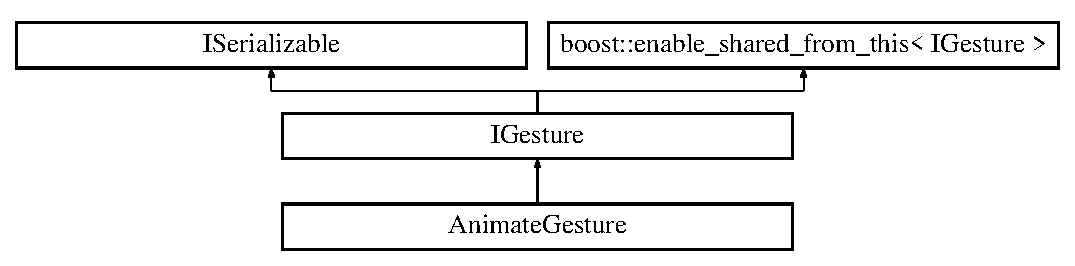
\includegraphics[height=3.000000cm]{class_animate_gesture}
\end{center}
\end{figure}
\subsection*{Classes}
\begin{DoxyCompactItemize}
\item 
struct \hyperlink{struct_animate_gesture_1_1_animation_entry}{Animation\+Entry}
\end{DoxyCompactItemize}
\subsection*{Public Member Functions}
\begin{DoxyCompactItemize}
\item 
\mbox{\Hypertarget{class_animate_gesture_ad111db7e57cc39136a8f073a4ae04d56}\label{class_animate_gesture_ad111db7e57cc39136a8f073a4ae04d56}} 
{\bfseries R\+T\+T\+I\+\_\+\+D\+E\+CL} ()
\item 
\mbox{\Hypertarget{class_animate_gesture_a4db752a229224a48445d80c9168cf758}\label{class_animate_gesture_a4db752a229224a48445d80c9168cf758}} 
\hyperlink{class_animate_gesture_a4db752a229224a48445d80c9168cf758}{Animate\+Gesture} ()
\begin{DoxyCompactList}\small\item\em Construction. \end{DoxyCompactList}\item 
\mbox{\Hypertarget{class_animate_gesture_ac3f44e46cea494d3bbdb0ed72bc0dc48}\label{class_animate_gesture_ac3f44e46cea494d3bbdb0ed72bc0dc48}} 
virtual void \hyperlink{class_animate_gesture_ac3f44e46cea494d3bbdb0ed72bc0dc48}{Serialize} (Json\+::\+Value \&json)
\begin{DoxyCompactList}\small\item\em I\+Serializable interface. \end{DoxyCompactList}\item 
\mbox{\Hypertarget{class_animate_gesture_a2612e96d9fe1002e113fc86005ba1dcc}\label{class_animate_gesture_a2612e96d9fe1002e113fc86005ba1dcc}} 
virtual void {\bfseries Deserialize} (const Json\+::\+Value \&json)
\item 
\mbox{\Hypertarget{class_animate_gesture_afa38a88906eb256fcaabe18e4c18b3eb}\label{class_animate_gesture_afa38a88906eb256fcaabe18e4c18b3eb}} 
virtual bool \hyperlink{class_animate_gesture_afa38a88906eb256fcaabe18e4c18b3eb}{Execute} (Gesture\+Delegate a\+\_\+\+Callback, const \hyperlink{class_params_map}{Params\+Map} \&a\+\_\+\+Params)
\begin{DoxyCompactList}\small\item\em \hyperlink{class_i_gesture}{I\+Gesture} interface. \end{DoxyCompactList}\item 
\mbox{\Hypertarget{class_animate_gesture_a7da2db6241a173a7a0acfc3370b1ada4}\label{class_animate_gesture_a7da2db6241a173a7a0acfc3370b1ada4}} 
virtual bool \hyperlink{class_animate_gesture_a7da2db6241a173a7a0acfc3370b1ada4}{Abort} ()
\begin{DoxyCompactList}\small\item\em Abort this gesture, if true is returned then abort succeeded and callback will N\+OT be invoked. \end{DoxyCompactList}\end{DoxyCompactItemize}
\subsection*{Protected Attributes}
\begin{DoxyCompactItemize}
\item 
\mbox{\Hypertarget{class_animate_gesture_a18ad52314eb12b9f3b1504ca0862517a}\label{class_animate_gesture_a18ad52314eb12b9f3b1504ca0862517a}} 
std\+::vector$<$ \hyperlink{struct_animate_gesture_1_1_animation_entry}{Animation\+Entry} $>$ {\bfseries m\+\_\+\+Animations}
\end{DoxyCompactItemize}
\subsection*{Additional Inherited Members}


\subsection{Detailed Description}
This gesture animates a robot using a built in animation ID. 

The documentation for this class was generated from the following files\+:\begin{DoxyCompactItemize}
\item 
src/gestures/Animate\+Gesture.\+h\item 
src/gestures/Animate\+Gesture.\+cpp\end{DoxyCompactItemize}

\hypertarget{struct_animate_gesture_1_1_animation_entry}{}\section{Animate\+Gesture\+:\+:Animation\+Entry Struct Reference}
\label{struct_animate_gesture_1_1_animation_entry}\index{Animate\+Gesture\+::\+Animation\+Entry@{Animate\+Gesture\+::\+Animation\+Entry}}
\subsection*{Public Member Functions}
\begin{DoxyCompactItemize}
\item 
\mbox{\Hypertarget{struct_animate_gesture_1_1_animation_entry_a0315c5c9ed0bdd3da84c7afd6bd598c1}\label{struct_animate_gesture_1_1_animation_entry_a0315c5c9ed0bdd3da84c7afd6bd598c1}} 
{\bfseries Animation\+Entry} (const std\+::string \&a\+\_\+\+Anim\+Id, const std\+::string \&a\+\_\+\+Required\+Posture)
\end{DoxyCompactItemize}
\subsection*{Public Attributes}
\begin{DoxyCompactItemize}
\item 
\mbox{\Hypertarget{struct_animate_gesture_1_1_animation_entry_a432fcd2ba2ae1e09649f6b911e0d9672}\label{struct_animate_gesture_1_1_animation_entry_a432fcd2ba2ae1e09649f6b911e0d9672}} 
std\+::string {\bfseries m\+\_\+\+Anim\+Id}
\item 
\mbox{\Hypertarget{struct_animate_gesture_1_1_animation_entry_a0aa2dfc297cb7dff927f395c01351a51}\label{struct_animate_gesture_1_1_animation_entry_a0aa2dfc297cb7dff927f395c01351a51}} 
std\+::string {\bfseries m\+\_\+\+Required\+Posture}
\end{DoxyCompactItemize}


The documentation for this struct was generated from the following file\+:\begin{DoxyCompactItemize}
\item 
src/gestures/Animate\+Gesture.\+h\end{DoxyCompactItemize}

\hypertarget{class_asimov_agent}{}\section{Asimov\+Agent Class Reference}
\label{class_asimov_agent}\index{Asimov\+Agent@{Asimov\+Agent}}
Inheritance diagram for Asimov\+Agent\+:\begin{figure}[H]
\begin{center}
\leavevmode
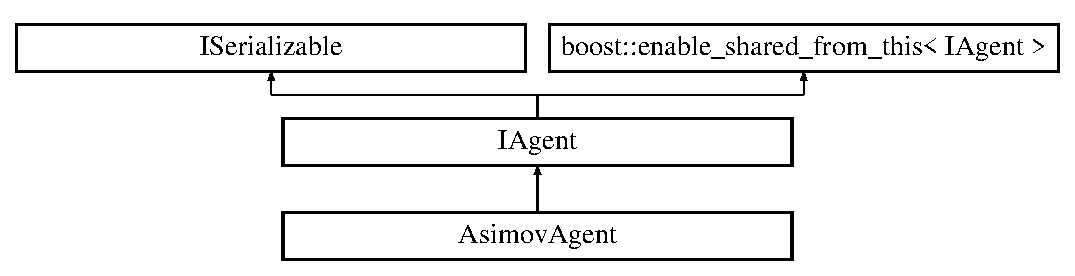
\includegraphics[height=3.000000cm]{class_asimov_agent}
\end{center}
\end{figure}
\subsection*{Public Member Functions}
\begin{DoxyCompactItemize}
\item 
\mbox{\Hypertarget{class_asimov_agent_a423266b1f0892bc41a7acd106a7c757e}\label{class_asimov_agent_a423266b1f0892bc41a7acd106a7c757e}} 
{\bfseries R\+T\+T\+I\+\_\+\+D\+E\+CL} ()
\item 
\mbox{\Hypertarget{class_asimov_agent_a523ddb43c7be34525b42ca61c5c02085}\label{class_asimov_agent_a523ddb43c7be34525b42ca61c5c02085}} 
void \hyperlink{class_asimov_agent_a523ddb43c7be34525b42ca61c5c02085}{Serialize} (Json\+::\+Value \&json)
\begin{DoxyCompactList}\small\item\em I\+Serializable interface. \end{DoxyCompactList}\item 
\mbox{\Hypertarget{class_asimov_agent_add1619cbc6d2af8c46bd2b2bdc6dff24}\label{class_asimov_agent_add1619cbc6d2af8c46bd2b2bdc6dff24}} 
void {\bfseries Deserialize} (const Json\+::\+Value \&json)
\item 
\mbox{\Hypertarget{class_asimov_agent_a1603d40f0b82dabd59821c82345b8868}\label{class_asimov_agent_a1603d40f0b82dabd59821c82345b8868}} 
virtual bool \hyperlink{class_asimov_agent_a1603d40f0b82dabd59821c82345b8868}{On\+Start} ()
\begin{DoxyCompactList}\small\item\em \hyperlink{class_i_agent}{I\+Agent} interface. \end{DoxyCompactList}\item 
\mbox{\Hypertarget{class_asimov_agent_a83a0eb629e37f30960da7623bf9acb58}\label{class_asimov_agent_a83a0eb629e37f30960da7623bf9acb58}} 
virtual bool {\bfseries On\+Stop} ()
\end{DoxyCompactItemize}
\subsection*{Additional Inherited Members}


The documentation for this class was generated from the following files\+:\begin{DoxyCompactItemize}
\item 
src/agent/Asimov\+Agent.\+h\item 
src/agent/Asimov\+Agent.\+cpp\end{DoxyCompactItemize}

\hypertarget{class_attention}{}\section{Attention Class Reference}
\label{class_attention}\index{Attention@{Attention}}


This object is placed on the blackboard when we need self to say anything.  




{\ttfamily \#include $<$Attention.\+h$>$}

Inheritance diagram for Attention\+:\begin{figure}[H]
\begin{center}
\leavevmode
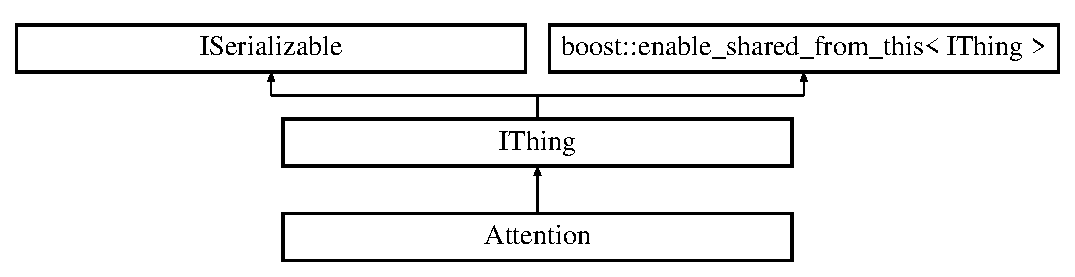
\includegraphics[height=3.000000cm]{class_attention}
\end{center}
\end{figure}
\subsection*{Public Types}
\begin{DoxyCompactItemize}
\item 
\mbox{\Hypertarget{class_attention_ac152b0a7c507c13e8996fc7f2d5e9c31}\label{class_attention_ac152b0a7c507c13e8996fc7f2d5e9c31}} 
typedef boost\+::shared\+\_\+ptr$<$ \hyperlink{class_attention}{Attention} $>$ \hyperlink{class_attention_ac152b0a7c507c13e8996fc7f2d5e9c31}{SP}
\begin{DoxyCompactList}\small\item\em Types. \end{DoxyCompactList}\item 
\mbox{\Hypertarget{class_attention_a3f620dc06985c6e3f447ea904da097a5}\label{class_attention_a3f620dc06985c6e3f447ea904da097a5}} 
typedef boost\+::weak\+\_\+ptr$<$ \hyperlink{class_attention}{Attention} $>$ {\bfseries WP}
\end{DoxyCompactItemize}
\subsection*{Public Member Functions}
\begin{DoxyCompactItemize}
\item 
\mbox{\Hypertarget{class_attention_a01d452288b56763edcfbeab616d0d4bb}\label{class_attention_a01d452288b56763edcfbeab616d0d4bb}} 
{\bfseries R\+T\+T\+I\+\_\+\+D\+E\+CL} ()
\item 
\mbox{\Hypertarget{class_attention_a441783dea3735b46e3c3b2f59f3aa49f}\label{class_attention_a441783dea3735b46e3c3b2f59f3aa49f}} 
virtual void \hyperlink{class_attention_a441783dea3735b46e3c3b2f59f3aa49f}{Serialize} (Json\+::\+Value \&json)
\begin{DoxyCompactList}\small\item\em I\+Serializable interface. \end{DoxyCompactList}\item 
\mbox{\Hypertarget{class_attention_a61c66464d5611b07d758b4cc6b44edf1}\label{class_attention_a61c66464d5611b07d758b4cc6b44edf1}} 
virtual void {\bfseries Deserialize} (const Json\+::\+Value \&json)
\item 
\mbox{\Hypertarget{class_attention_a2774a77497bb424a4e1e6819f5716ce9}\label{class_attention_a2774a77497bb424a4e1e6819f5716ce9}} 
\hyperlink{class_attention_a2774a77497bb424a4e1e6819f5716ce9}{Attention} ()
\begin{DoxyCompactList}\small\item\em Construction. \end{DoxyCompactList}\item 
\mbox{\Hypertarget{class_attention_a4997f530ad9e16dce515de5936a4ea33}\label{class_attention_a4997f530ad9e16dce515de5936a4ea33}} 
{\bfseries Attention} (double a\+\_\+\+Min\+Intent\+Confidence, double a\+\_\+\+Min\+Miss\+Node\+Confidence)
\item 
\mbox{\Hypertarget{class_attention_a281e498ba8e0c9f40964833d357be02d}\label{class_attention_a281e498ba8e0c9f40964833d357be02d}} 
double \hyperlink{class_attention_a281e498ba8e0c9f40964833d357be02d}{Get\+Min\+Intent\+Confidence} () const
\begin{DoxyCompactList}\small\item\em Accessors. \end{DoxyCompactList}\item 
\mbox{\Hypertarget{class_attention_aac64fc991f1fdf46900c39f2f0788f7e}\label{class_attention_aac64fc991f1fdf46900c39f2f0788f7e}} 
void {\bfseries Set\+Min\+Intent\+Confidence} (double a\+\_\+\+Min\+Intent\+Confidence)
\item 
\mbox{\Hypertarget{class_attention_a34a86bb78a2b6dc1ee33fa2d0d290d8b}\label{class_attention_a34a86bb78a2b6dc1ee33fa2d0d290d8b}} 
double {\bfseries Get\+Min\+Miss\+Node\+Confidence} () const
\item 
\mbox{\Hypertarget{class_attention_ad6ebd549f9698013376e208b416890eb}\label{class_attention_ad6ebd549f9698013376e208b416890eb}} 
void {\bfseries Set\+Min\+Miss\+Node\+Confidence} (double a\+\_\+\+Min\+Miss\+Node\+Confidence)
\end{DoxyCompactItemize}
\subsection*{Additional Inherited Members}


\subsection{Detailed Description}
This object is placed on the blackboard when we need self to say anything. 

The documentation for this class was generated from the following files\+:\begin{DoxyCompactItemize}
\item 
src/blackboard/Attention.\+h\item 
src/blackboard/Attention.\+cpp\end{DoxyCompactItemize}

\hypertarget{class_attention_agent}{}\section{Attention\+Agent Class Reference}
\label{class_attention_agent}\index{Attention\+Agent@{Attention\+Agent}}
Inheritance diagram for Attention\+Agent\+:\begin{figure}[H]
\begin{center}
\leavevmode
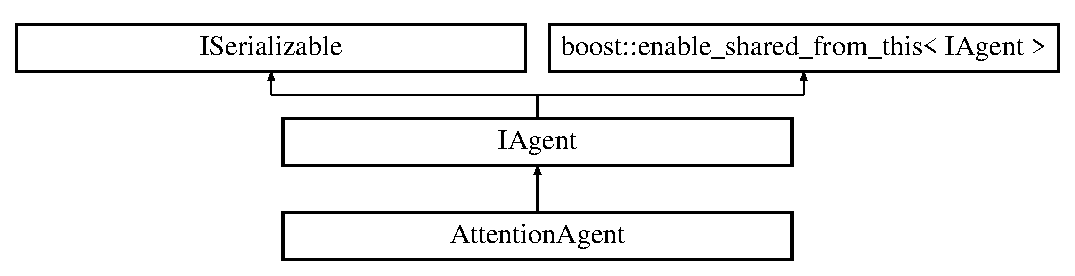
\includegraphics[height=3.000000cm]{class_attention_agent}
\end{center}
\end{figure}
\subsection*{Public Member Functions}
\begin{DoxyCompactItemize}
\item 
\mbox{\Hypertarget{class_attention_agent_a53613e58f92989c8be597d8114a9a40d}\label{class_attention_agent_a53613e58f92989c8be597d8114a9a40d}} 
{\bfseries R\+T\+T\+I\+\_\+\+D\+E\+CL} ()
\item 
\mbox{\Hypertarget{class_attention_agent_a0f4d181576bab8f1a020564289dafbc4}\label{class_attention_agent_a0f4d181576bab8f1a020564289dafbc4}} 
virtual void \hyperlink{class_attention_agent_a0f4d181576bab8f1a020564289dafbc4}{Serialize} (Json\+::\+Value \&json)
\begin{DoxyCompactList}\small\item\em I\+Serializable interface. \end{DoxyCompactList}\item 
\mbox{\Hypertarget{class_attention_agent_a807fd7cf7f37552b1a2c6a0131956973}\label{class_attention_agent_a807fd7cf7f37552b1a2c6a0131956973}} 
virtual void {\bfseries Deserialize} (const Json\+::\+Value \&json)
\item 
\mbox{\Hypertarget{class_attention_agent_a8be527fcfd664f4e68cf6984440ac83c}\label{class_attention_agent_a8be527fcfd664f4e68cf6984440ac83c}} 
virtual bool \hyperlink{class_attention_agent_a8be527fcfd664f4e68cf6984440ac83c}{On\+Start} ()
\begin{DoxyCompactList}\small\item\em \hyperlink{class_i_agent}{I\+Agent} interface. \end{DoxyCompactList}\item 
\mbox{\Hypertarget{class_attention_agent_a55c592103072577ccf44b644288b171c}\label{class_attention_agent_a55c592103072577ccf44b644288b171c}} 
virtual bool {\bfseries On\+Stop} ()
\end{DoxyCompactItemize}
\subsection*{Additional Inherited Members}


The documentation for this class was generated from the following files\+:\begin{DoxyCompactItemize}
\item 
src/agent/Attention\+Agent.\+h\item 
src/agent/Attention\+Agent.\+cpp\end{DoxyCompactItemize}

\hypertarget{class_audio_data}{}\section{Audio\+Data Class Reference}
\label{class_audio_data}\index{Audio\+Data@{Audio\+Data}}


This data type contains raw wave audio data..  




{\ttfamily \#include $<$Audio\+Data.\+h$>$}

Inheritance diagram for Audio\+Data\+:\begin{figure}[H]
\begin{center}
\leavevmode
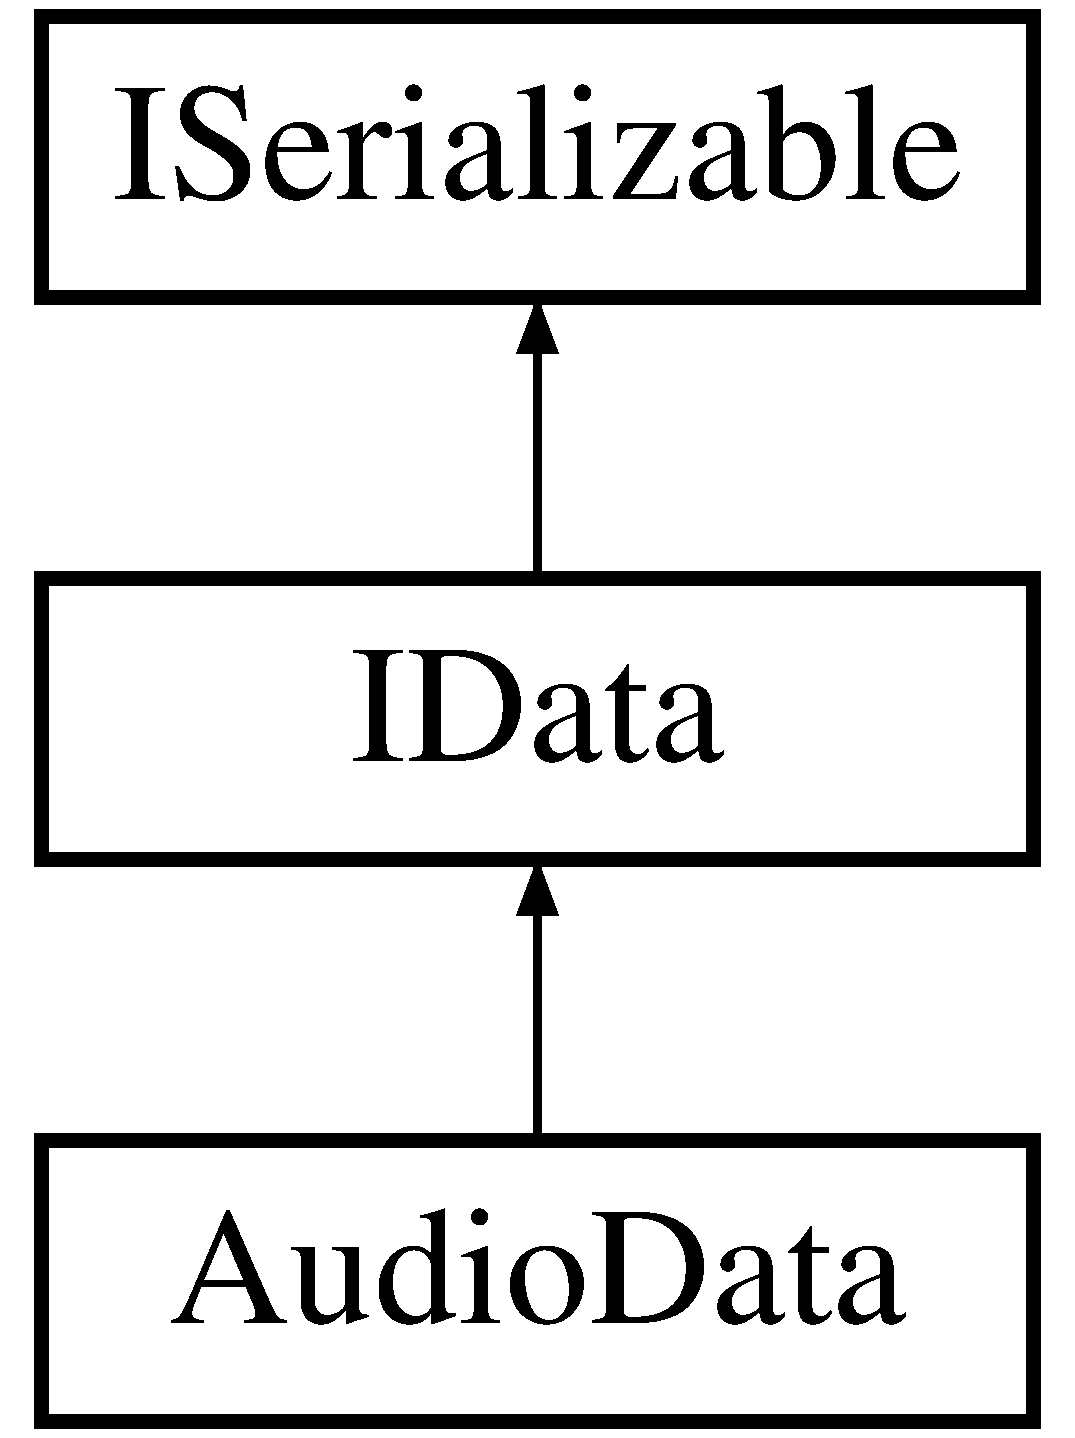
\includegraphics[height=3.000000cm]{class_audio_data}
\end{center}
\end{figure}
\subsection*{Public Member Functions}
\begin{DoxyCompactItemize}
\item 
\mbox{\Hypertarget{class_audio_data_a5575718044a8ddea5b42997c8bcd5d68}\label{class_audio_data_a5575718044a8ddea5b42997c8bcd5d68}} 
{\bfseries R\+T\+T\+I\+\_\+\+D\+E\+CL} ()
\item 
\mbox{\Hypertarget{class_audio_data_a8bb6ddb671a324453713570496f54e59}\label{class_audio_data_a8bb6ddb671a324453713570496f54e59}} 
\hyperlink{class_audio_data_a8bb6ddb671a324453713570496f54e59}{Audio\+Data} ()
\begin{DoxyCompactList}\small\item\em Construction. \end{DoxyCompactList}\item 
\mbox{\Hypertarget{class_audio_data_a916c76fcefbffd41a05cddd529df680e}\label{class_audio_data_a916c76fcefbffd41a05cddd529df680e}} 
{\bfseries Audio\+Data} (const std\+::string \&a\+\_\+\+Wave\+Data, unsigned int a\+\_\+\+Freq, unsigned int a\+\_\+\+Channels, unsigned int a\+\_\+\+B\+PS)
\item 
\mbox{\Hypertarget{class_audio_data_ad1e3dd274ef311cb7c92d68f98ff425d}\label{class_audio_data_ad1e3dd274ef311cb7c92d68f98ff425d}} 
virtual void \hyperlink{class_audio_data_ad1e3dd274ef311cb7c92d68f98ff425d}{Serialize} (Json\+::\+Value \&json)
\begin{DoxyCompactList}\small\item\em I\+Serializable interface. \end{DoxyCompactList}\item 
\mbox{\Hypertarget{class_audio_data_a58a64796ab07807316c1b8b1f4ea49dc}\label{class_audio_data_a58a64796ab07807316c1b8b1f4ea49dc}} 
virtual void {\bfseries Deserialize} (const Json\+::\+Value \&json)
\item 
\mbox{\Hypertarget{class_audio_data_a1cc9349b5edf80a5e0b35e6eb5cb3045}\label{class_audio_data_a1cc9349b5edf80a5e0b35e6eb5cb3045}} 
virtual bool \hyperlink{class_audio_data_a1cc9349b5edf80a5e0b35e6eb5cb3045}{To\+Binary} (std\+::string \&a\+\_\+\+Output)
\begin{DoxyCompactList}\small\item\em \hyperlink{class_i_data}{I\+Data} interface. \end{DoxyCompactList}\item 
\mbox{\Hypertarget{class_audio_data_a9f543a8cd2349e177c861de05ddb9fa8}\label{class_audio_data_a9f543a8cd2349e177c861de05ddb9fa8}} 
virtual bool {\bfseries From\+Binary} (const std\+::string \&a\+\_\+\+Type, const std\+::string \&a\+\_\+\+Input)
\item 
\mbox{\Hypertarget{class_audio_data_aa48989be23c171180a31544dc4059f57}\label{class_audio_data_aa48989be23c171180a31544dc4059f57}} 
const std\+::string \& {\bfseries Get\+Wave\+Data} () const
\item 
\mbox{\Hypertarget{class_audio_data_af99b89b200428c821c6dddc9f823b618}\label{class_audio_data_af99b89b200428c821c6dddc9f823b618}} 
unsigned int {\bfseries Get\+Frequency} () const
\item 
\mbox{\Hypertarget{class_audio_data_a04b3b6246c09ee366260c4b6fb456196}\label{class_audio_data_a04b3b6246c09ee366260c4b6fb456196}} 
unsigned int {\bfseries Get\+Channels} () const
\item 
\mbox{\Hypertarget{class_audio_data_a33ec30b595bcdb8ce9eaf2b8fd8fbf20}\label{class_audio_data_a33ec30b595bcdb8ce9eaf2b8fd8fbf20}} 
unsigned int {\bfseries Get\+B\+PS} () const
\end{DoxyCompactItemize}
\subsection*{Static Public Member Functions}
\begin{DoxyCompactItemize}
\item 
\mbox{\Hypertarget{class_audio_data_a128642493aaf25366ebb1ebc49280f3d}\label{class_audio_data_a128642493aaf25366ebb1ebc49280f3d}} 
static bool {\bfseries Parse\+Audio\+Format} (const std\+::string \&a\+\_\+\+Format, unsigned int \&a\+\_\+\+Freq, unsigned int \&a\+\_\+\+B\+PS, unsigned int \&a\+\_\+\+Channels)
\end{DoxyCompactItemize}


\subsection{Detailed Description}
This data type contains raw wave audio data.. 

The documentation for this class was generated from the following file\+:\begin{DoxyCompactItemize}
\item 
src/sensors/Audio\+Data.\+h\end{DoxyCompactItemize}

\hypertarget{class_beat_extractor}{}\section{Beat\+Extractor Class Reference}
\label{class_beat_extractor}\index{Beat\+Extractor@{Beat\+Extractor}}


{\ttfamily \#include $<$Beat\+Extractor.\+h$>$}

Inheritance diagram for Beat\+Extractor\+:\begin{figure}[H]
\begin{center}
\leavevmode
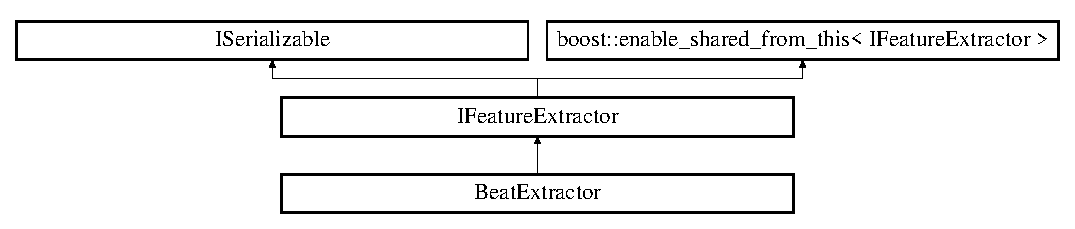
\includegraphics[height=2.625000cm]{class_beat_extractor}
\end{center}
\end{figure}
\subsection*{Public Member Functions}
\begin{DoxyCompactItemize}
\item 
\mbox{\Hypertarget{class_beat_extractor_ac3b3f8d1723f4e4992e918e02265602a}\label{class_beat_extractor_ac3b3f8d1723f4e4992e918e02265602a}} 
{\bfseries R\+T\+T\+I\+\_\+\+D\+E\+CL} ()
\item 
\mbox{\Hypertarget{class_beat_extractor_a3c8410a38f7750f44160ddf21ff21336}\label{class_beat_extractor_a3c8410a38f7750f44160ddf21ff21336}} 
\hyperlink{class_beat_extractor_a3c8410a38f7750f44160ddf21ff21336}{Beat\+Extractor} ()
\begin{DoxyCompactList}\small\item\em Construction. \end{DoxyCompactList}\item 
\mbox{\Hypertarget{class_beat_extractor_a9f8e101a85fc83b9613c1fa1aa4db8b1}\label{class_beat_extractor_a9f8e101a85fc83b9613c1fa1aa4db8b1}} 
virtual void \hyperlink{class_beat_extractor_a9f8e101a85fc83b9613c1fa1aa4db8b1}{Serialize} (Json\+::\+Value \&json)
\begin{DoxyCompactList}\small\item\em I\+Serialziable interface. \end{DoxyCompactList}\item 
\mbox{\Hypertarget{class_beat_extractor_a4375f7f44e267b8e79c87644c22b6d08}\label{class_beat_extractor_a4375f7f44e267b8e79c87644c22b6d08}} 
virtual void {\bfseries Deserialize} (const Json\+::\+Value \&json)
\item 
\mbox{\Hypertarget{class_beat_extractor_ae0fda2270d14b1a8d712dcfda853b64c}\label{class_beat_extractor_ae0fda2270d14b1a8d712dcfda853b64c}} 
virtual const char $\ast$ \hyperlink{class_beat_extractor_ae0fda2270d14b1a8d712dcfda853b64c}{Get\+Name} () const
\begin{DoxyCompactList}\small\item\em \hyperlink{class_i_feature_extractor}{I\+Feature\+Extractor} interface. \end{DoxyCompactList}\item 
\mbox{\Hypertarget{class_beat_extractor_ae6823071ceed497f3e5f33a799c1adc5}\label{class_beat_extractor_ae6823071ceed497f3e5f33a799c1adc5}} 
virtual bool {\bfseries On\+Start} ()
\item 
\mbox{\Hypertarget{class_beat_extractor_a4e6b9f8229e11f66110bf1ec05f3506b}\label{class_beat_extractor_a4e6b9f8229e11f66110bf1ec05f3506b}} 
virtual bool {\bfseries On\+Stop} ()
\end{DoxyCompactItemize}
\subsection*{Additional Inherited Members}


\subsection{Detailed Description}
This filter doesn\textquotesingle{}t filter audio, it just detects music beats and posts a Beat object to the blackboard when a music beat is detected. 

The documentation for this class was generated from the following files\+:\begin{DoxyCompactItemize}
\item 
src/extractors/Beat\+Extractor.\+h\item 
src/extractors/Beat\+Extractor.\+cpp\end{DoxyCompactItemize}

\hypertarget{class_black_board}{}\section{Black\+Board Class Reference}
\label{class_black_board}\index{Black\+Board@{Black\+Board}}


The \hyperlink{class_black_board}{Black\+Board} class acts as the central publish/subscribe system for all agents, classifiers, and extractors.  




{\ttfamily \#include $<$Black\+Board.\+h$>$}

Inheritance diagram for Black\+Board\+:\begin{figure}[H]
\begin{center}
\leavevmode
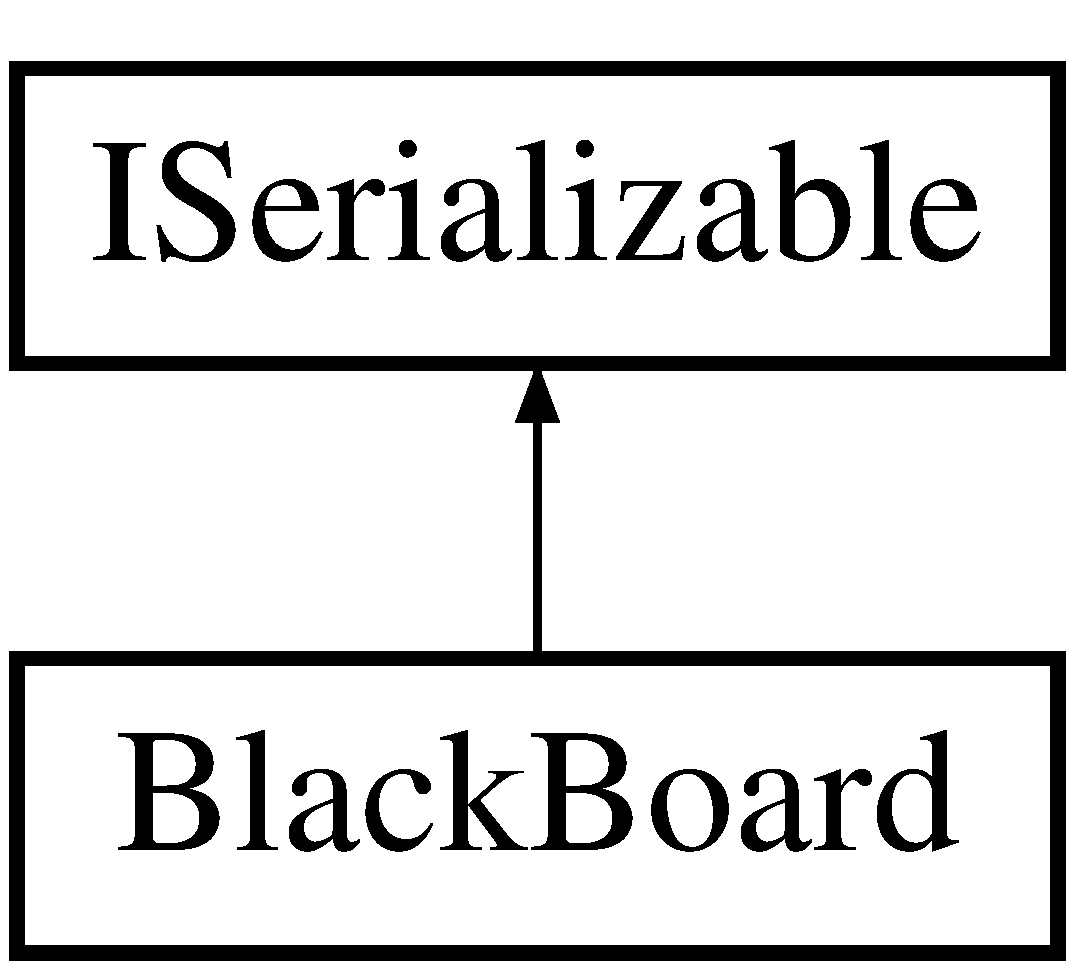
\includegraphics[height=2.000000cm]{class_black_board}
\end{center}
\end{figure}
\subsection*{Public Types}
\begin{DoxyCompactItemize}
\item 
\mbox{\Hypertarget{class_black_board_a34c71e0cce3bbfd34bd9fd91607b01c0}\label{class_black_board_a34c71e0cce3bbfd34bd9fd91607b01c0}} 
typedef I\+Thing\+::\+Thing\+List \hyperlink{class_black_board_a34c71e0cce3bbfd34bd9fd91607b01c0}{Thing\+List}
\begin{DoxyCompactList}\small\item\em Types. \end{DoxyCompactList}\end{DoxyCompactItemize}
\subsection*{Public Member Functions}
\begin{DoxyCompactItemize}
\item 
\mbox{\Hypertarget{class_black_board_adab334b501f4d17adf3b20395a65ca8a}\label{class_black_board_adab334b501f4d17adf3b20395a65ca8a}} 
{\bfseries R\+T\+T\+I\+\_\+\+D\+E\+CL} ()
\item 
\mbox{\Hypertarget{class_black_board_a34e2a107547d7217a7705d6c88058db3}\label{class_black_board_a34e2a107547d7217a7705d6c88058db3}} 
\hyperlink{class_black_board_a34e2a107547d7217a7705d6c88058db3}{Black\+Board} ()
\begin{DoxyCompactList}\small\item\em Construction. \end{DoxyCompactList}\item 
\mbox{\Hypertarget{class_black_board_a7c0ededc79c06f51a4042392add4e964}\label{class_black_board_a7c0ededc79c06f51a4042392add4e964}} 
virtual void \hyperlink{class_black_board_a7c0ededc79c06f51a4042392add4e964}{Serialize} (Json\+::\+Value \&json)
\begin{DoxyCompactList}\small\item\em I\+Serializable interface. \end{DoxyCompactList}\item 
\mbox{\Hypertarget{class_black_board_a263a37bd1fdbb46db6def0cd0503d0c5}\label{class_black_board_a263a37bd1fdbb46db6def0cd0503d0c5}} 
virtual void {\bfseries Deserialize} (const Json\+::\+Value \&json)
\item 
\mbox{\Hypertarget{class_black_board_a13d70fb27ef59b83635fed85ced2d3eb}\label{class_black_board_a13d70fb27ef59b83635fed85ced2d3eb}} 
const \hyperlink{class_i_thing_a6e95654aef6362c48b9a2fd44a1f970a}{I\+Thing\+::\+SP} \& \hyperlink{class_black_board_a13d70fb27ef59b83635fed85ced2d3eb}{Get\+Perception\+Root} () const
\begin{DoxyCompactList}\small\item\em Accessors. \end{DoxyCompactList}\item 
\mbox{\Hypertarget{class_black_board_aa2baa55ec0fa21acc396add9e1ec4d1d}\label{class_black_board_aa2baa55ec0fa21acc396add9e1ec4d1d}} 
const \hyperlink{class_i_thing_a6e95654aef6362c48b9a2fd44a1f970a}{I\+Thing\+::\+SP} \& {\bfseries Get\+Agency\+Root} () const
\item 
\mbox{\Hypertarget{class_black_board_a17c8cf8fee4533eb0ac37a7a33e1d3aa}\label{class_black_board_a17c8cf8fee4533eb0ac37a7a33e1d3aa}} 
const \hyperlink{class_i_thing_a6e95654aef6362c48b9a2fd44a1f970a}{I\+Thing\+::\+SP} \& {\bfseries Get\+Models\+Root} () const
\item 
\mbox{\Hypertarget{class_black_board_aa54d6d7a39e067e0091e0358951b598b}\label{class_black_board_aa54d6d7a39e067e0091e0358951b598b}} 
\hyperlink{class_i_thing_a6e95654aef6362c48b9a2fd44a1f970a}{I\+Thing\+::\+SP} {\bfseries Find\+Thing} (const std\+::string \&a\+\_\+\+G\+U\+ID) const
\item 
\mbox{\Hypertarget{class_black_board_adb449e10fc27b8f50dc3b00c63a188c2}\label{class_black_board_adb449e10fc27b8f50dc3b00c63a188c2}} 
bool \hyperlink{class_black_board_adb449e10fc27b8f50dc3b00c63a188c2}{Start} ()
\begin{DoxyCompactList}\small\item\em Initialize this blackboard. \end{DoxyCompactList}\item 
\mbox{\Hypertarget{class_black_board_ab1f9089fcea4cb6739401df5d72301cc}\label{class_black_board_ab1f9089fcea4cb6739401df5d72301cc}} 
bool {\bfseries Stop} ()
\item 
void \hyperlink{class_black_board_ae5c15e743e9abd413c1711a3091b6da8}{Add\+Thing} (const \hyperlink{class_i_thing_a6e95654aef6362c48b9a2fd44a1f970a}{I\+Thing\+::\+SP} \&a\+\_\+sp\+Thing)
\item 
\mbox{\Hypertarget{class_black_board_a64c506b6e6a6eaaeac52c03ecfe6b4a5}\label{class_black_board_a64c506b6e6a6eaaeac52c03ecfe6b4a5}} 
bool \hyperlink{class_black_board_a64c506b6e6a6eaaeac52c03ecfe6b4a5}{Remove\+Thing} (\hyperlink{class_i_thing}{I\+Thing} $\ast$a\+\_\+p\+Thing)
\begin{DoxyCompactList}\small\item\em This removes the specific thing from the board. \end{DoxyCompactList}\item 
void \hyperlink{class_black_board_a6e3a81af31e182047d78adf2131f8d09}{Subscribe\+To\+Type} (const std\+::string \&a\+\_\+\+Type, Delegate$<$ const \hyperlink{class_thing_event}{Thing\+Event} \&$>$ a\+\_\+callback, Thing\+Event\+Type event\+Mask=T\+E\+\_\+\+A\+LL)
\item 
bool \hyperlink{class_black_board_a743f02f77a5d7008b510459dbcac69d6}{Unsubscribe\+From\+Type} (const std\+::string \&a\+\_\+\+Type, void $\ast$a\+\_\+p\+Object=N\+U\+LL)
\item 
void \hyperlink{class_black_board_a64acc3b0a151c7124341ec4b67b2a23c}{On\+Thing\+Event} (const \hyperlink{class_thing_event}{Thing\+Event} \&thing)
\item 
\mbox{\Hypertarget{class_black_board_a497c4e96a9fe9b38c003c69804af039f}\label{class_black_board_a497c4e96a9fe9b38c003c69804af039f}} 
void {\bfseries Register\+Thing} (const \hyperlink{class_i_thing_a6e95654aef6362c48b9a2fd44a1f970a}{I\+Thing\+::\+SP} \&a\+\_\+sp\+Thing)
\item 
\mbox{\Hypertarget{class_black_board_a031276d932dff376433465ce51930d0a}\label{class_black_board_a031276d932dff376433465ce51930d0a}} 
void {\bfseries Unregister\+Thing} (const \hyperlink{class_i_thing_a6e95654aef6362c48b9a2fd44a1f970a}{I\+Thing\+::\+SP} \&a\+\_\+sp\+Thing)
\item 
\mbox{\Hypertarget{class_black_board_aa4d9fbeac301adf593f08db2b6e24b74}\label{class_black_board_aa4d9fbeac301adf593f08db2b6e24b74}} 
void \hyperlink{class_black_board_aa4d9fbeac301adf593f08db2b6e24b74}{Subscribe\+To\+Type} (const R\+T\+TI \&type, Delegate$<$ const \hyperlink{class_thing_event}{Thing\+Event} \&$>$ a\+\_\+callback, Thing\+Event\+Type event\+Mask=T\+E\+\_\+\+A\+LL)
\begin{DoxyCompactList}\small\item\em Deprecated Interface. \end{DoxyCompactList}\item 
\mbox{\Hypertarget{class_black_board_a44f2cc7495a0a89e50813f5420ced0e5}\label{class_black_board_a44f2cc7495a0a89e50813f5420ced0e5}} 
bool {\bfseries Unsubscribe\+From\+Type} (const R\+T\+TI \&type, void $\ast$a\+\_\+p\+Object=N\+U\+LL)
\end{DoxyCompactItemize}


\subsection{Detailed Description}
The \hyperlink{class_black_board}{Black\+Board} class acts as the central publish/subscribe system for all agents, classifiers, and extractors. 

\subsection{Member Function Documentation}
\mbox{\Hypertarget{class_black_board_ae5c15e743e9abd413c1711a3091b6da8}\label{class_black_board_ae5c15e743e9abd413c1711a3091b6da8}} 
\index{Black\+Board@{Black\+Board}!Add\+Thing@{Add\+Thing}}
\index{Add\+Thing@{Add\+Thing}!Black\+Board@{Black\+Board}}
\subsubsection{\texorpdfstring{Add\+Thing()}{AddThing()}}
{\footnotesize\ttfamily void Black\+Board\+::\+Add\+Thing (\begin{DoxyParamCaption}\item[{const \hyperlink{class_i_thing_a6e95654aef6362c48b9a2fd44a1f970a}{I\+Thing\+::\+SP} \&}]{a\+\_\+sp\+Thing }\end{DoxyParamCaption})}

Add a concept to this \hyperlink{class_black_board}{Black\+Board}, this concept will automatically be connected to other concepts to produce a \hyperlink{class_goal}{Goal} in the end. This object takes ownership of the provided object and will delete the concept once a goal is produced. \mbox{\Hypertarget{class_black_board_a64acc3b0a151c7124341ec4b67b2a23c}\label{class_black_board_a64acc3b0a151c7124341ec4b67b2a23c}} 
\index{Black\+Board@{Black\+Board}!On\+Thing\+Event@{On\+Thing\+Event}}
\index{On\+Thing\+Event@{On\+Thing\+Event}!Black\+Board@{Black\+Board}}
\subsubsection{\texorpdfstring{On\+Thing\+Event()}{OnThingEvent()}}
{\footnotesize\ttfamily void Black\+Board\+::\+On\+Thing\+Event (\begin{DoxyParamCaption}\item[{const \hyperlink{class_thing_event}{Thing\+Event} \&}]{thing }\end{DoxyParamCaption})}

Invoke this function to pass a event to all subscribers for a given object type. This is invoked automatically by \hyperlink{class_black_board_ae5c15e743e9abd413c1711a3091b6da8}{Add\+Thing()}, \hyperlink{class_black_board_a64c506b6e6a6eaaeac52c03ecfe6b4a5}{Remove\+Thing()}, and when a state is changed on a \hyperlink{class_i_thing}{I\+Thing} object. \mbox{\Hypertarget{class_black_board_a6e3a81af31e182047d78adf2131f8d09}\label{class_black_board_a6e3a81af31e182047d78adf2131f8d09}} 
\index{Black\+Board@{Black\+Board}!Subscribe\+To\+Type@{Subscribe\+To\+Type}}
\index{Subscribe\+To\+Type@{Subscribe\+To\+Type}!Black\+Board@{Black\+Board}}
\subsubsection{\texorpdfstring{Subscribe\+To\+Type()}{SubscribeToType()}}
{\footnotesize\ttfamily void Black\+Board\+::\+Subscribe\+To\+Type (\begin{DoxyParamCaption}\item[{const std\+::string \&}]{a\+\_\+\+Type,  }\item[{Delegate$<$ const \hyperlink{class_thing_event}{Thing\+Event} \&$>$}]{a\+\_\+callback,  }\item[{Thing\+Event\+Type}]{event\+Mask = {\ttfamily TE\+\_\+ALL} }\end{DoxyParamCaption})}

Subscribe to any objects of the given type getting added to this Blackboard. Optionally, the user may subscribe to only certain events. \mbox{\Hypertarget{class_black_board_a743f02f77a5d7008b510459dbcac69d6}\label{class_black_board_a743f02f77a5d7008b510459dbcac69d6}} 
\index{Black\+Board@{Black\+Board}!Unsubscribe\+From\+Type@{Unsubscribe\+From\+Type}}
\index{Unsubscribe\+From\+Type@{Unsubscribe\+From\+Type}!Black\+Board@{Black\+Board}}
\subsubsection{\texorpdfstring{Unsubscribe\+From\+Type()}{UnsubscribeFromType()}}
{\footnotesize\ttfamily bool Black\+Board\+::\+Unsubscribe\+From\+Type (\begin{DoxyParamCaption}\item[{const std\+::string \&}]{a\+\_\+\+Type,  }\item[{void $\ast$}]{a\+\_\+p\+Object = {\ttfamily NULL} }\end{DoxyParamCaption})}

Unsubscribe the given type and callback object. If a\+\_\+p\+Object is N\+U\+LL, then all callbacks for the given type are cleared. Returns false if no match was found. 

The documentation for this class was generated from the following files\+:\begin{DoxyCompactItemize}
\item 
src/blackboard/Black\+Board.\+h\item 
src/blackboard/Black\+Board.\+cpp\end{DoxyCompactItemize}

\hypertarget{class_calculate}{}\section{Calculate Class Reference}
\label{class_calculate}\index{Calculate@{Calculate}}


This object is placed on the blackboard when we need self to calculate something.  




{\ttfamily \#include $<$Calculate.\+h$>$}

Inheritance diagram for Calculate\+:\begin{figure}[H]
\begin{center}
\leavevmode
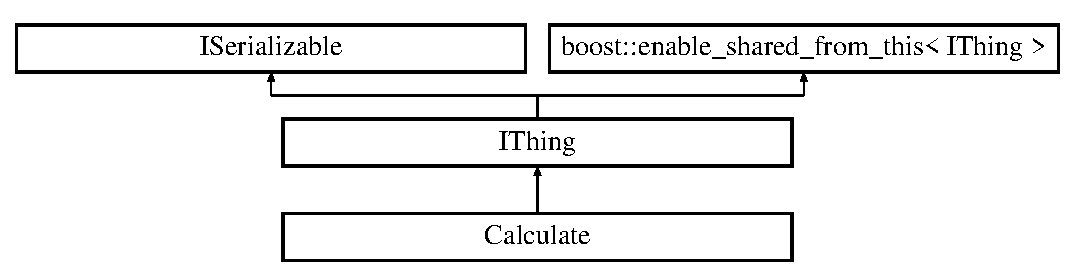
\includegraphics[height=3.000000cm]{class_calculate}
\end{center}
\end{figure}
\subsection*{Public Types}
\begin{DoxyCompactItemize}
\item 
\mbox{\Hypertarget{class_calculate_a45027220b95e94879281ce0d57423082}\label{class_calculate_a45027220b95e94879281ce0d57423082}} 
typedef boost\+::shared\+\_\+ptr$<$ \hyperlink{class_calculate}{Calculate} $>$ \hyperlink{class_calculate_a45027220b95e94879281ce0d57423082}{SP}
\begin{DoxyCompactList}\small\item\em Types. \end{DoxyCompactList}\item 
\mbox{\Hypertarget{class_calculate_a25c76395c135b19bced534cfcf64eb64}\label{class_calculate_a25c76395c135b19bced534cfcf64eb64}} 
typedef boost\+::weak\+\_\+ptr$<$ \hyperlink{class_calculate}{Calculate} $>$ {\bfseries WP}
\end{DoxyCompactItemize}
\subsection*{Public Member Functions}
\begin{DoxyCompactItemize}
\item 
\mbox{\Hypertarget{class_calculate_abf54cf9803fcf27231ddb4fc8de521fc}\label{class_calculate_abf54cf9803fcf27231ddb4fc8de521fc}} 
{\bfseries R\+T\+T\+I\+\_\+\+D\+E\+CL} ()
\item 
\mbox{\Hypertarget{class_calculate_a777e77f559b8c54ff730eb37fd2ae6a5}\label{class_calculate_a777e77f559b8c54ff730eb37fd2ae6a5}} 
virtual void \hyperlink{class_calculate_a777e77f559b8c54ff730eb37fd2ae6a5}{Serialize} (Json\+::\+Value \&json)
\begin{DoxyCompactList}\small\item\em I\+Serializable interface. \end{DoxyCompactList}\item 
\mbox{\Hypertarget{class_calculate_a1a8f1974ec5b7b40fbc0dde839d2b1b5}\label{class_calculate_a1a8f1974ec5b7b40fbc0dde839d2b1b5}} 
virtual void {\bfseries Deserialize} (const Json\+::\+Value \&json)
\item 
\mbox{\Hypertarget{class_calculate_a9324cfcffaf7004813243ab39b003c66}\label{class_calculate_a9324cfcffaf7004813243ab39b003c66}} 
\hyperlink{class_calculate_a9324cfcffaf7004813243ab39b003c66}{Calculate} ()
\begin{DoxyCompactList}\small\item\em Construction. \end{DoxyCompactList}\item 
\mbox{\Hypertarget{class_calculate_afb33778c92ef17d52f11471cbea5be75}\label{class_calculate_afb33778c92ef17d52f11471cbea5be75}} 
{\bfseries Calculate} (const std\+::string \&a\+\_\+\+Data, const std\+::string \&a\+\_\+\+Arithmetic, const std\+::string \&a\+\_\+\+Key)
\item 
\mbox{\Hypertarget{class_calculate_a9f653444641c2b365a4c6722017f6293}\label{class_calculate_a9f653444641c2b365a4c6722017f6293}} 
const std\+::string \& \hyperlink{class_calculate_a9f653444641c2b365a4c6722017f6293}{Get\+Data} () const
\begin{DoxyCompactList}\small\item\em Accessors. \end{DoxyCompactList}\item 
\mbox{\Hypertarget{class_calculate_a1e1f0c9814392a129027be0a21cad11f}\label{class_calculate_a1e1f0c9814392a129027be0a21cad11f}} 
const std\+::string \& {\bfseries Get\+Arithmetic} () const
\item 
\mbox{\Hypertarget{class_calculate_a41dadfb963f4b2de5413c25dccc7cced}\label{class_calculate_a41dadfb963f4b2de5413c25dccc7cced}} 
const std\+::string \& {\bfseries Get\+Key} () const
\end{DoxyCompactItemize}
\subsection*{Additional Inherited Members}


\subsection{Detailed Description}
This object is placed on the blackboard when we need self to calculate something. 

The documentation for this class was generated from the following files\+:\begin{DoxyCompactItemize}
\item 
src/blackboard/Calculate.\+h\item 
src/blackboard/Calculate.\+cpp\end{DoxyCompactItemize}

\hypertarget{class_camera}{}\section{Camera Class Reference}
\label{class_camera}\index{Camera@{Camera}}


Base class for a \hyperlink{class_camera}{Camera} sensor class that collects \hyperlink{class_video_data}{Video\+Data}. This is not a actual implementation, see Nao\+Camera.  




{\ttfamily \#include $<$Camera.\+h$>$}

Inheritance diagram for Camera\+:\begin{figure}[H]
\begin{center}
\leavevmode
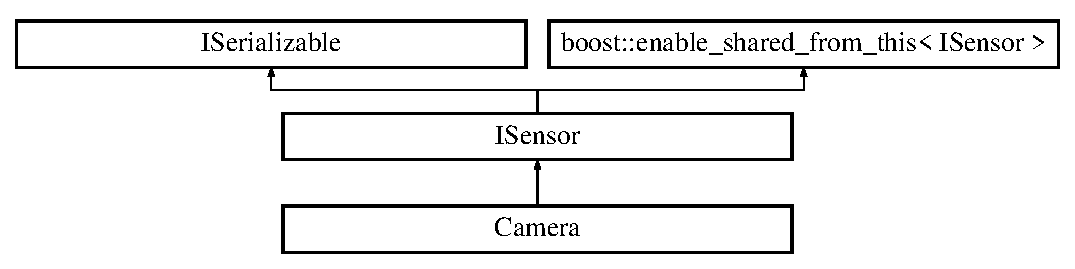
\includegraphics[height=3.000000cm]{class_camera}
\end{center}
\end{figure}
\subsection*{Public Member Functions}
\begin{DoxyCompactItemize}
\item 
\mbox{\Hypertarget{class_camera_abee8bc9a9c1ebee8a809b2fb8e436950}\label{class_camera_abee8bc9a9c1ebee8a809b2fb8e436950}} 
{\bfseries R\+T\+T\+I\+\_\+\+D\+E\+CL} ()
\item 
\mbox{\Hypertarget{class_camera_a5b70be7fddf2ccf074890a7e7b369188}\label{class_camera_a5b70be7fddf2ccf074890a7e7b369188}} 
virtual void \hyperlink{class_camera_a5b70be7fddf2ccf074890a7e7b369188}{Serialize} (Json\+::\+Value \&json)
\begin{DoxyCompactList}\small\item\em I\+Serialiazable interface. \end{DoxyCompactList}\item 
\mbox{\Hypertarget{class_camera_a82ec2a9bb8493f2c4bbdb97cd79dfd94}\label{class_camera_a82ec2a9bb8493f2c4bbdb97cd79dfd94}} 
virtual void {\bfseries Deserialize} (const Json\+::\+Value \&json)
\item 
\mbox{\Hypertarget{class_camera_a982c2ab097483c212e1267485848819d}\label{class_camera_a982c2ab097483c212e1267485848819d}} 
virtual const char $\ast$ \hyperlink{class_camera_a982c2ab097483c212e1267485848819d}{Get\+Sensor\+Name} ()
\begin{DoxyCompactList}\small\item\em \hyperlink{class_i_sensor}{I\+Sensor} interface. \end{DoxyCompactList}\item 
\mbox{\Hypertarget{class_camera_a0601adae3ffbef3152cab59d423fc678}\label{class_camera_a0601adae3ffbef3152cab59d423fc678}} 
virtual const char $\ast$ {\bfseries Get\+Data\+Type} ()
\item 
\mbox{\Hypertarget{class_camera_a10d9f7d28581f448474b65ca9755caa3}\label{class_camera_a10d9f7d28581f448474b65ca9755caa3}} 
virtual const char $\ast$ {\bfseries Get\+Binary\+Type} ()
\item 
\mbox{\Hypertarget{class_camera_a7ca83b9c76148375de7f2c38c7443824}\label{class_camera_a7ca83b9c76148375de7f2c38c7443824}} 
virtual bool \hyperlink{class_camera_a7ca83b9c76148375de7f2c38c7443824}{On\+Start} ()
\begin{DoxyCompactList}\small\item\em This is invoked when the first subscriber subscribes to this sensor. \end{DoxyCompactList}\item 
\mbox{\Hypertarget{class_camera_af42a31534de2673e62f4b000d96ddd4c}\label{class_camera_af42a31534de2673e62f4b000d96ddd4c}} 
virtual bool \hyperlink{class_camera_af42a31534de2673e62f4b000d96ddd4c}{On\+Stop} ()
\begin{DoxyCompactList}\small\item\em This is invoked when the last subscriber un-\/subscribes. \end{DoxyCompactList}\item 
\mbox{\Hypertarget{class_camera_aecd7262c9ddd921cd7d6223ee84586ae}\label{class_camera_aecd7262c9ddd921cd7d6223ee84586ae}} 
virtual void \hyperlink{class_camera_aecd7262c9ddd921cd7d6223ee84586ae}{On\+Pause} ()
\begin{DoxyCompactList}\small\item\em This is invoked to pause this sensor. \end{DoxyCompactList}\item 
\mbox{\Hypertarget{class_camera_afb0a4e93bb0bb354d3fa3e5b5631a247}\label{class_camera_afb0a4e93bb0bb354d3fa3e5b5631a247}} 
virtual void \hyperlink{class_camera_afb0a4e93bb0bb354d3fa3e5b5631a247}{On\+Resume} ()
\begin{DoxyCompactList}\small\item\em This is invoked to restart this sensor. \end{DoxyCompactList}\end{DoxyCompactItemize}
\subsection*{Protected Attributes}
\begin{DoxyCompactItemize}
\item 
\mbox{\Hypertarget{class_camera_aa5bca0acb4af13119c6d5c498dafd59d}\label{class_camera_aa5bca0acb4af13119c6d5c498dafd59d}} 
float \hyperlink{class_camera_aa5bca0acb4af13119c6d5c498dafd59d}{m\+\_\+f\+Frames\+Per\+Sec}
\begin{DoxyCompactList}\small\item\em Data. \end{DoxyCompactList}\end{DoxyCompactItemize}
\subsection*{Additional Inherited Members}


\subsection{Detailed Description}
Base class for a \hyperlink{class_camera}{Camera} sensor class that collects \hyperlink{class_video_data}{Video\+Data}. This is not a actual implementation, see Nao\+Camera. 

The documentation for this class was generated from the following files\+:\begin{DoxyCompactItemize}
\item 
src/sensors/Camera.\+h\item 
src/sensors/Camera.\+cpp\end{DoxyCompactItemize}

\hypertarget{class_classifier_manager}{}\section{Classifier\+Manager Class Reference}
\label{class_classifier_manager}\index{Classifier\+Manager@{Classifier\+Manager}}


{\ttfamily \#include $<$Classifier\+Manager.\+h$>$}

\subsection*{Public Types}
\begin{DoxyCompactItemize}
\item 
\mbox{\Hypertarget{class_classifier_manager_aae20ce0b00515992da2c2375decebdd3}\label{class_classifier_manager_aae20ce0b00515992da2c2375decebdd3}} 
typedef std\+::list$<$ \hyperlink{class_i_classifier_a532d21507aef94011669a0b73bd49c2d}{I\+Classifier\+::\+SP} $>$ \hyperlink{class_classifier_manager_aae20ce0b00515992da2c2375decebdd3}{Classifier\+List}
\begin{DoxyCompactList}\small\item\em Types. \end{DoxyCompactList}\end{DoxyCompactItemize}
\subsection*{Public Member Functions}
\begin{DoxyCompactItemize}
\item 
\mbox{\Hypertarget{class_classifier_manager_a1af886a1f3c7bb0fe6a804978e6ef431}\label{class_classifier_manager_a1af886a1f3c7bb0fe6a804978e6ef431}} 
\hyperlink{class_classifier_manager_a1af886a1f3c7bb0fe6a804978e6ef431}{Classifier\+Manager} ()
\begin{DoxyCompactList}\small\item\em Construction. \end{DoxyCompactList}\item 
\mbox{\Hypertarget{class_classifier_manager_a76f262b018bee815fa1772edd665c61e}\label{class_classifier_manager_a76f262b018bee815fa1772edd665c61e}} 
const \hyperlink{class_classifier_manager_aae20ce0b00515992da2c2375decebdd3}{Classifier\+List} \& \hyperlink{class_classifier_manager_a76f262b018bee815fa1772edd665c61e}{Get\+Classifier\+List} () const
\begin{DoxyCompactList}\small\item\em Accessors. \end{DoxyCompactList}\item 
\mbox{\Hypertarget{class_classifier_manager_a80379c1004db60dbd1c39baa522732b7}\label{class_classifier_manager_a80379c1004db60dbd1c39baa522732b7}} 
bool \hyperlink{class_classifier_manager_a80379c1004db60dbd1c39baa522732b7}{Start} ()
\begin{DoxyCompactList}\small\item\em Start this manager, initializes all available Classifier objects. \end{DoxyCompactList}\item 
\mbox{\Hypertarget{class_classifier_manager_ab4ba7a475ee06b7e58e557da8cf49b13}\label{class_classifier_manager_ab4ba7a475ee06b7e58e557da8cf49b13}} 
bool \hyperlink{class_classifier_manager_ab4ba7a475ee06b7e58e557da8cf49b13}{Stop} ()
\begin{DoxyCompactList}\small\item\em Stop this manager. \end{DoxyCompactList}\item 
\mbox{\Hypertarget{class_classifier_manager_aa9710c99ee57697553c8d6329dfc409f}\label{class_classifier_manager_aa9710c99ee57697553c8d6329dfc409f}} 
{\footnotesize template$<$typename T $>$ }\\T $\ast$ {\bfseries Find\+Classifier} () const
\item 
\mbox{\Hypertarget{class_classifier_manager_ad811cdc506ae96eecc90f055b01bea69}\label{class_classifier_manager_ad811cdc506ae96eecc90f055b01bea69}} 
{\footnotesize template$<$typename T $>$ }\\T $\ast$ {\bfseries Get\+Classifier} ()
\end{DoxyCompactItemize}


\subsection{Detailed Description}
This class manages all active classifier instances. This classifiers subscribe to sensors and add concepts to the \hyperlink{class_black_board}{Black\+Board} object contained by the \hyperlink{class_self_instance}{Self\+Instance}. 

The documentation for this class was generated from the following files\+:\begin{DoxyCompactItemize}
\item 
src/classifiers/Classifier\+Manager.\+h\item 
src/classifiers/Classifier\+Manager.\+cpp\end{DoxyCompactItemize}

\hypertarget{struct_i_text_classifier_proxy_1_1_classify_result}{}\section{I\+Text\+Classifier\+Proxy\+:\+:Classify\+Result Struct Reference}
\label{struct_i_text_classifier_proxy_1_1_classify_result}\index{I\+Text\+Classifier\+Proxy\+::\+Classify\+Result@{I\+Text\+Classifier\+Proxy\+::\+Classify\+Result}}


This struct is passed back through the callback to the \hyperlink{class_text_classifier}{Text\+Classifier} with the results of this proxy.  




{\ttfamily \#include $<$I\+Text\+Classifier\+Proxy.\+h$>$}

\subsection*{Public Attributes}
\begin{DoxyCompactItemize}
\item 
\mbox{\Hypertarget{struct_i_text_classifier_proxy_1_1_classify_result_a55fac4bc1e0fe33b7465ec2ef3050c42}\label{struct_i_text_classifier_proxy_1_1_classify_result_a55fac4bc1e0fe33b7465ec2ef3050c42}} 
double {\bfseries m\+\_\+f\+Confidence}
\item 
\mbox{\Hypertarget{struct_i_text_classifier_proxy_1_1_classify_result_a9cbd902edb0918d53bd1ec3e1337a442}\label{struct_i_text_classifier_proxy_1_1_classify_result_a9cbd902edb0918d53bd1ec3e1337a442}} 
std\+::string {\bfseries m\+\_\+\+Top\+Class}
\item 
\mbox{\Hypertarget{struct_i_text_classifier_proxy_1_1_classify_result_a511335728d2633cdff774228ab53ff1f}\label{struct_i_text_classifier_proxy_1_1_classify_result_a511335728d2633cdff774228ab53ff1f}} 
Json\+::\+Value {\bfseries m\+\_\+\+Result}
\item 
\mbox{\Hypertarget{struct_i_text_classifier_proxy_1_1_classify_result_ae12f388b801618c0e1ae9fca74b030e7}\label{struct_i_text_classifier_proxy_1_1_classify_result_ae12f388b801618c0e1ae9fca74b030e7}} 
bool {\bfseries m\+\_\+b\+Priority}
\end{DoxyCompactItemize}


\subsection{Detailed Description}
This struct is passed back through the callback to the \hyperlink{class_text_classifier}{Text\+Classifier} with the results of this proxy. 

The documentation for this struct was generated from the following file\+:\begin{DoxyCompactItemize}
\item 
src/classifiers/proxies/I\+Text\+Classifier\+Proxy.\+h\end{DoxyCompactItemize}

\hypertarget{struct_condition_list}{}\section{Condition\+List Struct Reference}
\label{struct_condition_list}\index{Condition\+List@{Condition\+List}}


{\ttfamily \#include $<$Condition\+List.\+h$>$}

Inheritance diagram for Condition\+List\+:\begin{figure}[H]
\begin{center}
\leavevmode
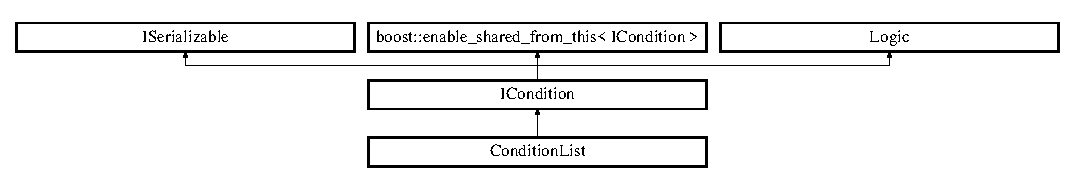
\includegraphics[height=2.014389cm]{struct_condition_list}
\end{center}
\end{figure}
\subsection*{Public Member Functions}
\begin{DoxyCompactItemize}
\item 
\mbox{\Hypertarget{struct_condition_list_a2b2cd18f8ac989cda6120ca339ae5003}\label{struct_condition_list_a2b2cd18f8ac989cda6120ca339ae5003}} 
{\bfseries R\+T\+T\+I\+\_\+\+D\+E\+CL} ()
\item 
\mbox{\Hypertarget{struct_condition_list_a2002ae78b220eac60694a784d331bee7}\label{struct_condition_list_a2002ae78b220eac60694a784d331bee7}} 
\hyperlink{struct_condition_list_a2002ae78b220eac60694a784d331bee7}{Condition\+List} ()
\begin{DoxyCompactList}\small\item\em Construction. \end{DoxyCompactList}\item 
\mbox{\Hypertarget{struct_condition_list_abe86a57fb0fe6623e86bfa7440bd5576}\label{struct_condition_list_abe86a57fb0fe6623e86bfa7440bd5576}} 
virtual void \hyperlink{struct_condition_list_abe86a57fb0fe6623e86bfa7440bd5576}{Serialize} (Json\+::\+Value \&json)
\begin{DoxyCompactList}\small\item\em I\+Serializable interface. \end{DoxyCompactList}\item 
\mbox{\Hypertarget{struct_condition_list_ae565ff13a90835d55e8453a063e1c43f}\label{struct_condition_list_ae565ff13a90835d55e8453a063e1c43f}} 
virtual void {\bfseries Deserialize} (const Json\+::\+Value \&json)
\item 
\mbox{\Hypertarget{struct_condition_list_a4b86083a53a1f1eea704c6857345661f}\label{struct_condition_list_a4b86083a53a1f1eea704c6857345661f}} 
virtual float \hyperlink{struct_condition_list_a4b86083a53a1f1eea704c6857345661f}{Test} (\hyperlink{class_goal_a818ae12a4d1f28bd433dab2a830a390e}{Goal\+::\+SP} a\+\_\+sp\+Goal)
\begin{DoxyCompactList}\small\item\em \hyperlink{class_i_condition}{I\+Condition} interface. \end{DoxyCompactList}\item 
\mbox{\Hypertarget{struct_condition_list_ae978d4a93f85cc5c0742f1d2c8608ba3}\label{struct_condition_list_ae978d4a93f85cc5c0742f1d2c8608ba3}} 
virtual \hyperlink{class_i_condition}{I\+Condition} $\ast$ \hyperlink{struct_condition_list_ae978d4a93f85cc5c0742f1d2c8608ba3}{Clone} ()
\begin{DoxyCompactList}\small\item\em Make a new instance of this \hyperlink{class_i_condition}{I\+Condition} object. \end{DoxyCompactList}\end{DoxyCompactItemize}
\subsection*{Public Attributes}
\begin{DoxyCompactItemize}
\item 
\mbox{\Hypertarget{struct_condition_list_a28d6f9b198ee583fe7ebb821e9173114}\label{struct_condition_list_a28d6f9b198ee583fe7ebb821e9173114}} 
std\+::vector$<$ \hyperlink{class_i_condition_a9e52c5b905c336e61daf97bc3f10def8}{I\+Condition\+::\+SP} $>$ {\bfseries m\+\_\+\+Conditions}
\item 
\mbox{\Hypertarget{struct_condition_list_aaa511e8de44c802040b4346ae86dc0d5}\label{struct_condition_list_aaa511e8de44c802040b4346ae86dc0d5}} 
Logical\+Op {\bfseries m\+\_\+\+Logical\+Op}
\item 
\mbox{\Hypertarget{struct_condition_list_aaf4d5d3cd39ec464341c1b752f5e3411}\label{struct_condition_list_aaf4d5d3cd39ec464341c1b752f5e3411}} 
bool {\bfseries m\+\_\+\+N\+OT}
\item 
\mbox{\Hypertarget{struct_condition_list_a9b14c5cddb657a37e5c86ff5c7500d16}\label{struct_condition_list_a9b14c5cddb657a37e5c86ff5c7500d16}} 
float {\bfseries m\+\_\+f\+Min\+True}
\end{DoxyCompactItemize}
\subsection*{Additional Inherited Members}


\subsection{Detailed Description}
This condition contains a list of conditions, it can apply a logical A\+N\+D/\+OR to the conditions, it also has a N\+OT that can be applied at the end to flip the true/false state. 

The documentation for this struct was generated from the following files\+:\begin{DoxyCompactItemize}
\item 
src/planning/conditions/Condition\+List.\+h\item 
src/planning/conditions/Condition\+List.\+cpp\end{DoxyCompactItemize}

\hypertarget{struct_config_data}{}\section{Config\+Data Struct Reference}
\label{struct_config_data}\index{Config\+Data@{Config\+Data}}
Inheritance diagram for Config\+Data\+:\begin{figure}[H]
\begin{center}
\leavevmode
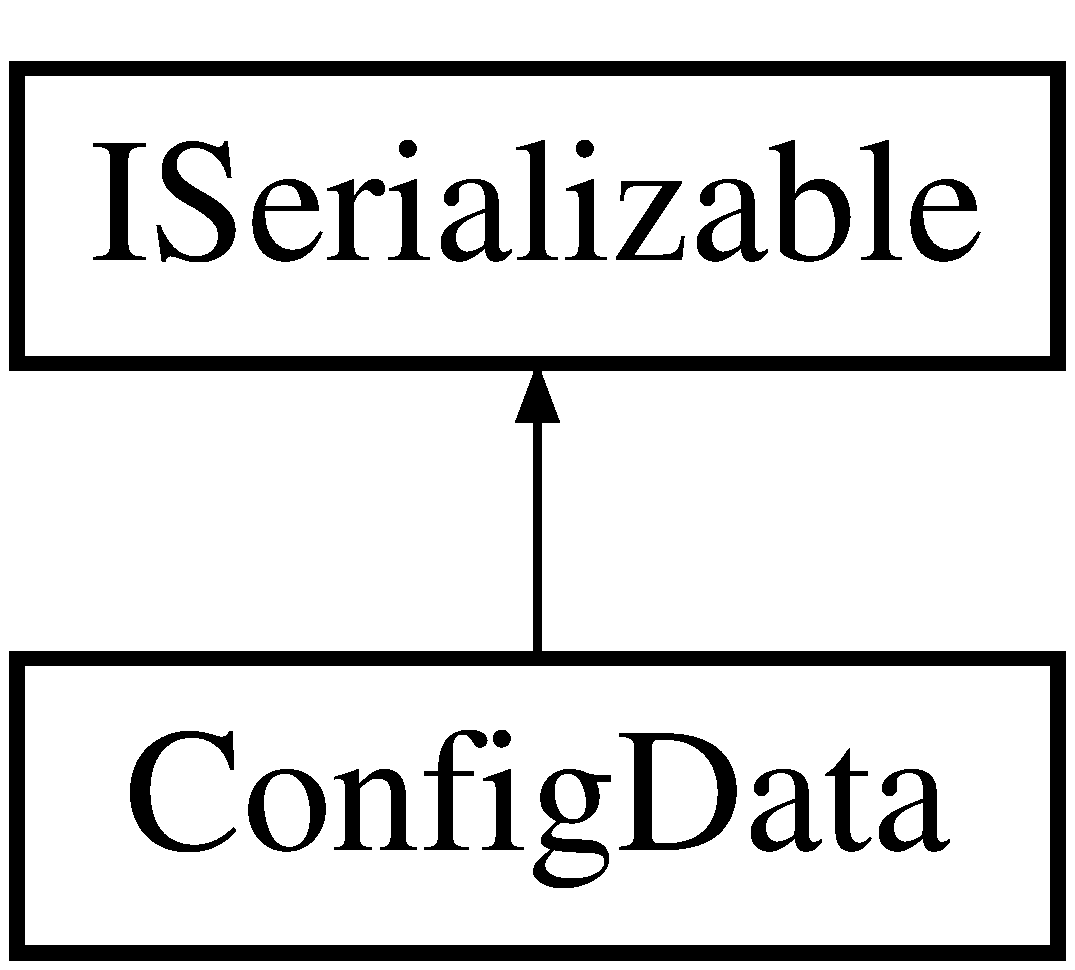
\includegraphics[height=2.000000cm]{struct_config_data}
\end{center}
\end{figure}
\subsection*{Public Member Functions}
\begin{DoxyCompactItemize}
\item 
\mbox{\Hypertarget{struct_config_data_a61f34480cd9613ec7d69ed669de35364}\label{struct_config_data_a61f34480cd9613ec7d69ed669de35364}} 
{\bfseries R\+T\+T\+I\+\_\+\+D\+E\+CL} ()
\item 
\mbox{\Hypertarget{struct_config_data_ae41cb65ae0331bdd5c2727b7169eed6f}\label{struct_config_data_ae41cb65ae0331bdd5c2727b7169eed6f}} 
virtual void {\bfseries Serialize} (Json\+::\+Value \&json)
\item 
\mbox{\Hypertarget{struct_config_data_a434b7ce05b63b7eda9503683d8d7563f}\label{struct_config_data_a434b7ce05b63b7eda9503683d8d7563f}} 
virtual void {\bfseries Deserialize} (const Json\+::\+Value \&json)
\end{DoxyCompactItemize}
\subsection*{Public Attributes}
\begin{DoxyCompactItemize}
\item 
\mbox{\Hypertarget{struct_config_data_a0358000d86f11dd0dcd8b162ad367ce9}\label{struct_config_data_a0358000d86f11dd0dcd8b162ad367ce9}} 
std\+::string {\bfseries m\+\_\+\+Dev\+Version}
\item 
\mbox{\Hypertarget{struct_config_data_a26f4ce331b58899e9fe3be62624a5476}\label{struct_config_data_a26f4ce331b58899e9fe3be62624a5476}} 
std\+::string {\bfseries m\+\_\+\+Rec\+Version}
\item 
\mbox{\Hypertarget{struct_config_data_a3eedc2fdb10342adac11a28628971930}\label{struct_config_data_a3eedc2fdb10342adac11a28628971930}} 
std\+::string {\bfseries m\+\_\+\+Req\+Version}
\end{DoxyCompactItemize}


The documentation for this struct was generated from the following file\+:\begin{DoxyCompactItemize}
\item 
src/services/\+Package\+Store/Data\+Models.\+h\end{DoxyCompactItemize}

\hypertarget{class_confirm}{}\section{Confirm Class Reference}
\label{class_confirm}\index{Confirm@{Confirm}}


{\ttfamily \#include $<$Confirm.\+h$>$}

Inheritance diagram for Confirm\+:\begin{figure}[H]
\begin{center}
\leavevmode
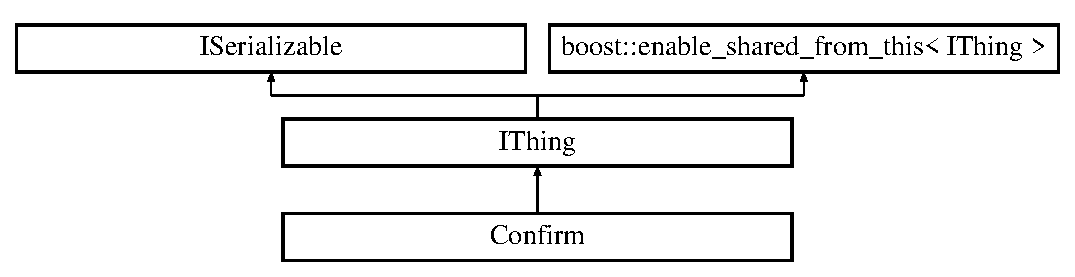
\includegraphics[height=3.000000cm]{class_confirm}
\end{center}
\end{figure}
\subsection*{Public Types}
\begin{DoxyCompactItemize}
\item 
\mbox{\Hypertarget{class_confirm_ae9623ec7393449c3dd1a867282bf934a}\label{class_confirm_ae9623ec7393449c3dd1a867282bf934a}} 
typedef boost\+::shared\+\_\+ptr$<$ \hyperlink{class_confirm}{Confirm} $>$ \hyperlink{class_confirm_ae9623ec7393449c3dd1a867282bf934a}{SP}
\begin{DoxyCompactList}\small\item\em Types. \end{DoxyCompactList}\item 
\mbox{\Hypertarget{class_confirm_abca7c131a80885546d07b112754c4703}\label{class_confirm_abca7c131a80885546d07b112754c4703}} 
typedef boost\+::weak\+\_\+ptr$<$ \hyperlink{class_confirm}{Confirm} $>$ {\bfseries WP}
\end{DoxyCompactItemize}
\subsection*{Public Member Functions}
\begin{DoxyCompactItemize}
\item 
\mbox{\Hypertarget{class_confirm_afa2c80de6f252009ba1172c1084c34b9}\label{class_confirm_afa2c80de6f252009ba1172c1084c34b9}} 
{\bfseries R\+T\+T\+I\+\_\+\+D\+E\+CL} ()
\item 
\mbox{\Hypertarget{class_confirm_ad89a0e48bd631936bcebae6797ffdb4a}\label{class_confirm_ad89a0e48bd631936bcebae6797ffdb4a}} 
virtual void \hyperlink{class_confirm_ad89a0e48bd631936bcebae6797ffdb4a}{Serialize} (Json\+::\+Value \&json)
\begin{DoxyCompactList}\small\item\em I\+Serializable interface. \end{DoxyCompactList}\item 
\mbox{\Hypertarget{class_confirm_a462316911f464637e6a4db0948d14901}\label{class_confirm_a462316911f464637e6a4db0948d14901}} 
virtual void {\bfseries Deserialize} (const Json\+::\+Value \&json)
\item 
\mbox{\Hypertarget{class_confirm_a4ecc0c660e01c48e582602e0333f8f92}\label{class_confirm_a4ecc0c660e01c48e582602e0333f8f92}} 
\hyperlink{class_confirm_a4ecc0c660e01c48e582602e0333f8f92}{Confirm} ()
\begin{DoxyCompactList}\small\item\em Construction. \end{DoxyCompactList}\item 
\mbox{\Hypertarget{class_confirm_a9231a4747138f49288ab6ad3a2c031aa}\label{class_confirm_a9231a4747138f49288ab6ad3a2c031aa}} 
{\bfseries Confirm} (const std\+::string \&a\+\_\+\+Confirm\+Type)
\item 
\mbox{\Hypertarget{class_confirm_ad1f378b2556a4b379f2801a10542536d}\label{class_confirm_ad1f378b2556a4b379f2801a10542536d}} 
{\bfseries Confirm} (const std\+::string \&a\+\_\+\+Confirm\+Type, const Json\+::\+Value \&a\+\_\+\+Info)
\item 
\mbox{\Hypertarget{class_confirm_abc920cc6480dd701fe94091306ce5463}\label{class_confirm_abc920cc6480dd701fe94091306ce5463}} 
bool {\bfseries Is\+Confirmed} () const
\item 
\mbox{\Hypertarget{class_confirm_afd38a32965e6872089a540358ec24ece}\label{class_confirm_afd38a32965e6872089a540358ec24ece}} 
const Json\+::\+Value \& {\bfseries Get\+Info} () const
\item 
\mbox{\Hypertarget{class_confirm_a745d16c0d2eb3f12204f2227c07f4789}\label{class_confirm_a745d16c0d2eb3f12204f2227c07f4789}} 
const std\+::string \& {\bfseries Get\+Confirm\+Type} () const
\item 
\mbox{\Hypertarget{class_confirm_ab24a1ed9ab498ce99abfa1c0ee515b2b}\label{class_confirm_ab24a1ed9ab498ce99abfa1c0ee515b2b}} 
void {\bfseries On\+Confirmed} ()
\item 
\mbox{\Hypertarget{class_confirm_a0d8bd7e4958ebdebcf9f1a1dff28394b}\label{class_confirm_a0d8bd7e4958ebdebcf9f1a1dff28394b}} 
void {\bfseries On\+Cancelled} ()
\end{DoxyCompactItemize}
\subsection*{Additional Inherited Members}


\subsection{Detailed Description}
This object is placed on the blackboard when we need self to confirm an action before we act. The \hyperlink{class_feedback_agent}{Feedback\+Agent} will handle the positive/negative feedback that will trigger the confirm or cancel responses of this object. 

The documentation for this class was generated from the following files\+:\begin{DoxyCompactItemize}
\item 
src/blackboard/Confirm.\+h\item 
src/blackboard/Confirm.\+cpp\end{DoxyCompactItemize}

\hypertarget{struct_rest_gesture_1_1_context}{}\section{Rest\+Gesture\+:\+:Context Struct Reference}
\label{struct_rest_gesture_1_1_context}\index{Rest\+Gesture\+::\+Context@{Rest\+Gesture\+::\+Context}}
\subsection*{Public Attributes}
\begin{DoxyCompactItemize}
\item 
\mbox{\Hypertarget{struct_rest_gesture_1_1_context_a73649aba0987583e1677af3fe4e29ff5}\label{struct_rest_gesture_1_1_context_a73649aba0987583e1677af3fe4e29ff5}} 
Gesture\+Delegate {\bfseries m\+\_\+\+Callback}
\item 
\mbox{\Hypertarget{struct_rest_gesture_1_1_context_a9d130fbb271b2f310dedc789201a90a7}\label{struct_rest_gesture_1_1_context_a9d130fbb271b2f310dedc789201a90a7}} 
\hyperlink{class_params_map}{Params\+Map} {\bfseries m\+\_\+\+Params}
\item 
\mbox{\Hypertarget{struct_rest_gesture_1_1_context_a04b21096ee5c2e3d3f28c170069f213f}\label{struct_rest_gesture_1_1_context_a04b21096ee5c2e3d3f28c170069f213f}} 
std\+::string {\bfseries m\+\_\+\+Response}
\item 
\mbox{\Hypertarget{struct_rest_gesture_1_1_context_a051a33b2e79cf21a8b097046a4ccb84a}\label{struct_rest_gesture_1_1_context_a051a33b2e79cf21a8b097046a4ccb84a}} 
bool {\bfseries m\+\_\+\+Error}
\end{DoxyCompactItemize}


The documentation for this struct was generated from the following file\+:\begin{DoxyCompactItemize}
\item 
src/gestures/Rest\+Gesture.\+h\end{DoxyCompactItemize}

\hypertarget{class_conversation_proxy}{}\section{Conversation\+Proxy Class Reference}
\label{class_conversation_proxy}\index{Conversation\+Proxy@{Conversation\+Proxy}}
Inheritance diagram for Conversation\+Proxy\+:\begin{figure}[H]
\begin{center}
\leavevmode
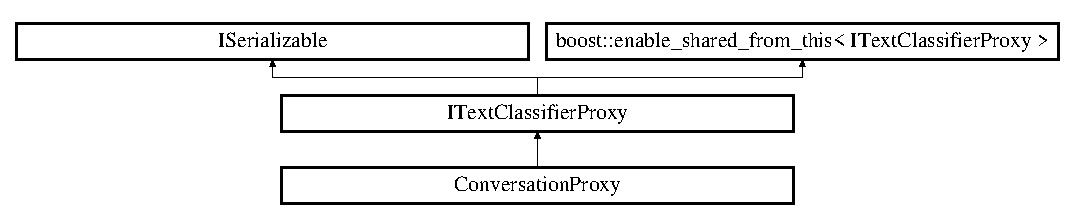
\includegraphics[height=2.514970cm]{class_conversation_proxy}
\end{center}
\end{figure}
\subsection*{Public Member Functions}
\begin{DoxyCompactItemize}
\item 
\mbox{\Hypertarget{class_conversation_proxy_a4162ffa048b1b4b9a86d8f1bac946c2b}\label{class_conversation_proxy_a4162ffa048b1b4b9a86d8f1bac946c2b}} 
{\bfseries R\+T\+T\+I\+\_\+\+D\+E\+CL} ()
\item 
\mbox{\Hypertarget{class_conversation_proxy_aad95391a2842d7862d12f1995f3cda29}\label{class_conversation_proxy_aad95391a2842d7862d12f1995f3cda29}} 
\hyperlink{class_conversation_proxy_aad95391a2842d7862d12f1995f3cda29}{Conversation\+Proxy} ()
\begin{DoxyCompactList}\small\item\em Construction. \end{DoxyCompactList}\item 
\mbox{\Hypertarget{class_conversation_proxy_a2d2a6b1626561ace7f91530b7518b3e9}\label{class_conversation_proxy_a2d2a6b1626561ace7f91530b7518b3e9}} 
virtual void \hyperlink{class_conversation_proxy_a2d2a6b1626561ace7f91530b7518b3e9}{Serialize} (Json\+::\+Value \&json)
\begin{DoxyCompactList}\small\item\em I\+Serializable interface. \end{DoxyCompactList}\item 
\mbox{\Hypertarget{class_conversation_proxy_a8c91058aa38f62f411bfb2af5ab98871}\label{class_conversation_proxy_a8c91058aa38f62f411bfb2af5ab98871}} 
virtual void {\bfseries Deserialize} (const Json\+::\+Value \&json)
\item 
\mbox{\Hypertarget{class_conversation_proxy_a482537f556269b33579dc33e22ce4bcd}\label{class_conversation_proxy_a482537f556269b33579dc33e22ce4bcd}} 
virtual void \hyperlink{class_conversation_proxy_a482537f556269b33579dc33e22ce4bcd}{Start} ()
\begin{DoxyCompactList}\small\item\em \hyperlink{class_i_text_classifier_proxy}{I\+Text\+Classifier\+Proxy} interface. \end{DoxyCompactList}\item 
\mbox{\Hypertarget{class_conversation_proxy_a33841bc367dd5971c54440416470fcb2}\label{class_conversation_proxy_a33841bc367dd5971c54440416470fcb2}} 
virtual void {\bfseries Stop} ()
\item 
\mbox{\Hypertarget{class_conversation_proxy_a93d029052ebff80dbe2886cf457dc81a}\label{class_conversation_proxy_a93d029052ebff80dbe2886cf457dc81a}} 
virtual void {\bfseries Classify\+Text} (\hyperlink{class_text_a35ce88bdca4f380b865b6066079230b1}{Text\+::\+SP} a\+\_\+sp\+Text, Delegate$<$ \hyperlink{struct_i_text_classifier_proxy_1_1_classify_result}{Classify\+Result} $\ast$$>$ a\+\_\+\+Callback)
\item 
\mbox{\Hypertarget{class_conversation_proxy_a11f23d4459907f1cee9be15ca0e25558}\label{class_conversation_proxy_a11f23d4459907f1cee9be15ca0e25558}} 
void {\bfseries On\+Emotional\+State} (const \hyperlink{class_thing_event}{Thing\+Event} \&a\+\_\+\+Thing\+Event)
\end{DoxyCompactItemize}
\subsection*{Additional Inherited Members}


The documentation for this class was generated from the following files\+:\begin{DoxyCompactItemize}
\item 
src/classifiers/proxies/Conversation\+Proxy.\+h\item 
src/classifiers/proxies/Conversation\+Proxy.\+cpp\end{DoxyCompactItemize}

\hypertarget{class_create_action}{}\section{Create\+Action Class Reference}
\label{class_create_action}\index{Create\+Action@{Create\+Action}}


{\ttfamily \#include $<$Create\+Action.\+h$>$}

Inheritance diagram for Create\+Action\+:\begin{figure}[H]
\begin{center}
\leavevmode
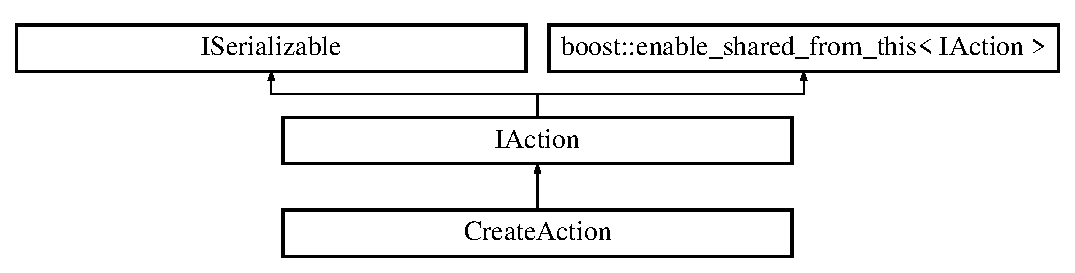
\includegraphics[height=3.000000cm]{class_create_action}
\end{center}
\end{figure}
\subsection*{Public Member Functions}
\begin{DoxyCompactItemize}
\item 
\mbox{\Hypertarget{class_create_action_af604f763d3ead8f78a4707cdd17a386c}\label{class_create_action_af604f763d3ead8f78a4707cdd17a386c}} 
{\bfseries R\+T\+T\+I\+\_\+\+D\+E\+CL} ()
\item 
\mbox{\Hypertarget{class_create_action_ace7af1feef3a0ba0b101256e74d58996}\label{class_create_action_ace7af1feef3a0ba0b101256e74d58996}} 
\hyperlink{class_create_action_ace7af1feef3a0ba0b101256e74d58996}{Create\+Action} ()
\begin{DoxyCompactList}\small\item\em Construction. \end{DoxyCompactList}\item 
\mbox{\Hypertarget{class_create_action_ad8a4b25a8c77d8e379e0f39f84a537a6}\label{class_create_action_ad8a4b25a8c77d8e379e0f39f84a537a6}} 
virtual void \hyperlink{class_create_action_ad8a4b25a8c77d8e379e0f39f84a537a6}{Serialize} (Json\+::\+Value \&json)
\begin{DoxyCompactList}\small\item\em I\+Serializable interface. \end{DoxyCompactList}\item 
\mbox{\Hypertarget{class_create_action_a3b3f5527b6ac1747927808d76f744188}\label{class_create_action_a3b3f5527b6ac1747927808d76f744188}} 
virtual void {\bfseries Deserialize} (const Json\+::\+Value \&json)
\item 
\mbox{\Hypertarget{class_create_action_ac23070e18aa583e373a9e26c7ab6d3a8}\label{class_create_action_ac23070e18aa583e373a9e26c7ab6d3a8}} 
virtual void \hyperlink{class_create_action_ac23070e18aa583e373a9e26c7ab6d3a8}{Execute} (const \hyperlink{class_goal_a818ae12a4d1f28bd433dab2a830a390e}{Goal\+::\+SP} \&a\+\_\+sp\+Goal, Delegate$<$ const \hyperlink{struct_i_action_1_1_state}{State} \&$>$ a\+\_\+\+Callback)
\begin{DoxyCompactList}\small\item\em \hyperlink{class_i_action}{I\+Action} interface. \end{DoxyCompactList}\item 
\mbox{\Hypertarget{class_create_action_a4e8abe3c1f0e767c8536a20e59c5acfa}\label{class_create_action_a4e8abe3c1f0e767c8536a20e59c5acfa}} 
virtual \hyperlink{class_i_action}{I\+Action} $\ast$ \hyperlink{class_create_action_a4e8abe3c1f0e767c8536a20e59c5acfa}{Clone} ()
\begin{DoxyCompactList}\small\item\em Make a new instance copy of this action object. \end{DoxyCompactList}\item 
\mbox{\Hypertarget{class_create_action_a815aa769367621586abbf8aa94d54c19}\label{class_create_action_a815aa769367621586abbf8aa94d54c19}} 
bool \hyperlink{class_create_action_a815aa769367621586abbf8aa94d54c19}{Attach\+To\+Root} () const
\begin{DoxyCompactList}\small\item\em Accessors. \end{DoxyCompactList}\item 
\mbox{\Hypertarget{class_create_action_a72a439a5e9a23aeded689809b5bd286d}\label{class_create_action_a72a439a5e9a23aeded689809b5bd286d}} 
float {\bfseries Get\+Importance} () const
\item 
\mbox{\Hypertarget{class_create_action_acdfa0f60401f5c09c8958d669208d1a7}\label{class_create_action_acdfa0f60401f5c09c8958d669208d1a7}} 
const \hyperlink{class_params_map}{Params\+Map} \& {\bfseries Get\+Goal\+Params} () const
\item 
\mbox{\Hypertarget{class_create_action_aed0f6d95fc1658125a4c29e05f71b95e}\label{class_create_action_aed0f6d95fc1658125a4c29e05f71b95e}} 
bool {\bfseries Get\+Replace\+Params} () const
\item 
\mbox{\Hypertarget{class_create_action_ac6274e6904fb6acd2222ed03e5a89023}\label{class_create_action_ac6274e6904fb6acd2222ed03e5a89023}} 
const std\+::string \& {\bfseries Get\+Initial\+State} () const
\item 
\mbox{\Hypertarget{class_create_action_a0ec0f7381da9b705a63d6a9c536b674a}\label{class_create_action_a0ec0f7381da9b705a63d6a9c536b674a}} 
const std\+::string \& {\bfseries Get\+Completed\+State} () const
\item 
\mbox{\Hypertarget{class_create_action_af1b9fedd8d610c9e41119823266a0ba6}\label{class_create_action_af1b9fedd8d610c9e41119823266a0ba6}} 
const std\+::string \& {\bfseries Get\+Failed\+State} () const
\item 
\mbox{\Hypertarget{class_create_action_ac63dddded3b3de271d0541afa64caf50}\label{class_create_action_ac63dddded3b3de271d0541afa64caf50}} 
void \hyperlink{class_create_action_ac63dddded3b3de271d0541afa64caf50}{Set\+Attach\+To\+Root} (bool a\+\_\+b\+Attach\+To\+Root)
\begin{DoxyCompactList}\small\item\em Mutators. \end{DoxyCompactList}\item 
\mbox{\Hypertarget{class_create_action_a490159d7be18034ee11b2faf1bda96d0}\label{class_create_action_a490159d7be18034ee11b2faf1bda96d0}} 
void {\bfseries Set\+Importance} (float a\+\_\+f\+Importance)
\item 
\mbox{\Hypertarget{class_create_action_ac45e984d2846e7584d9bc2f1a11d8b03}\label{class_create_action_ac45e984d2846e7584d9bc2f1a11d8b03}} 
\hyperlink{class_params_map}{Params\+Map} \& {\bfseries Get\+Goal\+Params} ()
\item 
\mbox{\Hypertarget{class_create_action_a7d87f0df66148df95bffd8449f64af13}\label{class_create_action_a7d87f0df66148df95bffd8449f64af13}} 
void {\bfseries Set\+Replace\+Params} (bool a\+\_\+b\+Replace)
\item 
\mbox{\Hypertarget{class_create_action_a5a25fab15f93477461590466f2fd2273}\label{class_create_action_a5a25fab15f93477461590466f2fd2273}} 
void {\bfseries Set\+Inital\+State} (const std\+::string \&a\+\_\+\+Inital\+State)
\item 
\mbox{\Hypertarget{class_create_action_a8121af05414f2f4cf26e5f4d86b68c3c}\label{class_create_action_a8121af05414f2f4cf26e5f4d86b68c3c}} 
void {\bfseries Set\+Completed\+State} (const std\+::string \&a\+\_\+\+Wait\+State)
\item 
\mbox{\Hypertarget{class_create_action_a5019cd728a3f3a59b4ff9f4719c309a7}\label{class_create_action_a5019cd728a3f3a59b4ff9f4719c309a7}} 
void {\bfseries Set\+Failed\+State} (const std\+::string \&a\+\_\+\+Failed\+State)
\end{DoxyCompactItemize}
\subsection*{Additional Inherited Members}


\subsection{Detailed Description}
This action creates a new object on the blackboard attached to the provided goal object. This action uses the \hyperlink{class_params_map}{Params\+Map} of the goal to resolve any variables into their final form then we try to deserialize an object from the provided json. 

The documentation for this class was generated from the following files\+:\begin{DoxyCompactItemize}
\item 
src/planning/actions/Create\+Action.\+h\item 
src/planning/actions/Create\+Action.\+cpp\end{DoxyCompactItemize}

\hypertarget{struct_graph_connector_1_1_create_edge_event}{}\section{Graph\+Connector\+:\+:Create\+Edge\+Event Struct Reference}
\label{struct_graph_connector_1_1_create_edge_event}\index{Graph\+Connector\+::\+Create\+Edge\+Event@{Graph\+Connector\+::\+Create\+Edge\+Event}}
Inheritance diagram for Graph\+Connector\+:\+:Create\+Edge\+Event\+:\begin{figure}[H]
\begin{center}
\leavevmode
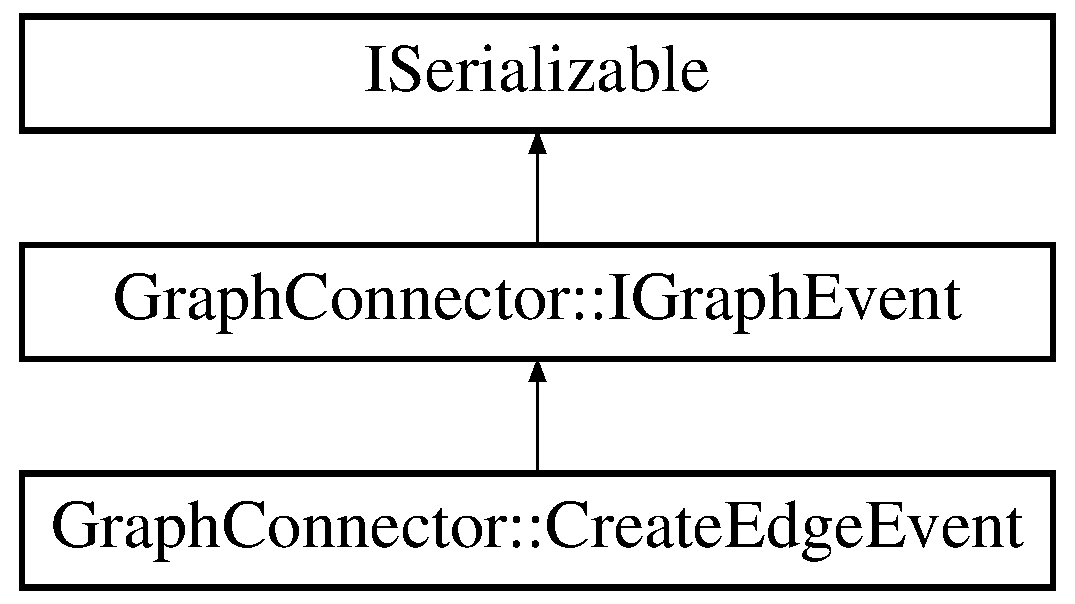
\includegraphics[height=3.000000cm]{struct_graph_connector_1_1_create_edge_event}
\end{center}
\end{figure}
\subsection*{Public Member Functions}
\begin{DoxyCompactItemize}
\item 
\mbox{\Hypertarget{struct_graph_connector_1_1_create_edge_event_a59f09d87a73f150f34782a24cc93a46c}\label{struct_graph_connector_1_1_create_edge_event_a59f09d87a73f150f34782a24cc93a46c}} 
{\bfseries R\+T\+T\+I\+\_\+\+D\+E\+CL} ()
\item 
\mbox{\Hypertarget{struct_graph_connector_1_1_create_edge_event_a297a346ae3207e20e6cb387e5be03afc}\label{struct_graph_connector_1_1_create_edge_event_a297a346ae3207e20e6cb387e5be03afc}} 
{\bfseries Create\+Edge\+Event} (const \hyperlink{class_i_graph_1_1_i_edge_adfae3ec3e377543685a06b9c5d5a776a}{I\+Edge\+::\+SP} \&a\+\_\+sp\+Edge)
\item 
\mbox{\Hypertarget{struct_graph_connector_1_1_create_edge_event_a248fe9635c43e0e52988942b2dac210b}\label{struct_graph_connector_1_1_create_edge_event_a248fe9635c43e0e52988942b2dac210b}} 
virtual void \hyperlink{struct_graph_connector_1_1_create_edge_event_a248fe9635c43e0e52988942b2dac210b}{Serialize} (Json\+::\+Value \&json)
\begin{DoxyCompactList}\small\item\em I\+Serializable interface. \end{DoxyCompactList}\item 
\mbox{\Hypertarget{struct_graph_connector_1_1_create_edge_event_a9c00b46a08f0b77e0119b549175d95e5}\label{struct_graph_connector_1_1_create_edge_event_a9c00b46a08f0b77e0119b549175d95e5}} 
virtual void {\bfseries Deserialize} (const Json\+::\+Value \&json)
\item 
\mbox{\Hypertarget{struct_graph_connector_1_1_create_edge_event_a38ec62cdd25c5877f530123117a30cc7}\label{struct_graph_connector_1_1_create_edge_event_a38ec62cdd25c5877f530123117a30cc7}} 
virtual void \hyperlink{struct_graph_connector_1_1_create_edge_event_a38ec62cdd25c5877f530123117a30cc7}{Execute} ()
\begin{DoxyCompactList}\small\item\em \hyperlink{struct_graph_connector_1_1_i_graph_event}{I\+Graph\+Event} interface. \end{DoxyCompactList}\end{DoxyCompactItemize}
\subsection*{Public Attributes}
\begin{DoxyCompactItemize}
\item 
\mbox{\Hypertarget{struct_graph_connector_1_1_create_edge_event_a0d24372d11ddad5942b226ac850b2b04}\label{struct_graph_connector_1_1_create_edge_event_a0d24372d11ddad5942b226ac850b2b04}} 
\hyperlink{class_i_graph_1_1_i_edge_adfae3ec3e377543685a06b9c5d5a776a}{I\+Edge\+::\+SP} \hyperlink{struct_graph_connector_1_1_create_edge_event_a0d24372d11ddad5942b226ac850b2b04}{m\+\_\+sp\+Edge}
\begin{DoxyCompactList}\small\item\em Data. \end{DoxyCompactList}\item 
\mbox{\Hypertarget{struct_graph_connector_1_1_create_edge_event_a0c9c1793d52cf5817a03bd5834a937d1}\label{struct_graph_connector_1_1_create_edge_event_a0c9c1793d52cf5817a03bd5834a937d1}} 
std\+::string {\bfseries m\+\_\+\+Src\+Hash\+Id}
\item 
\mbox{\Hypertarget{struct_graph_connector_1_1_create_edge_event_a98a5288177d64a26e0ab6b9e6d114cdd}\label{struct_graph_connector_1_1_create_edge_event_a98a5288177d64a26e0ab6b9e6d114cdd}} 
std\+::string {\bfseries m\+\_\+\+Dst\+Hash\+Id}
\end{DoxyCompactItemize}
\subsection*{Additional Inherited Members}


The documentation for this struct was generated from the following files\+:\begin{DoxyCompactItemize}
\item 
src/models/Graph\+Connector.\+h\item 
src/models/Graph\+Connector.\+cpp\end{DoxyCompactItemize}

\hypertarget{struct_graph_connector_1_1_create_vert_event}{}\section{Graph\+Connector\+:\+:Create\+Vert\+Event Struct Reference}
\label{struct_graph_connector_1_1_create_vert_event}\index{Graph\+Connector\+::\+Create\+Vert\+Event@{Graph\+Connector\+::\+Create\+Vert\+Event}}


This is sent to the parent graph when a vertex is created.  




{\ttfamily \#include $<$Graph\+Connector.\+h$>$}

Inheritance diagram for Graph\+Connector\+:\+:Create\+Vert\+Event\+:\begin{figure}[H]
\begin{center}
\leavevmode
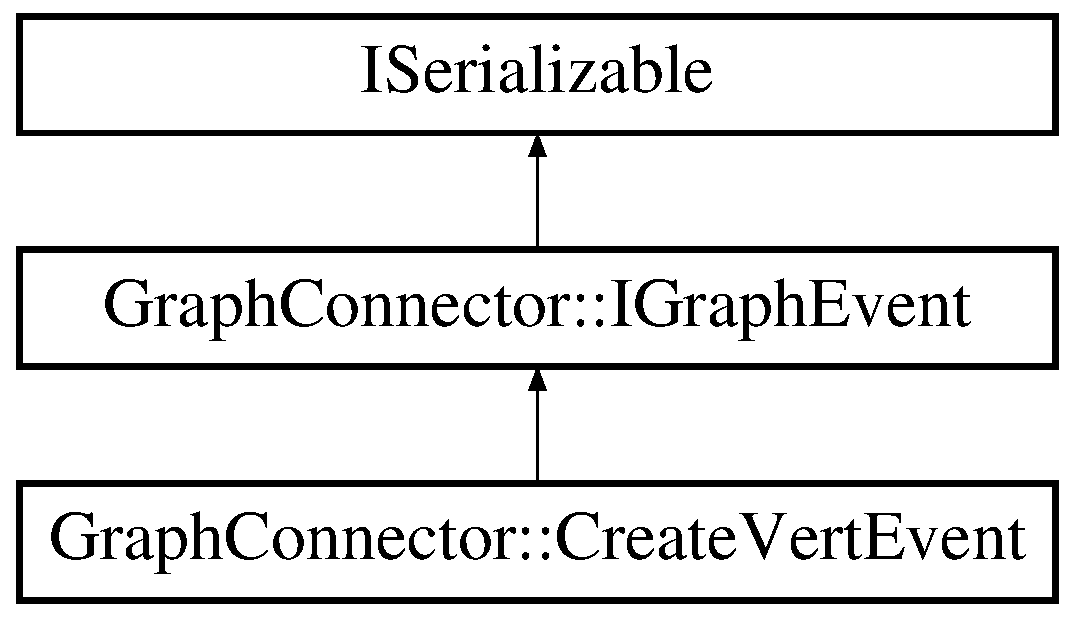
\includegraphics[height=3.000000cm]{struct_graph_connector_1_1_create_vert_event}
\end{center}
\end{figure}
\subsection*{Public Member Functions}
\begin{DoxyCompactItemize}
\item 
\mbox{\Hypertarget{struct_graph_connector_1_1_create_vert_event_a299ee4be78d6f00220734127fe9491d9}\label{struct_graph_connector_1_1_create_vert_event_a299ee4be78d6f00220734127fe9491d9}} 
{\bfseries R\+T\+T\+I\+\_\+\+D\+E\+CL} ()
\item 
\mbox{\Hypertarget{struct_graph_connector_1_1_create_vert_event_a3c84efd555873ae330ed4adc95bb925d}\label{struct_graph_connector_1_1_create_vert_event_a3c84efd555873ae330ed4adc95bb925d}} 
{\bfseries Create\+Vert\+Event} (const \hyperlink{class_i_graph_1_1_i_vertex_af72b9df91f110bc7824c608c10cc819c}{I\+Vertex\+::\+SP} \&a\+\_\+sp\+Vert)
\item 
\mbox{\Hypertarget{struct_graph_connector_1_1_create_vert_event_a681f1ef0c45f90a64696a190fe8826f8}\label{struct_graph_connector_1_1_create_vert_event_a681f1ef0c45f90a64696a190fe8826f8}} 
virtual void \hyperlink{struct_graph_connector_1_1_create_vert_event_a681f1ef0c45f90a64696a190fe8826f8}{Serialize} (Json\+::\+Value \&json)
\begin{DoxyCompactList}\small\item\em I\+Serializable interface. \end{DoxyCompactList}\item 
\mbox{\Hypertarget{struct_graph_connector_1_1_create_vert_event_a129fa594e912d2c4b9c918843577a19a}\label{struct_graph_connector_1_1_create_vert_event_a129fa594e912d2c4b9c918843577a19a}} 
virtual void {\bfseries Deserialize} (const Json\+::\+Value \&json)
\item 
\mbox{\Hypertarget{struct_graph_connector_1_1_create_vert_event_a065f2f224e45404265730cbe7914c91b}\label{struct_graph_connector_1_1_create_vert_event_a065f2f224e45404265730cbe7914c91b}} 
virtual void \hyperlink{struct_graph_connector_1_1_create_vert_event_a065f2f224e45404265730cbe7914c91b}{Execute} ()
\begin{DoxyCompactList}\small\item\em \hyperlink{struct_graph_connector_1_1_i_graph_event}{I\+Graph\+Event} interface. \end{DoxyCompactList}\end{DoxyCompactItemize}
\subsection*{Public Attributes}
\begin{DoxyCompactItemize}
\item 
\mbox{\Hypertarget{struct_graph_connector_1_1_create_vert_event_a4ff17f8d2d72e9d853b8ab104314b207}\label{struct_graph_connector_1_1_create_vert_event_a4ff17f8d2d72e9d853b8ab104314b207}} 
\hyperlink{class_i_graph_1_1_i_vertex_af72b9df91f110bc7824c608c10cc819c}{I\+Vertex\+::\+SP} \hyperlink{struct_graph_connector_1_1_create_vert_event_a4ff17f8d2d72e9d853b8ab104314b207}{m\+\_\+sp\+Vert}
\begin{DoxyCompactList}\small\item\em Data. \end{DoxyCompactList}\end{DoxyCompactItemize}
\subsection*{Additional Inherited Members}


\subsection{Detailed Description}
This is sent to the parent graph when a vertex is created. 

The documentation for this struct was generated from the following files\+:\begin{DoxyCompactItemize}
\item 
src/models/Graph\+Connector.\+h\item 
src/models/Graph\+Connector.\+cpp\end{DoxyCompactItemize}

\hypertarget{class_data_store_s_q_l_l}{}\section{Data\+Store\+S\+Q\+LL Class Reference}
\label{class_data_store_s_q_l_l}\index{Data\+Store\+S\+Q\+LL@{Data\+Store\+S\+Q\+LL}}
Inheritance diagram for Data\+Store\+S\+Q\+LL\+:\begin{figure}[H]
\begin{center}
\leavevmode
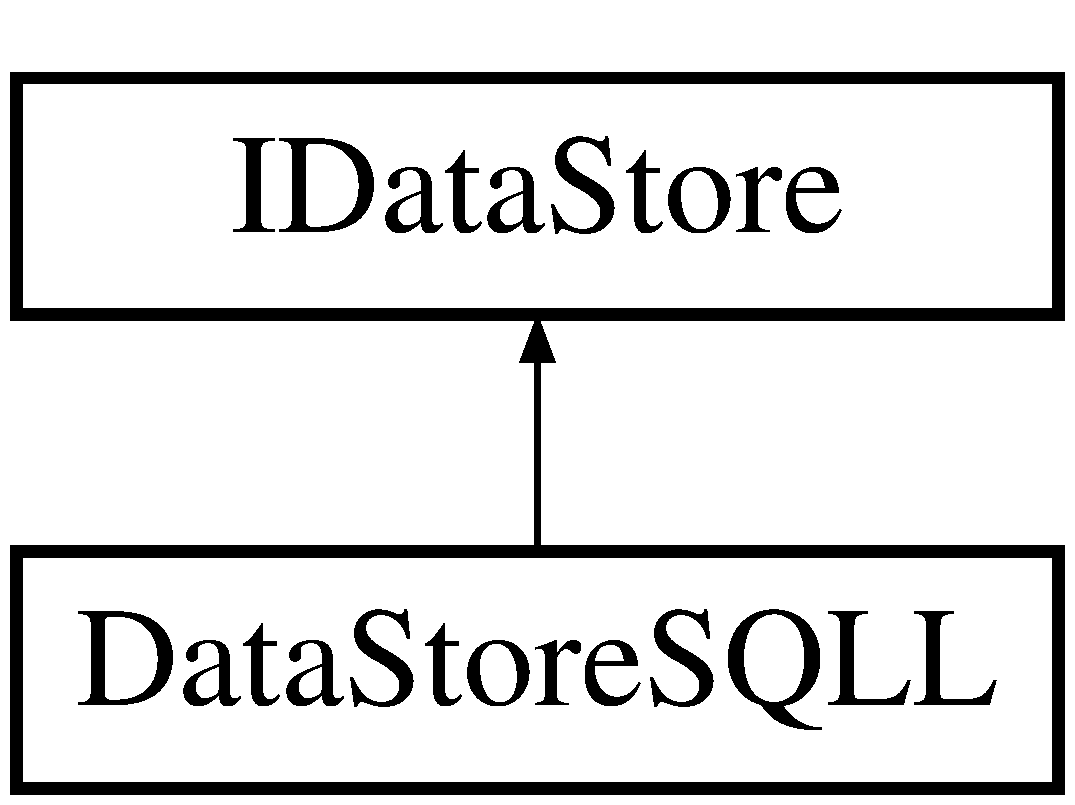
\includegraphics[height=2.000000cm]{class_data_store_s_q_l_l}
\end{center}
\end{figure}
\subsection*{Public Member Functions}
\begin{DoxyCompactItemize}
\item 
\mbox{\Hypertarget{class_data_store_s_q_l_l_ad362cb6a735634589de18259bc767316}\label{class_data_store_s_q_l_l_ad362cb6a735634589de18259bc767316}} 
{\bfseries R\+T\+T\+I\+\_\+\+D\+E\+CL} ()
\item 
\mbox{\Hypertarget{class_data_store_s_q_l_l_ab31e3a263ca49fe6761ec63760e15809}\label{class_data_store_s_q_l_l_ab31e3a263ca49fe6761ec63760e15809}} 
\hyperlink{class_data_store_s_q_l_l_ab31e3a263ca49fe6761ec63760e15809}{Data\+Store\+S\+Q\+LL} ()
\begin{DoxyCompactList}\small\item\em C\+Onstruction. \end{DoxyCompactList}\item 
\mbox{\Hypertarget{class_data_store_s_q_l_l_a2cd1693fa646f2aaf9a0d083263fc567}\label{class_data_store_s_q_l_l_a2cd1693fa646f2aaf9a0d083263fc567}} 
virtual bool \hyperlink{class_data_store_s_q_l_l_a2cd1693fa646f2aaf9a0d083263fc567}{Start} (const std\+::string \&a\+\_\+\+DB, const Json\+::\+Value \&a\+\_\+\+Data\+Definition)
\begin{DoxyCompactList}\small\item\em \hyperlink{class_i_data_store}{I\+Data\+Store} interface. \end{DoxyCompactList}\item 
\mbox{\Hypertarget{class_data_store_s_q_l_l_ae31fe0b15e58cb23ae928267ef3e72ad}\label{class_data_store_s_q_l_l_ae31fe0b15e58cb23ae928267ef3e72ad}} 
virtual bool \hyperlink{class_data_store_s_q_l_l_ae31fe0b15e58cb23ae928267ef3e72ad}{Stop} ()
\begin{DoxyCompactList}\small\item\em Shutdown this data store, any pending data should be flushed. \end{DoxyCompactList}\item 
\mbox{\Hypertarget{class_data_store_s_q_l_l_aa7f301e01cd51702d395064c3ec8a9f3}\label{class_data_store_s_q_l_l_aa7f301e01cd51702d395064c3ec8a9f3}} 
virtual bool \hyperlink{class_data_store_s_q_l_l_aa7f301e01cd51702d395064c3ec8a9f3}{Save} (const std\+::string \&a\+\_\+\+ID, const Json\+::\+Value \&a\+\_\+\+Data, Delegate$<$ bool $>$ a\+\_\+\+Callback=Delegate$<$ bool $>$())
\begin{DoxyCompactList}\small\item\em Store data into this data store. \end{DoxyCompactList}\item 
\mbox{\Hypertarget{class_data_store_s_q_l_l_ae041df984085331486d97ba819adb896}\label{class_data_store_s_q_l_l_ae041df984085331486d97ba819adb896}} 
virtual bool \hyperlink{class_data_store_s_q_l_l_ae041df984085331486d97ba819adb896}{Load} (const std\+::string \&a\+\_\+\+ID, Delegate$<$ Json\+::\+Value $\ast$$>$ a\+\_\+\+Callback)
\begin{DoxyCompactList}\small\item\em Get data from this store by it\textquotesingle{}s primary ID, this is asynchronous and will invoke the callback. \end{DoxyCompactList}\item 
\mbox{\Hypertarget{class_data_store_s_q_l_l_a1a8cbf495f74cfb43ed9d46bc9cc91cb}\label{class_data_store_s_q_l_l_a1a8cbf495f74cfb43ed9d46bc9cc91cb}} 
virtual bool \hyperlink{class_data_store_s_q_l_l_a1a8cbf495f74cfb43ed9d46bc9cc91cb}{Delete} (const std\+::string \&a\+\_\+\+ID, Delegate$<$ bool $>$ a\+\_\+\+Callback=Delegate$<$ bool $>$())
\begin{DoxyCompactList}\small\item\em Delete data from this store by it\textquotesingle{}s primary ID. \end{DoxyCompactList}\item 
virtual bool \hyperlink{class_data_store_s_q_l_l_ad2da91d2589839e6e02d3030c9fd832d}{Find} (const Conditions \&a\+\_\+\+Conditions, Delegate$<$ Query\+Results $\ast$$>$ a\+\_\+\+Callback)
\end{DoxyCompactItemize}
\subsection*{Additional Inherited Members}


\subsection{Member Function Documentation}
\mbox{\Hypertarget{class_data_store_s_q_l_l_ad2da91d2589839e6e02d3030c9fd832d}\label{class_data_store_s_q_l_l_ad2da91d2589839e6e02d3030c9fd832d}} 
\index{Data\+Store\+S\+Q\+LL@{Data\+Store\+S\+Q\+LL}!Find@{Find}}
\index{Find@{Find}!Data\+Store\+S\+Q\+LL@{Data\+Store\+S\+Q\+LL}}
\subsubsection{\texorpdfstring{Find()}{Find()}}
{\footnotesize\ttfamily bool Data\+Store\+S\+Q\+L\+L\+::\+Find (\begin{DoxyParamCaption}\item[{const Conditions \&}]{a\+\_\+\+Conditions,  }\item[{Delegate$<$ Query\+Results $\ast$$>$}]{a\+\_\+\+Callback }\end{DoxyParamCaption})\hspace{0.3cm}{\ttfamily [virtual]}}

Query for data based on conditions, this will invoke your callback with the ID\textquotesingle{}s of all records that match your conditions. 

Implements \hyperlink{class_i_data_store_aa3e9e7b57b40b3c7ff2bd11c9f9b9bf7}{I\+Data\+Store}.



The documentation for this class was generated from the following files\+:\begin{DoxyCompactItemize}
\item 
src/utils/Data\+Store\+S\+Q\+L\+L.\+h\item 
src/utils/Data\+Store\+S\+Q\+L\+L.\+cpp\end{DoxyCompactItemize}

\hypertarget{class_deep_q_a}{}\section{Deep\+QA Class Reference}
\label{class_deep_q_a}\index{Deep\+QA@{Deep\+QA}}
Inheritance diagram for Deep\+QA\+:\begin{figure}[H]
\begin{center}
\leavevmode
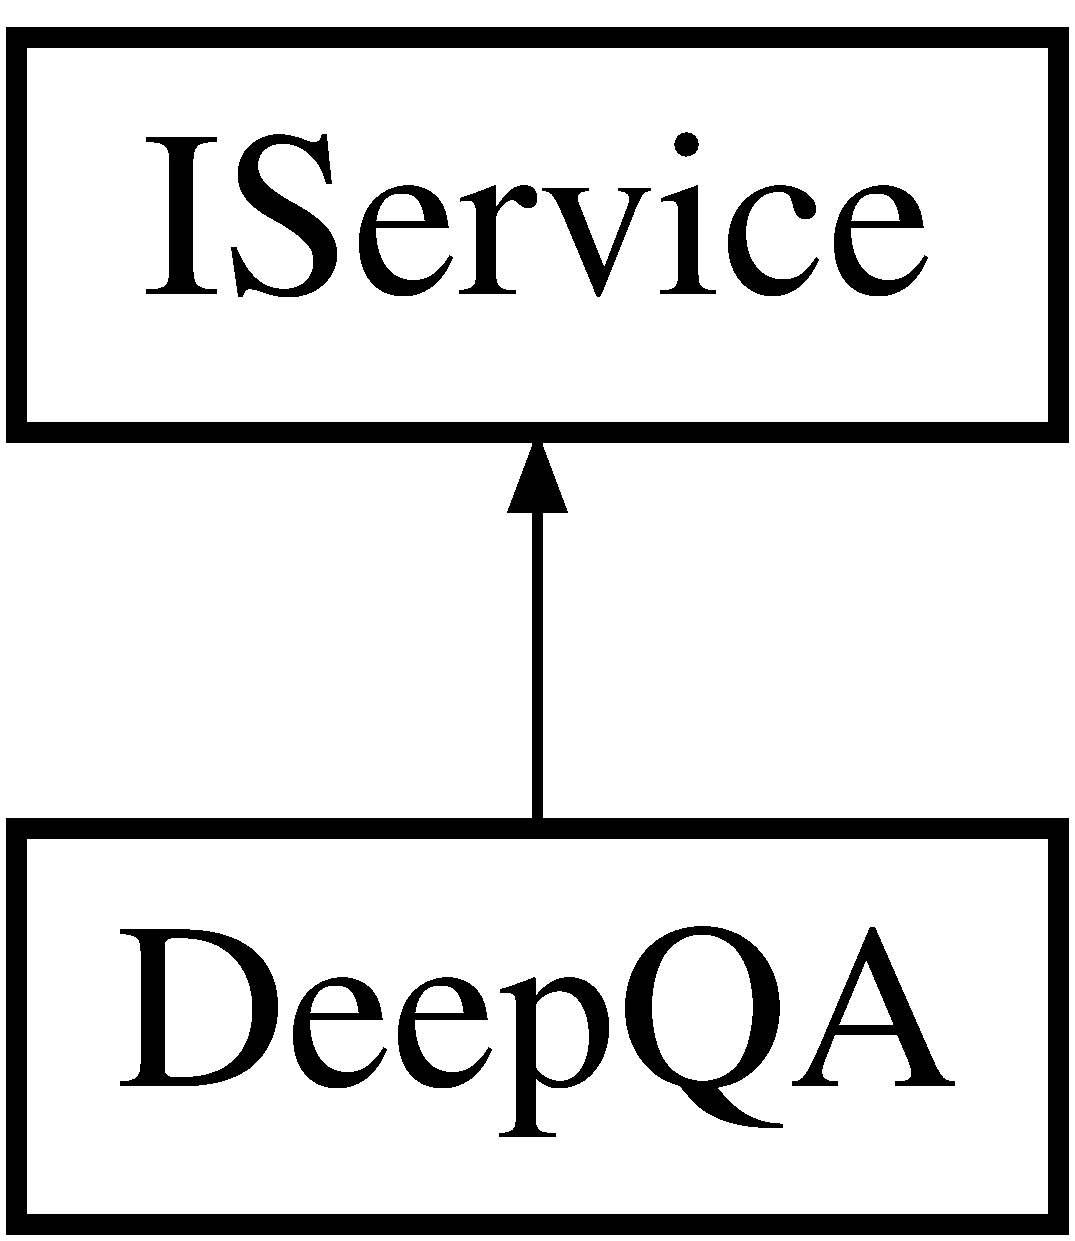
\includegraphics[height=2.000000cm]{class_deep_q_a}
\end{center}
\end{figure}
\subsection*{Public Member Functions}
\begin{DoxyCompactItemize}
\item 
\mbox{\Hypertarget{class_deep_q_a_af102560fa1f99a45eae69b5743c89f37}\label{class_deep_q_a_af102560fa1f99a45eae69b5743c89f37}} 
{\bfseries R\+T\+T\+I\+\_\+\+D\+E\+CL} ()
\item 
\mbox{\Hypertarget{class_deep_q_a_ae089062a354214cd8b3885782994c8de}\label{class_deep_q_a_ae089062a354214cd8b3885782994c8de}} 
\hyperlink{class_deep_q_a_ae089062a354214cd8b3885782994c8de}{Deep\+QA} ()
\begin{DoxyCompactList}\small\item\em Construction. \end{DoxyCompactList}\item 
\mbox{\Hypertarget{class_deep_q_a_afa355c4f57b2fa096703721857dafbeb}\label{class_deep_q_a_afa355c4f57b2fa096703721857dafbeb}} 
virtual void \hyperlink{class_deep_q_a_afa355c4f57b2fa096703721857dafbeb}{Serialize} (Json\+::\+Value \&json)
\begin{DoxyCompactList}\small\item\em I\+Serializable. \end{DoxyCompactList}\item 
\mbox{\Hypertarget{class_deep_q_a_a9d63f6c4ac86c0f5ef5f833ff45b9a87}\label{class_deep_q_a_a9d63f6c4ac86c0f5ef5f833ff45b9a87}} 
virtual void {\bfseries Deserialize} (const Json\+::\+Value \&json)
\item 
\mbox{\Hypertarget{class_deep_q_a_a8382e328037e716bff5043658e1d97e6}\label{class_deep_q_a_a8382e328037e716bff5043658e1d97e6}} 
virtual bool \hyperlink{class_deep_q_a_a8382e328037e716bff5043658e1d97e6}{Start} ()
\begin{DoxyCompactList}\small\item\em I\+Service interface. \end{DoxyCompactList}\item 
\mbox{\Hypertarget{class_deep_q_a_ab82a3d90e8f0c1f2431219e235f7c26e}\label{class_deep_q_a_ab82a3d90e8f0c1f2431219e235f7c26e}} 
void {\bfseries Ask\+Question} (const std\+::string \&a\+\_\+\+Input, Delegate$<$ const Json\+::\+Value \&$>$ a\+\_\+\+Callback, int a\+\_\+\+Num\+Answers=1, bool a\+\_\+b\+Infer\+Question=false, Json\+::\+Value a\+\_\+\+Evidence=Json\+::\+Value())
\end{DoxyCompactItemize}


The documentation for this class was generated from the following files\+:\begin{DoxyCompactItemize}
\item 
src/services/\+Deep\+Q\+A/Deep\+Q\+A.\+h\item 
src/services/\+Deep\+Q\+A/Deep\+Q\+A.\+cpp\end{DoxyCompactItemize}

\hypertarget{class_deep_q_a_proxy}{}\section{Deep\+Q\+A\+Proxy Class Reference}
\label{class_deep_q_a_proxy}\index{Deep\+Q\+A\+Proxy@{Deep\+Q\+A\+Proxy}}
Inheritance diagram for Deep\+Q\+A\+Proxy\+:\begin{figure}[H]
\begin{center}
\leavevmode
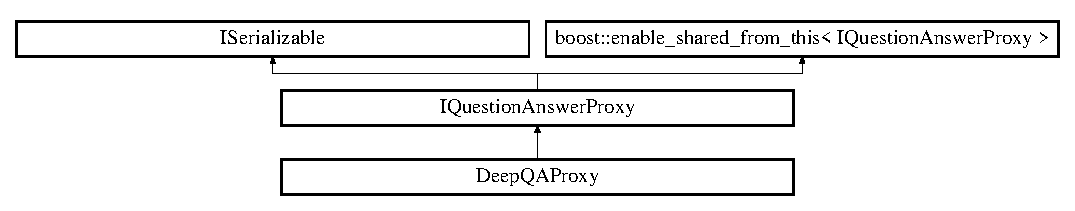
\includegraphics[height=2.393162cm]{class_deep_q_a_proxy}
\end{center}
\end{figure}
\subsection*{Public Member Functions}
\begin{DoxyCompactItemize}
\item 
\mbox{\Hypertarget{class_deep_q_a_proxy_a634e97df15d4b8e48ee1aa3328789fe6}\label{class_deep_q_a_proxy_a634e97df15d4b8e48ee1aa3328789fe6}} 
{\bfseries R\+T\+T\+I\+\_\+\+D\+E\+CL} ()
\item 
\mbox{\Hypertarget{class_deep_q_a_proxy_a7eb78b501443befd602402614986f5b6}\label{class_deep_q_a_proxy_a7eb78b501443befd602402614986f5b6}} 
\hyperlink{class_deep_q_a_proxy_a7eb78b501443befd602402614986f5b6}{Deep\+Q\+A\+Proxy} ()
\begin{DoxyCompactList}\small\item\em Construction. \end{DoxyCompactList}\item 
\mbox{\Hypertarget{class_deep_q_a_proxy_acfc85518670462ff4c2a10a974262ffc}\label{class_deep_q_a_proxy_acfc85518670462ff4c2a10a974262ffc}} 
virtual void \hyperlink{class_deep_q_a_proxy_acfc85518670462ff4c2a10a974262ffc}{Serialize} (Json\+::\+Value \&json)
\begin{DoxyCompactList}\small\item\em I\+Serializable. \end{DoxyCompactList}\item 
\mbox{\Hypertarget{class_deep_q_a_proxy_a9e02e288c8ad1c338bca7414e28168b7}\label{class_deep_q_a_proxy_a9e02e288c8ad1c338bca7414e28168b7}} 
virtual void {\bfseries Deserialize} (const Json\+::\+Value \&json)
\item 
\mbox{\Hypertarget{class_deep_q_a_proxy_acc2e8ddf79de3d7d26e5f741247427c9}\label{class_deep_q_a_proxy_acc2e8ddf79de3d7d26e5f741247427c9}} 
virtual void \hyperlink{class_deep_q_a_proxy_acc2e8ddf79de3d7d26e5f741247427c9}{Start} ()
\begin{DoxyCompactList}\small\item\em I\+Question\+Answer. \end{DoxyCompactList}\item 
\mbox{\Hypertarget{class_deep_q_a_proxy_a83687a3cee183761323ec521f66c816e}\label{class_deep_q_a_proxy_a83687a3cee183761323ec521f66c816e}} 
virtual void {\bfseries Stop} ()
\item 
\mbox{\Hypertarget{class_deep_q_a_proxy_aa922a952efa963f782311cce4bc70b89}\label{class_deep_q_a_proxy_aa922a952efa963f782311cce4bc70b89}} 
virtual void \hyperlink{class_deep_q_a_proxy_aa922a952efa963f782311cce4bc70b89}{Ask\+Question} (\hyperlink{class_question_intent_a250dceb08e1342574a0aca4fe40a7121}{Question\+Intent\+::\+SP} a\+\_\+sp\+Question, Delegate$<$ const Json\+::\+Value \&$>$ a\+\_\+\+Callback)
\begin{DoxyCompactList}\small\item\em I\+Question\+Answer. \end{DoxyCompactList}\end{DoxyCompactItemize}
\subsection*{Additional Inherited Members}


The documentation for this class was generated from the following files\+:\begin{DoxyCompactItemize}
\item 
src/agent/proxies/Deep\+Q\+A\+Proxy.\+h\item 
src/agent/proxies/Deep\+Q\+A\+Proxy.\+cpp\end{DoxyCompactItemize}

\hypertarget{class_depth_camera}{}\section{Depth\+Camera Class Reference}
\label{class_depth_camera}\index{Depth\+Camera@{Depth\+Camera}}


Base class for a 3\+D\+Camera sensor class that collects \hyperlink{class_video_data}{Video\+Data}. This is not a actual implementation, see Nao\+Camera.  




{\ttfamily \#include $<$Depth\+Camera.\+h$>$}

Inheritance diagram for Depth\+Camera\+:\begin{figure}[H]
\begin{center}
\leavevmode
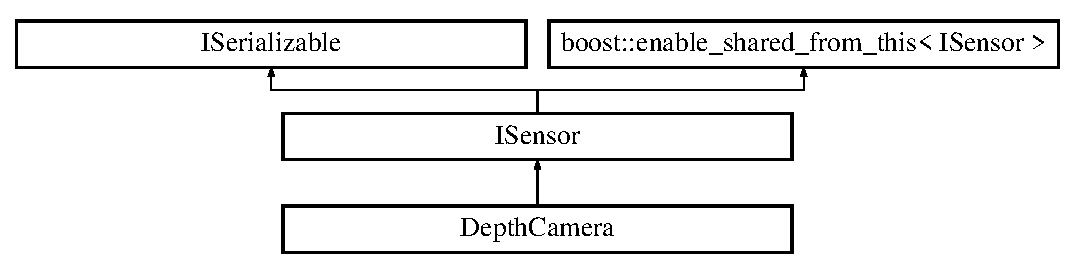
\includegraphics[height=3.000000cm]{class_depth_camera}
\end{center}
\end{figure}
\subsection*{Public Member Functions}
\begin{DoxyCompactItemize}
\item 
\mbox{\Hypertarget{class_depth_camera_a65ba6b900f13d75408d1fbb90e2b1b01}\label{class_depth_camera_a65ba6b900f13d75408d1fbb90e2b1b01}} 
{\bfseries R\+T\+T\+I\+\_\+\+D\+E\+CL} ()
\item 
\mbox{\Hypertarget{class_depth_camera_a70f1c1dca8591622d6c92dfde5d5c4e4}\label{class_depth_camera_a70f1c1dca8591622d6c92dfde5d5c4e4}} 
virtual void \hyperlink{class_depth_camera_a70f1c1dca8591622d6c92dfde5d5c4e4}{Serialize} (Json\+::\+Value \&json)
\begin{DoxyCompactList}\small\item\em I\+Serialiazable interface. \end{DoxyCompactList}\item 
\mbox{\Hypertarget{class_depth_camera_aafde1d8d16bf2dd14c303729929df0cc}\label{class_depth_camera_aafde1d8d16bf2dd14c303729929df0cc}} 
virtual void {\bfseries Deserialize} (const Json\+::\+Value \&json)
\item 
\mbox{\Hypertarget{class_depth_camera_aadd17c5e675559f14c42663902fd10e6}\label{class_depth_camera_aadd17c5e675559f14c42663902fd10e6}} 
virtual const char $\ast$ \hyperlink{class_depth_camera_aadd17c5e675559f14c42663902fd10e6}{Get\+Sensor\+Name} ()
\begin{DoxyCompactList}\small\item\em \hyperlink{class_i_sensor}{I\+Sensor} interface. \end{DoxyCompactList}\item 
\mbox{\Hypertarget{class_depth_camera_ac05b35efb90d7beace0cd8bb9c22064c}\label{class_depth_camera_ac05b35efb90d7beace0cd8bb9c22064c}} 
virtual const char $\ast$ {\bfseries Get\+Data\+Type} ()
\item 
\mbox{\Hypertarget{class_depth_camera_a6374182e6de29c0920e54779f9d12be0}\label{class_depth_camera_a6374182e6de29c0920e54779f9d12be0}} 
virtual bool \hyperlink{class_depth_camera_a6374182e6de29c0920e54779f9d12be0}{On\+Start} ()
\begin{DoxyCompactList}\small\item\em This is invoked when the first subscriber subscribes to this sensor. \end{DoxyCompactList}\item 
\mbox{\Hypertarget{class_depth_camera_a9a1f1276865887d32898f6e97dfaffea}\label{class_depth_camera_a9a1f1276865887d32898f6e97dfaffea}} 
virtual bool \hyperlink{class_depth_camera_a9a1f1276865887d32898f6e97dfaffea}{On\+Stop} ()
\begin{DoxyCompactList}\small\item\em This is invoked when the last subscriber un-\/subscribes. \end{DoxyCompactList}\item 
\mbox{\Hypertarget{class_depth_camera_a1f4ab0e4b2393ad90f6bb4767cbad31c}\label{class_depth_camera_a1f4ab0e4b2393ad90f6bb4767cbad31c}} 
virtual void \hyperlink{class_depth_camera_a1f4ab0e4b2393ad90f6bb4767cbad31c}{On\+Pause} ()
\begin{DoxyCompactList}\small\item\em This is invoked to pause this sensor. \end{DoxyCompactList}\item 
\mbox{\Hypertarget{class_depth_camera_aaf54e1c596148f5faa99b5c5dbf4daaa}\label{class_depth_camera_aaf54e1c596148f5faa99b5c5dbf4daaa}} 
virtual void \hyperlink{class_depth_camera_aaf54e1c596148f5faa99b5c5dbf4daaa}{On\+Resume} ()
\begin{DoxyCompactList}\small\item\em This is invoked to restart this sensor. \end{DoxyCompactList}\end{DoxyCompactItemize}
\subsection*{Protected Attributes}
\begin{DoxyCompactItemize}
\item 
\mbox{\Hypertarget{class_depth_camera_a333d874d5b7ec662da4955fd923a3329}\label{class_depth_camera_a333d874d5b7ec662da4955fd923a3329}} 
float \hyperlink{class_depth_camera_a333d874d5b7ec662da4955fd923a3329}{m\+\_\+f\+Frames\+Per\+Sec}
\begin{DoxyCompactList}\small\item\em Data. \end{DoxyCompactList}\end{DoxyCompactItemize}
\subsection*{Additional Inherited Members}


\subsection{Detailed Description}
Base class for a 3\+D\+Camera sensor class that collects \hyperlink{class_video_data}{Video\+Data}. This is not a actual implementation, see Nao\+Camera. 

The documentation for this class was generated from the following files\+:\begin{DoxyCompactItemize}
\item 
src/sensors/Depth\+Camera.\+h\item 
src/sensors/Depth\+Camera.\+cpp\end{DoxyCompactItemize}

\hypertarget{class_depth_video_data}{}\section{Depth\+Video\+Data Class Reference}
\label{class_depth_video_data}\index{Depth\+Video\+Data@{Depth\+Video\+Data}}
Inheritance diagram for Depth\+Video\+Data\+:\begin{figure}[H]
\begin{center}
\leavevmode
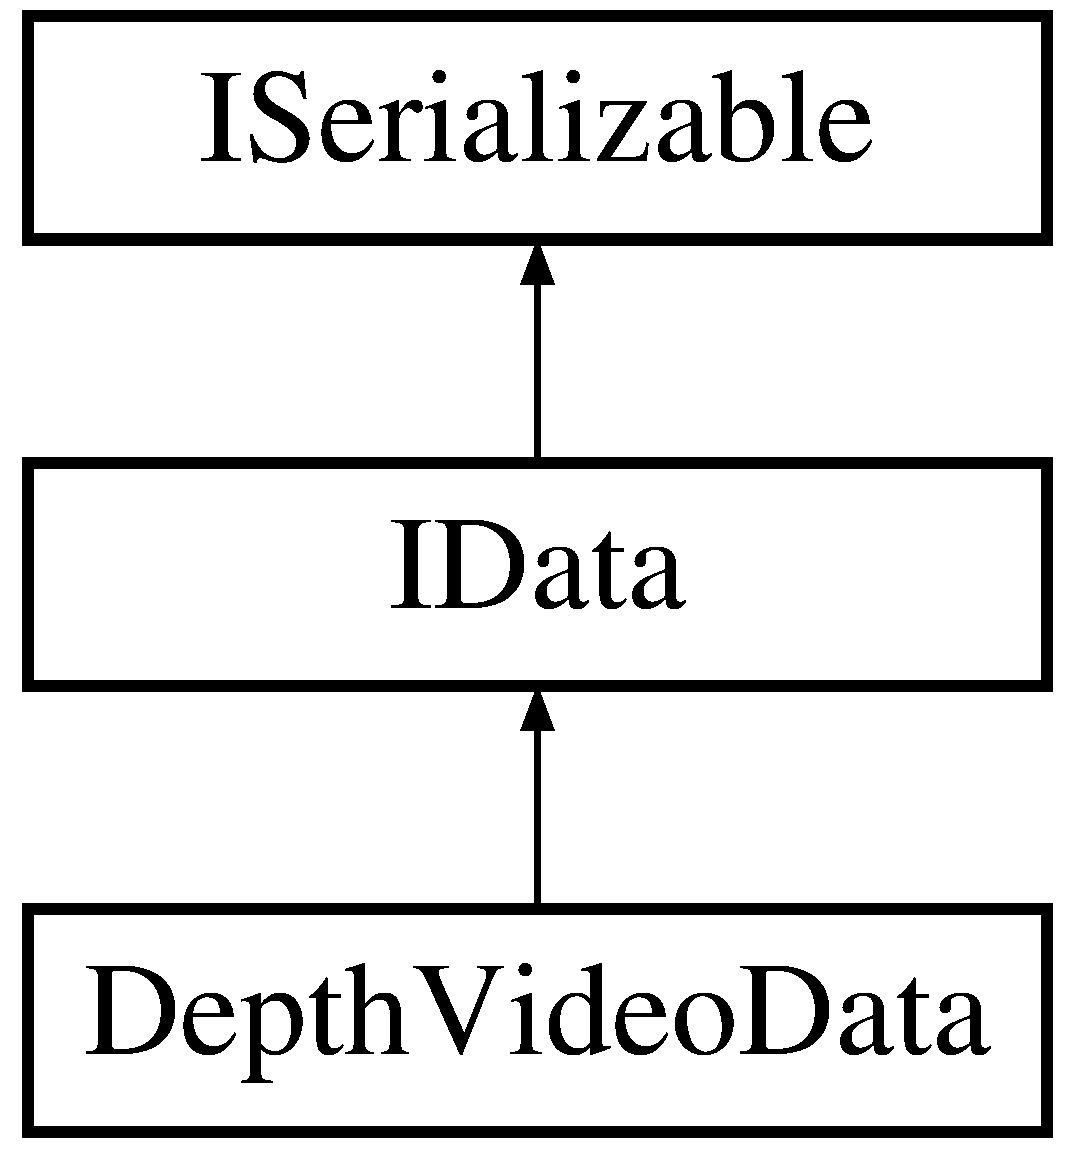
\includegraphics[height=3.000000cm]{class_depth_video_data}
\end{center}
\end{figure}
\subsection*{Public Member Functions}
\begin{DoxyCompactItemize}
\item 
\mbox{\Hypertarget{class_depth_video_data_a6b3312129563abc81bba2a690b11d12e}\label{class_depth_video_data_a6b3312129563abc81bba2a690b11d12e}} 
{\bfseries R\+T\+T\+I\+\_\+\+D\+E\+CL} ()
\item 
\mbox{\Hypertarget{class_depth_video_data_a72644ddffe7de073e34a248c3cbec3ce}\label{class_depth_video_data_a72644ddffe7de073e34a248c3cbec3ce}} 
{\bfseries Depth\+Video\+Data} (std\+::vector$<$ unsigned char $>$ a\+\_\+\+Binary\+Data)
\item 
\mbox{\Hypertarget{class_depth_video_data_a41fd5698a463d0a6efa0039ebbfb05f4}\label{class_depth_video_data_a41fd5698a463d0a6efa0039ebbfb05f4}} 
{\bfseries Depth\+Video\+Data} (const unsigned char $\ast$a\+\_\+p\+Binary\+Data, int a\+\_\+\+Binary\+Length)
\item 
\mbox{\Hypertarget{class_depth_video_data_affa3c056b75c1920183babd1bf9bb63c}\label{class_depth_video_data_affa3c056b75c1920183babd1bf9bb63c}} 
virtual void \hyperlink{class_depth_video_data_affa3c056b75c1920183babd1bf9bb63c}{Serialize} (Json\+::\+Value \&json)
\begin{DoxyCompactList}\small\item\em I\+Serializable interface. \end{DoxyCompactList}\item 
\mbox{\Hypertarget{class_depth_video_data_aacfe6c0c25219273735f0951d299f5d2}\label{class_depth_video_data_aacfe6c0c25219273735f0951d299f5d2}} 
virtual void {\bfseries Deserialize} (const Json\+::\+Value \&json)
\item 
\mbox{\Hypertarget{class_depth_video_data_a0902f7a270581cd84d79866f0273680e}\label{class_depth_video_data_a0902f7a270581cd84d79866f0273680e}} 
virtual bool \hyperlink{class_depth_video_data_a0902f7a270581cd84d79866f0273680e}{To\+Binary} (std\+::string \&a\+\_\+\+Output)
\begin{DoxyCompactList}\small\item\em \hyperlink{class_i_data}{I\+Data} interface. \end{DoxyCompactList}\item 
\mbox{\Hypertarget{class_depth_video_data_ab0f785e8e3a260363e360c1f32297268}\label{class_depth_video_data_ab0f785e8e3a260363e360c1f32297268}} 
virtual bool {\bfseries From\+Binary} (const std\+::string \&a\+\_\+\+Type, const std\+::string \&a\+\_\+\+Input)
\item 
\mbox{\Hypertarget{class_depth_video_data_aa484924fea12da3b835754ea7f21c09a}\label{class_depth_video_data_aa484924fea12da3b835754ea7f21c09a}} 
const std\+::string \& \hyperlink{class_depth_video_data_aa484924fea12da3b835754ea7f21c09a}{Get\+Binary\+Data} () const
\begin{DoxyCompactList}\small\item\em Accessors. \end{DoxyCompactList}\end{DoxyCompactItemize}


The documentation for this class was generated from the following file\+:\begin{DoxyCompactItemize}
\item 
src/sensors/Depth\+Video\+Data.\+h\end{DoxyCompactItemize}

\hypertarget{class_d_f_t}{}\section{D\+FT Class Reference}
\label{class_d_f_t}\index{D\+FT@{D\+FT}}
Inheritance diagram for D\+FT\+:\begin{figure}[H]
\begin{center}
\leavevmode
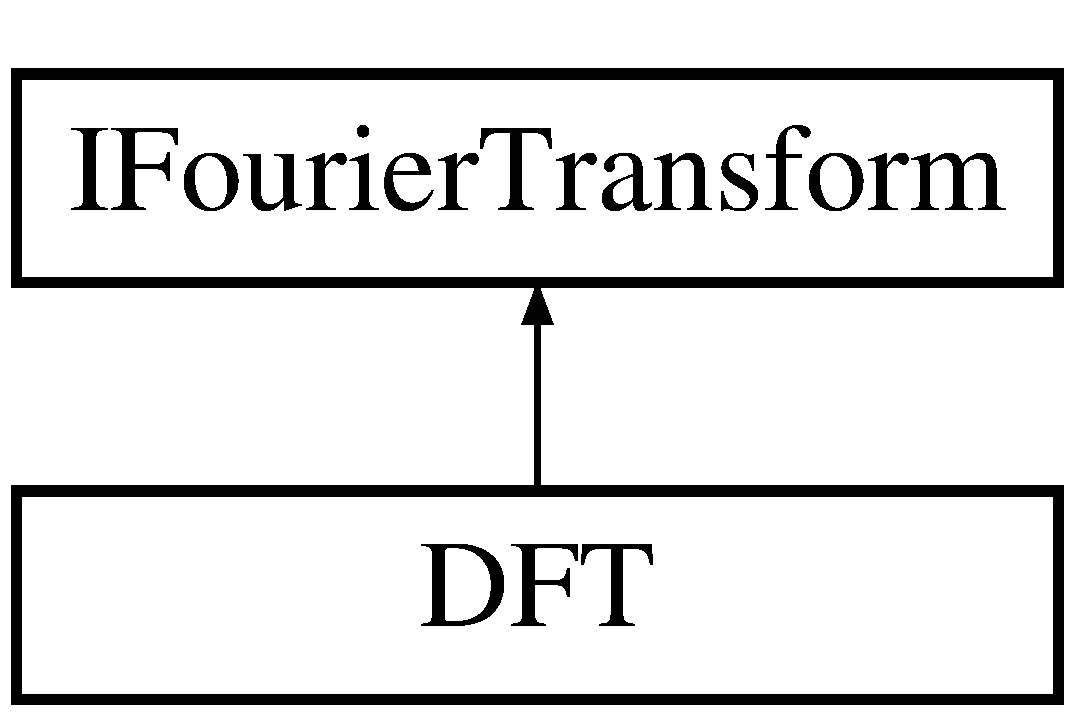
\includegraphics[height=2.000000cm]{class_d_f_t}
\end{center}
\end{figure}
\subsection*{Public Member Functions}
\begin{DoxyCompactItemize}
\item 
void \hyperlink{class_d_f_t_a6d875398a127f4ba5d21cb0ad9ef370b}{Initialize} (int time\+Size, float sample\+Rate)
\item 
\mbox{\Hypertarget{class_d_f_t_ad211ae3ef47bc3a600a6e6a1f4b80645}\label{class_d_f_t_ad211ae3ef47bc3a600a6e6a1f4b80645}} 
virtual void \hyperlink{class_d_f_t_ad211ae3ef47bc3a600a6e6a1f4b80645}{Allocate\+Arrays} ()
\begin{DoxyCompactList}\small\item\em Fourier\+Transform interface. \end{DoxyCompactList}\item 
\mbox{\Hypertarget{class_d_f_t_a309b8cc11df7a9da7ffb639205f4592f}\label{class_d_f_t_a309b8cc11df7a9da7ffb639205f4592f}} 
virtual void {\bfseries Scale\+Band} (int i, float s)
\item 
\mbox{\Hypertarget{class_d_f_t_ae9a74e8d1ec2df33bb82f6b2b5fcb7be}\label{class_d_f_t_ae9a74e8d1ec2df33bb82f6b2b5fcb7be}} 
virtual void {\bfseries Set\+Band} (int i, float a)
\item 
\mbox{\Hypertarget{class_d_f_t_ab4135f3e10bf43ce69ce4a63a82a20b0}\label{class_d_f_t_ab4135f3e10bf43ce69ce4a63a82a20b0}} 
virtual void {\bfseries Forward} (std\+::vector$<$ float $>$ \&a\+\_\+\+Samples, int a\+\_\+n\+Offset=0)
\item 
\mbox{\Hypertarget{class_d_f_t_ab5ba9360f68db15eb4c61eab019df0d0}\label{class_d_f_t_ab5ba9360f68db15eb4c61eab019df0d0}} 
virtual void {\bfseries Inverse} (std\+::vector$<$ float $>$ \&a\+\_\+\+Samples, int a\+\_\+n\+Offset=0)
\end{DoxyCompactItemize}
\subsection*{Additional Inherited Members}


\subsection{Member Function Documentation}
\mbox{\Hypertarget{class_d_f_t_a6d875398a127f4ba5d21cb0ad9ef370b}\label{class_d_f_t_a6d875398a127f4ba5d21cb0ad9ef370b}} 
\index{D\+FT@{D\+FT}!Initialize@{Initialize}}
\index{Initialize@{Initialize}!D\+FT@{D\+FT}}
\subsubsection{\texorpdfstring{Initialize()}{Initialize()}}
{\footnotesize\ttfamily void D\+F\+T\+::\+Initialize (\begin{DoxyParamCaption}\item[{int}]{time\+Size,  }\item[{float}]{sample\+Rate }\end{DoxyParamCaption})\hspace{0.3cm}{\ttfamily [inline]}}

Constructs a \hyperlink{class_d_f_t}{D\+FT} that expects audio buffers of length {\ttfamily time\+Size} that have been recorded with a sample rate of {\ttfamily sample\+Rate}. Will throw an Illegal\+Argument\+Exception if {\ttfamily time\+Size} is not even.


\begin{DoxyParams}{Parameters}
{\em time\+Size} & the length of the audio buffers you plan to analyze \\
\hline
{\em sample\+Rate} & the sample rate of the audio samples you plan to analyze \\
\hline
\end{DoxyParams}


The documentation for this class was generated from the following file\+:\begin{DoxyCompactItemize}
\item 
src/utils/fft/D\+F\+T.\+h\end{DoxyCompactItemize}

\hypertarget{class_dialog_n_l_c_proxy}{}\section{Dialog\+N\+L\+C\+Proxy Class Reference}
\label{class_dialog_n_l_c_proxy}\index{Dialog\+N\+L\+C\+Proxy@{Dialog\+N\+L\+C\+Proxy}}
Inheritance diagram for Dialog\+N\+L\+C\+Proxy\+:\begin{figure}[H]
\begin{center}
\leavevmode
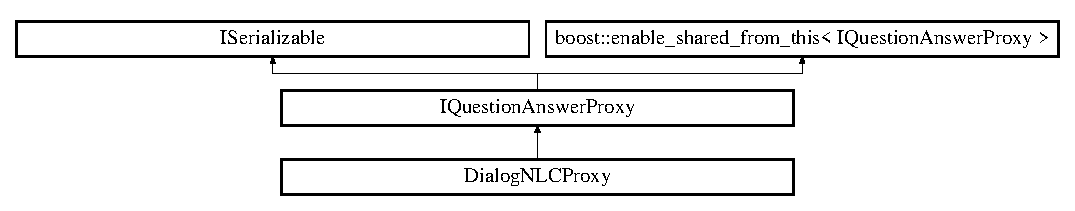
\includegraphics[height=2.393162cm]{class_dialog_n_l_c_proxy}
\end{center}
\end{figure}
\subsection*{Public Member Functions}
\begin{DoxyCompactItemize}
\item 
\mbox{\Hypertarget{class_dialog_n_l_c_proxy_a1b6b689517b0103a5d0b0a3b4b7fafba}\label{class_dialog_n_l_c_proxy_a1b6b689517b0103a5d0b0a3b4b7fafba}} 
{\bfseries R\+T\+T\+I\+\_\+\+D\+E\+CL} ()
\item 
\mbox{\Hypertarget{class_dialog_n_l_c_proxy_abc5a3b5cede5d67fc8f593f32d5a008b}\label{class_dialog_n_l_c_proxy_abc5a3b5cede5d67fc8f593f32d5a008b}} 
virtual void \hyperlink{class_dialog_n_l_c_proxy_abc5a3b5cede5d67fc8f593f32d5a008b}{Start} ()
\begin{DoxyCompactList}\small\item\em I\+Question\+Answer Interface. \end{DoxyCompactList}\item 
\mbox{\Hypertarget{class_dialog_n_l_c_proxy_ae341782818f10ba385d53876294ce4b2}\label{class_dialog_n_l_c_proxy_ae341782818f10ba385d53876294ce4b2}} 
virtual void {\bfseries Stop} ()
\item 
\mbox{\Hypertarget{class_dialog_n_l_c_proxy_a4fbafd1ebce6010f2c1b9e5260dac76e}\label{class_dialog_n_l_c_proxy_a4fbafd1ebce6010f2c1b9e5260dac76e}} 
virtual void {\bfseries Ask\+Question} (\hyperlink{class_question_intent_a250dceb08e1342574a0aca4fe40a7121}{Question\+Intent\+::\+SP} a\+\_\+sp\+Question, Delegate$<$ const Json\+::\+Value \&$>$ a\+\_\+\+Callback)
\item 
\mbox{\Hypertarget{class_dialog_n_l_c_proxy_abf3fd819768c9502ebfa8a995ae14e6b}\label{class_dialog_n_l_c_proxy_abf3fd819768c9502ebfa8a995ae14e6b}} 
virtual void \hyperlink{class_dialog_n_l_c_proxy_abf3fd819768c9502ebfa8a995ae14e6b}{Serialize} (Json\+::\+Value \&json)
\begin{DoxyCompactList}\small\item\em I\+Serializable. \end{DoxyCompactList}\item 
\mbox{\Hypertarget{class_dialog_n_l_c_proxy_a6940d780855d08e154fcc2d3f21504bc}\label{class_dialog_n_l_c_proxy_a6940d780855d08e154fcc2d3f21504bc}} 
virtual void {\bfseries Deserialize} (const Json\+::\+Value \&json)
\item 
\mbox{\Hypertarget{class_dialog_n_l_c_proxy_a1ebe5b56a302b75e03d85355f6904084}\label{class_dialog_n_l_c_proxy_a1ebe5b56a302b75e03d85355f6904084}} 
void \hyperlink{class_dialog_n_l_c_proxy_a1ebe5b56a302b75e03d85355f6904084}{Update} ()
\begin{DoxyCompactList}\small\item\em \hyperlink{class_dialog_n_l_c_proxy}{Dialog\+N\+L\+C\+Proxy} specific. \end{DoxyCompactList}\item 
\mbox{\Hypertarget{class_dialog_n_l_c_proxy_ad77e41ba6d867c4c1dce0129d84c827b}\label{class_dialog_n_l_c_proxy_ad77e41ba6d867c4c1dce0129d84c827b}} 
bool {\bfseries Dialog\+Started} ()
\item 
\mbox{\Hypertarget{class_dialog_n_l_c_proxy_aaaba7d67a342a17d7b751593f07f820e}\label{class_dialog_n_l_c_proxy_aaaba7d67a342a17d7b751593f07f820e}} 
bool {\bfseries Matching\+Dialog\+ID} (const std\+::string \&a\+\_\+\+Dialog\+ID)
\item 
\mbox{\Hypertarget{class_dialog_n_l_c_proxy_a3f5985550af486469d6eb2f6e7c9b7b9}\label{class_dialog_n_l_c_proxy_a3f5985550af486469d6eb2f6e7c9b7b9}} 
void {\bfseries Ask\+Confirm} (const std\+::string \&a\+\_\+\+Confirm, Delegate$<$ const Json\+::\+Value \&$>$ a\+\_\+\+Callback)
\end{DoxyCompactItemize}
\subsection*{Additional Inherited Members}


The documentation for this class was generated from the following files\+:\begin{DoxyCompactItemize}
\item 
src/agent/proxies/Dialog\+N\+L\+C\+Proxy.\+h\item 
src/agent/proxies/Dialog\+N\+L\+C\+Proxy.\+cpp\end{DoxyCompactItemize}

\hypertarget{class_discovery_agent}{}\section{Discovery\+Agent Class Reference}
\label{class_discovery_agent}\index{Discovery\+Agent@{Discovery\+Agent}}
Inheritance diagram for Discovery\+Agent\+:\begin{figure}[H]
\begin{center}
\leavevmode
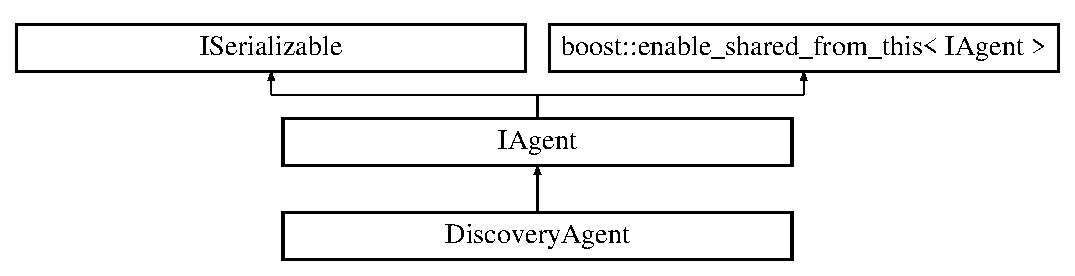
\includegraphics[height=3.000000cm]{class_discovery_agent}
\end{center}
\end{figure}
\subsection*{Classes}
\begin{DoxyCompactItemize}
\item 
struct \hyperlink{struct_discovery_agent_1_1_instance}{Instance}
\begin{DoxyCompactList}\small\item\em Types. \end{DoxyCompactList}\end{DoxyCompactItemize}
\subsection*{Public Types}
\begin{DoxyCompactItemize}
\item 
\mbox{\Hypertarget{class_discovery_agent_afa9e22368a2594a1d131c39047565387}\label{class_discovery_agent_afa9e22368a2594a1d131c39047565387}} 
typedef std\+::vector$<$ Instance\+::\+SP $>$ {\bfseries Instances}
\end{DoxyCompactItemize}
\subsection*{Public Member Functions}
\begin{DoxyCompactItemize}
\item 
\mbox{\Hypertarget{class_discovery_agent_a2588146e902e5d257ca271b069375f6b}\label{class_discovery_agent_a2588146e902e5d257ca271b069375f6b}} 
{\bfseries R\+T\+T\+I\+\_\+\+D\+E\+CL} ()
\item 
\mbox{\Hypertarget{class_discovery_agent_a67363475dc274fd8b759f9a263077b24}\label{class_discovery_agent_a67363475dc274fd8b759f9a263077b24}} 
\hyperlink{class_discovery_agent_a67363475dc274fd8b759f9a263077b24}{Discovery\+Agent} ()
\begin{DoxyCompactList}\small\item\em Construction. \end{DoxyCompactList}\item 
\mbox{\Hypertarget{class_discovery_agent_a50f62278b7937a8d6570def984a45f3e}\label{class_discovery_agent_a50f62278b7937a8d6570def984a45f3e}} 
void \hyperlink{class_discovery_agent_a50f62278b7937a8d6570def984a45f3e}{Serialize} (Json\+::\+Value \&json)
\begin{DoxyCompactList}\small\item\em I\+Serializable interface. \end{DoxyCompactList}\item 
\mbox{\Hypertarget{class_discovery_agent_a274bf13dc2c1710c2b5bad7adf761ab0}\label{class_discovery_agent_a274bf13dc2c1710c2b5bad7adf761ab0}} 
void {\bfseries Deserialize} (const Json\+::\+Value \&json)
\item 
\mbox{\Hypertarget{class_discovery_agent_a113c33de751fd40a24e416c0eb7e5a3e}\label{class_discovery_agent_a113c33de751fd40a24e416c0eb7e5a3e}} 
virtual bool \hyperlink{class_discovery_agent_a113c33de751fd40a24e416c0eb7e5a3e}{On\+Start} ()
\begin{DoxyCompactList}\small\item\em \hyperlink{class_i_agent}{I\+Agent} interface. \end{DoxyCompactList}\item 
\mbox{\Hypertarget{class_discovery_agent_add71af911778441d2c032d4ad8ad6a86}\label{class_discovery_agent_add71af911778441d2c032d4ad8ad6a86}} 
virtual bool {\bfseries On\+Stop} ()
\item 
\mbox{\Hypertarget{class_discovery_agent_a677f2a9afb0f85709fdb83b9c57e3800}\label{class_discovery_agent_a677f2a9afb0f85709fdb83b9c57e3800}} 
const Instances \& \hyperlink{class_discovery_agent_a677f2a9afb0f85709fdb83b9c57e3800}{Get\+Discovered} () const
\begin{DoxyCompactList}\small\item\em Accessors. \end{DoxyCompactList}\end{DoxyCompactItemize}
\subsection*{Additional Inherited Members}


The documentation for this class was generated from the following files\+:\begin{DoxyCompactItemize}
\item 
src/agent/Discovery\+Agent.\+h\item 
src/agent/Discovery\+Agent.\+cpp\end{DoxyCompactItemize}

\hypertarget{class_disk_audio_sensor}{}\section{Disk\+Audio\+Sensor Class Reference}
\label{class_disk_audio_sensor}\index{Disk\+Audio\+Sensor@{Disk\+Audio\+Sensor}}
Inheritance diagram for Disk\+Audio\+Sensor\+:\begin{figure}[H]
\begin{center}
\leavevmode
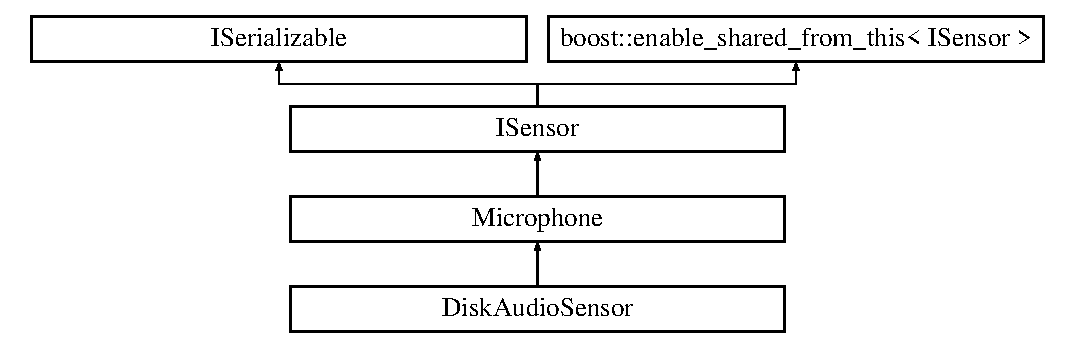
\includegraphics[height=4.000000cm]{class_disk_audio_sensor}
\end{center}
\end{figure}
\subsection*{Public Types}
\begin{DoxyCompactItemize}
\item 
\mbox{\Hypertarget{class_disk_audio_sensor_ace31aa7c9c8645b0355f4ddcb61c6611}\label{class_disk_audio_sensor_ace31aa7c9c8645b0355f4ddcb61c6611}} 
typedef boost\+::shared\+\_\+ptr$<$ \hyperlink{class_disk_audio_sensor}{Disk\+Audio\+Sensor} $>$ \hyperlink{class_disk_audio_sensor_ace31aa7c9c8645b0355f4ddcb61c6611}{SP}
\begin{DoxyCompactList}\small\item\em Types. \end{DoxyCompactList}\item 
\mbox{\Hypertarget{class_disk_audio_sensor_a6207eaecaac1d6b390f715d07d9b08a2}\label{class_disk_audio_sensor_a6207eaecaac1d6b390f715d07d9b08a2}} 
typedef boost\+::weak\+\_\+ptr$<$ \hyperlink{class_disk_audio_sensor}{Disk\+Audio\+Sensor} $>$ {\bfseries WP}
\end{DoxyCompactItemize}
\subsection*{Public Member Functions}
\begin{DoxyCompactItemize}
\item 
\mbox{\Hypertarget{class_disk_audio_sensor_ab7a536d98f84a415e1e594ee6b67d285}\label{class_disk_audio_sensor_ab7a536d98f84a415e1e594ee6b67d285}} 
{\bfseries R\+T\+T\+I\+\_\+\+D\+E\+CL} ()
\item 
\mbox{\Hypertarget{class_disk_audio_sensor_af2c053fa2821b9e4f72ffefdfc831229}\label{class_disk_audio_sensor_af2c053fa2821b9e4f72ffefdfc831229}} 
\hyperlink{class_disk_audio_sensor_af2c053fa2821b9e4f72ffefdfc831229}{Disk\+Audio\+Sensor} ()
\begin{DoxyCompactList}\small\item\em Construction. \end{DoxyCompactList}\item 
\mbox{\Hypertarget{class_disk_audio_sensor_acfa38d87a557de544ec7fb16d1a7f464}\label{class_disk_audio_sensor_acfa38d87a557de544ec7fb16d1a7f464}} 
void \hyperlink{class_disk_audio_sensor_acfa38d87a557de544ec7fb16d1a7f464}{Serialize} (Json\+::\+Value \&json)
\begin{DoxyCompactList}\small\item\em I\+Serializable interface. \end{DoxyCompactList}\item 
\mbox{\Hypertarget{class_disk_audio_sensor_ad4a871a18e5c375ee60e7cf4a13ba59a}\label{class_disk_audio_sensor_ad4a871a18e5c375ee60e7cf4a13ba59a}} 
void {\bfseries Deserialize} (const Json\+::\+Value \&json)
\item 
\mbox{\Hypertarget{class_disk_audio_sensor_ac0deead63e4f35c90cf32a4046084e92}\label{class_disk_audio_sensor_ac0deead63e4f35c90cf32a4046084e92}} 
virtual const char $\ast$ \hyperlink{class_disk_audio_sensor_ac0deead63e4f35c90cf32a4046084e92}{Get\+Sensor\+Name} ()
\begin{DoxyCompactList}\small\item\em \hyperlink{class_i_sensor}{I\+Sensor} interface. \end{DoxyCompactList}\item 
\mbox{\Hypertarget{class_disk_audio_sensor_ae39fded0d11e45d915ac7141ebf70c53}\label{class_disk_audio_sensor_ae39fded0d11e45d915ac7141ebf70c53}} 
virtual const char $\ast$ {\bfseries Get\+Data\+Type} ()
\item 
\mbox{\Hypertarget{class_disk_audio_sensor_a77d25c71d6978e80f2202f417fbb4192}\label{class_disk_audio_sensor_a77d25c71d6978e80f2202f417fbb4192}} 
const std\+::string \& {\bfseries Get\+Recordings\+Path} () const
\item 
\mbox{\Hypertarget{class_disk_audio_sensor_a2dd5b3d98892282b5764f7354d30cda1}\label{class_disk_audio_sensor_a2dd5b3d98892282b5764f7354d30cda1}} 
bool {\bfseries Get\+Capture\+Stopped} ()
\item 
\mbox{\Hypertarget{class_disk_audio_sensor_af8d84b4e6eb932ecd342a824e8c9d79e}\label{class_disk_audio_sensor_af8d84b4e6eb932ecd342a824e8c9d79e}} 
virtual bool \hyperlink{class_disk_audio_sensor_af8d84b4e6eb932ecd342a824e8c9d79e}{On\+Start} ()
\begin{DoxyCompactList}\small\item\em This is invoked when the first subscriber subscribes to this sensor. \end{DoxyCompactList}\item 
\mbox{\Hypertarget{class_disk_audio_sensor_ae0a2904cd8b1115d25e3fbfec733ed15}\label{class_disk_audio_sensor_ae0a2904cd8b1115d25e3fbfec733ed15}} 
virtual bool \hyperlink{class_disk_audio_sensor_ae0a2904cd8b1115d25e3fbfec733ed15}{On\+Stop} ()
\begin{DoxyCompactList}\small\item\em This is invoked when the last subscriber un-\/subscribes. \end{DoxyCompactList}\item 
\mbox{\Hypertarget{class_disk_audio_sensor_ab77e804b5c6afb2333466dcc77a55b31}\label{class_disk_audio_sensor_ab77e804b5c6afb2333466dcc77a55b31}} 
virtual void \hyperlink{class_disk_audio_sensor_ab77e804b5c6afb2333466dcc77a55b31}{On\+Pause} ()
\begin{DoxyCompactList}\small\item\em This is invoked to pause this sensor. \end{DoxyCompactList}\item 
\mbox{\Hypertarget{class_disk_audio_sensor_a6de062e47ee854ab1f041325b3963426}\label{class_disk_audio_sensor_a6de062e47ee854ab1f041325b3963426}} 
virtual void \hyperlink{class_disk_audio_sensor_a6de062e47ee854ab1f041325b3963426}{On\+Resume} ()
\begin{DoxyCompactList}\small\item\em This is invoked to restart this sensor. \end{DoxyCompactList}\end{DoxyCompactItemize}
\subsection*{Additional Inherited Members}


The documentation for this class was generated from the following files\+:\begin{DoxyCompactItemize}
\item 
src/sensors/Disk\+Audio\+Sensor.\+h\item 
src/sensors/Disk\+Audio\+Sensor.\+cpp\end{DoxyCompactItemize}

\hypertarget{class_display}{}\section{Display Class Reference}
\label{class_display}\index{Display@{Display}}


This object is placed on the blackboard when we need self to say anything.  




{\ttfamily \#include $<$Display.\+h$>$}

Inheritance diagram for Display\+:\begin{figure}[H]
\begin{center}
\leavevmode
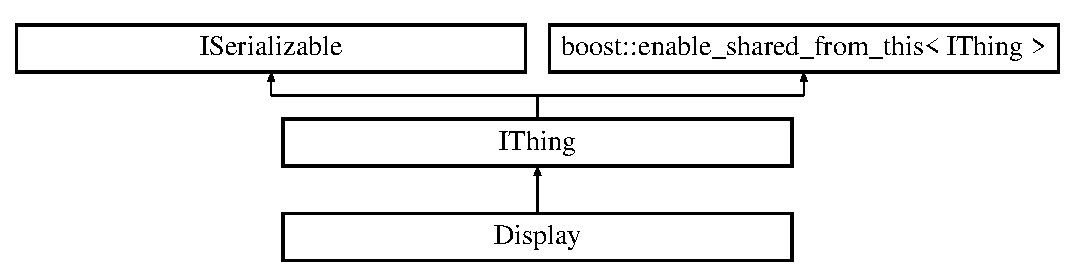
\includegraphics[height=3.000000cm]{class_display}
\end{center}
\end{figure}
\subsection*{Public Types}
\begin{DoxyCompactItemize}
\item 
\mbox{\Hypertarget{class_display_a6c34a315a515aeeb75a369d4aba4d7b3}\label{class_display_a6c34a315a515aeeb75a369d4aba4d7b3}} 
typedef boost\+::shared\+\_\+ptr$<$ \hyperlink{class_display}{Display} $>$ \hyperlink{class_display_a6c34a315a515aeeb75a369d4aba4d7b3}{SP}
\begin{DoxyCompactList}\small\item\em Types. \end{DoxyCompactList}\item 
\mbox{\Hypertarget{class_display_a47d87d5f6a553e18403de6549580dbaf}\label{class_display_a47d87d5f6a553e18403de6549580dbaf}} 
typedef boost\+::weak\+\_\+ptr$<$ \hyperlink{class_display}{Display} $>$ {\bfseries WP}
\end{DoxyCompactItemize}
\subsection*{Public Member Functions}
\begin{DoxyCompactItemize}
\item 
\mbox{\Hypertarget{class_display_ac381760387be9c662b29efa120be2232}\label{class_display_ac381760387be9c662b29efa120be2232}} 
{\bfseries R\+T\+T\+I\+\_\+\+D\+E\+CL} ()
\item 
\mbox{\Hypertarget{class_display_abe3f2917dc53984aed26ce3fde15d82f}\label{class_display_abe3f2917dc53984aed26ce3fde15d82f}} 
virtual void \hyperlink{class_display_abe3f2917dc53984aed26ce3fde15d82f}{Serialize} (Json\+::\+Value \&json)
\begin{DoxyCompactList}\small\item\em I\+Serializable interface. \end{DoxyCompactList}\item 
\mbox{\Hypertarget{class_display_a5f74bc892861390b9453e9fdd49920ab}\label{class_display_a5f74bc892861390b9453e9fdd49920ab}} 
virtual void {\bfseries Deserialize} (const Json\+::\+Value \&json)
\item 
\mbox{\Hypertarget{class_display_ae972fffea6f7ca1d627ef48c3d841bb3}\label{class_display_ae972fffea6f7ca1d627ef48c3d841bb3}} 
\hyperlink{class_display_ae972fffea6f7ca1d627ef48c3d841bb3}{Display} ()
\begin{DoxyCompactList}\small\item\em Construction. \end{DoxyCompactList}\item 
\mbox{\Hypertarget{class_display_aa39c7a9b32afa85e78a302ef37d4b0da}\label{class_display_aa39c7a9b32afa85e78a302ef37d4b0da}} 
{\bfseries Display} (const std\+::string \&a\+\_\+\+Display\+Type, const std\+::string \&a\+\_\+\+Data)
\item 
\mbox{\Hypertarget{class_display_ad74675a76e48a7641883ab5174e4f0ba}\label{class_display_ad74675a76e48a7641883ab5174e4f0ba}} 
const std\+::string \& \hyperlink{class_display_ad74675a76e48a7641883ab5174e4f0ba}{Get\+Display} () const
\begin{DoxyCompactList}\small\item\em Accessors. \end{DoxyCompactList}\item 
\mbox{\Hypertarget{class_display_a123014b3e7fedeb5bba3dc9cc9ebee75}\label{class_display_a123014b3e7fedeb5bba3dc9cc9ebee75}} 
void {\bfseries Set\+Display} (const std\+::string \&a\+\_\+\+Display\+Type)
\item 
\mbox{\Hypertarget{class_display_af8d0f143fba382ceefeaa4413cd32c95}\label{class_display_af8d0f143fba382ceefeaa4413cd32c95}} 
const std\+::string \& {\bfseries Get\+Data} () const
\item 
\mbox{\Hypertarget{class_display_ad664fc5ec24557a46097e1e893499985}\label{class_display_ad664fc5ec24557a46097e1e893499985}} 
void {\bfseries Set\+Data} (const std\+::string \&a\+\_\+\+Data)
\end{DoxyCompactItemize}
\subsection*{Additional Inherited Members}


\subsection{Detailed Description}
This object is placed on the blackboard when we need self to say anything. 

The documentation for this class was generated from the following files\+:\begin{DoxyCompactItemize}
\item 
src/blackboard/Display.\+h\item 
src/blackboard/Display.\+cpp\end{DoxyCompactItemize}

\hypertarget{class_display_agent}{}\section{Display\+Agent Class Reference}
\label{class_display_agent}\index{Display\+Agent@{Display\+Agent}}
Inheritance diagram for Display\+Agent\+:\begin{figure}[H]
\begin{center}
\leavevmode
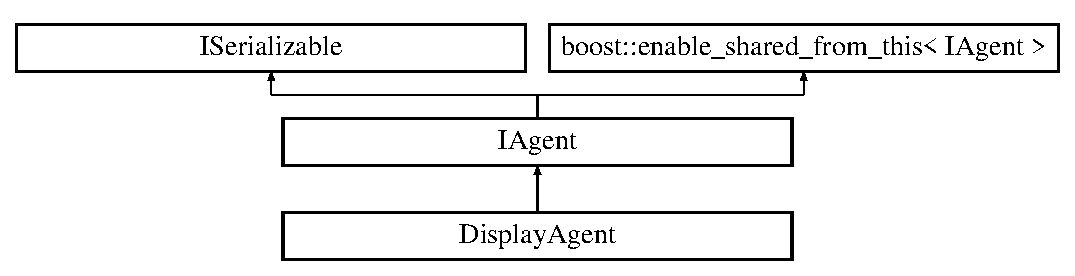
\includegraphics[height=3.000000cm]{class_display_agent}
\end{center}
\end{figure}
\subsection*{Public Member Functions}
\begin{DoxyCompactItemize}
\item 
\mbox{\Hypertarget{class_display_agent_a16531a8ef93495143494ca0ae6c7e689}\label{class_display_agent_a16531a8ef93495143494ca0ae6c7e689}} 
{\bfseries R\+T\+T\+I\+\_\+\+D\+E\+CL} ()
\item 
\mbox{\Hypertarget{class_display_agent_a03531a5286a1f5c9436903d0fdbae013}\label{class_display_agent_a03531a5286a1f5c9436903d0fdbae013}} 
void \hyperlink{class_display_agent_a03531a5286a1f5c9436903d0fdbae013}{Serialize} (Json\+::\+Value \&json)
\begin{DoxyCompactList}\small\item\em I\+Serializable interface. \end{DoxyCompactList}\item 
\mbox{\Hypertarget{class_display_agent_aa0072c3096aa9982c75a79de09bbb1eb}\label{class_display_agent_aa0072c3096aa9982c75a79de09bbb1eb}} 
void {\bfseries Deserialize} (const Json\+::\+Value \&json)
\item 
\mbox{\Hypertarget{class_display_agent_a0250faa8d9b893fca60982a480ab9ac0}\label{class_display_agent_a0250faa8d9b893fca60982a480ab9ac0}} 
virtual bool \hyperlink{class_display_agent_a0250faa8d9b893fca60982a480ab9ac0}{On\+Start} ()
\begin{DoxyCompactList}\small\item\em \hyperlink{class_i_agent}{I\+Agent} interface. \end{DoxyCompactList}\item 
\mbox{\Hypertarget{class_display_agent_a86e4ad8c90b707f3f8206b15b3cdf609}\label{class_display_agent_a86e4ad8c90b707f3f8206b15b3cdf609}} 
virtual bool {\bfseries On\+Stop} ()
\end{DoxyCompactItemize}
\subsection*{Additional Inherited Members}


The documentation for this class was generated from the following files\+:\begin{DoxyCompactItemize}
\item 
src/agent/Display\+Agent.\+h\item 
src/agent/Display\+Agent.\+cpp\end{DoxyCompactItemize}

\hypertarget{class_display_gesture}{}\section{Display\+Gesture Class Reference}
\label{class_display_gesture}\index{Display\+Gesture@{Display\+Gesture}}


This gesture can be used to display a visualization on a screen.  




{\ttfamily \#include $<$Display\+Gesture.\+h$>$}

Inheritance diagram for Display\+Gesture\+:\begin{figure}[H]
\begin{center}
\leavevmode
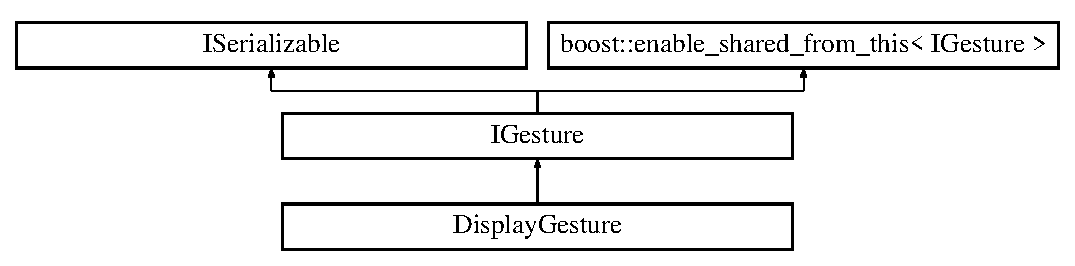
\includegraphics[height=3.000000cm]{class_display_gesture}
\end{center}
\end{figure}
\subsection*{Public Member Functions}
\begin{DoxyCompactItemize}
\item 
\mbox{\Hypertarget{class_display_gesture_a4ee96e56a95a5898cb663fcd8dd35373}\label{class_display_gesture_a4ee96e56a95a5898cb663fcd8dd35373}} 
{\bfseries R\+T\+T\+I\+\_\+\+D\+E\+CL} ()
\item 
\mbox{\Hypertarget{class_display_gesture_a26b9a348bba896bfda9c3e3598c85fba}\label{class_display_gesture_a26b9a348bba896bfda9c3e3598c85fba}} 
\hyperlink{class_display_gesture_a26b9a348bba896bfda9c3e3598c85fba}{Display\+Gesture} ()
\begin{DoxyCompactList}\small\item\em Construction. \end{DoxyCompactList}\item 
\mbox{\Hypertarget{class_display_gesture_a9276a10263e9c9b15efd2d9883f03e66}\label{class_display_gesture_a9276a10263e9c9b15efd2d9883f03e66}} 
virtual void \hyperlink{class_display_gesture_a9276a10263e9c9b15efd2d9883f03e66}{Serialize} (Json\+::\+Value \&json)
\begin{DoxyCompactList}\small\item\em I\+Serializable interface. \end{DoxyCompactList}\item 
\mbox{\Hypertarget{class_display_gesture_a514f7d39f6e12ad451ad97a6e6a83c3e}\label{class_display_gesture_a514f7d39f6e12ad451ad97a6e6a83c3e}} 
virtual void {\bfseries Deserialize} (const Json\+::\+Value \&json)
\item 
\mbox{\Hypertarget{class_display_gesture_ad624cc5eb904d63176eb594fed336ade}\label{class_display_gesture_ad624cc5eb904d63176eb594fed336ade}} 
virtual bool \hyperlink{class_display_gesture_ad624cc5eb904d63176eb594fed336ade}{Can\+Execute} (const \hyperlink{class_params_map}{Params\+Map} \&a\+\_\+\+Params)
\begin{DoxyCompactList}\small\item\em \hyperlink{class_i_gesture}{I\+Gesture} interface. \end{DoxyCompactList}\item 
virtual bool \hyperlink{class_display_gesture_a85bd298434073aa8d384ccbf520ef221}{Execute} (Gesture\+Delegate a\+\_\+\+Callback, const \hyperlink{class_params_map}{Params\+Map} \&a\+\_\+\+Params)
\item 
\mbox{\Hypertarget{class_display_gesture_a46ea9bd9b94cf7a4bd828c5eaa7c87ce}\label{class_display_gesture_a46ea9bd9b94cf7a4bd828c5eaa7c87ce}} 
virtual bool \hyperlink{class_display_gesture_a46ea9bd9b94cf7a4bd828c5eaa7c87ce}{Abort} ()
\begin{DoxyCompactList}\small\item\em Abort this gesture, if true is returned then abort succeeded and callback will N\+OT be invoked. \end{DoxyCompactList}\end{DoxyCompactItemize}
\subsection*{Additional Inherited Members}


\subsection{Detailed Description}
This gesture can be used to display a visualization on a screen. 

\subsection{Member Function Documentation}
\mbox{\Hypertarget{class_display_gesture_a85bd298434073aa8d384ccbf520ef221}\label{class_display_gesture_a85bd298434073aa8d384ccbf520ef221}} 
\index{Display\+Gesture@{Display\+Gesture}!Execute@{Execute}}
\index{Execute@{Execute}!Display\+Gesture@{Display\+Gesture}}
\subsubsection{\texorpdfstring{Execute()}{Execute()}}
{\footnotesize\ttfamily bool Display\+Gesture\+::\+Execute (\begin{DoxyParamCaption}\item[{Gesture\+Delegate}]{a\+\_\+\+Callback,  }\item[{const \hyperlink{class_params_map}{Params\+Map} \&}]{a\+\_\+\+Params }\end{DoxyParamCaption})\hspace{0.3cm}{\ttfamily [virtual]}}

This function will be called by a Skill object, this object should invoke the provided callback when this gesture is done. 

Reimplemented from \hyperlink{class_i_gesture_aa48e38eda852843cab78c22dabfe7371}{I\+Gesture}.



The documentation for this class was generated from the following files\+:\begin{DoxyCompactItemize}
\item 
src/gestures/Display\+Gesture.\+h\item 
src/gestures/Display\+Gesture.\+cpp\end{DoxyCompactItemize}

\hypertarget{class_duplicate_filter}{}\section{Duplicate\+Filter Class Reference}
\label{class_duplicate_filter}\index{Duplicate\+Filter@{Duplicate\+Filter}}


{\ttfamily \#include $<$Duplicate\+Filter.\+h$>$}

Inheritance diagram for Duplicate\+Filter\+:\begin{figure}[H]
\begin{center}
\leavevmode
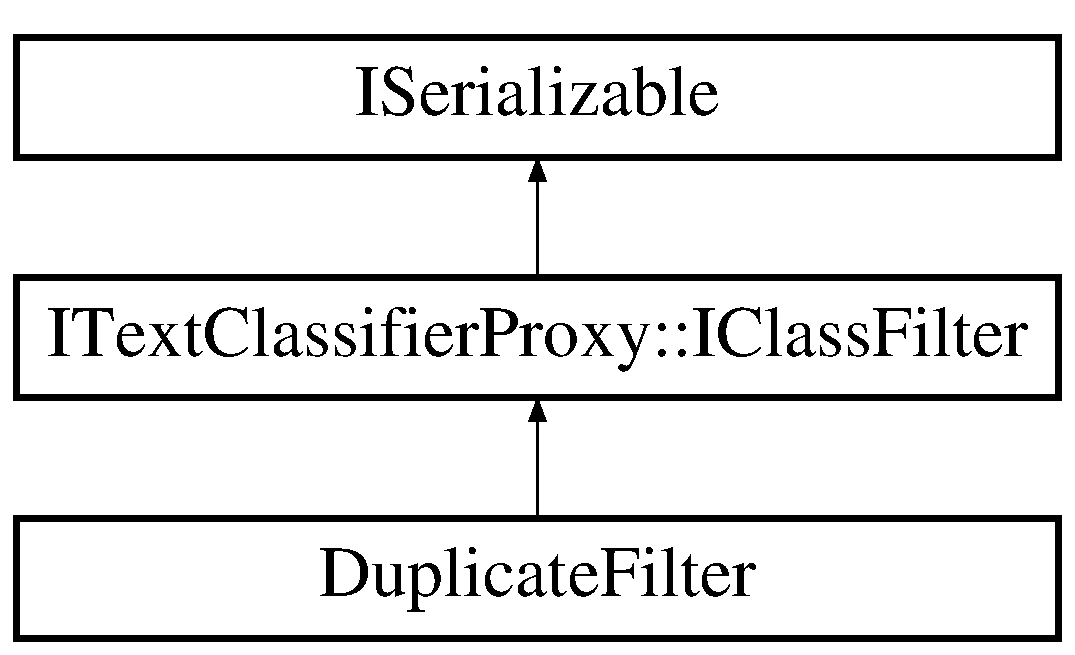
\includegraphics[height=3.000000cm]{class_duplicate_filter}
\end{center}
\end{figure}
\subsection*{Public Member Functions}
\begin{DoxyCompactItemize}
\item 
\mbox{\Hypertarget{class_duplicate_filter_a64917174d78b20ea83040237069f334b}\label{class_duplicate_filter_a64917174d78b20ea83040237069f334b}} 
{\bfseries R\+T\+T\+I\+\_\+\+D\+E\+CL} ()
\item 
\mbox{\Hypertarget{class_duplicate_filter_af83da16afc47b3e76585cafa2b79fe3b}\label{class_duplicate_filter_af83da16afc47b3e76585cafa2b79fe3b}} 
virtual void \hyperlink{class_duplicate_filter_af83da16afc47b3e76585cafa2b79fe3b}{Serialize} (Json\+::\+Value \&json)
\begin{DoxyCompactList}\small\item\em I\+Serialiable interface. \end{DoxyCompactList}\item 
\mbox{\Hypertarget{class_duplicate_filter_a88fc1ec78931b4c6545e76c8e9ea9843}\label{class_duplicate_filter_a88fc1ec78931b4c6545e76c8e9ea9843}} 
virtual void {\bfseries Deserialize} (const Json\+::\+Value \&json)
\item 
\mbox{\Hypertarget{class_duplicate_filter_a7acbdcc9396eca917a2567d986175ea8}\label{class_duplicate_filter_a7acbdcc9396eca917a2567d986175ea8}} 
virtual bool \hyperlink{class_duplicate_filter_a7acbdcc9396eca917a2567d986175ea8}{Apply\+Filter} (Json\+::\+Value \&a\+\_\+\+Intent)
\begin{DoxyCompactList}\small\item\em I\+Class\+Filter interface. \end{DoxyCompactList}\end{DoxyCompactItemize}
\subsection*{Additional Inherited Members}


\subsection{Detailed Description}
This filter looks for the same intent within a time window and will ignore those intents. 

The documentation for this class was generated from the following files\+:\begin{DoxyCompactItemize}
\item 
src/classifiers/filters/Duplicate\+Filter.\+h\item 
src/classifiers/filters/Duplicate\+Filter.\+cpp\end{DoxyCompactItemize}

\hypertarget{class_e_beat_detect}{}\section{E\+Beat\+Detect Class Reference}
\label{class_e_beat_detect}\index{E\+Beat\+Detect@{E\+Beat\+Detect}}
Inheritance diagram for E\+Beat\+Detect\+:\begin{figure}[H]
\begin{center}
\leavevmode
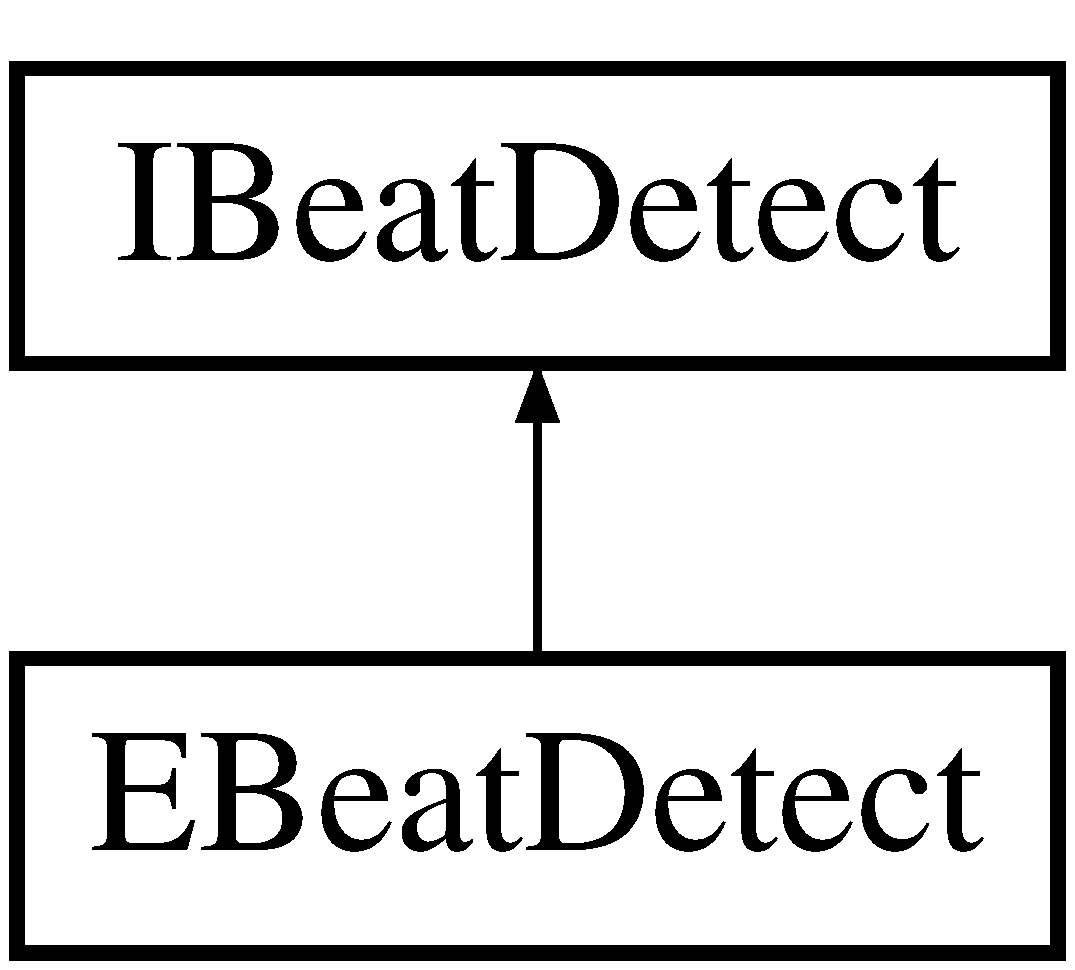
\includegraphics[height=2.000000cm]{class_e_beat_detect}
\end{center}
\end{figure}
\subsection*{Public Member Functions}
\begin{DoxyCompactItemize}
\item 
\mbox{\Hypertarget{class_e_beat_detect_a1e735285d9d7b623c81c23edc72897ca}\label{class_e_beat_detect_a1e735285d9d7b623c81c23edc72897ca}} 
virtual void \hyperlink{class_e_beat_detect_a1e735285d9d7b623c81c23edc72897ca}{Initialize} (int time\+Size, float sample\+Rate)
\begin{DoxyCompactList}\small\item\em Initialize this beat detector. \end{DoxyCompactList}\item 
\mbox{\Hypertarget{class_e_beat_detect_abc1a0d7e9168a2fd76333d2ab61cfced}\label{class_e_beat_detect_abc1a0d7e9168a2fd76333d2ab61cfced}} 
virtual void \hyperlink{class_e_beat_detect_abc1a0d7e9168a2fd76333d2ab61cfced}{Reset} ()
\begin{DoxyCompactList}\small\item\em Release this beat detector. \end{DoxyCompactList}\item 
\mbox{\Hypertarget{class_e_beat_detect_aeb554bcf0fa1974f0fe3f8ad5b403712}\label{class_e_beat_detect_aeb554bcf0fa1974f0fe3f8ad5b403712}} 
virtual bool \hyperlink{class_e_beat_detect_aeb554bcf0fa1974f0fe3f8ad5b403712}{Detect} (std\+::vector$<$ float $>$ \&a\+\_\+\+Samples, size\+\_\+t a\+\_\+n\+Offset)
\begin{DoxyCompactList}\small\item\em Returns true if a onset is detected in this block of audio data. \end{DoxyCompactList}\end{DoxyCompactItemize}
\subsection*{Additional Inherited Members}


The documentation for this class was generated from the following file\+:\begin{DoxyCompactItemize}
\item 
src/utils/fft/E\+Beat\+Detect.\+h\end{DoxyCompactItemize}

\hypertarget{class_graph_self_1_1_edge}{}\section{Graph\+Self\+:\+:Edge Class Reference}
\label{class_graph_self_1_1_edge}\index{Graph\+Self\+::\+Edge@{Graph\+Self\+::\+Edge}}
Inheritance diagram for Graph\+Self\+:\+:Edge\+:\begin{figure}[H]
\begin{center}
\leavevmode
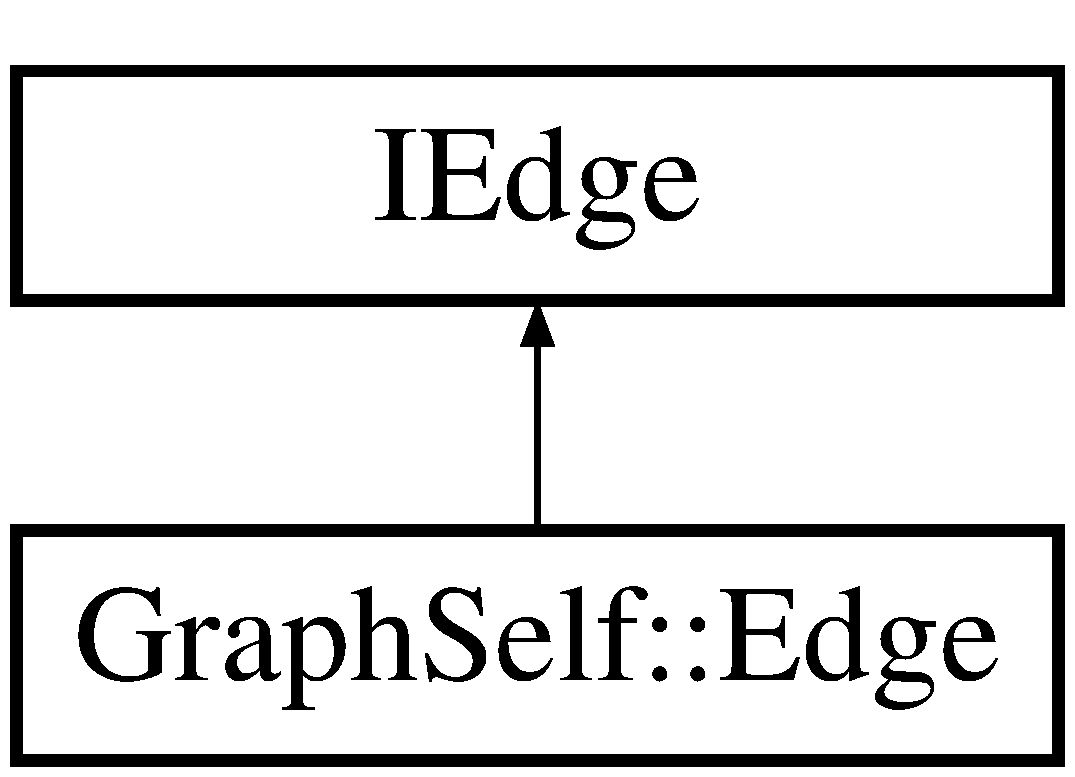
\includegraphics[height=2.000000cm]{class_graph_self_1_1_edge}
\end{center}
\end{figure}
\subsection*{Public Types}
\begin{DoxyCompactItemize}
\item 
\mbox{\Hypertarget{class_graph_self_1_1_edge_a3d61c5aa0974830bf1ad49d7a6ca8066}\label{class_graph_self_1_1_edge_a3d61c5aa0974830bf1ad49d7a6ca8066}} 
typedef boost\+::shared\+\_\+ptr$<$ \hyperlink{class_graph_self_1_1_edge}{Edge} $>$ {\bfseries SP}
\item 
\mbox{\Hypertarget{class_graph_self_1_1_edge_a82161fe91f11aa2780e54fd3807d1dd8}\label{class_graph_self_1_1_edge_a82161fe91f11aa2780e54fd3807d1dd8}} 
typedef boost\+::weak\+\_\+ptr$<$ \hyperlink{class_graph_self_1_1_edge}{Edge} $>$ {\bfseries WP}
\end{DoxyCompactItemize}
\subsection*{Public Member Functions}
\begin{DoxyCompactItemize}
\item 
\mbox{\Hypertarget{class_graph_self_1_1_edge_a83a6b6b4edcc15b745424b4170f68a3b}\label{class_graph_self_1_1_edge_a83a6b6b4edcc15b745424b4170f68a3b}} 
{\bfseries R\+T\+T\+I\+\_\+\+D\+E\+CL} ()
\item 
\mbox{\Hypertarget{class_graph_self_1_1_edge_a21c5a0150dd98700610df657b94bf763}\label{class_graph_self_1_1_edge_a21c5a0150dd98700610df657b94bf763}} 
virtual void \hyperlink{class_graph_self_1_1_edge_a21c5a0150dd98700610df657b94bf763}{Serialize} (Json\+::\+Value \&json)
\begin{DoxyCompactList}\small\item\em I\+Serializable interface. \end{DoxyCompactList}\item 
\mbox{\Hypertarget{class_graph_self_1_1_edge_a33c36713307d7e2419e163b43039e531}\label{class_graph_self_1_1_edge_a33c36713307d7e2419e163b43039e531}} 
virtual void {\bfseries Deserialize} (const Json\+::\+Value \&json)
\end{DoxyCompactItemize}


The documentation for this class was generated from the following files\+:\begin{DoxyCompactItemize}
\item 
src/models/Graph\+Self.\+h\item 
src/models/Graph\+Self.\+cpp\end{DoxyCompactItemize}

\hypertarget{class_email_gesture}{}\section{Email\+Gesture Class Reference}
\label{class_email_gesture}\index{Email\+Gesture@{Email\+Gesture}}


This gesture can use the S\+MS service to send a text message.  




{\ttfamily \#include $<$Email\+Gesture.\+h$>$}

Inheritance diagram for Email\+Gesture\+:\begin{figure}[H]
\begin{center}
\leavevmode
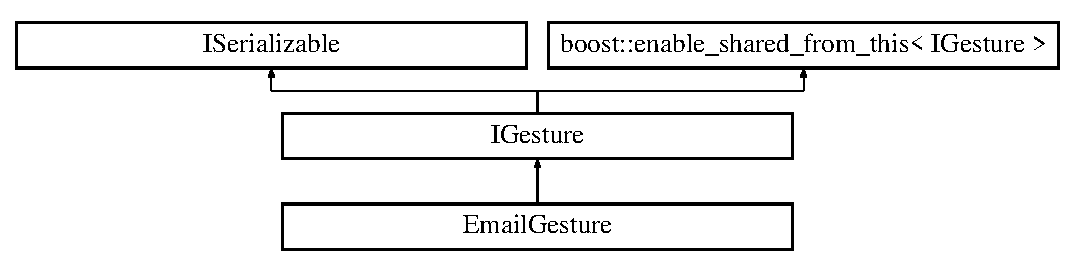
\includegraphics[height=3.000000cm]{class_email_gesture}
\end{center}
\end{figure}
\subsection*{Public Member Functions}
\begin{DoxyCompactItemize}
\item 
\mbox{\Hypertarget{class_email_gesture_ae05c88462a443fed845c9e36b170db93}\label{class_email_gesture_ae05c88462a443fed845c9e36b170db93}} 
{\bfseries R\+T\+T\+I\+\_\+\+D\+E\+CL} ()
\item 
\mbox{\Hypertarget{class_email_gesture_aaa22c0fd82be56f1689da3690bcdc1cb}\label{class_email_gesture_aaa22c0fd82be56f1689da3690bcdc1cb}} 
\hyperlink{class_email_gesture_aaa22c0fd82be56f1689da3690bcdc1cb}{Email\+Gesture} ()
\begin{DoxyCompactList}\small\item\em Construction. \end{DoxyCompactList}\item 
\mbox{\Hypertarget{class_email_gesture_aa0f8b393736ada60de4aca24f4bfd9f5}\label{class_email_gesture_aa0f8b393736ada60de4aca24f4bfd9f5}} 
virtual void \hyperlink{class_email_gesture_aa0f8b393736ada60de4aca24f4bfd9f5}{Serialize} (Json\+::\+Value \&json)
\begin{DoxyCompactList}\small\item\em I\+Serializable interface. \end{DoxyCompactList}\item 
\mbox{\Hypertarget{class_email_gesture_a40485b74138b09f1c6255ae85e4534ac}\label{class_email_gesture_a40485b74138b09f1c6255ae85e4534ac}} 
virtual void {\bfseries Deserialize} (const Json\+::\+Value \&json)
\item 
\mbox{\Hypertarget{class_email_gesture_a18514859abb88f7f9d3912ecf124300f}\label{class_email_gesture_a18514859abb88f7f9d3912ecf124300f}} 
virtual bool \hyperlink{class_email_gesture_a18514859abb88f7f9d3912ecf124300f}{Execute} (Gesture\+Delegate a\+\_\+\+Callback, const \hyperlink{class_params_map}{Params\+Map} \&a\+\_\+\+Params)
\begin{DoxyCompactList}\small\item\em \hyperlink{class_i_gesture}{I\+Gesture} interface. \end{DoxyCompactList}\item 
\mbox{\Hypertarget{class_email_gesture_a0cab4ae66bb888460d9a5fd9505df490}\label{class_email_gesture_a0cab4ae66bb888460d9a5fd9505df490}} 
virtual bool \hyperlink{class_email_gesture_a0cab4ae66bb888460d9a5fd9505df490}{Abort} ()
\begin{DoxyCompactList}\small\item\em Abort this gesture, if true is returned then abort succeeded and callback will N\+OT be invoked. \end{DoxyCompactList}\end{DoxyCompactItemize}
\subsection*{Protected Member Functions}
\begin{DoxyCompactItemize}
\item 
\mbox{\Hypertarget{class_email_gesture_a2022ae28deecc2b3cf5ebfd5bdb5b6e2}\label{class_email_gesture_a2022ae28deecc2b3cf5ebfd5bdb5b6e2}} 
void {\bfseries Send} ()
\item 
\mbox{\Hypertarget{class_email_gesture_a7bae857915df2b0be2bccec653424584}\label{class_email_gesture_a7bae857915df2b0be2bccec653424584}} 
void {\bfseries On\+Sent} (I\+Service\+::\+Request $\ast$a\+\_\+p\+Request)
\end{DoxyCompactItemize}
\subsection*{Protected Attributes}
\begin{DoxyCompactItemize}
\item 
\mbox{\Hypertarget{class_email_gesture_a997e18da9492231149945da5d060f96a}\label{class_email_gesture_a997e18da9492231149945da5d060f96a}} 
std\+::string \hyperlink{class_email_gesture_a997e18da9492231149945da5d060f96a}{m\+\_\+\+To}
\begin{DoxyCompactList}\small\item\em Data. \end{DoxyCompactList}\item 
\mbox{\Hypertarget{class_email_gesture_a6ed94a30670dc081a4beeab638bc2844}\label{class_email_gesture_a6ed94a30670dc081a4beeab638bc2844}} 
std\+::string {\bfseries m\+\_\+\+Subject}
\item 
\mbox{\Hypertarget{class_email_gesture_a054b73a0c0aa72fe3c1d057d80242132}\label{class_email_gesture_a054b73a0c0aa72fe3c1d057d80242132}} 
std\+::string {\bfseries m\+\_\+\+Message}
\end{DoxyCompactItemize}
\subsection*{Additional Inherited Members}


\subsection{Detailed Description}
This gesture can use the S\+MS service to send a text message. 

The documentation for this class was generated from the following files\+:\begin{DoxyCompactItemize}
\item 
src/gestures/Email\+Gesture.\+h\item 
src/gestures/Email\+Gesture.\+cpp\end{DoxyCompactItemize}

\hypertarget{struct_self_instance_1_1_embodiment_creds}{}\section{Self\+Instance\+:\+:Embodiment\+Creds Struct Reference}
\label{struct_self_instance_1_1_embodiment_creds}\index{Self\+Instance\+::\+Embodiment\+Creds@{Self\+Instance\+::\+Embodiment\+Creds}}
Inheritance diagram for Self\+Instance\+:\+:Embodiment\+Creds\+:\begin{figure}[H]
\begin{center}
\leavevmode
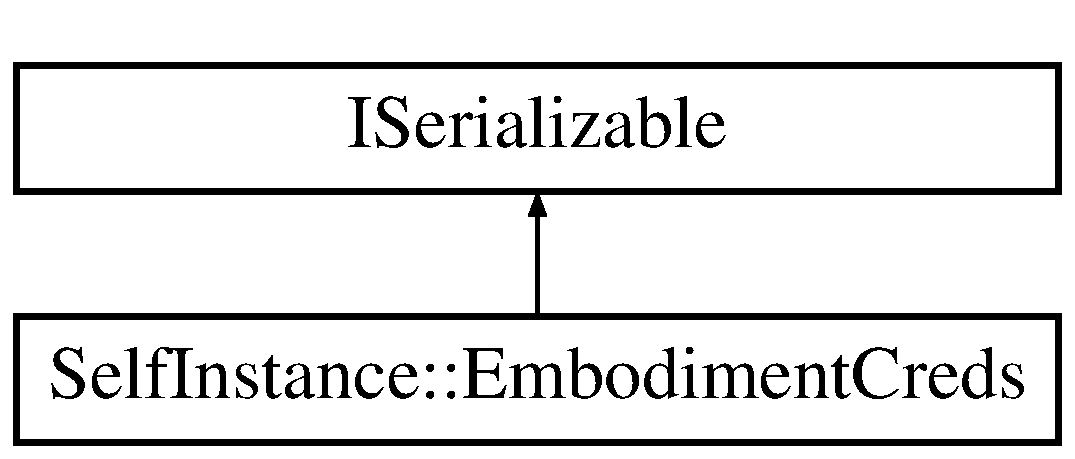
\includegraphics[height=2.000000cm]{struct_self_instance_1_1_embodiment_creds}
\end{center}
\end{figure}
\subsection*{Public Member Functions}
\begin{DoxyCompactItemize}
\item 
\mbox{\Hypertarget{struct_self_instance_1_1_embodiment_creds_a7cc3466ec2599fcd3b0fc7fead37c192}\label{struct_self_instance_1_1_embodiment_creds_a7cc3466ec2599fcd3b0fc7fead37c192}} 
{\bfseries R\+T\+T\+I\+\_\+\+D\+E\+CL} ()
\item 
\mbox{\Hypertarget{struct_self_instance_1_1_embodiment_creds_a10bbd6007d6aab5e0d1ca5cc779c3a70}\label{struct_self_instance_1_1_embodiment_creds_a10bbd6007d6aab5e0d1ca5cc779c3a70}} 
virtual void {\bfseries Serialize} (Json\+::\+Value \&json)
\item 
\mbox{\Hypertarget{struct_self_instance_1_1_embodiment_creds_a99bb8a19d9523161b19ddc1b62563748}\label{struct_self_instance_1_1_embodiment_creds_a99bb8a19d9523161b19ddc1b62563748}} 
virtual void {\bfseries Deserialize} (const Json\+::\+Value \&json)
\end{DoxyCompactItemize}
\subsection*{Public Attributes}
\begin{DoxyCompactItemize}
\item 
\mbox{\Hypertarget{struct_self_instance_1_1_embodiment_creds_a14fcc7ff988602dae9d35193a6b4bca3}\label{struct_self_instance_1_1_embodiment_creds_a14fcc7ff988602dae9d35193a6b4bca3}} 
std\+::string {\bfseries m\+\_\+\+Bearer\+Token}
\item 
\mbox{\Hypertarget{struct_self_instance_1_1_embodiment_creds_a504410b9d8768adaa47587f60af72257}\label{struct_self_instance_1_1_embodiment_creds_a504410b9d8768adaa47587f60af72257}} 
std\+::string {\bfseries m\+\_\+\+Group\+Id}
\item 
\mbox{\Hypertarget{struct_self_instance_1_1_embodiment_creds_a6f71b45ec9eac461e15e5b83bc8b5003}\label{struct_self_instance_1_1_embodiment_creds_a6f71b45ec9eac461e15e5b83bc8b5003}} 
std\+::string {\bfseries m\+\_\+\+Org\+Id}
\end{DoxyCompactItemize}


The documentation for this struct was generated from the following file\+:\begin{DoxyCompactItemize}
\item 
src/Self\+Instance.\+h\end{DoxyCompactItemize}

\hypertarget{class_emotion_agent}{}\section{Emotion\+Agent Class Reference}
\label{class_emotion_agent}\index{Emotion\+Agent@{Emotion\+Agent}}


This agent handles emotions.  




{\ttfamily \#include $<$Emotion\+Agent.\+h$>$}

Inheritance diagram for Emotion\+Agent\+:\begin{figure}[H]
\begin{center}
\leavevmode
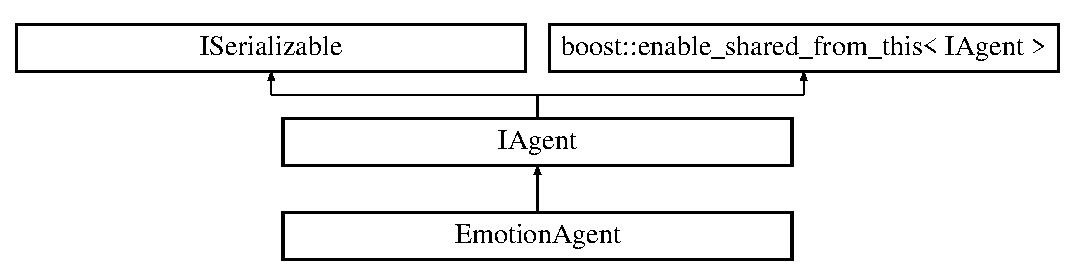
\includegraphics[height=3.000000cm]{class_emotion_agent}
\end{center}
\end{figure}
\subsection*{Classes}
\begin{DoxyCompactItemize}
\item 
struct \hyperlink{struct_emotion_agent_1_1_touch_response}{Touch\+Response}
\end{DoxyCompactItemize}
\subsection*{Public Types}
\begin{DoxyCompactItemize}
\item 
\mbox{\Hypertarget{class_emotion_agent_a1578745a702913f10ace02142df6163f}\label{class_emotion_agent_a1578745a702913f10ace02142df6163f}} 
typedef std\+::vector$<$ I\+Conditional\+::\+SP $>$ \hyperlink{class_emotion_agent_a1578745a702913f10ace02142df6163f}{Conditions}
\begin{DoxyCompactList}\small\item\em Types. \end{DoxyCompactList}\end{DoxyCompactItemize}
\subsection*{Public Member Functions}
\begin{DoxyCompactItemize}
\item 
\mbox{\Hypertarget{class_emotion_agent_a1f7279e7c1fc07df109c947794734814}\label{class_emotion_agent_a1f7279e7c1fc07df109c947794734814}} 
{\bfseries R\+T\+T\+I\+\_\+\+D\+E\+CL} ()
\item 
\mbox{\Hypertarget{class_emotion_agent_a74570ffbdf84d550a482b2a3b9b88c1d}\label{class_emotion_agent_a74570ffbdf84d550a482b2a3b9b88c1d}} 
\hyperlink{class_emotion_agent_a74570ffbdf84d550a482b2a3b9b88c1d}{Emotion\+Agent} ()
\begin{DoxyCompactList}\small\item\em Constructions. \end{DoxyCompactList}\item 
\mbox{\Hypertarget{class_emotion_agent_a423209e01aa9d2823317a0a5af3f468b}\label{class_emotion_agent_a423209e01aa9d2823317a0a5af3f468b}} 
virtual void \hyperlink{class_emotion_agent_a423209e01aa9d2823317a0a5af3f468b}{Serialize} (Json\+::\+Value \&json)
\begin{DoxyCompactList}\small\item\em I\+Serializable interface. \end{DoxyCompactList}\item 
\mbox{\Hypertarget{class_emotion_agent_a754713b176cf292986405269336b9541}\label{class_emotion_agent_a754713b176cf292986405269336b9541}} 
virtual void {\bfseries Deserialize} (const Json\+::\+Value \&json)
\item 
\mbox{\Hypertarget{class_emotion_agent_a366a230b7ea3926a4b899cabb6476512}\label{class_emotion_agent_a366a230b7ea3926a4b899cabb6476512}} 
virtual bool \hyperlink{class_emotion_agent_a366a230b7ea3926a4b899cabb6476512}{On\+Start} ()
\begin{DoxyCompactList}\small\item\em \hyperlink{class_i_agent}{I\+Agent} interface. \end{DoxyCompactList}\item 
\mbox{\Hypertarget{class_emotion_agent_a991e85bfd0583a70e8668cd4388bbfb1}\label{class_emotion_agent_a991e85bfd0583a70e8668cd4388bbfb1}} 
virtual bool {\bfseries On\+Stop} ()
\item 
\mbox{\Hypertarget{class_emotion_agent_a7fb8bdf10868cb62af2b849282db8a0f}\label{class_emotion_agent_a7fb8bdf10868cb62af2b849282db8a0f}} 
const float {\bfseries Get\+Emotional\+State} () const
\end{DoxyCompactItemize}
\subsection*{Additional Inherited Members}


\subsection{Detailed Description}
This agent handles emotions. 

The documentation for this class was generated from the following files\+:\begin{DoxyCompactItemize}
\item 
src/agent/Emotion\+Agent.\+h\item 
src/agent/Emotion\+Agent.\+cpp\end{DoxyCompactItemize}

\hypertarget{class_entity}{}\section{Entity Class Reference}
\label{class_entity}\index{Entity@{Entity}}


An entity object classified from Visual Recognition.  




{\ttfamily \#include $<$Entity.\+h$>$}

Inheritance diagram for Entity\+:\begin{figure}[H]
\begin{center}
\leavevmode
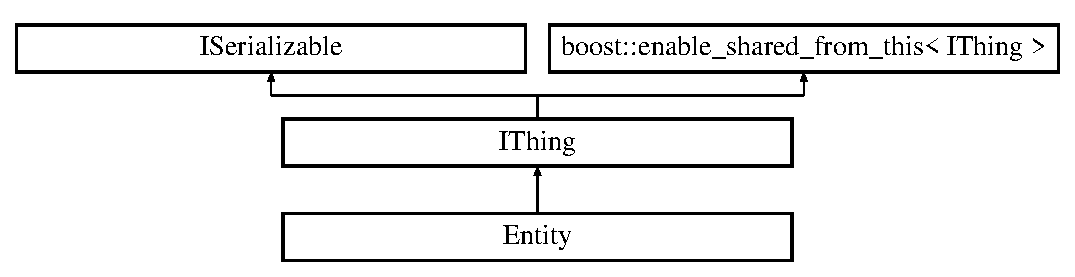
\includegraphics[height=3.000000cm]{class_entity}
\end{center}
\end{figure}
\subsection*{Public Types}
\begin{DoxyCompactItemize}
\item 
\mbox{\Hypertarget{class_entity_a7ec71d8cbb17276eb23575040bfbd481}\label{class_entity_a7ec71d8cbb17276eb23575040bfbd481}} 
typedef boost\+::shared\+\_\+ptr$<$ \hyperlink{class_entity}{Entity} $>$ \hyperlink{class_entity_a7ec71d8cbb17276eb23575040bfbd481}{SP}
\begin{DoxyCompactList}\small\item\em Types. \end{DoxyCompactList}\item 
\mbox{\Hypertarget{class_entity_a4cfc4e9d54917f65c04bcaa915d458df}\label{class_entity_a4cfc4e9d54917f65c04bcaa915d458df}} 
typedef boost\+::weak\+\_\+ptr$<$ \hyperlink{class_entity}{Entity} $>$ {\bfseries WP}
\end{DoxyCompactItemize}
\subsection*{Public Member Functions}
\begin{DoxyCompactItemize}
\item 
\mbox{\Hypertarget{class_entity_aaf469281c2b86495bf400362eda6ef57}\label{class_entity_aaf469281c2b86495bf400362eda6ef57}} 
{\bfseries R\+T\+T\+I\+\_\+\+D\+E\+CL} ()
\item 
\mbox{\Hypertarget{class_entity_aa4b1144ee0a85240c58268bab6a02636}\label{class_entity_aa4b1144ee0a85240c58268bab6a02636}} 
const std\+::string \& {\bfseries Get\+Top\+Class} () const
\item 
\mbox{\Hypertarget{class_entity_a9b114e718c3552a822a29cf0b3680fb3}\label{class_entity_a9b114e718c3552a822a29cf0b3680fb3}} 
const double \& {\bfseries Get\+Top\+Score} () const
\item 
\mbox{\Hypertarget{class_entity_a9de188785e8ec974fd587963b181f0fd}\label{class_entity_a9de188785e8ec974fd587963b181f0fd}} 
const std\+::string \& {\bfseries Get\+Type\+Heirarchy} () const
\item 
\mbox{\Hypertarget{class_entity_acb89eda6c2d05419ff158c54ad82afb3}\label{class_entity_acb89eda6c2d05419ff158c54ad82afb3}} 
void {\bfseries Set\+Top\+Class} (const std\+::string \&a\+\_\+\+Top\+Class)
\item 
\mbox{\Hypertarget{class_entity_a88c543a1bb48ca08676d992e521da246}\label{class_entity_a88c543a1bb48ca08676d992e521da246}} 
void {\bfseries Set\+Top\+Score} (const double \&a\+\_\+\+Top\+Score)
\item 
\mbox{\Hypertarget{class_entity_aaf6a72657088c2848e4f6c257d3d04d7}\label{class_entity_aaf6a72657088c2848e4f6c257d3d04d7}} 
void {\bfseries Set\+Type\+Hierarchy} (const std\+::string \&a\+\_\+\+Type\+Hierarchy)
\item 
\mbox{\Hypertarget{class_entity_af6d9b40f72df44d26108e44a94ca3be0}\label{class_entity_af6d9b40f72df44d26108e44a94ca3be0}} 
virtual void \hyperlink{class_entity_af6d9b40f72df44d26108e44a94ca3be0}{Serialize} (Json\+::\+Value \&json)
\begin{DoxyCompactList}\small\item\em I\+Serializable interface. \end{DoxyCompactList}\item 
\mbox{\Hypertarget{class_entity_aa26ea4f3da292a6903d54a0482ad5136}\label{class_entity_aa26ea4f3da292a6903d54a0482ad5136}} 
virtual void {\bfseries Deserialize} (const Json\+::\+Value \&json)
\end{DoxyCompactItemize}
\subsection*{Additional Inherited Members}


\subsection{Detailed Description}
An entity object classified from Visual Recognition. 

The documentation for this class was generated from the following files\+:\begin{DoxyCompactItemize}
\item 
src/blackboard/Entity.\+h\item 
src/blackboard/Entity.\+cpp\end{DoxyCompactItemize}

\hypertarget{class_environment}{}\section{Environment Class Reference}
\label{class_environment}\index{Environment@{Environment}}
Inheritance diagram for Environment\+:\begin{figure}[H]
\begin{center}
\leavevmode
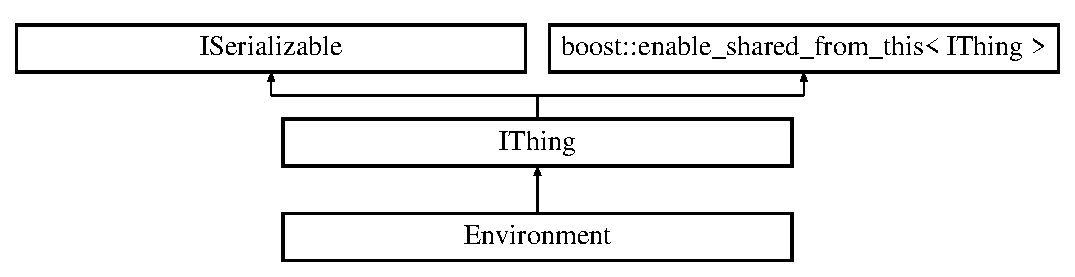
\includegraphics[height=3.000000cm]{class_environment}
\end{center}
\end{figure}
\subsection*{Public Types}
\begin{DoxyCompactItemize}
\item 
\mbox{\Hypertarget{class_environment_aedaf5e37c31f4aaab9d9b04b15000181}\label{class_environment_aedaf5e37c31f4aaab9d9b04b15000181}} 
typedef boost\+::shared\+\_\+ptr$<$ \hyperlink{class_environment}{Environment} $>$ \hyperlink{class_environment_aedaf5e37c31f4aaab9d9b04b15000181}{SP}
\begin{DoxyCompactList}\small\item\em Types. \end{DoxyCompactList}\item 
\mbox{\Hypertarget{class_environment_a026424718965a2c1e5b8e9f296af6266}\label{class_environment_a026424718965a2c1e5b8e9f296af6266}} 
typedef boost\+::weak\+\_\+ptr$<$ \hyperlink{class_environment}{Environment} $>$ {\bfseries WP}
\end{DoxyCompactItemize}
\subsection*{Public Member Functions}
\begin{DoxyCompactItemize}
\item 
\mbox{\Hypertarget{class_environment_a5129bc938599c31f0471ccd4b2e065f2}\label{class_environment_a5129bc938599c31f0471ccd4b2e065f2}} 
{\bfseries R\+T\+T\+I\+\_\+\+D\+E\+CL} ()
\item 
\mbox{\Hypertarget{class_environment_aa25092a73326ea28d175fe7e9e63dfb2}\label{class_environment_aa25092a73326ea28d175fe7e9e63dfb2}} 
const int \& {\bfseries Get\+Carbon\+Dioxide} () const
\item 
\mbox{\Hypertarget{class_environment_a0c37e68c4dbb1165c569610abd4d3001}\label{class_environment_a0c37e68c4dbb1165c569610abd4d3001}} 
const int \& {\bfseries Get\+Humidity} () const
\item 
\mbox{\Hypertarget{class_environment_a617b45e74b14d60fc67c58c5545d92c0}\label{class_environment_a617b45e74b14d60fc67c58c5545d92c0}} 
const float \& {\bfseries Get\+Temperature} () const
\item 
\mbox{\Hypertarget{class_environment_ac2efbab6db1444c9e778356d71b07093}\label{class_environment_ac2efbab6db1444c9e778356d71b07093}} 
const float \& {\bfseries Get\+Pressure} () const
\item 
\mbox{\Hypertarget{class_environment_a3f0a159e23a307abf67c55aae968676b}\label{class_environment_a3f0a159e23a307abf67c55aae968676b}} 
void {\bfseries Set\+Carbon\+Dioxide} (const int \&a\+\_\+\+Carbon\+Dioxide)
\item 
\mbox{\Hypertarget{class_environment_a90195dc8013a17d812dd5f2d196b675f}\label{class_environment_a90195dc8013a17d812dd5f2d196b675f}} 
void {\bfseries Set\+Humidity} (const int \&a\+\_\+\+Humidity)
\item 
\mbox{\Hypertarget{class_environment_acd735f2cc81c89b5577cd505f9581041}\label{class_environment_acd735f2cc81c89b5577cd505f9581041}} 
void {\bfseries Set\+Temperature} (const float \&a\+\_\+\+Temperature)
\item 
\mbox{\Hypertarget{class_environment_a5fd108e8eb46a4064c9f0fb1e9081378}\label{class_environment_a5fd108e8eb46a4064c9f0fb1e9081378}} 
void {\bfseries Set\+Pressure} (const float \&a\+\_\+\+Pressure)
\item 
\mbox{\Hypertarget{class_environment_a224cbba6df23fc2dc519642cec1324a6}\label{class_environment_a224cbba6df23fc2dc519642cec1324a6}} 
bool \hyperlink{class_environment_a224cbba6df23fc2dc519642cec1324a6}{Create} (const Json\+::\+Value \&json)
\begin{DoxyCompactList}\small\item\em Create this object from a J\+S\+ON response from a \hyperlink{class_remote_device}{Remote\+Device}. \end{DoxyCompactList}\item 
\mbox{\Hypertarget{class_environment_ad8e3b7d748f8bbc152ad52c4b180cd05}\label{class_environment_ad8e3b7d748f8bbc152ad52c4b180cd05}} 
virtual void \hyperlink{class_environment_ad8e3b7d748f8bbc152ad52c4b180cd05}{Serialize} (Json\+::\+Value \&json)
\begin{DoxyCompactList}\small\item\em I\+Serializable interface. \end{DoxyCompactList}\item 
\mbox{\Hypertarget{class_environment_abcc857ccb97d4e9540436f940145552b}\label{class_environment_abcc857ccb97d4e9540436f940145552b}} 
virtual void {\bfseries Deserialize} (const Json\+::\+Value \&json)
\end{DoxyCompactItemize}
\subsection*{Additional Inherited Members}


The documentation for this class was generated from the following files\+:\begin{DoxyCompactItemize}
\item 
src/blackboard/Environment.\+h\item 
src/blackboard/Environment.\+cpp\end{DoxyCompactItemize}

\hypertarget{class_environment_classifier}{}\section{Environment\+Classifier Class Reference}
\label{class_environment_classifier}\index{Environment\+Classifier@{Environment\+Classifier}}
Inheritance diagram for Environment\+Classifier\+:\begin{figure}[H]
\begin{center}
\leavevmode
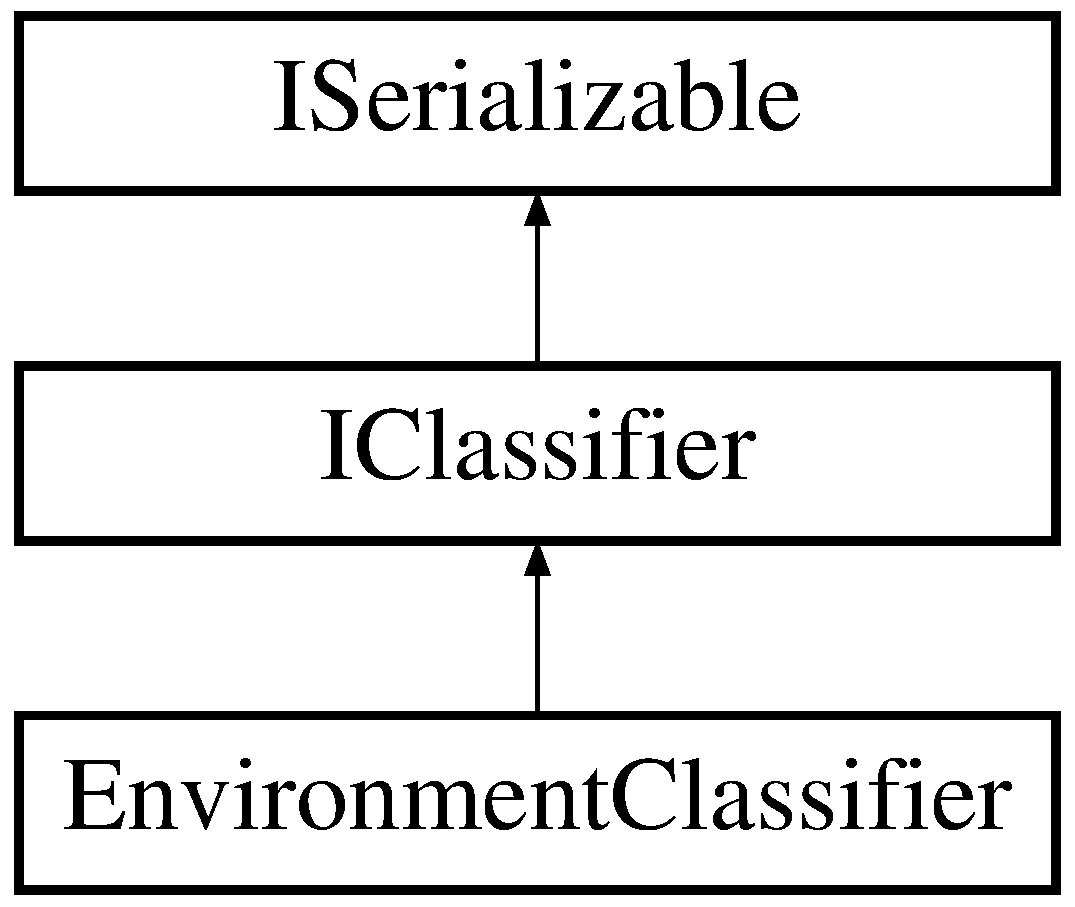
\includegraphics[height=3.000000cm]{class_environment_classifier}
\end{center}
\end{figure}
\subsection*{Public Member Functions}
\begin{DoxyCompactItemize}
\item 
\mbox{\Hypertarget{class_environment_classifier_aa1100572663bab6bbafedc200608f706}\label{class_environment_classifier_aa1100572663bab6bbafedc200608f706}} 
{\bfseries R\+T\+T\+I\+\_\+\+D\+E\+CL} ()
\item 
\mbox{\Hypertarget{class_environment_classifier_ae5bb06026ec04f98e28678f3d77a08af}\label{class_environment_classifier_ae5bb06026ec04f98e28678f3d77a08af}} 
virtual void \hyperlink{class_environment_classifier_ae5bb06026ec04f98e28678f3d77a08af}{Serialize} (Json\+::\+Value \&json)
\begin{DoxyCompactList}\small\item\em I\+Serializable interface. \end{DoxyCompactList}\item 
\mbox{\Hypertarget{class_environment_classifier_a0b931ec5425106247d5ff5778180f836}\label{class_environment_classifier_a0b931ec5425106247d5ff5778180f836}} 
virtual void {\bfseries Deserialize} (const Json\+::\+Value \&json)
\item 
\mbox{\Hypertarget{class_environment_classifier_aac33f8bcfc45591b27f3996ca1a722ee}\label{class_environment_classifier_aac33f8bcfc45591b27f3996ca1a722ee}} 
virtual const char $\ast$ \hyperlink{class_environment_classifier_aac33f8bcfc45591b27f3996ca1a722ee}{Get\+Name} () const
\begin{DoxyCompactList}\small\item\em \hyperlink{class_i_classifier}{I\+Classifier} interface. \end{DoxyCompactList}\item 
\mbox{\Hypertarget{class_environment_classifier_a77159420f0f565b85aa15cdeb9234064}\label{class_environment_classifier_a77159420f0f565b85aa15cdeb9234064}} 
virtual bool {\bfseries On\+Start} ()
\item 
\mbox{\Hypertarget{class_environment_classifier_a45c9d0b951c667fde24517c7006fd92d}\label{class_environment_classifier_a45c9d0b951c667fde24517c7006fd92d}} 
virtual bool {\bfseries On\+Stop} ()
\end{DoxyCompactItemize}
\subsection*{Additional Inherited Members}


The documentation for this class was generated from the following files\+:\begin{DoxyCompactItemize}
\item 
src/classifiers/Environment\+Classifier.\+h\item 
src/classifiers/Environment\+Classifier.\+cpp\end{DoxyCompactItemize}

\hypertarget{struct_graph_connector_1_1_event_request}{}\section{Graph\+Connector\+:\+:Event\+Request$<$ T $>$ Struct Template Reference}
\label{struct_graph_connector_1_1_event_request}\index{Graph\+Connector\+::\+Event\+Request$<$ T $>$@{Graph\+Connector\+::\+Event\+Request$<$ T $>$}}
Inheritance diagram for Graph\+Connector\+:\+:Event\+Request$<$ T $>$\+:\begin{figure}[H]
\begin{center}
\leavevmode
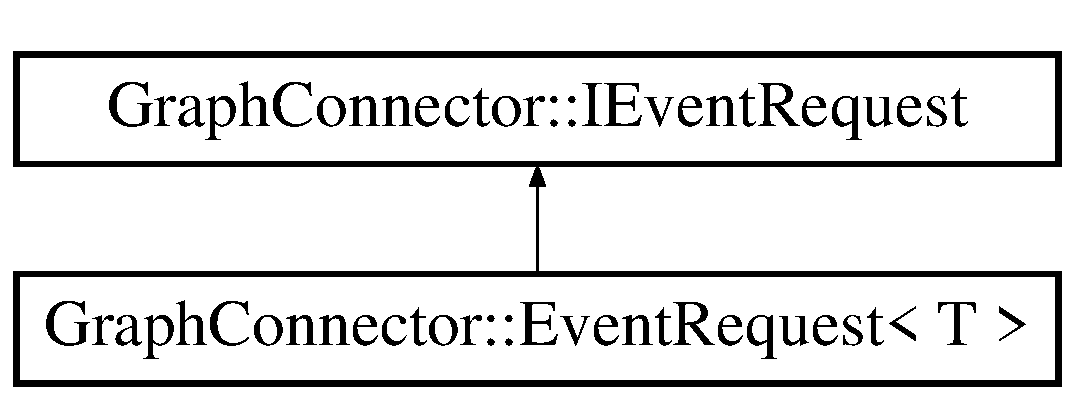
\includegraphics[height=2.000000cm]{struct_graph_connector_1_1_event_request}
\end{center}
\end{figure}
\subsection*{Public Member Functions}
\begin{DoxyCompactItemize}
\item 
\mbox{\Hypertarget{struct_graph_connector_1_1_event_request_a5a97eecb5aa1ed4b230888ca377516bf}\label{struct_graph_connector_1_1_event_request_a5a97eecb5aa1ed4b230888ca377516bf}} 
{\bfseries Event\+Request} (\hyperlink{class_graph_connector}{Graph\+Connector} $\ast$a\+\_\+p\+Connector, Event\+Id a\+\_\+n\+Event\+Id, Delegate$<$ T $>$ a\+\_\+\+Callback, T a\+\_\+\+Callback\+Arg, float a\+\_\+f\+Timeout)
\item 
\mbox{\Hypertarget{struct_graph_connector_1_1_event_request_ad1769de9927b0e896ced493d91aaaffe}\label{struct_graph_connector_1_1_event_request_ad1769de9927b0e896ced493d91aaaffe}} 
virtual void {\bfseries On\+Event\+Done} ()
\item 
\mbox{\Hypertarget{struct_graph_connector_1_1_event_request_a60e77ff91a97ad27ad674605d57a9167}\label{struct_graph_connector_1_1_event_request_a60e77ff91a97ad27ad674605d57a9167}} 
virtual void {\bfseries On\+Event\+Timeout} ()
\end{DoxyCompactItemize}
\subsection*{Public Attributes}
\begin{DoxyCompactItemize}
\item 
\mbox{\Hypertarget{struct_graph_connector_1_1_event_request_af1f109a752d53a28c5ecc43026158855}\label{struct_graph_connector_1_1_event_request_af1f109a752d53a28c5ecc43026158855}} 
\hyperlink{class_graph_connector}{Graph\+Connector} $\ast$ {\bfseries m\+\_\+p\+Connector}
\item 
\mbox{\Hypertarget{struct_graph_connector_1_1_event_request_aee2b279a9195229d124125b2d266d92d}\label{struct_graph_connector_1_1_event_request_aee2b279a9195229d124125b2d266d92d}} 
Event\+Id {\bfseries m\+\_\+n\+Event\+Id}
\item 
\mbox{\Hypertarget{struct_graph_connector_1_1_event_request_a4942a26334695f55f7a9cd87c6ffcae2}\label{struct_graph_connector_1_1_event_request_a4942a26334695f55f7a9cd87c6ffcae2}} 
Delegate$<$ T $>$ {\bfseries m\+\_\+\+Callback}
\item 
\mbox{\Hypertarget{struct_graph_connector_1_1_event_request_a982858032ba2886db41ac2df87726e0b}\label{struct_graph_connector_1_1_event_request_a982858032ba2886db41ac2df87726e0b}} 
T {\bfseries m\+\_\+\+Callback\+Arg}
\item 
\mbox{\Hypertarget{struct_graph_connector_1_1_event_request_ad189be88a7c5b85b51d81b7a20ca1879}\label{struct_graph_connector_1_1_event_request_ad189be88a7c5b85b51d81b7a20ca1879}} 
Timer\+Pool\+::\+I\+Timer\+::\+SP {\bfseries m\+\_\+sp\+Timer}
\end{DoxyCompactItemize}
\subsection*{Additional Inherited Members}


The documentation for this struct was generated from the following file\+:\begin{DoxyCompactItemize}
\item 
src/models/Graph\+Connector.\+h\end{DoxyCompactItemize}

\hypertarget{class_f2_beat_detect}{}\section{F2\+Beat\+Detect Class Reference}
\label{class_f2_beat_detect}\index{F2\+Beat\+Detect@{F2\+Beat\+Detect}}
Inheritance diagram for F2\+Beat\+Detect\+:\begin{figure}[H]
\begin{center}
\leavevmode
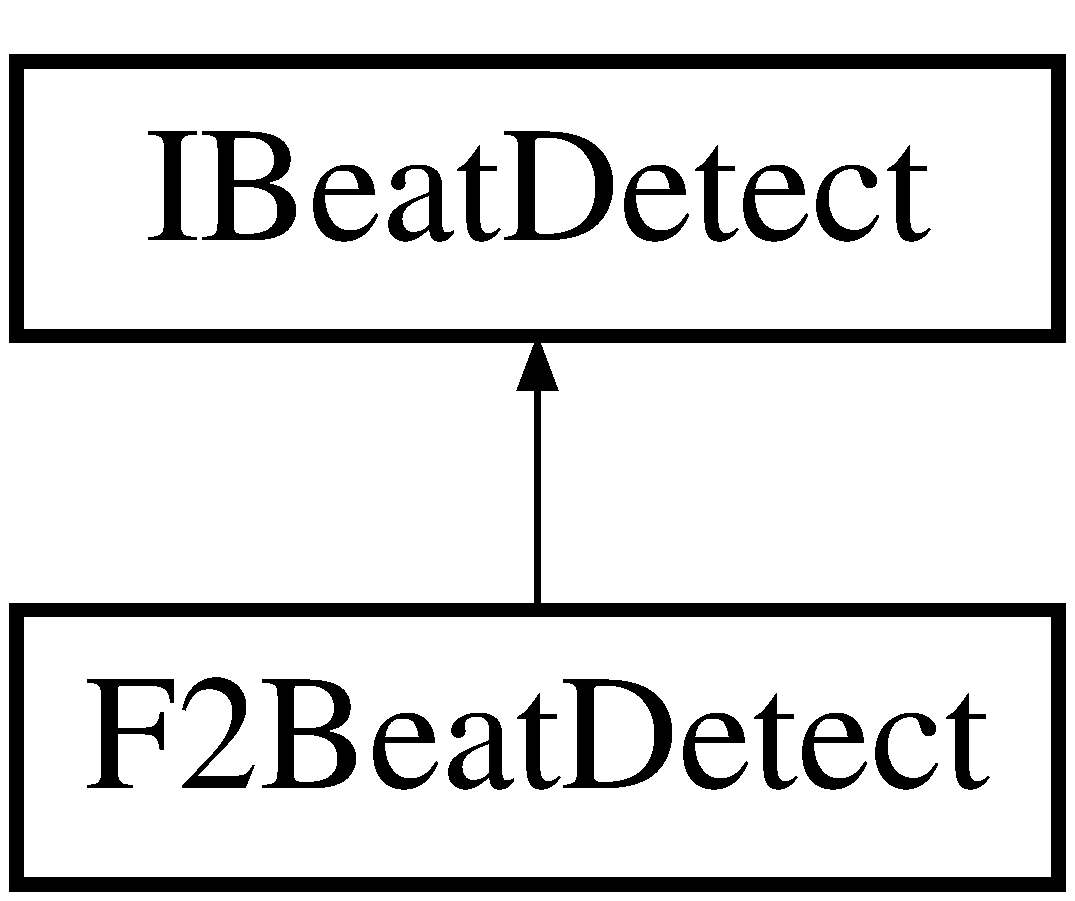
\includegraphics[height=2.000000cm]{class_f2_beat_detect}
\end{center}
\end{figure}
\subsection*{Public Member Functions}
\begin{DoxyCompactItemize}
\item 
\mbox{\Hypertarget{class_f2_beat_detect_ae727f17a85d525376aed6b8d22bfa9a4}\label{class_f2_beat_detect_ae727f17a85d525376aed6b8d22bfa9a4}} 
virtual void \hyperlink{class_f2_beat_detect_ae727f17a85d525376aed6b8d22bfa9a4}{Initialize} (int time\+Size, float sample\+Rate)
\begin{DoxyCompactList}\small\item\em Initialize this beat detector. \end{DoxyCompactList}\item 
\mbox{\Hypertarget{class_f2_beat_detect_afca1254f1c9f4b866d08dc5afb5bf367}\label{class_f2_beat_detect_afca1254f1c9f4b866d08dc5afb5bf367}} 
virtual void \hyperlink{class_f2_beat_detect_afca1254f1c9f4b866d08dc5afb5bf367}{Reset} ()
\begin{DoxyCompactList}\small\item\em Release this beat detector. \end{DoxyCompactList}\item 
\mbox{\Hypertarget{class_f2_beat_detect_a6a98eefb6041b575fba1d7255bb8491e}\label{class_f2_beat_detect_a6a98eefb6041b575fba1d7255bb8491e}} 
bool \hyperlink{class_f2_beat_detect_a6a98eefb6041b575fba1d7255bb8491e}{Detect} (std\+::vector$<$ float $>$ \&a\+\_\+\+Samples, size\+\_\+t a\+\_\+n\+Offset)
\begin{DoxyCompactList}\small\item\em Returns true if a onset is detected in this block of audio data. \end{DoxyCompactList}\end{DoxyCompactItemize}
\subsection*{Additional Inherited Members}


The documentation for this class was generated from the following files\+:\begin{DoxyCompactItemize}
\item 
src/utils/fft/F2\+Beat\+Detect.\+h\item 
src/utils/fft/F2\+Beat\+Detect.\+cpp\end{DoxyCompactItemize}

\hypertarget{class_face_classifier}{}\section{Face\+Classifier Class Reference}
\label{class_face_classifier}\index{Face\+Classifier@{Face\+Classifier}}


{\ttfamily \#include $<$Face\+Classifier.\+h$>$}

Inheritance diagram for Face\+Classifier\+:\begin{figure}[H]
\begin{center}
\leavevmode
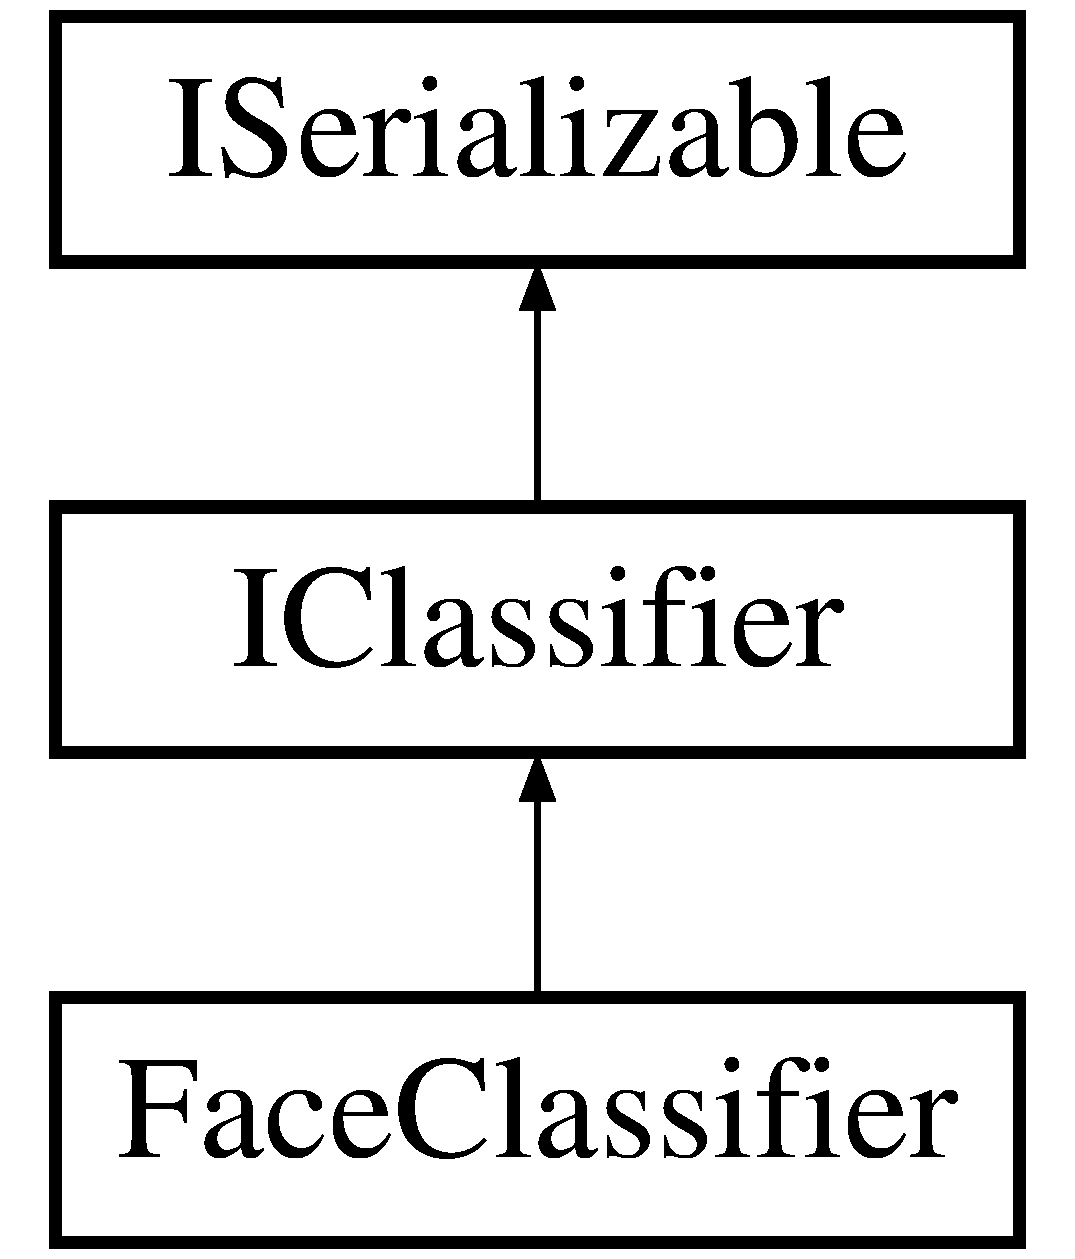
\includegraphics[height=3.000000cm]{class_face_classifier}
\end{center}
\end{figure}
\subsection*{Public Member Functions}
\begin{DoxyCompactItemize}
\item 
\mbox{\Hypertarget{class_face_classifier_ac8f91bc48109bf3c5f9f62ce4dfff6d1}\label{class_face_classifier_ac8f91bc48109bf3c5f9f62ce4dfff6d1}} 
{\bfseries R\+T\+T\+I\+\_\+\+D\+E\+CL} ()
\item 
\mbox{\Hypertarget{class_face_classifier_a7a88b6d79f427a05540e0f6b00b70ab4}\label{class_face_classifier_a7a88b6d79f427a05540e0f6b00b70ab4}} 
virtual void \hyperlink{class_face_classifier_a7a88b6d79f427a05540e0f6b00b70ab4}{Serialize} (Json\+::\+Value \&json)
\begin{DoxyCompactList}\small\item\em I\+Serializable interface. \end{DoxyCompactList}\item 
\mbox{\Hypertarget{class_face_classifier_af7b0a56809bb07fa4c96a0a4640fd4b0}\label{class_face_classifier_af7b0a56809bb07fa4c96a0a4640fd4b0}} 
virtual void {\bfseries Deserialize} (const Json\+::\+Value \&json)
\item 
\mbox{\Hypertarget{class_face_classifier_a5efcd3a958a7c00a6afabd864fe1bc66}\label{class_face_classifier_a5efcd3a958a7c00a6afabd864fe1bc66}} 
virtual const char $\ast$ \hyperlink{class_face_classifier_a5efcd3a958a7c00a6afabd864fe1bc66}{Get\+Name} () const
\begin{DoxyCompactList}\small\item\em \hyperlink{class_i_classifier}{I\+Classifier} interface. \end{DoxyCompactList}\item 
\mbox{\Hypertarget{class_face_classifier_a63467935351f6e31ffb297509a1ef2ce}\label{class_face_classifier_a63467935351f6e31ffb297509a1ef2ce}} 
virtual bool {\bfseries On\+Start} ()
\item 
\mbox{\Hypertarget{class_face_classifier_a8e3d1e7c0607b8530ca7042540a72894}\label{class_face_classifier_a8e3d1e7c0607b8530ca7042540a72894}} 
virtual bool {\bfseries On\+Stop} ()
\item 
\mbox{\Hypertarget{class_face_classifier_a7d9ee408b95543317637c8070dbf73be}\label{class_face_classifier_a7d9ee408b95543317637c8070dbf73be}} 
bool {\bfseries Learn\+Person} (const \hyperlink{class_person_a16426d961e9ca63d2524812444163d36}{Person\+::\+SP} \&a\+\_\+sp\+Person)
\end{DoxyCompactItemize}
\subsection*{Additional Inherited Members}


\subsection{Detailed Description}
This classifier subscribes to all video sensors and classifies all incoming video data which then adds a Concept to the \hyperlink{class_black_board}{Black\+Board}. 

The documentation for this class was generated from the following files\+:\begin{DoxyCompactItemize}
\item 
src/classifiers/Face\+Classifier.\+h\item 
src/classifiers/Face\+Classifier.\+cpp\end{DoxyCompactItemize}

\hypertarget{class_failure}{}\section{Failure Class Reference}
\label{class_failure}\index{Failure@{Failure}}
Inheritance diagram for Failure\+:\begin{figure}[H]
\begin{center}
\leavevmode
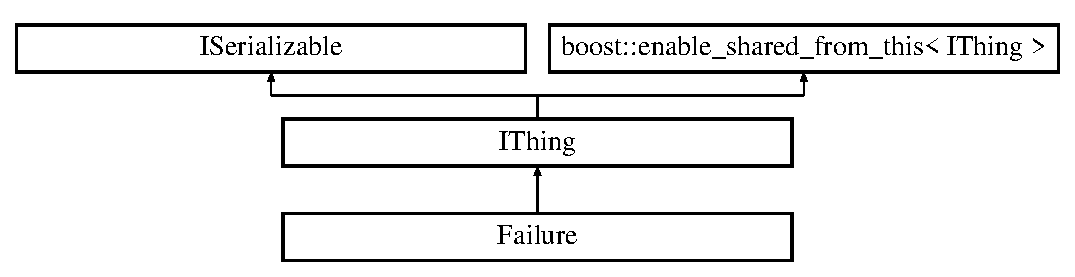
\includegraphics[height=3.000000cm]{class_failure}
\end{center}
\end{figure}
\subsection*{Public Types}
\begin{DoxyCompactItemize}
\item 
\mbox{\Hypertarget{class_failure_ac6f000b2607465cec6aab77983c7a615}\label{class_failure_ac6f000b2607465cec6aab77983c7a615}} 
typedef boost\+::shared\+\_\+ptr$<$ \hyperlink{class_failure}{Failure} $>$ \hyperlink{class_failure_ac6f000b2607465cec6aab77983c7a615}{SP}
\begin{DoxyCompactList}\small\item\em Types. \end{DoxyCompactList}\item 
\mbox{\Hypertarget{class_failure_acf76cbdbeeb671f63ff6401e5a9b2a83}\label{class_failure_acf76cbdbeeb671f63ff6401e5a9b2a83}} 
typedef boost\+::weak\+\_\+ptr$<$ \hyperlink{class_failure}{Failure} $>$ {\bfseries WP}
\end{DoxyCompactItemize}
\subsection*{Public Member Functions}
\begin{DoxyCompactItemize}
\item 
\mbox{\Hypertarget{class_failure_a1f27e78c4983c4db41563903d4a18b90}\label{class_failure_a1f27e78c4983c4db41563903d4a18b90}} 
{\bfseries R\+T\+T\+I\+\_\+\+D\+E\+CL} ()
\item 
\mbox{\Hypertarget{class_failure_afd1a1e0662adc20f77fc270ec1075fa8}\label{class_failure_afd1a1e0662adc20f77fc270ec1075fa8}} 
\hyperlink{class_failure_afd1a1e0662adc20f77fc270ec1075fa8}{Failure} ()
\begin{DoxyCompactList}\small\item\em Construction. \end{DoxyCompactList}\item 
\mbox{\Hypertarget{class_failure_ad70ad8aeb9a3aede78e8ee0da9cffefb}\label{class_failure_ad70ad8aeb9a3aede78e8ee0da9cffefb}} 
{\bfseries Failure} (const std\+::string \&a\+\_\+\+Name, const std\+::string \&a\+\_\+\+Info, double a\+\_\+\+Confidence, double a\+\_\+\+Threshold)
\item 
\mbox{\Hypertarget{class_failure_a0c02713afa6aaeea93b52e6de7282e10}\label{class_failure_a0c02713afa6aaeea93b52e6de7282e10}} 
virtual void \hyperlink{class_failure_a0c02713afa6aaeea93b52e6de7282e10}{Serialize} (Json\+::\+Value \&json)
\begin{DoxyCompactList}\small\item\em I\+Serializable. \end{DoxyCompactList}\item 
\mbox{\Hypertarget{class_failure_a677852817f33eeeb4b81294b421a0584}\label{class_failure_a677852817f33eeeb4b81294b421a0584}} 
virtual void {\bfseries Deserialize} (const Json\+::\+Value \&json)
\end{DoxyCompactItemize}
\subsection*{Additional Inherited Members}


The documentation for this class was generated from the following files\+:\begin{DoxyCompactItemize}
\item 
src/blackboard/Failure.\+h\item 
src/blackboard/Failure.\+cpp\end{DoxyCompactItemize}

\hypertarget{class_f_beat_detect}{}\section{F\+Beat\+Detect Class Reference}
\label{class_f_beat_detect}\index{F\+Beat\+Detect@{F\+Beat\+Detect}}
Inheritance diagram for F\+Beat\+Detect\+:\begin{figure}[H]
\begin{center}
\leavevmode
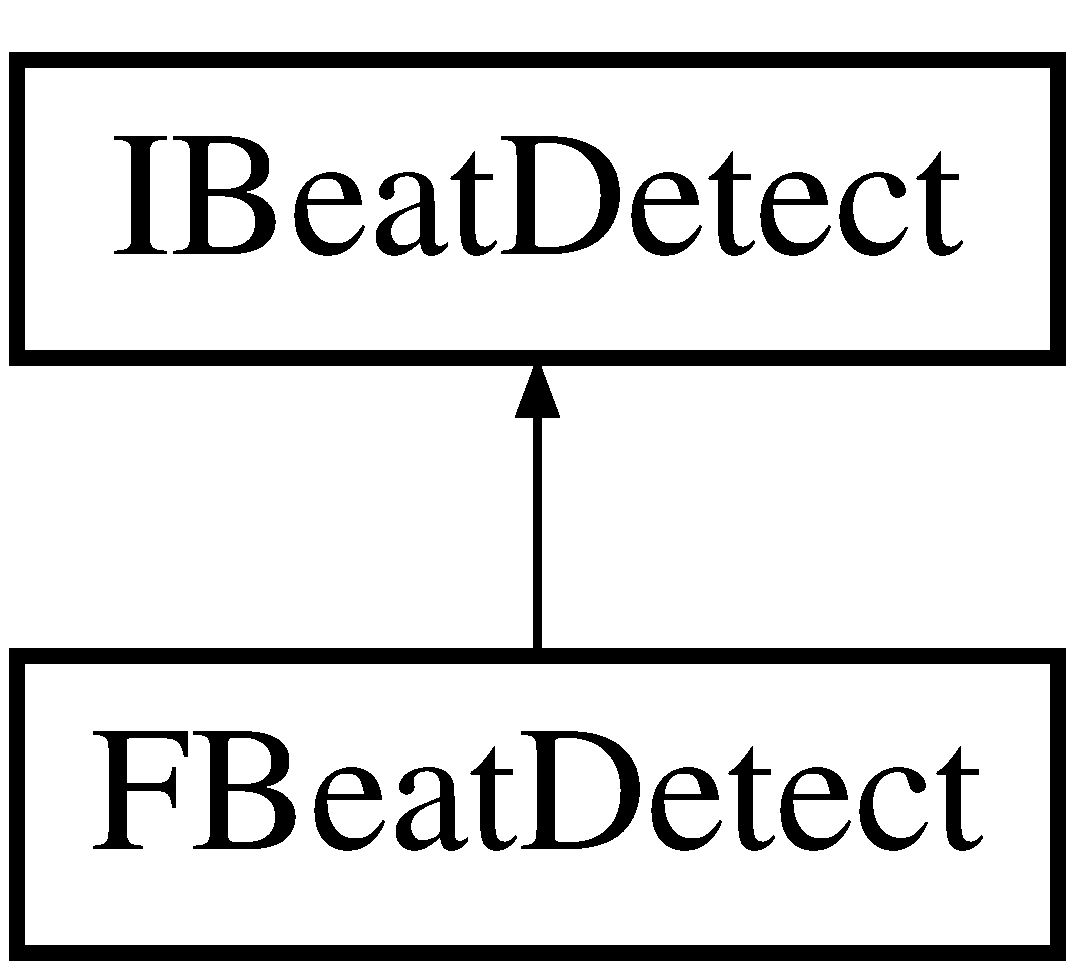
\includegraphics[height=2.000000cm]{class_f_beat_detect}
\end{center}
\end{figure}
\subsection*{Public Member Functions}
\begin{DoxyCompactItemize}
\item 
\mbox{\Hypertarget{class_f_beat_detect_a34a48d288ca04f08d4722dbff72252df}\label{class_f_beat_detect_a34a48d288ca04f08d4722dbff72252df}} 
virtual void \hyperlink{class_f_beat_detect_a34a48d288ca04f08d4722dbff72252df}{Initialize} (int time\+Size, float sample\+Rate)
\begin{DoxyCompactList}\small\item\em Initialize this beat detector. \end{DoxyCompactList}\item 
\mbox{\Hypertarget{class_f_beat_detect_a141db57cfa7acc2a45e77ac28c970776}\label{class_f_beat_detect_a141db57cfa7acc2a45e77ac28c970776}} 
virtual void \hyperlink{class_f_beat_detect_a141db57cfa7acc2a45e77ac28c970776}{Reset} ()
\begin{DoxyCompactList}\small\item\em Release this beat detector. \end{DoxyCompactList}\item 
\mbox{\Hypertarget{class_f_beat_detect_ad6298d38e6ac967abeb1dec8f0339e1d}\label{class_f_beat_detect_ad6298d38e6ac967abeb1dec8f0339e1d}} 
bool \hyperlink{class_f_beat_detect_ad6298d38e6ac967abeb1dec8f0339e1d}{Detect} (std\+::vector$<$ float $>$ \&a\+\_\+\+Samples, size\+\_\+t a\+\_\+n\+Offset)
\begin{DoxyCompactList}\small\item\em Returns true if a onset is detected in this block of audio data. \end{DoxyCompactList}\item 
\mbox{\Hypertarget{class_f_beat_detect_a5c892e74c4c1320a15fcaf6422b52417}\label{class_f_beat_detect_a5c892e74c4c1320a15fcaf6422b52417}} 
bool {\bfseries Is\+Onset} (int i) const
\item 
\mbox{\Hypertarget{class_f_beat_detect_af83d0ffedd3b071c8003628150c8ca82}\label{class_f_beat_detect_af83d0ffedd3b071c8003628150c8ca82}} 
bool {\bfseries Is\+Kick} () const
\item 
\mbox{\Hypertarget{class_f_beat_detect_a3a83abb2a3b152b01dc4405c7f77bcbd}\label{class_f_beat_detect_a3a83abb2a3b152b01dc4405c7f77bcbd}} 
bool {\bfseries Is\+Snare} () const
\item 
\mbox{\Hypertarget{class_f_beat_detect_ae2867a9c4a488ffba2556d9732a0e868}\label{class_f_beat_detect_ae2867a9c4a488ffba2556d9732a0e868}} 
bool {\bfseries Is\+Hat} () const
\item 
\mbox{\Hypertarget{class_f_beat_detect_a6f871db6cdeea7106ce2adbb676c053c}\label{class_f_beat_detect_a6f871db6cdeea7106ce2adbb676c053c}} 
bool {\bfseries Is\+Range} (int low, int high, int threshold) const
\end{DoxyCompactItemize}
\subsection*{Additional Inherited Members}


The documentation for this class was generated from the following files\+:\begin{DoxyCompactItemize}
\item 
src/utils/fft/F\+Beat\+Detect.\+h\item 
src/utils/fft/F\+Beat\+Detect.\+cpp\end{DoxyCompactItemize}

\hypertarget{class_feature_manager}{}\section{Feature\+Manager Class Reference}
\label{class_feature_manager}\index{Feature\+Manager@{Feature\+Manager}}


{\ttfamily \#include $<$Feature\+Manager.\+h$>$}

\subsection*{Public Types}
\begin{DoxyCompactItemize}
\item 
\mbox{\Hypertarget{class_feature_manager_ac5e551b04984aaab5e31391e934208bb}\label{class_feature_manager_ac5e551b04984aaab5e31391e934208bb}} 
typedef std\+::list$<$ \hyperlink{class_i_feature_extractor_accaef91768ee64d51b4dc959f36e9f08}{I\+Feature\+Extractor\+::\+SP} $>$ \hyperlink{class_feature_manager_ac5e551b04984aaab5e31391e934208bb}{Feature\+Extractor\+List}
\begin{DoxyCompactList}\small\item\em Types. \end{DoxyCompactList}\item 
\mbox{\Hypertarget{class_feature_manager_a8d757b7e1c0e8a173e42981a79898b73}\label{class_feature_manager_a8d757b7e1c0e8a173e42981a79898b73}} 
typedef Factory$<$ \hyperlink{class_i_feature_extractor}{I\+Feature\+Extractor} $>$ {\bfseries Feature\+Extractor\+Factory}
\end{DoxyCompactItemize}
\subsection*{Public Member Functions}
\begin{DoxyCompactItemize}
\item 
\mbox{\Hypertarget{class_feature_manager_a4e0ef0a55579bdaefc85970cb492b1bb}\label{class_feature_manager_a4e0ef0a55579bdaefc85970cb492b1bb}} 
\hyperlink{class_feature_manager_a4e0ef0a55579bdaefc85970cb492b1bb}{Feature\+Manager} ()
\begin{DoxyCompactList}\small\item\em Construction. \end{DoxyCompactList}\item 
\mbox{\Hypertarget{class_feature_manager_a365f702520b97592e1abff59eb907f2b}\label{class_feature_manager_a365f702520b97592e1abff59eb907f2b}} 
const \hyperlink{class_feature_manager_ac5e551b04984aaab5e31391e934208bb}{Feature\+Extractor\+List} \& \hyperlink{class_feature_manager_a365f702520b97592e1abff59eb907f2b}{Get\+Feature\+Extractor\+List} () const
\begin{DoxyCompactList}\small\item\em Accessors. \end{DoxyCompactList}\item 
\mbox{\Hypertarget{class_feature_manager_ae22e14ad392ba3a7e23dccb40e7da30a}\label{class_feature_manager_ae22e14ad392ba3a7e23dccb40e7da30a}} 
bool \hyperlink{class_feature_manager_ae22e14ad392ba3a7e23dccb40e7da30a}{Start} ()
\begin{DoxyCompactList}\small\item\em Start this manager, initializes all available Classifer objects. \end{DoxyCompactList}\item 
\mbox{\Hypertarget{class_feature_manager_aa84b4f17c9b92744ff06e4f92fe92904}\label{class_feature_manager_aa84b4f17c9b92744ff06e4f92fe92904}} 
bool \hyperlink{class_feature_manager_aa84b4f17c9b92744ff06e4f92fe92904}{Stop} ()
\begin{DoxyCompactList}\small\item\em Stop this manager. \end{DoxyCompactList}\item 
\mbox{\Hypertarget{class_feature_manager_a3e5e9a2474841c6fff77cd2c95598611}\label{class_feature_manager_a3e5e9a2474841c6fff77cd2c95598611}} 
{\footnotesize template$<$typename T $>$ }\\T $\ast$ {\bfseries Find\+Extractor} () const
\item 
\mbox{\Hypertarget{class_feature_manager_a0f82bb48dd79d49d62e083421165af34}\label{class_feature_manager_a0f82bb48dd79d49d62e083421165af34}} 
{\footnotesize template$<$typename T $>$ }\\T $\ast$ {\bfseries Get\+Extractor} ()
\end{DoxyCompactItemize}


\subsection{Detailed Description}
This feature manager manages all Feature extractors, those feature extractors push data into the Blackboard object. 

The documentation for this class was generated from the following files\+:\begin{DoxyCompactItemize}
\item 
src/extractors/Feature\+Manager.\+h\item 
src/extractors/Feature\+Manager.\+cpp\end{DoxyCompactItemize}

\hypertarget{class_feedback_agent}{}\section{Feedback\+Agent Class Reference}
\label{class_feedback_agent}\index{Feedback\+Agent@{Feedback\+Agent}}
Inheritance diagram for Feedback\+Agent\+:\begin{figure}[H]
\begin{center}
\leavevmode
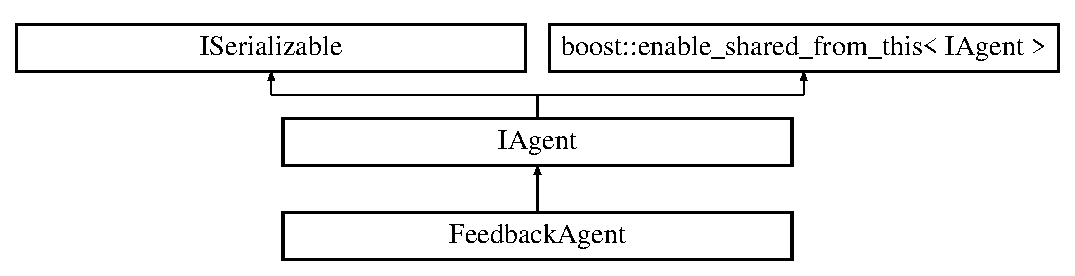
\includegraphics[height=3.000000cm]{class_feedback_agent}
\end{center}
\end{figure}
\subsection*{Public Member Functions}
\begin{DoxyCompactItemize}
\item 
\mbox{\Hypertarget{class_feedback_agent_a4b980f75d4844422e9115b712756d52f}\label{class_feedback_agent_a4b980f75d4844422e9115b712756d52f}} 
{\bfseries R\+T\+T\+I\+\_\+\+D\+E\+CL} ()
\item 
\mbox{\Hypertarget{class_feedback_agent_a1c2ba04c669c5de53307745e1f73ddfa}\label{class_feedback_agent_a1c2ba04c669c5de53307745e1f73ddfa}} 
virtual void \hyperlink{class_feedback_agent_a1c2ba04c669c5de53307745e1f73ddfa}{Serialize} (Json\+::\+Value \&json)
\begin{DoxyCompactList}\small\item\em I\+Serializable interface. \end{DoxyCompactList}\item 
\mbox{\Hypertarget{class_feedback_agent_a57332a70fb9818b9d0ae83a1d043c354}\label{class_feedback_agent_a57332a70fb9818b9d0ae83a1d043c354}} 
virtual void {\bfseries Deserialize} (const Json\+::\+Value \&json)
\item 
\mbox{\Hypertarget{class_feedback_agent_a76f85c5c893229b493b53a67fc4cf54f}\label{class_feedback_agent_a76f85c5c893229b493b53a67fc4cf54f}} 
virtual bool \hyperlink{class_feedback_agent_a76f85c5c893229b493b53a67fc4cf54f}{On\+Start} ()
\begin{DoxyCompactList}\small\item\em \hyperlink{class_i_agent}{I\+Agent} interface. \end{DoxyCompactList}\item 
\mbox{\Hypertarget{class_feedback_agent_ad9a3c839cb4b945f955cda57cb7659b2}\label{class_feedback_agent_ad9a3c839cb4b945f955cda57cb7659b2}} 
virtual bool {\bfseries On\+Stop} ()
\end{DoxyCompactItemize}
\subsection*{Additional Inherited Members}


The documentation for this class was generated from the following files\+:\begin{DoxyCompactItemize}
\item 
src/agent/Feedback\+Agent.\+h\item 
src/agent/Feedback\+Agent.\+cpp\end{DoxyCompactItemize}

\hypertarget{class_f_f_t}{}\section{F\+FT Class Reference}
\label{class_f_f_t}\index{F\+FT@{F\+FT}}
Inheritance diagram for F\+FT\+:\begin{figure}[H]
\begin{center}
\leavevmode
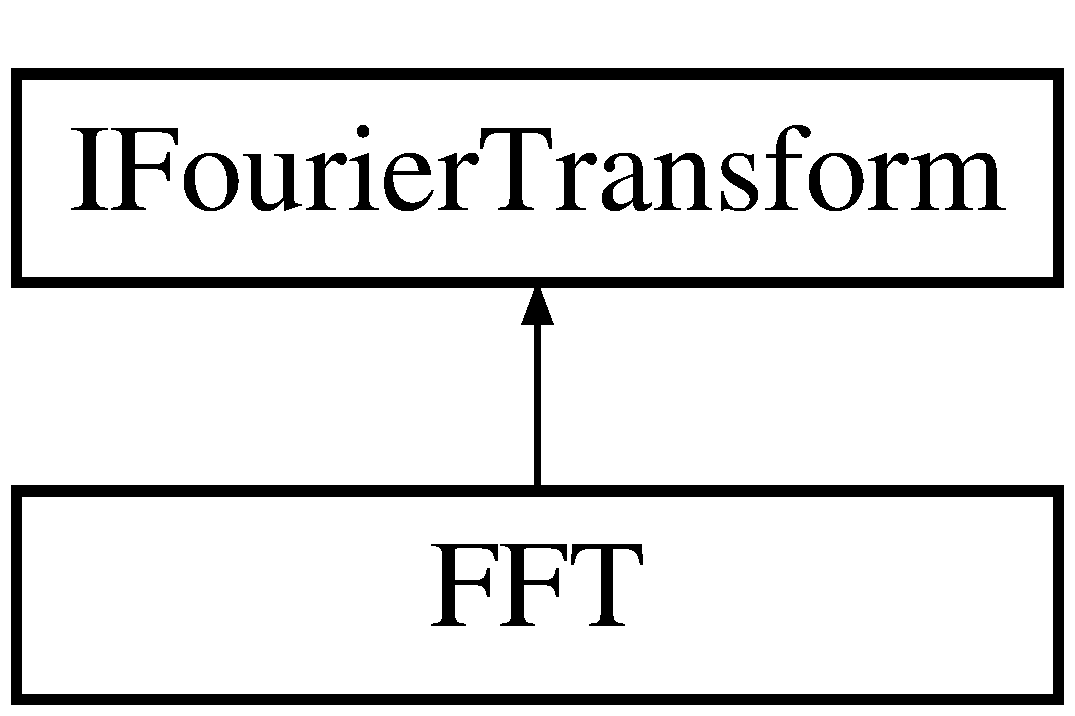
\includegraphics[height=2.000000cm]{class_f_f_t}
\end{center}
\end{figure}
\subsection*{Public Member Functions}
\begin{DoxyCompactItemize}
\item 
\mbox{\Hypertarget{class_f_f_t_a499bcf08055d90f0379fbb3b69932446}\label{class_f_f_t_a499bcf08055d90f0379fbb3b69932446}} 
void {\bfseries Initialize} (int a\+\_\+n\+Time\+Size, float a\+\_\+n\+Sample\+Rate, \hyperlink{class_i_window_function}{I\+Window\+Function} $\ast$a\+\_\+p\+Function=N\+U\+LL)
\item 
\mbox{\Hypertarget{class_f_f_t_ae244f8b8ea4d8d043ec42a699db05cb9}\label{class_f_f_t_ae244f8b8ea4d8d043ec42a699db05cb9}} 
virtual void \hyperlink{class_f_f_t_ae244f8b8ea4d8d043ec42a699db05cb9}{Allocate\+Arrays} ()
\begin{DoxyCompactList}\small\item\em Fourier\+Transform interface. \end{DoxyCompactList}\item 
\mbox{\Hypertarget{class_f_f_t_a367e2b06ea96c42fe012c477fd54132c}\label{class_f_f_t_a367e2b06ea96c42fe012c477fd54132c}} 
virtual void {\bfseries Scale\+Band} (int i, float s)
\item 
\mbox{\Hypertarget{class_f_f_t_a28af2a995d9d89baa54fbb9d6d0c8288}\label{class_f_f_t_a28af2a995d9d89baa54fbb9d6d0c8288}} 
virtual void {\bfseries Set\+Band} (int i, float a)
\item 
\mbox{\Hypertarget{class_f_f_t_a3ee9e4cd928bfbf181e3b79c2527b57a}\label{class_f_f_t_a3ee9e4cd928bfbf181e3b79c2527b57a}} 
virtual void {\bfseries Forward} (std\+::vector$<$ float $>$ \&a\+\_\+\+Samples, int a\+\_\+n\+Offset=0)
\item 
\mbox{\Hypertarget{class_f_f_t_aa6d8c765a1cd6a2b5913fb3605206bdc}\label{class_f_f_t_aa6d8c765a1cd6a2b5913fb3605206bdc}} 
virtual void {\bfseries Inverse} (std\+::vector$<$ float $>$ \&a\+\_\+\+Samples, int a\+\_\+n\+Offset=0)
\end{DoxyCompactItemize}
\subsection*{Additional Inherited Members}


The documentation for this class was generated from the following file\+:\begin{DoxyCompactItemize}
\item 
src/utils/fft/F\+F\+T.\+h\end{DoxyCompactItemize}

\hypertarget{class_graph_self_1_1_filter_traverser}{}\section{Graph\+Self\+:\+:Filter\+Traverser Class Reference}
\label{class_graph_self_1_1_filter_traverser}\index{Graph\+Self\+::\+Filter\+Traverser@{Graph\+Self\+::\+Filter\+Traverser}}
Inheritance diagram for Graph\+Self\+:\+:Filter\+Traverser\+:\begin{figure}[H]
\begin{center}
\leavevmode
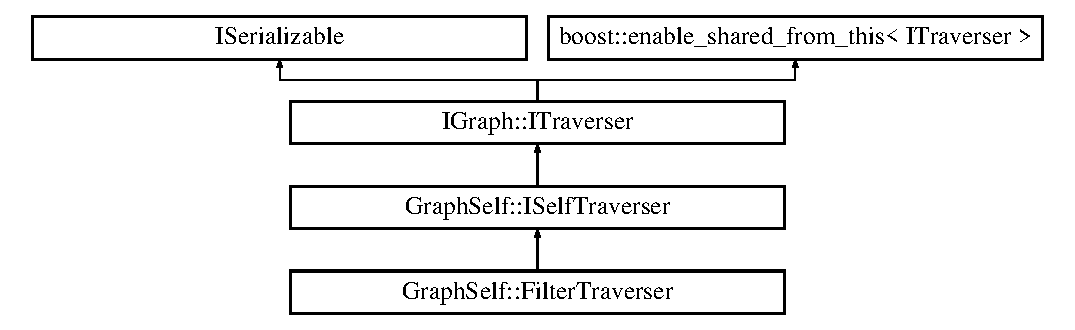
\includegraphics[height=3.985765cm]{class_graph_self_1_1_filter_traverser}
\end{center}
\end{figure}
\subsection*{Public Member Functions}
\begin{DoxyCompactItemize}
\item 
\mbox{\Hypertarget{class_graph_self_1_1_filter_traverser_a76f6fa960d73a24728d6a0e32bf655d5}\label{class_graph_self_1_1_filter_traverser_a76f6fa960d73a24728d6a0e32bf655d5}} 
{\bfseries R\+T\+T\+I\+\_\+\+D\+E\+CL} ()
\item 
\mbox{\Hypertarget{class_graph_self_1_1_filter_traverser_aa4ce9966949e413864ab4f076424bb16}\label{class_graph_self_1_1_filter_traverser_aa4ce9966949e413864ab4f076424bb16}} 
{\bfseries Filter\+Traverser} (const I\+Graph\+::\+Condition \&a\+\_\+\+Condition, \hyperlink{class_i_graph_1_1_i_traverser_a5a5ccc81423d6024742d1898a310d812}{SP} a\+\_\+sp\+Next=\hyperlink{class_i_graph_1_1_i_traverser_a5a5ccc81423d6024742d1898a310d812}{SP}())
\item 
\mbox{\Hypertarget{class_graph_self_1_1_filter_traverser_a839817b842e5c6276a3889703d6b507d}\label{class_graph_self_1_1_filter_traverser_a839817b842e5c6276a3889703d6b507d}} 
virtual void \hyperlink{class_graph_self_1_1_filter_traverser_a839817b842e5c6276a3889703d6b507d}{On\+Traverse} ()
\begin{DoxyCompactList}\small\item\em I\+Traverser interface. \end{DoxyCompactList}\end{DoxyCompactItemize}
\subsection*{Additional Inherited Members}


The documentation for this class was generated from the following files\+:\begin{DoxyCompactItemize}
\item 
src/models/Graph\+Self.\+h\item 
src/models/Graph\+Self\+Traverser.\+cpp\end{DoxyCompactItemize}

\hypertarget{class_fourier_filters}{}\section{Fourier\+Filters Class Reference}
\label{class_fourier_filters}\index{Fourier\+Filters@{Fourier\+Filters}}
Inheritance diagram for Fourier\+Filters\+:\begin{figure}[H]
\begin{center}
\leavevmode
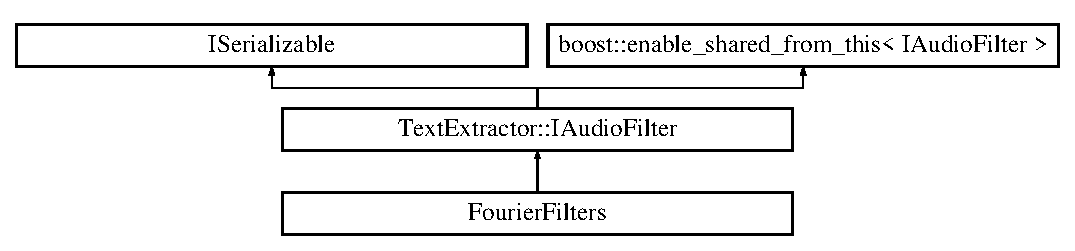
\includegraphics[height=2.926829cm]{class_fourier_filters}
\end{center}
\end{figure}
\subsection*{Classes}
\begin{DoxyCompactItemize}
\item 
class \hyperlink{class_fourier_filters_1_1_i_fourier_filter}{I\+Fourier\+Filter}
\begin{DoxyCompactList}\small\item\em Interface class for any audio filter that operates in the frequency domain. \end{DoxyCompactList}\end{DoxyCompactItemize}
\subsection*{Public Types}
\begin{DoxyCompactItemize}
\item 
\mbox{\Hypertarget{class_fourier_filters_a5ef63b00a3f87418e214e3ca254cb2d7}\label{class_fourier_filters_a5ef63b00a3f87418e214e3ca254cb2d7}} 
typedef std\+::complex$<$ float $>$ \hyperlink{class_fourier_filters_a5ef63b00a3f87418e214e3ca254cb2d7}{Complex\+Num}
\begin{DoxyCompactList}\small\item\em Types. \end{DoxyCompactList}\item 
\mbox{\Hypertarget{class_fourier_filters_a0c1dda206fd4fb5648ef03533562f804}\label{class_fourier_filters_a0c1dda206fd4fb5648ef03533562f804}} 
typedef std\+::valarray$<$ \hyperlink{class_fourier_filters_a5ef63b00a3f87418e214e3ca254cb2d7}{Complex\+Num} $>$ {\bfseries Complex\+Num\+Array}
\end{DoxyCompactItemize}
\subsection*{Public Member Functions}
\begin{DoxyCompactItemize}
\item 
\mbox{\Hypertarget{class_fourier_filters_a1194955fe9d06a2b1453165b5d1375b7}\label{class_fourier_filters_a1194955fe9d06a2b1453165b5d1375b7}} 
{\bfseries R\+T\+T\+I\+\_\+\+D\+E\+CL} ()
\item 
\mbox{\Hypertarget{class_fourier_filters_ab68f377ff94adb8e97c0425f3a7ab711}\label{class_fourier_filters_ab68f377ff94adb8e97c0425f3a7ab711}} 
{\footnotesize template$<$typename T $>$ }\\boost\+::shared\+\_\+ptr$<$ T $>$ {\bfseries Find\+Filter} () const
\item 
\mbox{\Hypertarget{class_fourier_filters_a268c613597b9cf717e1564fe6fa636b9}\label{class_fourier_filters_a268c613597b9cf717e1564fe6fa636b9}} 
\hyperlink{class_fourier_filters_a268c613597b9cf717e1564fe6fa636b9}{Fourier\+Filters} ()
\begin{DoxyCompactList}\small\item\em Construction. \end{DoxyCompactList}\item 
\mbox{\Hypertarget{class_fourier_filters_ae59b98c84e2cae9754bf743b706869d8}\label{class_fourier_filters_ae59b98c84e2cae9754bf743b706869d8}} 
virtual void \hyperlink{class_fourier_filters_ae59b98c84e2cae9754bf743b706869d8}{Serialize} (Json\+::\+Value \&json)
\begin{DoxyCompactList}\small\item\em I\+Serialziable interface. \end{DoxyCompactList}\item 
\mbox{\Hypertarget{class_fourier_filters_a83afe09537b528b8bbc128ce744aaa58}\label{class_fourier_filters_a83afe09537b528b8bbc128ce744aaa58}} 
virtual void {\bfseries Deserialize} (const Json\+::\+Value \&json)
\item 
\mbox{\Hypertarget{class_fourier_filters_ab3c9f0f031eed41cc32f9b2210b88021}\label{class_fourier_filters_ab3c9f0f031eed41cc32f9b2210b88021}} 
virtual void \hyperlink{class_fourier_filters_ab3c9f0f031eed41cc32f9b2210b88021}{Apply\+Filter} (Speech\+Audio\+Data \&a\+\_\+\+Data)
\begin{DoxyCompactList}\small\item\em I\+Audio\+Filter interface. \end{DoxyCompactList}\item 
\mbox{\Hypertarget{class_fourier_filters_a355bfc3ec927b150379cae40896db624}\label{class_fourier_filters_a355bfc3ec927b150379cae40896db624}} 
void \hyperlink{class_fourier_filters_a355bfc3ec927b150379cae40896db624}{Add\+Filter} (\hyperlink{class_fourier_filters_1_1_i_fourier_filter_acad39dd74318f8f8b06d80a00b19f8cb}{I\+Fourier\+Filter\+::\+SP} a\+\_\+\+Filter)
\begin{DoxyCompactList}\small\item\em Mutators. \end{DoxyCompactList}\end{DoxyCompactItemize}
\subsection*{Additional Inherited Members}


The documentation for this class was generated from the following files\+:\begin{DoxyCompactItemize}
\item 
src/extractors/filters/Fourier\+Filters.\+h\item 
src/extractors/filters/Fourier\+Filters.\+cpp\end{DoxyCompactItemize}

\hypertarget{class_gauss_window}{}\section{Gauss\+Window Class Reference}
\label{class_gauss_window}\index{Gauss\+Window@{Gauss\+Window}}
Inheritance diagram for Gauss\+Window\+:\begin{figure}[H]
\begin{center}
\leavevmode
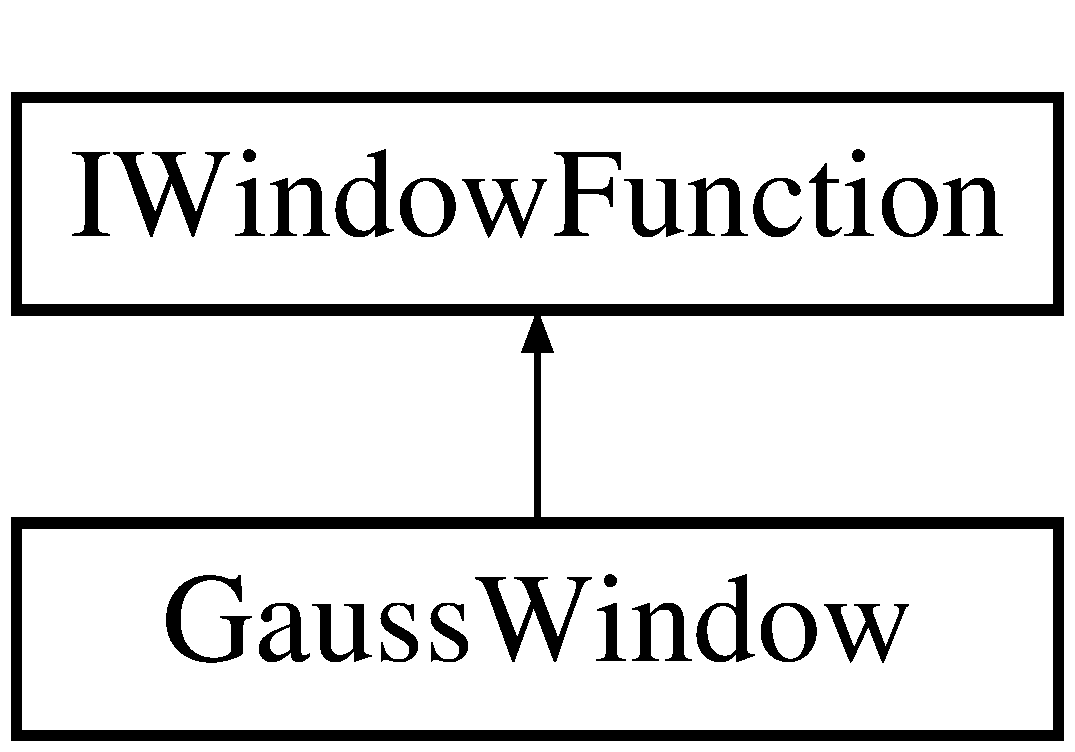
\includegraphics[height=2.000000cm]{class_gauss_window}
\end{center}
\end{figure}
\subsection*{Public Member Functions}
\begin{DoxyCompactItemize}
\item 
\mbox{\Hypertarget{class_gauss_window_a9ac9808a2f043efff93bcd286b6afd61}\label{class_gauss_window_a9ac9808a2f043efff93bcd286b6afd61}} 
{\bfseries Gauss\+Window} (double a\+\_\+\+Alpha=0.\+25)
\item 
\mbox{\Hypertarget{class_gauss_window_acbb50438a57dcc11f351bbd205720ca6}\label{class_gauss_window_acbb50438a57dcc11f351bbd205720ca6}} 
float {\bfseries Value} (int length, int index)
\end{DoxyCompactItemize}
\subsection*{Additional Inherited Members}


The documentation for this class was generated from the following file\+:\begin{DoxyCompactItemize}
\item 
src/utils/fft/Gauss\+Window.\+h\end{DoxyCompactItemize}

\hypertarget{class_gaze_data}{}\section{Gaze\+Data Class Reference}
\label{class_gaze_data}\index{Gaze\+Data@{Gaze\+Data}}
Inheritance diagram for Gaze\+Data\+:\begin{figure}[H]
\begin{center}
\leavevmode
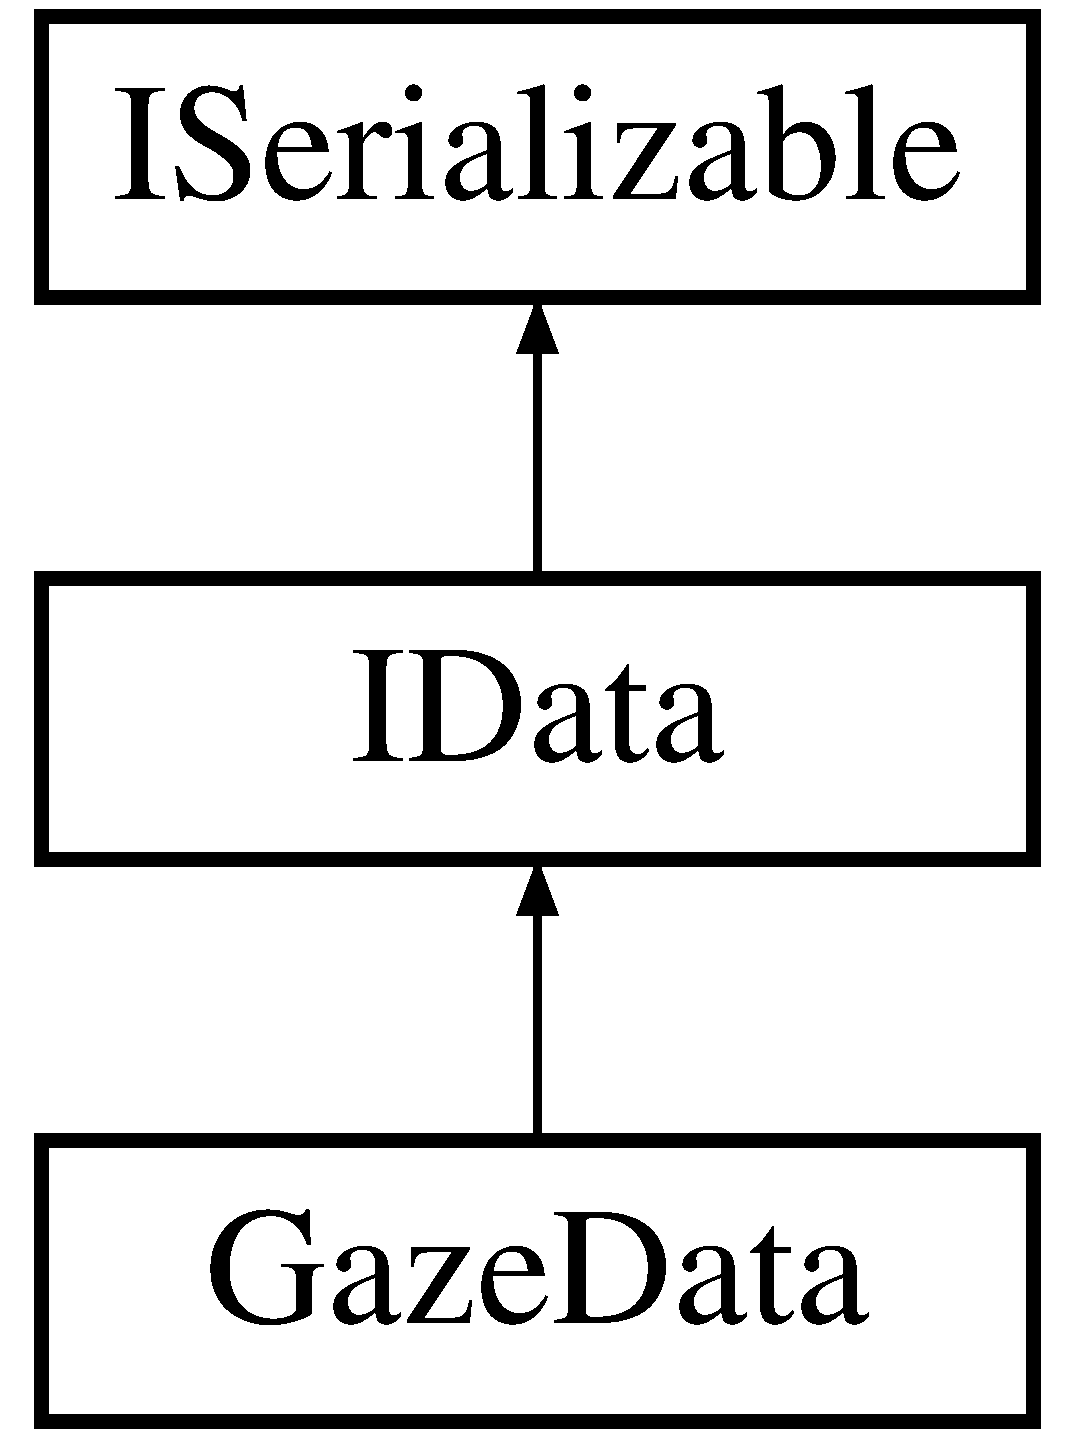
\includegraphics[height=3.000000cm]{class_gaze_data}
\end{center}
\end{figure}
\subsection*{Public Member Functions}
\begin{DoxyCompactItemize}
\item 
\mbox{\Hypertarget{class_gaze_data_ad3928e7241a0d1a5e4503a80a61b9d5c}\label{class_gaze_data_ad3928e7241a0d1a5e4503a80a61b9d5c}} 
{\bfseries R\+T\+T\+I\+\_\+\+D\+E\+CL} ()
\item 
\mbox{\Hypertarget{class_gaze_data_a4cc80b561b9ff9639c6b64dbf90a761b}\label{class_gaze_data_a4cc80b561b9ff9639c6b64dbf90a761b}} 
{\bfseries Gaze\+Data} (bool a\+\_\+\+Is\+Looking=false)
\item 
\mbox{\Hypertarget{class_gaze_data_afb48496a87cd44edc2d0f89a08a1ee8d}\label{class_gaze_data_afb48496a87cd44edc2d0f89a08a1ee8d}} 
virtual void \hyperlink{class_gaze_data_afb48496a87cd44edc2d0f89a08a1ee8d}{Serialize} (Json\+::\+Value \&json)
\begin{DoxyCompactList}\small\item\em I\+Serializable interface. \end{DoxyCompactList}\item 
\mbox{\Hypertarget{class_gaze_data_ab266c4beee8f2df252deb90fc8d737bd}\label{class_gaze_data_ab266c4beee8f2df252deb90fc8d737bd}} 
virtual void {\bfseries Deserialize} (const Json\+::\+Value \&json)
\item 
\mbox{\Hypertarget{class_gaze_data_a97f27e2d25014fd9f6ac694602a60628}\label{class_gaze_data_a97f27e2d25014fd9f6ac694602a60628}} 
bool \hyperlink{class_gaze_data_a97f27e2d25014fd9f6ac694602a60628}{Get\+Is\+Looking} () const
\begin{DoxyCompactList}\small\item\em Accessors. \end{DoxyCompactList}\end{DoxyCompactItemize}


The documentation for this class was generated from the following file\+:\begin{DoxyCompactItemize}
\item 
src/sensors/Gaze\+Data.\+h\end{DoxyCompactItemize}

\hypertarget{class_gesture}{}\section{Gesture Class Reference}
\label{class_gesture}\index{Gesture@{Gesture}}


This object is placed on the blackboard when we need self to say anything.  




{\ttfamily \#include $<$Gesture.\+h$>$}

Inheritance diagram for Gesture\+:\begin{figure}[H]
\begin{center}
\leavevmode
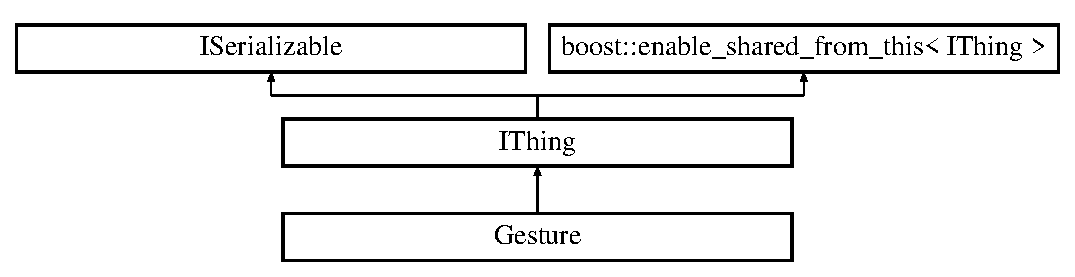
\includegraphics[height=3.000000cm]{class_gesture}
\end{center}
\end{figure}
\subsection*{Public Types}
\begin{DoxyCompactItemize}
\item 
\mbox{\Hypertarget{class_gesture_a33ef75f98bf7b23f861e031e23da0a9f}\label{class_gesture_a33ef75f98bf7b23f861e031e23da0a9f}} 
typedef boost\+::shared\+\_\+ptr$<$ \hyperlink{class_gesture}{Gesture} $>$ \hyperlink{class_gesture_a33ef75f98bf7b23f861e031e23da0a9f}{SP}
\begin{DoxyCompactList}\small\item\em Types. \end{DoxyCompactList}\item 
\mbox{\Hypertarget{class_gesture_aaa739c72bb83c940b5f1bd57f9eb11e8}\label{class_gesture_aaa739c72bb83c940b5f1bd57f9eb11e8}} 
typedef boost\+::weak\+\_\+ptr$<$ \hyperlink{class_gesture}{Gesture} $>$ {\bfseries WP}
\end{DoxyCompactItemize}
\subsection*{Public Member Functions}
\begin{DoxyCompactItemize}
\item 
\mbox{\Hypertarget{class_gesture_ab2d9cebca764207566feffc774dfaa06}\label{class_gesture_ab2d9cebca764207566feffc774dfaa06}} 
{\bfseries R\+T\+T\+I\+\_\+\+D\+E\+CL} ()
\item 
\mbox{\Hypertarget{class_gesture_a7a3df706550bedd9fdd7df76618fd2e6}\label{class_gesture_a7a3df706550bedd9fdd7df76618fd2e6}} 
virtual void \hyperlink{class_gesture_a7a3df706550bedd9fdd7df76618fd2e6}{Serialize} (Json\+::\+Value \&json)
\begin{DoxyCompactList}\small\item\em I\+Serializable interface. \end{DoxyCompactList}\item 
\mbox{\Hypertarget{class_gesture_ae2ffef97bf23de5909bb482d8dc52155}\label{class_gesture_ae2ffef97bf23de5909bb482d8dc52155}} 
virtual void {\bfseries Deserialize} (const Json\+::\+Value \&json)
\item 
\mbox{\Hypertarget{class_gesture_a840ff60bea4128f137c5b114abc844f6}\label{class_gesture_a840ff60bea4128f137c5b114abc844f6}} 
\hyperlink{class_gesture_a840ff60bea4128f137c5b114abc844f6}{Gesture} ()
\begin{DoxyCompactList}\small\item\em Construction. \end{DoxyCompactList}\item 
\mbox{\Hypertarget{class_gesture_ac3c273ee5e5ac8c1a170c97538929aec}\label{class_gesture_ac3c273ee5e5ac8c1a170c97538929aec}} 
{\bfseries Gesture} (const std\+::string \&a\+\_\+\+Type)
\item 
\mbox{\Hypertarget{class_gesture_af0fb78e7c333a92dacef56975eb96e9f}\label{class_gesture_af0fb78e7c333a92dacef56975eb96e9f}} 
{\bfseries Gesture} (const std\+::string \&a\+\_\+\+Type, const \hyperlink{class_params_map}{Params\+Map} \&a\+\_\+\+Params)
\item 
\mbox{\Hypertarget{class_gesture_accb71d86b7be76eb9db494a97122454a}\label{class_gesture_accb71d86b7be76eb9db494a97122454a}} 
const std\+::string \& \hyperlink{class_gesture_accb71d86b7be76eb9db494a97122454a}{Get\+Type} () const
\begin{DoxyCompactList}\small\item\em Accessors. \end{DoxyCompactList}\item 
\mbox{\Hypertarget{class_gesture_a79d4745d74841bbf76ddd094b875ff2d}\label{class_gesture_a79d4745d74841bbf76ddd094b875ff2d}} 
const \hyperlink{class_params_map}{Params\+Map} \& {\bfseries Get\+Params} () const
\item 
\mbox{\Hypertarget{class_gesture_af4c98298c644a7012d9ee45c4c1eb9dd}\label{class_gesture_af4c98298c644a7012d9ee45c4c1eb9dd}} 
void {\bfseries Set\+Type} (const std\+::string \&a\+\_\+\+Type)
\item 
\mbox{\Hypertarget{class_gesture_aba15db55f1cce6ebc0363237b09e0e46}\label{class_gesture_aba15db55f1cce6ebc0363237b09e0e46}} 
void {\bfseries Set\+Params} (const \hyperlink{class_params_map}{Params\+Map} \&a\+\_\+\+Param)
\end{DoxyCompactItemize}
\subsection*{Additional Inherited Members}


\subsection{Detailed Description}
This object is placed on the blackboard when we need self to say anything. 

The documentation for this class was generated from the following files\+:\begin{DoxyCompactItemize}
\item 
src/blackboard/Gesture.\+h\item 
src/blackboard/Gesture.\+cpp\end{DoxyCompactItemize}

\hypertarget{class_gesture_agent}{}\section{Gesture\+Agent Class Reference}
\label{class_gesture_agent}\index{Gesture\+Agent@{Gesture\+Agent}}
Inheritance diagram for Gesture\+Agent\+:\begin{figure}[H]
\begin{center}
\leavevmode
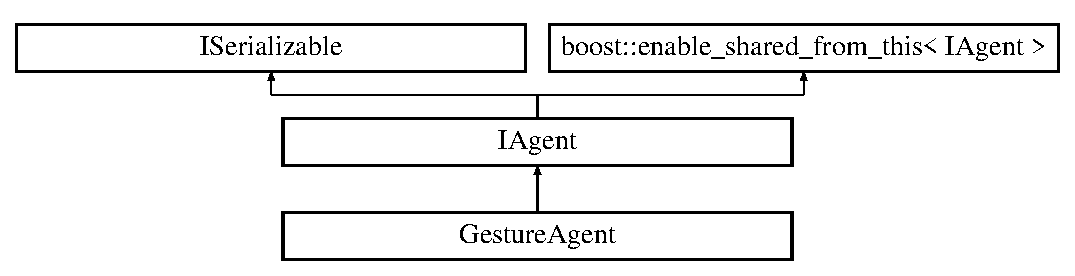
\includegraphics[height=3.000000cm]{class_gesture_agent}
\end{center}
\end{figure}
\subsection*{Public Member Functions}
\begin{DoxyCompactItemize}
\item 
\mbox{\Hypertarget{class_gesture_agent_a78fb03ce29164313330949299bb7cbc9}\label{class_gesture_agent_a78fb03ce29164313330949299bb7cbc9}} 
{\bfseries R\+T\+T\+I\+\_\+\+D\+E\+CL} ()
\item 
\mbox{\Hypertarget{class_gesture_agent_a1dabc7276f42e2574e68b22a6b0a785e}\label{class_gesture_agent_a1dabc7276f42e2574e68b22a6b0a785e}} 
virtual void \hyperlink{class_gesture_agent_a1dabc7276f42e2574e68b22a6b0a785e}{Serialize} (Json\+::\+Value \&json)
\begin{DoxyCompactList}\small\item\em I\+Serializable interface. \end{DoxyCompactList}\item 
\mbox{\Hypertarget{class_gesture_agent_a8d9734b72a1c89e456c10870343abc3c}\label{class_gesture_agent_a8d9734b72a1c89e456c10870343abc3c}} 
virtual void {\bfseries Deserialize} (const Json\+::\+Value \&json)
\item 
\mbox{\Hypertarget{class_gesture_agent_ac773ca370ebf0f93a149d0006f22e498}\label{class_gesture_agent_ac773ca370ebf0f93a149d0006f22e498}} 
virtual bool \hyperlink{class_gesture_agent_ac773ca370ebf0f93a149d0006f22e498}{On\+Start} ()
\begin{DoxyCompactList}\small\item\em \hyperlink{class_i_agent}{I\+Agent} interface. \end{DoxyCompactList}\item 
\mbox{\Hypertarget{class_gesture_agent_aff07bd0cc5e93497f3315bb9119e2403}\label{class_gesture_agent_aff07bd0cc5e93497f3315bb9119e2403}} 
virtual bool {\bfseries On\+Stop} ()
\end{DoxyCompactItemize}
\subsection*{Additional Inherited Members}


The documentation for this class was generated from the following files\+:\begin{DoxyCompactItemize}
\item 
src/agent/Gesture\+Agent.\+h\item 
src/agent/Gesture\+Agent.\+cpp\end{DoxyCompactItemize}

\hypertarget{class_gesture_data}{}\section{Gesture\+Data Class Reference}
\label{class_gesture_data}\index{Gesture\+Data@{Gesture\+Data}}
Inheritance diagram for Gesture\+Data\+:\begin{figure}[H]
\begin{center}
\leavevmode
\includegraphics[height=3.000000cm]{class_gesture_data}
\end{center}
\end{figure}
\subsection*{Public Member Functions}
\begin{DoxyCompactItemize}
\item 
\mbox{\Hypertarget{class_gesture_data_af621636ce91a725ddfde0a0a8b2c45fc}\label{class_gesture_data_af621636ce91a725ddfde0a0a8b2c45fc}} 
{\bfseries R\+T\+T\+I\+\_\+\+D\+E\+CL} ()
\item 
\mbox{\Hypertarget{class_gesture_data_aaeb8ce0d155e61d524cce6627b12e120}\label{class_gesture_data_aaeb8ce0d155e61d524cce6627b12e120}} 
{\bfseries Gesture\+Data} (const std\+::string \&a\+\_\+\+Gesture)
\item 
\mbox{\Hypertarget{class_gesture_data_ae443ed652dc782ce640bf8c1bee92e05}\label{class_gesture_data_ae443ed652dc782ce640bf8c1bee92e05}} 
virtual void \hyperlink{class_gesture_data_ae443ed652dc782ce640bf8c1bee92e05}{Serialize} (Json\+::\+Value \&json)
\begin{DoxyCompactList}\small\item\em I\+Serializable interface. \end{DoxyCompactList}\item 
\mbox{\Hypertarget{class_gesture_data_aa43ed19ab947af9807dbb5f5027bb006}\label{class_gesture_data_aa43ed19ab947af9807dbb5f5027bb006}} 
virtual void {\bfseries Deserialize} (const Json\+::\+Value \&json)
\item 
\mbox{\Hypertarget{class_gesture_data_ab4981395f482b77e42f77f76912ce5e0}\label{class_gesture_data_ab4981395f482b77e42f77f76912ce5e0}} 
const std\+::string \& \hyperlink{class_gesture_data_ab4981395f482b77e42f77f76912ce5e0}{Get\+Gesture} () const
\begin{DoxyCompactList}\small\item\em Accessors. \end{DoxyCompactList}\item 
\mbox{\Hypertarget{class_gesture_data_affdb41d37986bd7125d23c3020a5ee36}\label{class_gesture_data_affdb41d37986bd7125d23c3020a5ee36}} 
void {\bfseries Set\+Gesture} (const std\+::string \&a\+\_\+\+Gesture)
\end{DoxyCompactItemize}


The documentation for this class was generated from the following file\+:\begin{DoxyCompactItemize}
\item 
src/sensors/Gesture\+Data.\+h\end{DoxyCompactItemize}

\hypertarget{class_gesture_extractor}{}\section{Gesture\+Extractor Class Reference}
\label{class_gesture_extractor}\index{Gesture\+Extractor@{Gesture\+Extractor}}
Inheritance diagram for Gesture\+Extractor\+:\begin{figure}[H]
\begin{center}
\leavevmode
\includegraphics[height=2.625000cm]{class_gesture_extractor}
\end{center}
\end{figure}
\subsection*{Public Member Functions}
\begin{DoxyCompactItemize}
\item 
\mbox{\Hypertarget{class_gesture_extractor_a9f1f7f89ddb994175e5118d25e8362c7}\label{class_gesture_extractor_a9f1f7f89ddb994175e5118d25e8362c7}} 
{\bfseries R\+T\+T\+I\+\_\+\+D\+E\+CL} ()
\item 
\mbox{\Hypertarget{class_gesture_extractor_a9ef26ad3dd52fd891884cfb91b799577}\label{class_gesture_extractor_a9ef26ad3dd52fd891884cfb91b799577}} 
virtual const char $\ast$ \hyperlink{class_gesture_extractor_a9ef26ad3dd52fd891884cfb91b799577}{Get\+Name} () const
\begin{DoxyCompactList}\small\item\em \hyperlink{class_i_feature_extractor}{I\+Feature\+Extractor} interface. \end{DoxyCompactList}\item 
\mbox{\Hypertarget{class_gesture_extractor_a21246649d97810dbe17607e3e57fa425}\label{class_gesture_extractor_a21246649d97810dbe17607e3e57fa425}} 
virtual bool {\bfseries On\+Start} ()
\item 
\mbox{\Hypertarget{class_gesture_extractor_af4b63402b7b7e93600650b62638dfb0b}\label{class_gesture_extractor_af4b63402b7b7e93600650b62638dfb0b}} 
virtual bool {\bfseries On\+Stop} ()
\end{DoxyCompactItemize}
\subsection*{Additional Inherited Members}


The documentation for this class was generated from the following files\+:\begin{DoxyCompactItemize}
\item 
src/extractors/Gesture\+Extractor.\+h\item 
src/extractors/Gesture\+Extractor.\+cpp\end{DoxyCompactItemize}

\hypertarget{class_gesture_manager}{}\section{Gesture\+Manager Class Reference}
\label{class_gesture_manager}\index{Gesture\+Manager@{Gesture\+Manager}}


{\ttfamily \#include $<$Gesture\+Manager.\+h$>$}

Inheritance diagram for Gesture\+Manager\+:\begin{figure}[H]
\begin{center}
\leavevmode
\includegraphics[height=2.000000cm]{class_gesture_manager}
\end{center}
\end{figure}
\subsection*{Public Types}
\begin{DoxyCompactItemize}
\item 
\mbox{\Hypertarget{class_gesture_manager_a72da7b5c9399cc34be1ec0337c447f54}\label{class_gesture_manager_a72da7b5c9399cc34be1ec0337c447f54}} 
typedef std\+::list$<$ std\+::string $>$ \hyperlink{class_gesture_manager_a72da7b5c9399cc34be1ec0337c447f54}{Gesture\+Files}
\begin{DoxyCompactList}\small\item\em Types. \end{DoxyCompactList}\item 
\mbox{\Hypertarget{class_gesture_manager_adf20e982b5dfe2f8cd9ef357211d4a2d}\label{class_gesture_manager_adf20e982b5dfe2f8cd9ef357211d4a2d}} 
typedef boost\+::shared\+\_\+ptr$<$ \hyperlink{class_i_gesture}{I\+Gesture} $>$ {\bfseries I\+Gesture\+SP}
\item 
\mbox{\Hypertarget{class_gesture_manager_a51038e010deb91bf4df120bf34e7eee2}\label{class_gesture_manager_a51038e010deb91bf4df120bf34e7eee2}} 
typedef boost\+::shared\+\_\+ptr$<$ \hyperlink{class_proxy_gesture}{Proxy\+Gesture} $>$ {\bfseries Proxy\+Gesture\+SP}
\item 
\mbox{\Hypertarget{class_gesture_manager_a572b1d9a614d6ed3642618efa3fc8c4c}\label{class_gesture_manager_a572b1d9a614d6ed3642618efa3fc8c4c}} 
typedef std\+::vector$<$ I\+Gesture\+SP $>$ {\bfseries Gesture\+List}
\item 
\mbox{\Hypertarget{class_gesture_manager_ad61019472923fab10fc3333e70cc19e4}\label{class_gesture_manager_ad61019472923fab10fc3333e70cc19e4}} 
typedef std\+::multimap$<$ std\+::string, I\+Gesture\+SP $>$ {\bfseries Gesture\+Map}
\item 
\mbox{\Hypertarget{class_gesture_manager_a9cdebb5ea97129019db72056043792c7}\label{class_gesture_manager_a9cdebb5ea97129019db72056043792c7}} 
typedef std\+::map$<$ std\+::string, Proxy\+Gesture\+SP $>$ {\bfseries Proxy\+Map}
\item 
\mbox{\Hypertarget{class_gesture_manager_af19a0f40db6d9f52ce6f52e029f137e3}\label{class_gesture_manager_af19a0f40db6d9f52ce6f52e029f137e3}} 
typedef Factory$<$ \hyperlink{class_i_gesture}{I\+Gesture} $>$ {\bfseries Gesture\+Factory}
\item 
\mbox{\Hypertarget{class_gesture_manager_a949853cf7837f7f20da2aa66ef769766}\label{class_gesture_manager_a949853cf7837f7f20da2aa66ef769766}} 
typedef Delegate$<$ \hyperlink{class_i_gesture}{I\+Gesture} $\ast$ $>$ {\bfseries Gesture\+Delegate}
\end{DoxyCompactItemize}
\subsection*{Public Member Functions}
\begin{DoxyCompactItemize}
\item 
\mbox{\Hypertarget{class_gesture_manager_a568a60a3f0763d9d26991a6da3abd8b9}\label{class_gesture_manager_a568a60a3f0763d9d26991a6da3abd8b9}} 
{\bfseries R\+T\+T\+I\+\_\+\+D\+E\+CL} ()
\item 
\mbox{\Hypertarget{class_gesture_manager_a5ecfa8bb990c8b2064df5051848845a1}\label{class_gesture_manager_a5ecfa8bb990c8b2064df5051848845a1}} 
\hyperlink{class_gesture_manager_a5ecfa8bb990c8b2064df5051848845a1}{Gesture\+Manager} ()
\begin{DoxyCompactList}\small\item\em Construction. \end{DoxyCompactList}\item 
\mbox{\Hypertarget{class_gesture_manager_ad785801d982e5a8f1b943fe8d042ba27}\label{class_gesture_manager_ad785801d982e5a8f1b943fe8d042ba27}} 
virtual void \hyperlink{class_gesture_manager_ad785801d982e5a8f1b943fe8d042ba27}{Serialize} (Json\+::\+Value \&json)
\begin{DoxyCompactList}\small\item\em I\+Serializable interface. \end{DoxyCompactList}\item 
\mbox{\Hypertarget{class_gesture_manager_afafe002820cead44bead7c4dea9a16f7}\label{class_gesture_manager_afafe002820cead44bead7c4dea9a16f7}} 
virtual void {\bfseries Deserialize} (const Json\+::\+Value \&json)
\item 
\mbox{\Hypertarget{class_gesture_manager_a12fa31aabe615a3190e8eda374a11558}\label{class_gesture_manager_a12fa31aabe615a3190e8eda374a11558}} 
const Gesture\+Map \& \hyperlink{class_gesture_manager_a12fa31aabe615a3190e8eda374a11558}{Get\+Gesture\+Map} () const
\begin{DoxyCompactList}\small\item\em Accessors. \end{DoxyCompactList}\item 
\mbox{\Hypertarget{class_gesture_manager_af3d61e28375c7e0a38b4c4fa43138f7a}\label{class_gesture_manager_af3d61e28375c7e0a38b4c4fa43138f7a}} 
bool \hyperlink{class_gesture_manager_af3d61e28375c7e0a38b4c4fa43138f7a}{Find\+Gestures} (const std\+::string \&a\+\_\+\+Gesture\+Id, Gesture\+List \&a\+\_\+\+Gestures) const
\begin{DoxyCompactList}\small\item\em This finds all gestures who have the given ID, returns false if none are found. \end{DoxyCompactList}\item 
\mbox{\Hypertarget{class_gesture_manager_ab227e6b7b7e111594725fcd3e571e929}\label{class_gesture_manager_ab227e6b7b7e111594725fcd3e571e929}} 
bool \hyperlink{class_gesture_manager_ab227e6b7b7e111594725fcd3e571e929}{Start} (const \hyperlink{class_gesture_manager_a72da7b5c9399cc34be1ec0337c447f54}{Gesture\+Files} \&a\+\_\+\+Files)
\begin{DoxyCompactList}\small\item\em Initialize and start this sensor manager. \end{DoxyCompactList}\item 
\mbox{\Hypertarget{class_gesture_manager_a22472656b5488240160d5a9bde47aa6a}\label{class_gesture_manager_a22472656b5488240160d5a9bde47aa6a}} 
bool \hyperlink{class_gesture_manager_a22472656b5488240160d5a9bde47aa6a}{Stop} ()
\begin{DoxyCompactList}\small\item\em Stop this sensor manager. \end{DoxyCompactList}\item 
\mbox{\Hypertarget{class_gesture_manager_a861ab88404e3de59931aea922c6b5f87}\label{class_gesture_manager_a861ab88404e3de59931aea922c6b5f87}} 
bool {\bfseries Add\+Gesture} (const I\+Gesture\+SP \&a\+\_\+sp\+Gesture)
\item 
\mbox{\Hypertarget{class_gesture_manager_afd960ebe3b54c2d61ea40676743b2f84}\label{class_gesture_manager_afd960ebe3b54c2d61ea40676743b2f84}} 
bool {\bfseries Remove\+Gesture} (const I\+Gesture\+SP \&a\+\_\+sp\+Gesture)
\end{DoxyCompactItemize}


\subsection{Detailed Description}
This manager manages all gestures available to the local self instance. Normally a Skill\+Gesture will invoke into this manager to execute various gestures to perform actions. 

The documentation for this class was generated from the following files\+:\begin{DoxyCompactItemize}
\item 
src/gestures/Gesture\+Manager.\+h\item 
src/gestures/Gesture\+Manager.\+cpp\end{DoxyCompactItemize}

\hypertarget{class_gesture_sensor}{}\section{Gesture\+Sensor Class Reference}
\label{class_gesture_sensor}\index{Gesture\+Sensor@{Gesture\+Sensor}}


Base class for a \hyperlink{class_gesture}{Gesture} Sensor class.  




{\ttfamily \#include $<$Gesture\+Sensor.\+h$>$}

Inheritance diagram for Gesture\+Sensor\+:\begin{figure}[H]
\begin{center}
\leavevmode
\includegraphics[height=3.000000cm]{class_gesture_sensor}
\end{center}
\end{figure}
\subsection*{Public Member Functions}
\begin{DoxyCompactItemize}
\item 
\mbox{\Hypertarget{class_gesture_sensor_a2262485356c60a9d0bf5e6ffdcbe3a4c}\label{class_gesture_sensor_a2262485356c60a9d0bf5e6ffdcbe3a4c}} 
{\bfseries R\+T\+T\+I\+\_\+\+D\+E\+CL} ()
\item 
\mbox{\Hypertarget{class_gesture_sensor_ae69a58945c1572e0aac47a75a0fe4b7e}\label{class_gesture_sensor_ae69a58945c1572e0aac47a75a0fe4b7e}} 
virtual void \hyperlink{class_gesture_sensor_ae69a58945c1572e0aac47a75a0fe4b7e}{Serialize} (Json\+::\+Value \&json)
\begin{DoxyCompactList}\small\item\em I\+Serialiazable interface. \end{DoxyCompactList}\item 
\mbox{\Hypertarget{class_gesture_sensor_a6e07179b4b799de3dea6234cde01ab3e}\label{class_gesture_sensor_a6e07179b4b799de3dea6234cde01ab3e}} 
virtual void {\bfseries Deserialize} (const Json\+::\+Value \&json)
\item 
\mbox{\Hypertarget{class_gesture_sensor_ae62b4d22b9e8a116e92190d2d8dfe2ea}\label{class_gesture_sensor_ae62b4d22b9e8a116e92190d2d8dfe2ea}} 
virtual const char $\ast$ \hyperlink{class_gesture_sensor_ae62b4d22b9e8a116e92190d2d8dfe2ea}{Get\+Sensor\+Name} ()
\begin{DoxyCompactList}\small\item\em \hyperlink{class_i_sensor}{I\+Sensor} interface. \end{DoxyCompactList}\item 
\mbox{\Hypertarget{class_gesture_sensor_a77ec8b522049505ce9f5072a59bf1c62}\label{class_gesture_sensor_a77ec8b522049505ce9f5072a59bf1c62}} 
virtual const char $\ast$ {\bfseries Get\+Data\+Type} ()
\item 
\mbox{\Hypertarget{class_gesture_sensor_a4743a42260f8aeb0b71ef6d85eb3b343}\label{class_gesture_sensor_a4743a42260f8aeb0b71ef6d85eb3b343}} 
virtual bool \hyperlink{class_gesture_sensor_a4743a42260f8aeb0b71ef6d85eb3b343}{On\+Start} ()
\begin{DoxyCompactList}\small\item\em This is invoked when the first subscriber subscribes to this sensor. \end{DoxyCompactList}\item 
\mbox{\Hypertarget{class_gesture_sensor_ab7db8e69526a7e98d3feb8889759b2ca}\label{class_gesture_sensor_ab7db8e69526a7e98d3feb8889759b2ca}} 
virtual bool \hyperlink{class_gesture_sensor_ab7db8e69526a7e98d3feb8889759b2ca}{On\+Stop} ()
\begin{DoxyCompactList}\small\item\em This is invoked when the last subscriber un-\/subscribes. \end{DoxyCompactList}\item 
\mbox{\Hypertarget{class_gesture_sensor_adda207e7d5e86f79dbbfceede21f7c91}\label{class_gesture_sensor_adda207e7d5e86f79dbbfceede21f7c91}} 
virtual void \hyperlink{class_gesture_sensor_adda207e7d5e86f79dbbfceede21f7c91}{On\+Pause} ()
\begin{DoxyCompactList}\small\item\em This is invoked to pause this sensor. \end{DoxyCompactList}\item 
\mbox{\Hypertarget{class_gesture_sensor_af9ebfec9b18d1eab71d06f8f0f62e9ed}\label{class_gesture_sensor_af9ebfec9b18d1eab71d06f8f0f62e9ed}} 
virtual void \hyperlink{class_gesture_sensor_af9ebfec9b18d1eab71d06f8f0f62e9ed}{On\+Resume} ()
\begin{DoxyCompactList}\small\item\em This is invoked to restart this sensor. \end{DoxyCompactList}\end{DoxyCompactItemize}
\subsection*{Additional Inherited Members}


\subsection{Detailed Description}
Base class for a \hyperlink{class_gesture}{Gesture} Sensor class. 

The documentation for this class was generated from the following files\+:\begin{DoxyCompactItemize}
\item 
src/sensors/Gesture\+Sensor.\+h\item 
src/sensors/Gesture\+Sensor.\+cpp\end{DoxyCompactItemize}

\hypertarget{class_gesture_skill}{}\section{Gesture\+Skill Class Reference}
\label{class_gesture_skill}\index{Gesture\+Skill@{Gesture\+Skill}}


This skill executes a gestures in the gesture manager.  




{\ttfamily \#include $<$Gesture\+Skill.\+h$>$}

Inheritance diagram for Gesture\+Skill\+:\begin{figure}[H]
\begin{center}
\leavevmode
\includegraphics[height=3.000000cm]{class_gesture_skill}
\end{center}
\end{figure}
\subsection*{Public Types}
\begin{DoxyCompactItemize}
\item 
\mbox{\Hypertarget{class_gesture_skill_ab8669ee642c7c699bcabf333852fbb74}\label{class_gesture_skill_ab8669ee642c7c699bcabf333852fbb74}} 
typedef std\+::list$<$ \hyperlink{class_i_skill}{I\+Skill} $\ast$$>$ \hyperlink{class_gesture_skill_ab8669ee642c7c699bcabf333852fbb74}{Skill\+List}
\begin{DoxyCompactList}\small\item\em Types. \end{DoxyCompactList}\end{DoxyCompactItemize}
\subsection*{Public Member Functions}
\begin{DoxyCompactItemize}
\item 
\mbox{\Hypertarget{class_gesture_skill_af813f9000835a90a5f913a68224eafb7}\label{class_gesture_skill_af813f9000835a90a5f913a68224eafb7}} 
{\bfseries R\+T\+T\+I\+\_\+\+D\+E\+CL} ()
\item 
\mbox{\Hypertarget{class_gesture_skill_a3ed1fb78c858d9f70ac8b0e894c345d4}\label{class_gesture_skill_a3ed1fb78c858d9f70ac8b0e894c345d4}} 
\hyperlink{class_gesture_skill_a3ed1fb78c858d9f70ac8b0e894c345d4}{Gesture\+Skill} ()
\begin{DoxyCompactList}\small\item\em Construction. \end{DoxyCompactList}\item 
\mbox{\Hypertarget{class_gesture_skill_ae47ed58380ac3ba82edc622ffc20e053}\label{class_gesture_skill_ae47ed58380ac3ba82edc622ffc20e053}} 
{\bfseries Gesture\+Skill} (const \hyperlink{class_gesture_skill}{Gesture\+Skill} \&a\+\_\+\+Copy)
\item 
\mbox{\Hypertarget{class_gesture_skill_a54bcd1b0b3901d98aaae29262decae25}\label{class_gesture_skill_a54bcd1b0b3901d98aaae29262decae25}} 
{\bfseries Gesture\+Skill} (const std\+::string \&a\+\_\+\+Gesture\+ID)
\item 
\mbox{\Hypertarget{class_gesture_skill_ae5e37990e118acf550a1091fb96efb1e}\label{class_gesture_skill_ae5e37990e118acf550a1091fb96efb1e}} 
const std\+::string \& {\bfseries Get\+Gesture\+Id} () const
\item 
\mbox{\Hypertarget{class_gesture_skill_a0b60ccdba1e8bacc76d135a021b08839}\label{class_gesture_skill_a0b60ccdba1e8bacc76d135a021b08839}} 
const \hyperlink{class_params_map}{Params\+Map} \& {\bfseries Get\+Gesture\+Params} () const
\item 
\mbox{\Hypertarget{class_gesture_skill_aef9c81c6b8c4cd3d6907319f6abfb056}\label{class_gesture_skill_aef9c81c6b8c4cd3d6907319f6abfb056}} 
void {\bfseries Set\+Gesture\+Id} (const std\+::string \&a\+\_\+\+Gesture\+Id)
\item 
\mbox{\Hypertarget{class_gesture_skill_a18c845d82e55043b612e1a52e8cd5bfb}\label{class_gesture_skill_a18c845d82e55043b612e1a52e8cd5bfb}} 
void {\bfseries Set\+Gesture\+Params} (const \hyperlink{class_params_map}{Params\+Map} \&a\+\_\+\+Params)
\item 
\mbox{\Hypertarget{class_gesture_skill_a9a0b5dcba0cbbced2bfc5108304d7513}\label{class_gesture_skill_a9a0b5dcba0cbbced2bfc5108304d7513}} 
virtual void \hyperlink{class_gesture_skill_a9a0b5dcba0cbbced2bfc5108304d7513}{Serialize} (Json\+::\+Value \&json)
\begin{DoxyCompactList}\small\item\em I\+Serializable interface. \end{DoxyCompactList}\item 
\mbox{\Hypertarget{class_gesture_skill_a16b99eb71c3757981012b70979cd5b85}\label{class_gesture_skill_a16b99eb71c3757981012b70979cd5b85}} 
virtual void {\bfseries Deserialize} (const Json\+::\+Value \&json)
\item 
\mbox{\Hypertarget{class_gesture_skill_a44a7d102f239e72a1199c122f33d19ba}\label{class_gesture_skill_a44a7d102f239e72a1199c122f33d19ba}} 
virtual bool \hyperlink{class_gesture_skill_a44a7d102f239e72a1199c122f33d19ba}{Can\+Use\+Skill} ()
\begin{DoxyCompactList}\small\item\em \hyperlink{class_i_skill}{I\+Skill} interface. \end{DoxyCompactList}\item 
\mbox{\Hypertarget{class_gesture_skill_a2cecea782e270b8e7fe86189f839c1e7}\label{class_gesture_skill_a2cecea782e270b8e7fe86189f839c1e7}} 
virtual void \hyperlink{class_gesture_skill_a2cecea782e270b8e7fe86189f839c1e7}{Use\+Skill} (Delegate$<$ \hyperlink{class_i_skill}{I\+Skill} $\ast$$>$ a\+\_\+\+Callback, const \hyperlink{class_params_map}{Params\+Map} \&a\+\_\+\+Params)
\begin{DoxyCompactList}\small\item\em This should return true if this skill can be used, false is returned otherwise. \end{DoxyCompactList}\item 
\mbox{\Hypertarget{class_gesture_skill_a20d5b15e86591d642c89c492bf29b66e}\label{class_gesture_skill_a20d5b15e86591d642c89c492bf29b66e}} 
virtual bool {\bfseries Abort\+Skill} ()
\item 
\mbox{\Hypertarget{class_gesture_skill_ac903e6f48157179e362f680e99274dcc}\label{class_gesture_skill_ac903e6f48157179e362f680e99274dcc}} 
virtual \hyperlink{class_i_skill}{I\+Skill} $\ast$ \hyperlink{class_gesture_skill_ac903e6f48157179e362f680e99274dcc}{Clone} ()
\begin{DoxyCompactList}\small\item\em Invoke this function to stop using this skill, the callback passed to \hyperlink{class_gesture_skill_a2cecea782e270b8e7fe86189f839c1e7}{Use\+Skill()} will N\+OT be invoked after this is called. \end{DoxyCompactList}\end{DoxyCompactItemize}
\subsection*{Additional Inherited Members}


\subsection{Detailed Description}
This skill executes a gestures in the gesture manager. 

The documentation for this class was generated from the following files\+:\begin{DoxyCompactItemize}
\item 
src/skills/Gesture\+Skill.\+h\item 
src/skills/Gesture\+Skill.\+cpp\end{DoxyCompactItemize}

\hypertarget{class_goal}{}\section{Goal Class Reference}
\label{class_goal}\index{Goal@{Goal}}


{\ttfamily \#include $<$Goal.\+h$>$}

Inheritance diagram for Goal\+:\begin{figure}[H]
\begin{center}
\leavevmode
\includegraphics[height=3.000000cm]{class_goal}
\end{center}
\end{figure}
\subsection*{Public Types}
\begin{DoxyCompactItemize}
\item 
\mbox{\Hypertarget{class_goal_a818ae12a4d1f28bd433dab2a830a390e}\label{class_goal_a818ae12a4d1f28bd433dab2a830a390e}} 
typedef boost\+::shared\+\_\+ptr$<$ \hyperlink{class_goal}{Goal} $>$ \hyperlink{class_goal_a818ae12a4d1f28bd433dab2a830a390e}{SP}
\begin{DoxyCompactList}\small\item\em Types. \end{DoxyCompactList}\item 
\mbox{\Hypertarget{class_goal_a2ed42e0bd1adf651fc2514b58af7ea4d}\label{class_goal_a2ed42e0bd1adf651fc2514b58af7ea4d}} 
typedef boost\+::weak\+\_\+ptr$<$ \hyperlink{class_goal}{Goal} $>$ {\bfseries WP}
\end{DoxyCompactItemize}
\subsection*{Public Member Functions}
\begin{DoxyCompactItemize}
\item 
\mbox{\Hypertarget{class_goal_a7d79f22200beca322bcd7d233377169c}\label{class_goal_a7d79f22200beca322bcd7d233377169c}} 
{\bfseries R\+T\+T\+I\+\_\+\+D\+E\+CL} ()
\item 
\mbox{\Hypertarget{class_goal_aef5013c9bf548e51178f58da869d508a}\label{class_goal_aef5013c9bf548e51178f58da869d508a}} 
\hyperlink{class_goal_aef5013c9bf548e51178f58da869d508a}{Goal} ()
\begin{DoxyCompactList}\small\item\em Construction. \end{DoxyCompactList}\item 
\mbox{\Hypertarget{class_goal_a30de5f1c4006f0158cba622816652c07}\label{class_goal_a30de5f1c4006f0158cba622816652c07}} 
{\bfseries Goal} (const std\+::string \&a\+\_\+\+Name)
\item 
\mbox{\Hypertarget{class_goal_a75f87281e05255c70796ea73a17a9ef5}\label{class_goal_a75f87281e05255c70796ea73a17a9ef5}} 
{\bfseries Goal} (const std\+::string \&a\+\_\+\+Name, const \hyperlink{class_params_map}{Params\+Map} \&a\+\_\+\+Params)
\item 
\mbox{\Hypertarget{class_goal_a2096d4ea4b752a795a96f50ebb699a16}\label{class_goal_a2096d4ea4b752a795a96f50ebb699a16}} 
virtual void \hyperlink{class_goal_a2096d4ea4b752a795a96f50ebb699a16}{Serialize} (Json\+::\+Value \&json)
\begin{DoxyCompactList}\small\item\em I\+Serializable interface. \end{DoxyCompactList}\item 
\mbox{\Hypertarget{class_goal_a813bc3e77a58fcbbc2516ea392e3b49e}\label{class_goal_a813bc3e77a58fcbbc2516ea392e3b49e}} 
virtual void {\bfseries Deserialize} (const Json\+::\+Value \&json)
\item 
\mbox{\Hypertarget{class_goal_a64b7107f65dcc2342abf96fbfbe4840e}\label{class_goal_a64b7107f65dcc2342abf96fbfbe4840e}} 
const std\+::string \& \hyperlink{class_goal_a64b7107f65dcc2342abf96fbfbe4840e}{Get\+Name} () const
\begin{DoxyCompactList}\small\item\em Accessors. \end{DoxyCompactList}\item 
\mbox{\Hypertarget{class_goal_aa4f2805affa84db1dd3e7b0e2806fecc}\label{class_goal_aa4f2805affa84db1dd3e7b0e2806fecc}} 
const \hyperlink{class_params_map}{Params\+Map} \& {\bfseries Get\+Params} () const
\item 
\mbox{\Hypertarget{class_goal_aa12d8e975f52616e9f51fe7c1a4151ab}\label{class_goal_aa12d8e975f52616e9f51fe7c1a4151ab}} 
\hyperlink{class_params_map}{Params\+Map} \& {\bfseries Get\+Params} ()
\item 
\mbox{\Hypertarget{class_goal_ab9ef63d5c7740d055a878897a3d75851}\label{class_goal_ab9ef63d5c7740d055a878897a3d75851}} 
void \hyperlink{class_goal_ab9ef63d5c7740d055a878897a3d75851}{Set\+Name} (const std\+::string \&a\+\_\+\+Name)
\begin{DoxyCompactList}\small\item\em Mutators. \end{DoxyCompactList}\item 
\mbox{\Hypertarget{class_goal_a570e141b2be345955ca13e674abed787}\label{class_goal_a570e141b2be345955ca13e674abed787}} 
void {\bfseries Set\+Params} (const \hyperlink{class_params_map}{Params\+Map} \&a\+\_\+\+Params)
\end{DoxyCompactItemize}
\subsection*{Additional Inherited Members}


\subsection{Detailed Description}
This object represents a goal that is added by a agent onto the Blackboard. Once a goal is added the Goal\+Manager will pass the goal onto the \hyperlink{class_plan_manager}{Plan\+Manager} and track a \hyperlink{class_plan_instance}{Plan\+Instance} object until the goal is completed or failed. 

The documentation for this class was generated from the following files\+:\begin{DoxyCompactItemize}
\item 
src/blackboard/Goal.\+h\item 
src/blackboard/Goal.\+cpp\end{DoxyCompactItemize}

\hypertarget{class_goal_agent}{}\section{Goal\+Agent Class Reference}
\label{class_goal_agent}\index{Goal\+Agent@{Goal\+Agent}}


{\ttfamily \#include $<$Goal\+Agent.\+h$>$}

Inheritance diagram for Goal\+Agent\+:\begin{figure}[H]
\begin{center}
\leavevmode
\includegraphics[height=3.000000cm]{class_goal_agent}
\end{center}
\end{figure}
\subsection*{Public Member Functions}
\begin{DoxyCompactItemize}
\item 
\mbox{\Hypertarget{class_goal_agent_a60bcb89ec117fb470a9c34b36fcbca0d}\label{class_goal_agent_a60bcb89ec117fb470a9c34b36fcbca0d}} 
{\bfseries R\+T\+T\+I\+\_\+\+D\+E\+CL} ()
\item 
\mbox{\Hypertarget{class_goal_agent_a750c0d6e115e0465a93ff0432149aafa}\label{class_goal_agent_a750c0d6e115e0465a93ff0432149aafa}} 
\hyperlink{class_goal_agent_a750c0d6e115e0465a93ff0432149aafa}{Goal\+Agent} ()
\begin{DoxyCompactList}\small\item\em Construction. \end{DoxyCompactList}\item 
\mbox{\Hypertarget{class_goal_agent_a0da566247d12224944419be690310a1c}\label{class_goal_agent_a0da566247d12224944419be690310a1c}} 
const char $\ast$ \hyperlink{class_goal_agent_a0da566247d12224944419be690310a1c}{Get\+Name} () const
\begin{DoxyCompactList}\small\item\em \hyperlink{class_i_agent}{I\+Agent} interface. \end{DoxyCompactList}\item 
\mbox{\Hypertarget{class_goal_agent_a5036cfe447ac9867e813bce49c77cf71}\label{class_goal_agent_a5036cfe447ac9867e813bce49c77cf71}} 
bool \hyperlink{class_goal_agent_a5036cfe447ac9867e813bce49c77cf71}{On\+Start} ()
\begin{DoxyCompactList}\small\item\em Interface. \end{DoxyCompactList}\item 
\mbox{\Hypertarget{class_goal_agent_ad3d76e7667e01b1a846f44e7512b40e4}\label{class_goal_agent_ad3d76e7667e01b1a846f44e7512b40e4}} 
bool {\bfseries On\+Stop} ()
\end{DoxyCompactItemize}
\subsection*{Additional Inherited Members}


\subsection{Detailed Description}
This goal manager watches for goals on the blackboard, and creates the plans for those goals. It tracks those plans and updates the goals as the plan state changes. 

The documentation for this class was generated from the following files\+:\begin{DoxyCompactItemize}
\item 
src/agent/Goal\+Agent.\+h\item 
src/agent/Goal\+Agent.\+cpp\end{DoxyCompactItemize}

\hypertarget{struct_goal_name_condition}{}\section{Goal\+Name\+Condition Struct Reference}
\label{struct_goal_name_condition}\index{Goal\+Name\+Condition@{Goal\+Name\+Condition}}


This condition tests against the name of the \hyperlink{class_goal}{Goal} object.  




{\ttfamily \#include $<$Goal\+Name\+Condition.\+h$>$}

Inheritance diagram for Goal\+Name\+Condition\+:\begin{figure}[H]
\begin{center}
\leavevmode
\includegraphics[height=2.014389cm]{struct_goal_name_condition}
\end{center}
\end{figure}
\subsection*{Public Member Functions}
\begin{DoxyCompactItemize}
\item 
\mbox{\Hypertarget{struct_goal_name_condition_a3d1e073f569f615538c5d20f177a5cf7}\label{struct_goal_name_condition_a3d1e073f569f615538c5d20f177a5cf7}} 
{\bfseries R\+T\+T\+I\+\_\+\+D\+E\+CL} ()
\item 
\mbox{\Hypertarget{struct_goal_name_condition_a08bd2b8874b8f3ea58f7f4c1526cc3a2}\label{struct_goal_name_condition_a08bd2b8874b8f3ea58f7f4c1526cc3a2}} 
virtual void \hyperlink{struct_goal_name_condition_a08bd2b8874b8f3ea58f7f4c1526cc3a2}{Serialize} (Json\+::\+Value \&json)
\begin{DoxyCompactList}\small\item\em I\+Serializable interface. \end{DoxyCompactList}\item 
\mbox{\Hypertarget{struct_goal_name_condition_a3522c7e109bd8775ffef3dcc954106b7}\label{struct_goal_name_condition_a3522c7e109bd8775ffef3dcc954106b7}} 
virtual void {\bfseries Deserialize} (const Json\+::\+Value \&json)
\item 
\mbox{\Hypertarget{struct_goal_name_condition_a6434fe4ff3bef37f804d7ae350f7ccc2}\label{struct_goal_name_condition_a6434fe4ff3bef37f804d7ae350f7ccc2}} 
virtual float \hyperlink{struct_goal_name_condition_a6434fe4ff3bef37f804d7ae350f7ccc2}{Test} (\hyperlink{class_goal_a818ae12a4d1f28bd433dab2a830a390e}{Goal\+::\+SP} a\+\_\+sp\+Goal)
\begin{DoxyCompactList}\small\item\em \hyperlink{class_i_condition}{I\+Condition} interface. \end{DoxyCompactList}\item 
\mbox{\Hypertarget{struct_goal_name_condition_aff885601dc4700c48b839baa7f5879b6}\label{struct_goal_name_condition_aff885601dc4700c48b839baa7f5879b6}} 
virtual \hyperlink{class_i_condition}{I\+Condition} $\ast$ \hyperlink{struct_goal_name_condition_aff885601dc4700c48b839baa7f5879b6}{Clone} ()
\begin{DoxyCompactList}\small\item\em Make a new instance of this \hyperlink{class_i_condition}{I\+Condition} object. \end{DoxyCompactList}\end{DoxyCompactItemize}
\subsection*{Public Attributes}
\begin{DoxyCompactItemize}
\item 
\mbox{\Hypertarget{struct_goal_name_condition_a41f43746b588130149494193a428de43}\label{struct_goal_name_condition_a41f43746b588130149494193a428de43}} 
std\+::string {\bfseries m\+\_\+\+Goal\+Name}
\item 
\mbox{\Hypertarget{struct_goal_name_condition_a5612f0cd51b3f402ad168b05cc766225}\label{struct_goal_name_condition_a5612f0cd51b3f402ad168b05cc766225}} 
Equality\+Op {\bfseries m\+\_\+\+Goal\+Name\+Op}
\end{DoxyCompactItemize}
\subsection*{Additional Inherited Members}


\subsection{Detailed Description}
This condition tests against the name of the \hyperlink{class_goal}{Goal} object. 

The documentation for this struct was generated from the following files\+:\begin{DoxyCompactItemize}
\item 
src/planning/conditions/Goal\+Name\+Condition.\+h\item 
src/planning/conditions/Goal\+Name\+Condition.\+cpp\end{DoxyCompactItemize}

\hypertarget{struct_goal_params_condition}{}\section{Goal\+Params\+Condition Struct Reference}
\label{struct_goal_params_condition}\index{Goal\+Params\+Condition@{Goal\+Params\+Condition}}


This condition tests against one or more of the params of the \hyperlink{class_goal}{Goal} object.  




{\ttfamily \#include $<$Goal\+Params\+Conditon.\+h$>$}

Inheritance diagram for Goal\+Params\+Condition\+:\begin{figure}[H]
\begin{center}
\leavevmode
\includegraphics[height=2.014389cm]{struct_goal_params_condition}
\end{center}
\end{figure}
\subsection*{Classes}
\begin{DoxyCompactItemize}
\item 
struct \hyperlink{struct_goal_params_condition_1_1_param_condition}{Param\+Condition}
\begin{DoxyCompactList}\small\item\em Types. \end{DoxyCompactList}\end{DoxyCompactItemize}
\subsection*{Public Member Functions}
\begin{DoxyCompactItemize}
\item 
\mbox{\Hypertarget{struct_goal_params_condition_a8f597c0f1db798aa788d3a1dc1f0501d}\label{struct_goal_params_condition_a8f597c0f1db798aa788d3a1dc1f0501d}} 
{\bfseries R\+T\+T\+I\+\_\+\+D\+E\+CL} ()
\item 
\mbox{\Hypertarget{struct_goal_params_condition_a8236d070bbfe98f800c5fd4b011fc37e}\label{struct_goal_params_condition_a8236d070bbfe98f800c5fd4b011fc37e}} 
\hyperlink{struct_goal_params_condition_a8236d070bbfe98f800c5fd4b011fc37e}{Goal\+Params\+Condition} ()
\begin{DoxyCompactList}\small\item\em C\+Onstructions. \end{DoxyCompactList}\item 
\mbox{\Hypertarget{struct_goal_params_condition_a1f398643684232a13596781c948e935b}\label{struct_goal_params_condition_a1f398643684232a13596781c948e935b}} 
{\bfseries Goal\+Params\+Condition} (const std\+::vector$<$ \hyperlink{struct_goal_params_condition_1_1_param_condition}{Param\+Condition} $>$ \&a\+\_\+\+Params, Logical\+Op a\+\_\+\+Log\+Op=A\+ND)
\item 
\mbox{\Hypertarget{struct_goal_params_condition_a37331cb548a61b77a8ee6bfe00a2b554}\label{struct_goal_params_condition_a37331cb548a61b77a8ee6bfe00a2b554}} 
{\bfseries Goal\+Params\+Condition} (const std\+::string \&a\+\_\+\+Name, const Json\+::\+Value \&a\+\_\+\+Value, Equality\+Op a\+\_\+\+Op=I\+Condition\+::\+EQ, Logical\+Op a\+\_\+\+Log\+Op=A\+ND)
\item 
\mbox{\Hypertarget{struct_goal_params_condition_a6a16d977aa0d7ab00bf866d40fe3a1e8}\label{struct_goal_params_condition_a6a16d977aa0d7ab00bf866d40fe3a1e8}} 
virtual void \hyperlink{struct_goal_params_condition_a6a16d977aa0d7ab00bf866d40fe3a1e8}{Serialize} (Json\+::\+Value \&json)
\begin{DoxyCompactList}\small\item\em I\+Serializable interface. \end{DoxyCompactList}\item 
\mbox{\Hypertarget{struct_goal_params_condition_a16933f1509a8cac1e61ebfacc72a36e9}\label{struct_goal_params_condition_a16933f1509a8cac1e61ebfacc72a36e9}} 
virtual void {\bfseries Deserialize} (const Json\+::\+Value \&json)
\item 
\mbox{\Hypertarget{struct_goal_params_condition_a125b15ce9cee3898a7fe10e4af48c92b}\label{struct_goal_params_condition_a125b15ce9cee3898a7fe10e4af48c92b}} 
virtual float \hyperlink{struct_goal_params_condition_a125b15ce9cee3898a7fe10e4af48c92b}{Test} (\hyperlink{class_goal_a818ae12a4d1f28bd433dab2a830a390e}{Goal\+::\+SP} a\+\_\+sp\+Goal)
\begin{DoxyCompactList}\small\item\em \hyperlink{class_i_condition}{I\+Condition} interface. \end{DoxyCompactList}\item 
\mbox{\Hypertarget{struct_goal_params_condition_a6566267768ced522a57ec3c44e5f4bca}\label{struct_goal_params_condition_a6566267768ced522a57ec3c44e5f4bca}} 
virtual \hyperlink{class_i_condition}{I\+Condition} $\ast$ \hyperlink{struct_goal_params_condition_a6566267768ced522a57ec3c44e5f4bca}{Clone} ()
\begin{DoxyCompactList}\small\item\em Make a new instance of this \hyperlink{class_i_condition}{I\+Condition} object. \end{DoxyCompactList}\end{DoxyCompactItemize}
\subsection*{Public Attributes}
\begin{DoxyCompactItemize}
\item 
\mbox{\Hypertarget{struct_goal_params_condition_a20b92bbd7f7cd8846cc05e35eff8aac9}\label{struct_goal_params_condition_a20b92bbd7f7cd8846cc05e35eff8aac9}} 
std\+::vector$<$ \hyperlink{struct_goal_params_condition_1_1_param_condition}{Param\+Condition} $>$ {\bfseries m\+\_\+\+Params}
\item 
\mbox{\Hypertarget{struct_goal_params_condition_a67988805f966c140543ee54833e804b0}\label{struct_goal_params_condition_a67988805f966c140543ee54833e804b0}} 
Logical\+Op {\bfseries m\+\_\+\+Logical\+Op}
\end{DoxyCompactItemize}
\subsection*{Additional Inherited Members}


\subsection{Detailed Description}
This condition tests against one or more of the params of the \hyperlink{class_goal}{Goal} object. 

The documentation for this struct was generated from the following files\+:\begin{DoxyCompactItemize}
\item 
src/planning/conditions/Goal\+Params\+Conditon.\+h\item 
src/planning/conditions/Goal\+Params\+Condition.\+cpp\end{DoxyCompactItemize}

\hypertarget{struct_goal_state_condition}{}\section{Goal\+State\+Condition Struct Reference}
\label{struct_goal_state_condition}\index{Goal\+State\+Condition@{Goal\+State\+Condition}}


This condition test the state of the goal.  




{\ttfamily \#include $<$Goal\+State\+Condition.\+h$>$}

Inheritance diagram for Goal\+State\+Condition\+:\begin{figure}[H]
\begin{center}
\leavevmode
\includegraphics[height=2.014389cm]{struct_goal_state_condition}
\end{center}
\end{figure}
\subsection*{Public Member Functions}
\begin{DoxyCompactItemize}
\item 
\mbox{\Hypertarget{struct_goal_state_condition_a592496e5a3f401d189b60f6b93eae399}\label{struct_goal_state_condition_a592496e5a3f401d189b60f6b93eae399}} 
{\bfseries R\+T\+T\+I\+\_\+\+D\+E\+CL} ()
\item 
\mbox{\Hypertarget{struct_goal_state_condition_aaedb041a4f83d1feef277646c871ef1a}\label{struct_goal_state_condition_aaedb041a4f83d1feef277646c871ef1a}} 
virtual void \hyperlink{struct_goal_state_condition_aaedb041a4f83d1feef277646c871ef1a}{Serialize} (Json\+::\+Value \&json)
\begin{DoxyCompactList}\small\item\em I\+Serializable interface. \end{DoxyCompactList}\item 
\mbox{\Hypertarget{struct_goal_state_condition_ad23be1fcc6e3558ac6a229f90f715a1a}\label{struct_goal_state_condition_ad23be1fcc6e3558ac6a229f90f715a1a}} 
virtual void {\bfseries Deserialize} (const Json\+::\+Value \&json)
\item 
\mbox{\Hypertarget{struct_goal_state_condition_a43167bb48fbca9fd20101fb8ed192b53}\label{struct_goal_state_condition_a43167bb48fbca9fd20101fb8ed192b53}} 
virtual float \hyperlink{struct_goal_state_condition_a43167bb48fbca9fd20101fb8ed192b53}{Test} (\hyperlink{class_goal_a818ae12a4d1f28bd433dab2a830a390e}{Goal\+::\+SP} a\+\_\+sp\+Goal)
\begin{DoxyCompactList}\small\item\em \hyperlink{class_i_condition}{I\+Condition} interface. \end{DoxyCompactList}\item 
\mbox{\Hypertarget{struct_goal_state_condition_af005e2b300909d3776d9dfeb0482bd32}\label{struct_goal_state_condition_af005e2b300909d3776d9dfeb0482bd32}} 
virtual \hyperlink{class_i_condition}{I\+Condition} $\ast$ \hyperlink{struct_goal_state_condition_af005e2b300909d3776d9dfeb0482bd32}{Clone} ()
\begin{DoxyCompactList}\small\item\em Make a new instance of this \hyperlink{class_i_condition}{I\+Condition} object. \end{DoxyCompactList}\end{DoxyCompactItemize}
\subsection*{Public Attributes}
\begin{DoxyCompactItemize}
\item 
\mbox{\Hypertarget{struct_goal_state_condition_a065615b77bf91542641dc0e14636ff5b}\label{struct_goal_state_condition_a065615b77bf91542641dc0e14636ff5b}} 
std\+::string {\bfseries m\+\_\+\+State}
\item 
\mbox{\Hypertarget{struct_goal_state_condition_aad6284a4ab67626a64dd10470fde199c}\label{struct_goal_state_condition_aad6284a4ab67626a64dd10470fde199c}} 
Equality\+Op {\bfseries m\+\_\+\+State\+Op}
\end{DoxyCompactItemize}
\subsection*{Additional Inherited Members}


\subsection{Detailed Description}
This condition test the state of the goal. 

The documentation for this struct was generated from the following files\+:\begin{DoxyCompactItemize}
\item 
src/planning/conditions/Goal\+State\+Condition.\+h\item 
src/planning/conditions/Goal\+State\+Condition.\+cpp\end{DoxyCompactItemize}

\hypertarget{struct_goal_type_condition}{}\section{Goal\+Type\+Condition Struct Reference}
\label{struct_goal_type_condition}\index{Goal\+Type\+Condition@{Goal\+Type\+Condition}}


This condition tests against the type of goal.  




{\ttfamily \#include $<$Goal\+Type\+Condition.\+h$>$}

Inheritance diagram for Goal\+Type\+Condition\+:\begin{figure}[H]
\begin{center}
\leavevmode
\includegraphics[height=2.014389cm]{struct_goal_type_condition}
\end{center}
\end{figure}
\subsection*{Public Member Functions}
\begin{DoxyCompactItemize}
\item 
\mbox{\Hypertarget{struct_goal_type_condition_a090e5a43d4809ddc48485dd2b54561eb}\label{struct_goal_type_condition_a090e5a43d4809ddc48485dd2b54561eb}} 
{\bfseries R\+T\+T\+I\+\_\+\+D\+E\+CL} ()
\item 
\mbox{\Hypertarget{struct_goal_type_condition_a6c9f8c0dbdc4990d618c47771b3c5696}\label{struct_goal_type_condition_a6c9f8c0dbdc4990d618c47771b3c5696}} 
virtual void \hyperlink{struct_goal_type_condition_a6c9f8c0dbdc4990d618c47771b3c5696}{Serialize} (Json\+::\+Value \&json)
\begin{DoxyCompactList}\small\item\em I\+Serializable interface. \end{DoxyCompactList}\item 
\mbox{\Hypertarget{struct_goal_type_condition_a0b3faffa41e30688fa1523737cc90d6f}\label{struct_goal_type_condition_a0b3faffa41e30688fa1523737cc90d6f}} 
virtual void {\bfseries Deserialize} (const Json\+::\+Value \&json)
\item 
\mbox{\Hypertarget{struct_goal_type_condition_aa52cd4e208ed256e063d339ab967e610}\label{struct_goal_type_condition_aa52cd4e208ed256e063d339ab967e610}} 
virtual float \hyperlink{struct_goal_type_condition_aa52cd4e208ed256e063d339ab967e610}{Test} (\hyperlink{class_goal_a818ae12a4d1f28bd433dab2a830a390e}{Goal\+::\+SP} a\+\_\+sp\+Goal)
\begin{DoxyCompactList}\small\item\em \hyperlink{class_i_condition}{I\+Condition} interface. \end{DoxyCompactList}\item 
\mbox{\Hypertarget{struct_goal_type_condition_a8dc1a0235b7f1ac29011641c206d19bc}\label{struct_goal_type_condition_a8dc1a0235b7f1ac29011641c206d19bc}} 
virtual \hyperlink{class_i_condition}{I\+Condition} $\ast$ \hyperlink{struct_goal_type_condition_a8dc1a0235b7f1ac29011641c206d19bc}{Clone} ()
\begin{DoxyCompactList}\small\item\em Make a new instance of this \hyperlink{class_i_condition}{I\+Condition} object. \end{DoxyCompactList}\end{DoxyCompactItemize}
\subsection*{Public Attributes}
\begin{DoxyCompactItemize}
\item 
\mbox{\Hypertarget{struct_goal_type_condition_a6ef50820f05128c9868a055dfa08a8d5}\label{struct_goal_type_condition_a6ef50820f05128c9868a055dfa08a8d5}} 
std\+::string {\bfseries m\+\_\+\+Goal\+Type}
\item 
\mbox{\Hypertarget{struct_goal_type_condition_a574d9744c1c6b93842d8b3c347d6d45c}\label{struct_goal_type_condition_a574d9744c1c6b93842d8b3c347d6d45c}} 
Equality\+Op {\bfseries m\+\_\+\+Goal\+Type\+Op}
\end{DoxyCompactItemize}
\subsection*{Additional Inherited Members}


\subsection{Detailed Description}
This condition tests against the type of goal. 

The documentation for this struct was generated from the following files\+:\begin{DoxyCompactItemize}
\item 
src/planning/conditions/Goal\+Type\+Condition.\+h\item 
src/planning/conditions/Goal\+Type\+Condition.\+cpp\end{DoxyCompactItemize}

\hypertarget{class_graph_connector}{}\section{Graph\+Connector Class Reference}
\label{class_graph_connector}\index{Graph\+Connector@{Graph\+Connector}}


This class is used to connect graphs through the \hyperlink{class_i_topics}{I\+Topics} interface.  




{\ttfamily \#include $<$Graph\+Connector.\+h$>$}

Inheritance diagram for Graph\+Connector\+:\begin{figure}[H]
\begin{center}
\leavevmode
\includegraphics[height=1.772152cm]{class_graph_connector}
\end{center}
\end{figure}
\subsection*{Classes}
\begin{DoxyCompactItemize}
\item 
struct \hyperlink{struct_graph_connector_1_1_create_edge_event}{Create\+Edge\+Event}
\item 
struct \hyperlink{struct_graph_connector_1_1_create_vert_event}{Create\+Vert\+Event}
\begin{DoxyCompactList}\small\item\em This is sent to the parent graph when a vertex is created. \end{DoxyCompactList}\item 
struct \hyperlink{struct_graph_connector_1_1_event_request}{Event\+Request}
\item 
struct \hyperlink{struct_graph_connector_1_1_i_event_request}{I\+Event\+Request}
\item 
struct \hyperlink{struct_graph_connector_1_1_i_graph_event}{I\+Graph\+Event}
\begin{DoxyCompactList}\small\item\em Base class for all events published to the graph-\/topic. \end{DoxyCompactList}\item 
struct \hyperlink{struct_graph_connector_1_1_remove_edge_event}{Remove\+Edge\+Event}
\item 
struct \hyperlink{struct_graph_connector_1_1_remove_vert_event}{Remove\+Vert\+Event}
\begin{DoxyCompactList}\small\item\em This is sent to the parent when a vertex is removed. \end{DoxyCompactList}\item 
struct \hyperlink{struct_graph_connector_1_1_traverse_request}{Traverse\+Request}
\item 
struct \hyperlink{struct_graph_connector_1_1_traverse_result}{Traverse\+Result}
\begin{DoxyCompactList}\small\item\em This is sent to a child in response to a \hyperlink{struct_graph_connector_1_1_traverse_request}{Traverse\+Request}. \end{DoxyCompactList}\end{DoxyCompactItemize}
\subsection*{Public Types}
\begin{DoxyCompactItemize}
\item 
\mbox{\Hypertarget{class_graph_connector_a3c3f82646276f8b77083b5383a543480}\label{class_graph_connector_a3c3f82646276f8b77083b5383a543480}} 
typedef boost\+::shared\+\_\+ptr$<$ \hyperlink{class_graph_connector}{Graph\+Connector} $>$ \hyperlink{class_graph_connector_a3c3f82646276f8b77083b5383a543480}{SP}
\begin{DoxyCompactList}\small\item\em Types. \end{DoxyCompactList}\item 
\mbox{\Hypertarget{class_graph_connector_ad4f6d8d2172b22fc4db5a6a4470a972c}\label{class_graph_connector_ad4f6d8d2172b22fc4db5a6a4470a972c}} 
typedef boost\+::weak\+\_\+ptr$<$ \hyperlink{class_graph_connector}{Graph\+Connector} $>$ {\bfseries WP}
\item 
\mbox{\Hypertarget{class_graph_connector_a5303b1d359e39a15c5a726bdf6630332}\label{class_graph_connector_a5303b1d359e39a15c5a726bdf6630332}} 
typedef Delegate$<$ \hyperlink{class_graph_connector}{Graph\+Connector} $\ast$ $>$ {\bfseries On\+Graph\+Connected}
\item 
\mbox{\Hypertarget{class_graph_connector_a666f857aff32428c54227a02daf593a1}\label{class_graph_connector_a666f857aff32428c54227a02daf593a1}} 
typedef unsigned int {\bfseries Event\+Id}
\item 
\mbox{\Hypertarget{class_graph_connector_aed06f194cfc6612a7f52785e5a9698a7}\label{class_graph_connector_aed06f194cfc6612a7f52785e5a9698a7}} 
typedef \hyperlink{class_i_graph_1_1_i_edge}{I\+Graph\+::\+I\+Edge} {\bfseries I\+Edge}
\item 
\mbox{\Hypertarget{class_graph_connector_a2c03a4770fe9d2dc006d30f17909c022}\label{class_graph_connector_a2c03a4770fe9d2dc006d30f17909c022}} 
typedef \hyperlink{class_i_graph_1_1_i_vertex}{I\+Graph\+::\+I\+Vertex} {\bfseries I\+Vertex}
\item 
\mbox{\Hypertarget{class_graph_connector_a36d2760a5143860b2500363745a2fc08}\label{class_graph_connector_a36d2760a5143860b2500363745a2fc08}} 
typedef \hyperlink{class_i_graph_1_1_i_traverser}{I\+Graph\+::\+I\+Traverser} {\bfseries I\+Traverser}
\end{DoxyCompactItemize}
\subsection*{Public Member Functions}
\begin{DoxyCompactItemize}
\item 
\mbox{\Hypertarget{class_graph_connector_a370455b7322aa1accaeb06b98d7a3a3d}\label{class_graph_connector_a370455b7322aa1accaeb06b98d7a3a3d}} 
\hyperlink{class_graph_connector_a370455b7322aa1accaeb06b98d7a3a3d}{Graph\+Connector} (const I\+Graph\+::\+SP \&a\+\_\+sp\+Graph, const std\+::string \&a\+\_\+\+Target=\char`\"{}../.\char`\"{})
\begin{DoxyCompactList}\small\item\em Construction. \end{DoxyCompactList}\item 
\mbox{\Hypertarget{class_graph_connector_a231b1d4b04afc030628e23ebbe89e2b5}\label{class_graph_connector_a231b1d4b04afc030628e23ebbe89e2b5}} 
virtual bool \hyperlink{class_graph_connector_a231b1d4b04afc030628e23ebbe89e2b5}{On\+Send\+Traverse} (const \hyperlink{class_i_graph_1_1_i_traverser_a5a5ccc81423d6024742d1898a310d812}{I\+Traverser\+::\+SP} \&a\+\_\+sp\+Traverser)
\begin{DoxyCompactList}\small\item\em \hyperlink{class_i_graph_1_1_i_observer}{I\+Graph\+::\+I\+Observer} interface. \end{DoxyCompactList}\item 
\mbox{\Hypertarget{class_graph_connector_a5ca194306dfd7b6ded8a516ebe7b46f0}\label{class_graph_connector_a5ca194306dfd7b6ded8a516ebe7b46f0}} 
virtual void {\bfseries On\+Create\+Vertex} (const \hyperlink{class_i_graph_1_1_i_vertex_af72b9df91f110bc7824c608c10cc819c}{I\+Vertex\+::\+SP} \&a\+\_\+sp\+Vertex)
\item 
\mbox{\Hypertarget{class_graph_connector_affb407aff93ba87b5ad1e50a2418028a}\label{class_graph_connector_affb407aff93ba87b5ad1e50a2418028a}} 
virtual void {\bfseries On\+Remove\+Vertex} (const \hyperlink{class_i_graph_1_1_i_vertex_af72b9df91f110bc7824c608c10cc819c}{I\+Vertex\+::\+SP} \&a\+\_\+p\+Vertex)
\item 
\mbox{\Hypertarget{class_graph_connector_a051d4ce9e6b7fc502d645e1a13f15637}\label{class_graph_connector_a051d4ce9e6b7fc502d645e1a13f15637}} 
virtual void {\bfseries On\+Create\+Edge} (const \hyperlink{class_i_graph_1_1_i_edge_adfae3ec3e377543685a06b9c5d5a776a}{I\+Edge\+::\+SP} \&a\+\_\+sp\+Edge)
\item 
\mbox{\Hypertarget{class_graph_connector_a6dd151551aa194ca2a68884a262f1722}\label{class_graph_connector_a6dd151551aa194ca2a68884a262f1722}} 
virtual void {\bfseries On\+Remove\+Edge} (const \hyperlink{class_i_graph_1_1_i_edge_adfae3ec3e377543685a06b9c5d5a776a}{I\+Edge\+::\+SP} \&a\+\_\+sp\+Edge)
\item 
\mbox{\Hypertarget{class_graph_connector_a2278568365819a0636cd010f533605fd}\label{class_graph_connector_a2278568365819a0636cd010f533605fd}} 
bool \hyperlink{class_graph_connector_a2278568365819a0636cd010f533605fd}{Is\+Graph\+Connected} () const
\begin{DoxyCompactList}\small\item\em Returns true if this graph is connected to the topics system. \end{DoxyCompactList}\item 
\mbox{\Hypertarget{class_graph_connector_a1b9ac951d6efd38c4ba5b43ee2592cc8}\label{class_graph_connector_a1b9ac951d6efd38c4ba5b43ee2592cc8}} 
const I\+Graph\+::\+SP \& {\bfseries Get\+Graph} () const
\item 
\mbox{\Hypertarget{class_graph_connector_ac58171a7b584737e70f96d375af4472f}\label{class_graph_connector_ac58171a7b584737e70f96d375af4472f}} 
const std\+::string \& {\bfseries Get\+Target} () const
\item 
bool \hyperlink{class_graph_connector_aa6bd5d8802483cf784c2b81177f29c85}{Connect} (\hyperlink{class_i_topics}{I\+Topics} $\ast$a\+\_\+p\+Topics, On\+Graph\+Connected a\+\_\+\+Callback=On\+Graph\+Connected())
\item 
\mbox{\Hypertarget{class_graph_connector_a7e9e85b346472cc02ef5caeaa7368b36}\label{class_graph_connector_a7e9e85b346472cc02ef5caeaa7368b36}} 
bool \hyperlink{class_graph_connector_a7e9e85b346472cc02ef5caeaa7368b36}{Disconnect} ()
\begin{DoxyCompactList}\small\item\em Disconnect from other graphs. \end{DoxyCompactList}\end{DoxyCompactItemize}
\subsection*{Protected Types}
\begin{DoxyCompactItemize}
\item 
\mbox{\Hypertarget{class_graph_connector_ae3147778dc8b51e6832b9ac12897df40}\label{class_graph_connector_ae3147778dc8b51e6832b9ac12897df40}} 
typedef Delegate$<$ Event\+Id $>$ \hyperlink{class_graph_connector_ae3147778dc8b51e6832b9ac12897df40}{Event\+Callback}
\begin{DoxyCompactList}\small\item\em Types. \end{DoxyCompactList}\item 
\mbox{\Hypertarget{class_graph_connector_aeea3848dfbfa3053d767ccb75901b93a}\label{class_graph_connector_aeea3848dfbfa3053d767ccb75901b93a}} 
typedef std\+::map$<$ Event\+Id, I\+Event\+Request\+::\+SP $>$ {\bfseries Event\+Map}
\end{DoxyCompactItemize}
\subsection*{Protected Member Functions}
\begin{DoxyCompactItemize}
\item 
\mbox{\Hypertarget{class_graph_connector_adebe263327a7a0bc12564812c210bf9e}\label{class_graph_connector_adebe263327a7a0bc12564812c210bf9e}} 
void {\bfseries On\+Subscriber} (const \hyperlink{struct_i_topics_1_1_sub_info}{I\+Topics\+::\+Sub\+Info} \&a\+\_\+\+Info)
\item 
\mbox{\Hypertarget{class_graph_connector_a1d7d502659b5e8e1438041a871eec76d}\label{class_graph_connector_a1d7d502659b5e8e1438041a871eec76d}} 
void {\bfseries On\+Graph\+Event} (const \hyperlink{struct_i_topics_1_1_payload}{I\+Topics\+::\+Payload} \&a\+\_\+\+Info)
\item 
\mbox{\Hypertarget{class_graph_connector_a2ab15072f8e104e332c297c0afd425f2}\label{class_graph_connector_a2ab15072f8e104e332c297c0afd425f2}} 
bool \hyperlink{class_graph_connector_a2ab15072f8e104e332c297c0afd425f2}{Send} (const \hyperlink{struct_graph_connector_1_1_i_graph_event}{I\+Graph\+Event} \&a\+\_\+\+Event)
\begin{DoxyCompactList}\small\item\em Send this event to the parent of this graph, if a callback is provided then this event will be registered with the graph. \end{DoxyCompactList}\item 
\mbox{\Hypertarget{class_graph_connector_ad45b604718166a5dcd2355959e69efe6}\label{class_graph_connector_ad45b604718166a5dcd2355959e69efe6}} 
{\footnotesize template$<$typename T $>$ }\\Event\+Id {\bfseries Send} (const \hyperlink{struct_graph_connector_1_1_i_graph_event}{I\+Graph\+Event} \&a\+\_\+\+Event, Delegate$<$ T $>$ a\+\_\+\+Callback, T a\+\_\+\+Callback\+Arg, float a\+\_\+f\+Timeoout=30.\+0f)
\item 
\mbox{\Hypertarget{class_graph_connector_ac6bf3b038d903aaea6704e79482bfb73}\label{class_graph_connector_ac6bf3b038d903aaea6704e79482bfb73}} 
bool \hyperlink{class_graph_connector_ac6bf3b038d903aaea6704e79482bfb73}{Reply} (const std\+::string \&a\+\_\+\+Child\+Origin, const \hyperlink{struct_graph_connector_1_1_i_graph_event}{I\+Graph\+Event} \&a\+\_\+\+Event)
\begin{DoxyCompactList}\small\item\em This is invoked to send a reply to a specific child. \end{DoxyCompactList}\item 
\mbox{\Hypertarget{class_graph_connector_aa341f3cc4e6ffd120ddb8ac4a66845ca}\label{class_graph_connector_aa341f3cc4e6ffd120ddb8ac4a66845ca}} 
bool \hyperlink{class_graph_connector_aa341f3cc4e6ffd120ddb8ac4a66845ca}{Reply} (const \hyperlink{struct_graph_connector_1_1_i_graph_event}{I\+Graph\+Event} \&a\+\_\+\+Event)
\begin{DoxyCompactList}\small\item\em This is invoked to send an event to all children. \end{DoxyCompactList}\item 
\mbox{\Hypertarget{class_graph_connector_a48f97790e2a3731f0dff626aeb24137b}\label{class_graph_connector_a48f97790e2a3731f0dff626aeb24137b}} 
void \hyperlink{class_graph_connector_a48f97790e2a3731f0dff626aeb24137b}{On\+Traverse\+Result} (\hyperlink{class_i_graph_1_1_i_traverser_a5a5ccc81423d6024742d1898a310d812}{I\+Traverser\+::\+SP} a\+\_\+sp\+Traverser)
\begin{DoxyCompactList}\small\item\em Event Handlers. \end{DoxyCompactList}\end{DoxyCompactItemize}
\subsection*{Protected Attributes}
\begin{DoxyCompactItemize}
\item 
\mbox{\Hypertarget{class_graph_connector_a552efdebf8eb045f2ed8fde903e82c6f}\label{class_graph_connector_a552efdebf8eb045f2ed8fde903e82c6f}} 
I\+Graph\+::\+SP {\bfseries m\+\_\+sp\+Graph}
\item 
\mbox{\Hypertarget{class_graph_connector_a7198c5a4f97b4edb55678c05ee2fe376}\label{class_graph_connector_a7198c5a4f97b4edb55678c05ee2fe376}} 
\hyperlink{class_i_topics}{I\+Topics} $\ast$ {\bfseries m\+\_\+p\+Topics}
\item 
\mbox{\Hypertarget{class_graph_connector_a6f3df4552a46d2b9bc81740ea6635254}\label{class_graph_connector_a6f3df4552a46d2b9bc81740ea6635254}} 
std\+::string {\bfseries m\+\_\+\+Target}
\item 
\mbox{\Hypertarget{class_graph_connector_ae66b7f911c6a3350a639bbf17ef3503a}\label{class_graph_connector_ae66b7f911c6a3350a639bbf17ef3503a}} 
On\+Graph\+Connected {\bfseries m\+\_\+\+On\+Graph\+Connected}
\item 
\mbox{\Hypertarget{class_graph_connector_a58850f715ed348f2fc464eec638b0c5a}\label{class_graph_connector_a58850f715ed348f2fc464eec638b0c5a}} 
bool {\bfseries m\+\_\+b\+Graph\+Connected}
\item 
\mbox{\Hypertarget{class_graph_connector_a4ed9486ea3bf380e09e0564c31b95615}\label{class_graph_connector_a4ed9486ea3bf380e09e0564c31b95615}} 
Event\+Map {\bfseries m\+\_\+\+Event\+Map}
\item 
\mbox{\Hypertarget{class_graph_connector_ac5bb4302e2c30eedc427a63cd82f2d04}\label{class_graph_connector_ac5bb4302e2c30eedc427a63cd82f2d04}} 
bool {\bfseries m\+\_\+b\+Parent\+Event}
\item 
\mbox{\Hypertarget{class_graph_connector_ac4a2df1fc9ae3ff879e39c8e1f46ed07}\label{class_graph_connector_ac4a2df1fc9ae3ff879e39c8e1f46ed07}} 
std\+::string {\bfseries m\+\_\+\+Graph\+Topic\+Id}
\item 
\mbox{\Hypertarget{class_graph_connector_a33b22c6af1b8a9cd60974cdcdd0ae44b}\label{class_graph_connector_a33b22c6af1b8a9cd60974cdcdd0ae44b}} 
unsigned int {\bfseries m\+\_\+n\+Next\+Event\+Id}
\end{DoxyCompactItemize}


\subsection{Detailed Description}
This class is used to connect graphs through the \hyperlink{class_i_topics}{I\+Topics} interface. 

\subsection{Member Function Documentation}
\mbox{\Hypertarget{class_graph_connector_aa6bd5d8802483cf784c2b81177f29c85}\label{class_graph_connector_aa6bd5d8802483cf784c2b81177f29c85}} 
\index{Graph\+Connector@{Graph\+Connector}!Connect@{Connect}}
\index{Connect@{Connect}!Graph\+Connector@{Graph\+Connector}}
\subsubsection{\texorpdfstring{Connect()}{Connect()}}
{\footnotesize\ttfamily bool Graph\+Connector\+::\+Connect (\begin{DoxyParamCaption}\item[{\hyperlink{class_i_topics}{I\+Topics} $\ast$}]{a\+\_\+p\+Topics,  }\item[{On\+Graph\+Connected}]{a\+\_\+\+Callback = {\ttfamily OnGraphConnected()} }\end{DoxyParamCaption})}

Connect this graph to the provide topic system to allow for sharing graph data through the topic system. 

The documentation for this class was generated from the following files\+:\begin{DoxyCompactItemize}
\item 
src/models/Graph\+Connector.\+h\item 
src/models/Graph\+Connector.\+cpp\end{DoxyCompactItemize}

\hypertarget{class_graph_self}{}\section{Graph\+Self Class Reference}
\label{class_graph_self}\index{Graph\+Self@{Graph\+Self}}


This class wraps the graph implementation that is used by self.  




{\ttfamily \#include $<$Graph\+Self.\+h$>$}

Inheritance diagram for Graph\+Self\+:\begin{figure}[H]
\begin{center}
\leavevmode
\includegraphics[height=3.000000cm]{class_graph_self}
\end{center}
\end{figure}
\subsection*{Classes}
\begin{DoxyCompactItemize}
\item 
class \hyperlink{class_graph_self_1_1_edge}{Edge}
\item 
class \hyperlink{class_graph_self_1_1_filter_traverser}{Filter\+Traverser}
\item 
class \hyperlink{class_graph_self_1_1_in_traverser}{In\+Traverser}
\item 
class \hyperlink{class_graph_self_1_1_i_self_traverser}{I\+Self\+Traverser}
\begin{DoxyCompactList}\small\item\em base class for all \hyperlink{class_graph_self}{Graph\+Self} traverser classes \end{DoxyCompactList}\item 
class \hyperlink{class_graph_self_1_1_out_traverser}{Out\+Traverser}
\item 
class \hyperlink{class_graph_self_1_1_vertex}{Vertex}
\end{DoxyCompactItemize}
\subsection*{Public Types}
\begin{DoxyCompactItemize}
\item 
\mbox{\Hypertarget{class_graph_self_a1056eed01bb12bab3637ccccd7ae6932}\label{class_graph_self_a1056eed01bb12bab3637ccccd7ae6932}} 
typedef boost\+::shared\+\_\+ptr$<$ \hyperlink{class_graph_self}{Graph\+Self} $>$ \hyperlink{class_graph_self_a1056eed01bb12bab3637ccccd7ae6932}{SP}
\begin{DoxyCompactList}\small\item\em Types. \end{DoxyCompactList}\item 
\mbox{\Hypertarget{class_graph_self_afc131300883779c56973328bf52b1f25}\label{class_graph_self_afc131300883779c56973328bf52b1f25}} 
typedef boost\+::weak\+\_\+ptr$<$ \hyperlink{class_graph_self}{Graph\+Self} $>$ {\bfseries WP}
\item 
\mbox{\Hypertarget{class_graph_self_abf1007417c7f7f1f26460db99c8cd79f}\label{class_graph_self_abf1007417c7f7f1f26460db99c8cd79f}} 
typedef unsigned int {\bfseries Event\+Id}
\end{DoxyCompactItemize}
\subsection*{Public Member Functions}
\begin{DoxyCompactItemize}
\item 
\mbox{\Hypertarget{class_graph_self_a9117b3058bdd226c37333bf9ecf77ff9}\label{class_graph_self_a9117b3058bdd226c37333bf9ecf77ff9}} 
{\bfseries R\+T\+T\+I\+\_\+\+D\+E\+CL} ()
\item 
\mbox{\Hypertarget{class_graph_self_af0198395a7cb48fc55b338eebb5b8661}\label{class_graph_self_af0198395a7cb48fc55b338eebb5b8661}} 
\hyperlink{class_graph_self_af0198395a7cb48fc55b338eebb5b8661}{Graph\+Self} ()
\begin{DoxyCompactList}\small\item\em Construction. \end{DoxyCompactList}\item 
\mbox{\Hypertarget{class_graph_self_a4db140e964aab6f90584b9866405636f}\label{class_graph_self_a4db140e964aab6f90584b9866405636f}} 
{\bfseries Graph\+Self} (const std\+::string \&a\+\_\+\+Graph\+Id)
\item 
\mbox{\Hypertarget{class_graph_self_a1bdbda4234360a5745d5e290cb2697b2}\label{class_graph_self_a1bdbda4234360a5745d5e290cb2697b2}} 
virtual void \hyperlink{class_graph_self_a1bdbda4234360a5745d5e290cb2697b2}{Serialize} (Json\+::\+Value \&json)
\begin{DoxyCompactList}\small\item\em I\+Serializable interface. \end{DoxyCompactList}\item 
\mbox{\Hypertarget{class_graph_self_a9cc9cd31b18669d44470290dfe579972}\label{class_graph_self_a9cc9cd31b18669d44470290dfe579972}} 
virtual void {\bfseries Deserialize} (const Json\+::\+Value \&json)
\item 
\mbox{\Hypertarget{class_graph_self_ad6864c8fe4a5862e3687d041e0d4e2b1}\label{class_graph_self_ad6864c8fe4a5862e3687d041e0d4e2b1}} 
virtual bool \hyperlink{class_graph_self_ad6864c8fe4a5862e3687d041e0d4e2b1}{Import} (const std\+::string \&a\+\_\+\+File)
\begin{DoxyCompactList}\small\item\em \hyperlink{class_i_graph}{I\+Graph} interface. \end{DoxyCompactList}\item 
\mbox{\Hypertarget{class_graph_self_a841bcdcd8258023be6fad40620a8d0da}\label{class_graph_self_a841bcdcd8258023be6fad40620a8d0da}} 
virtual bool \hyperlink{class_graph_self_a841bcdcd8258023be6fad40620a8d0da}{Export} (const std\+::string \&a\+\_\+\+File)
\begin{DoxyCompactList}\small\item\em Export this graph into a flat file. \end{DoxyCompactList}\item 
\mbox{\Hypertarget{class_graph_self_a347b1ef766600eba107974315bbd8ee6}\label{class_graph_self_a347b1ef766600eba107974315bbd8ee6}} 
virtual bool \hyperlink{class_graph_self_a347b1ef766600eba107974315bbd8ee6}{Load} (On\+Graph\+Loaded a\+\_\+\+On\+Graph\+Loaded=On\+Graph\+Loaded())
\begin{DoxyCompactList}\small\item\em Load this graph from storage. \end{DoxyCompactList}\item 
\mbox{\Hypertarget{class_graph_self_a9e084bd9c94d9eaedbccd6106392d79f}\label{class_graph_self_a9e084bd9c94d9eaedbccd6106392d79f}} 
virtual bool \hyperlink{class_graph_self_a9e084bd9c94d9eaedbccd6106392d79f}{Save} ()
\begin{DoxyCompactList}\small\item\em Save any changes to this graph to storage. \end{DoxyCompactList}\item 
\mbox{\Hypertarget{class_graph_self_ad4ad936c38233bdd82d946410896387f}\label{class_graph_self_ad4ad936c38233bdd82d946410896387f}} 
virtual bool \hyperlink{class_graph_self_ad4ad936c38233bdd82d946410896387f}{Close} ()
\begin{DoxyCompactList}\small\item\em Close this graph storage, any unsaved changes will be lost. \end{DoxyCompactList}\item 
\mbox{\Hypertarget{class_graph_self_aa6582df8149221d0bf2d234c53ca9f15}\label{class_graph_self_aa6582df8149221d0bf2d234c53ca9f15}} 
virtual void \hyperlink{class_graph_self_aa6582df8149221d0bf2d234c53ca9f15}{Clear} ()
\begin{DoxyCompactList}\small\item\em Clear this graph of all vertices and edges. \end{DoxyCompactList}\item 
\mbox{\Hypertarget{class_graph_self_a09c800ad3ad30f30837842aaae2497b0}\label{class_graph_self_a09c800ad3ad30f30837842aaae2497b0}} 
virtual void \hyperlink{class_graph_self_a09c800ad3ad30f30837842aaae2497b0}{Optimize} ()
\begin{DoxyCompactList}\small\item\em Optimize the graph. \end{DoxyCompactList}\item 
virtual size\+\_\+t \hyperlink{class_graph_self_aa1514f3883bef6d823bd56d91a565b9c}{Get\+Edge\+Count} () const
\item 
\mbox{\Hypertarget{class_graph_self_a4fa48390a299f7e0453d7557e8a094c9}\label{class_graph_self_a4fa48390a299f7e0453d7557e8a094c9}} 
virtual \hyperlink{class_i_graph_1_1_i_edge_adfae3ec3e377543685a06b9c5d5a776a}{I\+Edge\+::\+SP} {\bfseries Get\+Edge\+By\+Index} (Vertex\+Index a\+\_\+n\+Index) const
\item 
\mbox{\Hypertarget{class_graph_self_a604f142168d4ae906649956a385c06d1}\label{class_graph_self_a604f142168d4ae906649956a385c06d1}} 
virtual size\+\_\+t {\bfseries Get\+Vertex\+Count} () const
\item 
\mbox{\Hypertarget{class_graph_self_aa8315c3e17031778264e97ca4795825a}\label{class_graph_self_aa8315c3e17031778264e97ca4795825a}} 
virtual \hyperlink{class_i_graph_1_1_i_vertex_af72b9df91f110bc7824c608c10cc819c}{I\+Vertex\+::\+SP} {\bfseries Get\+Vertex\+By\+Index} (Vertex\+Index a\+\_\+n\+Index) const
\item 
virtual void \hyperlink{class_graph_self_a64103889965233bb574b55bf2b7b1188}{Merge\+Graph} (const I\+Graph\+::\+SP \&a\+\_\+sp\+Graph)
\item 
\mbox{\Hypertarget{class_graph_self_a405b9a94515464cc4f48d1e7d9952f98}\label{class_graph_self_a405b9a94515464cc4f48d1e7d9952f98}} 
virtual \hyperlink{class_i_graph_1_1_i_traverser_a5a5ccc81423d6024742d1898a310d812}{I\+Traverser\+::\+SP} \hyperlink{class_graph_self_a405b9a94515464cc4f48d1e7d9952f98}{Create\+Traverser} (const Condition \&a\+\_\+sp\+Cond=\hyperlink{class_i_graph_af5f1100a2f9d5a6f7e795bd7b2d642a4}{N\+U\+L\+L\+\_\+\+C\+O\+N\+D\+I\+T\+I\+ON})
\begin{DoxyCompactList}\small\item\em Create a new traverser object for searching this graph. \end{DoxyCompactList}\item 
\mbox{\Hypertarget{class_graph_self_a31d2e85031fa61743379938a17209ce6}\label{class_graph_self_a31d2e85031fa61743379938a17209ce6}} 
virtual \hyperlink{class_i_graph_1_1_i_edge_adfae3ec3e377543685a06b9c5d5a776a}{I\+Edge\+::\+SP} {\bfseries Find\+Edge} (const \hyperlink{class_i_graph_1_1_i_vertex_af72b9df91f110bc7824c608c10cc819c}{I\+Vertex\+::\+SP} \&a\+\_\+\+Src, const \hyperlink{class_i_graph_1_1_i_vertex_af72b9df91f110bc7824c608c10cc819c}{I\+Vertex\+::\+SP} \&a\+\_\+\+Dest, const \hyperlink{class_i_graph_a27d53eee7b0a7abc9fce6c28983d5446}{Hash\+Id} \&a\+\_\+\+Hash\+Id)
\item 
\mbox{\Hypertarget{class_graph_self_a71fa21ced08e0ab887c3805ec5b2220d}\label{class_graph_self_a71fa21ced08e0ab887c3805ec5b2220d}} 
virtual \hyperlink{class_i_graph_1_1_i_edge_adfae3ec3e377543685a06b9c5d5a776a}{I\+Edge\+::\+SP} {\bfseries Resolve\+Edge} (const \hyperlink{class_i_graph_1_1_i_vertex_af72b9df91f110bc7824c608c10cc819c}{I\+Vertex\+::\+SP} \&a\+\_\+\+Src, const \hyperlink{class_i_graph_1_1_i_vertex_af72b9df91f110bc7824c608c10cc819c}{I\+Vertex\+::\+SP} \&a\+\_\+\+Dest, const Json\+::\+Value \&a\+\_\+\+Properties=Json\+::\+Value(), float a\+\_\+f\+Weight=1.\+0f)
\item 
\mbox{\Hypertarget{class_graph_self_aa83ef575c368738ed3e697fd19b16ce2}\label{class_graph_self_aa83ef575c368738ed3e697fd19b16ce2}} 
virtual bool {\bfseries Remove\+Edge} (const \hyperlink{class_i_graph_1_1_i_edge_adfae3ec3e377543685a06b9c5d5a776a}{I\+Edge\+::\+SP} \&a\+\_\+sp\+Edge)
\item 
\mbox{\Hypertarget{class_graph_self_a6afb274f3c9d5b016be3fe3fcd5fc8e6}\label{class_graph_self_a6afb274f3c9d5b016be3fe3fcd5fc8e6}} 
virtual \hyperlink{class_i_graph_1_1_i_vertex_af72b9df91f110bc7824c608c10cc819c}{I\+Vertex\+::\+SP} \hyperlink{class_graph_self_a6afb274f3c9d5b016be3fe3fcd5fc8e6}{Find\+Vertex} (const std\+::string \&a\+\_\+\+Hash\+Id)
\begin{DoxyCompactList}\small\item\em Find the provided vertex by it\textquotesingle{}s hash ID. \end{DoxyCompactList}\item 
\mbox{\Hypertarget{class_graph_self_aeb2c9da8116fe4d60649d81a9d32e109}\label{class_graph_self_aeb2c9da8116fe4d60649d81a9d32e109}} 
virtual \hyperlink{class_i_graph_1_1_i_vertex_af72b9df91f110bc7824c608c10cc819c}{I\+Vertex\+::\+SP} \hyperlink{class_graph_self_aeb2c9da8116fe4d60649d81a9d32e109}{Resolve\+Vertex} (const Json\+::\+Value \&a\+\_\+\+Properties=Json\+::\+Value())
\begin{DoxyCompactList}\small\item\em Find/\+Create a new vertex in this graph, returns the I\+Vert object. \end{DoxyCompactList}\item 
\mbox{\Hypertarget{class_graph_self_a01288cd0b6d452b72b619f1a2f9564f6}\label{class_graph_self_a01288cd0b6d452b72b619f1a2f9564f6}} 
virtual bool {\bfseries Add\+Vertex} (const \hyperlink{class_i_graph_1_1_i_vertex_af72b9df91f110bc7824c608c10cc819c}{I\+Vertex\+::\+SP} \&a\+\_\+sp\+Vertex)
\item 
\mbox{\Hypertarget{class_graph_self_a08553eba89389e58348fd5923e9c8e09}\label{class_graph_self_a08553eba89389e58348fd5923e9c8e09}} 
virtual bool {\bfseries Remove\+Vertex} (const \hyperlink{class_i_graph_1_1_i_vertex_af72b9df91f110bc7824c608c10cc819c}{I\+Vertex\+::\+SP} \&a\+\_\+sp\+Vertex)
\item 
\mbox{\Hypertarget{class_graph_self_a467e165be6d2263403b5437f7df84245}\label{class_graph_self_a467e165be6d2263403b5437f7df84245}} 
virtual std\+::string \hyperlink{class_graph_self_a467e165be6d2263403b5437f7df84245}{To\+String} ()
\begin{DoxyCompactList}\small\item\em Dump graph into string for debugging purposes. \end{DoxyCompactList}\end{DoxyCompactItemize}
\subsection*{Additional Inherited Members}


\subsection{Detailed Description}
This class wraps the graph implementation that is used by self. 

\subsection{Member Function Documentation}
\mbox{\Hypertarget{class_graph_self_aa1514f3883bef6d823bd56d91a565b9c}\label{class_graph_self_aa1514f3883bef6d823bd56d91a565b9c}} 
\index{Graph\+Self@{Graph\+Self}!Get\+Edge\+Count@{Get\+Edge\+Count}}
\index{Get\+Edge\+Count@{Get\+Edge\+Count}!Graph\+Self@{Graph\+Self}}
\subsubsection{\texorpdfstring{Get\+Edge\+Count()}{GetEdgeCount()}}
{\footnotesize\ttfamily size\+\_\+t Graph\+Self\+::\+Get\+Edge\+Count (\begin{DoxyParamCaption}{ }\end{DoxyParamCaption}) const\hspace{0.3cm}{\ttfamily [virtual]}}

Accessors for the contained data -\/ N\+O\+TE\+: Removing a vertex/edges do not reduce the vertex/edge count. Those removed vertex/edge\textquotesingle{}s will return a N\+U\+LL if you call Get\+Vertex/\+Get\+Edge. Calling \hyperlink{class_graph_self_a09c800ad3ad30f30837842aaae2497b0}{Optimize()} will re-\/pack the graph and the vertex/edge count will be accurate. 

Implements \hyperlink{class_i_graph_a46918c61445d33e70de6636b81e0a829}{I\+Graph}.

\mbox{\Hypertarget{class_graph_self_a64103889965233bb574b55bf2b7b1188}\label{class_graph_self_a64103889965233bb574b55bf2b7b1188}} 
\index{Graph\+Self@{Graph\+Self}!Merge\+Graph@{Merge\+Graph}}
\index{Merge\+Graph@{Merge\+Graph}!Graph\+Self@{Graph\+Self}}
\subsubsection{\texorpdfstring{Merge\+Graph()}{MergeGraph()}}
{\footnotesize\ttfamily void Graph\+Self\+::\+Merge\+Graph (\begin{DoxyParamCaption}\item[{const I\+Graph\+::\+SP \&}]{a\+\_\+sp\+Graph }\end{DoxyParamCaption})\hspace{0.3cm}{\ttfamily [virtual]}}

Add the provided graph into this graph. This routine will not add a new vertex if another vertex already exists with the same hash ID. The same goes for edges connecting vertex objects, new edges will not be added between vertex objects if another edge already exists with the same hash id. 

Implements \hyperlink{class_i_graph_ac18561fc46a616fde450687f557897ac}{I\+Graph}.



The documentation for this class was generated from the following files\+:\begin{DoxyCompactItemize}
\item 
src/models/Graph\+Self.\+h\item 
src/models/Graph\+Self.\+cpp\end{DoxyCompactItemize}

\hypertarget{class_grasp_gesture}{}\section{Grasp\+Gesture Class Reference}
\label{class_grasp_gesture}\index{Grasp\+Gesture@{Grasp\+Gesture}}


This gesture grabs an object in the enviroment.  




{\ttfamily \#include $<$Grasp\+Gesture.\+h$>$}

Inheritance diagram for Grasp\+Gesture\+:\begin{figure}[H]
\begin{center}
\leavevmode
\includegraphics[height=3.000000cm]{class_grasp_gesture}
\end{center}
\end{figure}
\subsection*{Public Member Functions}
\begin{DoxyCompactItemize}
\item 
\mbox{\Hypertarget{class_grasp_gesture_a41814ebf71c5f39722a78b3a1546fd3f}\label{class_grasp_gesture_a41814ebf71c5f39722a78b3a1546fd3f}} 
{\bfseries R\+T\+T\+I\+\_\+\+D\+E\+CL} ()
\item 
\mbox{\Hypertarget{class_grasp_gesture_aaeabee09e5f8e5be11b745bbc9ffb49c}\label{class_grasp_gesture_aaeabee09e5f8e5be11b745bbc9ffb49c}} 
\hyperlink{class_grasp_gesture_aaeabee09e5f8e5be11b745bbc9ffb49c}{Grasp\+Gesture} ()
\begin{DoxyCompactList}\small\item\em Construction. \end{DoxyCompactList}\item 
\mbox{\Hypertarget{class_grasp_gesture_ab2871c8df7e702d4dd1a1b4878524091}\label{class_grasp_gesture_ab2871c8df7e702d4dd1a1b4878524091}} 
virtual void \hyperlink{class_grasp_gesture_ab2871c8df7e702d4dd1a1b4878524091}{Serialize} (Json\+::\+Value \&json)
\begin{DoxyCompactList}\small\item\em I\+Serializable interface. \end{DoxyCompactList}\item 
\mbox{\Hypertarget{class_grasp_gesture_a541b2ec489aa0533ff195e4f0f614ebb}\label{class_grasp_gesture_a541b2ec489aa0533ff195e4f0f614ebb}} 
virtual void {\bfseries Deserialize} (const Json\+::\+Value \&json)
\item 
\mbox{\Hypertarget{class_grasp_gesture_adc88ab16d6d3bcbbbc06ea89b416f8b1}\label{class_grasp_gesture_adc88ab16d6d3bcbbbc06ea89b416f8b1}} 
virtual bool \hyperlink{class_grasp_gesture_adc88ab16d6d3bcbbbc06ea89b416f8b1}{Execute} (Gesture\+Delegate a\+\_\+\+Callback, const \hyperlink{class_params_map}{Params\+Map} \&a\+\_\+\+Params)
\begin{DoxyCompactList}\small\item\em \hyperlink{class_i_gesture}{I\+Gesture} interface. \end{DoxyCompactList}\item 
\mbox{\Hypertarget{class_grasp_gesture_a85046e956cc579cf22bd8f2ec0b03640}\label{class_grasp_gesture_a85046e956cc579cf22bd8f2ec0b03640}} 
virtual bool \hyperlink{class_grasp_gesture_a85046e956cc579cf22bd8f2ec0b03640}{Abort} ()
\begin{DoxyCompactList}\small\item\em Abort this gesture, if true is returned then abort succeeded and callback will N\+OT be invoked. \end{DoxyCompactList}\end{DoxyCompactItemize}
\subsection*{Protected Attributes}
\begin{DoxyCompactItemize}
\item 
\mbox{\Hypertarget{class_grasp_gesture_a44f8f1a3a011a52ccf55809a028f787c}\label{class_grasp_gesture_a44f8f1a3a011a52ccf55809a028f787c}} 
std\+::string \hyperlink{class_grasp_gesture_a44f8f1a3a011a52ccf55809a028f787c}{m\+\_\+\+Hand}
\begin{DoxyCompactList}\small\item\em Data. \end{DoxyCompactList}\item 
\mbox{\Hypertarget{class_grasp_gesture_a5a3722d452f6b3ece2956802db2353f3}\label{class_grasp_gesture_a5a3722d452f6b3ece2956802db2353f3}} 
bool {\bfseries m\+\_\+\+Open}
\end{DoxyCompactItemize}
\subsection*{Additional Inherited Members}


\subsection{Detailed Description}
This gesture grabs an object in the enviroment. 

The documentation for this class was generated from the following files\+:\begin{DoxyCompactItemize}
\item 
src/gestures/Grasp\+Gesture.\+h\item 
src/gestures/Grasp\+Gesture.\+cpp\end{DoxyCompactItemize}

\hypertarget{class_greeter_agent}{}\section{Greeter\+Agent Class Reference}
\label{class_greeter_agent}\index{Greeter\+Agent@{Greeter\+Agent}}
Inheritance diagram for Greeter\+Agent\+:\begin{figure}[H]
\begin{center}
\leavevmode
\includegraphics[height=3.000000cm]{class_greeter_agent}
\end{center}
\end{figure}
\subsection*{Public Member Functions}
\begin{DoxyCompactItemize}
\item 
\mbox{\Hypertarget{class_greeter_agent_a6464d1152205e913b104b2de842be520}\label{class_greeter_agent_a6464d1152205e913b104b2de842be520}} 
{\bfseries R\+T\+T\+I\+\_\+\+D\+E\+CL} ()
\item 
\mbox{\Hypertarget{class_greeter_agent_a2d8d405c584c8776ce97d61504756f6f}\label{class_greeter_agent_a2d8d405c584c8776ce97d61504756f6f}} 
virtual void \hyperlink{class_greeter_agent_a2d8d405c584c8776ce97d61504756f6f}{Serialize} (Json\+::\+Value \&json)
\begin{DoxyCompactList}\small\item\em I\+Serializable interface. \end{DoxyCompactList}\item 
\mbox{\Hypertarget{class_greeter_agent_a676ad881a056e796637500a9a2e623a6}\label{class_greeter_agent_a676ad881a056e796637500a9a2e623a6}} 
virtual void {\bfseries Deserialize} (const Json\+::\+Value \&json)
\item 
\mbox{\Hypertarget{class_greeter_agent_ad8e9dfab72923acf6027e218158d0cf5}\label{class_greeter_agent_ad8e9dfab72923acf6027e218158d0cf5}} 
virtual bool \hyperlink{class_greeter_agent_ad8e9dfab72923acf6027e218158d0cf5}{On\+Start} ()
\begin{DoxyCompactList}\small\item\em \hyperlink{class_i_agent}{I\+Agent} interface. \end{DoxyCompactList}\item 
\mbox{\Hypertarget{class_greeter_agent_a994a77f262194f6bc266f92dd7b9ca51}\label{class_greeter_agent_a994a77f262194f6bc266f92dd7b9ca51}} 
virtual bool {\bfseries On\+Stop} ()
\end{DoxyCompactItemize}
\subsection*{Additional Inherited Members}


The documentation for this class was generated from the following files\+:\begin{DoxyCompactItemize}
\item 
src/agent/Greeter\+Agent.\+h\item 
src/agent/Greeter\+Agent.\+cpp\end{DoxyCompactItemize}

\hypertarget{class_hamming_window}{}\section{Hamming\+Window Class Reference}
\label{class_hamming_window}\index{Hamming\+Window@{Hamming\+Window}}
Inheritance diagram for Hamming\+Window\+:\begin{figure}[H]
\begin{center}
\leavevmode
\includegraphics[height=2.000000cm]{class_hamming_window}
\end{center}
\end{figure}
\subsection*{Public Member Functions}
\begin{DoxyCompactItemize}
\item 
\mbox{\Hypertarget{class_hamming_window_abd8134832e9988be92d7be55595a473b}\label{class_hamming_window_abd8134832e9988be92d7be55595a473b}} 
float {\bfseries Value} (int length, int index)
\end{DoxyCompactItemize}
\subsection*{Additional Inherited Members}


The documentation for this class was generated from the following file\+:\begin{DoxyCompactItemize}
\item 
src/utils/fft/Hamming\+Window.\+h\end{DoxyCompactItemize}

\hypertarget{class_hang_on_intent}{}\section{Hang\+On\+Intent Class Reference}
\label{class_hang_on_intent}\index{Hang\+On\+Intent@{Hang\+On\+Intent}}
Inheritance diagram for Hang\+On\+Intent\+:\begin{figure}[H]
\begin{center}
\leavevmode
\includegraphics[height=4.000000cm]{class_hang_on_intent}
\end{center}
\end{figure}
\subsection*{Public Member Functions}
\begin{DoxyCompactItemize}
\item 
\mbox{\Hypertarget{class_hang_on_intent_a6aae7586d857c51ab5750e22fea02a53}\label{class_hang_on_intent_a6aae7586d857c51ab5750e22fea02a53}} 
{\bfseries R\+T\+T\+I\+\_\+\+D\+E\+CL} ()
\item 
\mbox{\Hypertarget{class_hang_on_intent_a719fd82c385db7900d4357ca61382a2a}\label{class_hang_on_intent_a719fd82c385db7900d4357ca61382a2a}} 
virtual void \hyperlink{class_hang_on_intent_a719fd82c385db7900d4357ca61382a2a}{Serialize} (Json\+::\+Value \&json)
\begin{DoxyCompactList}\small\item\em I\+Serializable interface. \end{DoxyCompactList}\item 
\mbox{\Hypertarget{class_hang_on_intent_aaed7e275cd8aa7455498a72c8f1fc087}\label{class_hang_on_intent_aaed7e275cd8aa7455498a72c8f1fc087}} 
virtual void {\bfseries Deserialize} (const Json\+::\+Value \&json)
\item 
\mbox{\Hypertarget{class_hang_on_intent_a1607b79d7bbe5bed5768177186c69458}\label{class_hang_on_intent_a1607b79d7bbe5bed5768177186c69458}} 
virtual void \hyperlink{class_hang_on_intent_a1607b79d7bbe5bed5768177186c69458}{Create} (const Json\+::\+Value \&a\+\_\+\+Intent, const Json\+::\+Value \&a\+\_\+\+Parse)
\begin{DoxyCompactList}\small\item\em \hyperlink{class_i_intent}{I\+Intent} interface. \end{DoxyCompactList}\end{DoxyCompactItemize}
\subsection*{Additional Inherited Members}


The documentation for this class was generated from the following files\+:\begin{DoxyCompactItemize}
\item 
src/blackboard/Hang\+On\+Intent.\+h\item 
src/blackboard/Hang\+On\+Intent.\+cpp\end{DoxyCompactItemize}

\hypertarget{class_hann_window}{}\section{Hann\+Window Class Reference}
\label{class_hann_window}\index{Hann\+Window@{Hann\+Window}}
Inheritance diagram for Hann\+Window\+:\begin{figure}[H]
\begin{center}
\leavevmode
\includegraphics[height=2.000000cm]{class_hann_window}
\end{center}
\end{figure}
\subsection*{Public Member Functions}
\begin{DoxyCompactItemize}
\item 
\mbox{\Hypertarget{class_hann_window_a884c9f3869cad5d2f188877891d73643}\label{class_hann_window_a884c9f3869cad5d2f188877891d73643}} 
float {\bfseries Value} (int length, int index)
\end{DoxyCompactItemize}
\subsection*{Additional Inherited Members}


The documentation for this class was generated from the following file\+:\begin{DoxyCompactItemize}
\item 
src/utils/fft/Hann\+Window.\+h\end{DoxyCompactItemize}

\hypertarget{class_health}{}\section{Health Class Reference}
\label{class_health}\index{Health@{Health}}
Inheritance diagram for Health\+:\begin{figure}[H]
\begin{center}
\leavevmode
\includegraphics[height=3.000000cm]{class_health}
\end{center}
\end{figure}
\subsection*{Public Types}
\begin{DoxyCompactItemize}
\item 
\mbox{\Hypertarget{class_health_ae99ee603426761f4a2c1372c78a4275a}\label{class_health_ae99ee603426761f4a2c1372c78a4275a}} 
typedef boost\+::shared\+\_\+ptr$<$ \hyperlink{class_health}{Health} $>$ \hyperlink{class_health_ae99ee603426761f4a2c1372c78a4275a}{SP}
\begin{DoxyCompactList}\small\item\em Types. \end{DoxyCompactList}\item 
\mbox{\Hypertarget{class_health_a603efc632d2cc2aa2a8abf8aaa03077e}\label{class_health_a603efc632d2cc2aa2a8abf8aaa03077e}} 
typedef boost\+::weak\+\_\+ptr$<$ \hyperlink{class_health}{Health} $>$ {\bfseries WP}
\end{DoxyCompactItemize}
\subsection*{Public Member Functions}
\begin{DoxyCompactItemize}
\item 
\mbox{\Hypertarget{class_health_a2d05e69a50aa98de45b0497eebddd8f8}\label{class_health_a2d05e69a50aa98de45b0497eebddd8f8}} 
{\bfseries R\+T\+T\+I\+\_\+\+D\+E\+CL} ()
\item 
\mbox{\Hypertarget{class_health_a80c08e07b1f79985062f600992ab78a2}\label{class_health_a80c08e07b1f79985062f600992ab78a2}} 
virtual void \hyperlink{class_health_a80c08e07b1f79985062f600992ab78a2}{Serialize} (Json\+::\+Value \&json)
\begin{DoxyCompactList}\small\item\em I\+Serializable interface. \end{DoxyCompactList}\item 
\mbox{\Hypertarget{class_health_afb68315c682ecd5a05e1a8c68f6391fd}\label{class_health_afb68315c682ecd5a05e1a8c68f6391fd}} 
virtual void {\bfseries Deserialize} (const Json\+::\+Value \&json)
\item 
\mbox{\Hypertarget{class_health_acd41f307cc9a942c3335480420c0ace7}\label{class_health_acd41f307cc9a942c3335480420c0ace7}} 
\hyperlink{class_health_acd41f307cc9a942c3335480420c0ace7}{Health} ()
\begin{DoxyCompactList}\small\item\em Construction. \end{DoxyCompactList}\item 
\mbox{\Hypertarget{class_health_a8c140714144e6b9142ea1d95f982c7e8}\label{class_health_a8c140714144e6b9142ea1d95f982c7e8}} 
{\bfseries Health} (const std\+::string \&a\+\_\+\+Health\+Name, const std\+::string \&a\+\_\+\+Health\+State, const float a\+\_\+f\+Health\+Value, bool a\+\_\+b\+Error, bool a\+\_\+b\+Trigger\+Goal)
\item 
\mbox{\Hypertarget{class_health_ac72804b9ebff0dff725d23bd98695bbf}\label{class_health_ac72804b9ebff0dff725d23bd98695bbf}} 
{\bfseries Health} (const std\+::string \&a\+\_\+\+Health\+Name, bool a\+\_\+b\+Error, bool a\+\_\+b\+Trigger\+Goal)
\item 
\mbox{\Hypertarget{class_health_a41938437411f1f870b701af07da4d5d4}\label{class_health_a41938437411f1f870b701af07da4d5d4}} 
const std\+::string \& \hyperlink{class_health_a41938437411f1f870b701af07da4d5d4}{Get\+Health\+Name} () const
\begin{DoxyCompactList}\small\item\em Accessors. \end{DoxyCompactList}\item 
\mbox{\Hypertarget{class_health_a2958b97f36daee3874d223c457298688}\label{class_health_a2958b97f36daee3874d223c457298688}} 
const std\+::string \& {\bfseries Get\+Error\+Name} () const
\item 
\mbox{\Hypertarget{class_health_a097530321958cc6d9382f405abeee43b}\label{class_health_a097530321958cc6d9382f405abeee43b}} 
bool {\bfseries Is\+Error} () const
\item 
\mbox{\Hypertarget{class_health_a2b1700de542c791c707bd12be7f491e3}\label{class_health_a2b1700de542c791c707bd12be7f491e3}} 
bool {\bfseries Is\+Trigger\+Goal} () const
\item 
\mbox{\Hypertarget{class_health_a7268fea88a2d3ce66ce9fc8a9b24c58c}\label{class_health_a7268fea88a2d3ce66ce9fc8a9b24c58c}} 
float {\bfseries Get\+Health\+Value} () const
\item 
\mbox{\Hypertarget{class_health_a5a3c5f86a9fdc804e1b3dd813ecb302c}\label{class_health_a5a3c5f86a9fdc804e1b3dd813ecb302c}} 
void {\bfseries Set\+Health\+Name} (const std\+::string \&a\+\_\+\+Health\+Name)
\item 
\mbox{\Hypertarget{class_health_a41cc5338bbfbd2aad32a38cc0cc0c9f5}\label{class_health_a41cc5338bbfbd2aad32a38cc0cc0c9f5}} 
void {\bfseries Set\+Error\+Name} (const std\+::string \&a\+\_\+\+Error\+Name)
\end{DoxyCompactItemize}
\subsection*{Additional Inherited Members}


The documentation for this class was generated from the following files\+:\begin{DoxyCompactItemize}
\item 
src/blackboard/Health.\+h\item 
src/blackboard/Health.\+cpp\end{DoxyCompactItemize}

\hypertarget{class_health_agent}{}\section{Health\+Agent Class Reference}
\label{class_health_agent}\index{Health\+Agent@{Health\+Agent}}
Inheritance diagram for Health\+Agent\+:\begin{figure}[H]
\begin{center}
\leavevmode
\includegraphics[height=3.000000cm]{class_health_agent}
\end{center}
\end{figure}
\subsection*{Public Types}
\begin{DoxyCompactItemize}
\item 
\mbox{\Hypertarget{class_health_agent_a8803414685f25e3c0985bbdcc21bb4e5}\label{class_health_agent_a8803414685f25e3c0985bbdcc21bb4e5}} 
typedef std\+::list$<$ I\+Service\+::\+SP $>$ \hyperlink{class_health_agent_a8803414685f25e3c0985bbdcc21bb4e5}{Service\+List}
\begin{DoxyCompactList}\small\item\em Types. \end{DoxyCompactList}\end{DoxyCompactItemize}
\subsection*{Public Member Functions}
\begin{DoxyCompactItemize}
\item 
\mbox{\Hypertarget{class_health_agent_a3b00516133f9594925129f304cbc6ae3}\label{class_health_agent_a3b00516133f9594925129f304cbc6ae3}} 
{\bfseries R\+T\+T\+I\+\_\+\+D\+E\+CL} ()
\item 
\mbox{\Hypertarget{class_health_agent_a794d05561095d15dd471e4bf7da1f954}\label{class_health_agent_a794d05561095d15dd471e4bf7da1f954}} 
\hyperlink{class_health_agent_a794d05561095d15dd471e4bf7da1f954}{Health\+Agent} ()
\begin{DoxyCompactList}\small\item\em Construction. \end{DoxyCompactList}\item 
\mbox{\Hypertarget{class_health_agent_aa2d45c6a225b9d88ad8f345d2f3cf706}\label{class_health_agent_aa2d45c6a225b9d88ad8f345d2f3cf706}} 
virtual void \hyperlink{class_health_agent_aa2d45c6a225b9d88ad8f345d2f3cf706}{Serialize} (Json\+::\+Value \&json)
\begin{DoxyCompactList}\small\item\em I\+Serializable interface. \end{DoxyCompactList}\item 
\mbox{\Hypertarget{class_health_agent_afef46c76efc6894a2ab08b95fe19a58f}\label{class_health_agent_afef46c76efc6894a2ab08b95fe19a58f}} 
virtual void {\bfseries Deserialize} (const Json\+::\+Value \&json)
\item 
\mbox{\Hypertarget{class_health_agent_a5edb228f18d6a14468f56f72ef2793bd}\label{class_health_agent_a5edb228f18d6a14468f56f72ef2793bd}} 
const \hyperlink{class_health_agent_a8803414685f25e3c0985bbdcc21bb4e5}{Service\+List} \& \hyperlink{class_health_agent_a5edb228f18d6a14468f56f72ef2793bd}{Get\+Service\+List} () const
\begin{DoxyCompactList}\small\item\em Accessors. \end{DoxyCompactList}\item 
\mbox{\Hypertarget{class_health_agent_a779c622e35b2314f8a7fa4d73ae7f375}\label{class_health_agent_a779c622e35b2314f8a7fa4d73ae7f375}} 
virtual bool \hyperlink{class_health_agent_a779c622e35b2314f8a7fa4d73ae7f375}{On\+Start} ()
\begin{DoxyCompactList}\small\item\em \hyperlink{class_i_agent}{I\+Agent} interface. \end{DoxyCompactList}\item 
\mbox{\Hypertarget{class_health_agent_a6d1f4008811c83f2ed431d957ee80019}\label{class_health_agent_a6d1f4008811c83f2ed431d957ee80019}} 
virtual bool {\bfseries On\+Stop} ()
\end{DoxyCompactItemize}
\subsection*{Additional Inherited Members}


The documentation for this class was generated from the following files\+:\begin{DoxyCompactItemize}
\item 
src/agent/Health\+Agent.\+h\item 
src/agent/Health\+Agent.\+cpp\end{DoxyCompactItemize}

\hypertarget{class_health_data}{}\section{Health\+Data Class Reference}
\label{class_health_data}\index{Health\+Data@{Health\+Data}}
Inheritance diagram for Health\+Data\+:\begin{figure}[H]
\begin{center}
\leavevmode
\includegraphics[height=3.000000cm]{class_health_data}
\end{center}
\end{figure}
\subsection*{Public Member Functions}
\begin{DoxyCompactItemize}
\item 
\mbox{\Hypertarget{class_health_data_a8603be88d14a363e242f3e928904b24f}\label{class_health_data_a8603be88d14a363e242f3e928904b24f}} 
{\bfseries R\+T\+T\+I\+\_\+\+D\+E\+CL} ()
\item 
\mbox{\Hypertarget{class_health_data_aa2fee07f3c28c82e15883c26318e58f8}\label{class_health_data_aa2fee07f3c28c82e15883c26318e58f8}} 
\hyperlink{class_health_data_aa2fee07f3c28c82e15883c26318e58f8}{Health\+Data} ()
\begin{DoxyCompactList}\small\item\em Construction. \end{DoxyCompactList}\item 
\mbox{\Hypertarget{class_health_data_a1d8441cc9f8d1cb3d37f9780e6555279}\label{class_health_data_a1d8441cc9f8d1cb3d37f9780e6555279}} 
{\bfseries Health\+Data} (const std\+::string \&a\+\_\+\+Health\+Name, const Json\+::\+Value \&a\+\_\+\+Content)
\item 
\mbox{\Hypertarget{class_health_data_aee1ff2c272fda57592f1538c757d06ea}\label{class_health_data_aee1ff2c272fda57592f1538c757d06ea}} 
virtual void \hyperlink{class_health_data_aee1ff2c272fda57592f1538c757d06ea}{Serialize} (Json\+::\+Value \&json)
\begin{DoxyCompactList}\small\item\em I\+Serializable interface. \end{DoxyCompactList}\item 
\mbox{\Hypertarget{class_health_data_afc0d05fee8f52e4d105c7b41f0f8e20f}\label{class_health_data_afc0d05fee8f52e4d105c7b41f0f8e20f}} 
virtual void {\bfseries Deserialize} (const Json\+::\+Value \&json)
\item 
\mbox{\Hypertarget{class_health_data_ab306056294a5d1adf96dadcebb4a3134}\label{class_health_data_ab306056294a5d1adf96dadcebb4a3134}} 
const std\+::string \& \hyperlink{class_health_data_ab306056294a5d1adf96dadcebb4a3134}{Get\+Health\+Name} () const
\begin{DoxyCompactList}\small\item\em Accessors. \end{DoxyCompactList}\item 
\mbox{\Hypertarget{class_health_data_ab6b169c5eb4540c1f963614a8a39d193}\label{class_health_data_ab6b169c5eb4540c1f963614a8a39d193}} 
Json\+::\+Value \& {\bfseries Get\+Content} ()
\item 
\mbox{\Hypertarget{class_health_data_ae28c98f064c7f49e351617efb5e5a6bc}\label{class_health_data_ae28c98f064c7f49e351617efb5e5a6bc}} 
void \hyperlink{class_health_data_ae28c98f064c7f49e351617efb5e5a6bc}{Set\+Health\+Name} (std\+::string \&a\+\_\+\+Health\+Name)
\begin{DoxyCompactList}\small\item\em Mutators. \end{DoxyCompactList}\end{DoxyCompactItemize}


The documentation for this class was generated from the following file\+:\begin{DoxyCompactItemize}
\item 
src/sensors/Health\+Data.\+h\end{DoxyCompactItemize}

\hypertarget{class_health_sensor}{}\section{Health\+Sensor Class Reference}
\label{class_health_sensor}\index{Health\+Sensor@{Health\+Sensor}}


Base class for a Hardware Device sensor class.  




{\ttfamily \#include $<$Health\+Sensor.\+h$>$}

Inheritance diagram for Health\+Sensor\+:\begin{figure}[H]
\begin{center}
\leavevmode
\includegraphics[height=3.000000cm]{class_health_sensor}
\end{center}
\end{figure}
\subsection*{Public Member Functions}
\begin{DoxyCompactItemize}
\item 
\mbox{\Hypertarget{class_health_sensor_a42555330e272b94ce4ee79bc37577e5f}\label{class_health_sensor_a42555330e272b94ce4ee79bc37577e5f}} 
{\bfseries R\+T\+T\+I\+\_\+\+D\+E\+CL} ()
\item 
\mbox{\Hypertarget{class_health_sensor_ae16ed09ccefb50740b92c7d00bdccc91}\label{class_health_sensor_ae16ed09ccefb50740b92c7d00bdccc91}} 
virtual void \hyperlink{class_health_sensor_ae16ed09ccefb50740b92c7d00bdccc91}{Serialize} (Json\+::\+Value \&json)
\begin{DoxyCompactList}\small\item\em I\+Serializable interface. \end{DoxyCompactList}\item 
\mbox{\Hypertarget{class_health_sensor_af32a5cf0768634ae059eb1fa2c17de5a}\label{class_health_sensor_af32a5cf0768634ae059eb1fa2c17de5a}} 
virtual void {\bfseries Deserialize} (const Json\+::\+Value \&json)
\item 
\mbox{\Hypertarget{class_health_sensor_add169d53995a7d9e82a7cc393092ddef}\label{class_health_sensor_add169d53995a7d9e82a7cc393092ddef}} 
virtual const char $\ast$ \hyperlink{class_health_sensor_add169d53995a7d9e82a7cc393092ddef}{Get\+Sensor\+Name} ()
\begin{DoxyCompactList}\small\item\em \hyperlink{class_i_sensor}{I\+Sensor} interface. \end{DoxyCompactList}\item 
\mbox{\Hypertarget{class_health_sensor_affc96525ef1cc307536bdae718595f73}\label{class_health_sensor_affc96525ef1cc307536bdae718595f73}} 
virtual const char $\ast$ {\bfseries Get\+Data\+Type} ()
\item 
\mbox{\Hypertarget{class_health_sensor_ac7bccdd036a3c143c53026bc823937a6}\label{class_health_sensor_ac7bccdd036a3c143c53026bc823937a6}} 
virtual bool \hyperlink{class_health_sensor_ac7bccdd036a3c143c53026bc823937a6}{On\+Start} ()
\begin{DoxyCompactList}\small\item\em This is invoked when the first subscriber subscribes to this sensor. \end{DoxyCompactList}\item 
\mbox{\Hypertarget{class_health_sensor_a65dd981941e06dc9944ab153d7f5b3fd}\label{class_health_sensor_a65dd981941e06dc9944ab153d7f5b3fd}} 
virtual bool \hyperlink{class_health_sensor_a65dd981941e06dc9944ab153d7f5b3fd}{On\+Stop} ()
\begin{DoxyCompactList}\small\item\em This is invoked when the last subscriber un-\/subscribes. \end{DoxyCompactList}\item 
\mbox{\Hypertarget{class_health_sensor_a7724138ea388093eb823b5f738ce41c6}\label{class_health_sensor_a7724138ea388093eb823b5f738ce41c6}} 
virtual void \hyperlink{class_health_sensor_a7724138ea388093eb823b5f738ce41c6}{On\+Pause} ()
\begin{DoxyCompactList}\small\item\em This is invoked to pause this sensor. \end{DoxyCompactList}\item 
\mbox{\Hypertarget{class_health_sensor_a9aa8075a5d410b33f754daea6987c14c}\label{class_health_sensor_a9aa8075a5d410b33f754daea6987c14c}} 
virtual void \hyperlink{class_health_sensor_a9aa8075a5d410b33f754daea6987c14c}{On\+Resume} ()
\begin{DoxyCompactList}\small\item\em This is invoked to restart this sensor. \end{DoxyCompactList}\end{DoxyCompactItemize}
\subsection*{Protected Attributes}
\begin{DoxyCompactItemize}
\item 
\mbox{\Hypertarget{class_health_sensor_a662f2710e3b142bcbd92d59447dd93d6}\label{class_health_sensor_a662f2710e3b142bcbd92d59447dd93d6}} 
std\+::vector$<$ std\+::string $>$ \hyperlink{class_health_sensor_a662f2710e3b142bcbd92d59447dd93d6}{m\+\_\+\+Sensor\+Readings}
\begin{DoxyCompactList}\small\item\em Data. \end{DoxyCompactList}\item 
\mbox{\Hypertarget{class_health_sensor_ab4f25d09f60c558fa22d24c3e47c1ac3}\label{class_health_sensor_ab4f25d09f60c558fa22d24c3e47c1ac3}} 
std\+::vector$<$ std\+::string $>$ {\bfseries m\+\_\+\+Error\+Diagnosis}
\item 
\mbox{\Hypertarget{class_health_sensor_a8eb8cc4610c54c0bd433593cc49c4ebd}\label{class_health_sensor_a8eb8cc4610c54c0bd433593cc49c4ebd}} 
int {\bfseries m\+\_\+\+Health\+Sensor\+Check\+Interval}
\item 
\mbox{\Hypertarget{class_health_sensor_a749550e4090aee3ca92ea997d97f9af8}\label{class_health_sensor_a749550e4090aee3ca92ea997d97f9af8}} 
float {\bfseries m\+\_\+f\+Low\+Battery\+Threshold}
\end{DoxyCompactItemize}
\subsection*{Additional Inherited Members}


\subsection{Detailed Description}
Base class for a Hardware Device sensor class. 

The documentation for this class was generated from the following files\+:\begin{DoxyCompactItemize}
\item 
src/sensors/Health\+Sensor.\+h\item 
src/sensors/Health\+Sensor.\+cpp\end{DoxyCompactItemize}

\hypertarget{struct_u_r_l_service_1_1_heart_beat}{}\section{U\+R\+L\+Service\+:\+:Heart\+Beat Struct Reference}
\label{struct_u_r_l_service_1_1_heart_beat}\index{U\+R\+L\+Service\+::\+Heart\+Beat@{U\+R\+L\+Service\+::\+Heart\+Beat}}
Inheritance diagram for U\+R\+L\+Service\+:\+:Heart\+Beat\+:\begin{figure}[H]
\begin{center}
\leavevmode
\includegraphics[height=2.000000cm]{struct_u_r_l_service_1_1_heart_beat}
\end{center}
\end{figure}
\subsection*{Public Member Functions}
\begin{DoxyCompactItemize}
\item 
\mbox{\Hypertarget{struct_u_r_l_service_1_1_heart_beat_a91dc679a2d5b62cc1b50138f9ca38597}\label{struct_u_r_l_service_1_1_heart_beat_a91dc679a2d5b62cc1b50138f9ca38597}} 
{\bfseries R\+T\+T\+I\+\_\+\+D\+E\+CL} ()
\item 
\mbox{\Hypertarget{struct_u_r_l_service_1_1_heart_beat_ab4e9922ab1726ea8ce54fc2857902400}\label{struct_u_r_l_service_1_1_heart_beat_ab4e9922ab1726ea8ce54fc2857902400}} 
virtual void {\bfseries Serialize} (Json\+::\+Value \&json)
\item 
\mbox{\Hypertarget{struct_u_r_l_service_1_1_heart_beat_aaea1f78fb0468727aeded5a1a18139d8}\label{struct_u_r_l_service_1_1_heart_beat_aaea1f78fb0468727aeded5a1a18139d8}} 
virtual void {\bfseries Deserialize} (const Json\+::\+Value \&json)
\end{DoxyCompactItemize}
\subsection*{Public Attributes}
\begin{DoxyCompactItemize}
\item 
\mbox{\Hypertarget{struct_u_r_l_service_1_1_heart_beat_ae320255ac196062c74cb48bf9cab3b54}\label{struct_u_r_l_service_1_1_heart_beat_ae320255ac196062c74cb48bf9cab3b54}} 
std\+::string {\bfseries m\+\_\+\+Message}
\end{DoxyCompactItemize}


The documentation for this struct was generated from the following file\+:\begin{DoxyCompactItemize}
\item 
src/services/U\+R\+L\+Service.\+h\end{DoxyCompactItemize}

\hypertarget{class_i_action}{}\section{I\+Action Class Reference}
\label{class_i_action}\index{I\+Action@{I\+Action}}


This is the base class for an action that can be attached onto a plan.  




{\ttfamily \#include $<$I\+Action.\+h$>$}

Inheritance diagram for I\+Action\+:\begin{figure}[H]
\begin{center}
\leavevmode
\includegraphics[height=3.000000cm]{class_i_action}
\end{center}
\end{figure}
\subsection*{Classes}
\begin{DoxyCompactItemize}
\item 
struct \hyperlink{struct_i_action_1_1_state}{State}
\end{DoxyCompactItemize}
\subsection*{Public Types}
\begin{DoxyCompactItemize}
\item 
\mbox{\Hypertarget{class_i_action_aeeeed1494a57b36c5c3694d6daa845ee}\label{class_i_action_aeeeed1494a57b36c5c3694d6daa845ee}} 
enum \hyperlink{class_i_action_aeeeed1494a57b36c5c3694d6daa845ee}{Action\+Flags} \{ {\bfseries C\+A\+N\+\_\+\+I\+G\+N\+O\+R\+E\+\_\+\+P\+RE} = 0x1, 
{\bfseries C\+A\+N\+\_\+\+I\+G\+N\+O\+R\+E\+\_\+\+P\+O\+ST} = 0x2, 
{\bfseries N\+O\+N\+\_\+\+B\+L\+O\+C\+K\+I\+NG} = 0x4, 
{\bfseries C\+A\+N\+\_\+\+I\+G\+N\+O\+R\+E\+\_\+\+E\+R\+R\+OR} = 0x8
 \}\begin{DoxyCompactList}\small\item\em Types. \end{DoxyCompactList}
\item 
\mbox{\Hypertarget{class_i_action_ab3214c20841529adea22b1a8176eaa0d}\label{class_i_action_ab3214c20841529adea22b1a8176eaa0d}} 
enum {\bfseries Action\+States} \{ \newline
{\bfseries A\+S\+\_\+\+E\+X\+E\+C\+U\+T\+I\+NG}, 
{\bfseries A\+S\+\_\+\+C\+O\+M\+P\+L\+E\+T\+ED}, 
{\bfseries A\+S\+\_\+\+F\+A\+I\+L\+ED}, 
{\bfseries A\+S\+\_\+\+U\+N\+A\+V\+A\+I\+L\+A\+B\+LE}, 
\newline
{\bfseries A\+S\+\_\+\+A\+B\+O\+R\+T\+ED}
 \}
\item 
\mbox{\Hypertarget{class_i_action_a727fdbdee90d75af36f6445526071aee}\label{class_i_action_a727fdbdee90d75af36f6445526071aee}} 
typedef std\+::vector$<$ \hyperlink{class_i_condition_a9e52c5b905c336e61daf97bc3f10def8}{I\+Condition\+::\+SP} $>$ {\bfseries Conditions}
\item 
\mbox{\Hypertarget{class_i_action_aee03a4f0b336457bacf052ae337517c4}\label{class_i_action_aee03a4f0b336457bacf052ae337517c4}} 
typedef boost\+::shared\+\_\+ptr$<$ \hyperlink{class_i_action}{I\+Action} $>$ {\bfseries SP}
\item 
\mbox{\Hypertarget{class_i_action_a296c74714a4a8bb95f7873248990563c}\label{class_i_action_a296c74714a4a8bb95f7873248990563c}} 
typedef boost\+::weak\+\_\+ptr$<$ \hyperlink{class_i_action}{I\+Action} $>$ {\bfseries WP}
\end{DoxyCompactItemize}
\subsection*{Public Member Functions}
\begin{DoxyCompactItemize}
\item 
\mbox{\Hypertarget{class_i_action_aa6aa5b2aa73741c45b40f3b2b09eb5bf}\label{class_i_action_aa6aa5b2aa73741c45b40f3b2b09eb5bf}} 
{\bfseries R\+T\+T\+I\+\_\+\+D\+E\+CL} ()
\item 
\mbox{\Hypertarget{class_i_action_a8add7e99c248231a9f29365a2ff187f6}\label{class_i_action_a8add7e99c248231a9f29365a2ff187f6}} 
\hyperlink{class_i_action_a8add7e99c248231a9f29365a2ff187f6}{I\+Action} ()
\begin{DoxyCompactList}\small\item\em Construction. \end{DoxyCompactList}\item 
\mbox{\Hypertarget{class_i_action_a0431476c3747f9c718f53ba08bd0756a}\label{class_i_action_a0431476c3747f9c718f53ba08bd0756a}} 
virtual void \hyperlink{class_i_action_a0431476c3747f9c718f53ba08bd0756a}{Serialize} (Json\+::\+Value \&json)
\begin{DoxyCompactList}\small\item\em I\+Serializable interface. \end{DoxyCompactList}\item 
\mbox{\Hypertarget{class_i_action_afa3df32b1c1ab62941f407abdb5343a0}\label{class_i_action_afa3df32b1c1ab62941f407abdb5343a0}} 
virtual void {\bfseries Deserialize} (const Json\+::\+Value \&json)
\item 
virtual void \hyperlink{class_i_action_aef670368aadfdf1a45d2ec845dfc2277}{Execute} (const \hyperlink{class_goal_a818ae12a4d1f28bd433dab2a830a390e}{Goal\+::\+SP} \&a\+\_\+sp\+Goal, Delegate$<$ const \hyperlink{struct_i_action_1_1_state}{State} \&$>$ a\+\_\+\+Callback)=0
\item 
\mbox{\Hypertarget{class_i_action_ae1e4174cd77aa60609b77139a0f0b082}\label{class_i_action_ae1e4174cd77aa60609b77139a0f0b082}} 
virtual \hyperlink{class_i_action}{I\+Action} $\ast$ \hyperlink{class_i_action_ae1e4174cd77aa60609b77139a0f0b082}{Clone} ()=0
\begin{DoxyCompactList}\small\item\em Make a new instance copy of this action object. \end{DoxyCompactList}\item 
\mbox{\Hypertarget{class_i_action_ae2a71820d5dcf4e34c60853947872379}\label{class_i_action_ae2a71820d5dcf4e34c60853947872379}} 
const std\+::string \& \hyperlink{class_i_action_ae2a71820d5dcf4e34c60853947872379}{Get\+Action\+Id} () const
\begin{DoxyCompactList}\small\item\em Accessors. \end{DoxyCompactList}\item 
\mbox{\Hypertarget{class_i_action_aaef8dc9176609fce9ae82c6b48abe008}\label{class_i_action_aaef8dc9176609fce9ae82c6b48abe008}} 
unsigned int {\bfseries Get\+Action\+Flags} () const
\item 
\mbox{\Hypertarget{class_i_action_a10ba678d11073fdc2d62330262c907a2}\label{class_i_action_a10ba678d11073fdc2d62330262c907a2}} 
bool {\bfseries Check\+Action\+Flag} (\hyperlink{class_i_action_aeeeed1494a57b36c5c3694d6daa845ee}{Action\+Flags} a\+\_\+e\+Flag) const
\item 
\mbox{\Hypertarget{class_i_action_ac7878a2f117d055aeefafb247b14ecb2}\label{class_i_action_ac7878a2f117d055aeefafb247b14ecb2}} 
const Conditions \& {\bfseries Get\+Pre\+Conditions} () const
\item 
\mbox{\Hypertarget{class_i_action_a0f92134074c76f84aee2ebe6b6bfd542}\label{class_i_action_a0f92134074c76f84aee2ebe6b6bfd542}} 
bool {\bfseries Test\+Pre\+Conditions} (\hyperlink{class_goal_a818ae12a4d1f28bd433dab2a830a390e}{Goal\+::\+SP} a\+\_\+sp\+Goal) const
\item 
\mbox{\Hypertarget{class_i_action_a615932e369704999d1d9e82d14d3f851}\label{class_i_action_a615932e369704999d1d9e82d14d3f851}} 
const Conditions \& {\bfseries Get\+Post\+Conditions} () const
\item 
\mbox{\Hypertarget{class_i_action_ab5b3c9012eb533994099c5e17af2bcbe}\label{class_i_action_ab5b3c9012eb533994099c5e17af2bcbe}} 
bool {\bfseries Test\+Post\+Conditions} (\hyperlink{class_goal_a818ae12a4d1f28bd433dab2a830a390e}{Goal\+::\+SP} a\+\_\+sp\+Goal) const
\item 
\mbox{\Hypertarget{class_i_action_afb5bf930b563d66880f002126ae4d2f9}\label{class_i_action_afb5bf930b563d66880f002126ae4d2f9}} 
void \hyperlink{class_i_action_afb5bf930b563d66880f002126ae4d2f9}{Set\+Action\+Flags} (unsigned int a\+\_\+n\+Flags)
\begin{DoxyCompactList}\small\item\em Mutators. \end{DoxyCompactList}\item 
\mbox{\Hypertarget{class_i_action_a328fb2dbdeaaac4abd0fe32a05b45a78}\label{class_i_action_a328fb2dbdeaaac4abd0fe32a05b45a78}} 
void {\bfseries Set\+Pre\+Conditions} (const Conditions \&a\+\_\+\+Conditions)
\item 
\mbox{\Hypertarget{class_i_action_a224646f44a86bacb02c0a1838e14665c}\label{class_i_action_a224646f44a86bacb02c0a1838e14665c}} 
void {\bfseries Set\+Post\+Conditions} (const Conditions \&a\+\_\+\+Conditions)
\end{DoxyCompactItemize}


\subsection{Detailed Description}
This is the base class for an action that can be attached onto a plan. 

\subsection{Member Function Documentation}
\mbox{\Hypertarget{class_i_action_aef670368aadfdf1a45d2ec845dfc2277}\label{class_i_action_aef670368aadfdf1a45d2ec845dfc2277}} 
\index{I\+Action@{I\+Action}!Execute@{Execute}}
\index{Execute@{Execute}!I\+Action@{I\+Action}}
\subsubsection{\texorpdfstring{Execute()}{Execute()}}
{\footnotesize\ttfamily virtual void I\+Action\+::\+Execute (\begin{DoxyParamCaption}\item[{const \hyperlink{class_goal_a818ae12a4d1f28bd433dab2a830a390e}{Goal\+::\+SP} \&}]{a\+\_\+sp\+Goal,  }\item[{Delegate$<$ const \hyperlink{struct_i_action_1_1_state}{State} \&$>$}]{a\+\_\+\+Callback }\end{DoxyParamCaption})\hspace{0.3cm}{\ttfamily [pure virtual]}}

This is invoked by the \hyperlink{class_plan_instance}{Plan\+Instance} to execute a action of a currently active plan. The implementation should invoke the callback when the action is done, success or failure. 

Implemented in \hyperlink{class_use_skill_action_aad5962d4cce5d3f8e5b16b19639625e8}{Use\+Skill\+Action}, and \hyperlink{class_create_action_ac23070e18aa583e373a9e26c7ab6d3a8}{Create\+Action}.



The documentation for this class was generated from the following files\+:\begin{DoxyCompactItemize}
\item 
src/planning/I\+Action.\+h\item 
src/planning/I\+Action.\+cpp\end{DoxyCompactItemize}

\hypertarget{class_i_agent}{}\section{I\+Agent Class Reference}
\label{class_i_agent}\index{I\+Agent@{I\+Agent}}
Inheritance diagram for I\+Agent\+:\begin{figure}[H]
\begin{center}
\leavevmode
\includegraphics[height=12.000000cm]{class_i_agent}
\end{center}
\end{figure}
\subsection*{Public Types}
\begin{DoxyCompactItemize}
\item 
\mbox{\Hypertarget{class_i_agent_ac78c4d9c6aeb907135b88b0ee4a269c0}\label{class_i_agent_ac78c4d9c6aeb907135b88b0ee4a269c0}} 
enum {\bfseries State} \{ {\bfseries A\+S\+\_\+\+S\+T\+O\+P\+P\+ED}, 
{\bfseries A\+S\+\_\+\+R\+U\+N\+N\+I\+NG}, 
{\bfseries A\+S\+\_\+\+S\+U\+S\+P\+E\+N\+D\+ED}
 \}
\item 
\mbox{\Hypertarget{class_i_agent_a9e88f0528d282c33200a2d43d1c29a73}\label{class_i_agent_a9e88f0528d282c33200a2d43d1c29a73}} 
typedef boost\+::shared\+\_\+ptr$<$ \hyperlink{class_i_agent}{I\+Agent} $>$ \hyperlink{class_i_agent_a9e88f0528d282c33200a2d43d1c29a73}{SP}
\begin{DoxyCompactList}\small\item\em Types. \end{DoxyCompactList}\item 
\mbox{\Hypertarget{class_i_agent_ad41d667d4605b781f81485e4f2cb6d40}\label{class_i_agent_ad41d667d4605b781f81485e4f2cb6d40}} 
typedef boost\+::weak\+\_\+ptr$<$ \hyperlink{class_i_agent}{I\+Agent} $>$ {\bfseries WP}
\end{DoxyCompactItemize}
\subsection*{Public Member Functions}
\begin{DoxyCompactItemize}
\item 
\mbox{\Hypertarget{class_i_agent_af511e4b0c62eb4701911ce387fc6d8d2}\label{class_i_agent_af511e4b0c62eb4701911ce387fc6d8d2}} 
{\bfseries R\+T\+T\+I\+\_\+\+D\+E\+CL} ()
\item 
\mbox{\Hypertarget{class_i_agent_a4ef6a127f3eca899f021cf138db09bad}\label{class_i_agent_a4ef6a127f3eca899f021cf138db09bad}} 
\hyperlink{class_i_agent_a4ef6a127f3eca899f021cf138db09bad}{I\+Agent} ()
\begin{DoxyCompactList}\small\item\em Construction. \end{DoxyCompactList}\item 
\mbox{\Hypertarget{class_i_agent_a5aa109135dbd669f8384cc73a54e8767}\label{class_i_agent_a5aa109135dbd669f8384cc73a54e8767}} 
virtual void \hyperlink{class_i_agent_a5aa109135dbd669f8384cc73a54e8767}{Serialize} (Json\+::\+Value \&json)
\begin{DoxyCompactList}\small\item\em I\+Serializable interface. \end{DoxyCompactList}\item 
\mbox{\Hypertarget{class_i_agent_a3d22d33e81fb5257170013277ef59613}\label{class_i_agent_a3d22d33e81fb5257170013277ef59613}} 
virtual void {\bfseries Deserialize} (const Json\+::\+Value \&json)
\item 
\mbox{\Hypertarget{class_i_agent_a176389a45e19affdd1b8be5c6c981120}\label{class_i_agent_a176389a45e19affdd1b8be5c6c981120}} 
virtual bool \hyperlink{class_i_agent_a176389a45e19affdd1b8be5c6c981120}{On\+Start} ()=0
\begin{DoxyCompactList}\small\item\em Interface. \end{DoxyCompactList}\item 
\mbox{\Hypertarget{class_i_agent_a0de8756c1035a1a905cb09b19d4bf164}\label{class_i_agent_a0de8756c1035a1a905cb09b19d4bf164}} 
virtual bool {\bfseries On\+Stop} ()=0
\item 
\mbox{\Hypertarget{class_i_agent_ab3935ad94d9672ca2f980868c089d04f}\label{class_i_agent_ab3935ad94d9672ca2f980868c089d04f}} 
void {\bfseries Set\+State} (State a\+\_\+e\+State)
\item 
\mbox{\Hypertarget{class_i_agent_ad210876d1cedf15d7bfdd94cb6d9842b}\label{class_i_agent_ad210876d1cedf15d7bfdd94cb6d9842b}} 
void {\bfseries Set\+Agent\+Society} (\hyperlink{class_agent_society}{Agent\+Society} $\ast$a\+\_\+p\+Society, bool a\+\_\+b\+Override)
\item 
\mbox{\Hypertarget{class_i_agent_aeaab9245e752a5f35c48f869a6816314}\label{class_i_agent_aeaab9245e752a5f35c48f869a6816314}} 
State \hyperlink{class_i_agent_aeaab9245e752a5f35c48f869a6816314}{Get\+State} () const
\begin{DoxyCompactList}\small\item\em Accessors. \end{DoxyCompactList}\item 
\mbox{\Hypertarget{class_i_agent_a8e065535745f20d1597114cc4f6d4282}\label{class_i_agent_a8e065535745f20d1597114cc4f6d4282}} 
virtual const std\+::string \& {\bfseries Get\+Agent\+Name} () const
\item 
\mbox{\Hypertarget{class_i_agent_a14ae7bbeb1f1a2ae2f74abbd097c1a52}\label{class_i_agent_a14ae7bbeb1f1a2ae2f74abbd097c1a52}} 
virtual const std\+::string \& {\bfseries Get\+Instance\+Id} () const
\item 
\mbox{\Hypertarget{class_i_agent_aea4a4f956bc9f1f1e1f2b763232027eb}\label{class_i_agent_aea4a4f956bc9f1f1e1f2b763232027eb}} 
bool {\bfseries Is\+Overridden} () const
\item 
\mbox{\Hypertarget{class_i_agent_a21762f47ec7fed02949494a980fb6414}\label{class_i_agent_a21762f47ec7fed02949494a980fb6414}} 
bool {\bfseries Is\+Active} () const
\item 
\mbox{\Hypertarget{class_i_agent_ab3dc0886aafb612cc9db880dc6a39648}\label{class_i_agent_ab3dc0886aafb612cc9db880dc6a39648}} 
void {\bfseries Add\+Override} ()
\item 
\mbox{\Hypertarget{class_i_agent_a65e6a2c685607a24d6ced32f96be46c6}\label{class_i_agent_a65e6a2c685607a24d6ced32f96be46c6}} 
void {\bfseries Remove\+Override} ()
\end{DoxyCompactItemize}
\subsection*{Protected Attributes}
\begin{DoxyCompactItemize}
\item 
\mbox{\Hypertarget{class_i_agent_a610556bfbb11adc1900370d200e21486}\label{class_i_agent_a610556bfbb11adc1900370d200e21486}} 
State \hyperlink{class_i_agent_a610556bfbb11adc1900370d200e21486}{m\+\_\+e\+State}
\begin{DoxyCompactList}\small\item\em Data. \end{DoxyCompactList}\item 
\mbox{\Hypertarget{class_i_agent_aa518895ac7b3dc7c611285c5c3281e97}\label{class_i_agent_aa518895ac7b3dc7c611285c5c3281e97}} 
\hyperlink{class_agent_society}{Agent\+Society} $\ast$ {\bfseries m\+\_\+p\+Society}
\item 
\mbox{\Hypertarget{class_i_agent_a44af3f5b1c4a9828d1f3840f83064a21}\label{class_i_agent_a44af3f5b1c4a9828d1f3840f83064a21}} 
int {\bfseries m\+\_\+\+Overrides}
\item 
\mbox{\Hypertarget{class_i_agent_ae206f22cf4d1a734a01e648384485e7e}\label{class_i_agent_ae206f22cf4d1a734a01e648384485e7e}} 
std\+::vector$<$ \hyperlink{class_i_agent_a9e88f0528d282c33200a2d43d1c29a73}{SP} $>$ {\bfseries m\+\_\+\+Overriden}
\item 
\mbox{\Hypertarget{class_i_agent_a06fcde1be1039cffd81d63f3112766e4}\label{class_i_agent_a06fcde1be1039cffd81d63f3112766e4}} 
std\+::string {\bfseries m\+\_\+\+Instance\+Id}
\end{DoxyCompactItemize}


The documentation for this class was generated from the following files\+:\begin{DoxyCompactItemize}
\item 
src/agent/I\+Agent.\+h\item 
src/agent/I\+Agent.\+cpp\end{DoxyCompactItemize}

\hypertarget{class_text_extractor_1_1_i_audio_filter}{}\section{Text\+Extractor\+:\+:I\+Audio\+Filter Class Reference}
\label{class_text_extractor_1_1_i_audio_filter}\index{Text\+Extractor\+::\+I\+Audio\+Filter@{Text\+Extractor\+::\+I\+Audio\+Filter}}


Interface class for filtering Audio before sending to S\+TT.  




{\ttfamily \#include $<$Text\+Extractor.\+h$>$}

Inheritance diagram for Text\+Extractor\+:\+:I\+Audio\+Filter\+:\begin{figure}[H]
\begin{center}
\leavevmode
\includegraphics[height=2.926829cm]{class_text_extractor_1_1_i_audio_filter}
\end{center}
\end{figure}
\subsection*{Public Types}
\begin{DoxyCompactItemize}
\item 
\mbox{\Hypertarget{class_text_extractor_1_1_i_audio_filter_ad0299b138a52b6307bcbd3096a673de5}\label{class_text_extractor_1_1_i_audio_filter_ad0299b138a52b6307bcbd3096a673de5}} 
typedef boost\+::shared\+\_\+ptr$<$ \hyperlink{class_text_extractor_1_1_i_audio_filter}{I\+Audio\+Filter} $>$ \hyperlink{class_text_extractor_1_1_i_audio_filter_ad0299b138a52b6307bcbd3096a673de5}{SP}
\begin{DoxyCompactList}\small\item\em Types. \end{DoxyCompactList}\item 
\mbox{\Hypertarget{class_text_extractor_1_1_i_audio_filter_a58f973ff58ae0e74495119808160fd31}\label{class_text_extractor_1_1_i_audio_filter_a58f973ff58ae0e74495119808160fd31}} 
typedef boost\+::weak\+\_\+ptr$<$ \hyperlink{class_text_extractor_1_1_i_audio_filter}{I\+Audio\+Filter} $>$ {\bfseries WP}
\end{DoxyCompactItemize}
\subsection*{Public Member Functions}
\begin{DoxyCompactItemize}
\item 
\mbox{\Hypertarget{class_text_extractor_1_1_i_audio_filter_adae24812eb8187c0a17491450319ea90}\label{class_text_extractor_1_1_i_audio_filter_adae24812eb8187c0a17491450319ea90}} 
{\bfseries R\+T\+T\+I\+\_\+\+D\+E\+CL} ()
\item 
\mbox{\Hypertarget{class_text_extractor_1_1_i_audio_filter_a9c6a14ed9f149263b65147113c934096}\label{class_text_extractor_1_1_i_audio_filter_a9c6a14ed9f149263b65147113c934096}} 
\hyperlink{class_text_extractor_1_1_i_audio_filter_a9c6a14ed9f149263b65147113c934096}{I\+Audio\+Filter} ()
\begin{DoxyCompactList}\small\item\em Base class functions. \end{DoxyCompactList}\item 
\mbox{\Hypertarget{class_text_extractor_1_1_i_audio_filter_a2133f26fb0d79faa2f774f35a788fca8}\label{class_text_extractor_1_1_i_audio_filter_a2133f26fb0d79faa2f774f35a788fca8}} 
bool {\bfseries Is\+Active} () const
\item 
\mbox{\Hypertarget{class_text_extractor_1_1_i_audio_filter_af57bc63637f1928bd7821d7c6d8ac6de}\label{class_text_extractor_1_1_i_audio_filter_af57bc63637f1928bd7821d7c6d8ac6de}} 
void {\bfseries Set\+Active\+State} (bool a\+\_\+\+State)
\item 
\mbox{\Hypertarget{class_text_extractor_1_1_i_audio_filter_aa5be454fb207c6f6634eff60b33968d0}\label{class_text_extractor_1_1_i_audio_filter_aa5be454fb207c6f6634eff60b33968d0}} 
virtual void \hyperlink{class_text_extractor_1_1_i_audio_filter_aa5be454fb207c6f6634eff60b33968d0}{Apply\+Filter} (Speech\+Audio\+Data \&a\+\_\+\+Data)=0
\begin{DoxyCompactList}\small\item\em Interface. \end{DoxyCompactList}\end{DoxyCompactItemize}
\subsection*{Protected Attributes}
\begin{DoxyCompactItemize}
\item 
\mbox{\Hypertarget{class_text_extractor_1_1_i_audio_filter_aa7803b507e0cd6b915fc6b24e137410c}\label{class_text_extractor_1_1_i_audio_filter_aa7803b507e0cd6b915fc6b24e137410c}} 
bool \hyperlink{class_text_extractor_1_1_i_audio_filter_aa7803b507e0cd6b915fc6b24e137410c}{m\+\_\+b\+Active}
\begin{DoxyCompactList}\small\item\em Data. \end{DoxyCompactList}\end{DoxyCompactItemize}


\subsection{Detailed Description}
Interface class for filtering Audio before sending to S\+TT. 

The documentation for this class was generated from the following file\+:\begin{DoxyCompactItemize}
\item 
src/extractors/Text\+Extractor.\+h\end{DoxyCompactItemize}

\hypertarget{class_i_beat_detect}{}\section{I\+Beat\+Detect Class Reference}
\label{class_i_beat_detect}\index{I\+Beat\+Detect@{I\+Beat\+Detect}}
Inheritance diagram for I\+Beat\+Detect\+:\begin{figure}[H]
\begin{center}
\leavevmode
\includegraphics[height=2.000000cm]{class_i_beat_detect}
\end{center}
\end{figure}
\subsection*{Public Member Functions}
\begin{DoxyCompactItemize}
\item 
\mbox{\Hypertarget{class_i_beat_detect_a5ce3a9fb18f79ba58ac63942c8210b23}\label{class_i_beat_detect_a5ce3a9fb18f79ba58ac63942c8210b23}} 
float {\bfseries Get\+Sample\+Rate} () const
\item 
\mbox{\Hypertarget{class_i_beat_detect_ad5510f3bff3944f3abdedd26f158fdc8}\label{class_i_beat_detect_ad5510f3bff3944f3abdedd26f158fdc8}} 
int {\bfseries Get\+Time\+Size} () const
\item 
\mbox{\Hypertarget{class_i_beat_detect_a3cb01954186a93107d1621d271a58797}\label{class_i_beat_detect_a3cb01954186a93107d1621d271a58797}} 
double {\bfseries Get\+Sensitivity} () const
\item 
\mbox{\Hypertarget{class_i_beat_detect_a71f530d091f24436cce9ff6869c14441}\label{class_i_beat_detect_a71f530d091f24436cce9ff6869c14441}} 
void {\bfseries Set\+Sensitivity} (double a\+\_\+\+Time)
\item 
\mbox{\Hypertarget{class_i_beat_detect_a7aba35484c282fdb8a605eb673afa78c}\label{class_i_beat_detect_a7aba35484c282fdb8a605eb673afa78c}} 
virtual void \hyperlink{class_i_beat_detect_a7aba35484c282fdb8a605eb673afa78c}{Initialize} (int a\+\_\+n\+Time\+Size, float a\+\_\+\+Sample\+Rate)
\begin{DoxyCompactList}\small\item\em Initialize this beat detector. \end{DoxyCompactList}\item 
\mbox{\Hypertarget{class_i_beat_detect_a141dca9bde5f8db117944cbd198bb3d6}\label{class_i_beat_detect_a141dca9bde5f8db117944cbd198bb3d6}} 
virtual void \hyperlink{class_i_beat_detect_a141dca9bde5f8db117944cbd198bb3d6}{Reset} ()
\begin{DoxyCompactList}\small\item\em Release this beat detector. \end{DoxyCompactList}\item 
\mbox{\Hypertarget{class_i_beat_detect_ac6c42852e234557f636c99c24eb6770c}\label{class_i_beat_detect_ac6c42852e234557f636c99c24eb6770c}} 
virtual bool \hyperlink{class_i_beat_detect_ac6c42852e234557f636c99c24eb6770c}{Detect} (std\+::vector$<$ float $>$ \&a\+\_\+\+Samples, size\+\_\+t a\+\_\+n\+Offset)=0
\begin{DoxyCompactList}\small\item\em Returns true if a onset is detected in this block of audio data. \end{DoxyCompactList}\end{DoxyCompactItemize}
\subsection*{Static Protected Member Functions}
\begin{DoxyCompactItemize}
\item 
\mbox{\Hypertarget{class_i_beat_detect_a739114e0fbc6715495c1e84c69929d99}\label{class_i_beat_detect_a739114e0fbc6715495c1e84c69929d99}} 
static float {\bfseries M\+AX} (float a, float b)
\item 
\mbox{\Hypertarget{class_i_beat_detect_ad80da1815f7e78daf2c7543a9639b2ef}\label{class_i_beat_detect_ad80da1815f7e78daf2c7543a9639b2ef}} 
static float {\bfseries Get\+Average} (std\+::vector$<$ float $>$ \&arr)
\item 
\mbox{\Hypertarget{class_i_beat_detect_a3b031ad4392d3afc5b7f93b6d6c6cf07}\label{class_i_beat_detect_a3b031ad4392d3afc5b7f93b6d6c6cf07}} 
static float {\bfseries Get\+Spec\+Average} (std\+::vector$<$ float $>$ \&arr)
\item 
\mbox{\Hypertarget{class_i_beat_detect_a2d14939826cdcb3dfaa64bfac03d2341}\label{class_i_beat_detect_a2d14939826cdcb3dfaa64bfac03d2341}} 
static float {\bfseries Get\+Variance} (std\+::vector$<$ float $>$ \&arr, float val)
\end{DoxyCompactItemize}
\subsection*{Protected Attributes}
\begin{DoxyCompactItemize}
\item 
\mbox{\Hypertarget{class_i_beat_detect_a85d8fecbec38e16275fbc3c843806098}\label{class_i_beat_detect_a85d8fecbec38e16275fbc3c843806098}} 
float \hyperlink{class_i_beat_detect_a85d8fecbec38e16275fbc3c843806098}{m\+\_\+f\+Sample\+Rate}
\begin{DoxyCompactList}\small\item\em Data. \end{DoxyCompactList}\item 
\mbox{\Hypertarget{class_i_beat_detect_aea58939e318524cddf721df7e385874f}\label{class_i_beat_detect_aea58939e318524cddf721df7e385874f}} 
int {\bfseries m\+\_\+n\+Time\+Size}
\item 
\mbox{\Hypertarget{class_i_beat_detect_a07c6a8693af40599e28c48f90bcaad0d}\label{class_i_beat_detect_a07c6a8693af40599e28c48f90bcaad0d}} 
double {\bfseries m\+\_\+\+Sensitivity}
\end{DoxyCompactItemize}


The documentation for this class was generated from the following file\+:\begin{DoxyCompactItemize}
\item 
src/utils/fft/I\+Beat\+Detect.\+h\end{DoxyCompactItemize}

\hypertarget{class_i_text_classifier_proxy_1_1_i_class_filter}{}\section{I\+Text\+Classifier\+Proxy\+:\+:I\+Class\+Filter Class Reference}
\label{class_i_text_classifier_proxy_1_1_i_class_filter}\index{I\+Text\+Classifier\+Proxy\+::\+I\+Class\+Filter@{I\+Text\+Classifier\+Proxy\+::\+I\+Class\+Filter}}


Interface class for filtering N\+LC results before we generate an intent.  




{\ttfamily \#include $<$I\+Text\+Classifier\+Proxy.\+h$>$}

Inheritance diagram for I\+Text\+Classifier\+Proxy\+:\+:I\+Class\+Filter\+:\begin{figure}[H]
\begin{center}
\leavevmode
\includegraphics[height=2.786070cm]{class_i_text_classifier_proxy_1_1_i_class_filter}
\end{center}
\end{figure}
\subsection*{Public Types}
\begin{DoxyCompactItemize}
\item 
\mbox{\Hypertarget{class_i_text_classifier_proxy_1_1_i_class_filter_a357b80113ef82baf44162575250c4d75}\label{class_i_text_classifier_proxy_1_1_i_class_filter_a357b80113ef82baf44162575250c4d75}} 
typedef boost\+::shared\+\_\+ptr$<$ \hyperlink{class_i_text_classifier_proxy_1_1_i_class_filter}{I\+Class\+Filter} $>$ \hyperlink{class_i_text_classifier_proxy_1_1_i_class_filter_a357b80113ef82baf44162575250c4d75}{SP}
\begin{DoxyCompactList}\small\item\em Types. \end{DoxyCompactList}\item 
\mbox{\Hypertarget{class_i_text_classifier_proxy_1_1_i_class_filter_aba641210a4a893e3a63c7eaab8b6b2f3}\label{class_i_text_classifier_proxy_1_1_i_class_filter_aba641210a4a893e3a63c7eaab8b6b2f3}} 
typedef boost\+::weak\+\_\+ptr$<$ \hyperlink{class_i_text_classifier_proxy_1_1_i_class_filter}{I\+Class\+Filter} $>$ {\bfseries WP}
\end{DoxyCompactItemize}
\subsection*{Public Member Functions}
\begin{DoxyCompactItemize}
\item 
\mbox{\Hypertarget{class_i_text_classifier_proxy_1_1_i_class_filter_acf34568374966f0bbd465c36ab200eb5}\label{class_i_text_classifier_proxy_1_1_i_class_filter_acf34568374966f0bbd465c36ab200eb5}} 
{\bfseries R\+T\+T\+I\+\_\+\+D\+E\+CL} ()
\item 
\mbox{\Hypertarget{class_i_text_classifier_proxy_1_1_i_class_filter_aa1c2554574f7219189955377bf8c9074}\label{class_i_text_classifier_proxy_1_1_i_class_filter_aa1c2554574f7219189955377bf8c9074}} 
virtual bool \hyperlink{class_i_text_classifier_proxy_1_1_i_class_filter_aa1c2554574f7219189955377bf8c9074}{Apply\+Filter} (Json\+::\+Value \&a\+\_\+\+Intent)=0
\begin{DoxyCompactList}\small\item\em Interface. \end{DoxyCompactList}\end{DoxyCompactItemize}


\subsection{Detailed Description}
Interface class for filtering N\+LC results before we generate an intent. 

The documentation for this class was generated from the following file\+:\begin{DoxyCompactItemize}
\item 
src/classifiers/proxies/I\+Text\+Classifier\+Proxy.\+h\end{DoxyCompactItemize}

\hypertarget{class_i_classifier}{}\section{I\+Classifier Class Reference}
\label{class_i_classifier}\index{I\+Classifier@{I\+Classifier}}


{\ttfamily \#include $<$I\+Classifier.\+h$>$}

Inheritance diagram for I\+Classifier\+:\begin{figure}[H]
\begin{center}
\leavevmode
\includegraphics[height=1.958042cm]{class_i_classifier}
\end{center}
\end{figure}
\subsection*{Public Types}
\begin{DoxyCompactItemize}
\item 
\mbox{\Hypertarget{class_i_classifier_a532d21507aef94011669a0b73bd49c2d}\label{class_i_classifier_a532d21507aef94011669a0b73bd49c2d}} 
typedef boost\+::shared\+\_\+ptr$<$ \hyperlink{class_i_classifier}{I\+Classifier} $>$ \hyperlink{class_i_classifier_a532d21507aef94011669a0b73bd49c2d}{SP}
\begin{DoxyCompactList}\small\item\em Types. \end{DoxyCompactList}\item 
\mbox{\Hypertarget{class_i_classifier_aae20fb920d287fa048ca3603c950036f}\label{class_i_classifier_aae20fb920d287fa048ca3603c950036f}} 
typedef boost\+::weak\+\_\+ptr$<$ \hyperlink{class_i_classifier}{I\+Classifier} $>$ {\bfseries WP}
\end{DoxyCompactItemize}
\subsection*{Public Member Functions}
\begin{DoxyCompactItemize}
\item 
\mbox{\Hypertarget{class_i_classifier_a95d67344da5f1e0fa1da3d701d4bfd3f}\label{class_i_classifier_a95d67344da5f1e0fa1da3d701d4bfd3f}} 
{\bfseries R\+T\+T\+I\+\_\+\+D\+E\+CL} ()
\item 
\mbox{\Hypertarget{class_i_classifier_a346562110d1f71b7543b7e3e4b861118}\label{class_i_classifier_a346562110d1f71b7543b7e3e4b861118}} 
virtual void \hyperlink{class_i_classifier_a346562110d1f71b7543b7e3e4b861118}{Serialize} (Json\+::\+Value \&json)
\begin{DoxyCompactList}\small\item\em I\+Serializable interface. \end{DoxyCompactList}\item 
\mbox{\Hypertarget{class_i_classifier_ada0c3d856f88fdc6561bad90005f7fe7}\label{class_i_classifier_ada0c3d856f88fdc6561bad90005f7fe7}} 
virtual void {\bfseries Deserialize} (const Json\+::\+Value \&json)
\item 
\mbox{\Hypertarget{class_i_classifier_a856b76897089d0bc0fa113c7fe84c9ef}\label{class_i_classifier_a856b76897089d0bc0fa113c7fe84c9ef}} 
\hyperlink{class_i_classifier_a856b76897089d0bc0fa113c7fe84c9ef}{I\+Classifier} ()
\begin{DoxyCompactList}\small\item\em Construction. \end{DoxyCompactList}\item 
\mbox{\Hypertarget{class_i_classifier_ac27b83132de5d650fdfcfe62a61d73c8}\label{class_i_classifier_ac27b83132de5d650fdfcfe62a61d73c8}} 
virtual const char $\ast$ \hyperlink{class_i_classifier_ac27b83132de5d650fdfcfe62a61d73c8}{Get\+Name} () const =0
\begin{DoxyCompactList}\small\item\em Interface. \end{DoxyCompactList}\item 
\mbox{\Hypertarget{class_i_classifier_ab43bd079a6c539bcbeef7d47cc89d2d2}\label{class_i_classifier_ab43bd079a6c539bcbeef7d47cc89d2d2}} 
virtual bool {\bfseries On\+Start} ()=0
\item 
\mbox{\Hypertarget{class_i_classifier_ad13b23a90aecd95f3bf0fc918e583e62}\label{class_i_classifier_ad13b23a90aecd95f3bf0fc918e583e62}} 
virtual bool {\bfseries On\+Stop} ()=0
\end{DoxyCompactItemize}


\subsection{Detailed Description}
This class manages all active classifier instances. This classifiers subscribe to sensors and add concepts to the \hyperlink{class_black_board}{Black\+Board} object contained by the \hyperlink{class_self_instance}{Self\+Instance}. 

The documentation for this class was generated from the following file\+:\begin{DoxyCompactItemize}
\item 
src/classifiers/I\+Classifier.\+h\end{DoxyCompactItemize}

\hypertarget{class_i_condition}{}\section{I\+Condition Class Reference}
\label{class_i_condition}\index{I\+Condition@{I\+Condition}}


This is the base class for a condition object that can be attached to a plan as a post/pre condition.  




{\ttfamily \#include $<$I\+Condition.\+h$>$}

Inheritance diagram for I\+Condition\+:\begin{figure}[H]
\begin{center}
\leavevmode
\includegraphics[height=1.208633cm]{class_i_condition}
\end{center}
\end{figure}
\subsection*{Public Types}
\begin{DoxyCompactItemize}
\item 
\mbox{\Hypertarget{class_i_condition_a9e52c5b905c336e61daf97bc3f10def8}\label{class_i_condition_a9e52c5b905c336e61daf97bc3f10def8}} 
typedef boost\+::shared\+\_\+ptr$<$ \hyperlink{class_i_condition}{I\+Condition} $>$ \hyperlink{class_i_condition_a9e52c5b905c336e61daf97bc3f10def8}{SP}
\begin{DoxyCompactList}\small\item\em Types. \end{DoxyCompactList}\item 
\mbox{\Hypertarget{class_i_condition_a4d7729ffec52c82c854c2971d457c076}\label{class_i_condition_a4d7729ffec52c82c854c2971d457c076}} 
typedef boost\+::weak\+\_\+ptr$<$ \hyperlink{class_i_condition}{I\+Condition} $>$ {\bfseries WP}
\end{DoxyCompactItemize}
\subsection*{Public Member Functions}
\begin{DoxyCompactItemize}
\item 
\mbox{\Hypertarget{class_i_condition_a8b4e9346b00705e620405664b181b1c3}\label{class_i_condition_a8b4e9346b00705e620405664b181b1c3}} 
{\bfseries R\+T\+T\+I\+\_\+\+D\+E\+CL} ()
\item 
\mbox{\Hypertarget{class_i_condition_ac4a2fbb08d45c0b8ced21cb604ef6aca}\label{class_i_condition_ac4a2fbb08d45c0b8ced21cb604ef6aca}} 
virtual void \hyperlink{class_i_condition_ac4a2fbb08d45c0b8ced21cb604ef6aca}{Serialize} (Json\+::\+Value \&json)
\begin{DoxyCompactList}\small\item\em I\+Serializable interface. \end{DoxyCompactList}\item 
\mbox{\Hypertarget{class_i_condition_abd31c8f4279c3a468e733fe26321db7a}\label{class_i_condition_abd31c8f4279c3a468e733fe26321db7a}} 
virtual void {\bfseries Deserialize} (const Json\+::\+Value \&json)
\item 
virtual float \hyperlink{class_i_condition_ad298529632d4e5069b2302ee6731cbb9}{Test} (\hyperlink{class_goal_a818ae12a4d1f28bd433dab2a830a390e}{Goal\+::\+SP} a\+\_\+sp\+Goal)=0
\item 
\mbox{\Hypertarget{class_i_condition_aa3db61d9ec30d302ff791ae5df740e9b}\label{class_i_condition_aa3db61d9ec30d302ff791ae5df740e9b}} 
virtual \hyperlink{class_i_condition}{I\+Condition} $\ast$ \hyperlink{class_i_condition_aa3db61d9ec30d302ff791ae5df740e9b}{Clone} ()=0
\begin{DoxyCompactList}\small\item\em Make a new instance of this \hyperlink{class_i_condition}{I\+Condition} object. \end{DoxyCompactList}\end{DoxyCompactItemize}


\subsection{Detailed Description}
This is the base class for a condition object that can be attached to a plan as a post/pre condition. 

\subsection{Member Function Documentation}
\mbox{\Hypertarget{class_i_condition_ad298529632d4e5069b2302ee6731cbb9}\label{class_i_condition_ad298529632d4e5069b2302ee6731cbb9}} 
\index{I\+Condition@{I\+Condition}!Test@{Test}}
\index{Test@{Test}!I\+Condition@{I\+Condition}}
\subsubsection{\texorpdfstring{Test()}{Test()}}
{\footnotesize\ttfamily virtual float I\+Condition\+::\+Test (\begin{DoxyParamCaption}\item[{\hyperlink{class_goal_a818ae12a4d1f28bd433dab2a830a390e}{Goal\+::\+SP}}]{a\+\_\+sp\+Goal }\end{DoxyParamCaption})\hspace{0.3cm}{\ttfamily [pure virtual]}}

Test this condition, returns a value between 0.\+0 (false) and 1.\+0 (true). $>$= 0.\+5f is consider a positive when a binary test is needed. 

Implemented in \hyperlink{struct_goal_params_condition_a125b15ce9cee3898a7fe10e4af48c92b}{Goal\+Params\+Condition}, \hyperlink{struct_condition_list_a4b86083a53a1f1eea704c6857345661f}{Condition\+List}, \hyperlink{struct_goal_name_condition_a6434fe4ff3bef37f804d7ae350f7ccc2}{Goal\+Name\+Condition}, \hyperlink{struct_goal_state_condition_a43167bb48fbca9fd20101fb8ed192b53}{Goal\+State\+Condition}, and \hyperlink{struct_goal_type_condition_aa52cd4e208ed256e063d339ab967e610}{Goal\+Type\+Condition}.



The documentation for this class was generated from the following files\+:\begin{DoxyCompactItemize}
\item 
src/planning/I\+Condition.\+h\item 
src/planning/I\+Condition.\+cpp\end{DoxyCompactItemize}

\hypertarget{class_i_data}{}\section{I\+Data Class Reference}
\label{class_i_data}\index{I\+Data@{I\+Data}}


This is the base class for any type of data sent by a sensor.  




{\ttfamily \#include $<$I\+Data.\+h$>$}

Inheritance diagram for I\+Data\+:\begin{figure}[H]
\begin{center}
\leavevmode
\includegraphics[height=12.000000cm]{class_i_data}
\end{center}
\end{figure}
\subsection*{Public Member Functions}
\begin{DoxyCompactItemize}
\item 
\mbox{\Hypertarget{class_i_data_acdd36c3c0e577bc44eb5df14aad0fe8d}\label{class_i_data_acdd36c3c0e577bc44eb5df14aad0fe8d}} 
{\bfseries R\+T\+T\+I\+\_\+\+D\+E\+CL} ()
\item 
\mbox{\Hypertarget{class_i_data_aaf249fea6a9510e211d2812deceadf6a}\label{class_i_data_aaf249fea6a9510e211d2812deceadf6a}} 
\hyperlink{class_i_sensor}{I\+Sensor} $\ast$ {\bfseries Get\+Origin} () const
\item 
\mbox{\Hypertarget{class_i_data_a0f936ff9f2310ff48a6b7672a7579a78}\label{class_i_data_a0f936ff9f2310ff48a6b7672a7579a78}} 
void {\bfseries Set\+Origin} (\hyperlink{class_i_sensor}{I\+Sensor} $\ast$a\+\_\+p\+Sensor)
\item 
virtual bool \hyperlink{class_i_data_a24bd9f1e78807b0101ffe2cb8e38f860}{To\+Binary} (std\+::string \&a\+\_\+\+Output)
\item 
\mbox{\Hypertarget{class_i_data_a019510bb815e82eefec404099b158096}\label{class_i_data_a019510bb815e82eefec404099b158096}} 
virtual bool {\bfseries From\+Binary} (const std\+::string \&a\+\_\+\+Type, const std\+::string \&a\+\_\+\+Input)
\end{DoxyCompactItemize}


\subsection{Detailed Description}
This is the base class for any type of data sent by a sensor. 

\subsection{Member Function Documentation}
\mbox{\Hypertarget{class_i_data_a24bd9f1e78807b0101ffe2cb8e38f860}\label{class_i_data_a24bd9f1e78807b0101ffe2cb8e38f860}} 
\index{I\+Data@{I\+Data}!To\+Binary@{To\+Binary}}
\index{To\+Binary@{To\+Binary}!I\+Data@{I\+Data}}
\subsubsection{\texorpdfstring{To\+Binary()}{ToBinary()}}
{\footnotesize\ttfamily virtual bool I\+Data\+::\+To\+Binary (\begin{DoxyParamCaption}\item[{std\+::string \&}]{a\+\_\+\+Output }\end{DoxyParamCaption})\hspace{0.3cm}{\ttfamily [inline]}, {\ttfamily [virtual]}}

By default, the To\+Binary/\+From\+Binary just convert the data to and from Json using the I\+Serialiable interface we can expect certain data types to override this an actually serialize real binary data. 

Reimplemented in \hyperlink{class_audio_data_a1cc9349b5edf80a5e0b35e6eb5cb3045}{Audio\+Data}, \hyperlink{class_depth_video_data_a0902f7a270581cd84d79866f0273680e}{Depth\+Video\+Data}, and \hyperlink{class_video_data_a452a7f7290e463b02513ba4f1b08c3b7}{Video\+Data}.



The documentation for this class was generated from the following file\+:\begin{DoxyCompactItemize}
\item 
src/sensors/I\+Data.\+h\end{DoxyCompactItemize}

\hypertarget{class_i_data_store}{}\section{I\+Data\+Store Class Reference}
\label{class_i_data_store}\index{I\+Data\+Store@{I\+Data\+Store}}


{\ttfamily \#include $<$I\+Data\+Store.\+h$>$}

Inheritance diagram for I\+Data\+Store\+:\begin{figure}[H]
\begin{center}
\leavevmode
\includegraphics[height=2.000000cm]{class_i_data_store}
\end{center}
\end{figure}
\subsection*{Public Types}
\begin{DoxyCompactItemize}
\item 
\mbox{\Hypertarget{class_i_data_store_a878f35148e64755c3e7983ce231af571}\label{class_i_data_store_a878f35148e64755c3e7983ce231af571}} 
typedef std\+::list$<$ std\+::string $>$ {\bfseries Query\+Results}
\item 
\mbox{\Hypertarget{class_i_data_store_afde72b8330a555eae63a22c9e6305109}\label{class_i_data_store_afde72b8330a555eae63a22c9e6305109}} 
typedef std\+::list$<$ I\+Conditional\+::\+SP $>$ {\bfseries Conditions}
\end{DoxyCompactItemize}
\subsection*{Public Member Functions}
\begin{DoxyCompactItemize}
\item 
\mbox{\Hypertarget{class_i_data_store_a5a691a3ac2aa9879709410e196e3d250}\label{class_i_data_store_a5a691a3ac2aa9879709410e196e3d250}} 
{\bfseries R\+T\+T\+I\+\_\+\+D\+E\+CL} ()
\item 
\mbox{\Hypertarget{class_i_data_store_ad16a9b26a9dc4aa9e8430bb7bc0ecc75}\label{class_i_data_store_ad16a9b26a9dc4aa9e8430bb7bc0ecc75}} 
virtual bool \hyperlink{class_i_data_store_ad16a9b26a9dc4aa9e8430bb7bc0ecc75}{Start} (const std\+::string \&a\+\_\+\+DB, const Json\+::\+Value \&a\+\_\+\+Data\+Definition)=0
\begin{DoxyCompactList}\small\item\em Initialize this data store with the provided definition, this is called automatically by the static \hyperlink{class_i_data_store_a6a7f42ad3819a45b20f2010a8a2715e4}{Create()} function above. \end{DoxyCompactList}\item 
\mbox{\Hypertarget{class_i_data_store_a9f764bceb327bfedbc8d72ecfc7fb419}\label{class_i_data_store_a9f764bceb327bfedbc8d72ecfc7fb419}} 
virtual bool \hyperlink{class_i_data_store_a9f764bceb327bfedbc8d72ecfc7fb419}{Stop} ()=0
\begin{DoxyCompactList}\small\item\em Shutdown this data store, any pending data should be flushed. \end{DoxyCompactList}\item 
\mbox{\Hypertarget{class_i_data_store_a48e11a033ab0e1791c8eae0127ae438d}\label{class_i_data_store_a48e11a033ab0e1791c8eae0127ae438d}} 
virtual bool \hyperlink{class_i_data_store_a48e11a033ab0e1791c8eae0127ae438d}{Save} (const std\+::string \&a\+\_\+\+ID, const Json\+::\+Value \&a\+\_\+\+Data, Delegate$<$ bool $>$ a\+\_\+\+Callback=Delegate$<$ bool $>$())=0
\begin{DoxyCompactList}\small\item\em Store data into this data store. \end{DoxyCompactList}\item 
\mbox{\Hypertarget{class_i_data_store_a851dc94388fa6ea67be923075cd45446}\label{class_i_data_store_a851dc94388fa6ea67be923075cd45446}} 
virtual bool \hyperlink{class_i_data_store_a851dc94388fa6ea67be923075cd45446}{Load} (const std\+::string \&a\+\_\+\+ID, Delegate$<$ Json\+::\+Value $\ast$$>$ a\+\_\+\+Callback)=0
\begin{DoxyCompactList}\small\item\em Get data from this store by it\textquotesingle{}s primary ID, this is asynchronous and will invoke the callback. \end{DoxyCompactList}\item 
\mbox{\Hypertarget{class_i_data_store_a5fa4355f617deac46ebff36bfd830143}\label{class_i_data_store_a5fa4355f617deac46ebff36bfd830143}} 
virtual bool \hyperlink{class_i_data_store_a5fa4355f617deac46ebff36bfd830143}{Delete} (const std\+::string \&a\+\_\+\+ID, Delegate$<$ bool $>$ a\+\_\+\+Callback=Delegate$<$ bool $>$())=0
\begin{DoxyCompactList}\small\item\em Delete data from this store by it\textquotesingle{}s primary ID. \end{DoxyCompactList}\item 
virtual bool \hyperlink{class_i_data_store_aa3e9e7b57b40b3c7ff2bd11c9f9b9bf7}{Find} (const Conditions \&a\+\_\+\+Conditions, Delegate$<$ Query\+Results $\ast$$>$ a\+\_\+\+Callback)=0
\end{DoxyCompactItemize}
\subsection*{Static Public Member Functions}
\begin{DoxyCompactItemize}
\item 
static \hyperlink{class_i_data_store}{I\+Data\+Store} $\ast$ \hyperlink{class_i_data_store_a6a7f42ad3819a45b20f2010a8a2715e4}{Create} (const std\+::string \&a\+\_\+\+DB, const Json\+::\+Value \&a\+\_\+\+Definition)
\end{DoxyCompactItemize}


\subsection{Detailed Description}
This abstract interface defines an interface for storing data and finding that data by indexed fields. Facade design pattern is being used here. 

\subsection{Member Function Documentation}
\mbox{\Hypertarget{class_i_data_store_a6a7f42ad3819a45b20f2010a8a2715e4}\label{class_i_data_store_a6a7f42ad3819a45b20f2010a8a2715e4}} 
\index{I\+Data\+Store@{I\+Data\+Store}!Create@{Create}}
\index{Create@{Create}!I\+Data\+Store@{I\+Data\+Store}}
\subsubsection{\texorpdfstring{Create()}{Create()}}
{\footnotesize\ttfamily \hyperlink{class_i_data_store}{I\+Data\+Store} $\ast$ I\+Data\+Store\+::\+Create (\begin{DoxyParamCaption}\item[{const std\+::string \&}]{a\+\_\+\+DB,  }\item[{const Json\+::\+Value \&}]{a\+\_\+\+Definition }\end{DoxyParamCaption})\hspace{0.3cm}{\ttfamily [static]}}

Create a data store object using the provided definition. Definitions are structured J\+S\+ON data that describe the data that will be stored in this store. We look for a named json at the root called \char`\"{}\+Indexed\+\_\+\char`\"{} which is an array of all data that should be indexed by the store for the \hyperlink{class_i_data_store_aa3e9e7b57b40b3c7ff2bd11c9f9b9bf7}{Find()} function. Example Definition\+: \{ \char`\"{}\+\_\+\+Indexed\char`\"{} \+: \mbox{[} \char`\"{}\+I\+D\char`\"{}, \char`\"{}response/text\char`\"{} \mbox{]}, // index the ID \& text data \char`\"{}\+I\+D\char`\"{}\+: \char`\"{}\char`\"{}, \char`\"{}response\char`\"{}\+: \{ \char`\"{}text\char`\"{}\+: \char`\"{}\+Hello World\char`\"{} \} \} \mbox{\Hypertarget{class_i_data_store_aa3e9e7b57b40b3c7ff2bd11c9f9b9bf7}\label{class_i_data_store_aa3e9e7b57b40b3c7ff2bd11c9f9b9bf7}} 
\index{I\+Data\+Store@{I\+Data\+Store}!Find@{Find}}
\index{Find@{Find}!I\+Data\+Store@{I\+Data\+Store}}
\subsubsection{\texorpdfstring{Find()}{Find()}}
{\footnotesize\ttfamily virtual bool I\+Data\+Store\+::\+Find (\begin{DoxyParamCaption}\item[{const Conditions \&}]{a\+\_\+\+Conditions,  }\item[{Delegate$<$ Query\+Results $\ast$$>$}]{a\+\_\+\+Callback }\end{DoxyParamCaption})\hspace{0.3cm}{\ttfamily [pure virtual]}}

Query for data based on conditions, this will invoke your callback with the ID\textquotesingle{}s of all records that match your conditions. 

Implemented in \hyperlink{class_data_store_s_q_l_l_ad2da91d2589839e6e02d3030c9fd832d}{Data\+Store\+S\+Q\+LL}.



The documentation for this class was generated from the following files\+:\begin{DoxyCompactItemize}
\item 
src/utils/I\+Data\+Store.\+h\item 
src/utils/I\+Data\+Store.\+cpp\end{DoxyCompactItemize}

\hypertarget{class_i_graph_1_1_i_edge}{}\section{I\+Graph\+:\+:I\+Edge Class Reference}
\label{class_i_graph_1_1_i_edge}\index{I\+Graph\+::\+I\+Edge@{I\+Graph\+::\+I\+Edge}}


This object defines a relationship between two vertices in this graph, this is one direction.  




{\ttfamily \#include $<$I\+Graph.\+h$>$}

Inheritance diagram for I\+Graph\+:\+:I\+Edge\+:\begin{figure}[H]
\begin{center}
\leavevmode
\includegraphics[height=2.000000cm]{class_i_graph_1_1_i_edge}
\end{center}
\end{figure}
\subsection*{Public Types}
\begin{DoxyCompactItemize}
\item 
\mbox{\Hypertarget{class_i_graph_1_1_i_edge_adfae3ec3e377543685a06b9c5d5a776a}\label{class_i_graph_1_1_i_edge_adfae3ec3e377543685a06b9c5d5a776a}} 
typedef boost\+::shared\+\_\+ptr$<$ \hyperlink{class_i_graph_1_1_i_edge}{I\+Edge} $>$ \hyperlink{class_i_graph_1_1_i_edge_adfae3ec3e377543685a06b9c5d5a776a}{SP}
\begin{DoxyCompactList}\small\item\em Types. \end{DoxyCompactList}\item 
\mbox{\Hypertarget{class_i_graph_1_1_i_edge_ab49139a63801731e2c3fcff7ab1edd26}\label{class_i_graph_1_1_i_edge_ab49139a63801731e2c3fcff7ab1edd26}} 
typedef boost\+::weak\+\_\+ptr$<$ \hyperlink{class_i_graph_1_1_i_edge}{I\+Edge} $>$ {\bfseries WP}
\end{DoxyCompactItemize}
\subsection*{Public Member Functions}
\begin{DoxyCompactItemize}
\item 
\mbox{\Hypertarget{class_i_graph_1_1_i_edge_a84847ceffca92e6ca24a4316cd02dc6d}\label{class_i_graph_1_1_i_edge_a84847ceffca92e6ca24a4316cd02dc6d}} 
{\bfseries R\+T\+T\+I\+\_\+\+D\+E\+CL} ()
\item 
\mbox{\Hypertarget{class_i_graph_1_1_i_edge_a72ac71ebf465c2b01fe276c53f242fe5}\label{class_i_graph_1_1_i_edge_a72ac71ebf465c2b01fe276c53f242fe5}} 
Vertex\+Index \hyperlink{class_i_graph_1_1_i_edge_a72ac71ebf465c2b01fe276c53f242fe5}{Get\+Index} () const
\begin{DoxyCompactList}\small\item\em Accessors. \end{DoxyCompactList}\item 
\mbox{\Hypertarget{class_i_graph_1_1_i_edge_af3846ff53ce0843f41e299d7ff9d23dc}\label{class_i_graph_1_1_i_edge_af3846ff53ce0843f41e299d7ff9d23dc}} 
const std\+::string \& {\bfseries Get\+Hash\+Id} () const
\item 
\mbox{\Hypertarget{class_i_graph_1_1_i_edge_a8546ac8596a5f8ef79766364c275c811}\label{class_i_graph_1_1_i_edge_a8546ac8596a5f8ef79766364c275c811}} 
const Json\+::\+Value \& {\bfseries operator\mbox{[}$\,$\mbox{]}} (const std\+::string \&a\+\_\+\+Property) const
\item 
\mbox{\Hypertarget{class_i_graph_1_1_i_edge_a1626fc35aa13ff95f119fd200b2149f3}\label{class_i_graph_1_1_i_edge_a1626fc35aa13ff95f119fd200b2149f3}} 
const Json\+::\+Value \& {\bfseries Get\+Properties} () const
\item 
\mbox{\Hypertarget{class_i_graph_1_1_i_edge_a7449dba2a9eef3cb728ae95add711bd2}\label{class_i_graph_1_1_i_edge_a7449dba2a9eef3cb728ae95add711bd2}} 
float {\bfseries Get\+Weight} () const
\item 
\mbox{\Hypertarget{class_i_graph_1_1_i_edge_a7023ed2ea2d343b189546f0f23f9b7db}\label{class_i_graph_1_1_i_edge_a7023ed2ea2d343b189546f0f23f9b7db}} 
double {\bfseries Get\+Time} () const
\item 
\mbox{\Hypertarget{class_i_graph_1_1_i_edge_ac041770706a2331db17a7a7f3af47b90}\label{class_i_graph_1_1_i_edge_ac041770706a2331db17a7a7f3af47b90}} 
\hyperlink{class_i_graph_1_1_i_vertex_af72b9df91f110bc7824c608c10cc819c}{I\+Vertex\+::\+SP} {\bfseries Get\+Source} () const
\item 
\mbox{\Hypertarget{class_i_graph_1_1_i_edge_a840654ed92e088bcfb4cb8453a0140e5}\label{class_i_graph_1_1_i_edge_a840654ed92e088bcfb4cb8453a0140e5}} 
\hyperlink{class_i_graph_1_1_i_vertex_af72b9df91f110bc7824c608c10cc819c}{I\+Vertex\+::\+SP} {\bfseries Get\+Destination} () const
\item 
\mbox{\Hypertarget{class_i_graph_1_1_i_edge_a8279a583dc5213960bc1c4396e009126}\label{class_i_graph_1_1_i_edge_a8279a583dc5213960bc1c4396e009126}} 
bool {\bfseries Is\+Dirty} () const
\item 
\mbox{\Hypertarget{class_i_graph_1_1_i_edge_a270031dafb84401d51d059aefca98ff1}\label{class_i_graph_1_1_i_edge_a270031dafb84401d51d059aefca98ff1}} 
void \hyperlink{class_i_graph_1_1_i_edge_a270031dafb84401d51d059aefca98ff1}{Set\+Index} (Vertex\+Index a\+\_\+n\+Index)
\begin{DoxyCompactList}\small\item\em Mutators. \end{DoxyCompactList}\item 
\mbox{\Hypertarget{class_i_graph_1_1_i_edge_ab706a9961a7867082ac999760cdb35d8}\label{class_i_graph_1_1_i_edge_ab706a9961a7867082ac999760cdb35d8}} 
virtual void {\bfseries Update\+Hash\+Id} ()
\item 
\mbox{\Hypertarget{class_i_graph_1_1_i_edge_a445fff49be2eb58cfb6e05e4e9b03c0b}\label{class_i_graph_1_1_i_edge_a445fff49be2eb58cfb6e05e4e9b03c0b}} 
Json\+::\+Value \& {\bfseries operator\mbox{[}$\,$\mbox{]}} (const std\+::string \&a\+\_\+\+Property)
\item 
\mbox{\Hypertarget{class_i_graph_1_1_i_edge_a87f0f578ab07d48a7161445c41fef47f}\label{class_i_graph_1_1_i_edge_a87f0f578ab07d48a7161445c41fef47f}} 
Json\+::\+Value \& {\bfseries Get\+Properties} ()
\item 
\mbox{\Hypertarget{class_i_graph_1_1_i_edge_a0e1a79084c425e92587c81271cd9a445}\label{class_i_graph_1_1_i_edge_a0e1a79084c425e92587c81271cd9a445}} 
void {\bfseries Set\+Properties} (const Json\+::\+Value \&a\+\_\+\+Properties, bool a\+\_\+b\+Update\+Hash=true)
\item 
\mbox{\Hypertarget{class_i_graph_1_1_i_edge_a855e545f56bb6d7e7f4cc2c97332e06e}\label{class_i_graph_1_1_i_edge_a855e545f56bb6d7e7f4cc2c97332e06e}} 
void {\bfseries Set\+Hash\+Id} (const std\+::string \&a\+\_\+\+Hash\+Id)
\item 
\mbox{\Hypertarget{class_i_graph_1_1_i_edge_a766829b68109a95c3aa8c094280b0bdd}\label{class_i_graph_1_1_i_edge_a766829b68109a95c3aa8c094280b0bdd}} 
void {\bfseries Set\+Weight} (float a\+\_\+f\+Weight)
\item 
\mbox{\Hypertarget{class_i_graph_1_1_i_edge_a5aa3d2df41ebb5d09b42b5e9d523617f}\label{class_i_graph_1_1_i_edge_a5aa3d2df41ebb5d09b42b5e9d523617f}} 
void {\bfseries Set\+Time} (double a\+\_\+f\+Time)
\item 
\mbox{\Hypertarget{class_i_graph_1_1_i_edge_a7c2c3084861a7a99cae05ee5ffe0dce8}\label{class_i_graph_1_1_i_edge_a7c2c3084861a7a99cae05ee5ffe0dce8}} 
void {\bfseries Set\+Source} (const \hyperlink{class_i_graph_1_1_i_vertex_af72b9df91f110bc7824c608c10cc819c}{I\+Vertex\+::\+SP} \&a\+\_\+sp\+Source)
\item 
\mbox{\Hypertarget{class_i_graph_1_1_i_edge_afd0f322e846a826d7cc350780c3e79b5}\label{class_i_graph_1_1_i_edge_afd0f322e846a826d7cc350780c3e79b5}} 
void {\bfseries Set\+Destination} (const \hyperlink{class_i_graph_1_1_i_vertex_af72b9df91f110bc7824c608c10cc819c}{I\+Vertex\+::\+SP} \&a\+\_\+sp\+Dest)
\item 
\mbox{\Hypertarget{class_i_graph_1_1_i_edge_a34e42274fcf26acdf185d19033f151b2}\label{class_i_graph_1_1_i_edge_a34e42274fcf26acdf185d19033f151b2}} 
void {\bfseries Set\+Dirty} (bool a\+\_\+b\+Dirty)
\end{DoxyCompactItemize}
\subsection*{Protected Attributes}
\begin{DoxyCompactItemize}
\item 
\mbox{\Hypertarget{class_i_graph_1_1_i_edge_aead9c969f0ee580883e9661e02afde57}\label{class_i_graph_1_1_i_edge_aead9c969f0ee580883e9661e02afde57}} 
Vertex\+Index \hyperlink{class_i_graph_1_1_i_edge_aead9c969f0ee580883e9661e02afde57}{m\+\_\+n\+Index}
\begin{DoxyCompactList}\small\item\em Data. \end{DoxyCompactList}\item 
\mbox{\Hypertarget{class_i_graph_1_1_i_edge_a28e27b75cd78266ce9b4a3d627e88569}\label{class_i_graph_1_1_i_edge_a28e27b75cd78266ce9b4a3d627e88569}} 
\hyperlink{class_i_graph_a27d53eee7b0a7abc9fce6c28983d5446}{Hash\+Id} {\bfseries m\+\_\+\+Hash\+Id}
\item 
\mbox{\Hypertarget{class_i_graph_1_1_i_edge_a8e9312e5c48e3128ecd608d3ede6c25e}\label{class_i_graph_1_1_i_edge_a8e9312e5c48e3128ecd608d3ede6c25e}} 
Json\+::\+Value {\bfseries m\+\_\+\+Properties}
\item 
\mbox{\Hypertarget{class_i_graph_1_1_i_edge_ac19d877b352a2e2b0ec1a98b8d8f511e}\label{class_i_graph_1_1_i_edge_ac19d877b352a2e2b0ec1a98b8d8f511e}} 
float {\bfseries m\+\_\+f\+Weight}
\item 
\mbox{\Hypertarget{class_i_graph_1_1_i_edge_a4c2574ba88d0886dd36ba3fb62d9d863}\label{class_i_graph_1_1_i_edge_a4c2574ba88d0886dd36ba3fb62d9d863}} 
double {\bfseries m\+\_\+f\+Time}
\item 
\mbox{\Hypertarget{class_i_graph_1_1_i_edge_a9ddc78d60d3da6360d736047063bd882}\label{class_i_graph_1_1_i_edge_a9ddc78d60d3da6360d736047063bd882}} 
I\+Vertex\+::\+WP {\bfseries m\+\_\+\+Source}
\item 
\mbox{\Hypertarget{class_i_graph_1_1_i_edge_ab02e6ac977013149917a6e9c2eb1988f}\label{class_i_graph_1_1_i_edge_ab02e6ac977013149917a6e9c2eb1988f}} 
I\+Vertex\+::\+WP {\bfseries m\+\_\+\+Destination}
\item 
\mbox{\Hypertarget{class_i_graph_1_1_i_edge_aa0330614f2ec78e95e20048eef26a38a}\label{class_i_graph_1_1_i_edge_aa0330614f2ec78e95e20048eef26a38a}} 
bool {\bfseries m\+\_\+b\+Dirty}
\end{DoxyCompactItemize}


\subsection{Detailed Description}
This object defines a relationship between two vertices in this graph, this is one direction. 

The documentation for this class was generated from the following files\+:\begin{DoxyCompactItemize}
\item 
src/models/I\+Graph.\+h\item 
src/models/I\+Graph\+Impl.\+h\end{DoxyCompactItemize}

\hypertarget{struct_graph_connector_1_1_i_event_request}{}\section{Graph\+Connector\+:\+:I\+Event\+Request Struct Reference}
\label{struct_graph_connector_1_1_i_event_request}\index{Graph\+Connector\+::\+I\+Event\+Request@{Graph\+Connector\+::\+I\+Event\+Request}}
Inheritance diagram for Graph\+Connector\+:\+:I\+Event\+Request\+:\begin{figure}[H]
\begin{center}
\leavevmode
\includegraphics[height=2.000000cm]{struct_graph_connector_1_1_i_event_request}
\end{center}
\end{figure}
\subsection*{Public Types}
\begin{DoxyCompactItemize}
\item 
\mbox{\Hypertarget{struct_graph_connector_1_1_i_event_request_ad97520a51fe7e23fbcd23d6fb7d19b05}\label{struct_graph_connector_1_1_i_event_request_ad97520a51fe7e23fbcd23d6fb7d19b05}} 
typedef boost\+::shared\+\_\+ptr$<$ \hyperlink{struct_graph_connector_1_1_i_event_request}{I\+Event\+Request} $>$ {\bfseries SP}
\end{DoxyCompactItemize}
\subsection*{Public Member Functions}
\begin{DoxyCompactItemize}
\item 
\mbox{\Hypertarget{struct_graph_connector_1_1_i_event_request_a57552824dfce0edfbc594ec3177286f8}\label{struct_graph_connector_1_1_i_event_request_a57552824dfce0edfbc594ec3177286f8}} 
virtual void {\bfseries On\+Event\+Done} ()=0
\item 
\mbox{\Hypertarget{struct_graph_connector_1_1_i_event_request_af0c256a0a7f48fd0507e866f56fdbe31}\label{struct_graph_connector_1_1_i_event_request_af0c256a0a7f48fd0507e866f56fdbe31}} 
virtual void {\bfseries On\+Event\+Timeout} ()=0
\end{DoxyCompactItemize}


The documentation for this struct was generated from the following file\+:\begin{DoxyCompactItemize}
\item 
src/models/Graph\+Connector.\+h\end{DoxyCompactItemize}

\hypertarget{class_i_feature_extractor}{}\section{I\+Feature\+Extractor Class Reference}
\label{class_i_feature_extractor}\index{I\+Feature\+Extractor@{I\+Feature\+Extractor}}


{\ttfamily \#include $<$I\+Feature\+Extractor.\+h$>$}

Inheritance diagram for I\+Feature\+Extractor\+:\begin{figure}[H]
\begin{center}
\leavevmode
\includegraphics[height=0.875000cm]{class_i_feature_extractor}
\end{center}
\end{figure}
\subsection*{Public Types}
\begin{DoxyCompactItemize}
\item 
\mbox{\Hypertarget{class_i_feature_extractor_accaef91768ee64d51b4dc959f36e9f08}\label{class_i_feature_extractor_accaef91768ee64d51b4dc959f36e9f08}} 
typedef boost\+::shared\+\_\+ptr$<$ \hyperlink{class_i_feature_extractor}{I\+Feature\+Extractor} $>$ \hyperlink{class_i_feature_extractor_accaef91768ee64d51b4dc959f36e9f08}{SP}
\begin{DoxyCompactList}\small\item\em Types. \end{DoxyCompactList}\item 
\mbox{\Hypertarget{class_i_feature_extractor_a2b42ce26f52c342dd815839af50f3402}\label{class_i_feature_extractor_a2b42ce26f52c342dd815839af50f3402}} 
typedef boost\+::weak\+\_\+ptr$<$ \hyperlink{class_i_feature_extractor}{I\+Feature\+Extractor} $>$ {\bfseries WP}
\end{DoxyCompactItemize}
\subsection*{Public Member Functions}
\begin{DoxyCompactItemize}
\item 
\mbox{\Hypertarget{class_i_feature_extractor_a5ee07e0f74adca366527106d16bb6c95}\label{class_i_feature_extractor_a5ee07e0f74adca366527106d16bb6c95}} 
{\bfseries R\+T\+T\+I\+\_\+\+D\+E\+CL} ()
\item 
\mbox{\Hypertarget{class_i_feature_extractor_a0a2542462222862fd47d6bcde5c6ff11}\label{class_i_feature_extractor_a0a2542462222862fd47d6bcde5c6ff11}} 
\hyperlink{class_i_feature_extractor_a0a2542462222862fd47d6bcde5c6ff11}{I\+Feature\+Extractor} ()
\begin{DoxyCompactList}\small\item\em Construction. \end{DoxyCompactList}\item 
\mbox{\Hypertarget{class_i_feature_extractor_a4275525b3455e2fdcc8443be67761b17}\label{class_i_feature_extractor_a4275525b3455e2fdcc8443be67761b17}} 
virtual void \hyperlink{class_i_feature_extractor_a4275525b3455e2fdcc8443be67761b17}{Serialize} (Json\+::\+Value \&json)
\begin{DoxyCompactList}\small\item\em I\+Serializable interface. \end{DoxyCompactList}\item 
\mbox{\Hypertarget{class_i_feature_extractor_a1f408a3f75af9d33aabd9dd89e153d1e}\label{class_i_feature_extractor_a1f408a3f75af9d33aabd9dd89e153d1e}} 
virtual void {\bfseries Deserialize} (const Json\+::\+Value \&json)
\item 
\mbox{\Hypertarget{class_i_feature_extractor_a4e19c597534ff62d7b9ee71431d19cd8}\label{class_i_feature_extractor_a4e19c597534ff62d7b9ee71431d19cd8}} 
virtual const char $\ast$ \hyperlink{class_i_feature_extractor_a4e19c597534ff62d7b9ee71431d19cd8}{Get\+Name} () const =0
\begin{DoxyCompactList}\small\item\em Interface. \end{DoxyCompactList}\item 
\mbox{\Hypertarget{class_i_feature_extractor_a969a6d0dad7cddd176aee991b023a929}\label{class_i_feature_extractor_a969a6d0dad7cddd176aee991b023a929}} 
virtual bool {\bfseries On\+Start} ()=0
\item 
\mbox{\Hypertarget{class_i_feature_extractor_a690fdffbb0c4f6f35d149c03b5d57a0c}\label{class_i_feature_extractor_a690fdffbb0c4f6f35d149c03b5d57a0c}} 
virtual bool {\bfseries On\+Stop} ()=0
\end{DoxyCompactItemize}


\subsection{Detailed Description}
This class manages all active classifier instances. This classifiers subscribe to sensors and add concepts to the \hyperlink{class_black_board}{Black\+Board} object contained by the \hyperlink{class_self_instance}{Self\+Instance}. 

The documentation for this class was generated from the following file\+:\begin{DoxyCompactItemize}
\item 
src/extractors/I\+Feature\+Extractor.\+h\end{DoxyCompactItemize}

\hypertarget{class_fourier_filters_1_1_i_fourier_filter}{}\section{Fourier\+Filters\+:\+:I\+Fourier\+Filter Class Reference}
\label{class_fourier_filters_1_1_i_fourier_filter}\index{Fourier\+Filters\+::\+I\+Fourier\+Filter@{Fourier\+Filters\+::\+I\+Fourier\+Filter}}


Interface class for any audio filter that operates in the frequency domain.  




{\ttfamily \#include $<$Fourier\+Filters.\+h$>$}

Inheritance diagram for Fourier\+Filters\+:\+:I\+Fourier\+Filter\+:\begin{figure}[H]
\begin{center}
\leavevmode
\includegraphics[height=2.837838cm]{class_fourier_filters_1_1_i_fourier_filter}
\end{center}
\end{figure}
\subsection*{Public Types}
\begin{DoxyCompactItemize}
\item 
\mbox{\Hypertarget{class_fourier_filters_1_1_i_fourier_filter_acad39dd74318f8f8b06d80a00b19f8cb}\label{class_fourier_filters_1_1_i_fourier_filter_acad39dd74318f8f8b06d80a00b19f8cb}} 
typedef boost\+::shared\+\_\+ptr$<$ \hyperlink{class_fourier_filters_1_1_i_fourier_filter}{I\+Fourier\+Filter} $>$ \hyperlink{class_fourier_filters_1_1_i_fourier_filter_acad39dd74318f8f8b06d80a00b19f8cb}{SP}
\begin{DoxyCompactList}\small\item\em Types. \end{DoxyCompactList}\item 
\mbox{\Hypertarget{class_fourier_filters_1_1_i_fourier_filter_a888cfd98c5b02741453aa299b5726f3c}\label{class_fourier_filters_1_1_i_fourier_filter_a888cfd98c5b02741453aa299b5726f3c}} 
typedef boost\+::weak\+\_\+ptr$<$ \hyperlink{class_fourier_filters_1_1_i_fourier_filter}{I\+Fourier\+Filter} $>$ {\bfseries WP}
\end{DoxyCompactItemize}
\subsection*{Public Member Functions}
\begin{DoxyCompactItemize}
\item 
\mbox{\Hypertarget{class_fourier_filters_1_1_i_fourier_filter_aa134182d4a0906f65c3b7f9187a719a9}\label{class_fourier_filters_1_1_i_fourier_filter_aa134182d4a0906f65c3b7f9187a719a9}} 
{\bfseries R\+T\+T\+I\+\_\+\+D\+E\+CL} ()
\item 
\mbox{\Hypertarget{class_fourier_filters_1_1_i_fourier_filter_aaebfbd02701cf8f4a07d95863165d863}\label{class_fourier_filters_1_1_i_fourier_filter_aaebfbd02701cf8f4a07d95863165d863}} 
virtual bool \hyperlink{class_fourier_filters_1_1_i_fourier_filter_aaebfbd02701cf8f4a07d95863165d863}{Apply\+Filter} (Complex\+Num\+Array \&a\+\_\+\+Data)=0
\begin{DoxyCompactList}\small\item\em Interface. \end{DoxyCompactList}\end{DoxyCompactItemize}


\subsection{Detailed Description}
Interface class for any audio filter that operates in the frequency domain. 

The documentation for this class was generated from the following file\+:\begin{DoxyCompactItemize}
\item 
src/extractors/filters/Fourier\+Filters.\+h\end{DoxyCompactItemize}

\hypertarget{class_i_fourier_transform}{}\section{I\+Fourier\+Transform Class Reference}
\label{class_i_fourier_transform}\index{I\+Fourier\+Transform@{I\+Fourier\+Transform}}
Inheritance diagram for I\+Fourier\+Transform\+:\begin{figure}[H]
\begin{center}
\leavevmode
\includegraphics[height=2.000000cm]{class_i_fourier_transform}
\end{center}
\end{figure}
\subsection*{Public Member Functions}
\begin{DoxyCompactItemize}
\item 
\mbox{\Hypertarget{class_i_fourier_transform_a82befe0906b68bfbf00e0591ce54fcfe}\label{class_i_fourier_transform_a82befe0906b68bfbf00e0591ce54fcfe}} 
\hyperlink{class_i_fourier_transform_a82befe0906b68bfbf00e0591ce54fcfe}{I\+Fourier\+Transform} ()
\begin{DoxyCompactList}\small\item\em Construction. \end{DoxyCompactList}\item 
\mbox{\Hypertarget{class_i_fourier_transform_ae1d2976c7ff1193ef9102e1f5c47f19b}\label{class_i_fourier_transform_ae1d2976c7ff1193ef9102e1f5c47f19b}} 
virtual void {\bfseries Allocate\+Arrays} ()=0
\item 
\mbox{\Hypertarget{class_i_fourier_transform_a1d64a970f3e5f48bc925b556ab539609}\label{class_i_fourier_transform_a1d64a970f3e5f48bc925b556ab539609}} 
virtual void {\bfseries Set\+Band} (int i, float a)=0
\item 
\mbox{\Hypertarget{class_i_fourier_transform_a8ea0068a486051050b5aaf4b10064826}\label{class_i_fourier_transform_a8ea0068a486051050b5aaf4b10064826}} 
virtual void {\bfseries Scale\+Band} (int i, float s)=0
\item 
\mbox{\Hypertarget{class_i_fourier_transform_a3e7b1f3ffe8bcb8898a2f09e2f04db98}\label{class_i_fourier_transform_a3e7b1f3ffe8bcb8898a2f09e2f04db98}} 
virtual void {\bfseries Forward} (std\+::vector$<$ float $>$ \&buffer, int a\+\_\+n\+Offset=0)=0
\item 
\mbox{\Hypertarget{class_i_fourier_transform_a4d8469a82bdc9baea257ff924e5890d3}\label{class_i_fourier_transform_a4d8469a82bdc9baea257ff924e5890d3}} 
virtual void {\bfseries Inverse} (std\+::vector$<$ float $>$ \&buffer, int a\+\_\+n\+Offset=0)=0
\item 
\mbox{\Hypertarget{class_i_fourier_transform_a0877933d72294a8918a01168a5e35dc4}\label{class_i_fourier_transform_a0877933d72294a8918a01168a5e35dc4}} 
void {\bfseries Initialize} (int a\+\_\+\+Time\+Size, float a\+\_\+\+Sample\+Rate, \hyperlink{class_i_window_function}{I\+Window\+Function} $\ast$a\+\_\+p\+Function=N\+U\+LL)
\item 
\mbox{\Hypertarget{class_i_fourier_transform_af46038f00e4d84a74b32a820b7416b30}\label{class_i_fourier_transform_af46038f00e4d84a74b32a820b7416b30}} 
int {\bfseries Get\+Time\+Size} () const
\item 
\mbox{\Hypertarget{class_i_fourier_transform_ab0271eeca32a5ced68f43993f6894fd2}\label{class_i_fourier_transform_ab0271eeca32a5ced68f43993f6894fd2}} 
size\+\_\+t {\bfseries Get\+Spec\+Size} () const
\item 
\mbox{\Hypertarget{class_i_fourier_transform_aef88c3b8a115bf9f5eb43d31963c77a5}\label{class_i_fourier_transform_aef88c3b8a115bf9f5eb43d31963c77a5}} 
float {\bfseries Get\+Band} (int i) const
\item 
\mbox{\Hypertarget{class_i_fourier_transform_aec51b2699f06114e75da87282d404d8d}\label{class_i_fourier_transform_aec51b2699f06114e75da87282d404d8d}} 
float {\bfseries Get\+Band\+Width} () const
\item 
\mbox{\Hypertarget{class_i_fourier_transform_a58be0d9da15e4e6f27c8e285c8766148}\label{class_i_fourier_transform_a58be0d9da15e4e6f27c8e285c8766148}} 
float {\bfseries Get\+Average\+Band\+Width} (int average\+Index) const
\item 
\mbox{\Hypertarget{class_i_fourier_transform_a79891012dfb2e443253d97fa165aa3dd}\label{class_i_fourier_transform_a79891012dfb2e443253d97fa165aa3dd}} 
int {\bfseries Freq\+To\+Index} (float freq) const
\item 
\mbox{\Hypertarget{class_i_fourier_transform_a5103d0538993068538c940679712cc99}\label{class_i_fourier_transform_a5103d0538993068538c940679712cc99}} 
float {\bfseries Index\+To\+Freq} (int i) const
\item 
\mbox{\Hypertarget{class_i_fourier_transform_adb8afcae93b0789416ddf3c794f1c070}\label{class_i_fourier_transform_adb8afcae93b0789416ddf3c794f1c070}} 
float {\bfseries Get\+Average\+Center\+Frequency} (int i) const
\item 
\mbox{\Hypertarget{class_i_fourier_transform_ad9cdb0ecf1b47eb9fc01a1aef6e9ec3d}\label{class_i_fourier_transform_ad9cdb0ecf1b47eb9fc01a1aef6e9ec3d}} 
float {\bfseries Get\+Freq} (float freq) const
\item 
\mbox{\Hypertarget{class_i_fourier_transform_a34f8bca2225bea18952c406a1f90bf36}\label{class_i_fourier_transform_a34f8bca2225bea18952c406a1f90bf36}} 
void {\bfseries Set\+Freq} (float freq, float a)
\item 
\mbox{\Hypertarget{class_i_fourier_transform_a76ac3d5d5d027431fab1b58044bceacc}\label{class_i_fourier_transform_a76ac3d5d5d027431fab1b58044bceacc}} 
void {\bfseries Scale\+Freq} (float freq, float s)
\item 
\mbox{\Hypertarget{class_i_fourier_transform_a97fb645c2c0e909f82c14b61509f3348}\label{class_i_fourier_transform_a97fb645c2c0e909f82c14b61509f3348}} 
size\+\_\+t {\bfseries Get\+Average\+Size} () const
\item 
\mbox{\Hypertarget{class_i_fourier_transform_a653056cd938325ead0b452be4cc7e1ed}\label{class_i_fourier_transform_a653056cd938325ead0b452be4cc7e1ed}} 
float {\bfseries Get\+Average} (int i) const
\item 
\mbox{\Hypertarget{class_i_fourier_transform_af439467899cd48422f0199a83015eeda}\label{class_i_fourier_transform_af439467899cd48422f0199a83015eeda}} 
float {\bfseries Calculate\+Average} (float low\+Freq, float hi\+Freq)
\item 
\mbox{\Hypertarget{class_i_fourier_transform_a3da319ccaa42225a22cc8334906e91ce}\label{class_i_fourier_transform_a3da319ccaa42225a22cc8334906e91ce}} 
const std\+::vector$<$ float $>$ \& {\bfseries Get\+Spectrum\+Real} () const
\item 
\mbox{\Hypertarget{class_i_fourier_transform_a0d24f101db9e6191c011f3a7c81de11f}\label{class_i_fourier_transform_a0d24f101db9e6191c011f3a7c81de11f}} 
const std\+::vector$<$ float $>$ {\bfseries Get\+Spectrum\+Imaginary} () const
\item 
\mbox{\Hypertarget{class_i_fourier_transform_a87ee273cc9b7e83774a78dc7a25cc645}\label{class_i_fourier_transform_a87ee273cc9b7e83774a78dc7a25cc645}} 
void {\bfseries Inverse} (const std\+::vector$<$ float $>$ \&freq\+Real, const std\+::vector$<$ float $>$ \&freq\+Imag, std\+::vector$<$ float $>$ \&buffer)
\item 
\mbox{\Hypertarget{class_i_fourier_transform_adcbde0d27deaa9effff8b10ba0202f95}\label{class_i_fourier_transform_adcbde0d27deaa9effff8b10ba0202f95}} 
void {\bfseries No\+Averages} ()
\item 
\mbox{\Hypertarget{class_i_fourier_transform_a0e74b95250661319512776c0e2ba9aeb}\label{class_i_fourier_transform_a0e74b95250661319512776c0e2ba9aeb}} 
void {\bfseries Linear\+Averages} (int num\+Avg)
\item 
\mbox{\Hypertarget{class_i_fourier_transform_aff06c88d7195c1d4b84e1a34d50e4f99}\label{class_i_fourier_transform_aff06c88d7195c1d4b84e1a34d50e4f99}} 
void {\bfseries Log\+Averages} (int min\+Bandwidth, int bands\+Per\+Octave)
\item 
\mbox{\Hypertarget{class_i_fourier_transform_adb8c00f0b10e6af8cfc00ed0be8c803f}\label{class_i_fourier_transform_adb8c00f0b10e6af8cfc00ed0be8c803f}} 
void {\bfseries Set\+Window} (\hyperlink{class_i_window_function}{I\+Window\+Function} $\ast$window\+Function)
\end{DoxyCompactItemize}
\subsection*{Static Public Attributes}
\begin{DoxyCompactItemize}
\item 
\mbox{\Hypertarget{class_i_fourier_transform_a228fd1ce32ae105a30421c38d8132b1a}\label{class_i_fourier_transform_a228fd1ce32ae105a30421c38d8132b1a}} 
static const float \hyperlink{class_i_fourier_transform_a228fd1ce32ae105a30421c38d8132b1a}{PI} = 3.\+14159265358979323846f
\begin{DoxyCompactList}\small\item\em Constants. \end{DoxyCompactList}\item 
\mbox{\Hypertarget{class_i_fourier_transform_a63a6b56e9cc2a078622329497383271d}\label{class_i_fourier_transform_a63a6b56e9cc2a078622329497383271d}} 
static const float {\bfseries T\+W\+O\+\_\+\+PI} = 2.\+0f $\ast$ PI
\end{DoxyCompactItemize}
\subsection*{Protected Member Functions}
\begin{DoxyCompactItemize}
\item 
\mbox{\Hypertarget{class_i_fourier_transform_ae58ec6e92c7ddc0c8b6c14bfa9ee0c3b}\label{class_i_fourier_transform_ae58ec6e92c7ddc0c8b6c14bfa9ee0c3b}} 
void {\bfseries Set\+Complex} (const std\+::vector$<$ float $>$ \&r, const std\+::vector$<$ float $>$ \&i)
\item 
\mbox{\Hypertarget{class_i_fourier_transform_aab6befb32d6423ad9d351c6498ce279e}\label{class_i_fourier_transform_aab6befb32d6423ad9d351c6498ce279e}} 
void {\bfseries Fill\+Spectrum} ()
\item 
\mbox{\Hypertarget{class_i_fourier_transform_ad66dcbdc5994f63d381d1568c5e152bd}\label{class_i_fourier_transform_ad66dcbdc5994f63d381d1568c5e152bd}} 
void {\bfseries Do\+Window} (std\+::vector$<$ float $>$ \&samples, int a\+\_\+n\+Offset=0)
\end{DoxyCompactItemize}
\subsection*{Protected Attributes}
\begin{DoxyCompactItemize}
\item 
\mbox{\Hypertarget{class_i_fourier_transform_a45f92f98ceb9bee099af457a79a948bb}\label{class_i_fourier_transform_a45f92f98ceb9bee099af457a79a948bb}} 
int \hyperlink{class_i_fourier_transform_a45f92f98ceb9bee099af457a79a948bb}{m\+\_\+n\+Time\+Size}
\begin{DoxyCompactList}\small\item\em Data. \end{DoxyCompactList}\item 
\mbox{\Hypertarget{class_i_fourier_transform_aa74b476657e4da26c6eceac93d8f2b41}\label{class_i_fourier_transform_aa74b476657e4da26c6eceac93d8f2b41}} 
int {\bfseries m\+\_\+n\+Sample\+Rate}
\item 
\mbox{\Hypertarget{class_i_fourier_transform_a060b7bdda6671fd9be3cfb57d0582ddb}\label{class_i_fourier_transform_a060b7bdda6671fd9be3cfb57d0582ddb}} 
float {\bfseries m\+\_\+f\+Band\+Width}
\item 
\mbox{\Hypertarget{class_i_fourier_transform_a79704316365242a97189be3b6118d934}\label{class_i_fourier_transform_a79704316365242a97189be3b6118d934}} 
\hyperlink{class_i_window_function}{I\+Window\+Function} $\ast$ {\bfseries m\+\_\+p\+Window}
\item 
\mbox{\Hypertarget{class_i_fourier_transform_a31b583928536e8b50ceefc1c51b5502c}\label{class_i_fourier_transform_a31b583928536e8b50ceefc1c51b5502c}} 
std\+::vector$<$ float $>$ {\bfseries m\+\_\+\+Real}
\item 
\mbox{\Hypertarget{class_i_fourier_transform_a7d88333596ae579ce099e279387d3099}\label{class_i_fourier_transform_a7d88333596ae579ce099e279387d3099}} 
std\+::vector$<$ float $>$ {\bfseries m\+\_\+\+Imag}
\item 
\mbox{\Hypertarget{class_i_fourier_transform_a40e4b83a889873b58db3866f1b464ef1}\label{class_i_fourier_transform_a40e4b83a889873b58db3866f1b464ef1}} 
std\+::vector$<$ float $>$ {\bfseries m\+\_\+\+Spectrum}
\item 
\mbox{\Hypertarget{class_i_fourier_transform_a190270824d8fe83da6947fef05d32ea2}\label{class_i_fourier_transform_a190270824d8fe83da6947fef05d32ea2}} 
std\+::vector$<$ float $>$ {\bfseries m\+\_\+\+Averages}
\item 
\mbox{\Hypertarget{class_i_fourier_transform_a6c0dae2c18264d0e5e05b27d7ee7bfbf}\label{class_i_fourier_transform_a6c0dae2c18264d0e5e05b27d7ee7bfbf}} 
int {\bfseries m\+\_\+n\+Which\+Average}
\item 
\mbox{\Hypertarget{class_i_fourier_transform_a253dbc1f4cacc379f6a78fd9470baad9}\label{class_i_fourier_transform_a253dbc1f4cacc379f6a78fd9470baad9}} 
int {\bfseries m\+\_\+n\+Octaves}
\item 
\mbox{\Hypertarget{class_i_fourier_transform_a5bbc5075515c412b68dfd895d9a4361f}\label{class_i_fourier_transform_a5bbc5075515c412b68dfd895d9a4361f}} 
int {\bfseries m\+\_\+\+Avg\+Per\+Octave}
\end{DoxyCompactItemize}
\subsection*{Static Protected Attributes}
\begin{DoxyCompactItemize}
\item 
\mbox{\Hypertarget{class_i_fourier_transform_ab55669ab5299907f66c48266ac90f6a0}\label{class_i_fourier_transform_ab55669ab5299907f66c48266ac90f6a0}} 
static int \hyperlink{class_i_fourier_transform_ab55669ab5299907f66c48266ac90f6a0}{L\+I\+N\+A\+VG} = 1
\begin{DoxyCompactList}\small\item\em Constants. \end{DoxyCompactList}\item 
\mbox{\Hypertarget{class_i_fourier_transform_a8c6c3bbee8dde5a5a69cfb1fa384ee4f}\label{class_i_fourier_transform_a8c6c3bbee8dde5a5a69cfb1fa384ee4f}} 
static int {\bfseries L\+O\+G\+A\+VG} = 2
\item 
\mbox{\Hypertarget{class_i_fourier_transform_a380b5ed9463f1052284d3b0c9846cec8}\label{class_i_fourier_transform_a380b5ed9463f1052284d3b0c9846cec8}} 
static int {\bfseries N\+O\+A\+VG} = 3
\end{DoxyCompactItemize}


The documentation for this class was generated from the following files\+:\begin{DoxyCompactItemize}
\item 
src/utils/fft/I\+Fourier\+Transform.\+h\item 
src/utils/fft/I\+Fourier\+Transform.\+cpp\end{DoxyCompactItemize}

\hypertarget{class_i_gesture}{}\section{I\+Gesture Class Reference}
\label{class_i_gesture}\index{I\+Gesture@{I\+Gesture}}


{\ttfamily \#include $<$I\+Gesture.\+h$>$}

Inheritance diagram for I\+Gesture\+:\begin{figure}[H]
\begin{center}
\leavevmode
\includegraphics[height=12.000000cm]{class_i_gesture}
\end{center}
\end{figure}
\subsection*{Classes}
\begin{DoxyCompactItemize}
\item 
struct \hyperlink{struct_i_gesture_1_1_request}{Request}
\begin{DoxyCompactList}\small\item\em Types. \end{DoxyCompactList}\item 
struct \hyperlink{struct_i_gesture_1_1_result}{Result}
\end{DoxyCompactItemize}
\subsection*{Public Types}
\begin{DoxyCompactItemize}
\item 
\mbox{\Hypertarget{class_i_gesture_a4455e468c21c82736bb3ec97c1c72158}\label{class_i_gesture_a4455e468c21c82736bb3ec97c1c72158}} 
typedef boost\+::shared\+\_\+ptr$<$ \hyperlink{class_i_gesture}{I\+Gesture} $>$ \hyperlink{class_i_gesture_a4455e468c21c82736bb3ec97c1c72158}{SP}
\begin{DoxyCompactList}\small\item\em Types. \end{DoxyCompactList}\item 
\mbox{\Hypertarget{class_i_gesture_a07787d01dffaf1cdf47f2fc977dccf6c}\label{class_i_gesture_a07787d01dffaf1cdf47f2fc977dccf6c}} 
typedef boost\+::weak\+\_\+ptr$<$ \hyperlink{class_i_gesture}{I\+Gesture} $>$ {\bfseries WP}
\item 
\mbox{\Hypertarget{class_i_gesture_a1dad82fee845b5afba43ed900287f118}\label{class_i_gesture_a1dad82fee845b5afba43ed900287f118}} 
typedef Delegate$<$ const \hyperlink{struct_i_gesture_1_1_result}{Result} \& $>$ {\bfseries Gesture\+Delegate}
\end{DoxyCompactItemize}
\subsection*{Public Member Functions}
\begin{DoxyCompactItemize}
\item 
\mbox{\Hypertarget{class_i_gesture_a6cfd84ce1368cacb8c1697f4cc0fb422}\label{class_i_gesture_a6cfd84ce1368cacb8c1697f4cc0fb422}} 
{\bfseries R\+T\+T\+I\+\_\+\+D\+E\+CL} ()
\item 
\mbox{\Hypertarget{class_i_gesture_a3c4ab1d83b28336b464172470450e144}\label{class_i_gesture_a3c4ab1d83b28336b464172470450e144}} 
\hyperlink{class_i_gesture_a3c4ab1d83b28336b464172470450e144}{I\+Gesture} ()
\begin{DoxyCompactList}\small\item\em Construction. \end{DoxyCompactList}\item 
\mbox{\Hypertarget{class_i_gesture_a3f4a4fa5521a8e7827acc3598139ebdd}\label{class_i_gesture_a3f4a4fa5521a8e7827acc3598139ebdd}} 
{\bfseries I\+Gesture} (const std\+::string \&a\+\_\+\+Gesture\+Id)
\item 
\mbox{\Hypertarget{class_i_gesture_a41367fdda56c77bbd94be4714174f05c}\label{class_i_gesture_a41367fdda56c77bbd94be4714174f05c}} 
virtual void \hyperlink{class_i_gesture_a41367fdda56c77bbd94be4714174f05c}{Serialize} (Json\+::\+Value \&json)
\begin{DoxyCompactList}\small\item\em I\+Serializable interface. \end{DoxyCompactList}\item 
\mbox{\Hypertarget{class_i_gesture_a9cb1003a5a8910fd0b616dfbfec29ca0}\label{class_i_gesture_a9cb1003a5a8910fd0b616dfbfec29ca0}} 
virtual void {\bfseries Deserialize} (const Json\+::\+Value \&json)
\item 
\mbox{\Hypertarget{class_i_gesture_a04abf9cb14d867ba0ce0a7bb07793e5f}\label{class_i_gesture_a04abf9cb14d867ba0ce0a7bb07793e5f}} 
const std\+::string \& \hyperlink{class_i_gesture_a04abf9cb14d867ba0ce0a7bb07793e5f}{Get\+Gesture\+Id} () const
\begin{DoxyCompactList}\small\item\em Accessors. \end{DoxyCompactList}\item 
\mbox{\Hypertarget{class_i_gesture_aa180fafe865c3fdeaf82258808d85017}\label{class_i_gesture_aa180fafe865c3fdeaf82258808d85017}} 
bool {\bfseries Is\+Overridden} () const
\item 
\mbox{\Hypertarget{class_i_gesture_ae3ccbc6bef0d4d8728c106d25bbe5d0c}\label{class_i_gesture_ae3ccbc6bef0d4d8728c106d25bbe5d0c}} 
void {\bfseries Set\+Gesture\+Id} (const std\+::string \&a\+\_\+\+Gesture\+Id)
\item 
\mbox{\Hypertarget{class_i_gesture_accdcc472f29dfe53163eb7dcd4cba185}\label{class_i_gesture_accdcc472f29dfe53163eb7dcd4cba185}} 
void {\bfseries Add\+Override} ()
\item 
\mbox{\Hypertarget{class_i_gesture_a8f246e2ba518a5e8ecd0ee0688cff8b8}\label{class_i_gesture_a8f246e2ba518a5e8ecd0ee0688cff8b8}} 
void {\bfseries Remove\+Override} ()
\item 
\mbox{\Hypertarget{class_i_gesture_a26334c27f6df0a78e47bdbdec0564e17}\label{class_i_gesture_a26334c27f6df0a78e47bdbdec0564e17}} 
virtual bool \hyperlink{class_i_gesture_a26334c27f6df0a78e47bdbdec0564e17}{Start} ()
\begin{DoxyCompactList}\small\item\em Initialize this gesture, if this returns false then \hyperlink{class_gesture_manager}{Gesture\+Manager} will not register this gesture. \end{DoxyCompactList}\item 
\mbox{\Hypertarget{class_i_gesture_a954a15b343ff62c46fb1081f201079e1}\label{class_i_gesture_a954a15b343ff62c46fb1081f201079e1}} 
virtual bool \hyperlink{class_i_gesture_a954a15b343ff62c46fb1081f201079e1}{Stop} ()
\begin{DoxyCompactList}\small\item\em This is called when the \hyperlink{class_gesture_manager}{Gesture\+Manager} is stopped. \end{DoxyCompactList}\item 
virtual bool \hyperlink{class_i_gesture_aa48e38eda852843cab78c22dabfe7371}{Execute} (Gesture\+Delegate a\+\_\+\+Callback, const \hyperlink{class_params_map}{Params\+Map} \&a\+\_\+\+Params)
\item 
\mbox{\Hypertarget{class_i_gesture_a83920e1b8e53045f629464cbec2288bd}\label{class_i_gesture_a83920e1b8e53045f629464cbec2288bd}} 
virtual bool \hyperlink{class_i_gesture_a83920e1b8e53045f629464cbec2288bd}{Abort} ()
\begin{DoxyCompactList}\small\item\em Abort this gesture, if true is returned then abort succeeded and callback will N\+OT be invoked. \end{DoxyCompactList}\end{DoxyCompactItemize}
\subsection*{Protected Types}
\begin{DoxyCompactItemize}
\item 
\mbox{\Hypertarget{class_i_gesture_a12f8bdd79d5804d2c44946c3c17d2867}\label{class_i_gesture_a12f8bdd79d5804d2c44946c3c17d2867}} 
typedef std\+::list$<$ \hyperlink{struct_i_gesture_1_1_request}{Request} $\ast$ $>$ {\bfseries Request\+List}
\item 
\mbox{\Hypertarget{class_i_gesture_ac93248133f6daa9e048478b1c836b217}\label{class_i_gesture_ac93248133f6daa9e048478b1c836b217}} 
typedef std\+::vector$<$ WP $>$ {\bfseries Override\+List}
\end{DoxyCompactItemize}
\subsection*{Protected Member Functions}
\begin{DoxyCompactItemize}
\item 
\mbox{\Hypertarget{class_i_gesture_ab0cbdbb592255aae7160e49530d22637}\label{class_i_gesture_ab0cbdbb592255aae7160e49530d22637}} 
bool {\bfseries Have\+Requests} () const
\item 
\mbox{\Hypertarget{class_i_gesture_a15b70361f0efdb3ab0ae464cc30b6e9c}\label{class_i_gesture_a15b70361f0efdb3ab0ae464cc30b6e9c}} 
\hyperlink{struct_i_gesture_1_1_request}{Request} $\ast$ {\bfseries Active\+Request} () const
\item 
\mbox{\Hypertarget{class_i_gesture_a2a4006d6d6159cc049037244dfce50a5}\label{class_i_gesture_a2a4006d6d6159cc049037244dfce50a5}} 
bool \hyperlink{class_i_gesture_a2a4006d6d6159cc049037244dfce50a5}{Push\+Request} (Gesture\+Delegate a\+\_\+\+Callback, const \hyperlink{class_params_map}{Params\+Map} \&a\+\_\+\+Params)
\begin{DoxyCompactList}\small\item\em Push a request into the queue, returns true if this is the first active request. \end{DoxyCompactList}\item 
\mbox{\Hypertarget{class_i_gesture_a63dcd92051bd943f4aee0eb9be868677}\label{class_i_gesture_a63dcd92051bd943f4aee0eb9be868677}} 
bool \hyperlink{class_i_gesture_a63dcd92051bd943f4aee0eb9be868677}{Pop\+Request} (bool a\+\_\+b\+Error=false)
\begin{DoxyCompactList}\small\item\em pops the current active request from the queue, returns true if there are more requests \end{DoxyCompactList}\item 
\mbox{\Hypertarget{class_i_gesture_acc5979659111c095f7a8477f4737155e}\label{class_i_gesture_acc5979659111c095f7a8477f4737155e}} 
void {\bfseries Pop\+All\+Requests} ()
\end{DoxyCompactItemize}
\subsection*{Protected Attributes}
\begin{DoxyCompactItemize}
\item 
\mbox{\Hypertarget{class_i_gesture_a7ddbab6bf28ab74e7b07c3c6e74806b0}\label{class_i_gesture_a7ddbab6bf28ab74e7b07c3c6e74806b0}} 
std\+::string \hyperlink{class_i_gesture_a7ddbab6bf28ab74e7b07c3c6e74806b0}{m\+\_\+\+Gesture\+Id}
\begin{DoxyCompactList}\small\item\em Data. \end{DoxyCompactList}\item 
\mbox{\Hypertarget{class_i_gesture_a3a478c04712c15b9972bca47a59c2cea}\label{class_i_gesture_a3a478c04712c15b9972bca47a59c2cea}} 
int {\bfseries m\+\_\+\+Overrides}
\item 
\mbox{\Hypertarget{class_i_gesture_a7c23884d6aa459a2365fee0e32aaded8}\label{class_i_gesture_a7c23884d6aa459a2365fee0e32aaded8}} 
Request\+List {\bfseries m\+\_\+\+Requests}
\end{DoxyCompactItemize}


\subsection{Detailed Description}
This class wraps a action the self instance can take, this may be moving a joint, locomotion, or even making a R\+E\+ST call to a server. 

\subsection{Member Function Documentation}
\mbox{\Hypertarget{class_i_gesture_aa48e38eda852843cab78c22dabfe7371}\label{class_i_gesture_aa48e38eda852843cab78c22dabfe7371}} 
\index{I\+Gesture@{I\+Gesture}!Execute@{Execute}}
\index{Execute@{Execute}!I\+Gesture@{I\+Gesture}}
\subsubsection{\texorpdfstring{Execute()}{Execute()}}
{\footnotesize\ttfamily bool I\+Gesture\+::\+Execute (\begin{DoxyParamCaption}\item[{Gesture\+Delegate}]{a\+\_\+\+Callback,  }\item[{const \hyperlink{class_params_map}{Params\+Map} \&}]{a\+\_\+\+Params }\end{DoxyParamCaption})\hspace{0.3cm}{\ttfamily [virtual]}}

This function will be called by a Skill object, this object should invoke the provided callback when this gesture is done. 

Reimplemented in \hyperlink{class_proxy_gesture_a771b299c01bfaac71566e0c42353f3bf}{Proxy\+Gesture}, \hyperlink{class_telephony_speech_gesture_a9ee4eca6da4830ddcbcffd5c3a13cd30}{Telephony\+Speech\+Gesture}, \hyperlink{class_rest_gesture_a84673c22b5a8d5c30b946149b4884d6c}{Rest\+Gesture}, \hyperlink{class_web_socket_gesture_ad783a6eef384b037b5272e41d86e1305}{Web\+Socket\+Gesture}, \hyperlink{class_move_joint_gesture_a05ffbd58e927b0f42aba6756925602ea}{Move\+Joint\+Gesture}, \hyperlink{class_speech_gesture_a353c573afdea4713e12e88de207b67ec}{Speech\+Gesture}, \hyperlink{class_volume_gesture_afa3847c6b25e72f1471501d86a110895}{Volume\+Gesture}, \hyperlink{class_display_gesture_a85bd298434073aa8d384ccbf520ef221}{Display\+Gesture}, \hyperlink{class_email_gesture_a18514859abb88f7f9d3912ecf124300f}{Email\+Gesture}, \hyperlink{class_s_m_s_gesture_ab857d98828882acecc1d5ecd0462a6f3}{S\+M\+S\+Gesture}, \hyperlink{class_system_gesture_ae7b4fc979652c0bcf1094b10864a9002}{System\+Gesture}, \hyperlink{class_wait_gesture_a2f775dd69f877bf21382e963af61c337}{Wait\+Gesture}, \hyperlink{class_animate_gesture_afa38a88906eb256fcaabe18e4c18b3eb}{Animate\+Gesture}, \hyperlink{class_grasp_gesture_adc88ab16d6d3bcbbbc06ea89b416f8b1}{Grasp\+Gesture}, \hyperlink{class_move_gesture_af3b5646e7942018b7b4ea8b0ecb46e69}{Move\+Gesture}, \hyperlink{class_posture_gesture_a0bfa3f0e2b3a9b3897ca69d4aa9aff2b}{Posture\+Gesture}, \hyperlink{class_self_update_gesture_adca477442d05fdd8ed80cdd963583ef9}{Self\+Update\+Gesture}, \hyperlink{class_sound_gesture_a378b3387a33072f25e9624fc4bde0dd3}{Sound\+Gesture}, \hyperlink{class_status_gesture_af2d43cd68d2831424d9bed4c8f59941d}{Status\+Gesture}, and \hyperlink{class_watson_avatar_gesture_af15fa364e5be7d7188285155035d7797}{Watson\+Avatar\+Gesture}.



The documentation for this class was generated from the following files\+:\begin{DoxyCompactItemize}
\item 
src/gestures/I\+Gesture.\+h\item 
src/gestures/I\+Gesture.\+cpp\end{DoxyCompactItemize}

\hypertarget{class_i_graph}{}\section{I\+Graph Class Reference}
\label{class_i_graph}\index{I\+Graph@{I\+Graph}}


This class wraps the graph implementation that is used by self.  




{\ttfamily \#include $<$I\+Graph.\+h$>$}

Inheritance diagram for I\+Graph\+:\begin{figure}[H]
\begin{center}
\leavevmode
\includegraphics[height=3.000000cm]{class_i_graph}
\end{center}
\end{figure}
\subsection*{Classes}
\begin{DoxyCompactItemize}
\item 
class \hyperlink{class_i_graph_1_1_i_edge}{I\+Edge}
\begin{DoxyCompactList}\small\item\em This object defines a relationship between two vertices in this graph, this is one direction. \end{DoxyCompactList}\item 
class \hyperlink{class_i_graph_1_1_i_observer}{I\+Observer}
\item 
class \hyperlink{class_i_graph_1_1_i_traverser}{I\+Traverser}
\begin{DoxyCompactList}\small\item\em This object holds it\textquotesingle{}s results in a vector of vertex indexes into the original graph object. \end{DoxyCompactList}\item 
class \hyperlink{class_i_graph_1_1_i_vertex}{I\+Vertex}
\begin{DoxyCompactList}\small\item\em This class defines a vertices\textquotesingle{}s in the knowledge graph. \end{DoxyCompactList}\end{DoxyCompactItemize}
\subsection*{Public Types}
\begin{DoxyCompactItemize}
\item 
\mbox{\Hypertarget{class_i_graph_a27d53eee7b0a7abc9fce6c28983d5446}\label{class_i_graph_a27d53eee7b0a7abc9fce6c28983d5446}} 
typedef std\+::string \hyperlink{class_i_graph_a27d53eee7b0a7abc9fce6c28983d5446}{Hash\+Id}
\begin{DoxyCompactList}\small\item\em Types. \end{DoxyCompactList}\item 
\mbox{\Hypertarget{class_i_graph_a6a00cab0e8778831f5988ee0b678253e}\label{class_i_graph_a6a00cab0e8778831f5988ee0b678253e}} 
typedef boost\+::shared\+\_\+ptr$<$ \hyperlink{class_i_graph}{I\+Graph} $>$ {\bfseries SP}
\item 
\mbox{\Hypertarget{class_i_graph_ae52fe400e2c4d8f8733e29fbe3bee6cb}\label{class_i_graph_ae52fe400e2c4d8f8733e29fbe3bee6cb}} 
typedef boost\+::weak\+\_\+ptr$<$ \hyperlink{class_i_graph}{I\+Graph} $>$ {\bfseries WP}
\item 
\mbox{\Hypertarget{class_i_graph_aa0a2944fd6779519d525b31be0fe14e4}\label{class_i_graph_aa0a2944fd6779519d525b31be0fe14e4}} 
typedef Delegate$<$ I\+Graph\+::\+SP $>$ {\bfseries On\+Graph\+Connected}
\item 
\mbox{\Hypertarget{class_i_graph_a37283b170085021f81b9391c85a16371}\label{class_i_graph_a37283b170085021f81b9391c85a16371}} 
typedef Delegate$<$ I\+Graph\+::\+SP $>$ {\bfseries On\+Graph\+Loaded}
\item 
\mbox{\Hypertarget{class_i_graph_a0bc66accdc6a8a405627ecbd2ba18a2f}\label{class_i_graph_a0bc66accdc6a8a405627ecbd2ba18a2f}} 
typedef int {\bfseries Vertex\+Index}
\item 
\mbox{\Hypertarget{class_i_graph_aa4a8ebca420160b744af3caa9c1d075e}\label{class_i_graph_aa4a8ebca420160b744af3caa9c1d075e}} 
typedef I\+Conditional {\bfseries Condition}
\item 
\mbox{\Hypertarget{class_i_graph_a0529033d1feceeb0299160d356dfac9d}\label{class_i_graph_a0529033d1feceeb0299160d356dfac9d}} 
typedef boost\+::shared\+\_\+ptr$<$ \hyperlink{class_i_graph_1_1_i_edge}{I\+Edge} $>$ {\bfseries Edge\+SP}
\item 
\mbox{\Hypertarget{class_i_graph_a170fc85a23f5a6e2d4c31a58aa95feaa}\label{class_i_graph_a170fc85a23f5a6e2d4c31a58aa95feaa}} 
typedef std\+::vector$<$ Edge\+SP $>$ {\bfseries Edge\+List}
\item 
\mbox{\Hypertarget{class_i_graph_a3402e475513468eebc284b85af5c5a42}\label{class_i_graph_a3402e475513468eebc284b85af5c5a42}} 
typedef std\+::vector$<$ \hyperlink{class_i_graph_1_1_i_vertex_af72b9df91f110bc7824c608c10cc819c}{I\+Vertex\+::\+SP} $>$ {\bfseries Vertex\+List}
\end{DoxyCompactItemize}
\subsection*{Public Member Functions}
\begin{DoxyCompactItemize}
\item 
\mbox{\Hypertarget{class_i_graph_a10fdd6bb1da2be1304b29e52b50288c7}\label{class_i_graph_a10fdd6bb1da2be1304b29e52b50288c7}} 
{\bfseries R\+T\+T\+I\+\_\+\+D\+E\+CL} ()
\item 
\mbox{\Hypertarget{class_i_graph_abb0b356a456772d975c849a4c9394194}\label{class_i_graph_abb0b356a456772d975c849a4c9394194}} 
\hyperlink{class_i_graph_abb0b356a456772d975c849a4c9394194}{I\+Graph} ()
\begin{DoxyCompactList}\small\item\em Construction. \end{DoxyCompactList}\item 
\mbox{\Hypertarget{class_i_graph_a23fa71aa1e1fbf14e5909e0bf53b01bb}\label{class_i_graph_a23fa71aa1e1fbf14e5909e0bf53b01bb}} 
{\bfseries I\+Graph} (const std\+::string \&a\+\_\+\+Graph\+Id)
\item 
\mbox{\Hypertarget{class_i_graph_a1cb1988e5344b23ed333abde73499d54}\label{class_i_graph_a1cb1988e5344b23ed333abde73499d54}} 
const std\+::string \& {\bfseries Get\+Graph\+Id} () const
\item 
\mbox{\Hypertarget{class_i_graph_a2c70971a4c0ed9f62bb0568451ad4001}\label{class_i_graph_a2c70971a4c0ed9f62bb0568451ad4001}} 
\hyperlink{class_i_graph_1_1_i_observer}{I\+Observer} $\ast$ {\bfseries Get\+Observer} () const
\item 
\mbox{\Hypertarget{class_i_graph_ad7aa9db31b577c77ccd1098b6dd228aa}\label{class_i_graph_ad7aa9db31b577c77ccd1098b6dd228aa}} 
void {\bfseries Set\+Observer} (\hyperlink{class_i_graph_1_1_i_observer}{I\+Observer} $\ast$a\+\_\+p\+Observer)
\item 
\mbox{\Hypertarget{class_i_graph_a282c63adf095748e411ac312238826be}\label{class_i_graph_a282c63adf095748e411ac312238826be}} 
virtual bool \hyperlink{class_i_graph_a282c63adf095748e411ac312238826be}{Import} (const std\+::string \&a\+\_\+\+File)=0
\begin{DoxyCompactList}\small\item\em Import a graph from a flat file. \end{DoxyCompactList}\item 
\mbox{\Hypertarget{class_i_graph_a6cff05100861eb3b5105437c8925d5ef}\label{class_i_graph_a6cff05100861eb3b5105437c8925d5ef}} 
virtual bool \hyperlink{class_i_graph_a6cff05100861eb3b5105437c8925d5ef}{Export} (const std\+::string \&a\+\_\+\+File)=0
\begin{DoxyCompactList}\small\item\em Export this graph into a flat file. \end{DoxyCompactList}\item 
\mbox{\Hypertarget{class_i_graph_a024d07e786250889acdc71486766780e}\label{class_i_graph_a024d07e786250889acdc71486766780e}} 
virtual bool \hyperlink{class_i_graph_a024d07e786250889acdc71486766780e}{Load} (On\+Graph\+Loaded a\+\_\+\+On\+Graph\+Loaded=On\+Graph\+Loaded())=0
\begin{DoxyCompactList}\small\item\em Load this graph from storage. \end{DoxyCompactList}\item 
\mbox{\Hypertarget{class_i_graph_a2110e66013c7e121a725039e4462e330}\label{class_i_graph_a2110e66013c7e121a725039e4462e330}} 
virtual bool \hyperlink{class_i_graph_a2110e66013c7e121a725039e4462e330}{Save} ()=0
\begin{DoxyCompactList}\small\item\em Save any changes to this graph to storage. \end{DoxyCompactList}\item 
\mbox{\Hypertarget{class_i_graph_a5cb9e9b50a265e988ff1c6d9e28470a8}\label{class_i_graph_a5cb9e9b50a265e988ff1c6d9e28470a8}} 
virtual bool \hyperlink{class_i_graph_a5cb9e9b50a265e988ff1c6d9e28470a8}{Close} ()=0
\begin{DoxyCompactList}\small\item\em Close this graph storage, any unsaved changes will be lost. \end{DoxyCompactList}\item 
\mbox{\Hypertarget{class_i_graph_ac945f9913831cd03bee19dfd55627a0e}\label{class_i_graph_ac945f9913831cd03bee19dfd55627a0e}} 
virtual void \hyperlink{class_i_graph_ac945f9913831cd03bee19dfd55627a0e}{Clear} ()=0
\begin{DoxyCompactList}\small\item\em Clear this graph of all vertices and edges. \end{DoxyCompactList}\item 
\mbox{\Hypertarget{class_i_graph_a871950046092ba81c590844b98e3a5da}\label{class_i_graph_a871950046092ba81c590844b98e3a5da}} 
virtual void \hyperlink{class_i_graph_a871950046092ba81c590844b98e3a5da}{Optimize} ()=0
\begin{DoxyCompactList}\small\item\em Optimize the graph. \end{DoxyCompactList}\item 
virtual size\+\_\+t \hyperlink{class_i_graph_a46918c61445d33e70de6636b81e0a829}{Get\+Edge\+Count} () const =0
\item 
\mbox{\Hypertarget{class_i_graph_a473c6e003b6c1d78eed1dc2867dea290}\label{class_i_graph_a473c6e003b6c1d78eed1dc2867dea290}} 
virtual \hyperlink{class_i_graph_1_1_i_edge_adfae3ec3e377543685a06b9c5d5a776a}{I\+Edge\+::\+SP} {\bfseries Get\+Edge\+By\+Index} (Vertex\+Index a\+\_\+n\+Index) const =0
\item 
\mbox{\Hypertarget{class_i_graph_ac44208cb5d23934e3c94d836bc93dece}\label{class_i_graph_ac44208cb5d23934e3c94d836bc93dece}} 
virtual size\+\_\+t {\bfseries Get\+Vertex\+Count} () const =0
\item 
\mbox{\Hypertarget{class_i_graph_a641a41859c784a64dafd427ccf261127}\label{class_i_graph_a641a41859c784a64dafd427ccf261127}} 
virtual \hyperlink{class_i_graph_1_1_i_vertex_af72b9df91f110bc7824c608c10cc819c}{I\+Vertex\+::\+SP} {\bfseries Get\+Vertex\+By\+Index} (Vertex\+Index a\+\_\+n\+Index) const =0
\item 
virtual void \hyperlink{class_i_graph_ac18561fc46a616fde450687f557897ac}{Merge\+Graph} (const I\+Graph\+::\+SP \&a\+\_\+sp\+Graph)=0
\item 
\mbox{\Hypertarget{class_i_graph_ad720ccf4b2c3fd510cfe7c93ec27573e}\label{class_i_graph_ad720ccf4b2c3fd510cfe7c93ec27573e}} 
virtual \hyperlink{class_i_graph_1_1_i_traverser_a5a5ccc81423d6024742d1898a310d812}{I\+Traverser\+::\+SP} \hyperlink{class_i_graph_ad720ccf4b2c3fd510cfe7c93ec27573e}{Create\+Traverser} (const Condition \&a\+\_\+sp\+Cond=\hyperlink{class_i_graph_af5f1100a2f9d5a6f7e795bd7b2d642a4}{N\+U\+L\+L\+\_\+\+C\+O\+N\+D\+I\+T\+I\+ON})=0
\begin{DoxyCompactList}\small\item\em Create a new traverser object for searching this graph. \end{DoxyCompactList}\item 
\mbox{\Hypertarget{class_i_graph_ae254e3bba3978d52ff168c804f19b908}\label{class_i_graph_ae254e3bba3978d52ff168c804f19b908}} 
virtual \hyperlink{class_i_graph_1_1_i_edge_adfae3ec3e377543685a06b9c5d5a776a}{I\+Edge\+::\+SP} \hyperlink{class_i_graph_ae254e3bba3978d52ff168c804f19b908}{Find\+Edge} (const \hyperlink{class_i_graph_1_1_i_vertex_af72b9df91f110bc7824c608c10cc819c}{I\+Vertex\+::\+SP} \&a\+\_\+\+Src, const \hyperlink{class_i_graph_1_1_i_vertex_af72b9df91f110bc7824c608c10cc819c}{I\+Vertex\+::\+SP} \&a\+\_\+\+Dest, const \hyperlink{class_i_graph_a27d53eee7b0a7abc9fce6c28983d5446}{Hash\+Id} \&a\+\_\+\+Hash\+Id)=0
\begin{DoxyCompactList}\small\item\em Find a edge between the two provided vertex objects and the given hash ID. \end{DoxyCompactList}\item 
\mbox{\Hypertarget{class_i_graph_a577e42dd5a961f1404e697dbf6bf3218}\label{class_i_graph_a577e42dd5a961f1404e697dbf6bf3218}} 
virtual \hyperlink{class_i_graph_1_1_i_edge_adfae3ec3e377543685a06b9c5d5a776a}{I\+Edge\+::\+SP} \hyperlink{class_i_graph_a577e42dd5a961f1404e697dbf6bf3218}{Resolve\+Edge} (const \hyperlink{class_i_graph_1_1_i_vertex_af72b9df91f110bc7824c608c10cc819c}{I\+Vertex\+::\+SP} \&a\+\_\+\+Src, const \hyperlink{class_i_graph_1_1_i_vertex_af72b9df91f110bc7824c608c10cc819c}{I\+Vertex\+::\+SP} \&a\+\_\+\+Dest, const Json\+::\+Value \&a\+\_\+\+Properties=Json\+::\+Value(), float a\+\_\+f\+Weight=1.\+0f)=0
\begin{DoxyCompactList}\small\item\em Find/\+Create a new edge for this graph. \end{DoxyCompactList}\item 
\mbox{\Hypertarget{class_i_graph_aa458c163ec5e732bad303862e10fe450}\label{class_i_graph_aa458c163ec5e732bad303862e10fe450}} 
virtual bool \hyperlink{class_i_graph_aa458c163ec5e732bad303862e10fe450}{Remove\+Edge} (const \hyperlink{class_i_graph_1_1_i_edge_adfae3ec3e377543685a06b9c5d5a776a}{I\+Edge\+::\+SP} \&a\+\_\+sp\+Edge)=0
\begin{DoxyCompactList}\small\item\em Remove a edge from this graph. \end{DoxyCompactList}\item 
\mbox{\Hypertarget{class_i_graph_a45f84405e490c58477325fce0a77ff48}\label{class_i_graph_a45f84405e490c58477325fce0a77ff48}} 
virtual \hyperlink{class_i_graph_1_1_i_vertex_af72b9df91f110bc7824c608c10cc819c}{I\+Vertex\+::\+SP} \hyperlink{class_i_graph_a45f84405e490c58477325fce0a77ff48}{Find\+Vertex} (const std\+::string \&a\+\_\+\+Hash\+Id)=0
\begin{DoxyCompactList}\small\item\em Find the provided vertex by it\textquotesingle{}s hash ID. \end{DoxyCompactList}\item 
\mbox{\Hypertarget{class_i_graph_add272797f973bf9095cc9c84f9481976}\label{class_i_graph_add272797f973bf9095cc9c84f9481976}} 
virtual \hyperlink{class_i_graph_1_1_i_vertex_af72b9df91f110bc7824c608c10cc819c}{I\+Vertex\+::\+SP} \hyperlink{class_i_graph_add272797f973bf9095cc9c84f9481976}{Resolve\+Vertex} (const Json\+::\+Value \&a\+\_\+\+Properties)=0
\begin{DoxyCompactList}\small\item\em Find/\+Create a new vertex in this graph, returns the I\+Vert object. \end{DoxyCompactList}\item 
\mbox{\Hypertarget{class_i_graph_a233c17f72916c4fad37329e082e75724}\label{class_i_graph_a233c17f72916c4fad37329e082e75724}} 
virtual bool \hyperlink{class_i_graph_a233c17f72916c4fad37329e082e75724}{Add\+Vertex} (const \hyperlink{class_i_graph_1_1_i_vertex_af72b9df91f110bc7824c608c10cc819c}{I\+Vertex\+::\+SP} \&a\+\_\+sp\+Vertex)=0
\begin{DoxyCompactList}\small\item\em Add a existing vertex into this graph. \end{DoxyCompactList}\item 
\mbox{\Hypertarget{class_i_graph_a550e07fceee6df75640a541fb0e1c2dc}\label{class_i_graph_a550e07fceee6df75640a541fb0e1c2dc}} 
virtual bool \hyperlink{class_i_graph_a550e07fceee6df75640a541fb0e1c2dc}{Remove\+Vertex} (const \hyperlink{class_i_graph_1_1_i_vertex_af72b9df91f110bc7824c608c10cc819c}{I\+Vertex\+::\+SP} \&a\+\_\+sp\+Vertex)=0
\begin{DoxyCompactList}\small\item\em Remove a vertex from this graph. \end{DoxyCompactList}\item 
\mbox{\Hypertarget{class_i_graph_ac5a9f5c68020250b2cd2a30ca85570e7}\label{class_i_graph_ac5a9f5c68020250b2cd2a30ca85570e7}} 
virtual std\+::string \hyperlink{class_i_graph_ac5a9f5c68020250b2cd2a30ca85570e7}{To\+String} ()=0
\begin{DoxyCompactList}\small\item\em Dump graph into string for debugging purposes. \end{DoxyCompactList}\item 
\mbox{\Hypertarget{class_i_graph_a5e775a60a7d460500c7a8d5a83a44bbe}\label{class_i_graph_a5e775a60a7d460500c7a8d5a83a44bbe}} 
\hyperlink{class_i_graph_1_1_i_vertex_af72b9df91f110bc7824c608c10cc819c}{I\+Vertex\+::\+SP} \hyperlink{class_i_graph_a5e775a60a7d460500c7a8d5a83a44bbe}{operator\mbox{[}$\,$\mbox{]}} (Vertex\+Index a\+\_\+n\+Index) const
\begin{DoxyCompactList}\small\item\em Helpers. \end{DoxyCompactList}\item 
\mbox{\Hypertarget{class_i_graph_ace3ff1d280935b56fce4e98ea440d511}\label{class_i_graph_ace3ff1d280935b56fce4e98ea440d511}} 
\hyperlink{class_i_graph_1_1_i_vertex_af72b9df91f110bc7824c608c10cc819c}{I\+Vertex\+::\+SP} {\bfseries Resolve\+Vertex\+KV} (const std\+::string \&a\+\_\+\+Key, const Json\+::\+Value \&a\+\_\+\+Value)
\item 
\mbox{\Hypertarget{class_i_graph_a7fa02b2d97a2825db64927794efacaca}\label{class_i_graph_a7fa02b2d97a2825db64927794efacaca}} 
\hyperlink{class_i_graph_1_1_i_edge_adfae3ec3e377543685a06b9c5d5a776a}{I\+Edge\+::\+SP} {\bfseries Resolve\+Edge} (const \hyperlink{class_i_graph_1_1_i_vertex_af72b9df91f110bc7824c608c10cc819c}{I\+Vertex\+::\+SP} \&a\+\_\+\+Src, const \hyperlink{class_i_graph_1_1_i_vertex_af72b9df91f110bc7824c608c10cc819c}{I\+Vertex\+::\+SP} \&a\+\_\+\+Dst, const char $\ast$a\+\_\+p\+Label, float a\+\_\+f\+Weight=1.\+0f)
\item 
\mbox{\Hypertarget{class_i_graph_a9d222dd961641657027f7e8465f170e8}\label{class_i_graph_a9d222dd961641657027f7e8465f170e8}} 
void {\bfseries Connect} (const \hyperlink{class_i_graph_1_1_i_vertex_af72b9df91f110bc7824c608c10cc819c}{I\+Vertex\+::\+SP} \&a\+\_\+\+Src, const \hyperlink{class_i_graph_1_1_i_vertex_af72b9df91f110bc7824c608c10cc819c}{I\+Vertex\+::\+SP} \&a\+\_\+\+Dst, const Json\+::\+Value \&a\+\_\+\+Properties, float a\+\_\+f\+Weight=1.\+0f)
\item 
\mbox{\Hypertarget{class_i_graph_ad7c3b89bac4660af49341b6b3cdfb81e}\label{class_i_graph_ad7c3b89bac4660af49341b6b3cdfb81e}} 
void {\bfseries Connect} (const \hyperlink{class_i_graph_1_1_i_vertex_af72b9df91f110bc7824c608c10cc819c}{I\+Vertex\+::\+SP} \&a\+\_\+\+Src, const \hyperlink{class_i_graph_1_1_i_vertex_af72b9df91f110bc7824c608c10cc819c}{I\+Vertex\+::\+SP} \&a\+\_\+\+Dst, const char $\ast$a\+\_\+p\+Label, float a\+\_\+f\+Weight=1.\+0f)
\end{DoxyCompactItemize}
\subsection*{Static Public Member Functions}
\begin{DoxyCompactItemize}
\item 
\mbox{\Hypertarget{class_i_graph_a595f03d10242793fbbbf89db34ce8f05}\label{class_i_graph_a595f03d10242793fbbbf89db34ce8f05}} 
static \hyperlink{class_i_graph}{I\+Graph} $\ast$ \hyperlink{class_i_graph_a595f03d10242793fbbbf89db34ce8f05}{Create} (const std\+::string \&a\+\_\+\+Graph\+Id)
\begin{DoxyCompactList}\small\item\em Create a \hyperlink{class_i_graph}{I\+Graph}. \end{DoxyCompactList}\end{DoxyCompactItemize}
\subsection*{Static Public Attributes}
\begin{DoxyCompactItemize}
\item 
\mbox{\Hypertarget{class_i_graph_af5f1100a2f9d5a6f7e795bd7b2d642a4}\label{class_i_graph_af5f1100a2f9d5a6f7e795bd7b2d642a4}} 
static const Null\+Condition \hyperlink{class_i_graph_af5f1100a2f9d5a6f7e795bd7b2d642a4}{N\+U\+L\+L\+\_\+\+C\+O\+N\+D\+I\+T\+I\+ON}
\begin{DoxyCompactList}\small\item\em Constants. \end{DoxyCompactList}\end{DoxyCompactItemize}
\subsection*{Protected Attributes}
\begin{DoxyCompactItemize}
\item 
\mbox{\Hypertarget{class_i_graph_a7aac8a2403da511779f75bc2560305c6}\label{class_i_graph_a7aac8a2403da511779f75bc2560305c6}} 
std\+::string {\bfseries m\+\_\+\+Graph\+Id}
\item 
\mbox{\Hypertarget{class_i_graph_aacdddd06e0c7268596f9f543e042f5e5}\label{class_i_graph_aacdddd06e0c7268596f9f543e042f5e5}} 
\hyperlink{class_i_graph_1_1_i_observer}{I\+Observer} $\ast$ {\bfseries m\+\_\+p\+Observer}
\end{DoxyCompactItemize}


\subsection{Detailed Description}
This class wraps the graph implementation that is used by self. 

\subsection{Member Function Documentation}
\mbox{\Hypertarget{class_i_graph_a46918c61445d33e70de6636b81e0a829}\label{class_i_graph_a46918c61445d33e70de6636b81e0a829}} 
\index{I\+Graph@{I\+Graph}!Get\+Edge\+Count@{Get\+Edge\+Count}}
\index{Get\+Edge\+Count@{Get\+Edge\+Count}!I\+Graph@{I\+Graph}}
\subsubsection{\texorpdfstring{Get\+Edge\+Count()}{GetEdgeCount()}}
{\footnotesize\ttfamily virtual size\+\_\+t I\+Graph\+::\+Get\+Edge\+Count (\begin{DoxyParamCaption}{ }\end{DoxyParamCaption}) const\hspace{0.3cm}{\ttfamily [pure virtual]}}

Accessors for the contained data -\/ N\+O\+TE\+: Removing a vertex/edges do not reduce the vertex/edge count. Those removed vertex/edge\textquotesingle{}s will return a N\+U\+LL if you call Get\+Vertex/\+Get\+Edge. Calling \hyperlink{class_i_graph_a871950046092ba81c590844b98e3a5da}{Optimize()} will re-\/pack the graph and the vertex/edge count will be accurate. 

Implemented in \hyperlink{class_graph_self_aa1514f3883bef6d823bd56d91a565b9c}{Graph\+Self}.

\mbox{\Hypertarget{class_i_graph_ac18561fc46a616fde450687f557897ac}\label{class_i_graph_ac18561fc46a616fde450687f557897ac}} 
\index{I\+Graph@{I\+Graph}!Merge\+Graph@{Merge\+Graph}}
\index{Merge\+Graph@{Merge\+Graph}!I\+Graph@{I\+Graph}}
\subsubsection{\texorpdfstring{Merge\+Graph()}{MergeGraph()}}
{\footnotesize\ttfamily virtual void I\+Graph\+::\+Merge\+Graph (\begin{DoxyParamCaption}\item[{const I\+Graph\+::\+SP \&}]{a\+\_\+sp\+Graph }\end{DoxyParamCaption})\hspace{0.3cm}{\ttfamily [pure virtual]}}

Add the provided graph into this graph. This routine will not add a new vertex if another vertex already exists with the same hash ID. The same goes for edges connecting vertex objects, new edges will not be added between vertex objects if another edge already exists with the same hash id. 

Implemented in \hyperlink{class_graph_self_a64103889965233bb574b55bf2b7b1188}{Graph\+Self}.



The documentation for this class was generated from the following files\+:\begin{DoxyCompactItemize}
\item 
src/models/I\+Graph.\+h\item 
src/models/I\+Graph.\+cpp\end{DoxyCompactItemize}

\hypertarget{struct_graph_connector_1_1_i_graph_event}{}\section{Graph\+Connector\+:\+:I\+Graph\+Event Struct Reference}
\label{struct_graph_connector_1_1_i_graph_event}\index{Graph\+Connector\+::\+I\+Graph\+Event@{Graph\+Connector\+::\+I\+Graph\+Event}}


Base class for all events published to the graph-\/topic.  




{\ttfamily \#include $<$Graph\+Connector.\+h$>$}

Inheritance diagram for Graph\+Connector\+:\+:I\+Graph\+Event\+:\begin{figure}[H]
\begin{center}
\leavevmode
\includegraphics[height=1.238938cm]{struct_graph_connector_1_1_i_graph_event}
\end{center}
\end{figure}
\subsection*{Public Types}
\begin{DoxyCompactItemize}
\item 
\mbox{\Hypertarget{struct_graph_connector_1_1_i_graph_event_a0a8b47d20ad15b26911cd2029334d8dc}\label{struct_graph_connector_1_1_i_graph_event_a0a8b47d20ad15b26911cd2029334d8dc}} 
typedef Delegate$<$ \hyperlink{struct_graph_connector_1_1_i_graph_event}{I\+Graph\+Event} $\ast$ $>$ \hyperlink{struct_graph_connector_1_1_i_graph_event_a0a8b47d20ad15b26911cd2029334d8dc}{Event\+Callback}
\begin{DoxyCompactList}\small\item\em Types. \end{DoxyCompactList}\item 
\mbox{\Hypertarget{struct_graph_connector_1_1_i_graph_event_a7642ff57ccd63909a59919096ac46278}\label{struct_graph_connector_1_1_i_graph_event_a7642ff57ccd63909a59919096ac46278}} 
typedef boost\+::shared\+\_\+ptr$<$ \hyperlink{struct_graph_connector_1_1_i_graph_event}{I\+Graph\+Event} $>$ {\bfseries SP}
\end{DoxyCompactItemize}
\subsection*{Public Member Functions}
\begin{DoxyCompactItemize}
\item 
\mbox{\Hypertarget{struct_graph_connector_1_1_i_graph_event_a9f61ca574bb0181620c5c63cea35fb23}\label{struct_graph_connector_1_1_i_graph_event_a9f61ca574bb0181620c5c63cea35fb23}} 
{\bfseries R\+T\+T\+I\+\_\+\+D\+E\+CL} ()
\item 
\mbox{\Hypertarget{struct_graph_connector_1_1_i_graph_event_ae9fa0cc47f37c7393f0866b826aee634}\label{struct_graph_connector_1_1_i_graph_event_ae9fa0cc47f37c7393f0866b826aee634}} 
\hyperlink{struct_graph_connector_1_1_i_graph_event_ae9fa0cc47f37c7393f0866b826aee634}{I\+Graph\+Event} (Event\+Id a\+\_\+n\+Event\+Id=0)
\begin{DoxyCompactList}\small\item\em Construction. \end{DoxyCompactList}\item 
\mbox{\Hypertarget{struct_graph_connector_1_1_i_graph_event_afc63dc09792065e27feab3423617fbd4}\label{struct_graph_connector_1_1_i_graph_event_afc63dc09792065e27feab3423617fbd4}} 
virtual void \hyperlink{struct_graph_connector_1_1_i_graph_event_afc63dc09792065e27feab3423617fbd4}{Serialize} (Json\+::\+Value \&json)
\begin{DoxyCompactList}\small\item\em I\+Serializable interface. \end{DoxyCompactList}\item 
\mbox{\Hypertarget{struct_graph_connector_1_1_i_graph_event_a34e3df76de670b2d3f83f1d4ee04e5bc}\label{struct_graph_connector_1_1_i_graph_event_a34e3df76de670b2d3f83f1d4ee04e5bc}} 
virtual void {\bfseries Deserialize} (const Json\+::\+Value \&json)
\item 
\mbox{\Hypertarget{struct_graph_connector_1_1_i_graph_event_aa9da1cab9f3bd7b0c5a6c8f5097d93d2}\label{struct_graph_connector_1_1_i_graph_event_aa9da1cab9f3bd7b0c5a6c8f5097d93d2}} 
virtual void \hyperlink{struct_graph_connector_1_1_i_graph_event_aa9da1cab9f3bd7b0c5a6c8f5097d93d2}{Execute} ()=0
\begin{DoxyCompactList}\small\item\em \hyperlink{struct_graph_connector_1_1_i_graph_event}{I\+Graph\+Event} interface. \end{DoxyCompactList}\end{DoxyCompactItemize}
\subsection*{Public Attributes}
\begin{DoxyCompactItemize}
\item 
\mbox{\Hypertarget{struct_graph_connector_1_1_i_graph_event_ae63bd1a184c986be34299ab0dcf431eb}\label{struct_graph_connector_1_1_i_graph_event_ae63bd1a184c986be34299ab0dcf431eb}} 
Event\+Id \hyperlink{struct_graph_connector_1_1_i_graph_event_ae63bd1a184c986be34299ab0dcf431eb}{m\+\_\+n\+Event\+Id}
\begin{DoxyCompactList}\small\item\em Data. \end{DoxyCompactList}\item 
\mbox{\Hypertarget{struct_graph_connector_1_1_i_graph_event_a8cb28e151df47d468b062d6bd863c7f1}\label{struct_graph_connector_1_1_i_graph_event_a8cb28e151df47d468b062d6bd863c7f1}} 
\hyperlink{class_graph_connector}{Graph\+Connector} $\ast$ {\bfseries m\+\_\+p\+Connector}
\item 
\mbox{\Hypertarget{struct_graph_connector_1_1_i_graph_event_ada9b84948a2e66e64001edd5a0cc5891}\label{struct_graph_connector_1_1_i_graph_event_ada9b84948a2e66e64001edd5a0cc5891}} 
std\+::string {\bfseries m\+\_\+\+Origin}
\end{DoxyCompactItemize}


\subsection{Detailed Description}
Base class for all events published to the graph-\/topic. 

The documentation for this struct was generated from the following files\+:\begin{DoxyCompactItemize}
\item 
src/models/Graph\+Connector.\+h\item 
src/models/Graph\+Connector.\+cpp\end{DoxyCompactItemize}

\hypertarget{class_i_intent}{}\section{I\+Intent Class Reference}
\label{class_i_intent}\index{I\+Intent@{I\+Intent}}
Inheritance diagram for I\+Intent\+:\begin{figure}[H]
\begin{center}
\leavevmode
\includegraphics[height=10.208333cm]{class_i_intent}
\end{center}
\end{figure}
\subsection*{Public Types}
\begin{DoxyCompactItemize}
\item 
\mbox{\Hypertarget{class_i_intent_a2a721f97e3d6685a7ee8ca9704f1d1db}\label{class_i_intent_a2a721f97e3d6685a7ee8ca9704f1d1db}} 
typedef boost\+::shared\+\_\+ptr$<$ \hyperlink{class_i_intent}{I\+Intent} $>$ \hyperlink{class_i_intent_a2a721f97e3d6685a7ee8ca9704f1d1db}{SP}
\begin{DoxyCompactList}\small\item\em Types. \end{DoxyCompactList}\item 
\mbox{\Hypertarget{class_i_intent_acb29fc08e37407d34bbecbc0665f39fd}\label{class_i_intent_acb29fc08e37407d34bbecbc0665f39fd}} 
typedef boost\+::weak\+\_\+ptr$<$ \hyperlink{class_i_intent}{I\+Intent} $>$ {\bfseries WP}
\end{DoxyCompactItemize}
\subsection*{Public Member Functions}
\begin{DoxyCompactItemize}
\item 
\mbox{\Hypertarget{class_i_intent_aca04e18b51f2bdc2144cd67663fc6387}\label{class_i_intent_aca04e18b51f2bdc2144cd67663fc6387}} 
{\bfseries R\+T\+T\+I\+\_\+\+D\+E\+CL} ()
\item 
\mbox{\Hypertarget{class_i_intent_a08d72267388eadc85428b0dd6e0cd2f6}\label{class_i_intent_a08d72267388eadc85428b0dd6e0cd2f6}} 
\hyperlink{class_i_intent_a08d72267388eadc85428b0dd6e0cd2f6}{I\+Intent} (float a\+\_\+f\+Condidence=1.\+0f)
\begin{DoxyCompactList}\small\item\em Construction. \end{DoxyCompactList}\item 
\mbox{\Hypertarget{class_i_intent_ad83df4bc7196a89f91cd439df7bb7dcd}\label{class_i_intent_ad83df4bc7196a89f91cd439df7bb7dcd}} 
virtual void \hyperlink{class_i_intent_ad83df4bc7196a89f91cd439df7bb7dcd}{Serialize} (Json\+::\+Value \&json)
\begin{DoxyCompactList}\small\item\em I\+Serializable. \end{DoxyCompactList}\item 
\mbox{\Hypertarget{class_i_intent_a580301ed11679bc7e07e29c68e6030ba}\label{class_i_intent_a580301ed11679bc7e07e29c68e6030ba}} 
virtual void {\bfseries Deserialize} (const Json\+::\+Value \&json)
\item 
\mbox{\Hypertarget{class_i_intent_a79c009788bf811866639bd57292420a6}\label{class_i_intent_a79c009788bf811866639bd57292420a6}} 
double {\bfseries Get\+Confidence} () const
\item 
\mbox{\Hypertarget{class_i_intent_a2f63629fca41719474f8f445c6aea86d}\label{class_i_intent_a2f63629fca41719474f8f445c6aea86d}} 
void {\bfseries Set\+Confidence} (double a\+\_\+\+Confidence)
\item 
\mbox{\Hypertarget{class_i_intent_a39b1efbdcfde15fb66513d1f9d867a1e}\label{class_i_intent_a39b1efbdcfde15fb66513d1f9d867a1e}} 
virtual void {\bfseries Create} (const Json\+::\+Value \&a\+\_\+\+Intent, const Json\+::\+Value \&a\+\_\+\+Parse)=0
\end{DoxyCompactItemize}
\subsection*{Protected Attributes}
\begin{DoxyCompactItemize}
\item 
\mbox{\Hypertarget{class_i_intent_ae225b8fc6856c1f88641f5c2dd3d0b31}\label{class_i_intent_ae225b8fc6856c1f88641f5c2dd3d0b31}} 
double {\bfseries m\+\_\+\+Confidence}
\end{DoxyCompactItemize}
\subsection*{Additional Inherited Members}


The documentation for this class was generated from the following file\+:\begin{DoxyCompactItemize}
\item 
src/blackboard/I\+Intent.\+h\end{DoxyCompactItemize}

\hypertarget{class_image}{}\section{Image Class Reference}
\label{class_image}\index{Image@{Image}}


An image object taken from camera sensor.  




{\ttfamily \#include $<$Image.\+h$>$}

Inheritance diagram for Image\+:\begin{figure}[H]
\begin{center}
\leavevmode
\includegraphics[height=3.000000cm]{class_image}
\end{center}
\end{figure}
\subsection*{Public Types}
\begin{DoxyCompactItemize}
\item 
\mbox{\Hypertarget{class_image_a441de502d70eb0b0a61de6fe6ad6a5fd}\label{class_image_a441de502d70eb0b0a61de6fe6ad6a5fd}} 
typedef boost\+::shared\+\_\+ptr$<$ \hyperlink{class_image}{Image} $>$ \hyperlink{class_image_a441de502d70eb0b0a61de6fe6ad6a5fd}{SP}
\begin{DoxyCompactList}\small\item\em Types. \end{DoxyCompactList}\item 
\mbox{\Hypertarget{class_image_a07fed06f62da98370fdf5037109fb862}\label{class_image_a07fed06f62da98370fdf5037109fb862}} 
typedef boost\+::weak\+\_\+ptr$<$ \hyperlink{class_image}{Image} $>$ {\bfseries WP}
\end{DoxyCompactItemize}
\subsection*{Public Member Functions}
\begin{DoxyCompactItemize}
\item 
\mbox{\Hypertarget{class_image_a0971cdf1a4e64ab0ccef3452151eb5c4}\label{class_image_a0971cdf1a4e64ab0ccef3452151eb5c4}} 
{\bfseries R\+T\+T\+I\+\_\+\+D\+E\+CL} ()
\item 
\mbox{\Hypertarget{class_image_a58edd1c45b4faeb5f789b0d036d02313}\label{class_image_a58edd1c45b4faeb5f789b0d036d02313}} 
\hyperlink{class_image_a58edd1c45b4faeb5f789b0d036d02313}{Image} ()
\begin{DoxyCompactList}\small\item\em Construction. \end{DoxyCompactList}\item 
\mbox{\Hypertarget{class_image_aa9754d698c24f7f4d27716d08d973f61}\label{class_image_aa9754d698c24f7f4d27716d08d973f61}} 
const std\+::string \& \hyperlink{class_image_aa9754d698c24f7f4d27716d08d973f61}{Get\+Content} () const
\begin{DoxyCompactList}\small\item\em Accessors. \end{DoxyCompactList}\item 
\mbox{\Hypertarget{class_image_ae9538432309c8626ac03e1a7d4425eb4}\label{class_image_ae9538432309c8626ac03e1a7d4425eb4}} 
void {\bfseries Set\+Content} (const std\+::string \&a\+\_\+\+Content)
\item 
\mbox{\Hypertarget{class_image_ab3ad88206f29548e6c6ff643a6059b80}\label{class_image_ab3ad88206f29548e6c6ff643a6059b80}} 
virtual void \hyperlink{class_image_ab3ad88206f29548e6c6ff643a6059b80}{Serialize} (Json\+::\+Value \&json)
\begin{DoxyCompactList}\small\item\em I\+Serializable interface. \end{DoxyCompactList}\item 
\mbox{\Hypertarget{class_image_a880edf876477f740ef1a502b08fa164e}\label{class_image_a880edf876477f740ef1a502b08fa164e}} 
virtual void {\bfseries Deserialize} (const Json\+::\+Value \&json)
\end{DoxyCompactItemize}
\subsection*{Additional Inherited Members}


\subsection{Detailed Description}
An image object taken from camera sensor. 

The documentation for this class was generated from the following files\+:\begin{DoxyCompactItemize}
\item 
src/blackboard/Image.\+h\item 
src/blackboard/Image.\+cpp\end{DoxyCompactItemize}

\hypertarget{class_image_classifier}{}\section{Image\+Classifier Class Reference}
\label{class_image_classifier}\index{Image\+Classifier@{Image\+Classifier}}


{\ttfamily \#include $<$Image\+Classifier.\+h$>$}

Inheritance diagram for Image\+Classifier\+:\begin{figure}[H]
\begin{center}
\leavevmode
\includegraphics[height=3.000000cm]{class_image_classifier}
\end{center}
\end{figure}
\subsection*{Public Member Functions}
\begin{DoxyCompactItemize}
\item 
\mbox{\Hypertarget{class_image_classifier_a323510c8782c91b5d7977f5960d81eac}\label{class_image_classifier_a323510c8782c91b5d7977f5960d81eac}} 
{\bfseries R\+T\+T\+I\+\_\+\+D\+E\+CL} ()
\item 
\mbox{\Hypertarget{class_image_classifier_a95b05e2966287844a70ac57e640ca393}\label{class_image_classifier_a95b05e2966287844a70ac57e640ca393}} 
virtual void \hyperlink{class_image_classifier_a95b05e2966287844a70ac57e640ca393}{Serialize} (Json\+::\+Value \&json)
\begin{DoxyCompactList}\small\item\em I\+Serializable interface. \end{DoxyCompactList}\item 
\mbox{\Hypertarget{class_image_classifier_a2111cf8713b66a041f26f26f8c38498d}\label{class_image_classifier_a2111cf8713b66a041f26f26f8c38498d}} 
virtual void {\bfseries Deserialize} (const Json\+::\+Value \&json)
\item 
\mbox{\Hypertarget{class_image_classifier_a55d7a9fcd4a011a5c51def55bf4c5645}\label{class_image_classifier_a55d7a9fcd4a011a5c51def55bf4c5645}} 
virtual const char $\ast$ \hyperlink{class_image_classifier_a55d7a9fcd4a011a5c51def55bf4c5645}{Get\+Name} () const
\begin{DoxyCompactList}\small\item\em \hyperlink{class_i_classifier}{I\+Classifier} interface. \end{DoxyCompactList}\item 
\mbox{\Hypertarget{class_image_classifier_a363dc6d5b26fa9b0d854b4dcf97a9dd2}\label{class_image_classifier_a363dc6d5b26fa9b0d854b4dcf97a9dd2}} 
virtual bool {\bfseries On\+Start} ()
\item 
\mbox{\Hypertarget{class_image_classifier_a69a995fcfec4f71c2755ded978af7b1d}\label{class_image_classifier_a69a995fcfec4f71c2755ded978af7b1d}} 
virtual bool {\bfseries On\+Stop} ()
\item 
\mbox{\Hypertarget{class_image_classifier_acbc97064d1ff0e18586b1908a3b3f4ff}\label{class_image_classifier_acbc97064d1ff0e18586b1908a3b3f4ff}} 
void {\bfseries Submit\+Positive\+Images} (const std\+::list$<$ \hyperlink{class_image_a441de502d70eb0b0a61de6fe6ad6a5fd}{Image\+::\+SP} $>$ \&a\+\_\+\+Images, const std\+::string \&a\+\_\+\+Class)
\item 
\mbox{\Hypertarget{class_image_classifier_ac202215367338e8a2fb06f9fe304cb7d}\label{class_image_classifier_ac202215367338e8a2fb06f9fe304cb7d}} 
void {\bfseries Submit\+Negative\+Images} (const std\+::list$<$ \hyperlink{class_image_a441de502d70eb0b0a61de6fe6ad6a5fd}{Image\+::\+SP} $>$ \&a\+\_\+\+Images, const std\+::string \&a\+\_\+\+Class)
\end{DoxyCompactItemize}
\subsection*{Additional Inherited Members}


\subsection{Detailed Description}
This classifier subscribes to all video sensors and classifies all incoming video data which then adds a Concept to the \hyperlink{class_black_board}{Black\+Board}. 

The documentation for this class was generated from the following files\+:\begin{DoxyCompactItemize}
\item 
src/classifiers/Image\+Classifier.\+h\item 
src/classifiers/Image\+Classifier.\+cpp\end{DoxyCompactItemize}

\hypertarget{class_image_extractor}{}\section{Image\+Extractor Class Reference}
\label{class_image_extractor}\index{Image\+Extractor@{Image\+Extractor}}
Inheritance diagram for Image\+Extractor\+:\begin{figure}[H]
\begin{center}
\leavevmode
\includegraphics[height=2.625000cm]{class_image_extractor}
\end{center}
\end{figure}
\subsection*{Public Member Functions}
\begin{DoxyCompactItemize}
\item 
\mbox{\Hypertarget{class_image_extractor_a163c9ac81fd5eb108d6f602a51ed9b8a}\label{class_image_extractor_a163c9ac81fd5eb108d6f602a51ed9b8a}} 
{\bfseries R\+T\+T\+I\+\_\+\+D\+E\+CL} ()
\item 
\mbox{\Hypertarget{class_image_extractor_a2441a052cf33b5b4f663eb75cdebcf47}\label{class_image_extractor_a2441a052cf33b5b4f663eb75cdebcf47}} 
virtual const char $\ast$ \hyperlink{class_image_extractor_a2441a052cf33b5b4f663eb75cdebcf47}{Get\+Name} () const
\begin{DoxyCompactList}\small\item\em \hyperlink{class_i_feature_extractor}{I\+Feature\+Extractor} interface. \end{DoxyCompactList}\item 
\mbox{\Hypertarget{class_image_extractor_a409f3ce1e96344df80e704b44d354859}\label{class_image_extractor_a409f3ce1e96344df80e704b44d354859}} 
virtual bool {\bfseries On\+Start} ()
\item 
\mbox{\Hypertarget{class_image_extractor_a6ddbe06a3114783c3c901f9da516dd55}\label{class_image_extractor_a6ddbe06a3114783c3c901f9da516dd55}} 
virtual bool {\bfseries On\+Stop} ()
\end{DoxyCompactItemize}
\subsection*{Additional Inherited Members}


The documentation for this class was generated from the following files\+:\begin{DoxyCompactItemize}
\item 
src/extractors/Image\+Extractor.\+h\item 
src/extractors/Image\+Extractor.\+cpp\end{DoxyCompactItemize}

\hypertarget{struct_discovery_agent_1_1_instance}{}\section{Discovery\+Agent\+:\+:Instance Struct Reference}
\label{struct_discovery_agent_1_1_instance}\index{Discovery\+Agent\+::\+Instance@{Discovery\+Agent\+::\+Instance}}


Types.  




{\ttfamily \#include $<$Discovery\+Agent.\+h$>$}

\subsection*{Public Types}
\begin{DoxyCompactItemize}
\item 
\mbox{\Hypertarget{struct_discovery_agent_1_1_instance_aa222e664761deb9b112b861c087ce31a}\label{struct_discovery_agent_1_1_instance_aa222e664761deb9b112b861c087ce31a}} 
typedef boost\+::shared\+\_\+ptr$<$ \hyperlink{struct_discovery_agent_1_1_instance}{Instance} $>$ {\bfseries SP}
\end{DoxyCompactItemize}
\subsection*{Public Attributes}
\begin{DoxyCompactItemize}
\item 
\mbox{\Hypertarget{struct_discovery_agent_1_1_instance_a2150afa22268bc95c8d9e6e93bbb395f}\label{struct_discovery_agent_1_1_instance_a2150afa22268bc95c8d9e6e93bbb395f}} 
std\+::string {\bfseries m\+\_\+\+Org\+Id}
\item 
\mbox{\Hypertarget{struct_discovery_agent_1_1_instance_acc2a36449878c8e9544638a8f125c193}\label{struct_discovery_agent_1_1_instance_acc2a36449878c8e9544638a8f125c193}} 
std\+::string {\bfseries m\+\_\+\+Group\+Id}
\item 
\mbox{\Hypertarget{struct_discovery_agent_1_1_instance_a8b5e75eaef85260a8d078e9d39363f90}\label{struct_discovery_agent_1_1_instance_a8b5e75eaef85260a8d078e9d39363f90}} 
std\+::string {\bfseries m\+\_\+\+Address}
\end{DoxyCompactItemize}


\subsection{Detailed Description}
Types. 

The documentation for this struct was generated from the following file\+:\begin{DoxyCompactItemize}
\item 
src/agent/Discovery\+Agent.\+h\end{DoxyCompactItemize}

\hypertarget{struct_text_classifier_1_1_intent_class}{}\section{Text\+Classifier\+:\+:Intent\+Class Struct Reference}
\label{struct_text_classifier_1_1_intent_class}\index{Text\+Classifier\+::\+Intent\+Class@{Text\+Classifier\+::\+Intent\+Class}}


Types.  




{\ttfamily \#include $<$Text\+Classifier.\+h$>$}

Inheritance diagram for Text\+Classifier\+:\+:Intent\+Class\+:\begin{figure}[H]
\begin{center}
\leavevmode
\includegraphics[height=2.000000cm]{struct_text_classifier_1_1_intent_class}
\end{center}
\end{figure}
\subsection*{Public Member Functions}
\begin{DoxyCompactItemize}
\item 
\mbox{\Hypertarget{struct_text_classifier_1_1_intent_class_a158b86e740823fb4124892616403bc74}\label{struct_text_classifier_1_1_intent_class_a158b86e740823fb4124892616403bc74}} 
{\bfseries R\+T\+T\+I\+\_\+\+D\+E\+CL} ()
\item 
\mbox{\Hypertarget{struct_text_classifier_1_1_intent_class_af8076d623baccc08b661dc6807092776}\label{struct_text_classifier_1_1_intent_class_af8076d623baccc08b661dc6807092776}} 
{\bfseries Intent\+Class} (const std\+::string \&a\+\_\+\+Intent, const std\+::string \&a\+\_\+\+Class)
\item 
\mbox{\Hypertarget{struct_text_classifier_1_1_intent_class_a913e92c2569ac8e2caed774e1dd38276}\label{struct_text_classifier_1_1_intent_class_a913e92c2569ac8e2caed774e1dd38276}} 
virtual void {\bfseries Serialize} (Json\+::\+Value \&json)
\item 
\mbox{\Hypertarget{struct_text_classifier_1_1_intent_class_ae3af2738bbbdaa3ea3e43befcd411bbe}\label{struct_text_classifier_1_1_intent_class_ae3af2738bbbdaa3ea3e43befcd411bbe}} 
virtual void {\bfseries Deserialize} (const Json\+::\+Value \&json)
\end{DoxyCompactItemize}
\subsection*{Public Attributes}
\begin{DoxyCompactItemize}
\item 
\mbox{\Hypertarget{struct_text_classifier_1_1_intent_class_a3cb2fdaea95db7e733fc91122e717eab}\label{struct_text_classifier_1_1_intent_class_a3cb2fdaea95db7e733fc91122e717eab}} 
std\+::string {\bfseries m\+\_\+\+Intent}
\item 
\mbox{\Hypertarget{struct_text_classifier_1_1_intent_class_ac408b25321b0436216179f62286fc568}\label{struct_text_classifier_1_1_intent_class_ac408b25321b0436216179f62286fc568}} 
std\+::string {\bfseries m\+\_\+\+Class}
\end{DoxyCompactItemize}


\subsection{Detailed Description}
Types. 

The documentation for this struct was generated from the following file\+:\begin{DoxyCompactItemize}
\item 
src/classifiers/Text\+Classifier.\+h\end{DoxyCompactItemize}

\hypertarget{class_intent_filter}{}\section{Intent\+Filter Class Reference}
\label{class_intent_filter}\index{Intent\+Filter@{Intent\+Filter}}


This filter will filter a response if it matches one of the provided intents.  




{\ttfamily \#include $<$Intent\+Filter.\+h$>$}

Inheritance diagram for Intent\+Filter\+:\begin{figure}[H]
\begin{center}
\leavevmode
\includegraphics[height=3.000000cm]{class_intent_filter}
\end{center}
\end{figure}
\subsection*{Public Member Functions}
\begin{DoxyCompactItemize}
\item 
\mbox{\Hypertarget{class_intent_filter_a99b84d56ef2fbc4827552e5f50445694}\label{class_intent_filter_a99b84d56ef2fbc4827552e5f50445694}} 
{\bfseries R\+T\+T\+I\+\_\+\+D\+E\+CL} ()
\item 
\mbox{\Hypertarget{class_intent_filter_aa5c7fef78850a767601fa10668a5a683}\label{class_intent_filter_aa5c7fef78850a767601fa10668a5a683}} 
virtual void \hyperlink{class_intent_filter_aa5c7fef78850a767601fa10668a5a683}{Serialize} (Json\+::\+Value \&json)
\begin{DoxyCompactList}\small\item\em I\+Serialiable interface. \end{DoxyCompactList}\item 
\mbox{\Hypertarget{class_intent_filter_a04fc2e0b0bbf8c5e7efb9534b497dcb8}\label{class_intent_filter_a04fc2e0b0bbf8c5e7efb9534b497dcb8}} 
virtual void {\bfseries Deserialize} (const Json\+::\+Value \&json)
\item 
\mbox{\Hypertarget{class_intent_filter_ae3eebb450b2298d457a2fd45fdfeada6}\label{class_intent_filter_ae3eebb450b2298d457a2fd45fdfeada6}} 
virtual bool \hyperlink{class_intent_filter_ae3eebb450b2298d457a2fd45fdfeada6}{Apply\+Filter} (Json\+::\+Value \&a\+\_\+\+Intent)
\begin{DoxyCompactList}\small\item\em I\+Class\+Filter interface. \end{DoxyCompactList}\end{DoxyCompactItemize}
\subsection*{Additional Inherited Members}


\subsection{Detailed Description}
This filter will filter a response if it matches one of the provided intents. 

The documentation for this class was generated from the following files\+:\begin{DoxyCompactItemize}
\item 
src/classifiers/filters/Intent\+Filter.\+h\item 
src/classifiers/filters/Intent\+Filter.\+cpp\end{DoxyCompactItemize}

\hypertarget{class_graph_self_1_1_in_traverser}{}\section{Graph\+Self\+:\+:In\+Traverser Class Reference}
\label{class_graph_self_1_1_in_traverser}\index{Graph\+Self\+::\+In\+Traverser@{Graph\+Self\+::\+In\+Traverser}}
Inheritance diagram for Graph\+Self\+:\+:In\+Traverser\+:\begin{figure}[H]
\begin{center}
\leavevmode
\includegraphics[height=3.985765cm]{class_graph_self_1_1_in_traverser}
\end{center}
\end{figure}
\subsection*{Public Member Functions}
\begin{DoxyCompactItemize}
\item 
\mbox{\Hypertarget{class_graph_self_1_1_in_traverser_a9201fa64b5d51c7eb966aa312aef6002}\label{class_graph_self_1_1_in_traverser_a9201fa64b5d51c7eb966aa312aef6002}} 
{\bfseries R\+T\+T\+I\+\_\+\+D\+E\+CL} ()
\item 
\mbox{\Hypertarget{class_graph_self_1_1_in_traverser_a5ff5058fff7c208487e20cb9fe364b1f}\label{class_graph_self_1_1_in_traverser_a5ff5058fff7c208487e20cb9fe364b1f}} 
{\bfseries In\+Traverser} (const I\+Graph\+::\+Condition \&a\+\_\+\+Condition, \hyperlink{class_i_graph_1_1_i_traverser_a5a5ccc81423d6024742d1898a310d812}{SP} a\+\_\+sp\+Next=\hyperlink{class_i_graph_1_1_i_traverser_a5a5ccc81423d6024742d1898a310d812}{SP}())
\item 
\mbox{\Hypertarget{class_graph_self_1_1_in_traverser_a278bb28277a756637900c48bc3795d44}\label{class_graph_self_1_1_in_traverser_a278bb28277a756637900c48bc3795d44}} 
virtual void \hyperlink{class_graph_self_1_1_in_traverser_a278bb28277a756637900c48bc3795d44}{On\+Traverse} ()
\begin{DoxyCompactList}\small\item\em I\+Traverser interface. \end{DoxyCompactList}\end{DoxyCompactItemize}
\subsection*{Additional Inherited Members}


The documentation for this class was generated from the following files\+:\begin{DoxyCompactItemize}
\item 
src/models/Graph\+Self.\+h\item 
src/models/Graph\+Self\+Traverser.\+cpp\end{DoxyCompactItemize}

\hypertarget{class_i_graph_1_1_i_observer}{}\section{I\+Graph\+:\+:I\+Observer Class Reference}
\label{class_i_graph_1_1_i_observer}\index{I\+Graph\+::\+I\+Observer@{I\+Graph\+::\+I\+Observer}}


{\ttfamily \#include $<$I\+Graph.\+h$>$}

Inheritance diagram for I\+Graph\+:\+:I\+Observer\+:\begin{figure}[H]
\begin{center}
\leavevmode
\includegraphics[height=2.000000cm]{class_i_graph_1_1_i_observer}
\end{center}
\end{figure}
\subsection*{Public Member Functions}
\begin{DoxyCompactItemize}
\item 
\mbox{\Hypertarget{class_i_graph_1_1_i_observer_ae2df91ca5265fa0ee7c29be808adbb4c}\label{class_i_graph_1_1_i_observer_ae2df91ca5265fa0ee7c29be808adbb4c}} 
virtual bool {\bfseries On\+Send\+Traverse} (const \hyperlink{class_i_graph_1_1_i_traverser_a5a5ccc81423d6024742d1898a310d812}{I\+Traverser\+::\+SP} \&a\+\_\+sp\+Traverser)
\item 
\mbox{\Hypertarget{class_i_graph_1_1_i_observer_a4af443d56a0bde4892a79b8e0e0ded30}\label{class_i_graph_1_1_i_observer_a4af443d56a0bde4892a79b8e0e0ded30}} 
virtual void {\bfseries On\+Create\+Vertex} (const \hyperlink{class_i_graph_1_1_i_vertex_af72b9df91f110bc7824c608c10cc819c}{I\+Vertex\+::\+SP} \&a\+\_\+sp\+Vertex)
\item 
\mbox{\Hypertarget{class_i_graph_1_1_i_observer_af806ec0d45a7d4fefc0b1e41d4ec4a5c}\label{class_i_graph_1_1_i_observer_af806ec0d45a7d4fefc0b1e41d4ec4a5c}} 
virtual void {\bfseries On\+Remove\+Vertex} (const \hyperlink{class_i_graph_1_1_i_vertex_af72b9df91f110bc7824c608c10cc819c}{I\+Vertex\+::\+SP} \&a\+\_\+p\+Vertex)
\item 
\mbox{\Hypertarget{class_i_graph_1_1_i_observer_a7166b09fee1e45e8a99d476de7ddb3e7}\label{class_i_graph_1_1_i_observer_a7166b09fee1e45e8a99d476de7ddb3e7}} 
virtual void {\bfseries On\+Create\+Edge} (const \hyperlink{class_i_graph_1_1_i_edge_adfae3ec3e377543685a06b9c5d5a776a}{I\+Edge\+::\+SP} \&a\+\_\+sp\+Edge)
\item 
\mbox{\Hypertarget{class_i_graph_1_1_i_observer_a6de52dcef01eaa3b6c0fc024cd324cb7}\label{class_i_graph_1_1_i_observer_a6de52dcef01eaa3b6c0fc024cd324cb7}} 
virtual void {\bfseries On\+Remove\+Edge} (const \hyperlink{class_i_graph_1_1_i_edge_adfae3ec3e377543685a06b9c5d5a776a}{I\+Edge\+::\+SP} \&a\+\_\+sp\+Edge)
\end{DoxyCompactItemize}


\subsection{Detailed Description}
Observer interface to allow a user to register and receive notifications about changes to this graph. 

The documentation for this class was generated from the following file\+:\begin{DoxyCompactItemize}
\item 
src/models/I\+Graph.\+h\end{DoxyCompactItemize}

\hypertarget{class_i_question_answer_proxy}{}\section{I\+Question\+Answer\+Proxy Class Reference}
\label{class_i_question_answer_proxy}\index{I\+Question\+Answer\+Proxy@{I\+Question\+Answer\+Proxy}}
Inheritance diagram for I\+Question\+Answer\+Proxy\+:\begin{figure}[H]
\begin{center}
\leavevmode
\includegraphics[height=1.595442cm]{class_i_question_answer_proxy}
\end{center}
\end{figure}
\subsection*{Public Types}
\begin{DoxyCompactItemize}
\item 
\mbox{\Hypertarget{class_i_question_answer_proxy_a32a802825699f981b41d370a2aa497d1}\label{class_i_question_answer_proxy_a32a802825699f981b41d370a2aa497d1}} 
typedef boost\+::shared\+\_\+ptr$<$ \hyperlink{class_i_question_answer_proxy}{I\+Question\+Answer\+Proxy} $>$ \hyperlink{class_i_question_answer_proxy_a32a802825699f981b41d370a2aa497d1}{SP}
\begin{DoxyCompactList}\small\item\em Types. \end{DoxyCompactList}\item 
\mbox{\Hypertarget{class_i_question_answer_proxy_a681df4503a8ee754e2eb0cb942ef0fb2}\label{class_i_question_answer_proxy_a681df4503a8ee754e2eb0cb942ef0fb2}} 
typedef boost\+::weak\+\_\+ptr$<$ \hyperlink{class_i_question_answer_proxy}{I\+Question\+Answer\+Proxy} $>$ {\bfseries WP}
\end{DoxyCompactItemize}
\subsection*{Public Member Functions}
\begin{DoxyCompactItemize}
\item 
\mbox{\Hypertarget{class_i_question_answer_proxy_a192ee92c414af1292a52b644a75b6fa3}\label{class_i_question_answer_proxy_a192ee92c414af1292a52b644a75b6fa3}} 
{\bfseries R\+T\+T\+I\+\_\+\+D\+E\+CL} ()
\item 
\mbox{\Hypertarget{class_i_question_answer_proxy_ac1da38ac6fefc852844022816e3e0416}\label{class_i_question_answer_proxy_ac1da38ac6fefc852844022816e3e0416}} 
\hyperlink{class_i_question_answer_proxy_ac1da38ac6fefc852844022816e3e0416}{I\+Question\+Answer\+Proxy} ()
\begin{DoxyCompactList}\small\item\em Construction. \end{DoxyCompactList}\item 
\mbox{\Hypertarget{class_i_question_answer_proxy_aec161c372a770ef483db88b095ae590d}\label{class_i_question_answer_proxy_aec161c372a770ef483db88b095ae590d}} 
virtual void \hyperlink{class_i_question_answer_proxy_aec161c372a770ef483db88b095ae590d}{Serialize} (Json\+::\+Value \&json)
\begin{DoxyCompactList}\small\item\em I\+Serializable. \end{DoxyCompactList}\item 
\mbox{\Hypertarget{class_i_question_answer_proxy_a147d5e869d44441afe1aa7bb9f72246a}\label{class_i_question_answer_proxy_a147d5e869d44441afe1aa7bb9f72246a}} 
virtual void {\bfseries Deserialize} (const Json\+::\+Value \&json)
\item 
\mbox{\Hypertarget{class_i_question_answer_proxy_afc0ec358c055679097e1296e295270fb}\label{class_i_question_answer_proxy_afc0ec358c055679097e1296e295270fb}} 
virtual void \hyperlink{class_i_question_answer_proxy_afc0ec358c055679097e1296e295270fb}{Start} ()=0
\begin{DoxyCompactList}\small\item\em Interface. \end{DoxyCompactList}\item 
\mbox{\Hypertarget{class_i_question_answer_proxy_ac8253edf03de82b4cf208281509c1c6e}\label{class_i_question_answer_proxy_ac8253edf03de82b4cf208281509c1c6e}} 
virtual void {\bfseries Stop} ()=0
\item 
\mbox{\Hypertarget{class_i_question_answer_proxy_a0455a97ac2858241e636ee418d4b1c48}\label{class_i_question_answer_proxy_a0455a97ac2858241e636ee418d4b1c48}} 
virtual void {\bfseries Ask\+Question} (\hyperlink{class_question_intent_a250dceb08e1342574a0aca4fe40a7121}{Question\+Intent\+::\+SP} a\+\_\+sp\+Question, Delegate$<$ const Json\+::\+Value \&$>$ a\+\_\+\+Callback)=0
\item 
\mbox{\Hypertarget{class_i_question_answer_proxy_af2720967ba607fe2a628a4401e18d49d}\label{class_i_question_answer_proxy_af2720967ba607fe2a628a4401e18d49d}} 
const bool \hyperlink{class_i_question_answer_proxy_af2720967ba607fe2a628a4401e18d49d}{Has\+Priority} () const
\begin{DoxyCompactList}\small\item\em Accessors. \end{DoxyCompactList}\end{DoxyCompactItemize}


The documentation for this class was generated from the following file\+:\begin{DoxyCompactItemize}
\item 
src/agent/proxies/I\+Question\+Answer\+Proxy.\+h\end{DoxyCompactItemize}

\hypertarget{class_graph_self_1_1_i_self_traverser}{}\section{Graph\+Self\+:\+:I\+Self\+Traverser Class Reference}
\label{class_graph_self_1_1_i_self_traverser}\index{Graph\+Self\+::\+I\+Self\+Traverser@{Graph\+Self\+::\+I\+Self\+Traverser}}


base class for all \hyperlink{class_graph_self}{Graph\+Self} traverser classes  




{\ttfamily \#include $<$Graph\+Self.\+h$>$}

Inheritance diagram for Graph\+Self\+:\+:I\+Self\+Traverser\+:\begin{figure}[H]
\begin{center}
\leavevmode
\includegraphics[height=2.657177cm]{class_graph_self_1_1_i_self_traverser}
\end{center}
\end{figure}
\subsection*{Public Types}
\begin{DoxyCompactItemize}
\item 
\mbox{\Hypertarget{class_graph_self_1_1_i_self_traverser_adeff9e8b95bf333821a6071f8cedfaac}\label{class_graph_self_1_1_i_self_traverser_adeff9e8b95bf333821a6071f8cedfaac}} 
typedef I\+Graph\+::\+Condition {\bfseries Condition}
\end{DoxyCompactItemize}
\subsection*{Public Member Functions}
\begin{DoxyCompactItemize}
\item 
\mbox{\Hypertarget{class_graph_self_1_1_i_self_traverser_a27076dec5fad599255baa06f60e95c33}\label{class_graph_self_1_1_i_self_traverser_a27076dec5fad599255baa06f60e95c33}} 
{\bfseries R\+T\+T\+I\+\_\+\+D\+E\+CL} ()
\item 
\mbox{\Hypertarget{class_graph_self_1_1_i_self_traverser_a36c7f8b84b954ea9464a7abcc2521687}\label{class_graph_self_1_1_i_self_traverser_a36c7f8b84b954ea9464a7abcc2521687}} 
{\bfseries I\+Self\+Traverser} (const I\+Graph\+::\+Condition \&a\+\_\+\+Condition, \hyperlink{class_i_graph_1_1_i_traverser_a5a5ccc81423d6024742d1898a310d812}{SP} a\+\_\+sp\+Next=\hyperlink{class_i_graph_1_1_i_traverser_a5a5ccc81423d6024742d1898a310d812}{SP}())
\item 
\mbox{\Hypertarget{class_graph_self_1_1_i_self_traverser_abaebcd6e326948043b1c703602acde32}\label{class_graph_self_1_1_i_self_traverser_abaebcd6e326948043b1c703602acde32}} 
virtual \hyperlink{class_i_graph_1_1_i_traverser_a5a5ccc81423d6024742d1898a310d812}{I\+Graph\+::\+I\+Traverser\+::\+SP} \hyperlink{class_graph_self_1_1_i_self_traverser_abaebcd6e326948043b1c703602acde32}{Filter} (const Condition \&a\+\_\+sp\+Cond)
\begin{DoxyCompactList}\small\item\em I\+Traverser interface. \end{DoxyCompactList}\item 
\mbox{\Hypertarget{class_graph_self_1_1_i_self_traverser_a93c9e7956c64fa96177dc7c855090df9}\label{class_graph_self_1_1_i_self_traverser_a93c9e7956c64fa96177dc7c855090df9}} 
virtual \hyperlink{class_i_graph_1_1_i_traverser_a5a5ccc81423d6024742d1898a310d812}{I\+Graph\+::\+I\+Traverser\+::\+SP} \hyperlink{class_graph_self_1_1_i_self_traverser_a93c9e7956c64fa96177dc7c855090df9}{Out} (const Condition \&a\+\_\+sp\+Cond)
\begin{DoxyCompactList}\small\item\em Get all verts that meet the provided conditions. \end{DoxyCompactList}\item 
\mbox{\Hypertarget{class_graph_self_1_1_i_self_traverser_a79bc80c7af5398f4413f5fc2b3be45cb}\label{class_graph_self_1_1_i_self_traverser_a79bc80c7af5398f4413f5fc2b3be45cb}} 
virtual \hyperlink{class_i_graph_1_1_i_traverser_a5a5ccc81423d6024742d1898a310d812}{I\+Graph\+::\+I\+Traverser\+::\+SP} \hyperlink{class_graph_self_1_1_i_self_traverser_a79bc80c7af5398f4413f5fc2b3be45cb}{In} (const Condition \&a\+\_\+sp\+Cond)
\begin{DoxyCompactList}\small\item\em Get all verts with an out edge that meets the provided conditions. \end{DoxyCompactList}\item 
virtual I\+Graph\+::\+SP \hyperlink{class_graph_self_1_1_i_self_traverser_adf9a16dd7596a980483af356e4439724}{Create\+Graph} (const std\+::string \&a\+\_\+\+Graph\+Id)
\begin{DoxyCompactList}\small\item\em Get all verts with an in edge that meets the provided conditions. \end{DoxyCompactList}\end{DoxyCompactItemize}
\subsection*{Additional Inherited Members}


\subsection{Detailed Description}
base class for all \hyperlink{class_graph_self}{Graph\+Self} traverser classes 

\subsection{Member Function Documentation}
\mbox{\Hypertarget{class_graph_self_1_1_i_self_traverser_adf9a16dd7596a980483af356e4439724}\label{class_graph_self_1_1_i_self_traverser_adf9a16dd7596a980483af356e4439724}} 
\index{Graph\+Self\+::\+I\+Self\+Traverser@{Graph\+Self\+::\+I\+Self\+Traverser}!Create\+Graph@{Create\+Graph}}
\index{Create\+Graph@{Create\+Graph}!Graph\+Self\+::\+I\+Self\+Traverser@{Graph\+Self\+::\+I\+Self\+Traverser}}
\subsubsection{\texorpdfstring{Create\+Graph()}{CreateGraph()}}
{\footnotesize\ttfamily I\+Graph\+::\+SP Graph\+Self\+::\+I\+Self\+Traverser\+::\+Create\+Graph (\begin{DoxyParamCaption}\item[{const std\+::string \&}]{a\+\_\+\+Graph\+Id }\end{DoxyParamCaption})\hspace{0.3cm}{\ttfamily [virtual]}}



Get all verts with an in edge that meets the provided conditions. 

Create a sub-\/graph from the the provided I\+Traverser, this is useful for creating a smaller chunk of a graph that can be serialized over a network. The created graph will only contain vertex/edge data that the traverser is referencing. The user may then use the \hyperlink{class_graph_self_a64103889965233bb574b55bf2b7b1188}{Merge\+Graph()} to merge the created graph into a another graph to combine data. 

Implements \hyperlink{class_i_graph_1_1_i_traverser_ac6ce6b5258a3ef06297b5b91b87bbf00}{I\+Graph\+::\+I\+Traverser}.



The documentation for this class was generated from the following files\+:\begin{DoxyCompactItemize}
\item 
src/models/Graph\+Self.\+h\item 
src/models/Graph\+Self\+Traverser.\+cpp\end{DoxyCompactItemize}

\hypertarget{class_i_sensor}{}\section{I\+Sensor Class Reference}
\label{class_i_sensor}\index{I\+Sensor@{I\+Sensor}}


{\ttfamily \#include $<$I\+Sensor.\+h$>$}

Inheritance diagram for I\+Sensor\+:\begin{figure}[H]
\begin{center}
\leavevmode
\includegraphics[height=9.861635cm]{class_i_sensor}
\end{center}
\end{figure}
\subsection*{Public Types}
\begin{DoxyCompactItemize}
\item 
\mbox{\Hypertarget{class_i_sensor_a9c8b231fdda50c9d368e47ef5b9d0faf}\label{class_i_sensor_a9c8b231fdda50c9d368e47ef5b9d0faf}} 
typedef boost\+::shared\+\_\+ptr$<$ \hyperlink{class_i_sensor}{I\+Sensor} $>$ \hyperlink{class_i_sensor_a9c8b231fdda50c9d368e47ef5b9d0faf}{SP}
\begin{DoxyCompactList}\small\item\em Types. \end{DoxyCompactList}\end{DoxyCompactItemize}
\subsection*{Public Member Functions}
\begin{DoxyCompactItemize}
\item 
\mbox{\Hypertarget{class_i_sensor_abc4ab755a8b770cd2b195ca942481184}\label{class_i_sensor_abc4ab755a8b770cd2b195ca942481184}} 
{\bfseries R\+T\+T\+I\+\_\+\+D\+E\+CL} ()
\item 
\mbox{\Hypertarget{class_i_sensor_a76ff7396e26cd605508367325dd070ab}\label{class_i_sensor_a76ff7396e26cd605508367325dd070ab}} 
\hyperlink{class_i_sensor_a76ff7396e26cd605508367325dd070ab}{I\+Sensor} ()
\begin{DoxyCompactList}\small\item\em Construction. \end{DoxyCompactList}\item 
\mbox{\Hypertarget{class_i_sensor_ace2350133639bbfcb3135067a3e826a3}\label{class_i_sensor_ace2350133639bbfcb3135067a3e826a3}} 
{\bfseries I\+Sensor} (const std\+::string \&a\+\_\+\+Sensor\+Id)
\item 
\mbox{\Hypertarget{class_i_sensor_aaedd4206c746fb4219a8bf55804706d9}\label{class_i_sensor_aaedd4206c746fb4219a8bf55804706d9}} 
virtual void \hyperlink{class_i_sensor_aaedd4206c746fb4219a8bf55804706d9}{Serialize} (Json\+::\+Value \&json)
\begin{DoxyCompactList}\small\item\em I\+Serializable interface. \end{DoxyCompactList}\item 
\mbox{\Hypertarget{class_i_sensor_a9141c3a58c5f0bf3f9439a400d720683}\label{class_i_sensor_a9141c3a58c5f0bf3f9439a400d720683}} 
virtual void {\bfseries Deserialize} (const Json\+::\+Value \&json)
\item 
\mbox{\Hypertarget{class_i_sensor_a55b7ed29ecd363f63c473ecca16cad13}\label{class_i_sensor_a55b7ed29ecd363f63c473ecca16cad13}} 
virtual const char $\ast$ \hyperlink{class_i_sensor_a55b7ed29ecd363f63c473ecca16cad13}{Get\+Sensor\+Name} ()=0
\begin{DoxyCompactList}\small\item\em Interface. \end{DoxyCompactList}\item 
\mbox{\Hypertarget{class_i_sensor_a0820de7fbe8839752b275c71eec7f488}\label{class_i_sensor_a0820de7fbe8839752b275c71eec7f488}} 
virtual const char $\ast$ {\bfseries Get\+Data\+Type} ()=0
\item 
\mbox{\Hypertarget{class_i_sensor_a8ce1f068ca952120c6dd2c9a44f9bf12}\label{class_i_sensor_a8ce1f068ca952120c6dd2c9a44f9bf12}} 
virtual const char $\ast$ {\bfseries Get\+Binary\+Type} ()
\item 
\mbox{\Hypertarget{class_i_sensor_af4528b6b0cbccc71fefc06962fe59dca}\label{class_i_sensor_af4528b6b0cbccc71fefc06962fe59dca}} 
virtual bool \hyperlink{class_i_sensor_af4528b6b0cbccc71fefc06962fe59dca}{On\+Start} ()=0
\begin{DoxyCompactList}\small\item\em This is invoked when the first subscriber subscribes to this sensor. \end{DoxyCompactList}\item 
\mbox{\Hypertarget{class_i_sensor_aff54fa470b6873502b2f41b34a3f38cb}\label{class_i_sensor_aff54fa470b6873502b2f41b34a3f38cb}} 
virtual bool \hyperlink{class_i_sensor_aff54fa470b6873502b2f41b34a3f38cb}{On\+Stop} ()=0
\begin{DoxyCompactList}\small\item\em This is invoked when the last subscriber un-\/subscribes. \end{DoxyCompactList}\item 
\mbox{\Hypertarget{class_i_sensor_aaca0902bbff9f0b1f0e371b1cabbe9fe}\label{class_i_sensor_aaca0902bbff9f0b1f0e371b1cabbe9fe}} 
virtual void \hyperlink{class_i_sensor_aaca0902bbff9f0b1f0e371b1cabbe9fe}{On\+Pause} ()=0
\begin{DoxyCompactList}\small\item\em This is invoked to pause this sensor. \end{DoxyCompactList}\item 
\mbox{\Hypertarget{class_i_sensor_a938e06f4c6eb85ef2b4b737d905be960}\label{class_i_sensor_a938e06f4c6eb85ef2b4b737d905be960}} 
virtual void \hyperlink{class_i_sensor_a938e06f4c6eb85ef2b4b737d905be960}{On\+Resume} ()=0
\begin{DoxyCompactList}\small\item\em This is invoked to restart this sensor. \end{DoxyCompactList}\item 
\mbox{\Hypertarget{class_i_sensor_aa5badbc820f0e8dba39ebd35ed577fc8}\label{class_i_sensor_aa5badbc820f0e8dba39ebd35ed577fc8}} 
virtual void \hyperlink{class_i_sensor_aa5badbc820f0e8dba39ebd35ed577fc8}{On\+Register\+Topics} (\hyperlink{class_i_topics}{I\+Topics} $\ast$a\+\_\+p\+Topics)
\begin{DoxyCompactList}\small\item\em This is invoke by the \hyperlink{class_sensor_manager}{Sensor\+Manager} to register any topics provided by this sensor. \end{DoxyCompactList}\item 
\mbox{\Hypertarget{class_i_sensor_a85727a1d95a93689d471f759f5c647a4}\label{class_i_sensor_a85727a1d95a93689d471f759f5c647a4}} 
virtual void \hyperlink{class_i_sensor_a85727a1d95a93689d471f759f5c647a4}{On\+Unregister\+Topics} (\hyperlink{class_i_topics}{I\+Topics} $\ast$a\+\_\+p\+Topics)
\begin{DoxyCompactList}\small\item\em This is invoked to de-\/register this sensor from the topic system. \end{DoxyCompactList}\item 
\mbox{\Hypertarget{class_i_sensor_a0379a7f8ce0552396a922797306f6085}\label{class_i_sensor_a0379a7f8ce0552396a922797306f6085}} 
bool \hyperlink{class_i_sensor_a0379a7f8ce0552396a922797306f6085}{Is\+Active} () const
\begin{DoxyCompactList}\small\item\em Accessors. \end{DoxyCompactList}\item 
\mbox{\Hypertarget{class_i_sensor_a5be397deb901ad32c32ab5d4cbef5259}\label{class_i_sensor_a5be397deb901ad32c32ab5d4cbef5259}} 
const std\+::string \& {\bfseries Get\+Sensor\+Id} () const
\item 
\mbox{\Hypertarget{class_i_sensor_aeb9434bf6b1d8e9552c2f6558d5c641c}\label{class_i_sensor_aeb9434bf6b1d8e9552c2f6558d5c641c}} 
bool {\bfseries Is\+Overridden} () const
\item 
\mbox{\Hypertarget{class_i_sensor_a09e71bf5717196c26461392f0d3c0643}\label{class_i_sensor_a09e71bf5717196c26461392f0d3c0643}} 
bool {\bfseries Is\+Paused} () const
\item 
\mbox{\Hypertarget{class_i_sensor_a8fae74cf4b7dec5c42357909276dd102}\label{class_i_sensor_a8fae74cf4b7dec5c42357909276dd102}} 
void \hyperlink{class_i_sensor_a8fae74cf4b7dec5c42357909276dd102}{Set\+Sensor\+Manager} (\hyperlink{class_sensor_manager}{Sensor\+Manager} $\ast$a\+\_\+p\+Manager, bool a\+\_\+b\+Override)
\begin{DoxyCompactList}\small\item\em Mutators. \end{DoxyCompactList}\item 
\mbox{\Hypertarget{class_i_sensor_a80d29736929d0ff0cf861cefeb5e7896}\label{class_i_sensor_a80d29736929d0ff0cf861cefeb5e7896}} 
void \hyperlink{class_i_sensor_a80d29736929d0ff0cf861cefeb5e7896}{Subscribe} (Delegate$<$ \hyperlink{class_i_data}{I\+Data} $\ast$$>$ a\+\_\+\+Subscriber)
\begin{DoxyCompactList}\small\item\em Subscribe to this sensor, any incoming data should be sent to the given delegate. \end{DoxyCompactList}\item 
\mbox{\Hypertarget{class_i_sensor_a0dcaab26c4197ae7d2912507aba1d28f}\label{class_i_sensor_a0dcaab26c4197ae7d2912507aba1d28f}} 
bool \hyperlink{class_i_sensor_a0dcaab26c4197ae7d2912507aba1d28f}{Unsubscribe} (void $\ast$obj)
\begin{DoxyCompactList}\small\item\em Un-\/subscribe from this sensor, you pass the this pointer of the object that the delegate was initialized with.. \end{DoxyCompactList}\item 
\mbox{\Hypertarget{class_i_sensor_af3ef5bb85938012a2904243bf3b1ec2a}\label{class_i_sensor_af3ef5bb85938012a2904243bf3b1ec2a}} 
void {\bfseries Add\+Override} ()
\item 
\mbox{\Hypertarget{class_i_sensor_a80832df92aa8f8771600cb8963d7733d}\label{class_i_sensor_a80832df92aa8f8771600cb8963d7733d}} 
void {\bfseries Remove\+Override} ()
\end{DoxyCompactItemize}
\subsection*{Protected Types}
\begin{DoxyCompactItemize}
\item 
\mbox{\Hypertarget{class_i_sensor_adb8f7745f3eb22b0b840d3fb6aea0c1d}\label{class_i_sensor_adb8f7745f3eb22b0b840d3fb6aea0c1d}} 
typedef std\+::list$<$ Delegate$<$ \hyperlink{class_i_data}{I\+Data} $\ast$ $>$ $>$ \hyperlink{class_i_sensor_adb8f7745f3eb22b0b840d3fb6aea0c1d}{Subcriber\+List}
\begin{DoxyCompactList}\small\item\em Types. \end{DoxyCompactList}\end{DoxyCompactItemize}
\subsection*{Protected Member Functions}
\begin{DoxyCompactItemize}
\item 
\mbox{\Hypertarget{class_i_sensor_a5781417861ffae6b6cd083700ed01910}\label{class_i_sensor_a5781417861ffae6b6cd083700ed01910}} 
void {\bfseries On\+Subscriber} (const \hyperlink{struct_i_topics_1_1_sub_info}{I\+Topics\+::\+Sub\+Info} \&a\+\_\+\+Sub)
\item 
void \hyperlink{class_i_sensor_a00503f0e5633a03835715a2a74efe5a7}{Send\+Data} (\hyperlink{class_i_data}{I\+Data} $\ast$a\+\_\+\+Data)
\end{DoxyCompactItemize}
\subsection*{Protected Attributes}
\begin{DoxyCompactItemize}
\item 
\mbox{\Hypertarget{class_i_sensor_acc53fe34c8f2ed7459b78c152d497ed3}\label{class_i_sensor_acc53fe34c8f2ed7459b78c152d497ed3}} 
std\+::string \hyperlink{class_i_sensor_acc53fe34c8f2ed7459b78c152d497ed3}{m\+\_\+\+Sensor\+Id}
\begin{DoxyCompactList}\small\item\em Data. \end{DoxyCompactList}\item 
\mbox{\Hypertarget{class_i_sensor_a7ad80113996c9830d323276a924785de}\label{class_i_sensor_a7ad80113996c9830d323276a924785de}} 
\hyperlink{class_i_sensor_adb8f7745f3eb22b0b840d3fb6aea0c1d}{Subcriber\+List} {\bfseries m\+\_\+\+Subscribers}
\item 
\mbox{\Hypertarget{class_i_sensor_a417f58c50ef50fbbd1010b122a3a0cad}\label{class_i_sensor_a417f58c50ef50fbbd1010b122a3a0cad}} 
\hyperlink{class_i_topics}{I\+Topics} $\ast$ {\bfseries m\+\_\+p\+Topics}
\item 
\mbox{\Hypertarget{class_i_sensor_aa27388f60fc66b577f99cb85316fa967}\label{class_i_sensor_aa27388f60fc66b577f99cb85316fa967}} 
std\+::string {\bfseries m\+\_\+\+Topic\+Id}
\item 
\mbox{\Hypertarget{class_i_sensor_ab7351a332130af98f5e20db824e30858}\label{class_i_sensor_ab7351a332130af98f5e20db824e30858}} 
int {\bfseries m\+\_\+\+Topic\+Subscribers}
\item 
\mbox{\Hypertarget{class_i_sensor_a0221d3569177b541ba346b3e263c8a54}\label{class_i_sensor_a0221d3569177b541ba346b3e263c8a54}} 
int {\bfseries m\+\_\+\+Overrides}
\item 
\mbox{\Hypertarget{class_i_sensor_a179ba52b0ff7480cce3270125c0c4eb4}\label{class_i_sensor_a179ba52b0ff7480cce3270125c0c4eb4}} 
volatile int {\bfseries m\+\_\+\+Paused}
\item 
\mbox{\Hypertarget{class_i_sensor_a2cb2c283760f825cccd4c5cf0ae82f1e}\label{class_i_sensor_a2cb2c283760f825cccd4c5cf0ae82f1e}} 
\hyperlink{class_sensor_manager}{Sensor\+Manager} $\ast$ {\bfseries m\+\_\+p\+Manager}
\item 
\mbox{\Hypertarget{class_i_sensor_aa57994e831bcd2cee9646a2bc8972c8f}\label{class_i_sensor_aa57994e831bcd2cee9646a2bc8972c8f}} 
std\+::vector$<$ \hyperlink{class_i_sensor_a9c8b231fdda50c9d368e47ef5b9d0faf}{SP} $>$ {\bfseries m\+\_\+\+Overriden}
\end{DoxyCompactItemize}


\subsection{Detailed Description}
This is the base class for all sensors that can receive some type of input from an external source. Examples include connected video camera, microphone input, or data through a connected socket. 

\subsection{Member Function Documentation}
\mbox{\Hypertarget{class_i_sensor_a00503f0e5633a03835715a2a74efe5a7}\label{class_i_sensor_a00503f0e5633a03835715a2a74efe5a7}} 
\index{I\+Sensor@{I\+Sensor}!Send\+Data@{Send\+Data}}
\index{Send\+Data@{Send\+Data}!I\+Sensor@{I\+Sensor}}
\subsubsection{\texorpdfstring{Send\+Data()}{SendData()}}
{\footnotesize\ttfamily void I\+Sensor\+::\+Send\+Data (\begin{DoxyParamCaption}\item[{\hyperlink{class_i_data}{I\+Data} $\ast$}]{a\+\_\+\+Data }\end{DoxyParamCaption})\hspace{0.3cm}{\ttfamily [protected]}}

Send data to all subscribers of this sensor, note this function takes ownership of the \hyperlink{class_i_data}{I\+Data} object and will delete it once it\textquotesingle{}s done processing with all sensors. 

The documentation for this class was generated from the following files\+:\begin{DoxyCompactItemize}
\item 
src/sensors/I\+Sensor.\+h\item 
src/sensors/I\+Sensor.\+cpp\end{DoxyCompactItemize}

\hypertarget{class_i_skill}{}\section{I\+Skill Class Reference}
\label{class_i_skill}\index{I\+Skill@{I\+Skill}}


This base class wraps all available skills in S\+E\+LF.  




{\ttfamily \#include $<$I\+Skill.\+h$>$}

Inheritance diagram for I\+Skill\+:\begin{figure}[H]
\begin{center}
\leavevmode
\includegraphics[height=2.258065cm]{class_i_skill}
\end{center}
\end{figure}
\subsection*{Classes}
\begin{DoxyCompactItemize}
\item 
struct \hyperlink{struct_i_skill_1_1_request}{Request}
\begin{DoxyCompactList}\small\item\em Types. \end{DoxyCompactList}\end{DoxyCompactItemize}
\subsection*{Public Types}
\begin{DoxyCompactItemize}
\item 
\mbox{\Hypertarget{class_i_skill_a30ab644adc7e0e8de9599e8e5b3c0f65}\label{class_i_skill_a30ab644adc7e0e8de9599e8e5b3c0f65}} 
enum {\bfseries Skill\+State} \{ \newline
{\bfseries I\+N\+A\+C\+T\+I\+VE}, 
{\bfseries A\+C\+T\+I\+VE}, 
{\bfseries B\+L\+O\+C\+K\+ED}, 
{\bfseries C\+O\+M\+P\+L\+E\+T\+ED}, 
\newline
{\bfseries F\+A\+I\+L\+ED}
 \}
\item 
\mbox{\Hypertarget{class_i_skill_a68bcce999ab0444eebaca3fb8ddb8a31}\label{class_i_skill_a68bcce999ab0444eebaca3fb8ddb8a31}} 
typedef boost\+::shared\+\_\+ptr$<$ \hyperlink{class_i_skill}{I\+Skill} $>$ \hyperlink{class_i_skill_a68bcce999ab0444eebaca3fb8ddb8a31}{SP}
\begin{DoxyCompactList}\small\item\em Types. \end{DoxyCompactList}\item 
\mbox{\Hypertarget{class_i_skill_a1bd624d8493f2fbacfd200205a89cb3a}\label{class_i_skill_a1bd624d8493f2fbacfd200205a89cb3a}} 
typedef boost\+::weak\+\_\+ptr$<$ \hyperlink{class_i_skill}{I\+Skill} $>$ {\bfseries WP}
\item 
\mbox{\Hypertarget{class_i_skill_ae25de8350481bba4c44c78371f0de450}\label{class_i_skill_ae25de8350481bba4c44c78371f0de450}} 
typedef Delegate$<$ \hyperlink{class_i_skill}{I\+Skill} $\ast$ $>$ {\bfseries Skill\+Delegate}
\end{DoxyCompactItemize}
\subsection*{Public Member Functions}
\begin{DoxyCompactItemize}
\item 
\mbox{\Hypertarget{class_i_skill_af1abce61a0ffd7be80faba049f24ab9d}\label{class_i_skill_af1abce61a0ffd7be80faba049f24ab9d}} 
{\bfseries R\+T\+T\+I\+\_\+\+D\+E\+CL} ()
\item 
\mbox{\Hypertarget{class_i_skill_a8c88240c8b9631177869f65b869d23c6}\label{class_i_skill_a8c88240c8b9631177869f65b869d23c6}} 
\hyperlink{class_i_skill_a8c88240c8b9631177869f65b869d23c6}{I\+Skill} ()
\begin{DoxyCompactList}\small\item\em Construction. \end{DoxyCompactList}\item 
\mbox{\Hypertarget{class_i_skill_a96a180cf214bac70ff74e4f3d5165805}\label{class_i_skill_a96a180cf214bac70ff74e4f3d5165805}} 
{\bfseries I\+Skill} (const \hyperlink{class_i_skill}{I\+Skill} \&a\+\_\+\+Copy)
\item 
\mbox{\Hypertarget{class_i_skill_aba339bdb6c968a639d91907d42b8994c}\label{class_i_skill_aba339bdb6c968a639d91907d42b8994c}} 
const std\+::string \& \hyperlink{class_i_skill_aba339bdb6c968a639d91907d42b8994c}{Get\+Skill\+G\+U\+ID} () const
\begin{DoxyCompactList}\small\item\em Accessors. \end{DoxyCompactList}\item 
\mbox{\Hypertarget{class_i_skill_ade77820fbba37899f0219eb114f717a8}\label{class_i_skill_ade77820fbba37899f0219eb114f717a8}} 
const std\+::string \& {\bfseries Get\+Skill\+Name} () const
\item 
\mbox{\Hypertarget{class_i_skill_ac7bb2e88855f01c2cc2c0dd3543cab60}\label{class_i_skill_ac7bb2e88855f01c2cc2c0dd3543cab60}} 
Skill\+State {\bfseries Get\+State} () const
\item 
\mbox{\Hypertarget{class_i_skill_aa4c77ec612e7167ea657e001baabc3e7}\label{class_i_skill_aa4c77ec612e7167ea657e001baabc3e7}} 
Thread\+Pool $\ast$ {\bfseries Get\+Thread\+Pool} () const
\item 
\mbox{\Hypertarget{class_i_skill_aa906e5e27ed9262e4b0eb630b999af7a}\label{class_i_skill_aa906e5e27ed9262e4b0eb630b999af7a}} 
void {\bfseries Set\+Skill\+G\+U\+ID} (const std\+::string \&a\+\_\+\+Skill\+G\+U\+ID)
\item 
\mbox{\Hypertarget{class_i_skill_a45ee64d93d19b827127abc0f3acfce6c}\label{class_i_skill_a45ee64d93d19b827127abc0f3acfce6c}} 
void {\bfseries Set\+Skill\+Name} (const std\+::string \&a\+\_\+\+Skill\+Name)
\item 
\mbox{\Hypertarget{class_i_skill_a3a8465988d9da7e8b84e49ae318d1c55}\label{class_i_skill_a3a8465988d9da7e8b84e49ae318d1c55}} 
virtual bool \hyperlink{class_i_skill_a3a8465988d9da7e8b84e49ae318d1c55}{Can\+Use\+Skill} ()=0
\begin{DoxyCompactList}\small\item\em \hyperlink{class_i_skill}{I\+Skill} interface. \end{DoxyCompactList}\item 
virtual void \hyperlink{class_i_skill_a0b9243b397c4902c973f191d32a6e46d}{Use\+Skill} (Skill\+Delegate a\+\_\+\+Callback, const \hyperlink{class_params_map}{Params\+Map} \&a\+\_\+\+Params)=0
\begin{DoxyCompactList}\small\item\em This should return true if this skill can be used, false is returned otherwise. \end{DoxyCompactList}\item 
\mbox{\Hypertarget{class_i_skill_ab8466db6a0ad8dba3db869871098f285}\label{class_i_skill_ab8466db6a0ad8dba3db869871098f285}} 
virtual bool {\bfseries Abort\+Skill} ()=0
\item 
\mbox{\Hypertarget{class_i_skill_a46c5a054af920bbac29db2834180588c}\label{class_i_skill_a46c5a054af920bbac29db2834180588c}} 
virtual \hyperlink{class_i_skill}{I\+Skill} $\ast$ \hyperlink{class_i_skill_a46c5a054af920bbac29db2834180588c}{Clone} ()=0
\begin{DoxyCompactList}\small\item\em Invoke this function to stop using this skill, the callback passed to \hyperlink{class_i_skill_a0b9243b397c4902c973f191d32a6e46d}{Use\+Skill()} will N\+OT be invoked after this is called. \end{DoxyCompactList}\item 
virtual void \hyperlink{class_i_skill_a5a64f9e4fdb3a1b0aecd7e208cc534e2}{Serialize} (Json\+::\+Value \&json)
\begin{DoxyCompactList}\small\item\em Make a copy of this skill object. \end{DoxyCompactList}\item 
\mbox{\Hypertarget{class_i_skill_a9217aea73671b2504923dbb0c1b290af}\label{class_i_skill_a9217aea73671b2504923dbb0c1b290af}} 
virtual void {\bfseries Deserialize} (const Json\+::\+Value \&json)
\end{DoxyCompactItemize}
\subsection*{Protected Types}
\begin{DoxyCompactItemize}
\item 
\mbox{\Hypertarget{class_i_skill_a6bf41210a021139a1e001108581917e3}\label{class_i_skill_a6bf41210a021139a1e001108581917e3}} 
typedef std\+::list$<$ \hyperlink{struct_i_skill_1_1_request}{Request} $\ast$ $>$ {\bfseries Request\+List}
\end{DoxyCompactItemize}
\subsection*{Protected Member Functions}
\begin{DoxyCompactItemize}
\item 
\mbox{\Hypertarget{class_i_skill_a68cb01da21e254114ee4dde1a5a19fd8}\label{class_i_skill_a68cb01da21e254114ee4dde1a5a19fd8}} 
bool {\bfseries Have\+Requests} () const
\item 
\mbox{\Hypertarget{class_i_skill_a4daf4ea4b3326ac134d13231173af641}\label{class_i_skill_a4daf4ea4b3326ac134d13231173af641}} 
\hyperlink{struct_i_skill_1_1_request}{Request} $\ast$ {\bfseries Active\+Request} () const
\item 
\mbox{\Hypertarget{class_i_skill_af9487c5d673cc9dc6d26714291d23e5d}\label{class_i_skill_af9487c5d673cc9dc6d26714291d23e5d}} 
bool \hyperlink{class_i_skill_af9487c5d673cc9dc6d26714291d23e5d}{Push\+Request} (Skill\+Delegate a\+\_\+\+Callback, const \hyperlink{class_params_map}{Params\+Map} \&a\+\_\+\+Params)
\begin{DoxyCompactList}\small\item\em Push a request into the queue, returns true if this is the first active request. \end{DoxyCompactList}\item 
\mbox{\Hypertarget{class_i_skill_ad157dbcb7747d66fb0f282e87d289875}\label{class_i_skill_ad157dbcb7747d66fb0f282e87d289875}} 
bool \hyperlink{class_i_skill_ad157dbcb7747d66fb0f282e87d289875}{Pop\+Request} ()
\begin{DoxyCompactList}\small\item\em invokes the callback and pops the current active request from the queue, returns true if there are more requests \end{DoxyCompactList}\item 
\mbox{\Hypertarget{class_i_skill_a02ee7862bb7a20cb954a94333ab2e394}\label{class_i_skill_a02ee7862bb7a20cb954a94333ab2e394}} 
void {\bfseries Pop\+All\+Requests} ()
\end{DoxyCompactItemize}
\subsection*{Protected Attributes}
\begin{DoxyCompactItemize}
\item 
\mbox{\Hypertarget{class_i_skill_a9ae6267977d36500e4d0cdfc1ea6747b}\label{class_i_skill_a9ae6267977d36500e4d0cdfc1ea6747b}} 
std\+::string \hyperlink{class_i_skill_a9ae6267977d36500e4d0cdfc1ea6747b}{m\+\_\+\+G\+U\+ID}
\begin{DoxyCompactList}\small\item\em Data. \end{DoxyCompactList}\item 
\mbox{\Hypertarget{class_i_skill_a649925e8b0559d7fe2a26bd390e2347e}\label{class_i_skill_a649925e8b0559d7fe2a26bd390e2347e}} 
std\+::string {\bfseries m\+\_\+\+Skill\+Name}
\item 
\mbox{\Hypertarget{class_i_skill_a8080ecead0803c22ba76a2661a840dd3}\label{class_i_skill_a8080ecead0803c22ba76a2661a840dd3}} 
Skill\+State {\bfseries m\+\_\+e\+State}
\item 
\mbox{\Hypertarget{class_i_skill_a7ef2ff508b740d2f70b440b5d14d241d}\label{class_i_skill_a7ef2ff508b740d2f70b440b5d14d241d}} 
Request\+List {\bfseries m\+\_\+\+Requests}
\end{DoxyCompactItemize}


\subsection{Detailed Description}
This base class wraps all available skills in S\+E\+LF. 

\subsection{Member Function Documentation}
\mbox{\Hypertarget{class_i_skill_a5a64f9e4fdb3a1b0aecd7e208cc534e2}\label{class_i_skill_a5a64f9e4fdb3a1b0aecd7e208cc534e2}} 
\index{I\+Skill@{I\+Skill}!Serialize@{Serialize}}
\index{Serialize@{Serialize}!I\+Skill@{I\+Skill}}
\subsubsection{\texorpdfstring{Serialize()}{Serialize()}}
{\footnotesize\ttfamily void I\+Skill\+::\+Serialize (\begin{DoxyParamCaption}\item[{Json\+::\+Value \&}]{json }\end{DoxyParamCaption})\hspace{0.3cm}{\ttfamily [virtual]}}



Make a copy of this skill object. 

I\+Serializable interface 

Reimplemented in \hyperlink{class_gesture_skill_a9a0b5dcba0cbbced2bfc5108304d7513}{Gesture\+Skill}, \hyperlink{class_linear_skill_a848dd09f0e2c7db9a096e57a75266f40}{Linear\+Skill}, and \hyperlink{class_parallel_skill_a6b8c895c0996b4edec98cf4c26724fef}{Parallel\+Skill}.

\mbox{\Hypertarget{class_i_skill_a0b9243b397c4902c973f191d32a6e46d}\label{class_i_skill_a0b9243b397c4902c973f191d32a6e46d}} 
\index{I\+Skill@{I\+Skill}!Use\+Skill@{Use\+Skill}}
\index{Use\+Skill@{Use\+Skill}!I\+Skill@{I\+Skill}}
\subsubsection{\texorpdfstring{Use\+Skill()}{UseSkill()}}
{\footnotesize\ttfamily virtual void I\+Skill\+::\+Use\+Skill (\begin{DoxyParamCaption}\item[{Skill\+Delegate}]{a\+\_\+\+Callback,  }\item[{const \hyperlink{class_params_map}{Params\+Map} \&}]{a\+\_\+\+Params }\end{DoxyParamCaption})\hspace{0.3cm}{\ttfamily [pure virtual]}}



This should return true if this skill can be used, false is returned otherwise. 


\begin{DoxyParams}{Parameters}
{\em a\+\_\+\+Params} & This begins using this skill, it returns true on success, this should not block. \\
\hline
\end{DoxyParams}


Implemented in \hyperlink{class_gesture_skill_a2cecea782e270b8e7fe86189f839c1e7}{Gesture\+Skill}, \hyperlink{class_linear_skill_a63f85339807231fb81997e88de3f612f}{Linear\+Skill}, and \hyperlink{class_parallel_skill_ad95fee894046921fb0d3e9c91034737e}{Parallel\+Skill}.



The documentation for this class was generated from the following files\+:\begin{DoxyCompactItemize}
\item 
src/skills/I\+Skill.\+h\item 
src/skills/I\+Skill.\+cpp\end{DoxyCompactItemize}

\hypertarget{class_i_text_classifier_proxy}{}\section{I\+Text\+Classifier\+Proxy Class Reference}
\label{class_i_text_classifier_proxy}\index{I\+Text\+Classifier\+Proxy@{I\+Text\+Classifier\+Proxy}}
Inheritance diagram for I\+Text\+Classifier\+Proxy\+:\begin{figure}[H]
\begin{center}
\leavevmode
\includegraphics[height=2.514970cm]{class_i_text_classifier_proxy}
\end{center}
\end{figure}
\subsection*{Classes}
\begin{DoxyCompactItemize}
\item 
struct \hyperlink{struct_i_text_classifier_proxy_1_1_classify_result}{Classify\+Result}
\begin{DoxyCompactList}\small\item\em This struct is passed back through the callback to the \hyperlink{class_text_classifier}{Text\+Classifier} with the results of this proxy. \end{DoxyCompactList}\item 
class \hyperlink{class_i_text_classifier_proxy_1_1_i_class_filter}{I\+Class\+Filter}
\begin{DoxyCompactList}\small\item\em Interface class for filtering N\+LC results before we generate an intent. \end{DoxyCompactList}\end{DoxyCompactItemize}
\subsection*{Public Types}
\begin{DoxyCompactItemize}
\item 
\mbox{\Hypertarget{class_i_text_classifier_proxy_aa56fb825a9d4dc045a2ffb2c2ea7d7af}\label{class_i_text_classifier_proxy_aa56fb825a9d4dc045a2ffb2c2ea7d7af}} 
typedef boost\+::shared\+\_\+ptr$<$ \hyperlink{class_i_text_classifier_proxy}{I\+Text\+Classifier\+Proxy} $>$ \hyperlink{class_i_text_classifier_proxy_aa56fb825a9d4dc045a2ffb2c2ea7d7af}{SP}
\begin{DoxyCompactList}\small\item\em Types. \end{DoxyCompactList}\item 
\mbox{\Hypertarget{class_i_text_classifier_proxy_a67b07e221bf6509c2502489baea8aece}\label{class_i_text_classifier_proxy_a67b07e221bf6509c2502489baea8aece}} 
typedef boost\+::weak\+\_\+ptr$<$ \hyperlink{class_i_text_classifier_proxy}{I\+Text\+Classifier\+Proxy} $>$ {\bfseries WP}
\item 
\mbox{\Hypertarget{class_i_text_classifier_proxy_ae517be3c581b0190cbdd775314778224}\label{class_i_text_classifier_proxy_ae517be3c581b0190cbdd775314778224}} 
typedef std\+::vector$<$ \hyperlink{class_i_text_classifier_proxy_1_1_i_class_filter_a357b80113ef82baf44162575250c4d75}{I\+Class\+Filter\+::\+SP} $>$ {\bfseries Filters}
\end{DoxyCompactItemize}
\subsection*{Public Member Functions}
\begin{DoxyCompactItemize}
\item 
\mbox{\Hypertarget{class_i_text_classifier_proxy_aa6bd93ffc9b95c5f4e645ad65cfaaf46}\label{class_i_text_classifier_proxy_aa6bd93ffc9b95c5f4e645ad65cfaaf46}} 
{\bfseries R\+T\+T\+I\+\_\+\+D\+E\+CL} ()
\item 
\mbox{\Hypertarget{class_i_text_classifier_proxy_a50daf9fee4f67bd86f0fe0a1f1c32704}\label{class_i_text_classifier_proxy_a50daf9fee4f67bd86f0fe0a1f1c32704}} 
\hyperlink{class_i_text_classifier_proxy_a50daf9fee4f67bd86f0fe0a1f1c32704}{I\+Text\+Classifier\+Proxy} ()
\begin{DoxyCompactList}\small\item\em Construction. \end{DoxyCompactList}\item 
\mbox{\Hypertarget{class_i_text_classifier_proxy_a6a361fc881d655ffffedeb4e6335bbbc}\label{class_i_text_classifier_proxy_a6a361fc881d655ffffedeb4e6335bbbc}} 
virtual void \hyperlink{class_i_text_classifier_proxy_a6a361fc881d655ffffedeb4e6335bbbc}{Serialize} (Json\+::\+Value \&json)
\begin{DoxyCompactList}\small\item\em I\+Serializable. \end{DoxyCompactList}\item 
\mbox{\Hypertarget{class_i_text_classifier_proxy_a434c874f149d0b5aa9a1dbaf1cc2775f}\label{class_i_text_classifier_proxy_a434c874f149d0b5aa9a1dbaf1cc2775f}} 
virtual void {\bfseries Deserialize} (const Json\+::\+Value \&json)
\item 
\mbox{\Hypertarget{class_i_text_classifier_proxy_adca860efc59b87cbaf24330727e50366}\label{class_i_text_classifier_proxy_adca860efc59b87cbaf24330727e50366}} 
virtual void \hyperlink{class_i_text_classifier_proxy_adca860efc59b87cbaf24330727e50366}{Start} ()=0
\begin{DoxyCompactList}\small\item\em Interface. \end{DoxyCompactList}\item 
\mbox{\Hypertarget{class_i_text_classifier_proxy_aef8fe5a13a755b4dd48423cbdb9de98c}\label{class_i_text_classifier_proxy_aef8fe5a13a755b4dd48423cbdb9de98c}} 
virtual void {\bfseries Stop} ()=0
\item 
\mbox{\Hypertarget{class_i_text_classifier_proxy_adb6284ae8311e8f6f840c9c951ed20e9}\label{class_i_text_classifier_proxy_adb6284ae8311e8f6f840c9c951ed20e9}} 
virtual void {\bfseries Classify\+Text} (\hyperlink{class_text_a35ce88bdca4f380b865b6066079230b1}{Text\+::\+SP} a\+\_\+sp\+Text, Delegate$<$ \hyperlink{struct_i_text_classifier_proxy_1_1_classify_result}{Classify\+Result} $\ast$$>$ a\+\_\+\+Callback)=0
\item 
\mbox{\Hypertarget{class_i_text_classifier_proxy_ac669af3b2d8d7021ed6bd16e439d2116}\label{class_i_text_classifier_proxy_ac669af3b2d8d7021ed6bd16e439d2116}} 
bool \hyperlink{class_i_text_classifier_proxy_ac669af3b2d8d7021ed6bd16e439d2116}{Has\+Priority} () const
\begin{DoxyCompactList}\small\item\em Accessors. \end{DoxyCompactList}\end{DoxyCompactItemize}
\subsection*{Protected Attributes}
\begin{DoxyCompactItemize}
\item 
\mbox{\Hypertarget{class_i_text_classifier_proxy_a7d120b71e9f4ee51334196b376324e15}\label{class_i_text_classifier_proxy_a7d120b71e9f4ee51334196b376324e15}} 
bool \hyperlink{class_i_text_classifier_proxy_a7d120b71e9f4ee51334196b376324e15}{m\+\_\+b\+Priority}
\begin{DoxyCompactList}\small\item\em Data. \end{DoxyCompactList}\item 
\mbox{\Hypertarget{class_i_text_classifier_proxy_a9c03c59ee1349f0b1ba752d0f04eeed4}\label{class_i_text_classifier_proxy_a9c03c59ee1349f0b1ba752d0f04eeed4}} 
Filters {\bfseries m\+\_\+\+Filters}
\end{DoxyCompactItemize}


The documentation for this class was generated from the following files\+:\begin{DoxyCompactItemize}
\item 
src/classifiers/proxies/I\+Text\+Classifier\+Proxy.\+h\item 
src/classifiers/proxies/I\+Text\+Classifier\+Proxy.\+cpp\end{DoxyCompactItemize}

\hypertarget{class_i_thing}{}\section{I\+Thing Class Reference}
\label{class_i_thing}\index{I\+Thing@{I\+Thing}}


{\ttfamily \#include $<$I\+Thing.\+h$>$}

Inheritance diagram for I\+Thing\+:\begin{figure}[H]
\begin{center}
\leavevmode
\includegraphics[height=12.000000cm]{class_i_thing}
\end{center}
\end{figure}
\subsection*{Public Types}
\begin{DoxyCompactItemize}
\item 
\mbox{\Hypertarget{class_i_thing_a6e95654aef6362c48b9a2fd44a1f970a}\label{class_i_thing_a6e95654aef6362c48b9a2fd44a1f970a}} 
typedef boost\+::shared\+\_\+ptr$<$ \hyperlink{class_i_thing}{I\+Thing} $>$ \hyperlink{class_i_thing_a6e95654aef6362c48b9a2fd44a1f970a}{SP}
\begin{DoxyCompactList}\small\item\em Types. \end{DoxyCompactList}\item 
\mbox{\Hypertarget{class_i_thing_a381facb34aee1e2b39f1b19388799f10}\label{class_i_thing_a381facb34aee1e2b39f1b19388799f10}} 
typedef boost\+::weak\+\_\+ptr$<$ \hyperlink{class_i_thing}{I\+Thing} $>$ {\bfseries WP}
\item 
\mbox{\Hypertarget{class_i_thing_a15b1a956e875bcbdb94b92a66e6b1134}\label{class_i_thing_a15b1a956e875bcbdb94b92a66e6b1134}} 
typedef std\+::vector$<$ \hyperlink{class_i_thing_a6e95654aef6362c48b9a2fd44a1f970a}{SP} $>$ {\bfseries Thing\+List}
\end{DoxyCompactItemize}
\subsection*{Public Member Functions}
\begin{DoxyCompactItemize}
\item 
\mbox{\Hypertarget{class_i_thing_ac32afd0e0f92d23f42125677f26ca775}\label{class_i_thing_ac32afd0e0f92d23f42125677f26ca775}} 
{\bfseries R\+T\+T\+I\+\_\+\+D\+E\+CL} ()
\item 
\mbox{\Hypertarget{class_i_thing_aabf16273d837cee6bd6a92413f9eba6f}\label{class_i_thing_aabf16273d837cee6bd6a92413f9eba6f}} 
\hyperlink{class_i_thing_aabf16273d837cee6bd6a92413f9eba6f}{I\+Thing} (Thing\+Category a\+\_\+e\+Category, const std\+::string \&a\+\_\+\+Data\+Type=\char`\"{}\char`\"{}, const Json\+::\+Value \&a\+\_\+\+Data=Json\+::\+Value\+::null\+Ref, float a\+\_\+\+Life\+Span=3600.\+0f, float a\+\_\+f\+Importance=1.\+0f, const std\+::string \&a\+\_\+\+State=\char`\"{}\+A\+D\+D\+E\+D\char`\"{})
\begin{DoxyCompactList}\small\item\em Construction. \end{DoxyCompactList}\item 
\mbox{\Hypertarget{class_i_thing_ab1d3347e2cd73df03a8e869aa5f94ca6}\label{class_i_thing_ab1d3347e2cd73df03a8e869aa5f94ca6}} 
{\bfseries I\+Thing} (Thing\+Category a\+\_\+e\+Category, float a\+\_\+\+Life\+Span, const std\+::string \&a\+\_\+\+State=\char`\"{}A\+D\+D\+ED\char`\"{})
\item 
\mbox{\Hypertarget{class_i_thing_abcd7a347d48984c860c4fe0f228ecb7f}\label{class_i_thing_abcd7a347d48984c860c4fe0f228ecb7f}} 
virtual void \hyperlink{class_i_thing_abcd7a347d48984c860c4fe0f228ecb7f}{Serialize} (Json\+::\+Value \&json)
\begin{DoxyCompactList}\small\item\em I\+Serializable interface. \end{DoxyCompactList}\item 
\mbox{\Hypertarget{class_i_thing_a77514b40750b5dc34c948fe528a672ee}\label{class_i_thing_a77514b40750b5dc34c948fe528a672ee}} 
virtual void {\bfseries Deserialize} (const Json\+::\+Value \&json)
\item 
\mbox{\Hypertarget{class_i_thing_a301d5f8f95d9775cf8a9f85fc3af01b2}\label{class_i_thing_a301d5f8f95d9775cf8a9f85fc3af01b2}} 
\hyperlink{class_black_board}{Black\+Board} $\ast$ \hyperlink{class_i_thing_a301d5f8f95d9775cf8a9f85fc3af01b2}{Get\+Black\+Board} () const
\begin{DoxyCompactList}\small\item\em Get our owning blackboard object. \end{DoxyCompactList}\item 
\mbox{\Hypertarget{class_i_thing_a8a52dd5d10428c02123a5728ad4778cb}\label{class_i_thing_a8a52dd5d10428c02123a5728ad4778cb}} 
Thing\+Category \hyperlink{class_i_thing_a8a52dd5d10428c02123a5728ad4778cb}{Get\+Category} () const
\begin{DoxyCompactList}\small\item\em Get the category for this object. \end{DoxyCompactList}\item 
\mbox{\Hypertarget{class_i_thing_a48a5ff5298034f14de4e8a87073f7a45}\label{class_i_thing_a48a5ff5298034f14de4e8a87073f7a45}} 
const std\+::string \& \hyperlink{class_i_thing_a48a5ff5298034f14de4e8a87073f7a45}{Get\+G\+U\+ID} () const
\begin{DoxyCompactList}\small\item\em Get the unique ID for this object. \end{DoxyCompactList}\item 
\mbox{\Hypertarget{class_i_thing_a3a0ba98bc1f6fd31344d860063ca7fea}\label{class_i_thing_a3a0ba98bc1f6fd31344d860063ca7fea}} 
const std\+::string \& {\bfseries Get\+Proxy\+ID} () const
\item 
\mbox{\Hypertarget{class_i_thing_ab664750ec76615c0191d99d050efebf9}\label{class_i_thing_ab664750ec76615c0191d99d050efebf9}} 
double \hyperlink{class_i_thing_ab664750ec76615c0191d99d050efebf9}{Get\+Create\+Time} () const
\begin{DoxyCompactList}\small\item\em Get the creation time for this thing. \end{DoxyCompactList}\item 
\mbox{\Hypertarget{class_i_thing_a2214179561e0e1325de52a08ea3cce26}\label{class_i_thing_a2214179561e0e1325de52a08ea3cce26}} 
double \hyperlink{class_i_thing_a2214179561e0e1325de52a08ea3cce26}{Get\+Age} () const
\begin{DoxyCompactList}\small\item\em Age of this thing in seconds. \end{DoxyCompactList}\item 
\mbox{\Hypertarget{class_i_thing_a702fc99c3a5ccf2586a69f77ee59210f}\label{class_i_thing_a702fc99c3a5ccf2586a69f77ee59210f}} 
float {\bfseries Get\+Life\+Span} () const
\item 
\mbox{\Hypertarget{class_i_thing_ac3ed9b799c7282ca83489a2a6601ea3f}\label{class_i_thing_ac3ed9b799c7282ca83489a2a6601ea3f}} 
float \hyperlink{class_i_thing_ac3ed9b799c7282ca83489a2a6601ea3f}{Get\+Importance} () const
\begin{DoxyCompactList}\small\item\em The importance of this thing. \end{DoxyCompactList}\item 
\mbox{\Hypertarget{class_i_thing_a5f2367cd88f65a32fa07a0d0bcbb7b09}\label{class_i_thing_a5f2367cd88f65a32fa07a0d0bcbb7b09}} 
const std\+::string \& {\bfseries Get\+State} () const
\item 
\mbox{\Hypertarget{class_i_thing_a664a3d5c43a4b25c9e2de9d835c2f66b}\label{class_i_thing_a664a3d5c43a4b25c9e2de9d835c2f66b}} 
\hyperlink{class_i_thing_a6e95654aef6362c48b9a2fd44a1f970a}{SP} \hyperlink{class_i_thing_a664a3d5c43a4b25c9e2de9d835c2f66b}{Get\+Parent} (bool a\+\_\+b\+Enum\+Proxies=false) const
\begin{DoxyCompactList}\small\item\em Returns our parent object. \end{DoxyCompactList}\item 
\mbox{\Hypertarget{class_i_thing_ad4524a0d560a0fd038211e9643764f3d}\label{class_i_thing_ad4524a0d560a0fd038211e9643764f3d}} 
const Thing\+List \& \hyperlink{class_i_thing_ad4524a0d560a0fd038211e9643764f3d}{Get\+Children} () const
\begin{DoxyCompactList}\small\item\em Other things this thing is related too. \end{DoxyCompactList}\item 
\mbox{\Hypertarget{class_i_thing_a3a8783dff6bfec6d5374b3b5d8c24ebc}\label{class_i_thing_a3a8783dff6bfec6d5374b3b5d8c24ebc}} 
bool \hyperlink{class_i_thing_a3a8783dff6bfec6d5374b3b5d8c24ebc}{Is\+Parent} (const \hyperlink{class_i_thing_a6e95654aef6362c48b9a2fd44a1f970a}{I\+Thing\+::\+SP} \&a\+\_\+sp\+Thing, bool a\+\_\+b\+Enum\+Proxies=false) const
\begin{DoxyCompactList}\small\item\em Returns true if this object is a parent of this object. \end{DoxyCompactList}\item 
\mbox{\Hypertarget{class_i_thing_a99c674fe6630d51b55c69e48fe546389}\label{class_i_thing_a99c674fe6630d51b55c69e48fe546389}} 
{\footnotesize template$<$typename T $>$ }\\boost\+::shared\+\_\+ptr$<$ T $>$ \hyperlink{class_i_thing_a99c674fe6630d51b55c69e48fe546389}{Find\+Parent\+Type} (bool a\+\_\+b\+Enum\+Proxies=false) const
\begin{DoxyCompactList}\small\item\em This finds a parent object of the given type. \end{DoxyCompactList}\item 
\mbox{\Hypertarget{class_i_thing_a2c52ee1221dd4c9248c45abfdee7730f}\label{class_i_thing_a2c52ee1221dd4c9248c45abfdee7730f}} 
{\footnotesize template$<$typename T $>$ }\\bool \hyperlink{class_i_thing_a2c52ee1221dd4c9248c45abfdee7730f}{Find\+Children\+Type} (std\+::vector$<$ boost\+::shared\+\_\+ptr$<$ T $>$ $>$ \&a\+\_\+\+Children, bool a\+\_\+b\+Recursive=true) const
\begin{DoxyCompactList}\small\item\em Find all children of the given type. \end{DoxyCompactList}\item 
\mbox{\Hypertarget{class_i_thing_a5bb95c087dafd0af3c111d1684d37575}\label{class_i_thing_a5bb95c087dafd0af3c111d1684d37575}} 
const std\+::string \& \hyperlink{class_i_thing_a5bb95c087dafd0af3c111d1684d37575}{Get\+Data\+Type} () const
\begin{DoxyCompactList}\small\item\em Get the object type. \end{DoxyCompactList}\item 
\mbox{\Hypertarget{class_i_thing_a450fd65be6ba340814c491a9fcbd54d6}\label{class_i_thing_a450fd65be6ba340814c491a9fcbd54d6}} 
const Json\+::\+Value \& {\bfseries Get\+Data} () const
\item 
\mbox{\Hypertarget{class_i_thing_a52adc46244acab54dede4068e702bdd6}\label{class_i_thing_a52adc46244acab54dede4068e702bdd6}} 
const \hyperlink{class_i_graph_1_1_i_vertex_af72b9df91f110bc7824c608c10cc819c}{I\+Graph\+::\+I\+Vertex\+::\+SP} \& {\bfseries Get\+Vertex} () const
\item 
\mbox{\Hypertarget{class_i_thing_a3263b2b12d47be209251c2d05e0b8bc5}\label{class_i_thing_a3263b2b12d47be209251c2d05e0b8bc5}} 
void \hyperlink{class_i_thing_a3263b2b12d47be209251c2d05e0b8bc5}{Set\+Black\+Board} (\hyperlink{class_black_board}{Black\+Board} $\ast$a\+\_\+p\+Black\+Board)
\begin{DoxyCompactList}\small\item\em Mutators. \end{DoxyCompactList}\item 
\mbox{\Hypertarget{class_i_thing_a74066783f759d31a6223c0933f8dfd24}\label{class_i_thing_a74066783f759d31a6223c0933f8dfd24}} 
void {\bfseries Set\+G\+U\+ID} (const std\+::string \&a\+\_\+\+G\+U\+ID)
\item 
\mbox{\Hypertarget{class_i_thing_a10b45e2a3bbc7514898f46a8e6d475be}\label{class_i_thing_a10b45e2a3bbc7514898f46a8e6d475be}} 
void {\bfseries Set\+Category} (Thing\+Category a\+\_\+e\+Category)
\item 
\mbox{\Hypertarget{class_i_thing_ac4e94c91c613375ef8ebc75eaa8efcf9}\label{class_i_thing_ac4e94c91c613375ef8ebc75eaa8efcf9}} 
void {\bfseries Set\+Proxy\+ID} (const std\+::string \&a\+\_\+\+Proxy\+ID)
\item 
\mbox{\Hypertarget{class_i_thing_aac126276838b8e226a30c708f66d09e0}\label{class_i_thing_aac126276838b8e226a30c708f66d09e0}} 
void {\bfseries Set\+Importance} (float a\+\_\+f\+Importance)
\item 
\mbox{\Hypertarget{class_i_thing_ac1ea9089d43a539b5e893040f4292412}\label{class_i_thing_ac1ea9089d43a539b5e893040f4292412}} 
void {\bfseries Set\+State} (const std\+::string \&a\+\_\+\+New\+State)
\item 
\mbox{\Hypertarget{class_i_thing_a793abe2b628db2e9c17681d60d02b7e8}\label{class_i_thing_a793abe2b628db2e9c17681d60d02b7e8}} 
void {\bfseries Reset\+Create\+Time} ()
\item 
\mbox{\Hypertarget{class_i_thing_a75127988982b18ca401ef541c1d8fcd0}\label{class_i_thing_a75127988982b18ca401ef541c1d8fcd0}} 
void {\bfseries Add\+Child} (const \hyperlink{class_i_thing_a6e95654aef6362c48b9a2fd44a1f970a}{SP} \&a\+\_\+sp\+Thing)
\item 
\mbox{\Hypertarget{class_i_thing_aa772479067d50ec632e1b91e543dbaa4}\label{class_i_thing_aa772479067d50ec632e1b91e543dbaa4}} 
bool {\bfseries Remove\+Child} (size\+\_\+t index)
\item 
\mbox{\Hypertarget{class_i_thing_a522c9b8aa9fc24082d774809e552b19b}\label{class_i_thing_a522c9b8aa9fc24082d774809e552b19b}} 
bool {\bfseries Remove\+Child} (\hyperlink{class_i_thing}{I\+Thing} $\ast$a\+\_\+p\+Thing)
\item 
\mbox{\Hypertarget{class_i_thing_a22a9d457faa85cea50186790ca9734da}\label{class_i_thing_a22a9d457faa85cea50186790ca9734da}} 
void {\bfseries Remove\+All\+Children} ()
\item 
\mbox{\Hypertarget{class_i_thing_ab234f8b3005b1ae366bff118d260ce6c}\label{class_i_thing_ab234f8b3005b1ae366bff118d260ce6c}} 
bool {\bfseries Remove\+This} ()
\item 
\mbox{\Hypertarget{class_i_thing_ac53deef9ffbfb6446116ea42cf13f323}\label{class_i_thing_ac53deef9ffbfb6446116ea42cf13f323}} 
void \hyperlink{class_i_thing_ac53deef9ffbfb6446116ea42cf13f323}{Subscribe} (Delegate$<$ const \hyperlink{class_thing_event}{Thing\+Event} \&$>$ a\+\_\+\+Subscriber)
\begin{DoxyCompactList}\small\item\em subscribe to this specific instance for notifications. \end{DoxyCompactList}\item 
\mbox{\Hypertarget{class_i_thing_a18dba6c237eb354160e9d97d68ad1bd3}\label{class_i_thing_a18dba6c237eb354160e9d97d68ad1bd3}} 
bool {\bfseries Unsubscribe} (void $\ast$a\+\_\+p\+Object)
\item 
\mbox{\Hypertarget{class_i_thing_a9be54bac3cce158bf0366246c6e5d8e4}\label{class_i_thing_a9be54bac3cce158bf0366246c6e5d8e4}} 
void \hyperlink{class_i_thing_a9be54bac3cce158bf0366246c6e5d8e4}{Send\+Event} (const \hyperlink{class_thing_event}{Thing\+Event} \&a\+\_\+\+Event)
\begin{DoxyCompactList}\small\item\em Sends the given event to all subscribers and the owning blackboard. \end{DoxyCompactList}\item 
\mbox{\Hypertarget{class_i_thing_a68e0bff086c3bd17779c2c09024fc2c1}\label{class_i_thing_a68e0bff086c3bd17779c2c09024fc2c1}} 
void {\bfseries Set\+Data\+Type} (const std\+::string \&a\+\_\+\+Data\+Type)
\item 
\mbox{\Hypertarget{class_i_thing_ae83da923f101155d5a1a4d3c6f12d608}\label{class_i_thing_ae83da923f101155d5a1a4d3c6f12d608}} 
void {\bfseries Set\+Data} (const Json\+::\+Value \&a\+\_\+\+Data)
\item 
\mbox{\Hypertarget{class_i_thing_a6e74a7ccac7f6f54dde27d78fae4e16d}\label{class_i_thing_a6e74a7ccac7f6f54dde27d78fae4e16d}} 
Json\+::\+Value \& {\bfseries Get\+Data} ()
\item 
\mbox{\Hypertarget{class_i_thing_a3f62af9bd03230dc4c617af6c3fbf08c}\label{class_i_thing_a3f62af9bd03230dc4c617af6c3fbf08c}} 
void {\bfseries Set\+Vertex} (const \hyperlink{class_i_graph_1_1_i_vertex_af72b9df91f110bc7824c608c10cc819c}{I\+Graph\+::\+I\+Vertex\+::\+SP} \&a\+\_\+sp\+Model)
\item 
\mbox{\Hypertarget{class_i_thing_a89e188333034c61e00d02341b3a2f8d6}\label{class_i_thing_a89e188333034c61e00d02341b3a2f8d6}} 
Json\+::\+Value \& \hyperlink{class_i_thing_a89e188333034c61e00d02341b3a2f8d6}{operator\mbox{[}$\,$\mbox{]}} (const std\+::string \&a\+\_\+\+Key)
\begin{DoxyCompactList}\small\item\em Operator\mbox{[}\mbox{]} for accessing contained data. \end{DoxyCompactList}\item 
\mbox{\Hypertarget{class_i_thing_a420a9501d72cd823d9725b35ee8f7565}\label{class_i_thing_a420a9501d72cd823d9725b35ee8f7565}} 
const Json\+::\+Value \& {\bfseries operator\mbox{[}$\,$\mbox{]}} (const std\+::string \&a\+\_\+\+Key) const
\item 
\mbox{\Hypertarget{class_i_thing_afc3be625c06f223c51d76ecc93d91811}\label{class_i_thing_afc3be625c06f223c51d76ecc93d91811}} 
virtual void \hyperlink{class_i_thing_afc3be625c06f223c51d76ecc93d91811}{On\+Attached} ()
\begin{DoxyCompactList}\small\item\em Interface. \end{DoxyCompactList}\item 
\mbox{\Hypertarget{class_i_thing_a9dcb0efb7bf085ad0eac865e2e49d46c}\label{class_i_thing_a9dcb0efb7bf085ad0eac865e2e49d46c}} 
virtual void {\bfseries On\+Detach} ()
\item 
\mbox{\Hypertarget{class_i_thing_a543632e1e628c81071a47904e80ae842}\label{class_i_thing_a543632e1e628c81071a47904e80ae842}} 
virtual void {\bfseries On\+Importance\+Changed} ()
\item 
\mbox{\Hypertarget{class_i_thing_a6a50ab4191f986cb614187bc4094375d}\label{class_i_thing_a6a50ab4191f986cb614187bc4094375d}} 
virtual void {\bfseries On\+State\+Changed} ()
\item 
\mbox{\Hypertarget{class_i_thing_af60bed23bee78b51c9316bebc58ea3dd}\label{class_i_thing_af60bed23bee78b51c9316bebc58ea3dd}} 
virtual void {\bfseries On\+Guid\+Changed} ()
\item 
\mbox{\Hypertarget{class_i_thing_a4e62b4bda0871ed41704b299ce43af9d}\label{class_i_thing_a4e62b4bda0871ed41704b299ce43af9d}} 
virtual void {\bfseries On\+Data\+Changed} ()
\item 
\mbox{\Hypertarget{class_i_thing_a739362b9f7bf711af7bab2fcef54115d}\label{class_i_thing_a739362b9f7bf711af7bab2fcef54115d}} 
virtual void {\bfseries On\+Life\+Span\+Expired} ()
\end{DoxyCompactItemize}
\subsection*{Static Public Member Functions}
\begin{DoxyCompactItemize}
\item 
\mbox{\Hypertarget{class_i_thing_abf6d252bb2f43faa5dd3e517a86fbf25}\label{class_i_thing_abf6d252bb2f43faa5dd3e517a86fbf25}} 
static void \hyperlink{class_i_thing_abf6d252bb2f43faa5dd3e517a86fbf25}{Sort\+Chron} (Thing\+List \&a\+\_\+\+Things, bool a\+\_\+b\+Acending=true)
\begin{DoxyCompactList}\small\item\em Sort the things by time, ascending order places the newest thing last in the last. \end{DoxyCompactList}\item 
\mbox{\Hypertarget{class_i_thing_a04d8dafff2c7e747e619b49fa004b972}\label{class_i_thing_a04d8dafff2c7e747e619b49fa004b972}} 
static const char $\ast$ \hyperlink{class_i_thing_a04d8dafff2c7e747e619b49fa004b972}{Thing\+Event\+Type\+Text} (Thing\+Event\+Type a\+\_\+e\+Type)
\begin{DoxyCompactList}\small\item\em Returns a text description of the event type. \end{DoxyCompactList}\item 
\mbox{\Hypertarget{class_i_thing_a3d297608c533e99877cf4debb383d6e9}\label{class_i_thing_a3d297608c533e99877cf4debb383d6e9}} 
static Json\+::\+Value \hyperlink{class_i_thing_a3d297608c533e99877cf4debb383d6e9}{Json\+Object} (const char $\ast$a\+\_\+p\+Key, const Json\+::\+Value \&a\+\_\+\+Value)
\begin{DoxyCompactList}\small\item\em Helper function to make a Json\+::\+Object from a key/value pair. \end{DoxyCompactList}\end{DoxyCompactItemize}
\subsection*{Static Public Attributes}
\begin{DoxyCompactItemize}
\item 
\mbox{\Hypertarget{class_i_thing_acc0b0d00c1a667fd8e8cf074ea6efdda}\label{class_i_thing_acc0b0d00c1a667fd8e8cf074ea6efdda}} 
static const std\+::string {\bfseries E\+M\+P\+T\+Y\+\_\+\+S\+T\+R\+I\+NG}
\end{DoxyCompactItemize}
\subsection*{Protected Types}
\begin{DoxyCompactItemize}
\item 
\mbox{\Hypertarget{class_i_thing_adc1c62dbb379402740b35c4685efdee1}\label{class_i_thing_adc1c62dbb379402740b35c4685efdee1}} 
typedef Delegate$<$ const \hyperlink{class_thing_event}{Thing\+Event} \& $>$ \hyperlink{class_i_thing_adc1c62dbb379402740b35c4685efdee1}{Subscriber}
\begin{DoxyCompactList}\small\item\em Types. \end{DoxyCompactList}\item 
\mbox{\Hypertarget{class_i_thing_a21f4f35d7f53437297401894241e2be5}\label{class_i_thing_a21f4f35d7f53437297401894241e2be5}} 
typedef std\+::list$<$ \hyperlink{class_i_thing_adc1c62dbb379402740b35c4685efdee1}{Subscriber} $>$ {\bfseries Subscriber\+List}
\end{DoxyCompactItemize}
\subsection*{Protected Member Functions}
\begin{DoxyCompactItemize}
\item 
\mbox{\Hypertarget{class_i_thing_a7b78d4e976ac7d55255ed2cbcf70e1e4}\label{class_i_thing_a7b78d4e976ac7d55255ed2cbcf70e1e4}} 
\hyperlink{class_i_thing_a6e95654aef6362c48b9a2fd44a1f970a}{SP} {\bfseries Get\+Proxy} () const
\item 
\mbox{\Hypertarget{class_i_thing_a40ca0ff681596515ef267792537ca606}\label{class_i_thing_a40ca0ff681596515ef267792537ca606}} 
void {\bfseries Start\+Detach\+Timer} ()
\end{DoxyCompactItemize}
\subsection*{Protected Attributes}
\begin{DoxyCompactItemize}
\item 
\mbox{\Hypertarget{class_i_thing_aa3e6a2793c501cae74be9f89be740178}\label{class_i_thing_aa3e6a2793c501cae74be9f89be740178}} 
\hyperlink{class_black_board}{Black\+Board} $\ast$ \hyperlink{class_i_thing_aa3e6a2793c501cae74be9f89be740178}{m\+\_\+p\+Black\+Board}
\begin{DoxyCompactList}\small\item\em Data. \end{DoxyCompactList}\item 
\mbox{\Hypertarget{class_i_thing_a1369be496eddca6ea2b123cd568a239b}\label{class_i_thing_a1369be496eddca6ea2b123cd568a239b}} 
Thing\+Category {\bfseries m\+\_\+e\+Category}
\item 
\mbox{\Hypertarget{class_i_thing_aeee4e1937ea9dab9aa77d650245a2882}\label{class_i_thing_aeee4e1937ea9dab9aa77d650245a2882}} 
std\+::string {\bfseries m\+\_\+\+G\+U\+ID}
\item 
\mbox{\Hypertarget{class_i_thing_a35f19087d88f1c13e2269dc91b5477ba}\label{class_i_thing_a35f19087d88f1c13e2269dc91b5477ba}} 
std\+::string {\bfseries m\+\_\+\+Proxy\+ID}
\item 
\mbox{\Hypertarget{class_i_thing_aa5d15b0d7256da558a94c530b34e183a}\label{class_i_thing_aa5d15b0d7256da558a94c530b34e183a}} 
Time {\bfseries m\+\_\+\+Create\+Time}
\item 
\mbox{\Hypertarget{class_i_thing_ab9a26b71e7eae17b3ed3fb799073f5c1}\label{class_i_thing_ab9a26b71e7eae17b3ed3fb799073f5c1}} 
float {\bfseries m\+\_\+f\+Importance}
\item 
\mbox{\Hypertarget{class_i_thing_a91f80b83c293ef0b830573b6ea86bd03}\label{class_i_thing_a91f80b83c293ef0b830573b6ea86bd03}} 
std\+::string {\bfseries m\+\_\+\+State}
\item 
\mbox{\Hypertarget{class_i_thing_a7a42e6fb8a5d33375b675be285a5cbd3}\label{class_i_thing_a7a42e6fb8a5d33375b675be285a5cbd3}} 
\hyperlink{class_i_thing}{I\+Thing} $\ast$ {\bfseries m\+\_\+p\+Parent}
\item 
\mbox{\Hypertarget{class_i_thing_a2389e5094a2c8d5ca7287803a6eac677}\label{class_i_thing_a2389e5094a2c8d5ca7287803a6eac677}} 
Thing\+List {\bfseries m\+\_\+\+Children}
\item 
\mbox{\Hypertarget{class_i_thing_adc7b3f0aa7d370b9cbba806414428591}\label{class_i_thing_adc7b3f0aa7d370b9cbba806414428591}} 
std\+::string {\bfseries m\+\_\+\+Data\+Type}
\item 
\mbox{\Hypertarget{class_i_thing_a0b47a4734391e189e5898902e78f02eb}\label{class_i_thing_a0b47a4734391e189e5898902e78f02eb}} 
Json\+::\+Value {\bfseries m\+\_\+\+Data}
\item 
\mbox{\Hypertarget{class_i_thing_aa9369e0c21c8d7a70e5dd8e99992734a}\label{class_i_thing_aa9369e0c21c8d7a70e5dd8e99992734a}} 
\hyperlink{class_i_graph_1_1_i_vertex_af72b9df91f110bc7824c608c10cc819c}{I\+Graph\+::\+I\+Vertex\+::\+SP} {\bfseries m\+\_\+sp\+Vertex}
\item 
\mbox{\Hypertarget{class_i_thing_a8e51811cda850ebcf2588181561d164b}\label{class_i_thing_a8e51811cda850ebcf2588181561d164b}} 
float {\bfseries m\+\_\+f\+Life\+Span}
\item 
\mbox{\Hypertarget{class_i_thing_aa487afb3428e4a2a2d258eff1cf937ab}\label{class_i_thing_aa487afb3428e4a2a2d258eff1cf937ab}} 
Timer\+Pool\+::\+I\+Timer\+::\+SP {\bfseries m\+\_\+sp\+Detach\+Timer}
\item 
\mbox{\Hypertarget{class_i_thing_aff0f41013e03bea8fd5a2d2a1ed30d48}\label{class_i_thing_aff0f41013e03bea8fd5a2d2a1ed30d48}} 
Subscriber\+List {\bfseries m\+\_\+\+Subscribers}
\end{DoxyCompactItemize}


\subsection{Detailed Description}
This abstract interface is the base class for any object that can be added to the blackboard. The idea is that things connect to each other automatically using a trained graph, then drive the goals of the system. These things should automatically remove them-\/selves after they are no longer needed. 

The documentation for this class was generated from the following files\+:\begin{DoxyCompactItemize}
\item 
src/blackboard/I\+Thing.\+h\item 
src/blackboard/I\+Thing.\+cpp\end{DoxyCompactItemize}

\hypertarget{class_i_topics}{}\section{I\+Topics Class Reference}
\label{class_i_topics}\index{I\+Topics@{I\+Topics}}
Inheritance diagram for I\+Topics\+:\begin{figure}[H]
\begin{center}
\leavevmode
\includegraphics[height=2.000000cm]{class_i_topics}
\end{center}
\end{figure}
\subsection*{Classes}
\begin{DoxyCompactItemize}
\item 
struct \hyperlink{struct_i_topics_1_1_payload}{Payload}
\item 
struct \hyperlink{struct_i_topics_1_1_query_info}{Query\+Info}
\item 
struct \hyperlink{struct_i_topics_1_1_sub_info}{Sub\+Info}
\item 
struct \hyperlink{struct_i_topics_1_1_topic_info}{Topic\+Info}
\end{DoxyCompactItemize}
\subsection*{Public Types}
\begin{DoxyCompactItemize}
\item 
\mbox{\Hypertarget{class_i_topics_a74ad40307166ea0365736630872ba6e9}\label{class_i_topics_a74ad40307166ea0365736630872ba6e9}} 
typedef Delegate$<$ const \hyperlink{struct_i_topics_1_1_sub_info}{Sub\+Info} \&$>$ {\bfseries Sub\+Callback}
\item 
\mbox{\Hypertarget{class_i_topics_ab6fa21c607acaeedc367364086ef1292}\label{class_i_topics_ab6fa21c607acaeedc367364086ef1292}} 
typedef Delegate$<$ const \hyperlink{struct_i_topics_1_1_payload}{Payload} \& $>$ {\bfseries Payload\+Callback}
\item 
\mbox{\Hypertarget{class_i_topics_a9afa8b499d4b423217ce644dfb378057}\label{class_i_topics_a9afa8b499d4b423217ce644dfb378057}} 
typedef std\+::vector$<$ \hyperlink{struct_i_topics_1_1_topic_info}{Topic\+Info} $>$ {\bfseries Topic\+Vector}
\item 
\mbox{\Hypertarget{class_i_topics_a8f90a85e794ed0c0309cab2ea053a9ce}\label{class_i_topics_a8f90a85e794ed0c0309cab2ea053a9ce}} 
typedef std\+::vector$<$ std\+::string $>$ {\bfseries Child\+Vector}
\item 
\mbox{\Hypertarget{class_i_topics_a35b7b6fadd6d1010e16f1f33fd1d1994}\label{class_i_topics_a35b7b6fadd6d1010e16f1f33fd1d1994}} 
typedef Delegate$<$ const \hyperlink{struct_i_topics_1_1_query_info}{Query\+Info} \& $>$ {\bfseries Query\+Callback}
\end{DoxyCompactItemize}
\subsection*{Public Member Functions}
\begin{DoxyCompactItemize}
\item 
\mbox{\Hypertarget{class_i_topics_a430968c1f5aa9ab82e3013fc07322520}\label{class_i_topics_a430968c1f5aa9ab82e3013fc07322520}} 
virtual void \hyperlink{class_i_topics_a430968c1f5aa9ab82e3013fc07322520}{Get\+Topics} (Topic\+Vector \&a\+\_\+\+Topics)=0
\begin{DoxyCompactList}\small\item\em This returns a list of registered topics. \end{DoxyCompactList}\item 
virtual void \hyperlink{class_i_topics_aaef29cbe6b8c089b22689a4ece3f711a}{Register\+Topic} (const std\+::string \&a\+\_\+\+Topic\+Id, const std\+::string \&a\+\_\+\+Type, Sub\+Callback a\+\_\+\+Subscriber\+Callback=Sub\+Callback())=0
\item 
\mbox{\Hypertarget{class_i_topics_ade655da69095758d398329c9a557e954}\label{class_i_topics_ade655da69095758d398329c9a557e954}} 
virtual void \hyperlink{class_i_topics_ade655da69095758d398329c9a557e954}{Unregister\+Topic} (const std\+::string \&a\+\_\+\+Topic\+Id)=0
\begin{DoxyCompactList}\small\item\em unregister a topic \end{DoxyCompactList}\item 
\mbox{\Hypertarget{class_i_topics_ac78125a64b65b178ee8d0260bd0a77ac}\label{class_i_topics_ac78125a64b65b178ee8d0260bd0a77ac}} 
virtual bool \hyperlink{class_i_topics_ac78125a64b65b178ee8d0260bd0a77ac}{Is\+Subscribed} (const std\+::string \&a\+\_\+\+Topic\+Id)=0
\begin{DoxyCompactList}\small\item\em This will return true if anyone is subscribed to the given topic. \end{DoxyCompactList}\item 
virtual size\+\_\+t \hyperlink{class_i_topics_a5e49b50568c300e2f3a182942a3c316d}{Get\+Subscriber\+Count} (const std\+::string \&a\+\_\+\+Topic\+Id)=0
\item 
\mbox{\Hypertarget{class_i_topics_a1db328f00616a035e1f9fad6817bba29}\label{class_i_topics_a1db328f00616a035e1f9fad6817bba29}} 
virtual bool \hyperlink{class_i_topics_a1db328f00616a035e1f9fad6817bba29}{Publish} (const std\+::string \&a\+\_\+\+Topic\+Id, const std\+::string \&a\+\_\+\+Data, bool a\+\_\+b\+Persisted=false, bool a\+\_\+b\+Binary=false)=0
\begin{DoxyCompactList}\small\item\em Publish data for a given topic to all subscribers. \end{DoxyCompactList}\item 
\mbox{\Hypertarget{class_i_topics_aa880819fe848bca35084d00b79f89bb9}\label{class_i_topics_aa880819fe848bca35084d00b79f89bb9}} 
virtual bool \hyperlink{class_i_topics_aa880819fe848bca35084d00b79f89bb9}{Send} (const std\+::string \&a\+\_\+\+Targets, const std\+::string \&a\+\_\+\+Topic\+Id, const std\+::string \&a\+\_\+\+Data, bool a\+\_\+b\+Binary=false)=0
\begin{DoxyCompactList}\small\item\em Send data for a given topic to a specific subscriber. \end{DoxyCompactList}\item 
\mbox{\Hypertarget{class_i_topics_a569035e8547a27be7204b85d47ec0be1}\label{class_i_topics_a569035e8547a27be7204b85d47ec0be1}} 
virtual bool \hyperlink{class_i_topics_a569035e8547a27be7204b85d47ec0be1}{Publish\+At} (const std\+::string \&a\+\_\+\+Path, const std\+::string \&a\+\_\+\+Data, bool a\+\_\+b\+Persisted=false, bool a\+\_\+b\+Binary=false)=0
\begin{DoxyCompactList}\small\item\em Publish data for a remote target specified by the provided path. \end{DoxyCompactList}\item 
virtual void \hyperlink{class_i_topics_a2d0193d6be4ce0c10d4bf352c21eb56a}{Query} (const std\+::string \&a\+\_\+\+Path, Query\+Callback a\+\_\+\+Callback)=0
\begin{DoxyCompactList}\small\item\em This queries a node specified by the given path. \end{DoxyCompactList}\item 
virtual bool \hyperlink{class_i_topics_a6381bbfcfc39b3630a802bae4c7c5337}{Subscribe} (const std\+::string \&a\+\_\+\+Path, Payload\+Callback a\+\_\+\+Callback)=0
\begin{DoxyCompactList}\small\item\em Subscribe to the given topic specified by the provided path. \end{DoxyCompactList}\item 
\mbox{\Hypertarget{class_i_topics_a4043b6a356ae263276d43c915bbb20ab}\label{class_i_topics_a4043b6a356ae263276d43c915bbb20ab}} 
virtual bool \hyperlink{class_i_topics_a4043b6a356ae263276d43c915bbb20ab}{Unsubscribe} (const std\+::string \&a\+\_\+\+Path, void $\ast$a\+\_\+p\+Object=N\+U\+LL)=0
\begin{DoxyCompactList}\small\item\em Unsubscribe from the given topic. \end{DoxyCompactList}\end{DoxyCompactItemize}
\subsection*{Static Public Member Functions}
\begin{DoxyCompactItemize}
\item 
\mbox{\Hypertarget{class_i_topics_a73be27c489a5f26e044e2da65979613f}\label{class_i_topics_a73be27c489a5f26e044e2da65979613f}} 
static std\+::string \hyperlink{class_i_topics_a73be27c489a5f26e044e2da65979613f}{Get\+Path} (const std\+::string \&a\+\_\+\+Origin, const std\+::string \&a\+\_\+\+Topic)
\begin{DoxyCompactList}\small\item\em Helper function for appending a topic onto a origin. \end{DoxyCompactList}\end{DoxyCompactItemize}


\subsection{Member Function Documentation}
\mbox{\Hypertarget{class_i_topics_a5e49b50568c300e2f3a182942a3c316d}\label{class_i_topics_a5e49b50568c300e2f3a182942a3c316d}} 
\index{I\+Topics@{I\+Topics}!Get\+Subscriber\+Count@{Get\+Subscriber\+Count}}
\index{Get\+Subscriber\+Count@{Get\+Subscriber\+Count}!I\+Topics@{I\+Topics}}
\subsubsection{\texorpdfstring{Get\+Subscriber\+Count()}{GetSubscriberCount()}}
{\footnotesize\ttfamily virtual size\+\_\+t I\+Topics\+::\+Get\+Subscriber\+Count (\begin{DoxyParamCaption}\item[{const std\+::string \&}]{a\+\_\+\+Topic\+Id }\end{DoxyParamCaption})\hspace{0.3cm}{\ttfamily [pure virtual]}}

This returns a list of subscribers for the given topic, the strings returned will be relative paths to the given subscribers. 

Implemented in \hyperlink{class_topic_manager_a7dd5e9041ac8f297f9695adf576beed0}{Topic\+Manager}.

\mbox{\Hypertarget{class_i_topics_a2d0193d6be4ce0c10d4bf352c21eb56a}\label{class_i_topics_a2d0193d6be4ce0c10d4bf352c21eb56a}} 
\index{I\+Topics@{I\+Topics}!Query@{Query}}
\index{Query@{Query}!I\+Topics@{I\+Topics}}
\subsubsection{\texorpdfstring{Query()}{Query()}}
{\footnotesize\ttfamily virtual void I\+Topics\+::\+Query (\begin{DoxyParamCaption}\item[{const std\+::string \&}]{a\+\_\+\+Path,  }\item[{Query\+Callback}]{a\+\_\+\+Callback }\end{DoxyParamCaption})\hspace{0.3cm}{\ttfamily [pure virtual]}}



This queries a node specified by the given path. 


\begin{DoxyParams}{Parameters}
{\em a\+\_\+\+Callback} & the path to the node, we will invoke the callback with a \hyperlink{struct_i_topics_1_1_query_info}{Query\+Info} structure \\
\hline
\end{DoxyParams}


Implemented in \hyperlink{class_topic_manager_a7b1d312d794d8876c0ea8592eb41a82b}{Topic\+Manager}.

\mbox{\Hypertarget{class_i_topics_aaef29cbe6b8c089b22689a4ece3f711a}\label{class_i_topics_aaef29cbe6b8c089b22689a4ece3f711a}} 
\index{I\+Topics@{I\+Topics}!Register\+Topic@{Register\+Topic}}
\index{Register\+Topic@{Register\+Topic}!I\+Topics@{I\+Topics}}
\subsubsection{\texorpdfstring{Register\+Topic()}{RegisterTopic()}}
{\footnotesize\ttfamily virtual void I\+Topics\+::\+Register\+Topic (\begin{DoxyParamCaption}\item[{const std\+::string \&}]{a\+\_\+\+Topic\+Id,  }\item[{const std\+::string \&}]{a\+\_\+\+Type,  }\item[{Sub\+Callback}]{a\+\_\+\+Subscriber\+Callback = {\ttfamily SubCallback()} }\end{DoxyParamCaption})\hspace{0.3cm}{\ttfamily [pure virtual]}}

Local systems should register what topics they will be publishing, this allows other clients to enumerate available topics since some topics are not published unless they have subscribers. 

Implemented in \hyperlink{class_topic_manager_a681e4ef90d13d2f0cca948135f4c8097}{Topic\+Manager}.

\mbox{\Hypertarget{class_i_topics_a6381bbfcfc39b3630a802bae4c7c5337}\label{class_i_topics_a6381bbfcfc39b3630a802bae4c7c5337}} 
\index{I\+Topics@{I\+Topics}!Subscribe@{Subscribe}}
\index{Subscribe@{Subscribe}!I\+Topics@{I\+Topics}}
\subsubsection{\texorpdfstring{Subscribe()}{Subscribe()}}
{\footnotesize\ttfamily virtual bool I\+Topics\+::\+Subscribe (\begin{DoxyParamCaption}\item[{const std\+::string \&}]{a\+\_\+\+Path,  }\item[{Payload\+Callback}]{a\+\_\+\+Callback }\end{DoxyParamCaption})\hspace{0.3cm}{\ttfamily [pure virtual]}}



Subscribe to the given topic specified by the provided path. 


\begin{DoxyParams}{Parameters}
{\em a\+\_\+\+Callback} & The topic to subscribe, \char`\"{}..\char`\"{} moves up to a parent self \\
\hline
\end{DoxyParams}


Implemented in \hyperlink{class_topic_manager_a45df0bdd5a5d9ba4dfbb471726cf04c5}{Topic\+Manager}.



The documentation for this class was generated from the following files\+:\begin{DoxyCompactItemize}
\item 
src/topics/I\+Topics.\+h\item 
src/topics/I\+Topics.\+cpp\end{DoxyCompactItemize}

\hypertarget{class_i_graph_1_1_i_traverser}{}\section{I\+Graph\+:\+:I\+Traverser Class Reference}
\label{class_i_graph_1_1_i_traverser}\index{I\+Graph\+::\+I\+Traverser@{I\+Graph\+::\+I\+Traverser}}


This object holds it\textquotesingle{}s results in a vector of vertex indexes into the original graph object.  




{\ttfamily \#include $<$I\+Graph.\+h$>$}

Inheritance diagram for I\+Graph\+:\+:I\+Traverser\+:\begin{figure}[H]
\begin{center}
\leavevmode
\includegraphics[height=2.657177cm]{class_i_graph_1_1_i_traverser}
\end{center}
\end{figure}
\subsection*{Public Types}
\begin{DoxyCompactItemize}
\item 
\mbox{\Hypertarget{class_i_graph_1_1_i_traverser_a5a5ccc81423d6024742d1898a310d812}\label{class_i_graph_1_1_i_traverser_a5a5ccc81423d6024742d1898a310d812}} 
typedef boost\+::shared\+\_\+ptr$<$ \hyperlink{class_i_graph_1_1_i_traverser}{I\+Traverser} $>$ \hyperlink{class_i_graph_1_1_i_traverser_a5a5ccc81423d6024742d1898a310d812}{SP}
\begin{DoxyCompactList}\small\item\em Types. \end{DoxyCompactList}\item 
\mbox{\Hypertarget{class_i_graph_1_1_i_traverser_a476855fae4d53ba084ad2ee8a8284d4f}\label{class_i_graph_1_1_i_traverser_a476855fae4d53ba084ad2ee8a8284d4f}} 
typedef boost\+::weak\+\_\+ptr$<$ \hyperlink{class_i_graph_1_1_i_traverser}{I\+Traverser} $>$ {\bfseries WP}
\item 
\mbox{\Hypertarget{class_i_graph_1_1_i_traverser_a3b662c97c3feccb71ab5445faba3e864}\label{class_i_graph_1_1_i_traverser_a3b662c97c3feccb71ab5445faba3e864}} 
typedef std\+::vector$<$ Vertex\+Index $>$ {\bfseries Index\+List}
\item 
\mbox{\Hypertarget{class_i_graph_1_1_i_traverser_a7a26faf45c540f122ac8c26b20735afa}\label{class_i_graph_1_1_i_traverser_a7a26faf45c540f122ac8c26b20735afa}} 
typedef Delegate$<$ \hyperlink{class_i_graph_1_1_i_traverser_a5a5ccc81423d6024742d1898a310d812}{SP} $>$ {\bfseries Traverse\+Callback}
\end{DoxyCompactItemize}
\subsection*{Public Member Functions}
\begin{DoxyCompactItemize}
\item 
\mbox{\Hypertarget{class_i_graph_1_1_i_traverser_a254b5757511fee6f33c760df3f0a32df}\label{class_i_graph_1_1_i_traverser_a254b5757511fee6f33c760df3f0a32df}} 
{\bfseries R\+T\+T\+I\+\_\+\+D\+E\+CL} ()
\item 
\mbox{\Hypertarget{class_i_graph_1_1_i_traverser_afbc0456a78d7984d673726d8c538fe42}\label{class_i_graph_1_1_i_traverser_afbc0456a78d7984d673726d8c538fe42}} 
\hyperlink{class_i_graph_1_1_i_traverser_afbc0456a78d7984d673726d8c538fe42}{I\+Traverser} ()
\begin{DoxyCompactList}\small\item\em Construction. \end{DoxyCompactList}\item 
\mbox{\Hypertarget{class_i_graph_1_1_i_traverser_a7a365e0f8a649cf76c30e31a0a84d74a}\label{class_i_graph_1_1_i_traverser_a7a365e0f8a649cf76c30e31a0a84d74a}} 
{\bfseries I\+Traverser} (const Condition \&a\+\_\+\+Condition, const \hyperlink{class_i_graph_1_1_i_traverser_a5a5ccc81423d6024742d1898a310d812}{SP} \&a\+\_\+sp\+Next)
\item 
\mbox{\Hypertarget{class_i_graph_1_1_i_traverser_a76431f57457c4e894c354b1df326d1bf}\label{class_i_graph_1_1_i_traverser_a76431f57457c4e894c354b1df326d1bf}} 
virtual void \hyperlink{class_i_graph_1_1_i_traverser_a76431f57457c4e894c354b1df326d1bf}{Serialize} (Json\+::\+Value \&json)
\begin{DoxyCompactList}\small\item\em I\+Serializable interface. \end{DoxyCompactList}\item 
\mbox{\Hypertarget{class_i_graph_1_1_i_traverser_a1789c5e9328f7d33d2f6e68069597a95}\label{class_i_graph_1_1_i_traverser_a1789c5e9328f7d33d2f6e68069597a95}} 
virtual void {\bfseries Deserialize} (const Json\+::\+Value \&json)
\item 
\mbox{\Hypertarget{class_i_graph_1_1_i_traverser_a4c074c64cb2a46a40d8d2e3daff61765}\label{class_i_graph_1_1_i_traverser_a4c074c64cb2a46a40d8d2e3daff61765}} 
I\+Graph\+::\+SP \hyperlink{class_i_graph_1_1_i_traverser_a4c074c64cb2a46a40d8d2e3daff61765}{Get\+Graph} () const
\begin{DoxyCompactList}\small\item\em Accessors. \end{DoxyCompactList}\item 
\mbox{\Hypertarget{class_i_graph_1_1_i_traverser_acca713dfca7e7f49ff130670824ba18f}\label{class_i_graph_1_1_i_traverser_acca713dfca7e7f49ff130670824ba18f}} 
\hyperlink{class_i_graph_1_1_i_traverser_a5a5ccc81423d6024742d1898a310d812}{SP} {\bfseries Get\+Next} () const
\item 
\mbox{\Hypertarget{class_i_graph_1_1_i_traverser_a8a8a6e29362d30547c3367cb7b7e03cc}\label{class_i_graph_1_1_i_traverser_a8a8a6e29362d30547c3367cb7b7e03cc}} 
const Index\+List \& {\bfseries Get\+Vertex\+List} () const
\item 
\mbox{\Hypertarget{class_i_graph_1_1_i_traverser_a1d1f583dc4d80dabdb0a3f96063ce85a}\label{class_i_graph_1_1_i_traverser_a1d1f583dc4d80dabdb0a3f96063ce85a}} 
Vertex\+Index {\bfseries operator\mbox{[}$\,$\mbox{]}} (size\+\_\+t a\+\_\+\+Vertex) const
\item 
\mbox{\Hypertarget{class_i_graph_1_1_i_traverser_a8642f02d31cd85cb3712ee390c8d78a0}\label{class_i_graph_1_1_i_traverser_a8642f02d31cd85cb3712ee390c8d78a0}} 
size\+\_\+t {\bfseries Get\+Vertex\+Count} () const
\item 
\mbox{\Hypertarget{class_i_graph_1_1_i_traverser_a0f6413856bce7078f4a73287fd660fc3}\label{class_i_graph_1_1_i_traverser_a0f6413856bce7078f4a73287fd660fc3}} 
\hyperlink{class_i_graph_1_1_i_vertex_af72b9df91f110bc7824c608c10cc819c}{I\+Vertex\+::\+SP} {\bfseries Get\+Vertex} (size\+\_\+t a\+\_\+\+Vertex) const
\item 
\mbox{\Hypertarget{class_i_graph_1_1_i_traverser_a7acbe703916d10afb64d405db29b1ade}\label{class_i_graph_1_1_i_traverser_a7acbe703916d10afb64d405db29b1ade}} 
void \hyperlink{class_i_graph_1_1_i_traverser_a7acbe703916d10afb64d405db29b1ade}{Set\+Graph} (const I\+Graph\+::\+SP \&a\+\_\+sp\+Graph)
\begin{DoxyCompactList}\small\item\em Mutators. \end{DoxyCompactList}\item 
\mbox{\Hypertarget{class_i_graph_1_1_i_traverser_a0dc65d46f235aa520121b1c45dd4ab82}\label{class_i_graph_1_1_i_traverser_a0dc65d46f235aa520121b1c45dd4ab82}} 
virtual \hyperlink{class_i_graph_1_1_i_traverser_a5a5ccc81423d6024742d1898a310d812}{SP} \hyperlink{class_i_graph_1_1_i_traverser_a0dc65d46f235aa520121b1c45dd4ab82}{Filter} (const Condition \&a\+\_\+sp\+Cond)=0
\begin{DoxyCompactList}\small\item\em Interface. \end{DoxyCompactList}\item 
\mbox{\Hypertarget{class_i_graph_1_1_i_traverser_ae559752d97e7e19fc29f3d98c8eb4a6c}\label{class_i_graph_1_1_i_traverser_ae559752d97e7e19fc29f3d98c8eb4a6c}} 
virtual \hyperlink{class_i_graph_1_1_i_traverser_a5a5ccc81423d6024742d1898a310d812}{SP} \hyperlink{class_i_graph_1_1_i_traverser_ae559752d97e7e19fc29f3d98c8eb4a6c}{Out} (const Condition \&a\+\_\+\+Condition=\hyperlink{class_i_graph_af5f1100a2f9d5a6f7e795bd7b2d642a4}{N\+U\+L\+L\+\_\+\+C\+O\+N\+D\+I\+T\+I\+ON})=0
\begin{DoxyCompactList}\small\item\em Get all verts that meet the provided conditions. \end{DoxyCompactList}\item 
\mbox{\Hypertarget{class_i_graph_1_1_i_traverser_a46312057c0b40c61ea59b3e0bf90cbec}\label{class_i_graph_1_1_i_traverser_a46312057c0b40c61ea59b3e0bf90cbec}} 
virtual \hyperlink{class_i_graph_1_1_i_traverser_a5a5ccc81423d6024742d1898a310d812}{SP} \hyperlink{class_i_graph_1_1_i_traverser_a46312057c0b40c61ea59b3e0bf90cbec}{In} (const Condition \&a\+\_\+sp\+Cond=\hyperlink{class_i_graph_af5f1100a2f9d5a6f7e795bd7b2d642a4}{N\+U\+L\+L\+\_\+\+C\+O\+N\+D\+I\+T\+I\+ON})=0
\begin{DoxyCompactList}\small\item\em Get all verts with an out edge that meets the provided conditions. \end{DoxyCompactList}\item 
virtual I\+Graph\+::\+SP \hyperlink{class_i_graph_1_1_i_traverser_ac6ce6b5258a3ef06297b5b91b87bbf00}{Create\+Graph} (const std\+::string \&a\+\_\+\+Graph\+Id)=0
\begin{DoxyCompactList}\small\item\em Get all verts with an in edge that meets the provided conditions. \end{DoxyCompactList}\item 
bool \hyperlink{class_i_graph_1_1_i_traverser_ab7995bf2c010898ca3bfb92e4318f8de}{Start} (Traverse\+Callback a\+\_\+\+Callback, bool a\+\_\+b\+Notify\+Observer=true)
\item 
\mbox{\Hypertarget{class_i_graph_1_1_i_traverser_a0bc6c0d37022d91136917e5a6450dd11}\label{class_i_graph_1_1_i_traverser_a0bc6c0d37022d91136917e5a6450dd11}} 
void \hyperlink{class_i_graph_1_1_i_traverser_a0bc6c0d37022d91136917e5a6450dd11}{On\+Remote\+Traverse\+Complete} ()
\begin{DoxyCompactList}\small\item\em This is invoked once a remote traverse is completed and results have been applied to the local graph. \end{DoxyCompactList}\end{DoxyCompactItemize}
\subsection*{Protected Member Functions}
\begin{DoxyCompactItemize}
\item 
\mbox{\Hypertarget{class_i_graph_1_1_i_traverser_a4541a9328cfc10c09f706d90c1599392}\label{class_i_graph_1_1_i_traverser_a4541a9328cfc10c09f706d90c1599392}} 
void {\bfseries On\+Next\+Done} (\hyperlink{class_i_graph_1_1_i_traverser_a5a5ccc81423d6024742d1898a310d812}{SP} a\+\_\+sp\+Traverser)
\item 
\mbox{\Hypertarget{class_i_graph_1_1_i_traverser_ab88b7ab8a91dd79eb937af300318bc54}\label{class_i_graph_1_1_i_traverser_ab88b7ab8a91dd79eb937af300318bc54}} 
void {\bfseries Do\+Traverse} ()
\item 
\mbox{\Hypertarget{class_i_graph_1_1_i_traverser_ac6a46d894404636ce0ecd7eb73de9b42}\label{class_i_graph_1_1_i_traverser_ac6a46d894404636ce0ecd7eb73de9b42}} 
virtual void \hyperlink{class_i_graph_1_1_i_traverser_ac6a46d894404636ce0ecd7eb73de9b42}{On\+Traverse} ()=0
\begin{DoxyCompactList}\small\item\em Actually perform the traverse. \end{DoxyCompactList}\end{DoxyCompactItemize}
\subsection*{Protected Attributes}
\begin{DoxyCompactItemize}
\item 
\mbox{\Hypertarget{class_i_graph_1_1_i_traverser_add28950de19b35b00f711ed6d27a0a01}\label{class_i_graph_1_1_i_traverser_add28950de19b35b00f711ed6d27a0a01}} 
bool \hyperlink{class_i_graph_1_1_i_traverser_add28950de19b35b00f711ed6d27a0a01}{m\+\_\+b\+Remote\+Traverse}
\begin{DoxyCompactList}\small\item\em Data. \end{DoxyCompactList}\item 
\mbox{\Hypertarget{class_i_graph_1_1_i_traverser_a7358aee35de7715811008b6de2fa51b1}\label{class_i_graph_1_1_i_traverser_a7358aee35de7715811008b6de2fa51b1}} 
I\+Graph\+::\+WP {\bfseries m\+\_\+wp\+Graph}
\item 
\mbox{\Hypertarget{class_i_graph_1_1_i_traverser_a90c722fa3374b08177d42cc701bdac58}\label{class_i_graph_1_1_i_traverser_a90c722fa3374b08177d42cc701bdac58}} 
Index\+List {\bfseries m\+\_\+\+Verts}
\item 
\mbox{\Hypertarget{class_i_graph_1_1_i_traverser_a087e8109096af659f768a7a36df609f6}\label{class_i_graph_1_1_i_traverser_a087e8109096af659f768a7a36df609f6}} 
\hyperlink{class_i_graph_1_1_i_traverser_a5a5ccc81423d6024742d1898a310d812}{SP} {\bfseries m\+\_\+sp\+Next}
\item 
\mbox{\Hypertarget{class_i_graph_1_1_i_traverser_a81e2c4377d86f2f2ff1690947ae35f17}\label{class_i_graph_1_1_i_traverser_a81e2c4377d86f2f2ff1690947ae35f17}} 
Condition\+::\+SP {\bfseries m\+\_\+sp\+Condition}
\item 
\mbox{\Hypertarget{class_i_graph_1_1_i_traverser_a1590fdbb91981aedf506d783fa2c8fb6}\label{class_i_graph_1_1_i_traverser_a1590fdbb91981aedf506d783fa2c8fb6}} 
Traverse\+Callback {\bfseries m\+\_\+\+Callback}
\end{DoxyCompactItemize}


\subsection{Detailed Description}
This object holds it\textquotesingle{}s results in a vector of vertex indexes into the original graph object. 

This object is created the traverse the graph and search for vertex/edge objects. These objects are usually chained together to form a more complex query, this is done by linking each \hyperlink{class_i_graph_1_1_i_traverser}{I\+Traverser} object to the next object in the chain to form the query. 

\subsection{Member Function Documentation}
\mbox{\Hypertarget{class_i_graph_1_1_i_traverser_ac6ce6b5258a3ef06297b5b91b87bbf00}\label{class_i_graph_1_1_i_traverser_ac6ce6b5258a3ef06297b5b91b87bbf00}} 
\index{I\+Graph\+::\+I\+Traverser@{I\+Graph\+::\+I\+Traverser}!Create\+Graph@{Create\+Graph}}
\index{Create\+Graph@{Create\+Graph}!I\+Graph\+::\+I\+Traverser@{I\+Graph\+::\+I\+Traverser}}
\subsubsection{\texorpdfstring{Create\+Graph()}{CreateGraph()}}
{\footnotesize\ttfamily virtual I\+Graph\+::\+SP I\+Graph\+::\+I\+Traverser\+::\+Create\+Graph (\begin{DoxyParamCaption}\item[{const std\+::string \&}]{a\+\_\+\+Graph\+Id }\end{DoxyParamCaption})\hspace{0.3cm}{\ttfamily [pure virtual]}}



Get all verts with an in edge that meets the provided conditions. 

Create a sub-\/graph from the the provided \hyperlink{class_i_graph_1_1_i_traverser}{I\+Traverser}, this is useful for creating a smaller chunk of a graph that can be serialized over a network. The created graph will only contain vertex/edge data that the traverser is referencing. The user may then use the \hyperlink{class_i_graph_ac18561fc46a616fde450687f557897ac}{Merge\+Graph()} to merge the created graph into a another graph to combine data. 

Implemented in \hyperlink{class_graph_self_1_1_i_self_traverser_adf9a16dd7596a980483af356e4439724}{Graph\+Self\+::\+I\+Self\+Traverser}.

\mbox{\Hypertarget{class_i_graph_1_1_i_traverser_ab7995bf2c010898ca3bfb92e4318f8de}\label{class_i_graph_1_1_i_traverser_ab7995bf2c010898ca3bfb92e4318f8de}} 
\index{I\+Graph\+::\+I\+Traverser@{I\+Graph\+::\+I\+Traverser}!Start@{Start}}
\index{Start@{Start}!I\+Graph\+::\+I\+Traverser@{I\+Graph\+::\+I\+Traverser}}
\subsubsection{\texorpdfstring{Start()}{Start()}}
{\footnotesize\ttfamily bool I\+Graph\+::\+I\+Traverser\+::\+Start (\begin{DoxyParamCaption}\item[{Traverse\+Callback}]{a\+\_\+\+Callback,  }\item[{bool}]{a\+\_\+b\+Notify\+Observer = {\ttfamily true} }\end{DoxyParamCaption})}

Traverse the graph and invoke the provided callback once the search is completed. Since traverse make take some time to complete, this call is asynchronous. 

The documentation for this class was generated from the following files\+:\begin{DoxyCompactItemize}
\item 
src/models/I\+Graph.\+h\item 
src/models/I\+Graph.\+cpp\item 
src/models/I\+Graph\+Impl.\+h\end{DoxyCompactItemize}

\hypertarget{class_i_v_a}{}\section{I\+VA Class Reference}
\label{class_i_v_a}\index{I\+VA@{I\+VA}}


Intelligent Video Analytics service.  




{\ttfamily \#include $<$I\+V\+A.\+h$>$}

Inheritance diagram for I\+VA\+:\begin{figure}[H]
\begin{center}
\leavevmode
\includegraphics[height=2.000000cm]{class_i_v_a}
\end{center}
\end{figure}
\subsection*{Public Member Functions}
\begin{DoxyCompactItemize}
\item 
\mbox{\Hypertarget{class_i_v_a_a01d85de78968b86a32ca130ae0fe799a}\label{class_i_v_a_a01d85de78968b86a32ca130ae0fe799a}} 
{\bfseries R\+T\+T\+I\+\_\+\+D\+E\+CL} ()
\item 
\mbox{\Hypertarget{class_i_v_a_a2f89a2a265f6dd7cf7a3eddf6ebb3646}\label{class_i_v_a_a2f89a2a265f6dd7cf7a3eddf6ebb3646}} 
\hyperlink{class_i_v_a_a2f89a2a265f6dd7cf7a3eddf6ebb3646}{I\+VA} ()
\begin{DoxyCompactList}\small\item\em Construction. \end{DoxyCompactList}\item 
\mbox{\Hypertarget{class_i_v_a_ad7fd44b0c20536b24029e4a8055f7142}\label{class_i_v_a_ad7fd44b0c20536b24029e4a8055f7142}} 
virtual void \hyperlink{class_i_v_a_ad7fd44b0c20536b24029e4a8055f7142}{Serialize} (Json\+::\+Value \&json)
\begin{DoxyCompactList}\small\item\em I\+Serializable interface. \end{DoxyCompactList}\item 
\mbox{\Hypertarget{class_i_v_a_a387d056a6afe666461faa5e8ead6d8c4}\label{class_i_v_a_a387d056a6afe666461faa5e8ead6d8c4}} 
virtual void {\bfseries Deserialize} (const Json\+::\+Value \&json)
\item 
\mbox{\Hypertarget{class_i_v_a_a58253fd87350524f81c77ef8b7ad3394}\label{class_i_v_a_a58253fd87350524f81c77ef8b7ad3394}} 
virtual bool \hyperlink{class_i_v_a_a58253fd87350524f81c77ef8b7ad3394}{Start} ()
\begin{DoxyCompactList}\small\item\em I\+Service interface. \end{DoxyCompactList}\item 
\mbox{\Hypertarget{class_i_v_a_aeb672e35cf8d4dfd6b9fa48b5480c953}\label{class_i_v_a_aeb672e35cf8d4dfd6b9fa48b5480c953}} 
bool {\bfseries Is\+Logged\+In} () const
\item 
\mbox{\Hypertarget{class_i_v_a_a2439fdf64e03842250815c51a3333245}\label{class_i_v_a_a2439fdf64e03842250815c51a3333245}} 
void {\bfseries Login} ()
\item 
\mbox{\Hypertarget{class_i_v_a_ab72fafe17f99f3ca7d01cdb8a9fa9691}\label{class_i_v_a_ab72fafe17f99f3ca7d01cdb8a9fa9691}} 
void \hyperlink{class_i_v_a_ab72fafe17f99f3ca7d01cdb8a9fa9691}{Classify\+Face} (const std\+::string \&a\+\_\+\+Face\+Image\+Data, Delegate$<$ const Ti\+Xml\+Document \&$>$ a\+\_\+\+Callback)
\begin{DoxyCompactList}\small\item\em Classify the provided face image data, should return a response containing the F256 data for the provided image. \end{DoxyCompactList}\item 
\mbox{\Hypertarget{class_i_v_a_a7b4ac8913c4ddb0f9ed9b52ca778584c}\label{class_i_v_a_a7b4ac8913c4ddb0f9ed9b52ca778584c}} 
bool \hyperlink{class_i_v_a_a7b4ac8913c4ddb0f9ed9b52ca778584c}{Search\+For\+Face} (const Ti\+Xml\+Document \&a\+\_\+\+F256, float a\+\_\+f\+Threas\+Hold, int a\+\_\+\+Max\+Results, Delegate$<$ const Json\+::\+Value \&$>$ a\+\_\+\+Callback)
\begin{DoxyCompactList}\small\item\em Search for a face in the DB with the given F256 profile.. \end{DoxyCompactList}\item 
\mbox{\Hypertarget{class_i_v_a_a28f7cfebce4b1ee7fd5fdac1226e8743}\label{class_i_v_a_a28f7cfebce4b1ee7fd5fdac1226e8743}} 
bool \hyperlink{class_i_v_a_a28f7cfebce4b1ee7fd5fdac1226e8743}{Add\+Face} (const Ti\+Xml\+Document \&a\+\_\+\+F256, const std\+::string \&a\+\_\+\+Face\+Image, const std\+::string \&a\+\_\+\+Person\+Id, const std\+::string \&a\+\_\+\+Name, const std\+::string \&a\+\_\+\+Gender, const std\+::string \&a\+\_\+\+D\+OB, Delegate$<$ const Json\+::\+Value \&$>$ a\+\_\+\+Callback)
\begin{DoxyCompactList}\small\item\em Upload a new face along with a name. \end{DoxyCompactList}\end{DoxyCompactItemize}


\subsection{Detailed Description}
Intelligent Video Analytics service. 

The documentation for this class was generated from the following files\+:\begin{DoxyCompactItemize}
\item 
src/services/\+I\+V\+A/I\+V\+A.\+h\item 
src/services/\+I\+V\+A/I\+V\+A.\+cpp\end{DoxyCompactItemize}

\hypertarget{class_i_graph_1_1_i_vertex}{}\section{I\+Graph\+:\+:I\+Vertex Class Reference}
\label{class_i_graph_1_1_i_vertex}\index{I\+Graph\+::\+I\+Vertex@{I\+Graph\+::\+I\+Vertex}}


This class defines a vertices\textquotesingle{}s in the knowledge graph.  




{\ttfamily \#include $<$I\+Graph.\+h$>$}

Inheritance diagram for I\+Graph\+:\+:I\+Vertex\+:\begin{figure}[H]
\begin{center}
\leavevmode
\includegraphics[height=3.000000cm]{class_i_graph_1_1_i_vertex}
\end{center}
\end{figure}
\subsection*{Public Types}
\begin{DoxyCompactItemize}
\item 
\mbox{\Hypertarget{class_i_graph_1_1_i_vertex_af72b9df91f110bc7824c608c10cc819c}\label{class_i_graph_1_1_i_vertex_af72b9df91f110bc7824c608c10cc819c}} 
typedef boost\+::shared\+\_\+ptr$<$ \hyperlink{class_i_graph_1_1_i_vertex}{I\+Vertex} $>$ \hyperlink{class_i_graph_1_1_i_vertex_af72b9df91f110bc7824c608c10cc819c}{SP}
\begin{DoxyCompactList}\small\item\em Types. \end{DoxyCompactList}\item 
\mbox{\Hypertarget{class_i_graph_1_1_i_vertex_a9ede3f4a5dfe4a97c01e9a4b3a8d34d0}\label{class_i_graph_1_1_i_vertex_a9ede3f4a5dfe4a97c01e9a4b3a8d34d0}} 
typedef boost\+::weak\+\_\+ptr$<$ \hyperlink{class_i_graph_1_1_i_vertex}{I\+Vertex} $>$ {\bfseries WP}
\item 
\mbox{\Hypertarget{class_i_graph_1_1_i_vertex_a62bc11e3e62b8bf7b2ec9df6fc0e5e75}\label{class_i_graph_1_1_i_vertex_a62bc11e3e62b8bf7b2ec9df6fc0e5e75}} 
typedef boost\+::shared\+\_\+ptr$<$ \hyperlink{class_i_graph_1_1_i_edge}{I\+Edge} $>$ {\bfseries Edge\+SP}
\end{DoxyCompactItemize}
\subsection*{Public Member Functions}
\begin{DoxyCompactItemize}
\item 
\mbox{\Hypertarget{class_i_graph_1_1_i_vertex_ab67dad14501e037dc0cdf423e3d85679}\label{class_i_graph_1_1_i_vertex_ab67dad14501e037dc0cdf423e3d85679}} 
{\bfseries R\+T\+T\+I\+\_\+\+D\+E\+CL} ()
\item 
\mbox{\Hypertarget{class_i_graph_1_1_i_vertex_a1333d1efdd907b605d4a87329f9c63cf}\label{class_i_graph_1_1_i_vertex_a1333d1efdd907b605d4a87329f9c63cf}} 
\hyperlink{class_i_graph}{I\+Graph} $\ast$ \hyperlink{class_i_graph_1_1_i_vertex_a1333d1efdd907b605d4a87329f9c63cf}{Get\+Graph} () const
\begin{DoxyCompactList}\small\item\em Accessors. \end{DoxyCompactList}\item 
\mbox{\Hypertarget{class_i_graph_1_1_i_vertex_a6e7d9eb6b6a713a2093ccb0cff1ff644}\label{class_i_graph_1_1_i_vertex_a6e7d9eb6b6a713a2093ccb0cff1ff644}} 
Vertex\+Index {\bfseries Get\+Index} () const
\item 
\mbox{\Hypertarget{class_i_graph_1_1_i_vertex_ae40b3e2c59776d90c16ea1a25bc41d8d}\label{class_i_graph_1_1_i_vertex_ae40b3e2c59776d90c16ea1a25bc41d8d}} 
const \hyperlink{class_i_graph_a27d53eee7b0a7abc9fce6c28983d5446}{Hash\+Id} \& {\bfseries Get\+Hash\+Id} () const
\item 
\mbox{\Hypertarget{class_i_graph_1_1_i_vertex_aa7e8c6bf3fed2214f340da58fb587065}\label{class_i_graph_1_1_i_vertex_aa7e8c6bf3fed2214f340da58fb587065}} 
const Json\+::\+Value \& {\bfseries operator\mbox{[}$\,$\mbox{]}} (const std\+::string \&a\+\_\+\+Property) const
\item 
\mbox{\Hypertarget{class_i_graph_1_1_i_vertex_a7eb322edccc5fd51c9852a48f19407e7}\label{class_i_graph_1_1_i_vertex_a7eb322edccc5fd51c9852a48f19407e7}} 
const Json\+::\+Value \& {\bfseries Get\+Properties} () const
\item 
\mbox{\Hypertarget{class_i_graph_1_1_i_vertex_ab8d4d62e7d39fbd37bcc5cb9ec6a0535}\label{class_i_graph_1_1_i_vertex_ab8d4d62e7d39fbd37bcc5cb9ec6a0535}} 
double {\bfseries Get\+Time} () const
\item 
\mbox{\Hypertarget{class_i_graph_1_1_i_vertex_accc3c41ceb133fbccbcf9816e8a37382}\label{class_i_graph_1_1_i_vertex_accc3c41ceb133fbccbcf9816e8a37382}} 
const Edge\+List \& {\bfseries Get\+In\+Edges} () const
\item 
\mbox{\Hypertarget{class_i_graph_1_1_i_vertex_a9d435a11de3a4af4e88bbd7573ac5ce3}\label{class_i_graph_1_1_i_vertex_a9d435a11de3a4af4e88bbd7573ac5ce3}} 
const Edge\+List \& {\bfseries Get\+Out\+Edges} () const
\item 
\mbox{\Hypertarget{class_i_graph_1_1_i_vertex_a373221f004432cebe4b85132e1443e3f}\label{class_i_graph_1_1_i_vertex_a373221f004432cebe4b85132e1443e3f}} 
bool {\bfseries Is\+Dirty} () const
\item 
\mbox{\Hypertarget{class_i_graph_1_1_i_vertex_a7ac93c1a85e66f6d2f649e53a16d552e}\label{class_i_graph_1_1_i_vertex_a7ac93c1a85e66f6d2f649e53a16d552e}} 
void \hyperlink{class_i_graph_1_1_i_vertex_a7ac93c1a85e66f6d2f649e53a16d552e}{Set\+Graph} (\hyperlink{class_i_graph}{I\+Graph} $\ast$a\+\_\+p\+Graph)
\begin{DoxyCompactList}\small\item\em Mutators. \end{DoxyCompactList}\item 
\mbox{\Hypertarget{class_i_graph_1_1_i_vertex_acaf8a3b43c6daccbfbc3cc22d1bf1fc5}\label{class_i_graph_1_1_i_vertex_acaf8a3b43c6daccbfbc3cc22d1bf1fc5}} 
void {\bfseries Set\+Index} (Vertex\+Index a\+\_\+n\+Index)
\item 
\mbox{\Hypertarget{class_i_graph_1_1_i_vertex_a770219ef2fee791327d0cf783222d994}\label{class_i_graph_1_1_i_vertex_a770219ef2fee791327d0cf783222d994}} 
virtual void {\bfseries Update\+Hash\+Id} ()
\item 
\mbox{\Hypertarget{class_i_graph_1_1_i_vertex_af5096c350a78645a18b4f80d36e68043}\label{class_i_graph_1_1_i_vertex_af5096c350a78645a18b4f80d36e68043}} 
Json\+::\+Value \& \hyperlink{class_i_graph_1_1_i_vertex_af5096c350a78645a18b4f80d36e68043}{operator\mbox{[}$\,$\mbox{]}} (const std\+::string \&a\+\_\+\+Property)
\begin{DoxyCompactList}\small\item\em N\+O\+TE\+: You should invoke Update\+Hash\+Id() manually after updating properties with operator\mbox{[}\mbox{]} or Get\+Properties() \end{DoxyCompactList}\item 
\mbox{\Hypertarget{class_i_graph_1_1_i_vertex_a1a17257e5b5767729cee582bd38f7f56}\label{class_i_graph_1_1_i_vertex_a1a17257e5b5767729cee582bd38f7f56}} 
Json\+::\+Value \& {\bfseries Get\+Properties} ()
\item 
\mbox{\Hypertarget{class_i_graph_1_1_i_vertex_a5d96ab6b42f7baac3af2f7a8833a5c89}\label{class_i_graph_1_1_i_vertex_a5d96ab6b42f7baac3af2f7a8833a5c89}} 
void {\bfseries Set\+Properties} (const Json\+::\+Value \&a\+\_\+\+Properties, bool a\+\_\+b\+Update\+Hash=true)
\item 
\mbox{\Hypertarget{class_i_graph_1_1_i_vertex_aec151462d4cf7a56ed519dcacd9984f2}\label{class_i_graph_1_1_i_vertex_aec151462d4cf7a56ed519dcacd9984f2}} 
void {\bfseries Set\+Hash\+Id} (const std\+::string \&a\+\_\+\+Hash\+Id)
\item 
\mbox{\Hypertarget{class_i_graph_1_1_i_vertex_a5769d328cbfa14c64354db10b88d22ca}\label{class_i_graph_1_1_i_vertex_a5769d328cbfa14c64354db10b88d22ca}} 
void {\bfseries Set\+Time} (double a\+\_\+f\+Time)
\item 
\mbox{\Hypertarget{class_i_graph_1_1_i_vertex_af5b4cb5dcf82ed01ed5b5a129fe3622f}\label{class_i_graph_1_1_i_vertex_af5b4cb5dcf82ed01ed5b5a129fe3622f}} 
void {\bfseries Add\+In\+Edge} (const Edge\+SP \&a\+\_\+sp\+Edge)
\item 
\mbox{\Hypertarget{class_i_graph_1_1_i_vertex_a4c0404d2c486c8c6bc3459f1230e270f}\label{class_i_graph_1_1_i_vertex_a4c0404d2c486c8c6bc3459f1230e270f}} 
bool {\bfseries Remove\+In\+Edge} (const Edge\+SP \&a\+\_\+sp\+Edge)
\item 
\mbox{\Hypertarget{class_i_graph_1_1_i_vertex_af01d924d6e9c6fedf64680659f27ccfe}\label{class_i_graph_1_1_i_vertex_af01d924d6e9c6fedf64680659f27ccfe}} 
void {\bfseries Add\+Out\+Edge} (const Edge\+SP \&a\+\_\+sp\+Edge)
\item 
\mbox{\Hypertarget{class_i_graph_1_1_i_vertex_a94ffc85b9c85e91d2084931a6e2cfc05}\label{class_i_graph_1_1_i_vertex_a94ffc85b9c85e91d2084931a6e2cfc05}} 
bool {\bfseries Remove\+Out\+Edge} (const Edge\+SP \&a\+\_\+sp\+Edge)
\item 
\mbox{\Hypertarget{class_i_graph_1_1_i_vertex_a4602c192fbc7d21b9d099eb59c1453c7}\label{class_i_graph_1_1_i_vertex_a4602c192fbc7d21b9d099eb59c1453c7}} 
void {\bfseries Set\+Dirty} (bool a\+\_\+b\+Dirty)
\item 
\mbox{\Hypertarget{class_i_graph_1_1_i_vertex_a8a2445e43dfc6b86a2a46682e9fa143f}\label{class_i_graph_1_1_i_vertex_a8a2445e43dfc6b86a2a46682e9fa143f}} 
\hyperlink{class_i_graph_1_1_i_vertex_af72b9df91f110bc7824c608c10cc819c}{I\+Vertex\+::\+SP} \hyperlink{class_i_graph_1_1_i_vertex_a8a2445e43dfc6b86a2a46682e9fa143f}{Resolve\+Vertex} (const Json\+::\+Value \&a\+\_\+\+Properties, const Json\+::\+Value \&a\+\_\+\+Edge\+Properties, float a\+\_\+f\+Weight=1.\+0f)
\begin{DoxyCompactList}\small\item\em Make a new vertex connected to this vertex by the provided edge. \end{DoxyCompactList}\item 
\mbox{\Hypertarget{class_i_graph_1_1_i_vertex_a7c55ee302427e3069e3f708b1ef4ce27}\label{class_i_graph_1_1_i_vertex_a7c55ee302427e3069e3f708b1ef4ce27}} 
\hyperlink{class_i_graph_1_1_i_vertex_af72b9df91f110bc7824c608c10cc819c}{I\+Vertex\+::\+SP} {\bfseries Resolve\+Vertex} (const Json\+::\+Value \&a\+\_\+\+Properties, const char $\ast$a\+\_\+p\+Edge\+Label, float a\+\_\+f\+Weight=1.\+0f)
\item 
\mbox{\Hypertarget{class_i_graph_1_1_i_vertex_a7c3e83b576674e139b77bf96b4c508d0}\label{class_i_graph_1_1_i_vertex_a7c3e83b576674e139b77bf96b4c508d0}} 
bool {\bfseries Find\+Out\+Edges} (const char $\ast$a\+\_\+p\+Edge\+Label, Edge\+List \&a\+\_\+\+Edges)
\item 
\mbox{\Hypertarget{class_i_graph_1_1_i_vertex_af2b6512e45673f2259ec35bfed6d27a8}\label{class_i_graph_1_1_i_vertex_af2b6512e45673f2259ec35bfed6d27a8}} 
bool {\bfseries Find\+In\+Edges} (const char $\ast$a\+\_\+p\+Edge\+Label, Edge\+List \&a\+\_\+\+Edges)
\end{DoxyCompactItemize}
\subsection*{Static Public Member Functions}
\begin{DoxyCompactItemize}
\item 
\mbox{\Hypertarget{class_i_graph_1_1_i_vertex_a56519e9e2f5998dcac8dfbc1f736fd77}\label{class_i_graph_1_1_i_vertex_a56519e9e2f5998dcac8dfbc1f736fd77}} 
static bool {\bfseries Sort\+Edges} (const Edge\+SP \&a1, const Edge\+SP \&a2)
\end{DoxyCompactItemize}
\subsection*{Protected Attributes}
\begin{DoxyCompactItemize}
\item 
\mbox{\Hypertarget{class_i_graph_1_1_i_vertex_a3b1cf7a46d91d0af5139560b3a0b90ce}\label{class_i_graph_1_1_i_vertex_a3b1cf7a46d91d0af5139560b3a0b90ce}} 
\hyperlink{class_i_graph}{I\+Graph} $\ast$ \hyperlink{class_i_graph_1_1_i_vertex_a3b1cf7a46d91d0af5139560b3a0b90ce}{m\+\_\+p\+Graph}
\begin{DoxyCompactList}\small\item\em Data. \end{DoxyCompactList}\item 
\mbox{\Hypertarget{class_i_graph_1_1_i_vertex_a9348c0642fc2eccb99b702e0c7b88ec2}\label{class_i_graph_1_1_i_vertex_a9348c0642fc2eccb99b702e0c7b88ec2}} 
Vertex\+Index {\bfseries m\+\_\+n\+Index}
\item 
\mbox{\Hypertarget{class_i_graph_1_1_i_vertex_ad1a8dd207aa6879eab2a08f4b46379b0}\label{class_i_graph_1_1_i_vertex_ad1a8dd207aa6879eab2a08f4b46379b0}} 
\hyperlink{class_i_graph_a27d53eee7b0a7abc9fce6c28983d5446}{Hash\+Id} {\bfseries m\+\_\+\+Hash\+Id}
\item 
\mbox{\Hypertarget{class_i_graph_1_1_i_vertex_afc6549354bf6d1f6aa5d735e37a315e0}\label{class_i_graph_1_1_i_vertex_afc6549354bf6d1f6aa5d735e37a315e0}} 
Json\+::\+Value {\bfseries m\+\_\+\+Properties}
\item 
\mbox{\Hypertarget{class_i_graph_1_1_i_vertex_ae17ad409a99aead275570bbf12db2000}\label{class_i_graph_1_1_i_vertex_ae17ad409a99aead275570bbf12db2000}} 
double {\bfseries m\+\_\+f\+Time}
\item 
\mbox{\Hypertarget{class_i_graph_1_1_i_vertex_a59070df2fa32eab3eb7e10f1f82875ed}\label{class_i_graph_1_1_i_vertex_a59070df2fa32eab3eb7e10f1f82875ed}} 
Edge\+List {\bfseries m\+\_\+\+In\+Edges}
\item 
\mbox{\Hypertarget{class_i_graph_1_1_i_vertex_a8e5709430f3fe54144cdd93d1f68dfd4}\label{class_i_graph_1_1_i_vertex_a8e5709430f3fe54144cdd93d1f68dfd4}} 
Edge\+List {\bfseries m\+\_\+\+Out\+Edges}
\item 
\mbox{\Hypertarget{class_i_graph_1_1_i_vertex_a77f9bde47fca5d73af196c53be88c850}\label{class_i_graph_1_1_i_vertex_a77f9bde47fca5d73af196c53be88c850}} 
bool {\bfseries m\+\_\+b\+Dirty}
\end{DoxyCompactItemize}


\subsection{Detailed Description}
This class defines a vertices\textquotesingle{}s in the knowledge graph. 

The documentation for this class was generated from the following files\+:\begin{DoxyCompactItemize}
\item 
src/models/I\+Graph.\+h\item 
src/models/I\+Graph\+Impl.\+h\end{DoxyCompactItemize}

\hypertarget{class_i_window_function}{}\section{I\+Window\+Function Class Reference}
\label{class_i_window_function}\index{I\+Window\+Function@{I\+Window\+Function}}
Inheritance diagram for I\+Window\+Function\+:\begin{figure}[H]
\begin{center}
\leavevmode
\includegraphics[height=2.000000cm]{class_i_window_function}
\end{center}
\end{figure}
\subsection*{Public Member Functions}
\begin{DoxyCompactItemize}
\item 
\mbox{\Hypertarget{class_i_window_function_a8863127c872ee0c38242b38e645b56e8}\label{class_i_window_function_a8863127c872ee0c38242b38e645b56e8}} 
virtual float {\bfseries Value} (int a\+\_\+\+Length, int a\+\_\+\+Index)=0
\item 
\mbox{\Hypertarget{class_i_window_function_ac7e097cdf897129e2981e468bdd02b00}\label{class_i_window_function_ac7e097cdf897129e2981e468bdd02b00}} 
void \hyperlink{class_i_window_function_ac7e097cdf897129e2981e468bdd02b00}{Apply} (std\+::vector$<$ float $>$ \&a\+\_\+\+Samples, size\+\_\+t a\+\_\+\+Offset, size\+\_\+t a\+\_\+\+Length)
\begin{DoxyCompactList}\small\item\em Apply the windows to a portion of the sample buffer. \end{DoxyCompactList}\item 
\mbox{\Hypertarget{class_i_window_function_a9f524f3dd56a3098c02ce42f48edb1d0}\label{class_i_window_function_a9f524f3dd56a3098c02ce42f48edb1d0}} 
void {\bfseries Generate\+Curve} (size\+\_\+t a\+\_\+\+Length, std\+::vector$<$ float $>$ \&a\+\_\+\+Samples)
\end{DoxyCompactItemize}
\subsection*{Static Public Attributes}
\begin{DoxyCompactItemize}
\item 
\mbox{\Hypertarget{class_i_window_function_a682f2069fe09b43f886ca8235b00a030}\label{class_i_window_function_a682f2069fe09b43f886ca8235b00a030}} 
static const float \hyperlink{class_i_window_function_a682f2069fe09b43f886ca8235b00a030}{PI} = 3.\+14159265358979323846f
\begin{DoxyCompactList}\small\item\em Constants. \end{DoxyCompactList}\item 
\mbox{\Hypertarget{class_i_window_function_a129f803adb97f09c25d2f48aca352bbe}\label{class_i_window_function_a129f803adb97f09c25d2f48aca352bbe}} 
static const float {\bfseries T\+W\+O\+\_\+\+PI} = 2.\+0f $\ast$ PI
\end{DoxyCompactItemize}


The documentation for this class was generated from the following files\+:\begin{DoxyCompactItemize}
\item 
src/utils/fft/I\+Window\+Function.\+h\item 
src/utils/fft/I\+Fourier\+Transform.\+cpp\end{DoxyCompactItemize}

\hypertarget{class_label_condition}{}\section{Label\+Condition Class Reference}
\label{class_label_condition}\index{Label\+Condition@{Label\+Condition}}
Inheritance diagram for Label\+Condition\+:\begin{figure}[H]
\begin{center}
\leavevmode
\includegraphics[height=2.000000cm]{class_label_condition}
\end{center}
\end{figure}
\subsection*{Public Member Functions}
\begin{DoxyCompactItemize}
\item 
\mbox{\Hypertarget{class_label_condition_ac53133a7297e5b023d05d4564f03a31a}\label{class_label_condition_ac53133a7297e5b023d05d4564f03a31a}} 
{\bfseries R\+T\+T\+I\+\_\+\+D\+E\+CL} ()
\item 
\mbox{\Hypertarget{class_label_condition_a76461da72bada2d78589732fdf8740e3}\label{class_label_condition_a76461da72bada2d78589732fdf8740e3}} 
{\bfseries Label\+Condition} (const std\+::string \&a\+\_\+\+Label)
\end{DoxyCompactItemize}


The documentation for this class was generated from the following file\+:\begin{DoxyCompactItemize}
\item 
src/models/I\+Graph.\+h\end{DoxyCompactItemize}

\hypertarget{class_laser}{}\section{Laser Class Reference}
\label{class_laser}\index{Laser@{Laser}}


Base class for a \hyperlink{class_laser}{Laser} Sensor class.  




{\ttfamily \#include $<$Laser.\+h$>$}

Inheritance diagram for Laser\+:\begin{figure}[H]
\begin{center}
\leavevmode
\includegraphics[height=3.000000cm]{class_laser}
\end{center}
\end{figure}
\subsection*{Public Member Functions}
\begin{DoxyCompactItemize}
\item 
\mbox{\Hypertarget{class_laser_ad6b0a8910200a1eafd24a52cef254a7e}\label{class_laser_ad6b0a8910200a1eafd24a52cef254a7e}} 
{\bfseries R\+T\+T\+I\+\_\+\+D\+E\+CL} ()
\item 
\mbox{\Hypertarget{class_laser_a546cecc614056a8c0e737f22f7ba256a}\label{class_laser_a546cecc614056a8c0e737f22f7ba256a}} 
virtual void \hyperlink{class_laser_a546cecc614056a8c0e737f22f7ba256a}{Serialize} (Json\+::\+Value \&json)
\begin{DoxyCompactList}\small\item\em I\+Serialiazable interface. \end{DoxyCompactList}\item 
\mbox{\Hypertarget{class_laser_ae07839b0aa38285f2000cfcc6f2c1199}\label{class_laser_ae07839b0aa38285f2000cfcc6f2c1199}} 
virtual void {\bfseries Deserialize} (const Json\+::\+Value \&json)
\item 
\mbox{\Hypertarget{class_laser_afd15243de85b58b83f57f9b58919eae5}\label{class_laser_afd15243de85b58b83f57f9b58919eae5}} 
virtual const char $\ast$ \hyperlink{class_laser_afd15243de85b58b83f57f9b58919eae5}{Get\+Sensor\+Name} ()
\begin{DoxyCompactList}\small\item\em \hyperlink{class_i_sensor}{I\+Sensor} interface. \end{DoxyCompactList}\item 
\mbox{\Hypertarget{class_laser_abe8a25f833da3ef40facb5bb2f8e8453}\label{class_laser_abe8a25f833da3ef40facb5bb2f8e8453}} 
virtual const char $\ast$ {\bfseries Get\+Data\+Type} ()
\item 
\mbox{\Hypertarget{class_laser_a974a852811068a542c37f8d9dd1f257f}\label{class_laser_a974a852811068a542c37f8d9dd1f257f}} 
virtual bool \hyperlink{class_laser_a974a852811068a542c37f8d9dd1f257f}{On\+Start} ()
\begin{DoxyCompactList}\small\item\em This is invoked when the first subscriber subscribes to this sensor. \end{DoxyCompactList}\item 
\mbox{\Hypertarget{class_laser_a58df3d88df4d4cb7c204b2b173eb9f0d}\label{class_laser_a58df3d88df4d4cb7c204b2b173eb9f0d}} 
virtual bool \hyperlink{class_laser_a58df3d88df4d4cb7c204b2b173eb9f0d}{On\+Stop} ()
\begin{DoxyCompactList}\small\item\em This is invoked when the last subscriber un-\/subscribes. \end{DoxyCompactList}\item 
\mbox{\Hypertarget{class_laser_a167caa7397e04b6e4046a8978d6e435e}\label{class_laser_a167caa7397e04b6e4046a8978d6e435e}} 
virtual void \hyperlink{class_laser_a167caa7397e04b6e4046a8978d6e435e}{On\+Pause} ()
\begin{DoxyCompactList}\small\item\em This is invoked to pause this sensor. \end{DoxyCompactList}\item 
\mbox{\Hypertarget{class_laser_a5cc939b5cab69c8861351f41b8a9f4fc}\label{class_laser_a5cc939b5cab69c8861351f41b8a9f4fc}} 
virtual void \hyperlink{class_laser_a5cc939b5cab69c8861351f41b8a9f4fc}{On\+Resume} ()
\begin{DoxyCompactList}\small\item\em This is invoked to restart this sensor. \end{DoxyCompactList}\end{DoxyCompactItemize}
\subsection*{Additional Inherited Members}


\subsection{Detailed Description}
Base class for a \hyperlink{class_laser}{Laser} Sensor class. 

The documentation for this class was generated from the following files\+:\begin{DoxyCompactItemize}
\item 
src/sensors/Laser.\+h\item 
src/sensors/Laser.\+cpp\end{DoxyCompactItemize}

\hypertarget{class_laser_data}{}\section{Laser\+Data Class Reference}
\label{class_laser_data}\index{Laser\+Data@{Laser\+Data}}
Inheritance diagram for Laser\+Data\+:\begin{figure}[H]
\begin{center}
\leavevmode
\includegraphics[height=3.000000cm]{class_laser_data}
\end{center}
\end{figure}
\subsection*{Public Member Functions}
\begin{DoxyCompactItemize}
\item 
\mbox{\Hypertarget{class_laser_data_a24f6626b30977639438af7d35a21eded}\label{class_laser_data_a24f6626b30977639438af7d35a21eded}} 
{\bfseries R\+T\+T\+I\+\_\+\+D\+E\+CL} ()
\item 
\mbox{\Hypertarget{class_laser_data_a4303fb40b1c8408b855a369c8aaf0178}\label{class_laser_data_a4303fb40b1c8408b855a369c8aaf0178}} 
{\bfseries Laser\+Data} (float a\+\_\+\+Distance, float a\+\_\+\+Azimuthal\+Angle, float a\+\_\+\+Elevation\+Angle)
\item 
\mbox{\Hypertarget{class_laser_data_a7c26a10fa8efbe54ec22d03ffb302ea8}\label{class_laser_data_a7c26a10fa8efbe54ec22d03ffb302ea8}} 
virtual void \hyperlink{class_laser_data_a7c26a10fa8efbe54ec22d03ffb302ea8}{Serialize} (Json\+::\+Value \&json)
\begin{DoxyCompactList}\small\item\em I\+Serializable interface. \end{DoxyCompactList}\item 
\mbox{\Hypertarget{class_laser_data_a0ff95db14f3c5af3ed18cbaea520108b}\label{class_laser_data_a0ff95db14f3c5af3ed18cbaea520108b}} 
virtual void {\bfseries Deserialize} (const Json\+::\+Value \&json)
\item 
\mbox{\Hypertarget{class_laser_data_ae23c34ee8317c20797bfcbfa1d0ccf69}\label{class_laser_data_ae23c34ee8317c20797bfcbfa1d0ccf69}} 
float \hyperlink{class_laser_data_ae23c34ee8317c20797bfcbfa1d0ccf69}{Get\+Distance} () const
\begin{DoxyCompactList}\small\item\em Accessors. \end{DoxyCompactList}\item 
\mbox{\Hypertarget{class_laser_data_ad39979d41eddbc37d390102830f84b8d}\label{class_laser_data_ad39979d41eddbc37d390102830f84b8d}} 
float {\bfseries Get\+Azimuthal\+Angle} () const
\item 
\mbox{\Hypertarget{class_laser_data_a55b97cc2311d001a51387c4511d23429}\label{class_laser_data_a55b97cc2311d001a51387c4511d23429}} 
float {\bfseries Get\+Elevation\+Angle} () const
\end{DoxyCompactItemize}


The documentation for this class was generated from the following file\+:\begin{DoxyCompactItemize}
\item 
src/sensors/Laser\+Data.\+h\end{DoxyCompactItemize}

\hypertarget{class_learning_intent}{}\section{Learning\+Intent Class Reference}
\label{class_learning_intent}\index{Learning\+Intent@{Learning\+Intent}}
Inheritance diagram for Learning\+Intent\+:\begin{figure}[H]
\begin{center}
\leavevmode
\includegraphics[height=4.000000cm]{class_learning_intent}
\end{center}
\end{figure}
\subsection*{Public Types}
\begin{DoxyCompactItemize}
\item 
\mbox{\Hypertarget{class_learning_intent_abaffa9bca5379d9667976591a6eda2c3}\label{class_learning_intent_abaffa9bca5379d9667976591a6eda2c3}} 
typedef boost\+::shared\+\_\+ptr$<$ \hyperlink{class_learning_intent}{Learning\+Intent} $>$ \hyperlink{class_learning_intent_abaffa9bca5379d9667976591a6eda2c3}{SP}
\begin{DoxyCompactList}\small\item\em Types. \end{DoxyCompactList}\item 
\mbox{\Hypertarget{class_learning_intent_a9172237de20dd4300482075fcedb1551}\label{class_learning_intent_a9172237de20dd4300482075fcedb1551}} 
typedef boost\+::weak\+\_\+ptr$<$ \hyperlink{class_learning_intent}{Learning\+Intent} $>$ {\bfseries WP}
\end{DoxyCompactItemize}
\subsection*{Public Member Functions}
\begin{DoxyCompactItemize}
\item 
\mbox{\Hypertarget{class_learning_intent_a98a8f18a8ce8c6b3a1806beff881bbc1}\label{class_learning_intent_a98a8f18a8ce8c6b3a1806beff881bbc1}} 
{\bfseries R\+T\+T\+I\+\_\+\+D\+E\+CL} ()
\item 
\mbox{\Hypertarget{class_learning_intent_aa7d4833adf42e244372c9b2596d5b13a}\label{class_learning_intent_aa7d4833adf42e244372c9b2596d5b13a}} 
virtual void \hyperlink{class_learning_intent_aa7d4833adf42e244372c9b2596d5b13a}{Serialize} (Json\+::\+Value \&json)
\begin{DoxyCompactList}\small\item\em I\+Serializable interface. \end{DoxyCompactList}\item 
\mbox{\Hypertarget{class_learning_intent_aeb9ff364040abc266070bf8f918baac7}\label{class_learning_intent_aeb9ff364040abc266070bf8f918baac7}} 
virtual void {\bfseries Deserialize} (const Json\+::\+Value \&json)
\item 
\mbox{\Hypertarget{class_learning_intent_a0b75db8e6f6cfffd35cc516d97225316}\label{class_learning_intent_a0b75db8e6f6cfffd35cc516d97225316}} 
virtual void \hyperlink{class_learning_intent_a0b75db8e6f6cfffd35cc516d97225316}{Create} (const Json\+::\+Value \&a\+\_\+\+Intent, const Json\+::\+Value \&a\+\_\+\+Parse)
\begin{DoxyCompactList}\small\item\em \hyperlink{class_i_intent}{I\+Intent} interface. \end{DoxyCompactList}\item 
\mbox{\Hypertarget{class_learning_intent_ac6c6ee33dc29cccd7c50e795cfcb5654}\label{class_learning_intent_ac6c6ee33dc29cccd7c50e795cfcb5654}} 
const std\+::string \& \hyperlink{class_learning_intent_ac6c6ee33dc29cccd7c50e795cfcb5654}{Get\+Text} () const
\begin{DoxyCompactList}\small\item\em Accessors and Mutators. \end{DoxyCompactList}\item 
\mbox{\Hypertarget{class_learning_intent_a2d40eb04b00dc66114a918b5f9d35f77}\label{class_learning_intent_a2d40eb04b00dc66114a918b5f9d35f77}} 
const Json\+::\+Value \& {\bfseries Get\+Tags} () const
\item 
\mbox{\Hypertarget{class_learning_intent_a60cf61fab5395aafd28303ec06715dee}\label{class_learning_intent_a60cf61fab5395aafd28303ec06715dee}} 
const std\+::string \& {\bfseries Get\+Target} () const
\item 
\mbox{\Hypertarget{class_learning_intent_a869650ca905800248b97c698893c9ffe}\label{class_learning_intent_a869650ca905800248b97c698893c9ffe}} 
const std\+::string \& {\bfseries Get\+Verb} () const
\item 
\mbox{\Hypertarget{class_learning_intent_a3a9a96b726b36090dfb5c5486b45a1f4}\label{class_learning_intent_a3a9a96b726b36090dfb5c5486b45a1f4}} 
const std\+::string \& {\bfseries Get\+Answer} () const
\end{DoxyCompactItemize}
\subsection*{Additional Inherited Members}


The documentation for this class was generated from the following files\+:\begin{DoxyCompactItemize}
\item 
src/blackboard/Learning\+Intent.\+h\item 
src/blackboard/Learning\+Intent.\+cpp\end{DoxyCompactItemize}

\hypertarget{class_linear_skill}{}\section{Linear\+Skill Class Reference}
\label{class_linear_skill}\index{Linear\+Skill@{Linear\+Skill}}


This skill is composed of multiple skills running in sequence.  




{\ttfamily \#include $<$Linear\+Skill.\+h$>$}

Inheritance diagram for Linear\+Skill\+:\begin{figure}[H]
\begin{center}
\leavevmode
\includegraphics[height=3.000000cm]{class_linear_skill}
\end{center}
\end{figure}
\subsection*{Public Types}
\begin{DoxyCompactItemize}
\item 
\mbox{\Hypertarget{class_linear_skill_a512dfa2d2357921fc3d54dc9af8dddc5}\label{class_linear_skill_a512dfa2d2357921fc3d54dc9af8dddc5}} 
typedef boost\+::shared\+\_\+ptr$<$ \hyperlink{class_linear_skill}{Linear\+Skill} $>$ \hyperlink{class_linear_skill_a512dfa2d2357921fc3d54dc9af8dddc5}{SP}
\begin{DoxyCompactList}\small\item\em Types. \end{DoxyCompactList}\item 
\mbox{\Hypertarget{class_linear_skill_a9c55b54da87a91899a6b37ec96d150ac}\label{class_linear_skill_a9c55b54da87a91899a6b37ec96d150ac}} 
typedef boost\+::weak\+\_\+ptr$<$ \hyperlink{class_linear_skill}{Linear\+Skill} $>$ {\bfseries WP}
\item 
\mbox{\Hypertarget{class_linear_skill_ac7f3bd1abcf82a7618b3d42a14f52903}\label{class_linear_skill_ac7f3bd1abcf82a7618b3d42a14f52903}} 
typedef std\+::vector$<$ \hyperlink{class_i_skill_a68bcce999ab0444eebaca3fb8ddb8a31}{I\+Skill\+::\+SP} $>$ {\bfseries Skill\+List}
\end{DoxyCompactItemize}
\subsection*{Public Member Functions}
\begin{DoxyCompactItemize}
\item 
\mbox{\Hypertarget{class_linear_skill_ab453748493c75ef7f1dba656d6d849f2}\label{class_linear_skill_ab453748493c75ef7f1dba656d6d849f2}} 
{\bfseries R\+T\+T\+I\+\_\+\+D\+E\+CL} ()
\item 
\mbox{\Hypertarget{class_linear_skill_aa3c88b2ed0545d6aad38d45c380c38bb}\label{class_linear_skill_aa3c88b2ed0545d6aad38d45c380c38bb}} 
\hyperlink{class_linear_skill_aa3c88b2ed0545d6aad38d45c380c38bb}{Linear\+Skill} ()
\begin{DoxyCompactList}\small\item\em Construction. \end{DoxyCompactList}\item 
\mbox{\Hypertarget{class_linear_skill_a257c1367e67ea9f84b402d76e796782e}\label{class_linear_skill_a257c1367e67ea9f84b402d76e796782e}} 
{\bfseries Linear\+Skill} (const \hyperlink{class_linear_skill}{Linear\+Skill} \&a\+\_\+\+Copy)
\item 
\mbox{\Hypertarget{class_linear_skill_a616095c8244d6a240ecec6ca5ae45a5f}\label{class_linear_skill_a616095c8244d6a240ecec6ca5ae45a5f}} 
const Skill\+List \& {\bfseries Get\+Skill\+List} () const
\item 
\mbox{\Hypertarget{class_linear_skill_a848dd09f0e2c7db9a096e57a75266f40}\label{class_linear_skill_a848dd09f0e2c7db9a096e57a75266f40}} 
virtual void \hyperlink{class_linear_skill_a848dd09f0e2c7db9a096e57a75266f40}{Serialize} (Json\+::\+Value \&json)
\begin{DoxyCompactList}\small\item\em I\+Serializable interface. \end{DoxyCompactList}\item 
\mbox{\Hypertarget{class_linear_skill_a1cb12edb6cf2864dec3bda655b709ed1}\label{class_linear_skill_a1cb12edb6cf2864dec3bda655b709ed1}} 
virtual void {\bfseries Deserialize} (const Json\+::\+Value \&json)
\item 
\mbox{\Hypertarget{class_linear_skill_ad19e09038c5bc3cd0f3f3a97651e3dd8}\label{class_linear_skill_ad19e09038c5bc3cd0f3f3a97651e3dd8}} 
virtual bool \hyperlink{class_linear_skill_ad19e09038c5bc3cd0f3f3a97651e3dd8}{Can\+Use\+Skill} ()
\begin{DoxyCompactList}\small\item\em \hyperlink{class_i_skill}{I\+Skill} interface. \end{DoxyCompactList}\item 
\mbox{\Hypertarget{class_linear_skill_a63f85339807231fb81997e88de3f612f}\label{class_linear_skill_a63f85339807231fb81997e88de3f612f}} 
virtual void \hyperlink{class_linear_skill_a63f85339807231fb81997e88de3f612f}{Use\+Skill} (Delegate$<$ \hyperlink{class_i_skill}{I\+Skill} $\ast$$>$ a\+\_\+\+Callback, const \hyperlink{class_params_map}{Params\+Map} \&a\+\_\+\+Params)
\begin{DoxyCompactList}\small\item\em This should return true if this skill can be used, false is returned otherwise. \end{DoxyCompactList}\item 
\mbox{\Hypertarget{class_linear_skill_a8dfd88fb0cb469cec683ea35864977b2}\label{class_linear_skill_a8dfd88fb0cb469cec683ea35864977b2}} 
virtual bool {\bfseries Abort\+Skill} ()
\item 
\mbox{\Hypertarget{class_linear_skill_a8d93777dac067feeea15fb493a20c701}\label{class_linear_skill_a8d93777dac067feeea15fb493a20c701}} 
virtual \hyperlink{class_i_skill}{I\+Skill} $\ast$ \hyperlink{class_linear_skill_a8d93777dac067feeea15fb493a20c701}{Clone} ()
\begin{DoxyCompactList}\small\item\em Invoke this function to stop using this skill, the callback passed to \hyperlink{class_linear_skill_a63f85339807231fb81997e88de3f612f}{Use\+Skill()} will N\+OT be invoked after this is called. \end{DoxyCompactList}\item 
\mbox{\Hypertarget{class_linear_skill_aec9d06d2c6cb14bc93a92c021b6afd0a}\label{class_linear_skill_aec9d06d2c6cb14bc93a92c021b6afd0a}} 
void {\bfseries Add\+Skill} (const \hyperlink{class_i_skill_a68bcce999ab0444eebaca3fb8ddb8a31}{I\+Skill\+::\+SP} \&a\+\_\+p\+Skill)
\item 
\mbox{\Hypertarget{class_linear_skill_a2a31e08a88425b7ee89c7f7fef24a77b}\label{class_linear_skill_a2a31e08a88425b7ee89c7f7fef24a77b}} 
void {\bfseries Clear\+Skill\+List} ()
\end{DoxyCompactItemize}
\subsection*{Additional Inherited Members}


\subsection{Detailed Description}
This skill is composed of multiple skills running in sequence. 

The documentation for this class was generated from the following files\+:\begin{DoxyCompactItemize}
\item 
src/skills/Linear\+Skill.\+h\item 
src/skills/Linear\+Skill.\+cpp\end{DoxyCompactItemize}

\hypertarget{class_local_speech_to_text}{}\section{Local\+Speech\+To\+Text Class Reference}
\label{class_local_speech_to_text}\index{Local\+Speech\+To\+Text@{Local\+Speech\+To\+Text}}


This is the base class for a speech to text sensor implementation, this is not a concrete implementation.  




{\ttfamily \#include $<$Local\+Speech\+To\+Text.\+h$>$}

Inheritance diagram for Local\+Speech\+To\+Text\+:\begin{figure}[H]
\begin{center}
\leavevmode
\includegraphics[height=3.000000cm]{class_local_speech_to_text}
\end{center}
\end{figure}
\subsection*{Public Member Functions}
\begin{DoxyCompactItemize}
\item 
\mbox{\Hypertarget{class_local_speech_to_text_a002252051030cae256a3173592caef21}\label{class_local_speech_to_text_a002252051030cae256a3173592caef21}} 
{\bfseries R\+T\+T\+I\+\_\+\+D\+E\+CL} ()
\item 
\mbox{\Hypertarget{class_local_speech_to_text_a408e62a78bc6b0361f122f9281e27174}\label{class_local_speech_to_text_a408e62a78bc6b0361f122f9281e27174}} 
\hyperlink{class_local_speech_to_text_a408e62a78bc6b0361f122f9281e27174}{Local\+Speech\+To\+Text} ()
\begin{DoxyCompactList}\small\item\em Construction. \end{DoxyCompactList}\item 
\mbox{\Hypertarget{class_local_speech_to_text_a897619731ae0e4180cfe1bd09e5ee838}\label{class_local_speech_to_text_a897619731ae0e4180cfe1bd09e5ee838}} 
virtual void \hyperlink{class_local_speech_to_text_a897619731ae0e4180cfe1bd09e5ee838}{Serialize} (Json\+::\+Value \&json)
\begin{DoxyCompactList}\small\item\em I\+Serializable interface. \end{DoxyCompactList}\item 
\mbox{\Hypertarget{class_local_speech_to_text_a740a6fc38ca2b2031110570aa8c332e4}\label{class_local_speech_to_text_a740a6fc38ca2b2031110570aa8c332e4}} 
virtual void {\bfseries Deserialize} (const Json\+::\+Value \&json)
\item 
\mbox{\Hypertarget{class_local_speech_to_text_a9e324aa59ff87989fea2278bdb6a06cf}\label{class_local_speech_to_text_a9e324aa59ff87989fea2278bdb6a06cf}} 
virtual const char $\ast$ \hyperlink{class_local_speech_to_text_a9e324aa59ff87989fea2278bdb6a06cf}{Get\+Sensor\+Name} ()
\begin{DoxyCompactList}\small\item\em \hyperlink{class_i_sensor}{I\+Sensor} interface. \end{DoxyCompactList}\item 
\mbox{\Hypertarget{class_local_speech_to_text_a7b9bcc2db6afe0223a7b16df0583946c}\label{class_local_speech_to_text_a7b9bcc2db6afe0223a7b16df0583946c}} 
virtual const char $\ast$ {\bfseries Get\+Data\+Type} ()
\item 
\mbox{\Hypertarget{class_local_speech_to_text_afc8d632674a9c5ca22066a1c760e46f5}\label{class_local_speech_to_text_afc8d632674a9c5ca22066a1c760e46f5}} 
virtual bool \hyperlink{class_local_speech_to_text_afc8d632674a9c5ca22066a1c760e46f5}{On\+Start} ()
\begin{DoxyCompactList}\small\item\em This is invoked when the first subscriber subscribes to this sensor. \end{DoxyCompactList}\item 
\mbox{\Hypertarget{class_local_speech_to_text_a8d5bc8dfe0494ca0581e7d0b5ba9d2e6}\label{class_local_speech_to_text_a8d5bc8dfe0494ca0581e7d0b5ba9d2e6}} 
virtual bool \hyperlink{class_local_speech_to_text_a8d5bc8dfe0494ca0581e7d0b5ba9d2e6}{On\+Stop} ()
\begin{DoxyCompactList}\small\item\em This is invoked when the last subscriber un-\/subscribes. \end{DoxyCompactList}\item 
\mbox{\Hypertarget{class_local_speech_to_text_a5d99385276987d589da378cb582c44d5}\label{class_local_speech_to_text_a5d99385276987d589da378cb582c44d5}} 
virtual void \hyperlink{class_local_speech_to_text_a5d99385276987d589da378cb582c44d5}{On\+Pause} ()
\begin{DoxyCompactList}\small\item\em This is invoked to pause this sensor. \end{DoxyCompactList}\item 
\mbox{\Hypertarget{class_local_speech_to_text_a9b48889f99cceed10ef8dc58c759b97e}\label{class_local_speech_to_text_a9b48889f99cceed10ef8dc58c759b97e}} 
virtual void \hyperlink{class_local_speech_to_text_a9b48889f99cceed10ef8dc58c759b97e}{On\+Resume} ()
\begin{DoxyCompactList}\small\item\em This is invoked to restart this sensor. \end{DoxyCompactList}\end{DoxyCompactItemize}
\subsection*{Protected Attributes}
\begin{DoxyCompactItemize}
\item 
\mbox{\Hypertarget{class_local_speech_to_text_ac99d79a0b39a9f7e70c823fdccfa93b3}\label{class_local_speech_to_text_ac99d79a0b39a9f7e70c823fdccfa93b3}} 
float \hyperlink{class_local_speech_to_text_ac99d79a0b39a9f7e70c823fdccfa93b3}{m\+\_\+\+Min\+Confidence}
\begin{DoxyCompactList}\small\item\em Data. \end{DoxyCompactList}\item 
\mbox{\Hypertarget{class_local_speech_to_text_ae0ebc75293ec59d4add5b5df810b1161}\label{class_local_speech_to_text_ae0ebc75293ec59d4add5b5df810b1161}} 
std\+::vector$<$ std\+::string $>$ {\bfseries m\+\_\+\+Vocabulary\+List}
\end{DoxyCompactItemize}
\subsection*{Additional Inherited Members}


\subsection{Detailed Description}
This is the base class for a speech to text sensor implementation, this is not a concrete implementation. 

The documentation for this class was generated from the following files\+:\begin{DoxyCompactItemize}
\item 
src/sensors/Local\+Speech\+To\+Text.\+h\item 
src/sensors/Local\+Speech\+To\+Text.\+cpp\end{DoxyCompactItemize}

\hypertarget{class_math_agent}{}\section{Math\+Agent Class Reference}
\label{class_math_agent}\index{Math\+Agent@{Math\+Agent}}
Inheritance diagram for Math\+Agent\+:\begin{figure}[H]
\begin{center}
\leavevmode
\includegraphics[height=3.000000cm]{class_math_agent}
\end{center}
\end{figure}
\subsection*{Public Types}
\begin{DoxyCompactItemize}
\item 
\mbox{\Hypertarget{class_math_agent_a9860d1a8c881e57b8df7fb1c0d8821b9}\label{class_math_agent_a9860d1a8c881e57b8df7fb1c0d8821b9}} 
enum {\bfseries Math\+Op} \{ \newline
{\bfseries S\+UM}, 
{\bfseries S\+U\+B\+T\+R\+A\+CT}, 
{\bfseries D\+I\+V\+I\+DE}, 
{\bfseries M\+U\+L\+T\+I\+P\+LY}, 
\newline
{\bfseries L\+A\+S\+T\+\_\+\+EO}
 \}
\end{DoxyCompactItemize}
\subsection*{Public Member Functions}
\begin{DoxyCompactItemize}
\item 
\mbox{\Hypertarget{class_math_agent_a4ff68fa4a3d84c1e71c02bb1228d66c8}\label{class_math_agent_a4ff68fa4a3d84c1e71c02bb1228d66c8}} 
{\bfseries R\+T\+T\+I\+\_\+\+D\+E\+CL} ()
\item 
\mbox{\Hypertarget{class_math_agent_aefab0596f5dc05df595711141be11207}\label{class_math_agent_aefab0596f5dc05df595711141be11207}} 
virtual void \hyperlink{class_math_agent_aefab0596f5dc05df595711141be11207}{Serialize} (Json\+::\+Value \&json)
\begin{DoxyCompactList}\small\item\em I\+Serializable interface. \end{DoxyCompactList}\item 
\mbox{\Hypertarget{class_math_agent_ae13a7f48d985bfae50016dcdd6b945d0}\label{class_math_agent_ae13a7f48d985bfae50016dcdd6b945d0}} 
virtual void {\bfseries Deserialize} (const Json\+::\+Value \&json)
\item 
\mbox{\Hypertarget{class_math_agent_aa223ebd3da95f4dd29b4db6a1b1a28c7}\label{class_math_agent_aa223ebd3da95f4dd29b4db6a1b1a28c7}} 
virtual bool \hyperlink{class_math_agent_aa223ebd3da95f4dd29b4db6a1b1a28c7}{On\+Start} ()
\begin{DoxyCompactList}\small\item\em \hyperlink{class_i_agent}{I\+Agent} interface. \end{DoxyCompactList}\item 
\mbox{\Hypertarget{class_math_agent_ac95496a25c17d0d56b23dc1d2bf8a86e}\label{class_math_agent_ac95496a25c17d0d56b23dc1d2bf8a86e}} 
virtual bool {\bfseries On\+Stop} ()
\end{DoxyCompactItemize}
\subsection*{Additional Inherited Members}


The documentation for this class was generated from the following files\+:\begin{DoxyCompactItemize}
\item 
src/agent/Math\+Agent.\+h\item 
src/agent/Math\+Agent.\+cpp\end{DoxyCompactItemize}

\hypertarget{class_microphone}{}\section{Microphone Class Reference}
\label{class_microphone}\index{Microphone@{Microphone}}


{\ttfamily \#include $<$Microphone.\+h$>$}

Inheritance diagram for Microphone\+:\begin{figure}[H]
\begin{center}
\leavevmode
\includegraphics[height=4.000000cm]{class_microphone}
\end{center}
\end{figure}
\subsection*{Public Member Functions}
\begin{DoxyCompactItemize}
\item 
\mbox{\Hypertarget{class_microphone_a19b9b7d9d4d92fb532be7e5b19c39ea1}\label{class_microphone_a19b9b7d9d4d92fb532be7e5b19c39ea1}} 
{\bfseries R\+T\+T\+I\+\_\+\+D\+E\+CL} ()
\item 
\mbox{\Hypertarget{class_microphone_a1c6930eb9e11886e30b695d6a2e94b5e}\label{class_microphone_a1c6930eb9e11886e30b695d6a2e94b5e}} 
\hyperlink{class_microphone_a1c6930eb9e11886e30b695d6a2e94b5e}{Microphone} ()
\begin{DoxyCompactList}\small\item\em Construction. \end{DoxyCompactList}\item 
\mbox{\Hypertarget{class_microphone_a29294b7f7ac52f388086d97eca9d2b16}\label{class_microphone_a29294b7f7ac52f388086d97eca9d2b16}} 
virtual void \hyperlink{class_microphone_a29294b7f7ac52f388086d97eca9d2b16}{Serialize} (Json\+::\+Value \&json)
\begin{DoxyCompactList}\small\item\em I\+Serializable interface. \end{DoxyCompactList}\item 
\mbox{\Hypertarget{class_microphone_aa927c37df60cdd615353cedd044c2380}\label{class_microphone_aa927c37df60cdd615353cedd044c2380}} 
virtual void {\bfseries Deserialize} (const Json\+::\+Value \&json)
\item 
\mbox{\Hypertarget{class_microphone_ae5e452c8edcd7221ed14085f1c5d9a4d}\label{class_microphone_ae5e452c8edcd7221ed14085f1c5d9a4d}} 
virtual const char $\ast$ \hyperlink{class_microphone_ae5e452c8edcd7221ed14085f1c5d9a4d}{Get\+Sensor\+Name} ()
\begin{DoxyCompactList}\small\item\em \hyperlink{class_i_sensor}{I\+Sensor} interface. \end{DoxyCompactList}\item 
\mbox{\Hypertarget{class_microphone_a706e505971eb256e19633d59033b293f}\label{class_microphone_a706e505971eb256e19633d59033b293f}} 
virtual const char $\ast$ {\bfseries Get\+Data\+Type} ()
\item 
\mbox{\Hypertarget{class_microphone_a1b313ccac38820c91eec1626853dd257}\label{class_microphone_a1b313ccac38820c91eec1626853dd257}} 
virtual const char $\ast$ {\bfseries Get\+Binary\+Type} ()
\item 
\mbox{\Hypertarget{class_microphone_a786ace62e9a59713e190a036e51a15d3}\label{class_microphone_a786ace62e9a59713e190a036e51a15d3}} 
virtual bool \hyperlink{class_microphone_a786ace62e9a59713e190a036e51a15d3}{On\+Start} ()
\begin{DoxyCompactList}\small\item\em This is invoked when the first subscriber subscribes to this sensor. \end{DoxyCompactList}\item 
\mbox{\Hypertarget{class_microphone_af68dd773dbd3bfb381aa827f3ec30196}\label{class_microphone_af68dd773dbd3bfb381aa827f3ec30196}} 
virtual bool \hyperlink{class_microphone_af68dd773dbd3bfb381aa827f3ec30196}{On\+Stop} ()
\begin{DoxyCompactList}\small\item\em This is invoked when the last subscriber un-\/subscribes. \end{DoxyCompactList}\item 
\mbox{\Hypertarget{class_microphone_a7afee929c83661709b4cf81624e2ff38}\label{class_microphone_a7afee929c83661709b4cf81624e2ff38}} 
virtual void \hyperlink{class_microphone_a7afee929c83661709b4cf81624e2ff38}{On\+Pause} ()
\begin{DoxyCompactList}\small\item\em This is invoked to pause this sensor. \end{DoxyCompactList}\item 
\mbox{\Hypertarget{class_microphone_a2e0a9c0d26319bdb4d2191fc6567a15b}\label{class_microphone_a2e0a9c0d26319bdb4d2191fc6567a15b}} 
virtual void \hyperlink{class_microphone_a2e0a9c0d26319bdb4d2191fc6567a15b}{On\+Resume} ()
\begin{DoxyCompactList}\small\item\em This is invoked to restart this sensor. \end{DoxyCompactList}\end{DoxyCompactItemize}
\subsection*{Protected Attributes}
\begin{DoxyCompactItemize}
\item 
\mbox{\Hypertarget{class_microphone_a7263061329ffc35acc2f772ac3f440b2}\label{class_microphone_a7263061329ffc35acc2f772ac3f440b2}} 
int \hyperlink{class_microphone_a7263061329ffc35acc2f772ac3f440b2}{m\+\_\+\+Recording\+HZ}
\begin{DoxyCompactList}\small\item\em Data. \end{DoxyCompactList}\item 
\mbox{\Hypertarget{class_microphone_a0cf269a9d9aecf4f2298cef4604b552d}\label{class_microphone_a0cf269a9d9aecf4f2298cef4604b552d}} 
int {\bfseries m\+\_\+\+Recording\+Bits}
\item 
\mbox{\Hypertarget{class_microphone_a5304521178fb390d380fc698c6dc6c3f}\label{class_microphone_a5304521178fb390d380fc698c6dc6c3f}} 
int {\bfseries m\+\_\+\+Recording\+Channels}
\item 
\mbox{\Hypertarget{class_microphone_ad51a9dabedae6c593ecfd87457882671}\label{class_microphone_ad51a9dabedae6c593ecfd87457882671}} 
std\+::string {\bfseries m\+\_\+\+Binary\+Type}
\end{DoxyCompactItemize}
\subsection*{Additional Inherited Members}


\subsection{Detailed Description}
This is the base class for a standard microphone, this is not a concrete implementation. For that see D\+S\+Microphone or Nao\+Microphone 

The documentation for this class was generated from the following files\+:\begin{DoxyCompactItemize}
\item 
src/sensors/Microphone.\+h\item 
src/sensors/Microphone.\+cpp\end{DoxyCompactItemize}

\hypertarget{struct_model_agent_1_1_model}{}\section{Model\+Agent\+:\+:Model Struct Reference}
\label{struct_model_agent_1_1_model}\index{Model\+Agent\+::\+Model@{Model\+Agent\+::\+Model}}


This object holds a collection of Class\+Relationship objects.  




{\ttfamily \#include $<$Model\+Agent.\+h$>$}

Inheritance diagram for Model\+Agent\+:\+:Model\+:\begin{figure}[H]
\begin{center}
\leavevmode
\includegraphics[height=2.000000cm]{struct_model_agent_1_1_model}
\end{center}
\end{figure}
\subsection*{Public Types}
\begin{DoxyCompactItemize}
\item 
\mbox{\Hypertarget{struct_model_agent_1_1_model_aaf9312a01a775de46db308ca7a5e9111}\label{struct_model_agent_1_1_model_aaf9312a01a775de46db308ca7a5e9111}} 
typedef boost\+::shared\+\_\+ptr$<$ \hyperlink{struct_model_agent_1_1_model}{Model} $>$ {\bfseries SP}
\end{DoxyCompactItemize}
\subsection*{Public Member Functions}
\begin{DoxyCompactItemize}
\item 
\mbox{\Hypertarget{struct_model_agent_1_1_model_a1315485e249df167dbae60ee05d65bb5}\label{struct_model_agent_1_1_model_a1315485e249df167dbae60ee05d65bb5}} 
{\bfseries R\+T\+T\+I\+\_\+\+D\+E\+CL} ()
\item 
\mbox{\Hypertarget{struct_model_agent_1_1_model_ac7571f1926d22409fda2a3017eb9ebd2}\label{struct_model_agent_1_1_model_ac7571f1926d22409fda2a3017eb9ebd2}} 
virtual void \hyperlink{struct_model_agent_1_1_model_ac7571f1926d22409fda2a3017eb9ebd2}{Serialize} (Json\+::\+Value \&json)
\begin{DoxyCompactList}\small\item\em I\+Serializable interface. \end{DoxyCompactList}\item 
\mbox{\Hypertarget{struct_model_agent_1_1_model_a4cfb10031a1265db0ce1694c08ac1be9}\label{struct_model_agent_1_1_model_a4cfb10031a1265db0ce1694c08ac1be9}} 
virtual void {\bfseries Deserialize} (const Json\+::\+Value \&json)
\end{DoxyCompactItemize}
\subsection*{Public Attributes}
\begin{DoxyCompactItemize}
\item 
\mbox{\Hypertarget{struct_model_agent_1_1_model_a4c930d35a708cd7bf32c8bdaf19a1705}\label{struct_model_agent_1_1_model_a4c930d35a708cd7bf32c8bdaf19a1705}} 
std\+::string {\bfseries m\+\_\+\+Model\+File}
\item 
\mbox{\Hypertarget{struct_model_agent_1_1_model_ab0f8ef9e58ab5d6cc990471a8031b2f7}\label{struct_model_agent_1_1_model_ab0f8ef9e58ab5d6cc990471a8031b2f7}} 
std\+::vector$<$ Relationship\+::\+SP $>$ {\bfseries m\+\_\+\+Relationships}
\end{DoxyCompactItemize}


\subsection{Detailed Description}
This object holds a collection of Class\+Relationship objects. 

The documentation for this struct was generated from the following files\+:\begin{DoxyCompactItemize}
\item 
src/agent/Model\+Agent.\+h\item 
src/agent/Model\+Agent.\+cpp\end{DoxyCompactItemize}

\hypertarget{class_model_agent}{}\section{Model\+Agent Class Reference}
\label{class_model_agent}\index{Model\+Agent@{Model\+Agent}}


{\ttfamily \#include $<$Model\+Agent.\+h$>$}

Inheritance diagram for Model\+Agent\+:\begin{figure}[H]
\begin{center}
\leavevmode
\includegraphics[height=3.000000cm]{class_model_agent}
\end{center}
\end{figure}
\subsection*{Classes}
\begin{DoxyCompactItemize}
\item 
struct \hyperlink{struct_model_agent_1_1_model}{Model}
\begin{DoxyCompactList}\small\item\em This object holds a collection of Class\+Relationship objects. \end{DoxyCompactList}\item 
struct \hyperlink{struct_model_agent_1_1_relationship}{Relationship}
\begin{DoxyCompactList}\small\item\em Map a class type to its vertex in the graph of self, others, or the world. \end{DoxyCompactList}\end{DoxyCompactItemize}
\subsection*{Public Types}
\begin{DoxyCompactItemize}
\item 
\mbox{\Hypertarget{class_model_agent_a0e4db842aaa669acc5da6c17fae0a2de}\label{class_model_agent_a0e4db842aaa669acc5da6c17fae0a2de}} 
enum \hyperlink{class_model_agent_a0e4db842aaa669acc5da6c17fae0a2de}{Graph\+Type} \{ \newline
{\bfseries I\+N\+V\+A\+L\+ID} = -\/1, 
{\bfseries S\+E\+LF}, 
{\bfseries W\+O\+R\+LD}, 
{\bfseries O\+T\+H\+E\+RS}, 
\newline
{\bfseries G\+R\+A\+P\+H\+\_\+\+T\+Y\+P\+E\+\_\+\+C\+O\+U\+NT}
 \}\begin{DoxyCompactList}\small\item\em Types. \end{DoxyCompactList}
\item 
\mbox{\Hypertarget{class_model_agent_a56f1c63cf032ea60ffc98e840bdfb105}\label{class_model_agent_a56f1c63cf032ea60ffc98e840bdfb105}} 
typedef std\+::vector$<$ std\+::string $>$ {\bfseries File\+List}
\item 
\mbox{\Hypertarget{class_model_agent_aca3ac086dcb6a357227634aafb830076}\label{class_model_agent_aca3ac086dcb6a357227634aafb830076}} 
typedef std\+::vector$<$ Model\+::\+SP $>$ {\bfseries Models}
\item 
\mbox{\Hypertarget{class_model_agent_a7f4b350e7059f7f09b56e05b7cb54d54}\label{class_model_agent_a7f4b350e7059f7f09b56e05b7cb54d54}} 
typedef std\+::map$<$ std\+::string, Relationship\+::\+SP $>$ {\bfseries Relationship\+Map}
\end{DoxyCompactItemize}
\subsection*{Public Member Functions}
\begin{DoxyCompactItemize}
\item 
\mbox{\Hypertarget{class_model_agent_a7718df479a7722905a87ec3d4c46bd15}\label{class_model_agent_a7718df479a7722905a87ec3d4c46bd15}} 
{\bfseries R\+T\+T\+I\+\_\+\+D\+E\+CL} ()
\item 
\mbox{\Hypertarget{class_model_agent_ad108cb8a2224b171c2e73f11fcca1929}\label{class_model_agent_ad108cb8a2224b171c2e73f11fcca1929}} 
\hyperlink{class_model_agent_ad108cb8a2224b171c2e73f11fcca1929}{Model\+Agent} ()
\begin{DoxyCompactList}\small\item\em Construction. \end{DoxyCompactList}\item 
\mbox{\Hypertarget{class_model_agent_a1aa79fdeba8748e91c850482a8d90203}\label{class_model_agent_a1aa79fdeba8748e91c850482a8d90203}} 
void \hyperlink{class_model_agent_a1aa79fdeba8748e91c850482a8d90203}{Serialize} (Json\+::\+Value \&json)
\begin{DoxyCompactList}\small\item\em I\+Serializable interface. \end{DoxyCompactList}\item 
\mbox{\Hypertarget{class_model_agent_af79efe6ce6c2ab60b4089f79300975d3}\label{class_model_agent_af79efe6ce6c2ab60b4089f79300975d3}} 
void {\bfseries Deserialize} (const Json\+::\+Value \&json)
\item 
\mbox{\Hypertarget{class_model_agent_afd32cf6c082d96df2418822b866460ed}\label{class_model_agent_afd32cf6c082d96df2418822b866460ed}} 
virtual bool \hyperlink{class_model_agent_afd32cf6c082d96df2418822b866460ed}{On\+Start} ()
\begin{DoxyCompactList}\small\item\em \hyperlink{class_i_agent}{I\+Agent} interface. \end{DoxyCompactList}\item 
\mbox{\Hypertarget{class_model_agent_a10288ed4e99bd24c6faf305af56d62dd}\label{class_model_agent_a10288ed4e99bd24c6faf305af56d62dd}} 
virtual bool {\bfseries On\+Stop} ()
\item 
\mbox{\Hypertarget{class_model_agent_ac7d469fa7ed30865e22b111041cd8966}\label{class_model_agent_ac7d469fa7ed30865e22b111041cd8966}} 
const File\+List \& \hyperlink{class_model_agent_ac7d469fa7ed30865e22b111041cd8966}{Get\+Model\+Files} () const
\begin{DoxyCompactList}\small\item\em Accessors. \end{DoxyCompactList}\item 
\mbox{\Hypertarget{class_model_agent_af179fb7e54b6329ee84434be7819bb8b}\label{class_model_agent_af179fb7e54b6329ee84434be7819bb8b}} 
const Models \& {\bfseries Get\+Models} () const
\item 
bool \hyperlink{class_model_agent_af75ddec339ede2777221a8fcd91b6044}{Load\+Model} (const std\+::string \&a\+\_\+\+Model\+File)
\item 
\mbox{\Hypertarget{class_model_agent_a67350e55d5c981b854c624eb6365d64c}\label{class_model_agent_a67350e55d5c981b854c624eb6365d64c}} 
bool \hyperlink{class_model_agent_a67350e55d5c981b854c624eb6365d64c}{Save\+Model} (const Model\+::\+SP \&a\+\_\+sp\+Model)
\begin{DoxyCompactList}\small\item\em Save the given model into it\textquotesingle{}s file. \end{DoxyCompactList}\end{DoxyCompactItemize}
\subsection*{Static Public Member Functions}
\begin{DoxyCompactItemize}
\item 
\mbox{\Hypertarget{class_model_agent_a02561694b29a4803437f2a79d68366d1}\label{class_model_agent_a02561694b29a4803437f2a79d68366d1}} 
static const char $\ast$ {\bfseries Graph\+Type\+String} (\hyperlink{class_model_agent_a0e4db842aaa669acc5da6c17fae0a2de}{Graph\+Type} a\+\_\+\+Type)
\item 
\mbox{\Hypertarget{class_model_agent_a332382409bf973c757fe6f960f41bae9}\label{class_model_agent_a332382409bf973c757fe6f960f41bae9}} 
static \hyperlink{class_model_agent_a0e4db842aaa669acc5da6c17fae0a2de}{Graph\+Type} {\bfseries String\+Graph\+Type} (const std\+::string \&a\+\_\+\+Type)
\end{DoxyCompactItemize}
\subsection*{Additional Inherited Members}


\subsection{Detailed Description}
This agent bridges an object on the blackboard with it\textquotesingle{}s representation within our graphs of others, self, or the world. It uses a loaded model files to define the relationship between what is on the blackboard and what is in the knowledge graph. 

\subsection{Member Function Documentation}
\mbox{\Hypertarget{class_model_agent_af75ddec339ede2777221a8fcd91b6044}\label{class_model_agent_af75ddec339ede2777221a8fcd91b6044}} 
\index{Model\+Agent@{Model\+Agent}!Load\+Model@{Load\+Model}}
\index{Load\+Model@{Load\+Model}!Model\+Agent@{Model\+Agent}}
\subsubsection{\texorpdfstring{Load\+Model()}{LoadModel()}}
{\footnotesize\ttfamily bool Model\+Agent\+::\+Load\+Model (\begin{DoxyParamCaption}\item[{const std\+::string \&}]{a\+\_\+\+Model\+File }\end{DoxyParamCaption})}

Load the given model file into this blackboard, this allows us to map from blackboard objects to the graphs of others, self, and the world. 

The documentation for this class was generated from the following files\+:\begin{DoxyCompactItemize}
\item 
src/agent/Model\+Agent.\+h\item 
src/agent/Model\+Agent.\+cpp\end{DoxyCompactItemize}

\hypertarget{class_mood_data}{}\section{Mood\+Data Class Reference}
\label{class_mood_data}\index{Mood\+Data@{Mood\+Data}}
Inheritance diagram for Mood\+Data\+:\begin{figure}[H]
\begin{center}
\leavevmode
\includegraphics[height=3.000000cm]{class_mood_data}
\end{center}
\end{figure}
\subsection*{Public Member Functions}
\begin{DoxyCompactItemize}
\item 
\mbox{\Hypertarget{class_mood_data_aa59e835aa84ce5c36c988c6c34dca77d}\label{class_mood_data_aa59e835aa84ce5c36c988c6c34dca77d}} 
{\bfseries R\+T\+T\+I\+\_\+\+D\+E\+CL} ()
\item 
\mbox{\Hypertarget{class_mood_data_aad525945028e61cd66f1f633f4534ec1}\label{class_mood_data_aad525945028e61cd66f1f633f4534ec1}} 
\hyperlink{class_mood_data_aad525945028e61cd66f1f633f4534ec1}{Mood\+Data} (bool a\+\_\+\+Is\+Smiling=false)
\begin{DoxyCompactList}\small\item\em Construction. \end{DoxyCompactList}\item 
\mbox{\Hypertarget{class_mood_data_ab557a7ae08b8b04df6a1ffc059673b93}\label{class_mood_data_ab557a7ae08b8b04df6a1ffc059673b93}} 
virtual void \hyperlink{class_mood_data_ab557a7ae08b8b04df6a1ffc059673b93}{Serialize} (Json\+::\+Value \&json)
\begin{DoxyCompactList}\small\item\em I\+Serializable interface. \end{DoxyCompactList}\item 
\mbox{\Hypertarget{class_mood_data_a343e011346266e1dd66a2170dda25b64}\label{class_mood_data_a343e011346266e1dd66a2170dda25b64}} 
virtual void {\bfseries Deserialize} (const Json\+::\+Value \&json)
\item 
\mbox{\Hypertarget{class_mood_data_a4bcb188e5fd66272a8c6e7f022dc1224}\label{class_mood_data_a4bcb188e5fd66272a8c6e7f022dc1224}} 
bool \hyperlink{class_mood_data_a4bcb188e5fd66272a8c6e7f022dc1224}{Get\+Is\+Smiling} () const
\begin{DoxyCompactList}\small\item\em Accessors. \end{DoxyCompactList}\end{DoxyCompactItemize}


The documentation for this class was generated from the following file\+:\begin{DoxyCompactItemize}
\item 
src/sensors/Mood\+Data.\+h\end{DoxyCompactItemize}

\hypertarget{class_move_gesture}{}\section{Move\+Gesture Class Reference}
\label{class_move_gesture}\index{Move\+Gesture@{Move\+Gesture}}


This gesture moves the robot to a location in the enviroment.  




{\ttfamily \#include $<$Move\+Gesture.\+h$>$}

Inheritance diagram for Move\+Gesture\+:\begin{figure}[H]
\begin{center}
\leavevmode
\includegraphics[height=3.000000cm]{class_move_gesture}
\end{center}
\end{figure}
\subsection*{Public Member Functions}
\begin{DoxyCompactItemize}
\item 
\mbox{\Hypertarget{class_move_gesture_afac1f8c5640f0df858c09855eb6be148}\label{class_move_gesture_afac1f8c5640f0df858c09855eb6be148}} 
{\bfseries R\+T\+T\+I\+\_\+\+D\+E\+CL} ()
\item 
\mbox{\Hypertarget{class_move_gesture_a0a0dd9ec9fa7136664e61d6e362b35d2}\label{class_move_gesture_a0a0dd9ec9fa7136664e61d6e362b35d2}} 
\hyperlink{class_move_gesture_a0a0dd9ec9fa7136664e61d6e362b35d2}{Move\+Gesture} ()
\begin{DoxyCompactList}\small\item\em Construction. \end{DoxyCompactList}\item 
\mbox{\Hypertarget{class_move_gesture_a7c28ba31406a6f613a8968f30fd8ddb3}\label{class_move_gesture_a7c28ba31406a6f613a8968f30fd8ddb3}} 
virtual void \hyperlink{class_move_gesture_a7c28ba31406a6f613a8968f30fd8ddb3}{Serialize} (Json\+::\+Value \&json)
\begin{DoxyCompactList}\small\item\em I\+Serializable interface. \end{DoxyCompactList}\item 
\mbox{\Hypertarget{class_move_gesture_a643df3eac8209e53fb2af8a1e871941c}\label{class_move_gesture_a643df3eac8209e53fb2af8a1e871941c}} 
virtual void {\bfseries Deserialize} (const Json\+::\+Value \&json)
\item 
\mbox{\Hypertarget{class_move_gesture_af3b5646e7942018b7b4ea8b0ecb46e69}\label{class_move_gesture_af3b5646e7942018b7b4ea8b0ecb46e69}} 
virtual bool \hyperlink{class_move_gesture_af3b5646e7942018b7b4ea8b0ecb46e69}{Execute} (Gesture\+Delegate a\+\_\+\+Callback, const \hyperlink{class_params_map}{Params\+Map} \&a\+\_\+\+Params)
\begin{DoxyCompactList}\small\item\em \hyperlink{class_i_gesture}{I\+Gesture} interface. \end{DoxyCompactList}\item 
\mbox{\Hypertarget{class_move_gesture_ab3ae33003e26b88aad830c9e3528a21d}\label{class_move_gesture_ab3ae33003e26b88aad830c9e3528a21d}} 
virtual bool \hyperlink{class_move_gesture_ab3ae33003e26b88aad830c9e3528a21d}{Abort} ()
\begin{DoxyCompactList}\small\item\em Abort this gesture, if true is returned then abort succeeded and callback will N\+OT be invoked. \end{DoxyCompactList}\end{DoxyCompactItemize}
\subsection*{Protected Attributes}
\begin{DoxyCompactItemize}
\item 
\mbox{\Hypertarget{class_move_gesture_a3f72cda80fdf5cf316edbde825f6e003}\label{class_move_gesture_a3f72cda80fdf5cf316edbde825f6e003}} 
float \hyperlink{class_move_gesture_a3f72cda80fdf5cf316edbde825f6e003}{m\+\_\+fX}
\begin{DoxyCompactList}\small\item\em Data. \end{DoxyCompactList}\item 
\mbox{\Hypertarget{class_move_gesture_ad44b852220d31a6169edd297956984fc}\label{class_move_gesture_ad44b852220d31a6169edd297956984fc}} 
float {\bfseries m\+\_\+fY}
\item 
\mbox{\Hypertarget{class_move_gesture_a0e69954b50055b6e68e7f12495ee1a7d}\label{class_move_gesture_a0e69954b50055b6e68e7f12495ee1a7d}} 
float {\bfseries m\+\_\+fZ}
\end{DoxyCompactItemize}
\subsection*{Additional Inherited Members}


\subsection{Detailed Description}
This gesture moves the robot to a location in the enviroment. 

The documentation for this class was generated from the following files\+:\begin{DoxyCompactItemize}
\item 
src/gestures/Move\+Gesture.\+h\item 
src/gestures/Move\+Gesture.\+cpp\end{DoxyCompactItemize}

\hypertarget{class_move_joint_gesture}{}\section{Move\+Joint\+Gesture Class Reference}
\label{class_move_joint_gesture}\index{Move\+Joint\+Gesture@{Move\+Joint\+Gesture}}


This is the base class for any gesture that moves a single joint on a robot.  




{\ttfamily \#include $<$Move\+Joint\+Gesture.\+h$>$}

Inheritance diagram for Move\+Joint\+Gesture\+:\begin{figure}[H]
\begin{center}
\leavevmode
\includegraphics[height=3.000000cm]{class_move_joint_gesture}
\end{center}
\end{figure}
\subsection*{Public Member Functions}
\begin{DoxyCompactItemize}
\item 
\mbox{\Hypertarget{class_move_joint_gesture_ad06c6d93af134d7fa751760f2675591e}\label{class_move_joint_gesture_ad06c6d93af134d7fa751760f2675591e}} 
{\bfseries R\+T\+T\+I\+\_\+\+D\+E\+CL} ()
\item 
\mbox{\Hypertarget{class_move_joint_gesture_a6a705eec17c1cf1a4bdf4a94819a38b4}\label{class_move_joint_gesture_a6a705eec17c1cf1a4bdf4a94819a38b4}} 
\hyperlink{class_move_joint_gesture_a6a705eec17c1cf1a4bdf4a94819a38b4}{Move\+Joint\+Gesture} ()
\begin{DoxyCompactList}\small\item\em Construction. \end{DoxyCompactList}\item 
\mbox{\Hypertarget{class_move_joint_gesture_a9f3aa3e7c957ca1e5e1f9d36942d5a61}\label{class_move_joint_gesture_a9f3aa3e7c957ca1e5e1f9d36942d5a61}} 
{\bfseries Move\+Joint\+Gesture} (const std\+::string \&a\+\_\+\+Gesture\+Id)
\item 
\mbox{\Hypertarget{class_move_joint_gesture_ad65de51279001cf45bd709857cb2e081}\label{class_move_joint_gesture_ad65de51279001cf45bd709857cb2e081}} 
virtual void \hyperlink{class_move_joint_gesture_ad65de51279001cf45bd709857cb2e081}{Serialize} (Json\+::\+Value \&json)
\begin{DoxyCompactList}\small\item\em I\+Serializable interface. \end{DoxyCompactList}\item 
\mbox{\Hypertarget{class_move_joint_gesture_a80e84475f200050e54ea4fa50eb221c6}\label{class_move_joint_gesture_a80e84475f200050e54ea4fa50eb221c6}} 
virtual void {\bfseries Deserialize} (const Json\+::\+Value \&json)
\item 
\mbox{\Hypertarget{class_move_joint_gesture_a05ffbd58e927b0f42aba6756925602ea}\label{class_move_joint_gesture_a05ffbd58e927b0f42aba6756925602ea}} 
virtual bool \hyperlink{class_move_joint_gesture_a05ffbd58e927b0f42aba6756925602ea}{Execute} (Gesture\+Delegate a\+\_\+\+Callback, const \hyperlink{class_params_map}{Params\+Map} \&a\+\_\+\+Params)
\begin{DoxyCompactList}\small\item\em \hyperlink{class_i_gesture}{I\+Gesture} interface. \end{DoxyCompactList}\item 
\mbox{\Hypertarget{class_move_joint_gesture_aea6c14e63573d012c4db6d4e07590ff5}\label{class_move_joint_gesture_aea6c14e63573d012c4db6d4e07590ff5}} 
void \hyperlink{class_move_joint_gesture_aea6c14e63573d012c4db6d4e07590ff5}{Set\+Stiffness} (float a\+\_\+f\+Stiffness)
\begin{DoxyCompactList}\small\item\em Mutators. \end{DoxyCompactList}\item 
\mbox{\Hypertarget{class_move_joint_gesture_a5ed6a236f5c929feec0cc8588f4ff011}\label{class_move_joint_gesture_a5ed6a236f5c929feec0cc8588f4ff011}} 
void {\bfseries Set\+Asbsolute} (bool a\+\_\+b\+Absolute)
\end{DoxyCompactItemize}
\subsection*{Protected Attributes}
\begin{DoxyCompactItemize}
\item 
\mbox{\Hypertarget{class_move_joint_gesture_a98774a1369abe2e98142ce3364234668}\label{class_move_joint_gesture_a98774a1369abe2e98142ce3364234668}} 
std\+::vector$<$ std\+::string $>$ \hyperlink{class_move_joint_gesture_a98774a1369abe2e98142ce3364234668}{m\+\_\+\+Joint\+Names}
\begin{DoxyCompactList}\small\item\em Data. \end{DoxyCompactList}\item 
\mbox{\Hypertarget{class_move_joint_gesture_a30e8c1563f7358a5889e197000cff070}\label{class_move_joint_gesture_a30e8c1563f7358a5889e197000cff070}} 
std\+::vector$<$ float $>$ {\bfseries m\+\_\+f\+Angles}
\item 
\mbox{\Hypertarget{class_move_joint_gesture_a0bbc55286e0507229008d60e54b88185}\label{class_move_joint_gesture_a0bbc55286e0507229008d60e54b88185}} 
std\+::vector$<$ float $>$ {\bfseries m\+\_\+f\+Speeds}
\item 
\mbox{\Hypertarget{class_move_joint_gesture_ab9cd0c5f441ac92734acfac0fc969449}\label{class_move_joint_gesture_ab9cd0c5f441ac92734acfac0fc969449}} 
float {\bfseries m\+\_\+f\+Stiffness}
\item 
\mbox{\Hypertarget{class_move_joint_gesture_a6c2cb16c48b3d0bed28fa26c6b126127}\label{class_move_joint_gesture_a6c2cb16c48b3d0bed28fa26c6b126127}} 
bool {\bfseries m\+\_\+b\+Absolute}
\end{DoxyCompactItemize}
\subsection*{Additional Inherited Members}


\subsection{Detailed Description}
This is the base class for any gesture that moves a single joint on a robot. 

The documentation for this class was generated from the following files\+:\begin{DoxyCompactItemize}
\item 
src/gestures/Move\+Joint\+Gesture.\+h\item 
src/gestures/Move\+Joint\+Gesture.\+cpp\end{DoxyCompactItemize}

\hypertarget{class_music_agent}{}\section{Music\+Agent Class Reference}
\label{class_music_agent}\index{Music\+Agent@{Music\+Agent}}
Inheritance diagram for Music\+Agent\+:\begin{figure}[H]
\begin{center}
\leavevmode
\includegraphics[height=3.000000cm]{class_music_agent}
\end{center}
\end{figure}
\subsection*{Public Member Functions}
\begin{DoxyCompactItemize}
\item 
\mbox{\Hypertarget{class_music_agent_a631da0d7662a533ca1cd7e0c41c8010d}\label{class_music_agent_a631da0d7662a533ca1cd7e0c41c8010d}} 
{\bfseries R\+T\+T\+I\+\_\+\+D\+E\+CL} ()
\item 
\mbox{\Hypertarget{class_music_agent_acbb3e3562be57695f26bb5fe3b76bad7}\label{class_music_agent_acbb3e3562be57695f26bb5fe3b76bad7}} 
virtual void \hyperlink{class_music_agent_acbb3e3562be57695f26bb5fe3b76bad7}{Serialize} (Json\+::\+Value \&json)
\begin{DoxyCompactList}\small\item\em I\+Serializable interface. \end{DoxyCompactList}\item 
\mbox{\Hypertarget{class_music_agent_ab6846bceaa30427dd884807df43c5507}\label{class_music_agent_ab6846bceaa30427dd884807df43c5507}} 
virtual void {\bfseries Deserialize} (const Json\+::\+Value \&json)
\item 
\mbox{\Hypertarget{class_music_agent_a1787d57f4d6b420a1933beb6255090cd}\label{class_music_agent_a1787d57f4d6b420a1933beb6255090cd}} 
virtual bool \hyperlink{class_music_agent_a1787d57f4d6b420a1933beb6255090cd}{On\+Start} ()
\begin{DoxyCompactList}\small\item\em \hyperlink{class_i_agent}{I\+Agent} interface. \end{DoxyCompactList}\item 
\mbox{\Hypertarget{class_music_agent_a99534051388c02384450d8a746719456}\label{class_music_agent_a99534051388c02384450d8a746719456}} 
virtual bool {\bfseries On\+Stop} ()
\end{DoxyCompactItemize}
\subsection*{Additional Inherited Members}


The documentation for this class was generated from the following files\+:\begin{DoxyCompactItemize}
\item 
src/agent/Music\+Agent.\+h\item 
src/agent/Music\+Agent.\+cpp\end{DoxyCompactItemize}

\hypertarget{class_name_agent}{}\section{Name\+Agent Class Reference}
\label{class_name_agent}\index{Name\+Agent@{Name\+Agent}}
Inheritance diagram for Name\+Agent\+:\begin{figure}[H]
\begin{center}
\leavevmode
\includegraphics[height=3.000000cm]{class_name_agent}
\end{center}
\end{figure}
\subsection*{Public Member Functions}
\begin{DoxyCompactItemize}
\item 
\mbox{\Hypertarget{class_name_agent_a1d3213a301070aac400c46cb88b46de5}\label{class_name_agent_a1d3213a301070aac400c46cb88b46de5}} 
{\bfseries R\+T\+T\+I\+\_\+\+D\+E\+CL} ()
\item 
\mbox{\Hypertarget{class_name_agent_a7308edf26873a6a8ecc02814c363d852}\label{class_name_agent_a7308edf26873a6a8ecc02814c363d852}} 
virtual void \hyperlink{class_name_agent_a7308edf26873a6a8ecc02814c363d852}{Serialize} (Json\+::\+Value \&json)
\begin{DoxyCompactList}\small\item\em I\+Serializable interface. \end{DoxyCompactList}\item 
\mbox{\Hypertarget{class_name_agent_a08931841f8753bb49fd8fc53f0908ebc}\label{class_name_agent_a08931841f8753bb49fd8fc53f0908ebc}} 
virtual void {\bfseries Deserialize} (const Json\+::\+Value \&json)
\item 
\mbox{\Hypertarget{class_name_agent_ae3c5f85cf4fd090bda58d859e0714e28}\label{class_name_agent_ae3c5f85cf4fd090bda58d859e0714e28}} 
virtual bool \hyperlink{class_name_agent_ae3c5f85cf4fd090bda58d859e0714e28}{On\+Start} ()
\begin{DoxyCompactList}\small\item\em \hyperlink{class_i_agent}{I\+Agent} interface. \end{DoxyCompactList}\item 
\mbox{\Hypertarget{class_name_agent_a616387b0a9d73770f0fd5a9bca788540}\label{class_name_agent_a616387b0a9d73770f0fd5a9bca788540}} 
virtual bool {\bfseries On\+Stop} ()
\end{DoxyCompactItemize}
\subsection*{Additional Inherited Members}


The documentation for this class was generated from the following files\+:\begin{DoxyCompactItemize}
\item 
src/agent/Name\+Agent.\+h\item 
src/agent/Name\+Agent.\+cpp\end{DoxyCompactItemize}

\hypertarget{class_name_intent}{}\section{Name\+Intent Class Reference}
\label{class_name_intent}\index{Name\+Intent@{Name\+Intent}}
Inheritance diagram for Name\+Intent\+:\begin{figure}[H]
\begin{center}
\leavevmode
\includegraphics[height=4.000000cm]{class_name_intent}
\end{center}
\end{figure}
\subsection*{Public Types}
\begin{DoxyCompactItemize}
\item 
\mbox{\Hypertarget{class_name_intent_a9f5c8599f25b4a6ddefbcb466f222a78}\label{class_name_intent_a9f5c8599f25b4a6ddefbcb466f222a78}} 
typedef boost\+::shared\+\_\+ptr$<$ \hyperlink{class_name_intent}{Name\+Intent} $>$ \hyperlink{class_name_intent_a9f5c8599f25b4a6ddefbcb466f222a78}{SP}
\begin{DoxyCompactList}\small\item\em Types. \end{DoxyCompactList}\item 
\mbox{\Hypertarget{class_name_intent_ac2173c340b7bc11f6a097769734acb9f}\label{class_name_intent_ac2173c340b7bc11f6a097769734acb9f}} 
typedef boost\+::weak\+\_\+ptr$<$ \hyperlink{class_name_intent}{Name\+Intent} $>$ {\bfseries WP}
\end{DoxyCompactItemize}
\subsection*{Public Member Functions}
\begin{DoxyCompactItemize}
\item 
\mbox{\Hypertarget{class_name_intent_a986c00cc1df8b4ec599b86007c7b295b}\label{class_name_intent_a986c00cc1df8b4ec599b86007c7b295b}} 
{\bfseries R\+T\+T\+I\+\_\+\+D\+E\+CL} ()
\item 
\mbox{\Hypertarget{class_name_intent_a60324c911fc2acd9116bd739920dddf6}\label{class_name_intent_a60324c911fc2acd9116bd739920dddf6}} 
virtual void \hyperlink{class_name_intent_a60324c911fc2acd9116bd739920dddf6}{Serialize} (Json\+::\+Value \&json)
\begin{DoxyCompactList}\small\item\em I\+Serializable interface. \end{DoxyCompactList}\item 
\mbox{\Hypertarget{class_name_intent_a33839c5f42ad872c1623ab65c7338f47}\label{class_name_intent_a33839c5f42ad872c1623ab65c7338f47}} 
virtual void {\bfseries Deserialize} (const Json\+::\+Value \&json)
\item 
\mbox{\Hypertarget{class_name_intent_ae5efef9cb9301e885a4ebf39fa3572e3}\label{class_name_intent_ae5efef9cb9301e885a4ebf39fa3572e3}} 
virtual void \hyperlink{class_name_intent_ae5efef9cb9301e885a4ebf39fa3572e3}{Create} (const Json\+::\+Value \&a\+\_\+\+Intent, const Json\+::\+Value \&a\+\_\+\+Parse)
\begin{DoxyCompactList}\small\item\em \hyperlink{class_i_intent}{I\+Intent} interface. \end{DoxyCompactList}\item 
\mbox{\Hypertarget{class_name_intent_a37c82b3e2f03beae3d716271ff76600d}\label{class_name_intent_a37c82b3e2f03beae3d716271ff76600d}} 
const std\+::string \& {\bfseries Get\+Name} () const
\item 
\mbox{\Hypertarget{class_name_intent_aaf9c478d16bcb1cc3a8374d4e12bbe94}\label{class_name_intent_aaf9c478d16bcb1cc3a8374d4e12bbe94}} 
void {\bfseries Set\+Name} (const std\+::string \&a\+\_\+\+Name)
\item 
\mbox{\Hypertarget{class_name_intent_af3af2f59b148889bbc2941defcf937ac}\label{class_name_intent_af3af2f59b148889bbc2941defcf937ac}} 
const std\+::string \& {\bfseries Get\+Possesive} () const
\end{DoxyCompactItemize}
\subsection*{Additional Inherited Members}


The documentation for this class was generated from the following files\+:\begin{DoxyCompactItemize}
\item 
src/blackboard/Name\+Intent.\+h\item 
src/blackboard/Name\+Intent.\+cpp\end{DoxyCompactItemize}

\hypertarget{class_network}{}\section{Network Class Reference}
\label{class_network}\index{Network@{Network}}


Base class for a \hyperlink{class_network}{Network} sensor class.  




{\ttfamily \#include $<$Network.\+h$>$}

Inheritance diagram for Network\+:\begin{figure}[H]
\begin{center}
\leavevmode
\includegraphics[height=3.000000cm]{class_network}
\end{center}
\end{figure}
\subsection*{Classes}
\begin{DoxyCompactItemize}
\item 
class \hyperlink{class_network_1_1_request}{Request}
\end{DoxyCompactItemize}
\subsection*{Public Member Functions}
\begin{DoxyCompactItemize}
\item 
\mbox{\Hypertarget{class_network_ac7e7c596dccf559081866591dd4b46b3}\label{class_network_ac7e7c596dccf559081866591dd4b46b3}} 
{\bfseries R\+T\+T\+I\+\_\+\+D\+E\+CL} ()
\item 
\mbox{\Hypertarget{class_network_aba0bb7188181a86f566897ecc4cab0e5}\label{class_network_aba0bb7188181a86f566897ecc4cab0e5}} 
virtual void \hyperlink{class_network_aba0bb7188181a86f566897ecc4cab0e5}{Serialize} (Json\+::\+Value \&json)
\begin{DoxyCompactList}\small\item\em I\+Serializable interface. \end{DoxyCompactList}\item 
\mbox{\Hypertarget{class_network_a0444d61d9083acea6eb7c4ab75c232e0}\label{class_network_a0444d61d9083acea6eb7c4ab75c232e0}} 
virtual void {\bfseries Deserialize} (const Json\+::\+Value \&json)
\item 
\mbox{\Hypertarget{class_network_aed4a2be43cf3625fe37e4b9a9a578167}\label{class_network_aed4a2be43cf3625fe37e4b9a9a578167}} 
virtual const char $\ast$ \hyperlink{class_network_aed4a2be43cf3625fe37e4b9a9a578167}{Get\+Sensor\+Name} ()
\begin{DoxyCompactList}\small\item\em \hyperlink{class_i_sensor}{I\+Sensor} interface. \end{DoxyCompactList}\item 
\mbox{\Hypertarget{class_network_a4466db1d5f304d8e5d5411f0876ef519}\label{class_network_a4466db1d5f304d8e5d5411f0876ef519}} 
virtual const char $\ast$ {\bfseries Get\+Data\+Type} ()
\item 
\mbox{\Hypertarget{class_network_ac62a9aa7f5bf645549e05385a1ca3c21}\label{class_network_ac62a9aa7f5bf645549e05385a1ca3c21}} 
virtual bool \hyperlink{class_network_ac62a9aa7f5bf645549e05385a1ca3c21}{On\+Start} ()
\begin{DoxyCompactList}\small\item\em This is invoked when the first subscriber subscribes to this sensor. \end{DoxyCompactList}\item 
\mbox{\Hypertarget{class_network_af87fccea8e1cc71e1130e4210f8c751d}\label{class_network_af87fccea8e1cc71e1130e4210f8c751d}} 
virtual bool \hyperlink{class_network_af87fccea8e1cc71e1130e4210f8c751d}{On\+Stop} ()
\begin{DoxyCompactList}\small\item\em This is invoked when the last subscriber un-\/subscribes. \end{DoxyCompactList}\item 
\mbox{\Hypertarget{class_network_a11df81f4a6df3a321c897f957305ee86}\label{class_network_a11df81f4a6df3a321c897f957305ee86}} 
virtual void \hyperlink{class_network_a11df81f4a6df3a321c897f957305ee86}{On\+Pause} ()
\begin{DoxyCompactList}\small\item\em This is invoked to pause this sensor. \end{DoxyCompactList}\item 
\mbox{\Hypertarget{class_network_a6b2bd8c045b2bedf587f93320d914d2d}\label{class_network_a6b2bd8c045b2bedf587f93320d914d2d}} 
virtual void \hyperlink{class_network_a6b2bd8c045b2bedf587f93320d914d2d}{On\+Resume} ()
\begin{DoxyCompactList}\small\item\em This is invoked to restart this sensor. \end{DoxyCompactList}\item 
\mbox{\Hypertarget{class_network_a0e7c7fc6f5abdd0ea3e00b8425c2cae2}\label{class_network_a0e7c7fc6f5abdd0ea3e00b8425c2cae2}} 
bool \hyperlink{class_network_a0e7c7fc6f5abdd0ea3e00b8425c2cae2}{Is\+Network\+Up} () const
\begin{DoxyCompactList}\small\item\em Accessors. \end{DoxyCompactList}\end{DoxyCompactItemize}
\subsection*{Additional Inherited Members}


\subsection{Detailed Description}
Base class for a \hyperlink{class_network}{Network} sensor class. 

The documentation for this class was generated from the following files\+:\begin{DoxyCompactItemize}
\item 
src/sensors/Network.\+h\item 
src/sensors/Network.\+cpp\end{DoxyCompactItemize}

\hypertarget{class_news_agent}{}\section{News\+Agent Class Reference}
\label{class_news_agent}\index{News\+Agent@{News\+Agent}}
Inheritance diagram for News\+Agent\+:\begin{figure}[H]
\begin{center}
\leavevmode
\includegraphics[height=3.000000cm]{class_news_agent}
\end{center}
\end{figure}
\subsection*{Public Member Functions}
\begin{DoxyCompactItemize}
\item 
\mbox{\Hypertarget{class_news_agent_a8e375c2afaabb0b672a0c192d9f8c7f3}\label{class_news_agent_a8e375c2afaabb0b672a0c192d9f8c7f3}} 
{\bfseries R\+T\+T\+I\+\_\+\+D\+E\+CL} ()
\item 
\mbox{\Hypertarget{class_news_agent_a22b76c9db22394df5ba478deecc7f690}\label{class_news_agent_a22b76c9db22394df5ba478deecc7f690}} 
void \hyperlink{class_news_agent_a22b76c9db22394df5ba478deecc7f690}{Serialize} (Json\+::\+Value \&json)
\begin{DoxyCompactList}\small\item\em I\+Serializable interface. \end{DoxyCompactList}\item 
\mbox{\Hypertarget{class_news_agent_ad8a236740fb64a1ba99a85663502597d}\label{class_news_agent_ad8a236740fb64a1ba99a85663502597d}} 
void {\bfseries Deserialize} (const Json\+::\+Value \&json)
\item 
\mbox{\Hypertarget{class_news_agent_ae812f9cff4ff50d49fab7411f7d90067}\label{class_news_agent_ae812f9cff4ff50d49fab7411f7d90067}} 
virtual bool \hyperlink{class_news_agent_ae812f9cff4ff50d49fab7411f7d90067}{On\+Start} ()
\begin{DoxyCompactList}\small\item\em \hyperlink{class_i_agent}{I\+Agent} interface. \end{DoxyCompactList}\item 
\mbox{\Hypertarget{class_news_agent_af10dedb6d83a8da8b4066884e8d93e9c}\label{class_news_agent_af10dedb6d83a8da8b4066884e8d93e9c}} 
virtual bool {\bfseries On\+Stop} ()
\end{DoxyCompactItemize}
\subsection*{Additional Inherited Members}


The documentation for this class was generated from the following files\+:\begin{DoxyCompactItemize}
\item 
src/agent/News\+Agent.\+h\item 
src/agent/News\+Agent.\+cpp\end{DoxyCompactItemize}

\hypertarget{class_news_intent}{}\section{News\+Intent Class Reference}
\label{class_news_intent}\index{News\+Intent@{News\+Intent}}
Inheritance diagram for News\+Intent\+:\begin{figure}[H]
\begin{center}
\leavevmode
\includegraphics[height=4.000000cm]{class_news_intent}
\end{center}
\end{figure}
\subsection*{Public Types}
\begin{DoxyCompactItemize}
\item 
\mbox{\Hypertarget{class_news_intent_a3364b47d16dc8fe16bf88f6d26dbd4fa}\label{class_news_intent_a3364b47d16dc8fe16bf88f6d26dbd4fa}} 
typedef boost\+::shared\+\_\+ptr$<$ \hyperlink{class_news_intent}{News\+Intent} $>$ \hyperlink{class_news_intent_a3364b47d16dc8fe16bf88f6d26dbd4fa}{SP}
\begin{DoxyCompactList}\small\item\em Types. \end{DoxyCompactList}\item 
\mbox{\Hypertarget{class_news_intent_a2c2df0c7dae4bb49b17a996d2a171220}\label{class_news_intent_a2c2df0c7dae4bb49b17a996d2a171220}} 
typedef boost\+::weak\+\_\+ptr$<$ \hyperlink{class_news_intent}{News\+Intent} $>$ {\bfseries WP}
\end{DoxyCompactItemize}
\subsection*{Public Member Functions}
\begin{DoxyCompactItemize}
\item 
\mbox{\Hypertarget{class_news_intent_ab07773d7e9a08928fed9c39cb95c8a4a}\label{class_news_intent_ab07773d7e9a08928fed9c39cb95c8a4a}} 
{\bfseries R\+T\+T\+I\+\_\+\+D\+E\+CL} ()
\item 
\mbox{\Hypertarget{class_news_intent_aa43e3a3cd1f73f23058a7779b0aa1415}\label{class_news_intent_aa43e3a3cd1f73f23058a7779b0aa1415}} 
virtual void \hyperlink{class_news_intent_aa43e3a3cd1f73f23058a7779b0aa1415}{Serialize} (Json\+::\+Value \&json)
\begin{DoxyCompactList}\small\item\em I\+Serializable interface. \end{DoxyCompactList}\item 
\mbox{\Hypertarget{class_news_intent_a543511149747ea8cf17d7da1f9c04338}\label{class_news_intent_a543511149747ea8cf17d7da1f9c04338}} 
virtual void {\bfseries Deserialize} (const Json\+::\+Value \&json)
\item 
\mbox{\Hypertarget{class_news_intent_adbf429d23597908ac4338ca518f4c498}\label{class_news_intent_adbf429d23597908ac4338ca518f4c498}} 
virtual void \hyperlink{class_news_intent_adbf429d23597908ac4338ca518f4c498}{Create} (const Json\+::\+Value \&a\+\_\+\+Intent, const Json\+::\+Value \&a\+\_\+\+Parse)
\begin{DoxyCompactList}\small\item\em \hyperlink{class_i_intent}{I\+Intent} interface. \end{DoxyCompactList}\item 
\mbox{\Hypertarget{class_news_intent_af3e5f67756de75b5637950796ebb7582}\label{class_news_intent_af3e5f67756de75b5637950796ebb7582}} 
const std\+::string \& {\bfseries Get\+Company} () const
\end{DoxyCompactItemize}
\subsection*{Additional Inherited Members}


The documentation for this class was generated from the following files\+:\begin{DoxyCompactItemize}
\item 
src/blackboard/News\+Intent.\+h\item 
src/blackboard/News\+Intent.\+cpp\end{DoxyCompactItemize}

\hypertarget{class_n_l_c_proxy}{}\section{N\+L\+C\+Proxy Class Reference}
\label{class_n_l_c_proxy}\index{N\+L\+C\+Proxy@{N\+L\+C\+Proxy}}
Inheritance diagram for N\+L\+C\+Proxy\+:\begin{figure}[H]
\begin{center}
\leavevmode
\includegraphics[height=2.514970cm]{class_n_l_c_proxy}
\end{center}
\end{figure}
\subsection*{Public Member Functions}
\begin{DoxyCompactItemize}
\item 
\mbox{\Hypertarget{class_n_l_c_proxy_aef948eeebae5a59ad361bda2bb92b2ca}\label{class_n_l_c_proxy_aef948eeebae5a59ad361bda2bb92b2ca}} 
{\bfseries R\+T\+T\+I\+\_\+\+D\+E\+CL} ()
\item 
\mbox{\Hypertarget{class_n_l_c_proxy_aaf0a413b4d6d1af96227a8b6c836fadf}\label{class_n_l_c_proxy_aaf0a413b4d6d1af96227a8b6c836fadf}} 
\hyperlink{class_n_l_c_proxy_aaf0a413b4d6d1af96227a8b6c836fadf}{N\+L\+C\+Proxy} ()
\begin{DoxyCompactList}\small\item\em Construction. \end{DoxyCompactList}\item 
\mbox{\Hypertarget{class_n_l_c_proxy_afcd182222e0e4de21d35ea50847961bb}\label{class_n_l_c_proxy_afcd182222e0e4de21d35ea50847961bb}} 
virtual void \hyperlink{class_n_l_c_proxy_afcd182222e0e4de21d35ea50847961bb}{Serialize} (Json\+::\+Value \&json)
\begin{DoxyCompactList}\small\item\em I\+Serializable interface. \end{DoxyCompactList}\item 
\mbox{\Hypertarget{class_n_l_c_proxy_acdb5b09b6730ae885b9be5621dd059c3}\label{class_n_l_c_proxy_acdb5b09b6730ae885b9be5621dd059c3}} 
virtual void {\bfseries Deserialize} (const Json\+::\+Value \&json)
\item 
\mbox{\Hypertarget{class_n_l_c_proxy_a6e419ce696a3852fd4ab40581d8202ff}\label{class_n_l_c_proxy_a6e419ce696a3852fd4ab40581d8202ff}} 
virtual void \hyperlink{class_n_l_c_proxy_a6e419ce696a3852fd4ab40581d8202ff}{Start} ()
\begin{DoxyCompactList}\small\item\em \hyperlink{class_i_text_classifier_proxy}{I\+Text\+Classifier\+Proxy} interface. \end{DoxyCompactList}\item 
\mbox{\Hypertarget{class_n_l_c_proxy_a6ed40e0f2f9dcf4d696c405038e737d6}\label{class_n_l_c_proxy_a6ed40e0f2f9dcf4d696c405038e737d6}} 
virtual void {\bfseries Stop} ()
\item 
\mbox{\Hypertarget{class_n_l_c_proxy_a5b874fb92d045cfe24cf44c9e2548a9d}\label{class_n_l_c_proxy_a5b874fb92d045cfe24cf44c9e2548a9d}} 
virtual void {\bfseries Classify\+Text} (\hyperlink{class_text_a35ce88bdca4f380b865b6066079230b1}{Text\+::\+SP} a\+\_\+sp\+Text, Delegate$<$ \hyperlink{struct_i_text_classifier_proxy_1_1_classify_result}{Classify\+Result} $\ast$$>$ a\+\_\+\+Callback)
\item 
const std\+::string \& \hyperlink{class_n_l_c_proxy_ad05ec13fde19c78b43e52c945512c1d6}{Get\+Classifier\+Id} () const
\begin{DoxyCompactList}\small\item\em Types. \end{DoxyCompactList}\item 
\mbox{\Hypertarget{class_n_l_c_proxy_a665c41e96da583ff262135f55140ad7a}\label{class_n_l_c_proxy_a665c41e96da583ff262135f55140ad7a}} 
{\footnotesize template$<$typename T $>$ }\\boost\+::shared\+\_\+ptr$<$ T $>$ {\bfseries Find\+Filter} () const
\item 
\mbox{\Hypertarget{class_n_l_c_proxy_a0bbae693f4a8ce6dbefd0e5da685c570}\label{class_n_l_c_proxy_a0bbae693f4a8ce6dbefd0e5da685c570}} 
bool {\bfseries Retrain\+Classifier} (const std\+::string \&a\+\_\+\+Text, const std\+::string \&a\+\_\+\+Class)
\item 
\mbox{\Hypertarget{class_n_l_c_proxy_a9a60347e74d94c544a3cdc5b27b5ed20}\label{class_n_l_c_proxy_a9a60347e74d94c544a3cdc5b27b5ed20}} 
void {\bfseries Check\+Classifiers} ()
\item 
\mbox{\Hypertarget{class_n_l_c_proxy_a74214dd6ee81f53ebecd743773017e55}\label{class_n_l_c_proxy_a74214dd6ee81f53ebecd743773017e55}} 
void {\bfseries On\+Get\+Classifiers} (Classifiers $\ast$a\+\_\+p\+Classifiers)
\item 
\mbox{\Hypertarget{class_n_l_c_proxy_a6bcbb5be7d667e727d932898b6352f41}\label{class_n_l_c_proxy_a6bcbb5be7d667e727d932898b6352f41}} 
void {\bfseries On\+Classifier\+Deleted} (const Json\+::\+Value \&json)
\item 
\mbox{\Hypertarget{class_n_l_c_proxy_adec4319aba763f32674a8a690e499846}\label{class_n_l_c_proxy_adec4319aba763f32674a8a690e499846}} 
void {\bfseries On\+Classifier\+Trained} (Classifier $\ast$a\+\_\+p\+Classifer)
\end{DoxyCompactItemize}
\subsection*{Additional Inherited Members}


\subsection{Member Function Documentation}
\mbox{\Hypertarget{class_n_l_c_proxy_ad05ec13fde19c78b43e52c945512c1d6}\label{class_n_l_c_proxy_ad05ec13fde19c78b43e52c945512c1d6}} 
\index{N\+L\+C\+Proxy@{N\+L\+C\+Proxy}!Get\+Classifier\+Id@{Get\+Classifier\+Id}}
\index{Get\+Classifier\+Id@{Get\+Classifier\+Id}!N\+L\+C\+Proxy@{N\+L\+C\+Proxy}}
\subsubsection{\texorpdfstring{Get\+Classifier\+Id()}{GetClassifierId()}}
{\footnotesize\ttfamily const std\+::string\& N\+L\+C\+Proxy\+::\+Get\+Classifier\+Id (\begin{DoxyParamCaption}{ }\end{DoxyParamCaption}) const\hspace{0.3cm}{\ttfamily [inline]}}



Types. 

Classifier training and management functions 

The documentation for this class was generated from the following files\+:\begin{DoxyCompactItemize}
\item 
src/classifiers/proxies/N\+L\+C\+Proxy.\+h\item 
src/classifiers/proxies/N\+L\+C\+Proxy.\+cpp\end{DoxyCompactItemize}

\hypertarget{class_noise_filter}{}\section{Noise\+Filter Class Reference}
\label{class_noise_filter}\index{Noise\+Filter@{Noise\+Filter}}
Inheritance diagram for Noise\+Filter\+:\begin{figure}[H]
\begin{center}
\leavevmode
\includegraphics[height=2.837838cm]{class_noise_filter}
\end{center}
\end{figure}
\subsection*{Public Types}
\begin{DoxyCompactItemize}
\item 
\mbox{\Hypertarget{class_noise_filter_a370d856bcaa70d1b96e50420f8e244fa}\label{class_noise_filter_a370d856bcaa70d1b96e50420f8e244fa}} 
typedef std\+::complex$<$ float $>$ \hyperlink{class_noise_filter_a370d856bcaa70d1b96e50420f8e244fa}{Complex\+Num}
\begin{DoxyCompactList}\small\item\em Types. \end{DoxyCompactList}\item 
\mbox{\Hypertarget{class_noise_filter_a93f473b0f202c6a0a975eef0bd034e24}\label{class_noise_filter_a93f473b0f202c6a0a975eef0bd034e24}} 
typedef std\+::valarray$<$ \hyperlink{class_noise_filter_a370d856bcaa70d1b96e50420f8e244fa}{Complex\+Num} $>$ {\bfseries Complex\+Num\+Array}
\item 
\mbox{\Hypertarget{class_noise_filter_ad724425f427810ba3285a3b5ccc5060f}\label{class_noise_filter_ad724425f427810ba3285a3b5ccc5060f}} 
typedef std\+::valarray$<$ float $>$ {\bfseries Num\+Array}
\end{DoxyCompactItemize}
\subsection*{Public Member Functions}
\begin{DoxyCompactItemize}
\item 
\mbox{\Hypertarget{class_noise_filter_a3bad4304c1e6a18eeb634ee23b591d17}\label{class_noise_filter_a3bad4304c1e6a18eeb634ee23b591d17}} 
{\bfseries R\+T\+T\+I\+\_\+\+D\+E\+CL} ()
\item 
\mbox{\Hypertarget{class_noise_filter_a0f9898ebd48dbb5db6d58c5373a91fc5}\label{class_noise_filter_a0f9898ebd48dbb5db6d58c5373a91fc5}} 
\hyperlink{class_noise_filter_a0f9898ebd48dbb5db6d58c5373a91fc5}{Noise\+Filter} ()
\begin{DoxyCompactList}\small\item\em Construction. \end{DoxyCompactList}\item 
\mbox{\Hypertarget{class_noise_filter_af82665e8d05322af29c2a1074e990804}\label{class_noise_filter_af82665e8d05322af29c2a1074e990804}} 
virtual void \hyperlink{class_noise_filter_af82665e8d05322af29c2a1074e990804}{Serialize} (Json\+::\+Value \&json)
\begin{DoxyCompactList}\small\item\em I\+Serialziable interface. \end{DoxyCompactList}\item 
\mbox{\Hypertarget{class_noise_filter_a5804c75bc1da3d00e4476d9bf43dcfbf}\label{class_noise_filter_a5804c75bc1da3d00e4476d9bf43dcfbf}} 
virtual void {\bfseries Deserialize} (const Json\+::\+Value \&json)
\item 
\mbox{\Hypertarget{class_noise_filter_af34c060518525acbd9ced9520938a969}\label{class_noise_filter_af34c060518525acbd9ced9520938a969}} 
virtual bool \hyperlink{class_noise_filter_af34c060518525acbd9ced9520938a969}{Apply\+Filter} (Complex\+Num\+Array \&a\+\_\+X)
\begin{DoxyCompactList}\small\item\em I\+Fourier\+Filter interface. \end{DoxyCompactList}\end{DoxyCompactItemize}


The documentation for this class was generated from the following files\+:\begin{DoxyCompactItemize}
\item 
src/extractors/filters/Noise\+Filter.\+h\item 
src/extractors/filters/Noise\+Filter.\+cpp\end{DoxyCompactItemize}

\hypertarget{class_nonsense_filter}{}\section{Nonsense\+Filter Class Reference}
\label{class_nonsense_filter}\index{Nonsense\+Filter@{Nonsense\+Filter}}


This filter looks for the nonsense intent and will ignore text if it makes no sense.  




{\ttfamily \#include $<$Nonsense\+Filter.\+h$>$}

Inheritance diagram for Nonsense\+Filter\+:\begin{figure}[H]
\begin{center}
\leavevmode
\includegraphics[height=3.000000cm]{class_nonsense_filter}
\end{center}
\end{figure}
\subsection*{Public Member Functions}
\begin{DoxyCompactItemize}
\item 
\mbox{\Hypertarget{class_nonsense_filter_a3c43c78f63f21fea355665238ab4dbbd}\label{class_nonsense_filter_a3c43c78f63f21fea355665238ab4dbbd}} 
{\bfseries R\+T\+T\+I\+\_\+\+D\+E\+CL} ()
\item 
\mbox{\Hypertarget{class_nonsense_filter_aeadc477fd746161c7fe737d3985deb5b}\label{class_nonsense_filter_aeadc477fd746161c7fe737d3985deb5b}} 
virtual void \hyperlink{class_nonsense_filter_aeadc477fd746161c7fe737d3985deb5b}{Serialize} (Json\+::\+Value \&json)
\begin{DoxyCompactList}\small\item\em I\+Serialiable interface. \end{DoxyCompactList}\item 
\mbox{\Hypertarget{class_nonsense_filter_a163277e1cd3bc9a012e7f62382c208cf}\label{class_nonsense_filter_a163277e1cd3bc9a012e7f62382c208cf}} 
virtual void {\bfseries Deserialize} (const Json\+::\+Value \&json)
\item 
\mbox{\Hypertarget{class_nonsense_filter_ab419d8a1bf59c0ac9cb9b0341d2f598b}\label{class_nonsense_filter_ab419d8a1bf59c0ac9cb9b0341d2f598b}} 
virtual bool \hyperlink{class_nonsense_filter_ab419d8a1bf59c0ac9cb9b0341d2f598b}{Apply\+Filter} (Json\+::\+Value \&a\+\_\+\+Intent)
\begin{DoxyCompactList}\small\item\em I\+Class\+Filter interface. \end{DoxyCompactList}\item 
\mbox{\Hypertarget{class_nonsense_filter_afc0be68a9a6cb9d01f18f761fbe0d783}\label{class_nonsense_filter_afc0be68a9a6cb9d01f18f761fbe0d783}} 
void \hyperlink{class_nonsense_filter_afc0be68a9a6cb9d01f18f761fbe0d783}{Set\+Active\+State} (bool a\+\_\+\+State)
\begin{DoxyCompactList}\small\item\em Mutators. \end{DoxyCompactList}\item 
\mbox{\Hypertarget{class_nonsense_filter_aef2d704c70d67369bfbd1115d17a4dab}\label{class_nonsense_filter_aef2d704c70d67369bfbd1115d17a4dab}} 
bool {\bfseries Get\+Active\+State} ()
\end{DoxyCompactItemize}
\subsection*{Additional Inherited Members}


\subsection{Detailed Description}
This filter looks for the nonsense intent and will ignore text if it makes no sense. 

The documentation for this class was generated from the following files\+:\begin{DoxyCompactItemize}
\item 
src/classifiers/filters/Nonsense\+Filter.\+h\item 
src/classifiers/filters/Nonsense\+Filter.\+cpp\end{DoxyCompactItemize}

\hypertarget{class_object}{}\section{Object Class Reference}
\label{class_object}\index{Object@{Object}}
Inheritance diagram for Object\+:\begin{figure}[H]
\begin{center}
\leavevmode
\includegraphics[height=3.000000cm]{class_object}
\end{center}
\end{figure}
\subsection*{Public Member Functions}
\begin{DoxyCompactItemize}
\item 
\mbox{\Hypertarget{class_object_aa8ec869482d00db0f39f5f38c8c6e824}\label{class_object_aa8ec869482d00db0f39f5f38c8c6e824}} 
{\bfseries R\+T\+T\+I\+\_\+\+D\+E\+CL} ()
\item 
\mbox{\Hypertarget{class_object_a88bce3fb1001d5dce9ce33154696210f}\label{class_object_a88bce3fb1001d5dce9ce33154696210f}} 
const std\+::list$<$ std\+::string $>$ \& {\bfseries Get\+Object\+Types} () const
\item 
\mbox{\Hypertarget{class_object_aec371e66b8edb379f686d68e517c44b5}\label{class_object_aec371e66b8edb379f686d68e517c44b5}} 
void {\bfseries Add\+Object\+Type} (const std\+::string \&a\+\_\+\+Object\+Type)
\item 
\mbox{\Hypertarget{class_object_a15a5087180f4e8f1797b2a8d30fbbe76}\label{class_object_a15a5087180f4e8f1797b2a8d30fbbe76}} 
virtual void \hyperlink{class_object_a15a5087180f4e8f1797b2a8d30fbbe76}{Serialize} (Json\+::\+Value \&json)
\begin{DoxyCompactList}\small\item\em I\+Serializable interface. \end{DoxyCompactList}\item 
\mbox{\Hypertarget{class_object_ae4031b9f53571926211d18744ed9edb8}\label{class_object_ae4031b9f53571926211d18744ed9edb8}} 
virtual void {\bfseries Deserialize} (const Json\+::\+Value \&json)
\end{DoxyCompactItemize}
\subsection*{Additional Inherited Members}


The documentation for this class was generated from the following files\+:\begin{DoxyCompactItemize}
\item 
src/blackboard/Object.\+h\item 
src/blackboard/Object.\+cpp\end{DoxyCompactItemize}

\hypertarget{class_obstacle}{}\section{Obstacle Class Reference}
\label{class_obstacle}\index{Obstacle@{Obstacle}}


This thing represents an obstruction/obstacle in the environment to be avoided.  




{\ttfamily \#include $<$Obstacle.\+h$>$}

Inheritance diagram for Obstacle\+:\begin{figure}[H]
\begin{center}
\leavevmode
\includegraphics[height=3.000000cm]{class_obstacle}
\end{center}
\end{figure}
\subsection*{Public Member Functions}
\begin{DoxyCompactItemize}
\item 
\mbox{\Hypertarget{class_obstacle_a63ed2cd3be500b5d813a05d8eed614c0}\label{class_obstacle_a63ed2cd3be500b5d813a05d8eed614c0}} 
{\bfseries R\+T\+T\+I\+\_\+\+D\+E\+CL} ()
\item 
\mbox{\Hypertarget{class_obstacle_a1b2272964ccf5a828b95a6ddda740e03}\label{class_obstacle_a1b2272964ccf5a828b95a6ddda740e03}} 
const \hyperlink{class_vector3}{Vector3} \& {\bfseries Get\+Min} () const
\item 
\mbox{\Hypertarget{class_obstacle_ab4d20e9f139d97e3e228adcddacf22ba}\label{class_obstacle_ab4d20e9f139d97e3e228adcddacf22ba}} 
const \hyperlink{class_vector3}{Vector3} \& {\bfseries Get\+Max} () const
\item 
\mbox{\Hypertarget{class_obstacle_a3edd540359b9e59e7aa4ca4105361446}\label{class_obstacle_a3edd540359b9e59e7aa4ca4105361446}} 
void {\bfseries Set\+Bounds} (const \hyperlink{class_vector3}{Vector3} \&a\+\_\+\+Min, const \hyperlink{class_vector3}{Vector3} \&a\+\_\+\+Max)
\end{DoxyCompactItemize}
\subsection*{Additional Inherited Members}


\subsection{Detailed Description}
This thing represents an obstruction/obstacle in the environment to be avoided. 

The documentation for this class was generated from the following file\+:\begin{DoxyCompactItemize}
\item 
src/blackboard/Obstacle.\+h\end{DoxyCompactItemize}

\hypertarget{class_graph_self_1_1_out_traverser}{}\section{Graph\+Self\+:\+:Out\+Traverser Class Reference}
\label{class_graph_self_1_1_out_traverser}\index{Graph\+Self\+::\+Out\+Traverser@{Graph\+Self\+::\+Out\+Traverser}}
Inheritance diagram for Graph\+Self\+:\+:Out\+Traverser\+:\begin{figure}[H]
\begin{center}
\leavevmode
\includegraphics[height=3.985765cm]{class_graph_self_1_1_out_traverser}
\end{center}
\end{figure}
\subsection*{Public Member Functions}
\begin{DoxyCompactItemize}
\item 
\mbox{\Hypertarget{class_graph_self_1_1_out_traverser_aadb2d76f832db59dc30187911281fe7d}\label{class_graph_self_1_1_out_traverser_aadb2d76f832db59dc30187911281fe7d}} 
{\bfseries R\+T\+T\+I\+\_\+\+D\+E\+CL} ()
\item 
\mbox{\Hypertarget{class_graph_self_1_1_out_traverser_addbf566a17627fb53ad1905966c8ef3c}\label{class_graph_self_1_1_out_traverser_addbf566a17627fb53ad1905966c8ef3c}} 
{\bfseries Out\+Traverser} (const I\+Graph\+::\+Condition \&a\+\_\+\+Condition, \hyperlink{class_i_graph_1_1_i_traverser_a5a5ccc81423d6024742d1898a310d812}{SP} a\+\_\+sp\+Next=\hyperlink{class_i_graph_1_1_i_traverser_a5a5ccc81423d6024742d1898a310d812}{SP}())
\item 
virtual void \hyperlink{class_graph_self_1_1_out_traverser_a0f5e75bd44ae9b9cd0ae1984fd63095f}{On\+Traverse} ()
\begin{DoxyCompactList}\small\item\em I\+Traverser interface. \end{DoxyCompactList}\end{DoxyCompactItemize}
\subsection*{Additional Inherited Members}


\subsection{Member Function Documentation}
\mbox{\Hypertarget{class_graph_self_1_1_out_traverser_a0f5e75bd44ae9b9cd0ae1984fd63095f}\label{class_graph_self_1_1_out_traverser_a0f5e75bd44ae9b9cd0ae1984fd63095f}} 
\index{Graph\+Self\+::\+Out\+Traverser@{Graph\+Self\+::\+Out\+Traverser}!On\+Traverse@{On\+Traverse}}
\index{On\+Traverse@{On\+Traverse}!Graph\+Self\+::\+Out\+Traverser@{Graph\+Self\+::\+Out\+Traverser}}
\subsubsection{\texorpdfstring{On\+Traverse()}{OnTraverse()}}
{\footnotesize\ttfamily void Graph\+Self\+::\+Out\+Traverser\+::\+On\+Traverse (\begin{DoxyParamCaption}{ }\end{DoxyParamCaption})\hspace{0.3cm}{\ttfamily [virtual]}}



I\+Traverser interface. 

This traverser builds a graph where the out-\/edge has the specified conditions. 

Implements \hyperlink{class_i_graph_1_1_i_traverser_ac6a46d894404636ce0ecd7eb73de9b42}{I\+Graph\+::\+I\+Traverser}.



The documentation for this class was generated from the following files\+:\begin{DoxyCompactItemize}
\item 
src/models/Graph\+Self.\+h\item 
src/models/Graph\+Self\+Traverser.\+cpp\end{DoxyCompactItemize}

\hypertarget{class_package_store}{}\section{Package\+Store Class Reference}
\label{class_package_store}\index{Package\+Store@{Package\+Store}}


This service wraps the \hyperlink{class_package_store}{Package\+Store} application.  




{\ttfamily \#include $<$Package\+Store.\+h$>$}

Inheritance diagram for Package\+Store\+:\begin{figure}[H]
\begin{center}
\leavevmode
\includegraphics[height=2.000000cm]{class_package_store}
\end{center}
\end{figure}
\subsection*{Public Member Functions}
\begin{DoxyCompactItemize}
\item 
\mbox{\Hypertarget{class_package_store_ad434d9b754137b340341e97476df6b38}\label{class_package_store_ad434d9b754137b340341e97476df6b38}} 
{\bfseries R\+T\+T\+I\+\_\+\+D\+E\+CL} ()
\item 
\mbox{\Hypertarget{class_package_store_aacca93681e760a9663f96df10947ddd0}\label{class_package_store_aacca93681e760a9663f96df10947ddd0}} 
\hyperlink{class_package_store_aacca93681e760a9663f96df10947ddd0}{Package\+Store} ()
\begin{DoxyCompactList}\small\item\em Construction. \end{DoxyCompactList}\item 
\mbox{\Hypertarget{class_package_store_add35765608d83e9cdddea9603c661909}\label{class_package_store_add35765608d83e9cdddea9603c661909}} 
virtual void \hyperlink{class_package_store_add35765608d83e9cdddea9603c661909}{Serialize} (Json\+::\+Value \&json)
\begin{DoxyCompactList}\small\item\em I\+Serializable interface. \end{DoxyCompactList}\item 
\mbox{\Hypertarget{class_package_store_a14f18a98122858e0e6580f102669fbe9}\label{class_package_store_a14f18a98122858e0e6580f102669fbe9}} 
virtual void {\bfseries Deserialize} (const Json\+::\+Value \&json)
\item 
\mbox{\Hypertarget{class_package_store_a429969a30bac520dcffa0649bea2cef1}\label{class_package_store_a429969a30bac520dcffa0649bea2cef1}} 
virtual bool \hyperlink{class_package_store_a429969a30bac520dcffa0649bea2cef1}{Start} ()
\begin{DoxyCompactList}\small\item\em I\+Service interface. \end{DoxyCompactList}\item 
\mbox{\Hypertarget{class_package_store_abdcbb72ed4e12e01f3fdac5ed112f7c8}\label{class_package_store_abdcbb72ed4e12e01f3fdac5ed112f7c8}} 
virtual bool {\bfseries Stop} ()
\item 
\mbox{\Hypertarget{class_package_store_a15c8adcfc5e64ff53fda42ce4110922b}\label{class_package_store_a15c8adcfc5e64ff53fda42ce4110922b}} 
virtual void {\bfseries Get\+Service\+Status} (Service\+Status\+Callback a\+\_\+\+Callback)
\item 
\mbox{\Hypertarget{class_package_store_ada150ea0e76c4c89193c4daffcd811cd}\label{class_package_store_ada150ea0e76c4c89193c4daffcd811cd}} 
void {\bfseries Download\+Package} (const std\+::string \&a\+\_\+\+Package\+Id, const std\+::string \&a\+\_\+\+Version, Delegate$<$ const std\+::string \&$>$ a\+\_\+\+Callback)
\item 
\mbox{\Hypertarget{class_package_store_a60b09b7b3b424db6f7b1c3c30af5a186}\label{class_package_store_a60b09b7b3b424db6f7b1c3c30af5a186}} 
void {\bfseries Get\+Versions} (const std\+::string \&a\+\_\+\+Package\+Id, Delegate$<$ const Json\+::\+Value \&$>$ a\+\_\+\+Callback)
\item 
\mbox{\Hypertarget{class_package_store_a10bb954fb5040259ad830f4d483bd026}\label{class_package_store_a10bb954fb5040259ad830f4d483bd026}} 
int {\bfseries Version\+Compare} (const std\+::string \&a\+\_\+\+First\+Version, const std\+::string \&a\+\_\+\+Second\+Version)
\end{DoxyCompactItemize}


\subsection{Detailed Description}
This service wraps the \hyperlink{class_package_store}{Package\+Store} application. 

The documentation for this class was generated from the following files\+:\begin{DoxyCompactItemize}
\item 
src/services/\+Package\+Store/Package\+Store.\+h\item 
src/services/\+Package\+Store/Package\+Store.\+cpp\end{DoxyCompactItemize}

\hypertarget{class_parallel_skill}{}\section{Parallel\+Skill Class Reference}
\label{class_parallel_skill}\index{Parallel\+Skill@{Parallel\+Skill}}


This skill is composed of multiple skills running in sequence.  




{\ttfamily \#include $<$Parallel\+Skill.\+h$>$}

Inheritance diagram for Parallel\+Skill\+:\begin{figure}[H]
\begin{center}
\leavevmode
\includegraphics[height=3.000000cm]{class_parallel_skill}
\end{center}
\end{figure}
\subsection*{Public Types}
\begin{DoxyCompactItemize}
\item 
\mbox{\Hypertarget{class_parallel_skill_abfbba287cbffa2c09cb0ed35b744a84b}\label{class_parallel_skill_abfbba287cbffa2c09cb0ed35b744a84b}} 
typedef boost\+::shared\+\_\+ptr$<$ \hyperlink{class_parallel_skill}{Parallel\+Skill} $>$ \hyperlink{class_parallel_skill_abfbba287cbffa2c09cb0ed35b744a84b}{SP}
\begin{DoxyCompactList}\small\item\em Types. \end{DoxyCompactList}\item 
\mbox{\Hypertarget{class_parallel_skill_a132693de85c38f466f4b859d774b1eb0}\label{class_parallel_skill_a132693de85c38f466f4b859d774b1eb0}} 
typedef boost\+::weak\+\_\+ptr$<$ \hyperlink{class_parallel_skill}{Parallel\+Skill} $>$ {\bfseries WP}
\item 
\mbox{\Hypertarget{class_parallel_skill_a2a5d4de4e904d3ece62997362d55ab80}\label{class_parallel_skill_a2a5d4de4e904d3ece62997362d55ab80}} 
typedef std\+::vector$<$ \hyperlink{class_i_skill_a68bcce999ab0444eebaca3fb8ddb8a31}{I\+Skill\+::\+SP} $>$ {\bfseries Skill\+List}
\end{DoxyCompactItemize}
\subsection*{Public Member Functions}
\begin{DoxyCompactItemize}
\item 
\mbox{\Hypertarget{class_parallel_skill_addd8cd932b5fdfb1e40a450130d4b924}\label{class_parallel_skill_addd8cd932b5fdfb1e40a450130d4b924}} 
{\bfseries R\+T\+T\+I\+\_\+\+D\+E\+CL} ()
\item 
\mbox{\Hypertarget{class_parallel_skill_a1aab97bb239fd46cff2f8fb84f6cb3ab}\label{class_parallel_skill_a1aab97bb239fd46cff2f8fb84f6cb3ab}} 
\hyperlink{class_parallel_skill_a1aab97bb239fd46cff2f8fb84f6cb3ab}{Parallel\+Skill} ()
\begin{DoxyCompactList}\small\item\em Construction. \end{DoxyCompactList}\item 
\mbox{\Hypertarget{class_parallel_skill_a6ccaaf922788b26a747539b7daba66ab}\label{class_parallel_skill_a6ccaaf922788b26a747539b7daba66ab}} 
{\bfseries Parallel\+Skill} (const \hyperlink{class_parallel_skill}{Parallel\+Skill} \&a\+\_\+\+Copy)
\item 
\mbox{\Hypertarget{class_parallel_skill_a6b8c895c0996b4edec98cf4c26724fef}\label{class_parallel_skill_a6b8c895c0996b4edec98cf4c26724fef}} 
virtual void \hyperlink{class_parallel_skill_a6b8c895c0996b4edec98cf4c26724fef}{Serialize} (Json\+::\+Value \&json)
\begin{DoxyCompactList}\small\item\em I\+Serializable interface. \end{DoxyCompactList}\item 
\mbox{\Hypertarget{class_parallel_skill_a1690236d74fc34a01c1fedd333ed9ede}\label{class_parallel_skill_a1690236d74fc34a01c1fedd333ed9ede}} 
virtual void {\bfseries Deserialize} (const Json\+::\+Value \&json)
\item 
\mbox{\Hypertarget{class_parallel_skill_adedaf3393d261b029673dc7ab02f9d71}\label{class_parallel_skill_adedaf3393d261b029673dc7ab02f9d71}} 
virtual bool \hyperlink{class_parallel_skill_adedaf3393d261b029673dc7ab02f9d71}{Can\+Use\+Skill} ()
\begin{DoxyCompactList}\small\item\em \hyperlink{class_i_skill}{I\+Skill} interface. \end{DoxyCompactList}\item 
\mbox{\Hypertarget{class_parallel_skill_ad95fee894046921fb0d3e9c91034737e}\label{class_parallel_skill_ad95fee894046921fb0d3e9c91034737e}} 
virtual void \hyperlink{class_parallel_skill_ad95fee894046921fb0d3e9c91034737e}{Use\+Skill} (Delegate$<$ \hyperlink{class_i_skill}{I\+Skill} $\ast$$>$ a\+\_\+\+Callback, const \hyperlink{class_params_map}{Params\+Map} \&a\+\_\+\+Params)
\begin{DoxyCompactList}\small\item\em This should return true if this skill can be used, false is returned otherwise. \end{DoxyCompactList}\item 
\mbox{\Hypertarget{class_parallel_skill_aef491a05fe20e3805ba7a42ef2f3bba3}\label{class_parallel_skill_aef491a05fe20e3805ba7a42ef2f3bba3}} 
virtual bool {\bfseries Abort\+Skill} ()
\item 
\mbox{\Hypertarget{class_parallel_skill_a5c559b7917042634e3c2b09ffeaa5a7c}\label{class_parallel_skill_a5c559b7917042634e3c2b09ffeaa5a7c}} 
virtual \hyperlink{class_i_skill}{I\+Skill} $\ast$ \hyperlink{class_parallel_skill_a5c559b7917042634e3c2b09ffeaa5a7c}{Clone} ()
\begin{DoxyCompactList}\small\item\em Invoke this function to stop using this skill, the callback passed to \hyperlink{class_parallel_skill_ad95fee894046921fb0d3e9c91034737e}{Use\+Skill()} will N\+OT be invoked after this is called. \end{DoxyCompactList}\item 
\mbox{\Hypertarget{class_parallel_skill_aebc7c4e32af3abe65d22c52e461bd7f2}\label{class_parallel_skill_aebc7c4e32af3abe65d22c52e461bd7f2}} 
void {\bfseries Add\+Skill} (const \hyperlink{class_i_skill_a68bcce999ab0444eebaca3fb8ddb8a31}{I\+Skill\+::\+SP} \&a\+\_\+p\+Skill)
\item 
\mbox{\Hypertarget{class_parallel_skill_adb8d923896f90ac909a755712bdeee01}\label{class_parallel_skill_adb8d923896f90ac909a755712bdeee01}} 
void {\bfseries Clear\+Skill\+List} ()
\end{DoxyCompactItemize}
\subsection*{Additional Inherited Members}


\subsection{Detailed Description}
This skill is composed of multiple skills running in sequence. 

The documentation for this class was generated from the following files\+:\begin{DoxyCompactItemize}
\item 
src/skills/Parallel\+Skill.\+h\item 
src/skills/Parallel\+Skill.\+cpp\end{DoxyCompactItemize}

\hypertarget{struct_goal_params_condition_1_1_param_condition}{}\section{Goal\+Params\+Condition\+:\+:Param\+Condition Struct Reference}
\label{struct_goal_params_condition_1_1_param_condition}\index{Goal\+Params\+Condition\+::\+Param\+Condition@{Goal\+Params\+Condition\+::\+Param\+Condition}}


Types.  




{\ttfamily \#include $<$Goal\+Params\+Conditon.\+h$>$}

\subsection*{Public Member Functions}
\begin{DoxyCompactItemize}
\item 
\mbox{\Hypertarget{struct_goal_params_condition_1_1_param_condition_a3539906ec5ff50cf5d2aa8d73f6137b8}\label{struct_goal_params_condition_1_1_param_condition_a3539906ec5ff50cf5d2aa8d73f6137b8}} 
{\bfseries Param\+Condition} (const std\+::string \&a\+\_\+\+Name, const Json\+::\+Value \&a\+\_\+\+Value, Equality\+Op a\+\_\+\+Op)
\end{DoxyCompactItemize}
\subsection*{Public Attributes}
\begin{DoxyCompactItemize}
\item 
\mbox{\Hypertarget{struct_goal_params_condition_1_1_param_condition_aa51899210b919c2ffe108180de5a174b}\label{struct_goal_params_condition_1_1_param_condition_aa51899210b919c2ffe108180de5a174b}} 
std\+::string {\bfseries m\+\_\+\+Name}
\item 
\mbox{\Hypertarget{struct_goal_params_condition_1_1_param_condition_a558cc96f6a7b7b3e1320a9216f7d9bd6}\label{struct_goal_params_condition_1_1_param_condition_a558cc96f6a7b7b3e1320a9216f7d9bd6}} 
Json\+::\+Value {\bfseries m\+\_\+\+Value}
\item 
\mbox{\Hypertarget{struct_goal_params_condition_1_1_param_condition_a3bbb86ce558f141f2083608065632ba2}\label{struct_goal_params_condition_1_1_param_condition_a3bbb86ce558f141f2083608065632ba2}} 
Equality\+Op {\bfseries m\+\_\+\+Op}
\end{DoxyCompactItemize}


\subsection{Detailed Description}
Types. 

The documentation for this struct was generated from the following file\+:\begin{DoxyCompactItemize}
\item 
src/planning/conditions/Goal\+Params\+Conditon.\+h\end{DoxyCompactItemize}

\hypertarget{class_params_map}{}\section{Params\+Map Class Reference}
\label{class_params_map}\index{Params\+Map@{Params\+Map}}


This is a container for skill/gesture arguments.  




{\ttfamily \#include $<$Params\+Map.\+h$>$}

Inheritance diagram for Params\+Map\+:\begin{figure}[H]
\begin{center}
\leavevmode
\includegraphics[height=2.000000cm]{class_params_map}
\end{center}
\end{figure}
\subsection*{Public Member Functions}
\begin{DoxyCompactItemize}
\item 
\mbox{\Hypertarget{class_params_map_a9a87f25b3a6f420ff53bef6a36aebc55}\label{class_params_map_a9a87f25b3a6f420ff53bef6a36aebc55}} 
{\bfseries R\+T\+T\+I\+\_\+\+D\+E\+CL} ()
\item 
\mbox{\Hypertarget{class_params_map_a8d606a7d84a804e9480dbbc1806b29df}\label{class_params_map_a8d606a7d84a804e9480dbbc1806b29df}} 
\hyperlink{class_params_map_a8d606a7d84a804e9480dbbc1806b29df}{Params\+Map} ()
\begin{DoxyCompactList}\small\item\em Construction. \end{DoxyCompactList}\item 
\mbox{\Hypertarget{class_params_map_a1c0d524f21b882a0f60aefa47482fdcf}\label{class_params_map_a1c0d524f21b882a0f60aefa47482fdcf}} 
{\bfseries Params\+Map} (const std\+::string \&key, const std\+::string \&value)
\item 
\mbox{\Hypertarget{class_params_map_a5f59c2e240f03e00084c50712ba67d18}\label{class_params_map_a5f59c2e240f03e00084c50712ba67d18}} 
{\bfseries Params\+Map} (const std\+::string \&key, float value)
\item 
\mbox{\Hypertarget{class_params_map_a30a9f6dedd69a729dc6d2cde7d12132b}\label{class_params_map_a30a9f6dedd69a729dc6d2cde7d12132b}} 
{\bfseries Params\+Map} (const \hyperlink{class_params_map}{Params\+Map} \&a\+\_\+\+Copy)
\item 
\mbox{\Hypertarget{class_params_map_acf03415d122ef3d6bef1716086cd53aa}\label{class_params_map_acf03415d122ef3d6bef1716086cd53aa}} 
{\bfseries Params\+Map} (const Json\+::\+Value \&a\+\_\+json)
\item 
\mbox{\Hypertarget{class_params_map_a802b5d358b1db32e8a553e47b1c59517}\label{class_params_map_a802b5d358b1db32e8a553e47b1c59517}} 
const Json\+::\+Value \& \hyperlink{class_params_map_a802b5d358b1db32e8a553e47b1c59517}{Get\+Data} () const
\begin{DoxyCompactList}\small\item\em Accessors. \end{DoxyCompactList}\item 
\mbox{\Hypertarget{class_params_map_affbb8dc9d2ebcac706a1cce064a047ee}\label{class_params_map_affbb8dc9d2ebcac706a1cce064a047ee}} 
bool \hyperlink{class_params_map_affbb8dc9d2ebcac706a1cce064a047ee}{Valid\+Path} (const std\+::string \&a\+\_\+\+Path) const
\begin{DoxyCompactList}\small\item\em Validate a given path, returns false if any member of the path doesn\textquotesingle{}t exist. \end{DoxyCompactList}\item 
\mbox{\Hypertarget{class_params_map_acf47e7ad87edf3d071a1f67eb46644e4}\label{class_params_map_acf47e7ad87edf3d071a1f67eb46644e4}} 
const Json\+::\+Value \& {\bfseries operator\mbox{[}$\,$\mbox{]}} (const std\+::string \&a\+\_\+\+Path) const
\item 
Json\+::\+Value \& \hyperlink{class_params_map_a8a33e06714e2955ce0b81d27a8b59da2}{operator\mbox{[}$\,$\mbox{]}} (const std\+::string \&a\+\_\+\+Path)
\item 
\mbox{\Hypertarget{class_params_map_a68e19546cb7630284ff13018ea024bc8}\label{class_params_map_a68e19546cb7630284ff13018ea024bc8}} 
void \hyperlink{class_params_map_a68e19546cb7630284ff13018ea024bc8}{Merge} (const \hyperlink{class_params_map}{Params\+Map} \&a\+\_\+\+Merge, bool a\+\_\+b\+Replace=true)
\begin{DoxyCompactList}\small\item\em Merge the provided \hyperlink{class_params_map}{Params\+Map} into this map, if a\+\_\+b\+Replace is false, then no matching keys will be replaced. \end{DoxyCompactList}\item 
std\+::string \hyperlink{class_params_map_ab78106a273b59aee641d5cef3b561c20}{Resolve\+Variables} (const std\+::string \&a\+\_\+\+Input)
\item 
\mbox{\Hypertarget{class_params_map_a3908d17884a9ce7b1e850144632210ca}\label{class_params_map_a3908d17884a9ce7b1e850144632210ca}} 
Json\+::\+Value \hyperlink{class_params_map_a3908d17884a9ce7b1e850144632210ca}{Resolve\+Variables} (const Json\+::\+Value \&a\+\_\+\+Json)
\begin{DoxyCompactList}\small\item\em Resolve variables found in the provided Json, return the translated json. \end{DoxyCompactList}\item 
\mbox{\Hypertarget{class_params_map_a5fc983f1478552ed0a5cdd0849bcd16d}\label{class_params_map_a5fc983f1478552ed0a5cdd0849bcd16d}} 
virtual void \hyperlink{class_params_map_a5fc983f1478552ed0a5cdd0849bcd16d}{Serialize} (Json\+::\+Value \&json)
\begin{DoxyCompactList}\small\item\em I\+Serializable interface. \end{DoxyCompactList}\item 
\mbox{\Hypertarget{class_params_map_ae6d77e7be346eda43a0d5c8848f8b387}\label{class_params_map_ae6d77e7be346eda43a0d5c8848f8b387}} 
virtual void {\bfseries Deserialize} (const Json\+::\+Value \&json)
\end{DoxyCompactItemize}


\subsection{Detailed Description}
This is a container for skill/gesture arguments. 

\subsection{Member Function Documentation}
\mbox{\Hypertarget{class_params_map_a8a33e06714e2955ce0b81d27a8b59da2}\label{class_params_map_a8a33e06714e2955ce0b81d27a8b59da2}} 
\index{Params\+Map@{Params\+Map}!operator\mbox{[}\mbox{]}@{operator[]}}
\index{operator\mbox{[}\mbox{]}@{operator[]}!Params\+Map@{Params\+Map}}
\subsubsection{\texorpdfstring{operator[]()}{operator[]()}}
{\footnotesize\ttfamily Json\+::\+Value\& Params\+Map\+::operator\mbox{[}$\,$\mbox{]} (\begin{DoxyParamCaption}\item[{const std\+::string \&}]{a\+\_\+\+Path }\end{DoxyParamCaption})\hspace{0.3cm}{\ttfamily [inline]}}

Resolve a full path to a value within this \hyperlink{class_params_map}{Params\+Map}. If the value doesn\textquotesingle{}t exist then it a null value will be created and returned. \mbox{\Hypertarget{class_params_map_ab78106a273b59aee641d5cef3b561c20}\label{class_params_map_ab78106a273b59aee641d5cef3b561c20}} 
\index{Params\+Map@{Params\+Map}!Resolve\+Variables@{Resolve\+Variables}}
\index{Resolve\+Variables@{Resolve\+Variables}!Params\+Map@{Params\+Map}}
\subsubsection{\texorpdfstring{Resolve\+Variables()}{ResolveVariables()}}
{\footnotesize\ttfamily std\+::string Params\+Map\+::\+Resolve\+Variables (\begin{DoxyParamCaption}\item[{const std\+::string \&}]{a\+\_\+\+Input }\end{DoxyParamCaption})}

Resolve any variables in the provides string from this params map. Variable names start with \{ and end with \}. 

The documentation for this class was generated from the following files\+:\begin{DoxyCompactItemize}
\item 
src/utils/Params\+Map.\+h\item 
src/utils/Params\+Map.\+cpp\end{DoxyCompactItemize}

\hypertarget{struct_i_topics_1_1_payload}{}\section{I\+Topics\+:\+:Payload Struct Reference}
\label{struct_i_topics_1_1_payload}\index{I\+Topics\+::\+Payload@{I\+Topics\+::\+Payload}}
\subsection*{Public Attributes}
\begin{DoxyCompactItemize}
\item 
\mbox{\Hypertarget{struct_i_topics_1_1_payload_ac889c310a7a69ac6bfd574045ab1e4e7}\label{struct_i_topics_1_1_payload_ac889c310a7a69ac6bfd574045ab1e4e7}} 
std\+::string {\bfseries m\+\_\+\+Topic}
\item 
\mbox{\Hypertarget{struct_i_topics_1_1_payload_a6f8f87a4edde56d9cb0ff4f93c57a959}\label{struct_i_topics_1_1_payload_a6f8f87a4edde56d9cb0ff4f93c57a959}} 
std\+::string {\bfseries m\+\_\+\+Origin}
\item 
\mbox{\Hypertarget{struct_i_topics_1_1_payload_a3573ac1ffd82c911d5d16c38a90edf12}\label{struct_i_topics_1_1_payload_a3573ac1ffd82c911d5d16c38a90edf12}} 
std\+::string {\bfseries m\+\_\+\+Data}
\item 
\mbox{\Hypertarget{struct_i_topics_1_1_payload_aa6f1c0f677b647364c15bd902095d2f9}\label{struct_i_topics_1_1_payload_aa6f1c0f677b647364c15bd902095d2f9}} 
std\+::string {\bfseries m\+\_\+\+Type}
\item 
\mbox{\Hypertarget{struct_i_topics_1_1_payload_a26d151854ceae1e79e995e6c1430c453}\label{struct_i_topics_1_1_payload_a26d151854ceae1e79e995e6c1430c453}} 
bool {\bfseries m\+\_\+\+Persisted}
\item 
\mbox{\Hypertarget{struct_i_topics_1_1_payload_a93de51619d1aba022ee91def595aeab6}\label{struct_i_topics_1_1_payload_a93de51619d1aba022ee91def595aeab6}} 
std\+::string {\bfseries m\+\_\+\+Remote\+Origin}
\end{DoxyCompactItemize}


The documentation for this struct was generated from the following file\+:\begin{DoxyCompactItemize}
\item 
src/topics/I\+Topics.\+h\end{DoxyCompactItemize}

\hypertarget{class_person}{}\section{Person Class Reference}
\label{class_person}\index{Person@{Person}}


A person as recognized by the visual recognition system.  




{\ttfamily \#include $<$Person.\+h$>$}

Inheritance diagram for Person\+:\begin{figure}[H]
\begin{center}
\leavevmode
\includegraphics[height=3.000000cm]{class_person}
\end{center}
\end{figure}
\subsection*{Public Types}
\begin{DoxyCompactItemize}
\item 
\mbox{\Hypertarget{class_person_a16426d961e9ca63d2524812444163d36}\label{class_person_a16426d961e9ca63d2524812444163d36}} 
typedef boost\+::shared\+\_\+ptr$<$ \hyperlink{class_person}{Person} $>$ \hyperlink{class_person_a16426d961e9ca63d2524812444163d36}{SP}
\begin{DoxyCompactList}\small\item\em Types. \end{DoxyCompactList}\item 
\mbox{\Hypertarget{class_person_ae91542016d2e03d1fa9e37ed95b1dcd6}\label{class_person_ae91542016d2e03d1fa9e37ed95b1dcd6}} 
typedef boost\+::weak\+\_\+ptr$<$ \hyperlink{class_person}{Person} $>$ {\bfseries WP}
\item 
\mbox{\Hypertarget{class_person_ac27922315c4a377e9f45a12ec6f854e8}\label{class_person_ac27922315c4a377e9f45a12ec6f854e8}} 
typedef std\+::list$<$ std\+::string $>$ {\bfseries String\+List}
\end{DoxyCompactItemize}
\subsection*{Public Member Functions}
\begin{DoxyCompactItemize}
\item 
\mbox{\Hypertarget{class_person_a89f2b3baabafacd2daf345d87a7d0a06}\label{class_person_a89f2b3baabafacd2daf345d87a7d0a06}} 
{\bfseries R\+T\+T\+I\+\_\+\+D\+E\+CL} ()
\item 
\mbox{\Hypertarget{class_person_a0397c6f89fafc12e738923f612bc41a3}\label{class_person_a0397c6f89fafc12e738923f612bc41a3}} 
\hyperlink{class_person_a0397c6f89fafc12e738923f612bc41a3}{Person} ()
\begin{DoxyCompactList}\small\item\em Construction. \end{DoxyCompactList}\item 
\mbox{\Hypertarget{class_person_a08db889ed330ed1c638b4d173442239e}\label{class_person_a08db889ed330ed1c638b4d173442239e}} 
virtual void \hyperlink{class_person_a08db889ed330ed1c638b4d173442239e}{Serialize} (Json\+::\+Value \&json)
\begin{DoxyCompactList}\small\item\em I\+Serializable interface. \end{DoxyCompactList}\item 
\mbox{\Hypertarget{class_person_a92b7f3962aed21de3bf2af92d404aed4}\label{class_person_a92b7f3962aed21de3bf2af92d404aed4}} 
virtual void {\bfseries Deserialize} (const Json\+::\+Value \&json)
\item 
\mbox{\Hypertarget{class_person_a0bd18ad14cb9ddf031d49ead5558bd51}\label{class_person_a0bd18ad14cb9ddf031d49ead5558bd51}} 
const std\+::string \& \hyperlink{class_person_a0bd18ad14cb9ddf031d49ead5558bd51}{Get\+Person\+Id} () const
\begin{DoxyCompactList}\small\item\em Accessors. \end{DoxyCompactList}\item 
\mbox{\Hypertarget{class_person_a048949c892efca3a9ab6a47376fce65f}\label{class_person_a048949c892efca3a9ab6a47376fce65f}} 
const std\+::string \& {\bfseries Get\+Name} () const
\item 
\mbox{\Hypertarget{class_person_a20cc261ce7dede3d15d1bc2b0a08cf57}\label{class_person_a20cc261ce7dede3d15d1bc2b0a08cf57}} 
const std\+::string \& {\bfseries Get\+Gender} () const
\item 
\mbox{\Hypertarget{class_person_af81de021d5dcb15fe362c130d6e8797d}\label{class_person_af81de021d5dcb15fe362c130d6e8797d}} 
const std\+::string \& {\bfseries Get\+Age\+Range} () const
\item 
\mbox{\Hypertarget{class_person_a521d614a46e1cc2347f1e914bbd36030}\label{class_person_a521d614a46e1cc2347f1e914bbd36030}} 
const std\+::string \& {\bfseries Get\+Features} () const
\item 
\mbox{\Hypertarget{class_person_a204fbbdf8beaecc8b466d8e8db54f83d}\label{class_person_a204fbbdf8beaecc8b466d8e8db54f83d}} 
const double \& {\bfseries Get\+Confidence} () const
\item 
\mbox{\Hypertarget{class_person_af487ee9d16d9b94dc76614a70e7d5e3b}\label{class_person_af487ee9d16d9b94dc76614a70e7d5e3b}} 
const std\+::vector$<$ float $>$ \& {\bfseries Get\+Face\+Location} () const
\item 
\mbox{\Hypertarget{class_person_a68d5b695873d47f3cfcb6da1a7d076ce}\label{class_person_a68d5b695873d47f3cfcb6da1a7d076ce}} 
const std\+::string \& {\bfseries Get\+Face\+Image} () const
\item 
\mbox{\Hypertarget{class_person_a8431cf906d005de0c0050fa3d885a864}\label{class_person_a8431cf906d005de0c0050fa3d885a864}} 
void \hyperlink{class_person_a8431cf906d005de0c0050fa3d885a864}{Set\+Person\+Id} (const std\+::string \&a\+\_\+\+Person\+Id)
\begin{DoxyCompactList}\small\item\em Mutators. \end{DoxyCompactList}\item 
\mbox{\Hypertarget{class_person_a11108755294db672b104e4b89d7948ea}\label{class_person_a11108755294db672b104e4b89d7948ea}} 
void {\bfseries Set\+Name} (const std\+::string \&a\+\_\+\+Name)
\item 
\mbox{\Hypertarget{class_person_aa6256de77cce93b3c4deb34f5a7acccd}\label{class_person_aa6256de77cce93b3c4deb34f5a7acccd}} 
void {\bfseries Set\+Gender} (const std\+::string \&a\+\_\+\+Gender)
\item 
\mbox{\Hypertarget{class_person_a60582729800507c0c3caa4a4bd35c9d9}\label{class_person_a60582729800507c0c3caa4a4bd35c9d9}} 
void {\bfseries Set\+Age\+Range} (const std\+::string \&a\+\_\+\+Age)
\item 
\mbox{\Hypertarget{class_person_a7e6e69193377849063c8e63da8aa0fcf}\label{class_person_a7e6e69193377849063c8e63da8aa0fcf}} 
void {\bfseries Set\+Features} (const std\+::string \&a\+\_\+\+Features)
\item 
\mbox{\Hypertarget{class_person_a5640a80798887d825f27899ab623ea55}\label{class_person_a5640a80798887d825f27899ab623ea55}} 
void {\bfseries Set\+Confidence} (const double a\+\_\+\+Confidence)
\item 
\mbox{\Hypertarget{class_person_afb2dc47be93f7c65b2b9068a53616220}\label{class_person_afb2dc47be93f7c65b2b9068a53616220}} 
void {\bfseries Set\+Face\+Location} (const std\+::vector$<$ float $>$ \&a\+\_\+\+Location)
\item 
\mbox{\Hypertarget{class_person_a07a75eb9acbfa27d85f30cf5a21852f6}\label{class_person_a07a75eb9acbfa27d85f30cf5a21852f6}} 
void {\bfseries Set\+Face\+Image} (const std\+::string \&a\+\_\+\+Image)
\item 
\mbox{\Hypertarget{class_person_a59ffd28980d7e5771ab05f2ae1432098}\label{class_person_a59ffd28980d7e5771ab05f2ae1432098}} 
void {\bfseries Load\+Person} ()
\item 
\mbox{\Hypertarget{class_person_a3c554d2a581b99664aa3381826061e56}\label{class_person_a3c554d2a581b99664aa3381826061e56}} 
void {\bfseries Save\+Person} ()
\item 
\mbox{\Hypertarget{class_person_afc0b4a1db118fedafcbfe269b0304bb3}\label{class_person_afc0b4a1db118fedafcbfe269b0304bb3}} 
float \hyperlink{class_person_afc0b4a1db118fedafcbfe269b0304bb3}{Get\+Face\+Distance} (const std\+::vector$<$ float $>$ \&a\+\_\+\+Location) const
\begin{DoxyCompactList}\small\item\em Returns the distance to another face location.. \end{DoxyCompactList}\end{DoxyCompactItemize}
\subsection*{Additional Inherited Members}


\subsection{Detailed Description}
A person as recognized by the visual recognition system. 

The documentation for this class was generated from the following files\+:\begin{DoxyCompactItemize}
\item 
src/blackboard/Person.\+h\item 
src/blackboard/Person.\+cpp\end{DoxyCompactItemize}

\hypertarget{class_person_classifier}{}\section{Person\+Classifier Class Reference}
\label{class_person_classifier}\index{Person\+Classifier@{Person\+Classifier}}


{\ttfamily \#include $<$Person\+Classifier.\+h$>$}

Inheritance diagram for Person\+Classifier\+:\begin{figure}[H]
\begin{center}
\leavevmode
\includegraphics[height=3.000000cm]{class_person_classifier}
\end{center}
\end{figure}
\subsection*{Public Member Functions}
\begin{DoxyCompactItemize}
\item 
\mbox{\Hypertarget{class_person_classifier_a1612e8fd41c9485ca916cd4ef07b8d2a}\label{class_person_classifier_a1612e8fd41c9485ca916cd4ef07b8d2a}} 
{\bfseries R\+T\+T\+I\+\_\+\+D\+E\+CL} ()
\item 
\mbox{\Hypertarget{class_person_classifier_ae6eccd50dd6de5e733eb296ba5a04a09}\label{class_person_classifier_ae6eccd50dd6de5e733eb296ba5a04a09}} 
virtual void \hyperlink{class_person_classifier_ae6eccd50dd6de5e733eb296ba5a04a09}{Serialize} (Json\+::\+Value \&json)
\begin{DoxyCompactList}\small\item\em I\+Serializable interface. \end{DoxyCompactList}\item 
\mbox{\Hypertarget{class_person_classifier_a6d83bc616e42039cab21631ae92bad36}\label{class_person_classifier_a6d83bc616e42039cab21631ae92bad36}} 
virtual void {\bfseries Deserialize} (const Json\+::\+Value \&json)
\item 
\mbox{\Hypertarget{class_person_classifier_a3aed9c226298960c9d26d067c33ba2c9}\label{class_person_classifier_a3aed9c226298960c9d26d067c33ba2c9}} 
virtual const char $\ast$ \hyperlink{class_person_classifier_a3aed9c226298960c9d26d067c33ba2c9}{Get\+Name} () const
\begin{DoxyCompactList}\small\item\em \hyperlink{class_i_classifier}{I\+Classifier} interface. \end{DoxyCompactList}\item 
\mbox{\Hypertarget{class_person_classifier_a2398321bedc307629d28bafee819d545}\label{class_person_classifier_a2398321bedc307629d28bafee819d545}} 
virtual bool {\bfseries On\+Start} ()
\item 
\mbox{\Hypertarget{class_person_classifier_a3feb20c47b1a47a5c50491e03cbdb75e}\label{class_person_classifier_a3feb20c47b1a47a5c50491e03cbdb75e}} 
virtual bool {\bfseries On\+Stop} ()
\end{DoxyCompactItemize}
\subsection*{Additional Inherited Members}


\subsection{Detailed Description}
This classifier subscribes to all video sensors and classifies all incoming video data which then adds a Concept to the \hyperlink{class_black_board}{Black\+Board}. 

The documentation for this class was generated from the following files\+:\begin{DoxyCompactItemize}
\item 
src/classifiers/Person\+Classifier.\+h\item 
src/classifiers/Person\+Classifier.\+cpp\end{DoxyCompactItemize}

\hypertarget{class_plan}{}\section{Plan Class Reference}
\label{class_plan}\index{Plan@{Plan}}


{\ttfamily \#include $<$Plan.\+h$>$}

Inheritance diagram for Plan\+:\begin{figure}[H]
\begin{center}
\leavevmode
\includegraphics[height=2.000000cm]{class_plan}
\end{center}
\end{figure}
\subsection*{Public Types}
\begin{DoxyCompactItemize}
\item 
\mbox{\Hypertarget{class_plan_aa0455bd3e1ec9a820f31ef52706fdf76}\label{class_plan_aa0455bd3e1ec9a820f31ef52706fdf76}} 
typedef std\+::vector$<$ \hyperlink{class_i_condition_a9e52c5b905c336e61daf97bc3f10def8}{I\+Condition\+::\+SP} $>$ \hyperlink{class_plan_aa0455bd3e1ec9a820f31ef52706fdf76}{Conditions}
\begin{DoxyCompactList}\small\item\em Types. \end{DoxyCompactList}\item 
\mbox{\Hypertarget{class_plan_a0697d1681ecf56500f2576b09887f3e3}\label{class_plan_a0697d1681ecf56500f2576b09887f3e3}} 
typedef std\+::vector$<$ I\+Action\+::\+SP $>$ {\bfseries Actions}
\item 
\mbox{\Hypertarget{class_plan_a7040be830f0b76cf33cfaa4b5d30fb8c}\label{class_plan_a7040be830f0b76cf33cfaa4b5d30fb8c}} 
typedef boost\+::shared\+\_\+ptr$<$ \hyperlink{class_plan}{Plan} $>$ {\bfseries SP}
\item 
\mbox{\Hypertarget{class_plan_a8c525bf942121ad5ffd59f87c843525c}\label{class_plan_a8c525bf942121ad5ffd59f87c843525c}} 
typedef boost\+::weak\+\_\+ptr$<$ \hyperlink{class_plan}{Plan} $>$ {\bfseries WP}
\end{DoxyCompactItemize}
\subsection*{Public Member Functions}
\begin{DoxyCompactItemize}
\item 
\mbox{\Hypertarget{class_plan_acfbb87d5cde05ca5cf44818ae468a26d}\label{class_plan_acfbb87d5cde05ca5cf44818ae468a26d}} 
{\bfseries R\+T\+T\+I\+\_\+\+D\+E\+CL} ()
\item 
\mbox{\Hypertarget{class_plan_a031ab495af5a99a883be2e09860086f1}\label{class_plan_a031ab495af5a99a883be2e09860086f1}} 
\hyperlink{class_plan_a031ab495af5a99a883be2e09860086f1}{Plan} ()
\begin{DoxyCompactList}\small\item\em Construction. \end{DoxyCompactList}\item 
\mbox{\Hypertarget{class_plan_ae85758b24127c3c0035cf23b3d867602}\label{class_plan_ae85758b24127c3c0035cf23b3d867602}} 
virtual void \hyperlink{class_plan_ae85758b24127c3c0035cf23b3d867602}{Serialize} (Json\+::\+Value \&json)
\begin{DoxyCompactList}\small\item\em I\+Serializable interface. \end{DoxyCompactList}\item 
\mbox{\Hypertarget{class_plan_a86061b79dfe7c42aa6a80cff309b172d}\label{class_plan_a86061b79dfe7c42aa6a80cff309b172d}} 
virtual void {\bfseries Deserialize} (const Json\+::\+Value \&json)
\item 
\mbox{\Hypertarget{class_plan_ab57cc9df6f7a78b58f7c91e9ab40738e}\label{class_plan_ab57cc9df6f7a78b58f7c91e9ab40738e}} 
const std\+::string \& \hyperlink{class_plan_ab57cc9df6f7a78b58f7c91e9ab40738e}{Get\+Plan\+Id} () const
\begin{DoxyCompactList}\small\item\em Accessors. \end{DoxyCompactList}\item 
\mbox{\Hypertarget{class_plan_ab9c270221705d97ff14e2a1e8baa7ac2}\label{class_plan_ab9c270221705d97ff14e2a1e8baa7ac2}} 
const \hyperlink{class_plan_aa0455bd3e1ec9a820f31ef52706fdf76}{Conditions} \& {\bfseries Get\+Pre\+Conditions} () const
\item 
\mbox{\Hypertarget{class_plan_ae3c1c4287e8cb6e9ab7c6d1ea5655847}\label{class_plan_ae3c1c4287e8cb6e9ab7c6d1ea5655847}} 
const Actions \& {\bfseries Get\+Actions} () const
\item 
\mbox{\Hypertarget{class_plan_a49a7875f998eab1657ca2272549cb903}\label{class_plan_a49a7875f998eab1657ca2272549cb903}} 
const \hyperlink{class_plan_aa0455bd3e1ec9a820f31ef52706fdf76}{Conditions} \& {\bfseries Get\+Post\+Conditions} () const
\item 
\mbox{\Hypertarget{class_plan_a749cf2773ba0514aa05cc29b38203873}\label{class_plan_a749cf2773ba0514aa05cc29b38203873}} 
void \hyperlink{class_plan_a749cf2773ba0514aa05cc29b38203873}{Set\+Plan\+Id} (const std\+::string \&a\+\_\+\+Plan\+Id)
\begin{DoxyCompactList}\small\item\em Mutators. \end{DoxyCompactList}\item 
\mbox{\Hypertarget{class_plan_a7bd37af59ecbe2603310a467dda091ff}\label{class_plan_a7bd37af59ecbe2603310a467dda091ff}} 
void {\bfseries Set\+Pre\+Conditions} (const \hyperlink{class_plan_aa0455bd3e1ec9a820f31ef52706fdf76}{Conditions} \&a\+\_\+\+Conditions)
\item 
\mbox{\Hypertarget{class_plan_a67bdb03ad0b61ddd7ea21c815fc78443}\label{class_plan_a67bdb03ad0b61ddd7ea21c815fc78443}} 
void {\bfseries Set\+Actions} (const Actions \&a\+\_\+\+Actions)
\item 
\mbox{\Hypertarget{class_plan_a88fd731f14b0ebeaab4c0cb935e4b00d}\label{class_plan_a88fd731f14b0ebeaab4c0cb935e4b00d}} 
void {\bfseries Set\+Post\+Conditions} (const \hyperlink{class_plan_aa0455bd3e1ec9a820f31ef52706fdf76}{Conditions} \&a\+\_\+\+Conditions)
\item 
\mbox{\Hypertarget{class_plan_a5979d7915c891ec9b92b49afb1856a13}\label{class_plan_a5979d7915c891ec9b92b49afb1856a13}} 
float \hyperlink{class_plan_a5979d7915c891ec9b92b49afb1856a13}{Test\+Pre\+Conditions} (\hyperlink{class_goal_a818ae12a4d1f28bd433dab2a830a390e}{Goal\+::\+SP} a\+\_\+sp\+Goal)
\begin{DoxyCompactList}\small\item\em Check if this plan is a valid plan for the given goal object, returns a value between 0.\+0 (no) to 1.\+0 (yes) \end{DoxyCompactList}\item 
\mbox{\Hypertarget{class_plan_ad4fec82bbd1b2e48a4d2d00f47e5ebcf}\label{class_plan_ad4fec82bbd1b2e48a4d2d00f47e5ebcf}} 
float {\bfseries Test\+Post\+Conditions} (\hyperlink{class_goal_a818ae12a4d1f28bd433dab2a830a390e}{Goal\+::\+SP} a\+\_\+sp\+Goal)
\end{DoxyCompactItemize}


\subsection{Detailed Description}
This class contains the code/data for a single plan instance. A plan has pre-\/conditions, actions, and post-\/conditions. pre-\/conditions are checked before a plan can be considered for execution. Actions make up the actual plan. A action is a polymorphic type that can do any number of actions (e.\+g. add a goal, use a skill, etc) post-\/conditions are checked once a plan completes to see if the plan succeeded or failed. 

The documentation for this class was generated from the following files\+:\begin{DoxyCompactItemize}
\item 
src/planning/Plan.\+h\item 
src/planning/Plan.\+cpp\end{DoxyCompactItemize}

\hypertarget{class_plan_instance}{}\section{Plan\+Instance Class Reference}
\label{class_plan_instance}\index{Plan\+Instance@{Plan\+Instance}}


This object is created to use a skill through the \hyperlink{class_skill_manager}{Skill\+Manager}.  




{\ttfamily \#include $<$Plan\+Instance.\+h$>$}

Inheritance diagram for Plan\+Instance\+:\begin{figure}[H]
\begin{center}
\leavevmode
\includegraphics[height=2.000000cm]{class_plan_instance}
\end{center}
\end{figure}
\subsection*{Public Types}
\begin{DoxyCompactItemize}
\item 
\mbox{\Hypertarget{class_plan_instance_a327a14fdda85d66c88d053b970a7b090}\label{class_plan_instance_a327a14fdda85d66c88d053b970a7b090}} 
enum \hyperlink{class_plan_instance_a327a14fdda85d66c88d053b970a7b090}{Plan\+State} \{ \newline
{\bfseries I\+N\+V\+A\+L\+ID}, 
{\bfseries F\+I\+N\+D\+I\+NG}, 
{\bfseries E\+X\+E\+C\+U\+T\+I\+NG}, 
{\bfseries C\+O\+M\+P\+L\+E\+T\+ED}, 
\newline
{\bfseries F\+A\+I\+L\+ED}, 
{\bfseries U\+N\+A\+V\+A\+I\+L\+A\+B\+LE}, 
{\bfseries A\+B\+O\+R\+T\+ED}
 \}\begin{DoxyCompactList}\small\item\em Types. \end{DoxyCompactList}
\item 
\mbox{\Hypertarget{class_plan_instance_a9b591ea3150ee8c730516d6373e5d424}\label{class_plan_instance_a9b591ea3150ee8c730516d6373e5d424}} 
typedef boost\+::shared\+\_\+ptr$<$ \hyperlink{class_plan_instance}{Plan\+Instance} $>$ {\bfseries SP}
\item 
\mbox{\Hypertarget{class_plan_instance_af626bdd33f7b8a6577c437cca585b6bf}\label{class_plan_instance_af626bdd33f7b8a6577c437cca585b6bf}} 
typedef boost\+::weak\+\_\+ptr$<$ \hyperlink{class_plan_instance}{Plan\+Instance} $>$ {\bfseries WP}
\item 
\mbox{\Hypertarget{class_plan_instance_a9aebc14f1c7644ff749554b90587288a}\label{class_plan_instance_a9aebc14f1c7644ff749554b90587288a}} 
typedef Delegate$<$ SP $>$ {\bfseries State\+Callback}
\end{DoxyCompactItemize}
\subsection*{Public Member Functions}
\begin{DoxyCompactItemize}
\item 
\mbox{\Hypertarget{class_plan_instance_a74cdd19349519898ff334433731a9c79}\label{class_plan_instance_a74cdd19349519898ff334433731a9c79}} 
\hyperlink{class_plan_instance_a74cdd19349519898ff334433731a9c79}{Plan\+Instance} (\hyperlink{class_plan_manager}{Plan\+Manager} $\ast$a\+\_\+p\+Manager, \hyperlink{class_goal_a818ae12a4d1f28bd433dab2a830a390e}{Goal\+::\+SP} a\+\_\+sp\+Goal, State\+Callback a\+\_\+\+State\+Callback)
\begin{DoxyCompactList}\small\item\em Construction. \end{DoxyCompactList}\item 
\mbox{\Hypertarget{class_plan_instance_a9e0be799d35bde5deebbc311db47318c}\label{class_plan_instance_a9e0be799d35bde5deebbc311db47318c}} 
\hyperlink{class_plan_manager}{Plan\+Manager} $\ast$ \hyperlink{class_plan_instance_a9e0be799d35bde5deebbc311db47318c}{Get\+Manager} () const
\begin{DoxyCompactList}\small\item\em Accessors. \end{DoxyCompactList}\item 
\mbox{\Hypertarget{class_plan_instance_ac8127fe003f0e555a9229a8ecf59d5d3}\label{class_plan_instance_ac8127fe003f0e555a9229a8ecf59d5d3}} 
const std\+::string \& {\bfseries Get\+Instance\+Id} () const
\item 
\mbox{\Hypertarget{class_plan_instance_aa716f1c87f9478eede96041ab6da16ed}\label{class_plan_instance_aa716f1c87f9478eede96041ab6da16ed}} 
\hyperlink{class_goal_a818ae12a4d1f28bd433dab2a830a390e}{Goal\+::\+SP} {\bfseries Get\+Goal} () const
\item 
\mbox{\Hypertarget{class_plan_instance_a6d2cced91642018d67baf014fb3722cf}\label{class_plan_instance_a6d2cced91642018d67baf014fb3722cf}} 
const std\+::string \& {\bfseries Get\+Plan\+Id} () const
\item 
\mbox{\Hypertarget{class_plan_instance_ae91f9dccb8f9593358ec91dc34921c92}\label{class_plan_instance_ae91f9dccb8f9593358ec91dc34921c92}} 
Plan\+::\+SP {\bfseries Get\+Plan} () const
\item 
\mbox{\Hypertarget{class_plan_instance_abf3f6010f01fd60c283b23a6c56051be}\label{class_plan_instance_abf3f6010f01fd60c283b23a6c56051be}} 
\hyperlink{class_plan_instance_a327a14fdda85d66c88d053b970a7b090}{Plan\+State} {\bfseries Get\+State} () const
\item 
\mbox{\Hypertarget{class_plan_instance_ac91f66e0b1bf50a8d6be79c76781b47e}\label{class_plan_instance_ac91f66e0b1bf50a8d6be79c76781b47e}} 
bool \hyperlink{class_plan_instance_ac91f66e0b1bf50a8d6be79c76781b47e}{Start} ()
\begin{DoxyCompactList}\small\item\em Mutators. \end{DoxyCompactList}\item 
\mbox{\Hypertarget{class_plan_instance_a803ee75828f7c000a94f6ec64123bfda}\label{class_plan_instance_a803ee75828f7c000a94f6ec64123bfda}} 
bool {\bfseries Abort} ()
\end{DoxyCompactItemize}
\subsection*{Static Public Member Functions}
\begin{DoxyCompactItemize}
\item 
\mbox{\Hypertarget{class_plan_instance_aa54626b50863483f03ac26d30040160a}\label{class_plan_instance_aa54626b50863483f03ac26d30040160a}} 
static const char $\ast$ \hyperlink{class_plan_instance_aa54626b50863483f03ac26d30040160a}{Get\+Plan\+State\+Text} (\hyperlink{class_plan_instance_a327a14fdda85d66c88d053b970a7b090}{Plan\+State} a\+\_\+e\+State)
\begin{DoxyCompactList}\small\item\em Static. \end{DoxyCompactList}\end{DoxyCompactItemize}


\subsection{Detailed Description}
This object is created to use a skill through the \hyperlink{class_skill_manager}{Skill\+Manager}. 

The documentation for this class was generated from the following files\+:\begin{DoxyCompactItemize}
\item 
src/planning/Plan\+Instance.\+h\item 
src/planning/Plan\+Instance.\+cpp\end{DoxyCompactItemize}

\hypertarget{class_plan_manager}{}\section{Plan\+Manager Class Reference}
\label{class_plan_manager}\index{Plan\+Manager@{Plan\+Manager}}


This manager manages all \hyperlink{class_i_skill}{I\+Skill} instances including the saving and loading of skills from local storage.  




{\ttfamily \#include $<$Plan\+Manager.\+h$>$}

Inheritance diagram for Plan\+Manager\+:\begin{figure}[H]
\begin{center}
\leavevmode
\includegraphics[height=2.000000cm]{class_plan_manager}
\end{center}
\end{figure}
\subsection*{Public Types}
\begin{DoxyCompactItemize}
\item 
\mbox{\Hypertarget{class_plan_manager_a2b39636cced4cfd897b38adc822deaf4}\label{class_plan_manager_a2b39636cced4cfd897b38adc822deaf4}} 
typedef std\+::list$<$ std\+::string $>$ \hyperlink{class_plan_manager_a2b39636cced4cfd897b38adc822deaf4}{Plan\+Files}
\begin{DoxyCompactList}\small\item\em Types. \end{DoxyCompactList}\item 
\mbox{\Hypertarget{class_plan_manager_a7528c9006b807eddf0d4b7b11caca1d4}\label{class_plan_manager_a7528c9006b807eddf0d4b7b11caca1d4}} 
typedef std\+::map$<$ std\+::string, Plan\+::\+SP $>$ {\bfseries Plan\+Map}
\item 
\mbox{\Hypertarget{class_plan_manager_a6d41a8d06e6eb5952743d48b3dad6b86}\label{class_plan_manager_a6d41a8d06e6eb5952743d48b3dad6b86}} 
typedef Delegate$<$ Plan\+Instance\+::\+SP $>$ {\bfseries State\+Callback}
\end{DoxyCompactItemize}
\subsection*{Public Member Functions}
\begin{DoxyCompactItemize}
\item 
\mbox{\Hypertarget{class_plan_manager_a5a60e702c521f199f802482101a6b3de}\label{class_plan_manager_a5a60e702c521f199f802482101a6b3de}} 
{\bfseries R\+T\+T\+I\+\_\+\+D\+E\+CL} ()
\item 
\mbox{\Hypertarget{class_plan_manager_a4ca8ee77bcfd4b0fabecfca2cea0afcb}\label{class_plan_manager_a4ca8ee77bcfd4b0fabecfca2cea0afcb}} 
\hyperlink{class_plan_manager_a4ca8ee77bcfd4b0fabecfca2cea0afcb}{Plan\+Manager} ()
\begin{DoxyCompactList}\small\item\em Construction. \end{DoxyCompactList}\item 
\mbox{\Hypertarget{class_plan_manager_a897eaed2a85ff87f574f8672a10a0e8c}\label{class_plan_manager_a897eaed2a85ff87f574f8672a10a0e8c}} 
virtual void \hyperlink{class_plan_manager_a897eaed2a85ff87f574f8672a10a0e8c}{Serialize} (Json\+::\+Value \&json)
\begin{DoxyCompactList}\small\item\em I\+Serializable interface. \end{DoxyCompactList}\item 
\mbox{\Hypertarget{class_plan_manager_a09d4f5cf5d2369705d80bba33cd9af84}\label{class_plan_manager_a09d4f5cf5d2369705d80bba33cd9af84}} 
virtual void {\bfseries Deserialize} (const Json\+::\+Value \&json)
\item 
\mbox{\Hypertarget{class_plan_manager_ac26f5359b90f876f8f55bc0e90f936c9}\label{class_plan_manager_ac26f5359b90f876f8f55bc0e90f936c9}} 
\hyperlink{class_plan}{Plan} $\ast$ \hyperlink{class_plan_manager_ac26f5359b90f876f8f55bc0e90f936c9}{Find\+Plan} (const std\+::string \&a\+\_\+\+ID) const
\begin{DoxyCompactList}\small\item\em Find a plan by it\textquotesingle{}s unique ID. \end{DoxyCompactList}\item 
\mbox{\Hypertarget{class_plan_manager_a04194595729eafc14466fdc305342a9e}\label{class_plan_manager_a04194595729eafc14466fdc305342a9e}} 
bool \hyperlink{class_plan_manager_a04194595729eafc14466fdc305342a9e}{Start} (const \hyperlink{class_plan_manager_a2b39636cced4cfd897b38adc822deaf4}{Plan\+Files} \&a\+\_\+\+Plan\+Files)
\begin{DoxyCompactList}\small\item\em Start this manager. \end{DoxyCompactList}\item 
\mbox{\Hypertarget{class_plan_manager_af9a35cd7a12a5d97e5716326a8a46285}\label{class_plan_manager_af9a35cd7a12a5d97e5716326a8a46285}} 
bool \hyperlink{class_plan_manager_af9a35cd7a12a5d97e5716326a8a46285}{Stop} ()
\begin{DoxyCompactList}\small\item\em Stop this manager. \end{DoxyCompactList}\item 
\mbox{\Hypertarget{class_plan_manager_a857f99e0cc17c4a5206d509dfb66bfa2}\label{class_plan_manager_a857f99e0cc17c4a5206d509dfb66bfa2}} 
Plan\+::\+SP \hyperlink{class_plan_manager_a857f99e0cc17c4a5206d509dfb66bfa2}{Select\+Plan} (\hyperlink{class_goal_a818ae12a4d1f28bd433dab2a830a390e}{Goal\+::\+SP} a\+\_\+p\+Goal)
\begin{DoxyCompactList}\small\item\em Find a local plan based on the ability to complete the provided goal. \end{DoxyCompactList}\item 
bool \hyperlink{class_plan_manager_ad53eba96fe9bf9551eec3281d9bcb6db}{Add\+Plan} (const Plan\+::\+SP \&a\+\_\+sp\+Plan, bool a\+\_\+b\+Add\+Remote=true)
\item 
\mbox{\Hypertarget{class_plan_manager_a0aabef93b6da1a6bd3dafdad26353827}\label{class_plan_manager_a0aabef93b6da1a6bd3dafdad26353827}} 
bool \hyperlink{class_plan_manager_a0aabef93b6da1a6bd3dafdad26353827}{Delete\+Plan} (const Plan\+::\+SP \&a\+\_\+sp\+Plan)
\begin{DoxyCompactList}\small\item\em delete a plan object by it\textquotesingle{}s pointer. \end{DoxyCompactList}\item 
\mbox{\Hypertarget{class_plan_manager_affeec742082c496f258068a1aebf594d}\label{class_plan_manager_affeec742082c496f258068a1aebf594d}} 
bool \hyperlink{class_plan_manager_affeec742082c496f258068a1aebf594d}{Delete\+Plan} (const std\+::string \&a\+\_\+\+ID)
\begin{DoxyCompactList}\small\item\em delete a plan by it\textquotesingle{}s ID \end{DoxyCompactList}\item 
Plan\+Instance\+::\+SP \hyperlink{class_plan_manager_a6208be809c2d01d556dfa4f56aa5e1b6}{Execute\+Plan} (\hyperlink{class_goal_a818ae12a4d1f28bd433dab2a830a390e}{Goal\+::\+SP} a\+\_\+p\+Goal, State\+Callback a\+\_\+\+Callback)
\end{DoxyCompactItemize}


\subsection{Detailed Description}
This manager manages all \hyperlink{class_i_skill}{I\+Skill} instances including the saving and loading of skills from local storage. 

\subsection{Member Function Documentation}
\mbox{\Hypertarget{class_plan_manager_ad53eba96fe9bf9551eec3281d9bcb6db}\label{class_plan_manager_ad53eba96fe9bf9551eec3281d9bcb6db}} 
\index{Plan\+Manager@{Plan\+Manager}!Add\+Plan@{Add\+Plan}}
\index{Add\+Plan@{Add\+Plan}!Plan\+Manager@{Plan\+Manager}}
\subsubsection{\texorpdfstring{Add\+Plan()}{AddPlan()}}
{\footnotesize\ttfamily bool Plan\+Manager\+::\+Add\+Plan (\begin{DoxyParamCaption}\item[{const Plan\+::\+SP \&}]{a\+\_\+sp\+Plan,  }\item[{bool}]{a\+\_\+b\+Add\+Remote = {\ttfamily true} }\end{DoxyParamCaption})}

Add a new plan into this manager, if a\+\_\+b\+Add\+Remote is true then the plan is uploaded to the remote server as well. \mbox{\Hypertarget{class_plan_manager_a6208be809c2d01d556dfa4f56aa5e1b6}\label{class_plan_manager_a6208be809c2d01d556dfa4f56aa5e1b6}} 
\index{Plan\+Manager@{Plan\+Manager}!Execute\+Plan@{Execute\+Plan}}
\index{Execute\+Plan@{Execute\+Plan}!Plan\+Manager@{Plan\+Manager}}
\subsubsection{\texorpdfstring{Execute\+Plan()}{ExecutePlan()}}
{\footnotesize\ttfamily Plan\+Instance\+::\+SP Plan\+Manager\+::\+Execute\+Plan (\begin{DoxyParamCaption}\item[{\hyperlink{class_goal_a818ae12a4d1f28bd433dab2a830a390e}{Goal\+::\+SP}}]{a\+\_\+p\+Goal,  }\item[{State\+Callback}]{a\+\_\+\+Callback }\end{DoxyParamCaption})}

The main interface for executing a plan to complete the provided goal. This routine may generate a new plan to complete the given goal if no plans are found that are suitable for completing the given goal. The callback will be invoked each time the \hyperlink{class_plan_instance}{Plan\+Instance} state is changed. 

The documentation for this class was generated from the following files\+:\begin{DoxyCompactItemize}
\item 
src/planning/Plan\+Manager.\+h\item 
src/planning/Plan\+Manager.\+cpp\end{DoxyCompactItemize}

\hypertarget{class_posture_gesture}{}\section{Posture\+Gesture Class Reference}
\label{class_posture_gesture}\index{Posture\+Gesture@{Posture\+Gesture}}


This gesture changes the posture of a robot.  




{\ttfamily \#include $<$Posture\+Gesture.\+h$>$}

Inheritance diagram for Posture\+Gesture\+:\begin{figure}[H]
\begin{center}
\leavevmode
\includegraphics[height=3.000000cm]{class_posture_gesture}
\end{center}
\end{figure}
\subsection*{Public Member Functions}
\begin{DoxyCompactItemize}
\item 
\mbox{\Hypertarget{class_posture_gesture_aedf72ae1de2d09f720066f9801b7fa48}\label{class_posture_gesture_aedf72ae1de2d09f720066f9801b7fa48}} 
{\bfseries R\+T\+T\+I\+\_\+\+D\+E\+CL} ()
\item 
\mbox{\Hypertarget{class_posture_gesture_ae906c769dbc4e50dea25129deb212208}\label{class_posture_gesture_ae906c769dbc4e50dea25129deb212208}} 
\hyperlink{class_posture_gesture_ae906c769dbc4e50dea25129deb212208}{Posture\+Gesture} ()
\begin{DoxyCompactList}\small\item\em Construction. \end{DoxyCompactList}\item 
\mbox{\Hypertarget{class_posture_gesture_a524f24cca8768995776e491f0e974698}\label{class_posture_gesture_a524f24cca8768995776e491f0e974698}} 
virtual void \hyperlink{class_posture_gesture_a524f24cca8768995776e491f0e974698}{Serialize} (Json\+::\+Value \&json)
\begin{DoxyCompactList}\small\item\em I\+Serializable interface. \end{DoxyCompactList}\item 
\mbox{\Hypertarget{class_posture_gesture_aed25ed4ac03cb50dedf0da4420e5727f}\label{class_posture_gesture_aed25ed4ac03cb50dedf0da4420e5727f}} 
virtual void {\bfseries Deserialize} (const Json\+::\+Value \&json)
\item 
\mbox{\Hypertarget{class_posture_gesture_a0bfa3f0e2b3a9b3897ca69d4aa9aff2b}\label{class_posture_gesture_a0bfa3f0e2b3a9b3897ca69d4aa9aff2b}} 
virtual bool \hyperlink{class_posture_gesture_a0bfa3f0e2b3a9b3897ca69d4aa9aff2b}{Execute} (Gesture\+Delegate a\+\_\+\+Callback, const \hyperlink{class_params_map}{Params\+Map} \&a\+\_\+\+Params)
\begin{DoxyCompactList}\small\item\em \hyperlink{class_i_gesture}{I\+Gesture} interface. \end{DoxyCompactList}\item 
\mbox{\Hypertarget{class_posture_gesture_a354d34f7c01397c192bf57dc70bdf749}\label{class_posture_gesture_a354d34f7c01397c192bf57dc70bdf749}} 
virtual bool \hyperlink{class_posture_gesture_a354d34f7c01397c192bf57dc70bdf749}{Abort} ()
\begin{DoxyCompactList}\small\item\em Abort this gesture, if true is returned then abort succeeded and callback will N\+OT be invoked. \end{DoxyCompactList}\end{DoxyCompactItemize}
\subsection*{Protected Attributes}
\begin{DoxyCompactItemize}
\item 
\mbox{\Hypertarget{class_posture_gesture_af36f4a17b18a12f6266c47cac1c3a2a8}\label{class_posture_gesture_af36f4a17b18a12f6266c47cac1c3a2a8}} 
std\+::string \hyperlink{class_posture_gesture_af36f4a17b18a12f6266c47cac1c3a2a8}{m\+\_\+\+Posture\+Id}
\begin{DoxyCompactList}\small\item\em Data. \end{DoxyCompactList}\item 
\mbox{\Hypertarget{class_posture_gesture_a33a9bb9d0552b9ec8b3c00c3f67fd489}\label{class_posture_gesture_a33a9bb9d0552b9ec8b3c00c3f67fd489}} 
float {\bfseries m\+\_\+f\+Speed}
\item 
\mbox{\Hypertarget{class_posture_gesture_ada96aef8bb0d3cc0ccf34cc614a43db1}\label{class_posture_gesture_ada96aef8bb0d3cc0ccf34cc614a43db1}} 
bool {\bfseries m\+\_\+b\+Disable\+Fall\+Manager}
\end{DoxyCompactItemize}
\subsection*{Additional Inherited Members}


\subsection{Detailed Description}
This gesture changes the posture of a robot. 

The documentation for this class was generated from the following files\+:\begin{DoxyCompactItemize}
\item 
src/gestures/Posture\+Gesture.\+h\item 
src/gestures/Posture\+Gesture.\+cpp\end{DoxyCompactItemize}

\hypertarget{class_privacy_agent}{}\section{Privacy\+Agent Class Reference}
\label{class_privacy_agent}\index{Privacy\+Agent@{Privacy\+Agent}}
Inheritance diagram for Privacy\+Agent\+:\begin{figure}[H]
\begin{center}
\leavevmode
\includegraphics[height=3.000000cm]{class_privacy_agent}
\end{center}
\end{figure}
\subsection*{Public Member Functions}
\begin{DoxyCompactItemize}
\item 
\mbox{\Hypertarget{class_privacy_agent_a5daaaddc4af6cf5250952157bca82ccd}\label{class_privacy_agent_a5daaaddc4af6cf5250952157bca82ccd}} 
{\bfseries R\+T\+T\+I\+\_\+\+D\+E\+CL} ()
\item 
\mbox{\Hypertarget{class_privacy_agent_a6bc23ed8588897e44724e45267cf1082}\label{class_privacy_agent_a6bc23ed8588897e44724e45267cf1082}} 
void \hyperlink{class_privacy_agent_a6bc23ed8588897e44724e45267cf1082}{Serialize} (Json\+::\+Value \&json)
\begin{DoxyCompactList}\small\item\em I\+Serializable interface. \end{DoxyCompactList}\item 
\mbox{\Hypertarget{class_privacy_agent_ab865673038e6ec7125c2c9121d6408f8}\label{class_privacy_agent_ab865673038e6ec7125c2c9121d6408f8}} 
void {\bfseries Deserialize} (const Json\+::\+Value \&json)
\item 
\mbox{\Hypertarget{class_privacy_agent_a67a8c2558a527c1a1f05b311bc63355d}\label{class_privacy_agent_a67a8c2558a527c1a1f05b311bc63355d}} 
virtual bool \hyperlink{class_privacy_agent_a67a8c2558a527c1a1f05b311bc63355d}{On\+Start} ()
\begin{DoxyCompactList}\small\item\em \hyperlink{class_i_agent}{I\+Agent} interface. \end{DoxyCompactList}\item 
\mbox{\Hypertarget{class_privacy_agent_a77ccce200ed791007c6585ac0197866d}\label{class_privacy_agent_a77ccce200ed791007c6585ac0197866d}} 
virtual bool {\bfseries On\+Stop} ()
\end{DoxyCompactItemize}
\subsection*{Additional Inherited Members}


The documentation for this class was generated from the following files\+:\begin{DoxyCompactItemize}
\item 
src/agent/Privacy\+Agent.\+h\item 
src/agent/Privacy\+Agent.\+cpp\end{DoxyCompactItemize}

\hypertarget{class_proximity}{}\section{Proximity Class Reference}
\label{class_proximity}\index{Proximity@{Proximity}}


An image object taken from camera sensor.  




{\ttfamily \#include $<$Proximity.\+h$>$}

Inheritance diagram for Proximity\+:\begin{figure}[H]
\begin{center}
\leavevmode
\includegraphics[height=3.000000cm]{class_proximity}
\end{center}
\end{figure}
\subsection*{Public Types}
\begin{DoxyCompactItemize}
\item 
\mbox{\Hypertarget{class_proximity_ab0f7e4d755afe6b0246a81d027658902}\label{class_proximity_ab0f7e4d755afe6b0246a81d027658902}} 
typedef boost\+::shared\+\_\+ptr$<$ \hyperlink{class_proximity}{Proximity} $>$ \hyperlink{class_proximity_ab0f7e4d755afe6b0246a81d027658902}{SP}
\begin{DoxyCompactList}\small\item\em Types. \end{DoxyCompactList}\item 
\mbox{\Hypertarget{class_proximity_ae2a63a41787c8521156624fa239b570b}\label{class_proximity_ae2a63a41787c8521156624fa239b570b}} 
typedef boost\+::weak\+\_\+ptr$<$ \hyperlink{class_proximity}{Proximity} $>$ {\bfseries WP}
\end{DoxyCompactItemize}
\subsection*{Public Member Functions}
\begin{DoxyCompactItemize}
\item 
\mbox{\Hypertarget{class_proximity_a663269433b7f33c5e14e22306dbbc01a}\label{class_proximity_a663269433b7f33c5e14e22306dbbc01a}} 
{\bfseries R\+T\+T\+I\+\_\+\+D\+E\+CL} ()
\item 
\mbox{\Hypertarget{class_proximity_a15dc826d5afc130edad3eb1ad9869ccc}\label{class_proximity_a15dc826d5afc130edad3eb1ad9869ccc}} 
\hyperlink{class_proximity_a15dc826d5afc130edad3eb1ad9869ccc}{Proximity} ()
\begin{DoxyCompactList}\small\item\em Construction. \end{DoxyCompactList}\item 
\mbox{\Hypertarget{class_proximity_a0c40207c24ee0b4f014348f49ca81f8a}\label{class_proximity_a0c40207c24ee0b4f014348f49ca81f8a}} 
{\bfseries Proximity} (const std\+::string \&a\+\_\+s\+Type, bool a\+\_\+b\+Person)
\item 
\mbox{\Hypertarget{class_proximity_aa503a7d5d0d688f5cc08e6dff4547e64}\label{class_proximity_aa503a7d5d0d688f5cc08e6dff4547e64}} 
{\bfseries Proximity} (std\+::string s\+Type, bool p, float a\+\_\+\+Distance)
\item 
\mbox{\Hypertarget{class_proximity_a44482bf526f0d7e7e9d921a77dd07a88}\label{class_proximity_a44482bf526f0d7e7e9d921a77dd07a88}} 
bool \hyperlink{class_proximity_a44482bf526f0d7e7e9d921a77dd07a88}{Is\+Person} () const
\begin{DoxyCompactList}\small\item\em Accessors. \end{DoxyCompactList}\item 
\mbox{\Hypertarget{class_proximity_a4712681b706a0d9d4efb6719c2653913}\label{class_proximity_a4712681b706a0d9d4efb6719c2653913}} 
bool {\bfseries Is\+Classified} () const
\item 
\mbox{\Hypertarget{class_proximity_aacb22e68c8be9a29846248296e236734}\label{class_proximity_aacb22e68c8be9a29846248296e236734}} 
bool {\bfseries Check\+Person} ()
\item 
\mbox{\Hypertarget{class_proximity_a39bd0f3d99982a91d1cab040bd2e44f2}\label{class_proximity_a39bd0f3d99982a91d1cab040bd2e44f2}} 
float {\bfseries Get\+Distance} () const
\item 
\mbox{\Hypertarget{class_proximity_ac5b9c6f3c475cc9f3685f1014c03947b}\label{class_proximity_ac5b9c6f3c475cc9f3685f1014c03947b}} 
void {\bfseries Set\+Distance} (float d)
\item 
\mbox{\Hypertarget{class_proximity_aa522f275544e9f0cfb93b75aec68b3ce}\label{class_proximity_aa522f275544e9f0cfb93b75aec68b3ce}} 
virtual void \hyperlink{class_proximity_aa522f275544e9f0cfb93b75aec68b3ce}{Serialize} (Json\+::\+Value \&json)
\begin{DoxyCompactList}\small\item\em I\+Serializable interface. \end{DoxyCompactList}\item 
\mbox{\Hypertarget{class_proximity_a4716c31c9de6478b0d5b13d71ef4b074}\label{class_proximity_a4716c31c9de6478b0d5b13d71ef4b074}} 
virtual void {\bfseries Deserialize} (const Json\+::\+Value \&json)
\end{DoxyCompactItemize}
\subsection*{Additional Inherited Members}


\subsection{Detailed Description}
An image object taken from camera sensor. 

The documentation for this class was generated from the following files\+:\begin{DoxyCompactItemize}
\item 
src/blackboard/Proximity.\+h\item 
src/blackboard/Proximity.\+cpp\end{DoxyCompactItemize}

\hypertarget{class_proximity_classifier}{}\section{Proximity\+Classifier Class Reference}
\label{class_proximity_classifier}\index{Proximity\+Classifier@{Proximity\+Classifier}}


{\ttfamily \#include $<$Proximity\+Classifier.\+h$>$}

Inheritance diagram for Proximity\+Classifier\+:\begin{figure}[H]
\begin{center}
\leavevmode
\includegraphics[height=3.000000cm]{class_proximity_classifier}
\end{center}
\end{figure}
\subsection*{Public Member Functions}
\begin{DoxyCompactItemize}
\item 
\mbox{\Hypertarget{class_proximity_classifier_a9510dd9ca45cd31fb5f104587dacf2d1}\label{class_proximity_classifier_a9510dd9ca45cd31fb5f104587dacf2d1}} 
{\bfseries R\+T\+T\+I\+\_\+\+D\+E\+CL} ()
\item 
\mbox{\Hypertarget{class_proximity_classifier_a1945267300b153cf021777fbb918c6c0}\label{class_proximity_classifier_a1945267300b153cf021777fbb918c6c0}} 
virtual void \hyperlink{class_proximity_classifier_a1945267300b153cf021777fbb918c6c0}{Serialize} (Json\+::\+Value \&json)
\begin{DoxyCompactList}\small\item\em I\+Serializable interface. \end{DoxyCompactList}\item 
\mbox{\Hypertarget{class_proximity_classifier_a462a8a339e0b6b5b8d76b2bbf42ad0d5}\label{class_proximity_classifier_a462a8a339e0b6b5b8d76b2bbf42ad0d5}} 
virtual void {\bfseries Deserialize} (const Json\+::\+Value \&json)
\item 
\mbox{\Hypertarget{class_proximity_classifier_a612c087a73b3b90a1d2619291bd5b8f4}\label{class_proximity_classifier_a612c087a73b3b90a1d2619291bd5b8f4}} 
virtual const char $\ast$ \hyperlink{class_proximity_classifier_a612c087a73b3b90a1d2619291bd5b8f4}{Get\+Name} () const
\begin{DoxyCompactList}\small\item\em \hyperlink{class_i_classifier}{I\+Classifier} interface. \end{DoxyCompactList}\item 
\mbox{\Hypertarget{class_proximity_classifier_aa27d2478586ac3c527e30730f3a1ce1b}\label{class_proximity_classifier_aa27d2478586ac3c527e30730f3a1ce1b}} 
virtual bool {\bfseries On\+Start} ()
\item 
\mbox{\Hypertarget{class_proximity_classifier_a16728c50b71de336fd652800627083b9}\label{class_proximity_classifier_a16728c50b71de336fd652800627083b9}} 
virtual bool {\bfseries On\+Stop} ()
\end{DoxyCompactItemize}
\subsection*{Additional Inherited Members}


\subsection{Detailed Description}
This classifier subscribes to all video sensors and classifies all incoming video data which then adds a Concept to the \hyperlink{class_black_board}{Black\+Board}. 

The documentation for this class was generated from the following files\+:\begin{DoxyCompactItemize}
\item 
src/classifiers/Proximity\+Classifier.\+h\item 
src/classifiers/Proximity\+Classifier.\+cpp\end{DoxyCompactItemize}

\hypertarget{class_proximity_extractor}{}\section{Proximity\+Extractor Class Reference}
\label{class_proximity_extractor}\index{Proximity\+Extractor@{Proximity\+Extractor}}
Inheritance diagram for Proximity\+Extractor\+:\begin{figure}[H]
\begin{center}
\leavevmode
\includegraphics[height=2.625000cm]{class_proximity_extractor}
\end{center}
\end{figure}
\subsection*{Public Member Functions}
\begin{DoxyCompactItemize}
\item 
\mbox{\Hypertarget{class_proximity_extractor_ae0d41ca7e8d725cb72a2910ab5a03449}\label{class_proximity_extractor_ae0d41ca7e8d725cb72a2910ab5a03449}} 
{\bfseries R\+T\+T\+I\+\_\+\+D\+E\+CL} ()
\item 
\mbox{\Hypertarget{class_proximity_extractor_a2e1633f340d03e3d4deaccbf8f8e394c}\label{class_proximity_extractor_a2e1633f340d03e3d4deaccbf8f8e394c}} 
virtual void {\bfseries Deserialize} (const Json\+::\+Value \&json)
\item 
\mbox{\Hypertarget{class_proximity_extractor_acc27e65e7011bb41acb168cba45e5f2c}\label{class_proximity_extractor_acc27e65e7011bb41acb168cba45e5f2c}} 
virtual void \hyperlink{class_proximity_extractor_acc27e65e7011bb41acb168cba45e5f2c}{Serialize} (Json\+::\+Value \&json)
\begin{DoxyCompactList}\small\item\em I\+Serializable interface. \end{DoxyCompactList}\item 
\mbox{\Hypertarget{class_proximity_extractor_a2d080fc487bb3d272c5aa0e1ba8270c7}\label{class_proximity_extractor_a2d080fc487bb3d272c5aa0e1ba8270c7}} 
virtual const char $\ast$ \hyperlink{class_proximity_extractor_a2d080fc487bb3d272c5aa0e1ba8270c7}{Get\+Name} () const
\begin{DoxyCompactList}\small\item\em \hyperlink{class_i_feature_extractor}{I\+Feature\+Extractor} interface. \end{DoxyCompactList}\item 
\mbox{\Hypertarget{class_proximity_extractor_ad41306788f77fc6805967b797509815e}\label{class_proximity_extractor_ad41306788f77fc6805967b797509815e}} 
virtual bool {\bfseries On\+Start} ()
\item 
\mbox{\Hypertarget{class_proximity_extractor_a576501217b17945c30018f17286f63c7}\label{class_proximity_extractor_a576501217b17945c30018f17286f63c7}} 
virtual bool {\bfseries On\+Stop} ()
\end{DoxyCompactItemize}
\subsection*{Additional Inherited Members}


The documentation for this class was generated from the following files\+:\begin{DoxyCompactItemize}
\item 
src/extractors/Proximity\+Extractor.\+h\item 
src/extractors/Proximity\+Extractor.\+cpp\end{DoxyCompactItemize}

\hypertarget{class_proxy}{}\section{Proxy Class Reference}
\label{class_proxy}\index{Proxy@{Proxy}}


This thing links to another object on the blackboard.  




{\ttfamily \#include $<$Proxy.\+h$>$}

Inheritance diagram for Proxy\+:\begin{figure}[H]
\begin{center}
\leavevmode
\includegraphics[height=3.000000cm]{class_proxy}
\end{center}
\end{figure}
\subsection*{Public Types}
\begin{DoxyCompactItemize}
\item 
\mbox{\Hypertarget{class_proxy_a9e49424f92534e11863eec6067759c33}\label{class_proxy_a9e49424f92534e11863eec6067759c33}} 
typedef boost\+::shared\+\_\+ptr$<$ \hyperlink{class_proxy}{Proxy} $>$ \hyperlink{class_proxy_a9e49424f92534e11863eec6067759c33}{SP}
\begin{DoxyCompactList}\small\item\em Types. \end{DoxyCompactList}\item 
\mbox{\Hypertarget{class_proxy_ac521fb293e7ef97c5653f7fc8db6e038}\label{class_proxy_ac521fb293e7ef97c5653f7fc8db6e038}} 
typedef boost\+::weak\+\_\+ptr$<$ \hyperlink{class_proxy}{Proxy} $>$ {\bfseries WP}
\end{DoxyCompactItemize}
\subsection*{Public Member Functions}
\begin{DoxyCompactItemize}
\item 
\mbox{\Hypertarget{class_proxy_aa0804f7d47c16eb60c979ea6df61758e}\label{class_proxy_aa0804f7d47c16eb60c979ea6df61758e}} 
{\bfseries R\+T\+T\+I\+\_\+\+D\+E\+CL} ()
\item 
\mbox{\Hypertarget{class_proxy_a69c4dd7c847504b7f65774e3dde67c1b}\label{class_proxy_a69c4dd7c847504b7f65774e3dde67c1b}} 
\hyperlink{class_proxy_a69c4dd7c847504b7f65774e3dde67c1b}{Proxy} (Thing\+Category a\+\_\+e\+Type=T\+T\+\_\+\+I\+N\+V\+A\+L\+ID)
\begin{DoxyCompactList}\small\item\em Construction. \end{DoxyCompactList}\item 
\mbox{\Hypertarget{class_proxy_ae458f80d1e8dfd9cc360c525df52f3ec}\label{class_proxy_ae458f80d1e8dfd9cc360c525df52f3ec}} 
{\bfseries Proxy} (Thing\+Category a\+\_\+e\+Type, const \hyperlink{class_i_thing_a6e95654aef6362c48b9a2fd44a1f970a}{I\+Thing\+::\+SP} \&a\+\_\+sp\+Thing)
\item 
\mbox{\Hypertarget{class_proxy_a8149837d9a7a2efa5b268097b21516e5}\label{class_proxy_a8149837d9a7a2efa5b268097b21516e5}} 
virtual void \hyperlink{class_proxy_a8149837d9a7a2efa5b268097b21516e5}{Serialize} (Json\+::\+Value \&json)
\begin{DoxyCompactList}\small\item\em I\+Serializable interface. \end{DoxyCompactList}\item 
\mbox{\Hypertarget{class_proxy_a959a0ba1176819f0b60dc982e515dbf0}\label{class_proxy_a959a0ba1176819f0b60dc982e515dbf0}} 
virtual void {\bfseries Deserialize} (const Json\+::\+Value \&json)
\item 
\mbox{\Hypertarget{class_proxy_af0017755511d78b4bbd8a1bfe804f26c}\label{class_proxy_af0017755511d78b4bbd8a1bfe804f26c}} 
const std\+::string \& \hyperlink{class_proxy_af0017755511d78b4bbd8a1bfe804f26c}{Get\+Target\+G\+U\+ID} () const
\begin{DoxyCompactList}\small\item\em Accessors. \end{DoxyCompactList}\item 
\mbox{\Hypertarget{class_proxy_aae22d6e606a11c94f37f51eaddbc77f8}\label{class_proxy_aae22d6e606a11c94f37f51eaddbc77f8}} 
\hyperlink{class_i_thing_a6e95654aef6362c48b9a2fd44a1f970a}{I\+Thing\+::\+SP} {\bfseries Get\+Target} ()
\end{DoxyCompactItemize}
\subsection*{Additional Inherited Members}


\subsection{Detailed Description}
This thing links to another object on the blackboard. 

The documentation for this class was generated from the following files\+:\begin{DoxyCompactItemize}
\item 
src/blackboard/Proxy.\+h\item 
src/blackboard/Proxy.\+cpp\end{DoxyCompactItemize}

\hypertarget{class_proxy_agent}{}\section{Proxy\+Agent Class Reference}
\label{class_proxy_agent}\index{Proxy\+Agent@{Proxy\+Agent}}


This sensor class is used to represent a remote sensor that is running outside this self instance.  




{\ttfamily \#include $<$Proxy\+Agent.\+h$>$}

Inheritance diagram for Proxy\+Agent\+:\begin{figure}[H]
\begin{center}
\leavevmode
\includegraphics[height=3.000000cm]{class_proxy_agent}
\end{center}
\end{figure}
\subsection*{Public Types}
\begin{DoxyCompactItemize}
\item 
\mbox{\Hypertarget{class_proxy_agent_abc4706bbb488127acadcbb3943f311c7}\label{class_proxy_agent_abc4706bbb488127acadcbb3943f311c7}} 
typedef boost\+::shared\+\_\+ptr$<$ \hyperlink{class_proxy_agent}{Proxy\+Agent} $>$ \hyperlink{class_proxy_agent_abc4706bbb488127acadcbb3943f311c7}{SP}
\begin{DoxyCompactList}\small\item\em Types. \end{DoxyCompactList}\item 
\mbox{\Hypertarget{class_proxy_agent_ac79c762f3dfbe797e9555b0b8b284d5f}\label{class_proxy_agent_ac79c762f3dfbe797e9555b0b8b284d5f}} 
typedef boost\+::weak\+\_\+ptr$<$ \hyperlink{class_proxy_agent}{Proxy\+Agent} $>$ {\bfseries WP}
\end{DoxyCompactItemize}
\subsection*{Public Member Functions}
\begin{DoxyCompactItemize}
\item 
\mbox{\Hypertarget{class_proxy_agent_ad0260a36883417b4ce4236017920db1c}\label{class_proxy_agent_ad0260a36883417b4ce4236017920db1c}} 
{\bfseries R\+T\+T\+I\+\_\+\+D\+E\+CL} ()
\item 
\mbox{\Hypertarget{class_proxy_agent_a0a2258939df1d5e859ad0d94d0f27c47}\label{class_proxy_agent_a0a2258939df1d5e859ad0d94d0f27c47}} 
\hyperlink{class_proxy_agent_a0a2258939df1d5e859ad0d94d0f27c47}{Proxy\+Agent} (const std\+::string \&a\+\_\+\+Agent\+Id, const std\+::string \&a\+\_\+\+Instance\+Id, bool a\+\_\+b\+Override, const std\+::string \&a\+\_\+\+Origin)
\begin{DoxyCompactList}\small\item\em Construction. \end{DoxyCompactList}\item 
\mbox{\Hypertarget{class_proxy_agent_ae4585a6d5136f5cca0fefc274df20c1b}\label{class_proxy_agent_ae4585a6d5136f5cca0fefc274df20c1b}} 
virtual void \hyperlink{class_proxy_agent_ae4585a6d5136f5cca0fefc274df20c1b}{Serialize} (Json\+::\+Value \&json)
\begin{DoxyCompactList}\small\item\em I\+Serializable interface. \end{DoxyCompactList}\item 
\mbox{\Hypertarget{class_proxy_agent_ab0c191a60c5d0c57fdb7651f2b1a6994}\label{class_proxy_agent_ab0c191a60c5d0c57fdb7651f2b1a6994}} 
virtual void {\bfseries Deserialize} (const Json\+::\+Value \&json)
\item 
\mbox{\Hypertarget{class_proxy_agent_a1b69ba113991aa0c35ce88a3ca5fba47}\label{class_proxy_agent_a1b69ba113991aa0c35ce88a3ca5fba47}} 
virtual bool \hyperlink{class_proxy_agent_a1b69ba113991aa0c35ce88a3ca5fba47}{On\+Start} ()
\begin{DoxyCompactList}\small\item\em \hyperlink{class_i_agent}{I\+Agent} interface. \end{DoxyCompactList}\item 
\mbox{\Hypertarget{class_proxy_agent_a9016f6d25f23c950543807ff564b81ce}\label{class_proxy_agent_a9016f6d25f23c950543807ff564b81ce}} 
virtual bool {\bfseries On\+Stop} ()
\item 
\mbox{\Hypertarget{class_proxy_agent_a8c14a15f0c3ddde8992688b88b5aa368}\label{class_proxy_agent_a8c14a15f0c3ddde8992688b88b5aa368}} 
virtual const std\+::string \& {\bfseries Get\+Agent\+Name} () const
\item 
\mbox{\Hypertarget{class_proxy_agent_a5819530f52afa6b2d67894ce440f9b63}\label{class_proxy_agent_a5819530f52afa6b2d67894ce440f9b63}} 
void {\bfseries Send\+Event} (const std\+::string \&a\+\_\+\+Event\+Name)
\item 
\mbox{\Hypertarget{class_proxy_agent_a7c35928b0c30c9294b3fbf624ee22dac}\label{class_proxy_agent_a7c35928b0c30c9294b3fbf624ee22dac}} 
const std\+::string \& {\bfseries Get\+Instance\+Id} () const
\item 
\mbox{\Hypertarget{class_proxy_agent_a054f00082d3216c9dc067f3b42703351}\label{class_proxy_agent_a054f00082d3216c9dc067f3b42703351}} 
const std\+::string \& {\bfseries Get\+Origin} () const
\item 
\mbox{\Hypertarget{class_proxy_agent_a1c95e8ecfe8686bd6cf3ade42049a715}\label{class_proxy_agent_a1c95e8ecfe8686bd6cf3ade42049a715}} 
const std\+::string \& {\bfseries Get\+Agent\+Id} () const
\end{DoxyCompactItemize}
\subsection*{Protected Attributes}
\begin{DoxyCompactItemize}
\item 
\mbox{\Hypertarget{class_proxy_agent_a7d293f78f766d884961ffa8ca1bf5c3a}\label{class_proxy_agent_a7d293f78f766d884961ffa8ca1bf5c3a}} 
std\+::string \hyperlink{class_proxy_agent_a7d293f78f766d884961ffa8ca1bf5c3a}{m\+\_\+\+Origin}
\begin{DoxyCompactList}\small\item\em Data. \end{DoxyCompactList}\item 
\mbox{\Hypertarget{class_proxy_agent_aae4f40ae46ad2823ae456fa48ad492ea}\label{class_proxy_agent_aae4f40ae46ad2823ae456fa48ad492ea}} 
std\+::string {\bfseries m\+\_\+\+Instance\+Id}
\item 
\mbox{\Hypertarget{class_proxy_agent_a9a53b6a5e22ab5db13e90176576bfdf3}\label{class_proxy_agent_a9a53b6a5e22ab5db13e90176576bfdf3}} 
std\+::string {\bfseries m\+\_\+\+Agent\+Id}
\item 
\mbox{\Hypertarget{class_proxy_agent_a95d89beffeb4bdcb9fa78029e111e02e}\label{class_proxy_agent_a95d89beffeb4bdcb9fa78029e111e02e}} 
bool {\bfseries m\+\_\+b\+Override}
\end{DoxyCompactItemize}


\subsection{Detailed Description}
This sensor class is used to represent a remote sensor that is running outside this self instance. 

The documentation for this class was generated from the following files\+:\begin{DoxyCompactItemize}
\item 
src/agent/Proxy\+Agent.\+h\item 
src/agent/Proxy\+Agent.\+cpp\end{DoxyCompactItemize}

\hypertarget{class_proxy_gesture}{}\section{Proxy\+Gesture Class Reference}
\label{class_proxy_gesture}\index{Proxy\+Gesture@{Proxy\+Gesture}}


This gesture acts as a proxy for a remote gesture to be executed via the topic system.  




{\ttfamily \#include $<$Proxy\+Gesture.\+h$>$}

Inheritance diagram for Proxy\+Gesture\+:\begin{figure}[H]
\begin{center}
\leavevmode
\includegraphics[height=3.000000cm]{class_proxy_gesture}
\end{center}
\end{figure}
\subsection*{Public Types}
\begin{DoxyCompactItemize}
\item 
\mbox{\Hypertarget{class_proxy_gesture_a5853df6f3567a9be2b0970422557e953}\label{class_proxy_gesture_a5853df6f3567a9be2b0970422557e953}} 
typedef std\+::vector$<$ \hyperlink{class_i_gesture_a4455e468c21c82736bb3ec97c1c72158}{I\+Gesture\+::\+SP} $>$ \hyperlink{class_proxy_gesture_a5853df6f3567a9be2b0970422557e953}{Override\+List}
\begin{DoxyCompactList}\small\item\em Types. \end{DoxyCompactList}\item 
\mbox{\Hypertarget{class_proxy_gesture_a76d456c0053c383b8b6fd70e3c5dd859}\label{class_proxy_gesture_a76d456c0053c383b8b6fd70e3c5dd859}} 
typedef boost\+::shared\+\_\+ptr$<$ \hyperlink{class_proxy_gesture}{Proxy\+Gesture} $>$ {\bfseries SP}
\item 
\mbox{\Hypertarget{class_proxy_gesture_aade8789f5d62ca217f278d4471ffd1e9}\label{class_proxy_gesture_aade8789f5d62ca217f278d4471ffd1e9}} 
typedef boost\+::weak\+\_\+ptr$<$ \hyperlink{class_proxy_gesture}{Proxy\+Gesture} $>$ {\bfseries WP}
\end{DoxyCompactItemize}
\subsection*{Public Member Functions}
\begin{DoxyCompactItemize}
\item 
\mbox{\Hypertarget{class_proxy_gesture_a124484879d950d1871f7140c4fbabe6b}\label{class_proxy_gesture_a124484879d950d1871f7140c4fbabe6b}} 
{\bfseries R\+T\+T\+I\+\_\+\+D\+E\+CL} ()
\item 
\mbox{\Hypertarget{class_proxy_gesture_aac76dd8efbba6a9379300e21eccf3188}\label{class_proxy_gesture_aac76dd8efbba6a9379300e21eccf3188}} 
\hyperlink{class_proxy_gesture_aac76dd8efbba6a9379300e21eccf3188}{Proxy\+Gesture} (const std\+::string \&a\+\_\+\+Gesture\+Id, const std\+::string \&a\+\_\+\+Instance\+Id, bool a\+\_\+b\+Override, const std\+::string \&a\+\_\+\+Origin)
\begin{DoxyCompactList}\small\item\em Construction. \end{DoxyCompactList}\item 
\mbox{\Hypertarget{class_proxy_gesture_ad203e53c96ea77d27ea3efb0ecd6e828}\label{class_proxy_gesture_ad203e53c96ea77d27ea3efb0ecd6e828}} 
virtual void \hyperlink{class_proxy_gesture_ad203e53c96ea77d27ea3efb0ecd6e828}{Serialize} (Json\+::\+Value \&json)
\begin{DoxyCompactList}\small\item\em I\+Serializable interface. \end{DoxyCompactList}\item 
\mbox{\Hypertarget{class_proxy_gesture_a6756332ee3bd028d9c9ba6cfd3533fb2}\label{class_proxy_gesture_a6756332ee3bd028d9c9ba6cfd3533fb2}} 
virtual void {\bfseries Deserialize} (const Json\+::\+Value \&json)
\item 
\mbox{\Hypertarget{class_proxy_gesture_a9afef5a1dbccf0bc71ce63b622862346}\label{class_proxy_gesture_a9afef5a1dbccf0bc71ce63b622862346}} 
virtual bool \hyperlink{class_proxy_gesture_a9afef5a1dbccf0bc71ce63b622862346}{Start} ()
\begin{DoxyCompactList}\small\item\em \hyperlink{class_i_gesture}{I\+Gesture} interface. \end{DoxyCompactList}\item 
\mbox{\Hypertarget{class_proxy_gesture_a7f1b97467409ec54345cf9575ed1b010}\label{class_proxy_gesture_a7f1b97467409ec54345cf9575ed1b010}} 
virtual bool \hyperlink{class_proxy_gesture_a7f1b97467409ec54345cf9575ed1b010}{Stop} ()
\begin{DoxyCompactList}\small\item\em This is called when the \hyperlink{class_gesture_manager}{Gesture\+Manager} is stopped. \end{DoxyCompactList}\item 
virtual bool \hyperlink{class_proxy_gesture_a771b299c01bfaac71566e0c42353f3bf}{Execute} (Gesture\+Delegate a\+\_\+\+Callback, const \hyperlink{class_params_map}{Params\+Map} \&a\+\_\+\+Params)
\item 
\mbox{\Hypertarget{class_proxy_gesture_a59d2fc62f2fac2a83efb97191de8799a}\label{class_proxy_gesture_a59d2fc62f2fac2a83efb97191de8799a}} 
virtual bool \hyperlink{class_proxy_gesture_a59d2fc62f2fac2a83efb97191de8799a}{Abort} ()
\begin{DoxyCompactList}\small\item\em Abort this gesture, if true is returned then abort succeeded and callback will N\+OT be invoked. \end{DoxyCompactList}\item 
\mbox{\Hypertarget{class_proxy_gesture_a8ab917fe3907524d55712e69cebbfc6c}\label{class_proxy_gesture_a8ab917fe3907524d55712e69cebbfc6c}} 
const std\+::string \& {\bfseries Get\+Instance\+Id} () const
\item 
\mbox{\Hypertarget{class_proxy_gesture_acd784bc6ac96bac8a17f2c42224a9b7a}\label{class_proxy_gesture_acd784bc6ac96bac8a17f2c42224a9b7a}} 
const std\+::string \& {\bfseries Get\+Origin} () const
\item 
\mbox{\Hypertarget{class_proxy_gesture_a77bfad90466d834ef5604499063fdaa2}\label{class_proxy_gesture_a77bfad90466d834ef5604499063fdaa2}} 
void \hyperlink{class_proxy_gesture_a77bfad90466d834ef5604499063fdaa2}{On\+Execute\+Done} (bool a\+\_\+b\+Error)
\begin{DoxyCompactList}\small\item\em Invoked by the \hyperlink{class_gesture_manager}{Gesture\+Manager} when a execute\+\_\+done event is received. \end{DoxyCompactList}\end{DoxyCompactItemize}
\subsection*{Additional Inherited Members}


\subsection{Detailed Description}
This gesture acts as a proxy for a remote gesture to be executed via the topic system. 

\subsection{Member Function Documentation}
\mbox{\Hypertarget{class_proxy_gesture_a771b299c01bfaac71566e0c42353f3bf}\label{class_proxy_gesture_a771b299c01bfaac71566e0c42353f3bf}} 
\index{Proxy\+Gesture@{Proxy\+Gesture}!Execute@{Execute}}
\index{Execute@{Execute}!Proxy\+Gesture@{Proxy\+Gesture}}
\subsubsection{\texorpdfstring{Execute()}{Execute()}}
{\footnotesize\ttfamily bool Proxy\+Gesture\+::\+Execute (\begin{DoxyParamCaption}\item[{Gesture\+Delegate}]{a\+\_\+\+Callback,  }\item[{const \hyperlink{class_params_map}{Params\+Map} \&}]{a\+\_\+\+Params }\end{DoxyParamCaption})\hspace{0.3cm}{\ttfamily [virtual]}}

This function will be called by a Skill object, this object should invoke the provided callback when this gesture is done. 

Reimplemented from \hyperlink{class_i_gesture_aa48e38eda852843cab78c22dabfe7371}{I\+Gesture}.



The documentation for this class was generated from the following files\+:\begin{DoxyCompactItemize}
\item 
src/gestures/Proxy\+Gesture.\+h\item 
src/gestures/Proxy\+Gesture.\+cpp\end{DoxyCompactItemize}

\hypertarget{class_proxy_intent}{}\section{Proxy\+Intent Class Reference}
\label{class_proxy_intent}\index{Proxy\+Intent@{Proxy\+Intent}}
Inheritance diagram for Proxy\+Intent\+:\begin{figure}[H]
\begin{center}
\leavevmode
\includegraphics[height=4.000000cm]{class_proxy_intent}
\end{center}
\end{figure}
\subsection*{Public Types}
\begin{DoxyCompactItemize}
\item 
\mbox{\Hypertarget{class_proxy_intent_ab2407cf9af3d6104709d4f1e01ded585}\label{class_proxy_intent_ab2407cf9af3d6104709d4f1e01ded585}} 
typedef boost\+::shared\+\_\+ptr$<$ \hyperlink{class_proxy_intent}{Proxy\+Intent} $>$ \hyperlink{class_proxy_intent_ab2407cf9af3d6104709d4f1e01ded585}{SP}
\begin{DoxyCompactList}\small\item\em Types. \end{DoxyCompactList}\item 
\mbox{\Hypertarget{class_proxy_intent_aab8f16ec1f737745c3899a172ec138af}\label{class_proxy_intent_aab8f16ec1f737745c3899a172ec138af}} 
typedef boost\+::weak\+\_\+ptr$<$ \hyperlink{class_proxy_intent}{Proxy\+Intent} $>$ {\bfseries WP}
\end{DoxyCompactItemize}
\subsection*{Public Member Functions}
\begin{DoxyCompactItemize}
\item 
\mbox{\Hypertarget{class_proxy_intent_a067da874630119a959be561fcd7e6538}\label{class_proxy_intent_a067da874630119a959be561fcd7e6538}} 
{\bfseries R\+T\+T\+I\+\_\+\+D\+E\+CL} ()
\item 
\mbox{\Hypertarget{class_proxy_intent_a7a74d5e6bcc24c3336e9601419a31bda}\label{class_proxy_intent_a7a74d5e6bcc24c3336e9601419a31bda}} 
virtual void \hyperlink{class_proxy_intent_a7a74d5e6bcc24c3336e9601419a31bda}{Serialize} (Json\+::\+Value \&json)
\begin{DoxyCompactList}\small\item\em I\+Serializable interface. \end{DoxyCompactList}\item 
\mbox{\Hypertarget{class_proxy_intent_a4333fd52ceb16601056178ef79f382c4}\label{class_proxy_intent_a4333fd52ceb16601056178ef79f382c4}} 
virtual void {\bfseries Deserialize} (const Json\+::\+Value \&json)
\item 
\mbox{\Hypertarget{class_proxy_intent_a807ef4db7e8f3f1bf1d92d5f014874ef}\label{class_proxy_intent_a807ef4db7e8f3f1bf1d92d5f014874ef}} 
virtual void \hyperlink{class_proxy_intent_a807ef4db7e8f3f1bf1d92d5f014874ef}{Create} (const Json\+::\+Value \&a\+\_\+\+Intent, const Json\+::\+Value \&a\+\_\+\+Parse)
\begin{DoxyCompactList}\small\item\em \hyperlink{class_i_intent}{I\+Intent} interface. \end{DoxyCompactList}\item 
\mbox{\Hypertarget{class_proxy_intent_a6ba4141458c7988d2c52090e453c8f8e}\label{class_proxy_intent_a6ba4141458c7988d2c52090e453c8f8e}} 
const Json\+::\+Value \& {\bfseries Get\+Intent} () const
\end{DoxyCompactItemize}
\subsection*{Additional Inherited Members}


The documentation for this class was generated from the following files\+:\begin{DoxyCompactItemize}
\item 
src/blackboard/Proxy\+Intent.\+h\item 
src/blackboard/Proxy\+Intent.\+cpp\end{DoxyCompactItemize}

\hypertarget{class_proxy_sensor}{}\section{Proxy\+Sensor Class Reference}
\label{class_proxy_sensor}\index{Proxy\+Sensor@{Proxy\+Sensor}}


This sensor class is used to represent a remote sensor that is running outside this self instance.  




{\ttfamily \#include $<$Proxy\+Sensor.\+h$>$}

Inheritance diagram for Proxy\+Sensor\+:\begin{figure}[H]
\begin{center}
\leavevmode
\includegraphics[height=3.000000cm]{class_proxy_sensor}
\end{center}
\end{figure}
\subsection*{Public Types}
\begin{DoxyCompactItemize}
\item 
\mbox{\Hypertarget{class_proxy_sensor_ae00680b19ebf3399157515c5895e768c}\label{class_proxy_sensor_ae00680b19ebf3399157515c5895e768c}} 
typedef boost\+::shared\+\_\+ptr$<$ \hyperlink{class_proxy_sensor}{Proxy\+Sensor} $>$ \hyperlink{class_proxy_sensor_ae00680b19ebf3399157515c5895e768c}{SP}
\begin{DoxyCompactList}\small\item\em Types. \end{DoxyCompactList}\item 
\mbox{\Hypertarget{class_proxy_sensor_a2b49ec093d942b5e828bdec66d958738}\label{class_proxy_sensor_a2b49ec093d942b5e828bdec66d958738}} 
typedef boost\+::weak\+\_\+ptr$<$ \hyperlink{class_proxy_sensor}{Proxy\+Sensor} $>$ {\bfseries WP}
\end{DoxyCompactItemize}
\subsection*{Public Member Functions}
\begin{DoxyCompactItemize}
\item 
\mbox{\Hypertarget{class_proxy_sensor_addf8ddb9d8ecd97b9cb83a7fbc0261b3}\label{class_proxy_sensor_addf8ddb9d8ecd97b9cb83a7fbc0261b3}} 
{\bfseries R\+T\+T\+I\+\_\+\+D\+E\+CL} ()
\item 
\mbox{\Hypertarget{class_proxy_sensor_ad3bb6b93878eb3d9a92f8c327300cbff}\label{class_proxy_sensor_ad3bb6b93878eb3d9a92f8c327300cbff}} 
\hyperlink{class_proxy_sensor_ad3bb6b93878eb3d9a92f8c327300cbff}{Proxy\+Sensor} (const std\+::string \&a\+\_\+\+Sensor\+Id, const std\+::string \&a\+\_\+\+Sensor\+Name, const std\+::string \&a\+\_\+\+Data\+Type, const std\+::string \&a\+\_\+\+Binary\+Type, const std\+::string \&a\+\_\+\+Origin)
\begin{DoxyCompactList}\small\item\em Construction. \end{DoxyCompactList}\item 
\mbox{\Hypertarget{class_proxy_sensor_a9e06df766f08165c019e821fc7a7bde9}\label{class_proxy_sensor_a9e06df766f08165c019e821fc7a7bde9}} 
virtual void \hyperlink{class_proxy_sensor_a9e06df766f08165c019e821fc7a7bde9}{Serialize} (Json\+::\+Value \&json)
\begin{DoxyCompactList}\small\item\em I\+Serializable interface. \end{DoxyCompactList}\item 
\mbox{\Hypertarget{class_proxy_sensor_a9b2c01e09d5b0e9a915aa9bac7569cd2}\label{class_proxy_sensor_a9b2c01e09d5b0e9a915aa9bac7569cd2}} 
virtual void {\bfseries Deserialize} (const Json\+::\+Value \&json)
\item 
\mbox{\Hypertarget{class_proxy_sensor_aaa5099e5aadf1f13105ceeaeb2198a32}\label{class_proxy_sensor_aaa5099e5aadf1f13105ceeaeb2198a32}} 
virtual const char $\ast$ \hyperlink{class_proxy_sensor_aaa5099e5aadf1f13105ceeaeb2198a32}{Get\+Sensor\+Name} ()
\begin{DoxyCompactList}\small\item\em \hyperlink{class_i_sensor}{I\+Sensor} interface. \end{DoxyCompactList}\item 
\mbox{\Hypertarget{class_proxy_sensor_a2fdcc6ed33f40dd5d48c96dd05eb81ec}\label{class_proxy_sensor_a2fdcc6ed33f40dd5d48c96dd05eb81ec}} 
virtual const char $\ast$ {\bfseries Get\+Data\+Type} ()
\item 
\mbox{\Hypertarget{class_proxy_sensor_ae1ebc1d573761159f53b407a27c6cac2}\label{class_proxy_sensor_ae1ebc1d573761159f53b407a27c6cac2}} 
virtual const char $\ast$ {\bfseries Get\+Binary\+Type} ()
\item 
\mbox{\Hypertarget{class_proxy_sensor_a3f06761583e3bb76765f54043843fe0a}\label{class_proxy_sensor_a3f06761583e3bb76765f54043843fe0a}} 
virtual bool \hyperlink{class_proxy_sensor_a3f06761583e3bb76765f54043843fe0a}{On\+Start} ()
\begin{DoxyCompactList}\small\item\em This is invoked when the first subscriber subscribes to this sensor. \end{DoxyCompactList}\item 
\mbox{\Hypertarget{class_proxy_sensor_a905edd0abdaf9d58e5825dda472ca216}\label{class_proxy_sensor_a905edd0abdaf9d58e5825dda472ca216}} 
virtual bool \hyperlink{class_proxy_sensor_a905edd0abdaf9d58e5825dda472ca216}{On\+Stop} ()
\begin{DoxyCompactList}\small\item\em This is invoked when the last subscriber un-\/subscribes. \end{DoxyCompactList}\item 
\mbox{\Hypertarget{class_proxy_sensor_a97712278ffe297b5f8bb03901e9ec760}\label{class_proxy_sensor_a97712278ffe297b5f8bb03901e9ec760}} 
virtual void \hyperlink{class_proxy_sensor_a97712278ffe297b5f8bb03901e9ec760}{On\+Pause} ()
\begin{DoxyCompactList}\small\item\em This is invoked to pause this sensor. \end{DoxyCompactList}\item 
\mbox{\Hypertarget{class_proxy_sensor_adbb538d103d807365cc6d341ea673f3f}\label{class_proxy_sensor_adbb538d103d807365cc6d341ea673f3f}} 
virtual void \hyperlink{class_proxy_sensor_adbb538d103d807365cc6d341ea673f3f}{On\+Resume} ()
\begin{DoxyCompactList}\small\item\em This is invoked to restart this sensor. \end{DoxyCompactList}\item 
\mbox{\Hypertarget{class_proxy_sensor_a73ee0b1e69b2f02168f021a307f16c5b}\label{class_proxy_sensor_a73ee0b1e69b2f02168f021a307f16c5b}} 
virtual void \hyperlink{class_proxy_sensor_a73ee0b1e69b2f02168f021a307f16c5b}{On\+Register\+Topics} (\hyperlink{class_i_topics}{I\+Topics} $\ast$a\+\_\+p\+Topics)
\begin{DoxyCompactList}\small\item\em This is invoke by the \hyperlink{class_sensor_manager}{Sensor\+Manager} to register any topics provided by this sensor. \end{DoxyCompactList}\item 
\mbox{\Hypertarget{class_proxy_sensor_ac9adabdb0749b1ca93dce0d6033a8c0f}\label{class_proxy_sensor_ac9adabdb0749b1ca93dce0d6033a8c0f}} 
virtual void \hyperlink{class_proxy_sensor_ac9adabdb0749b1ca93dce0d6033a8c0f}{On\+Unregister\+Topics} (\hyperlink{class_i_topics}{I\+Topics} $\ast$a\+\_\+p\+Topics)
\begin{DoxyCompactList}\small\item\em This is invoked to de-\/register this sensor from the topic system. \end{DoxyCompactList}\item 
\mbox{\Hypertarget{class_proxy_sensor_ad0724f2580caf1581ac854b5b8a8430a}\label{class_proxy_sensor_ad0724f2580caf1581ac854b5b8a8430a}} 
const std\+::string \& {\bfseries Get\+Origin} () const
\end{DoxyCompactItemize}
\subsection*{Protected Member Functions}
\begin{DoxyCompactItemize}
\item 
\mbox{\Hypertarget{class_proxy_sensor_a2f5579bb82a81ac9c8f0751adf336983}\label{class_proxy_sensor_a2f5579bb82a81ac9c8f0751adf336983}} 
void {\bfseries Send\+Event} (const std\+::string \&a\+\_\+\+Event\+Name)
\item 
\mbox{\Hypertarget{class_proxy_sensor_a8b1cd12f19375013e0a6b46dbb71e905}\label{class_proxy_sensor_a8b1cd12f19375013e0a6b46dbb71e905}} 
void {\bfseries On\+Sensor\+Data} (const \hyperlink{struct_i_topics_1_1_payload}{I\+Topics\+::\+Payload} \&a\+\_\+\+Payload)
\end{DoxyCompactItemize}
\subsection*{Protected Attributes}
\begin{DoxyCompactItemize}
\item 
\mbox{\Hypertarget{class_proxy_sensor_a79e9207ed4d74d0e39b01f82859d5b4a}\label{class_proxy_sensor_a79e9207ed4d74d0e39b01f82859d5b4a}} 
std\+::string \hyperlink{class_proxy_sensor_a79e9207ed4d74d0e39b01f82859d5b4a}{m\+\_\+\+Sensor\+Name}
\begin{DoxyCompactList}\small\item\em Data. \end{DoxyCompactList}\item 
\mbox{\Hypertarget{class_proxy_sensor_aa33481a2a2647b096cdc9520fcbe2f56}\label{class_proxy_sensor_aa33481a2a2647b096cdc9520fcbe2f56}} 
std\+::string {\bfseries m\+\_\+\+Data\+Type}
\item 
\mbox{\Hypertarget{class_proxy_sensor_a46b266c633d61ad810c2ae62f2658b9c}\label{class_proxy_sensor_a46b266c633d61ad810c2ae62f2658b9c}} 
std\+::string {\bfseries m\+\_\+\+Binary\+Type}
\item 
\mbox{\Hypertarget{class_proxy_sensor_a574f51f9b1dff01027b466882eda61aa}\label{class_proxy_sensor_a574f51f9b1dff01027b466882eda61aa}} 
std\+::string {\bfseries m\+\_\+\+Origin}
\item 
\mbox{\Hypertarget{class_proxy_sensor_a20f35e96ed407304d5615644a4295bba}\label{class_proxy_sensor_a20f35e96ed407304d5615644a4295bba}} 
std\+::string {\bfseries m\+\_\+\+Proxy\+Topic\+Id}
\end{DoxyCompactItemize}
\subsection*{Additional Inherited Members}


\subsection{Detailed Description}
This sensor class is used to represent a remote sensor that is running outside this self instance. 

The documentation for this class was generated from the following files\+:\begin{DoxyCompactItemize}
\item 
src/sensors/Proxy\+Sensor.\+h\item 
src/sensors/Proxy\+Sensor.\+cpp\end{DoxyCompactItemize}

\hypertarget{struct_i_topics_1_1_query_info}{}\section{I\+Topics\+:\+:Query\+Info Struct Reference}
\label{struct_i_topics_1_1_query_info}\index{I\+Topics\+::\+Query\+Info@{I\+Topics\+::\+Query\+Info}}
\subsection*{Public Attributes}
\begin{DoxyCompactItemize}
\item 
\mbox{\Hypertarget{struct_i_topics_1_1_query_info_a7643546aa0d6b018d1d3d5885475177b}\label{struct_i_topics_1_1_query_info_a7643546aa0d6b018d1d3d5885475177b}} 
bool {\bfseries m\+\_\+b\+Success}
\item 
\mbox{\Hypertarget{struct_i_topics_1_1_query_info_ad6f7b427a0d2fca0be7d64ceebf0a40c}\label{struct_i_topics_1_1_query_info_ad6f7b427a0d2fca0be7d64ceebf0a40c}} 
std\+::string {\bfseries m\+\_\+\+Path}
\item 
\mbox{\Hypertarget{struct_i_topics_1_1_query_info_a77db346be55da4a22c3e3bb6649ebf95}\label{struct_i_topics_1_1_query_info_a77db346be55da4a22c3e3bb6649ebf95}} 
std\+::string {\bfseries m\+\_\+\+Self\+Id}
\item 
\mbox{\Hypertarget{struct_i_topics_1_1_query_info_a4b31ec677730a2ed0119d360d7dff936}\label{struct_i_topics_1_1_query_info_a4b31ec677730a2ed0119d360d7dff936}} 
std\+::string {\bfseries m\+\_\+\+Parent\+Id}
\item 
\mbox{\Hypertarget{struct_i_topics_1_1_query_info_a9a5ccc45d34025dc56e45a01a41888d4}\label{struct_i_topics_1_1_query_info_a9a5ccc45d34025dc56e45a01a41888d4}} 
std\+::string {\bfseries m\+\_\+\+Name}
\item 
\mbox{\Hypertarget{struct_i_topics_1_1_query_info_a5fde862ccd38105fa12cc1f0f7b73c1e}\label{struct_i_topics_1_1_query_info_a5fde862ccd38105fa12cc1f0f7b73c1e}} 
std\+::string {\bfseries m\+\_\+\+Type}
\item 
\mbox{\Hypertarget{struct_i_topics_1_1_query_info_a047fdd4513b88a4ec76282b462e6d7a6}\label{struct_i_topics_1_1_query_info_a047fdd4513b88a4ec76282b462e6d7a6}} 
Child\+Vector {\bfseries m\+\_\+\+Children}
\item 
\mbox{\Hypertarget{struct_i_topics_1_1_query_info_ad2b30fd6075f4e4f94ce452ed89ce6fc}\label{struct_i_topics_1_1_query_info_ad2b30fd6075f4e4f94ce452ed89ce6fc}} 
Topic\+Vector {\bfseries m\+\_\+\+Topics}
\end{DoxyCompactItemize}


The documentation for this struct was generated from the following file\+:\begin{DoxyCompactItemize}
\item 
src/topics/I\+Topics.\+h\end{DoxyCompactItemize}

\hypertarget{class_question_agent}{}\section{Question\+Agent Class Reference}
\label{class_question_agent}\index{Question\+Agent@{Question\+Agent}}
Inheritance diagram for Question\+Agent\+:\begin{figure}[H]
\begin{center}
\leavevmode
\includegraphics[height=3.000000cm]{class_question_agent}
\end{center}
\end{figure}
\subsection*{Public Member Functions}
\begin{DoxyCompactItemize}
\item 
\mbox{\Hypertarget{class_question_agent_a60d302a5b8eca0cb93734b288d5d50e8}\label{class_question_agent_a60d302a5b8eca0cb93734b288d5d50e8}} 
{\bfseries R\+T\+T\+I\+\_\+\+D\+E\+CL} ()
\item 
\mbox{\Hypertarget{class_question_agent_a33a8067c4402914f28d6549a094af818}\label{class_question_agent_a33a8067c4402914f28d6549a094af818}} 
\hyperlink{class_question_agent_a33a8067c4402914f28d6549a094af818}{Question\+Agent} ()
\begin{DoxyCompactList}\small\item\em Construction. \end{DoxyCompactList}\item 
\mbox{\Hypertarget{class_question_agent_a928ebfd95a09fb60c0cd5c3ff842c5c6}\label{class_question_agent_a928ebfd95a09fb60c0cd5c3ff842c5c6}} 
virtual void \hyperlink{class_question_agent_a928ebfd95a09fb60c0cd5c3ff842c5c6}{Serialize} (Json\+::\+Value \&json)
\begin{DoxyCompactList}\small\item\em I\+Serializable interface. \end{DoxyCompactList}\item 
\mbox{\Hypertarget{class_question_agent_a2626966d4e71567e2e2261860ce60355}\label{class_question_agent_a2626966d4e71567e2e2261860ce60355}} 
virtual void {\bfseries Deserialize} (const Json\+::\+Value \&json)
\item 
\mbox{\Hypertarget{class_question_agent_afd4e56c31fadf54094930797a6be22c3}\label{class_question_agent_afd4e56c31fadf54094930797a6be22c3}} 
virtual bool \hyperlink{class_question_agent_afd4e56c31fadf54094930797a6be22c3}{On\+Start} ()
\begin{DoxyCompactList}\small\item\em \hyperlink{class_i_agent}{I\+Agent} interface. \end{DoxyCompactList}\item 
\mbox{\Hypertarget{class_question_agent_a598fd41da35abac5f317a1a09551f864}\label{class_question_agent_a598fd41da35abac5f317a1a09551f864}} 
virtual bool {\bfseries On\+Stop} ()
\item 
\mbox{\Hypertarget{class_question_agent_aa9b291b405a08081a90f2e41a4389487}\label{class_question_agent_aa9b291b405a08081a90f2e41a4389487}} 
void {\bfseries On\+Health} (const \hyperlink{class_thing_event}{Thing\+Event} \&a\+\_\+\+Event)
\end{DoxyCompactItemize}
\subsection*{Additional Inherited Members}


The documentation for this class was generated from the following files\+:\begin{DoxyCompactItemize}
\item 
src/agent/Question\+Agent.\+h\item 
src/agent/Question\+Agent.\+cpp\end{DoxyCompactItemize}

\hypertarget{class_question_intent}{}\section{Question\+Intent Class Reference}
\label{class_question_intent}\index{Question\+Intent@{Question\+Intent}}
Inheritance diagram for Question\+Intent\+:\begin{figure}[H]
\begin{center}
\leavevmode
\includegraphics[height=4.000000cm]{class_question_intent}
\end{center}
\end{figure}
\subsection*{Public Types}
\begin{DoxyCompactItemize}
\item 
\mbox{\Hypertarget{class_question_intent_a250dceb08e1342574a0aca4fe40a7121}\label{class_question_intent_a250dceb08e1342574a0aca4fe40a7121}} 
typedef boost\+::shared\+\_\+ptr$<$ \hyperlink{class_question_intent}{Question\+Intent} $>$ \hyperlink{class_question_intent_a250dceb08e1342574a0aca4fe40a7121}{SP}
\begin{DoxyCompactList}\small\item\em Types. \end{DoxyCompactList}\item 
\mbox{\Hypertarget{class_question_intent_a5292e951bfe77682c97c42ef4da2bae9}\label{class_question_intent_a5292e951bfe77682c97c42ef4da2bae9}} 
typedef boost\+::weak\+\_\+ptr$<$ \hyperlink{class_question_intent}{Question\+Intent} $>$ {\bfseries WP}
\end{DoxyCompactItemize}
\subsection*{Public Member Functions}
\begin{DoxyCompactItemize}
\item 
\mbox{\Hypertarget{class_question_intent_afd01d7e52c68fb88fb3d2b2ec83a7e6e}\label{class_question_intent_afd01d7e52c68fb88fb3d2b2ec83a7e6e}} 
{\bfseries R\+T\+T\+I\+\_\+\+D\+E\+CL} ()
\item 
\mbox{\Hypertarget{class_question_intent_a500e3eafcbace81edbe9bea2b082d174}\label{class_question_intent_a500e3eafcbace81edbe9bea2b082d174}} 
\hyperlink{class_question_intent_a500e3eafcbace81edbe9bea2b082d174}{Question\+Intent} ()
\begin{DoxyCompactList}\small\item\em Construction. \end{DoxyCompactList}\item 
\mbox{\Hypertarget{class_question_intent_a671b053bf3e1ab85296a923f7da80803}\label{class_question_intent_a671b053bf3e1ab85296a923f7da80803}} 
virtual void \hyperlink{class_question_intent_a671b053bf3e1ab85296a923f7da80803}{Serialize} (Json\+::\+Value \&json)
\begin{DoxyCompactList}\small\item\em I\+Serializable interface. \end{DoxyCompactList}\item 
\mbox{\Hypertarget{class_question_intent_a244bb8cb308664439aa29a025137bce6}\label{class_question_intent_a244bb8cb308664439aa29a025137bce6}} 
virtual void {\bfseries Deserialize} (const Json\+::\+Value \&json)
\item 
\mbox{\Hypertarget{class_question_intent_ae90fb07634ef1c858268ef6d05c5df54}\label{class_question_intent_ae90fb07634ef1c858268ef6d05c5df54}} 
virtual void \hyperlink{class_question_intent_ae90fb07634ef1c858268ef6d05c5df54}{Create} (const Json\+::\+Value \&a\+\_\+\+Intent, const Json\+::\+Value \&a\+\_\+\+Parse)
\begin{DoxyCompactList}\small\item\em \hyperlink{class_i_intent}{I\+Intent} interface. \end{DoxyCompactList}\item 
\mbox{\Hypertarget{class_question_intent_a0f53f14b400b065bb08e518b3ce689d3}\label{class_question_intent_a0f53f14b400b065bb08e518b3ce689d3}} 
void {\bfseries Set\+Text} (const std\+::string \&a\+\_\+\+Text)
\item 
\mbox{\Hypertarget{class_question_intent_a13d4b21e45c34f1e22e005bcca9800c3}\label{class_question_intent_a13d4b21e45c34f1e22e005bcca9800c3}} 
const std\+::string \& {\bfseries Get\+Text} () const
\item 
\mbox{\Hypertarget{class_question_intent_a472c006ec1d401678c68651cff58deda}\label{class_question_intent_a472c006ec1d401678c68651cff58deda}} 
void {\bfseries Set\+Pipeline} (const std\+::string \&a\+\_\+\+Pipeline)
\item 
\mbox{\Hypertarget{class_question_intent_a3883830cccf585fa9d1832893821d0cd}\label{class_question_intent_a3883830cccf585fa9d1832893821d0cd}} 
const std\+::string \& {\bfseries Get\+Pipeline} () const
\item 
\mbox{\Hypertarget{class_question_intent_a565f000d1483fcca35052d38dac03f66}\label{class_question_intent_a565f000d1483fcca35052d38dac03f66}} 
void {\bfseries Set\+Goal\+Params} (const Json\+::\+Value \&a\+\_\+\+Goal\+Params)
\item 
\mbox{\Hypertarget{class_question_intent_acc2cdb413dedb1939962903c1e68adeb}\label{class_question_intent_acc2cdb413dedb1939962903c1e68adeb}} 
const Json\+::\+Value \& {\bfseries Get\+Goal\+Params} () const
\item 
\mbox{\Hypertarget{class_question_intent_a927c101af0e10987c6fd2179e2e9f8d8}\label{class_question_intent_a927c101af0e10987c6fd2179e2e9f8d8}} 
const Json\+::\+Value \& {\bfseries Get\+Parse} () const
\item 
\mbox{\Hypertarget{class_question_intent_aff9063bc96ec3f9589a99adab3e3b529}\label{class_question_intent_aff9063bc96ec3f9589a99adab3e3b529}} 
void {\bfseries Set\+Local\+Dialog} (bool a\+\_\+b\+Local\+Dialog)
\item 
\mbox{\Hypertarget{class_question_intent_a8401cdd87b1f4d9b3ea501c6e7041f75}\label{class_question_intent_a8401cdd87b1f4d9b3ea501c6e7041f75}} 
bool {\bfseries Is\+Local\+Dialog} () const
\end{DoxyCompactItemize}
\subsection*{Additional Inherited Members}


The documentation for this class was generated from the following files\+:\begin{DoxyCompactItemize}
\item 
src/blackboard/Question\+Intent.\+h\item 
src/blackboard/Question\+Intent.\+cpp\end{DoxyCompactItemize}

\hypertarget{class_random_interaction_agent}{}\section{Random\+Interaction\+Agent Class Reference}
\label{class_random_interaction_agent}\index{Random\+Interaction\+Agent@{Random\+Interaction\+Agent}}
Inheritance diagram for Random\+Interaction\+Agent\+:\begin{figure}[H]
\begin{center}
\leavevmode
\includegraphics[height=3.000000cm]{class_random_interaction_agent}
\end{center}
\end{figure}
\subsection*{Public Member Functions}
\begin{DoxyCompactItemize}
\item 
\mbox{\Hypertarget{class_random_interaction_agent_a14220870a94b172720cbbb95a7688fa9}\label{class_random_interaction_agent_a14220870a94b172720cbbb95a7688fa9}} 
{\bfseries R\+T\+T\+I\+\_\+\+D\+E\+CL} ()
\item 
\mbox{\Hypertarget{class_random_interaction_agent_ab274f71d40d90b336130febb6990b17c}\label{class_random_interaction_agent_ab274f71d40d90b336130febb6990b17c}} 
\hyperlink{class_random_interaction_agent_ab274f71d40d90b336130febb6990b17c}{Random\+Interaction\+Agent} ()
\begin{DoxyCompactList}\small\item\em Construction. \end{DoxyCompactList}\item 
\mbox{\Hypertarget{class_random_interaction_agent_a827c7e50791681c2eb0033b7b06a57c1}\label{class_random_interaction_agent_a827c7e50791681c2eb0033b7b06a57c1}} 
virtual void \hyperlink{class_random_interaction_agent_a827c7e50791681c2eb0033b7b06a57c1}{Serialize} (Json\+::\+Value \&json)
\begin{DoxyCompactList}\small\item\em I\+Serializable interface. \end{DoxyCompactList}\item 
\mbox{\Hypertarget{class_random_interaction_agent_a02710489b8921f67726e3466e4acabca}\label{class_random_interaction_agent_a02710489b8921f67726e3466e4acabca}} 
virtual void {\bfseries Deserialize} (const Json\+::\+Value \&json)
\item 
\mbox{\Hypertarget{class_random_interaction_agent_a39931fcdca032e1c5dee0045fb524180}\label{class_random_interaction_agent_a39931fcdca032e1c5dee0045fb524180}} 
virtual bool \hyperlink{class_random_interaction_agent_a39931fcdca032e1c5dee0045fb524180}{On\+Start} ()
\begin{DoxyCompactList}\small\item\em \hyperlink{class_i_agent}{I\+Agent} interface. \end{DoxyCompactList}\item 
\mbox{\Hypertarget{class_random_interaction_agent_acd33efc92707b245438988b0da24033d}\label{class_random_interaction_agent_acd33efc92707b245438988b0da24033d}} 
virtual bool {\bfseries On\+Stop} ()
\item 
\mbox{\Hypertarget{class_random_interaction_agent_a962691bed190f1a1ec39ab1e085b0365}\label{class_random_interaction_agent_a962691bed190f1a1ec39ab1e085b0365}} 
void {\bfseries Reset\+Time\+Delays} (const float \&a\+\_\+f\+Min\+Speak\+Delay, const float \&a\+\_\+f\+Max\+Speak\+Delay)
\end{DoxyCompactItemize}
\subsection*{Additional Inherited Members}


The documentation for this class was generated from the following files\+:\begin{DoxyCompactItemize}
\item 
src/agent/Random\+Interaction\+Agent.\+h\item 
src/agent/Random\+Interaction\+Agent.\+cpp\end{DoxyCompactItemize}

\hypertarget{class_rectangular_window}{}\section{Rectangular\+Window Class Reference}
\label{class_rectangular_window}\index{Rectangular\+Window@{Rectangular\+Window}}
Inheritance diagram for Rectangular\+Window\+:\begin{figure}[H]
\begin{center}
\leavevmode
\includegraphics[height=2.000000cm]{class_rectangular_window}
\end{center}
\end{figure}
\subsection*{Public Member Functions}
\begin{DoxyCompactItemize}
\item 
\mbox{\Hypertarget{class_rectangular_window_a0c520360dd49ecaafeb300f78c09fd44}\label{class_rectangular_window_a0c520360dd49ecaafeb300f78c09fd44}} 
float {\bfseries Value} (int length, int index)
\end{DoxyCompactItemize}
\subsection*{Additional Inherited Members}


The documentation for this class was generated from the following file\+:\begin{DoxyCompactItemize}
\item 
src/utils/fft/Rectangular\+Window.\+h\end{DoxyCompactItemize}

\hypertarget{struct_model_agent_1_1_relationship}{}\section{Model\+Agent\+:\+:Relationship Struct Reference}
\label{struct_model_agent_1_1_relationship}\index{Model\+Agent\+::\+Relationship@{Model\+Agent\+::\+Relationship}}


Map a class type to its vertex in the graph of self, others, or the world.  




{\ttfamily \#include $<$Model\+Agent.\+h$>$}

Inheritance diagram for Model\+Agent\+:\+:Relationship\+:\begin{figure}[H]
\begin{center}
\leavevmode
\includegraphics[height=2.000000cm]{struct_model_agent_1_1_relationship}
\end{center}
\end{figure}
\subsection*{Public Types}
\begin{DoxyCompactItemize}
\item 
\mbox{\Hypertarget{struct_model_agent_1_1_relationship_a3682280919cce04ac0549675f0d99429}\label{struct_model_agent_1_1_relationship_a3682280919cce04ac0549675f0d99429}} 
typedef boost\+::shared\+\_\+ptr$<$ \hyperlink{struct_model_agent_1_1_relationship}{Relationship} $>$ {\bfseries SP}
\end{DoxyCompactItemize}
\subsection*{Public Member Functions}
\begin{DoxyCompactItemize}
\item 
\mbox{\Hypertarget{struct_model_agent_1_1_relationship_abc3f69fb3a514968b77a63fcbc59c18a}\label{struct_model_agent_1_1_relationship_abc3f69fb3a514968b77a63fcbc59c18a}} 
{\bfseries R\+T\+T\+I\+\_\+\+D\+E\+CL} ()
\item 
\mbox{\Hypertarget{struct_model_agent_1_1_relationship_a42004dc0c651db79c492f99e6b71d94d}\label{struct_model_agent_1_1_relationship_a42004dc0c651db79c492f99e6b71d94d}} 
virtual void \hyperlink{struct_model_agent_1_1_relationship_a42004dc0c651db79c492f99e6b71d94d}{Serialize} (Json\+::\+Value \&json)
\begin{DoxyCompactList}\small\item\em I\+Serializable interface. \end{DoxyCompactList}\item 
\mbox{\Hypertarget{struct_model_agent_1_1_relationship_ab582470770a2e9abb7fad67fd324e61a}\label{struct_model_agent_1_1_relationship_ab582470770a2e9abb7fad67fd324e61a}} 
virtual void {\bfseries Deserialize} (const Json\+::\+Value \&json)
\end{DoxyCompactItemize}
\subsection*{Public Attributes}
\begin{DoxyCompactItemize}
\item 
\mbox{\Hypertarget{struct_model_agent_1_1_relationship_ad32f0000ba6bf15194d3474b07de79ae}\label{struct_model_agent_1_1_relationship_ad32f0000ba6bf15194d3474b07de79ae}} 
\hyperlink{class_model_agent_a0e4db842aaa669acc5da6c17fae0a2de}{Graph\+Type} {\bfseries m\+\_\+\+Graph}
\item 
\mbox{\Hypertarget{struct_model_agent_1_1_relationship_a8981b7f01afd9bad56717c2dfcf570f5}\label{struct_model_agent_1_1_relationship_a8981b7f01afd9bad56717c2dfcf570f5}} 
std\+::string {\bfseries m\+\_\+\+Type}
\item 
\mbox{\Hypertarget{struct_model_agent_1_1_relationship_ad1794cce99c9e6d0ed06ea0e325d3b50}\label{struct_model_agent_1_1_relationship_ad1794cce99c9e6d0ed06ea0e325d3b50}} 
Json\+::\+Value {\bfseries m\+\_\+\+Query}
\end{DoxyCompactItemize}


\subsection{Detailed Description}
Map a class type to its vertex in the graph of self, others, or the world. 

The documentation for this struct was generated from the following files\+:\begin{DoxyCompactItemize}
\item 
src/agent/Model\+Agent.\+h\item 
src/agent/Model\+Agent.\+cpp\end{DoxyCompactItemize}

\hypertarget{class_reminder_agent}{}\section{Reminder\+Agent Class Reference}
\label{class_reminder_agent}\index{Reminder\+Agent@{Reminder\+Agent}}
Inheritance diagram for Reminder\+Agent\+:\begin{figure}[H]
\begin{center}
\leavevmode
\includegraphics[height=3.000000cm]{class_reminder_agent}
\end{center}
\end{figure}
\subsection*{Public Member Functions}
\begin{DoxyCompactItemize}
\item 
\mbox{\Hypertarget{class_reminder_agent_aeac232dcf498a10c7d929639befb9362}\label{class_reminder_agent_aeac232dcf498a10c7d929639befb9362}} 
{\bfseries R\+T\+T\+I\+\_\+\+D\+E\+CL} ()
\item 
\mbox{\Hypertarget{class_reminder_agent_a53d1e20857e828f7b2fdda0ac369e001}\label{class_reminder_agent_a53d1e20857e828f7b2fdda0ac369e001}} 
\hyperlink{class_reminder_agent_a53d1e20857e828f7b2fdda0ac369e001}{Reminder\+Agent} ()
\begin{DoxyCompactList}\small\item\em Construction. \end{DoxyCompactList}\item 
\mbox{\Hypertarget{class_reminder_agent_a02e7a24a16c8b920efe579369143028c}\label{class_reminder_agent_a02e7a24a16c8b920efe579369143028c}} 
virtual void \hyperlink{class_reminder_agent_a02e7a24a16c8b920efe579369143028c}{Serialize} (Json\+::\+Value \&json)
\begin{DoxyCompactList}\small\item\em I\+Serializable interface. \end{DoxyCompactList}\item 
\mbox{\Hypertarget{class_reminder_agent_a1f509cb7a0cf3fdbe9caa3a6c4f3ad1b}\label{class_reminder_agent_a1f509cb7a0cf3fdbe9caa3a6c4f3ad1b}} 
virtual void {\bfseries Deserialize} (const Json\+::\+Value \&json)
\item 
\mbox{\Hypertarget{class_reminder_agent_aec341c8f936216a037fbe7abb7e05f96}\label{class_reminder_agent_aec341c8f936216a037fbe7abb7e05f96}} 
virtual bool \hyperlink{class_reminder_agent_aec341c8f936216a037fbe7abb7e05f96}{On\+Start} ()
\begin{DoxyCompactList}\small\item\em \hyperlink{class_i_agent}{I\+Agent} interface. \end{DoxyCompactList}\item 
\mbox{\Hypertarget{class_reminder_agent_a85657909ccad1a9f5481ed9cd55ab1ff}\label{class_reminder_agent_a85657909ccad1a9f5481ed9cd55ab1ff}} 
virtual bool {\bfseries On\+Stop} ()
\item 
\mbox{\Hypertarget{class_reminder_agent_a63c329a5bda9614178b27bbd0c42464a}\label{class_reminder_agent_a63c329a5bda9614178b27bbd0c42464a}} 
const std\+::vector$<$ std\+::string $>$ \& \hyperlink{class_reminder_agent_a63c329a5bda9614178b27bbd0c42464a}{Get\+Sayings} () const
\begin{DoxyCompactList}\small\item\em Accessors. \end{DoxyCompactList}\item 
\mbox{\Hypertarget{class_reminder_agent_ae1268b9ac1c57e775709b16c7ca7b4f8}\label{class_reminder_agent_ae1268b9ac1c57e775709b16c7ca7b4f8}} 
const std\+::map$<$ std\+::string, std\+::string $>$ \& {\bfseries Get\+Schedule\+Map} () const
\end{DoxyCompactItemize}
\subsection*{Additional Inherited Members}


The documentation for this class was generated from the following files\+:\begin{DoxyCompactItemize}
\item 
src/agent/Reminder\+Agent.\+h\item 
src/agent/Reminder\+Agent.\+cpp\end{DoxyCompactItemize}

\hypertarget{class_remote_device}{}\section{Remote\+Device Class Reference}
\label{class_remote_device}\index{Remote\+Device@{Remote\+Device}}


{\ttfamily \#include $<$Remote\+Device.\+h$>$}

Inheritance diagram for Remote\+Device\+:\begin{figure}[H]
\begin{center}
\leavevmode
\includegraphics[height=3.000000cm]{class_remote_device}
\end{center}
\end{figure}
\subsection*{Classes}
\begin{DoxyCompactItemize}
\item 
struct \hyperlink{struct_remote_device_1_1_rest}{Rest}
\end{DoxyCompactItemize}
\subsection*{Public Member Functions}
\begin{DoxyCompactItemize}
\item 
\mbox{\Hypertarget{class_remote_device_a881cb3807daed0681e7a987e607b01f9}\label{class_remote_device_a881cb3807daed0681e7a987e607b01f9}} 
{\bfseries R\+T\+T\+I\+\_\+\+D\+E\+CL} ()
\item 
\mbox{\Hypertarget{class_remote_device_a2dfcfa2accb2a843dc4e2c727b51dca9}\label{class_remote_device_a2dfcfa2accb2a843dc4e2c727b51dca9}} 
\hyperlink{class_remote_device_a2dfcfa2accb2a843dc4e2c727b51dca9}{Remote\+Device} ()
\begin{DoxyCompactList}\small\item\em Construction. \end{DoxyCompactList}\item 
\mbox{\Hypertarget{class_remote_device_a1d70e691a7542ac33c403802e3f29b58}\label{class_remote_device_a1d70e691a7542ac33c403802e3f29b58}} 
virtual void \hyperlink{class_remote_device_a1d70e691a7542ac33c403802e3f29b58}{Serialize} (Json\+::\+Value \&json)
\begin{DoxyCompactList}\small\item\em I\+Serializable interface. \end{DoxyCompactList}\item 
\mbox{\Hypertarget{class_remote_device_ad133fb07547f9d6bb694330dbbfaf684}\label{class_remote_device_ad133fb07547f9d6bb694330dbbfaf684}} 
virtual void {\bfseries Deserialize} (const Json\+::\+Value \&json)
\item 
\mbox{\Hypertarget{class_remote_device_abfc791a402ed89d69619d5832ee216b5}\label{class_remote_device_abfc791a402ed89d69619d5832ee216b5}} 
virtual const char $\ast$ \hyperlink{class_remote_device_abfc791a402ed89d69619d5832ee216b5}{Get\+Sensor\+Name} ()
\begin{DoxyCompactList}\small\item\em \hyperlink{class_i_sensor}{I\+Sensor} interface. \end{DoxyCompactList}\item 
\mbox{\Hypertarget{class_remote_device_a51ee1143cd9812af9dcc21d5a1948f57}\label{class_remote_device_a51ee1143cd9812af9dcc21d5a1948f57}} 
virtual const char $\ast$ {\bfseries Get\+Data\+Type} ()
\item 
\mbox{\Hypertarget{class_remote_device_a93c2e32258e85fc97e8791e746c7c51c}\label{class_remote_device_a93c2e32258e85fc97e8791e746c7c51c}} 
virtual bool \hyperlink{class_remote_device_a93c2e32258e85fc97e8791e746c7c51c}{On\+Start} ()
\begin{DoxyCompactList}\small\item\em This is invoked when the first subscriber subscribes to this sensor. \end{DoxyCompactList}\item 
\mbox{\Hypertarget{class_remote_device_a08118b1873997d1c13bf45cb5b6ba915}\label{class_remote_device_a08118b1873997d1c13bf45cb5b6ba915}} 
virtual bool \hyperlink{class_remote_device_a08118b1873997d1c13bf45cb5b6ba915}{On\+Stop} ()
\begin{DoxyCompactList}\small\item\em This is invoked when the last subscriber un-\/subscribes. \end{DoxyCompactList}\item 
\mbox{\Hypertarget{class_remote_device_a08a1a57cbb390beca8b50034281f9f9a}\label{class_remote_device_a08a1a57cbb390beca8b50034281f9f9a}} 
virtual void \hyperlink{class_remote_device_a08a1a57cbb390beca8b50034281f9f9a}{On\+Pause} ()
\begin{DoxyCompactList}\small\item\em This is invoked to pause this sensor. \end{DoxyCompactList}\item 
\mbox{\Hypertarget{class_remote_device_a2d5acc820ae73ac430cf1ee6c365064a}\label{class_remote_device_a2d5acc820ae73ac430cf1ee6c365064a}} 
virtual void \hyperlink{class_remote_device_a2d5acc820ae73ac430cf1ee6c365064a}{On\+Resume} ()
\begin{DoxyCompactList}\small\item\em This is invoked to restart this sensor. \end{DoxyCompactList}\item 
\mbox{\Hypertarget{class_remote_device_aff8d133c0771bb13feebc7c1174e53d3}\label{class_remote_device_aff8d133c0771bb13feebc7c1174e53d3}} 
void {\bfseries Sending\+Data} (\hyperlink{class_remote_device_data}{Remote\+Device\+Data} $\ast$a\+\_\+p\+Data)
\end{DoxyCompactItemize}
\subsection*{Additional Inherited Members}


\subsection{Detailed Description}
This is the base class for a interacting with external devices For example, weather station, cameras, microphones 

The documentation for this class was generated from the following files\+:\begin{DoxyCompactItemize}
\item 
src/sensors/Remote\+Device.\+h\item 
src/sensors/Remote\+Device.\+cpp\end{DoxyCompactItemize}

\hypertarget{class_remote_device_data}{}\section{Remote\+Device\+Data Class Reference}
\label{class_remote_device_data}\index{Remote\+Device\+Data@{Remote\+Device\+Data}}


This data type contains raw wave audio data..  




{\ttfamily \#include $<$Remote\+Device\+Data.\+h$>$}

Inheritance diagram for Remote\+Device\+Data\+:\begin{figure}[H]
\begin{center}
\leavevmode
\includegraphics[height=3.000000cm]{class_remote_device_data}
\end{center}
\end{figure}
\subsection*{Public Member Functions}
\begin{DoxyCompactItemize}
\item 
\mbox{\Hypertarget{class_remote_device_data_aa35c80ce81c5627e886e3909db90e7ae}\label{class_remote_device_data_aa35c80ce81c5627e886e3909db90e7ae}} 
{\bfseries R\+T\+T\+I\+\_\+\+D\+E\+CL} ()
\item 
\mbox{\Hypertarget{class_remote_device_data_ac77524aa7b581843e1128f5ef329bedc}\label{class_remote_device_data_ac77524aa7b581843e1128f5ef329bedc}} 
\hyperlink{class_remote_device_data_ac77524aa7b581843e1128f5ef329bedc}{Remote\+Device\+Data} ()
\begin{DoxyCompactList}\small\item\em Construction. \end{DoxyCompactList}\item 
\mbox{\Hypertarget{class_remote_device_data_ad23be6648de787fd8087c9aba9cbb23b}\label{class_remote_device_data_ad23be6648de787fd8087c9aba9cbb23b}} 
{\bfseries Remote\+Device\+Data} (const Json\+::\+Value \&a\+\_\+\+Content)
\item 
\mbox{\Hypertarget{class_remote_device_data_aff0d3e3b4177e16067681d6e771e8f7d}\label{class_remote_device_data_aff0d3e3b4177e16067681d6e771e8f7d}} 
virtual void \hyperlink{class_remote_device_data_aff0d3e3b4177e16067681d6e771e8f7d}{Serialize} (Json\+::\+Value \&json)
\begin{DoxyCompactList}\small\item\em I\+Serializable interface. \end{DoxyCompactList}\item 
\mbox{\Hypertarget{class_remote_device_data_abfb67b5d82e2ebde84f31790858c2800}\label{class_remote_device_data_abfb67b5d82e2ebde84f31790858c2800}} 
virtual void {\bfseries Deserialize} (const Json\+::\+Value \&json)
\item 
\mbox{\Hypertarget{class_remote_device_data_a807b1af07ab3c9666c7ad6b1bc6727ff}\label{class_remote_device_data_a807b1af07ab3c9666c7ad6b1bc6727ff}} 
const Json\+::\+Value \& \hyperlink{class_remote_device_data_a807b1af07ab3c9666c7ad6b1bc6727ff}{Get\+Content} () const
\begin{DoxyCompactList}\small\item\em Accessors. \end{DoxyCompactList}\end{DoxyCompactItemize}


\subsection{Detailed Description}
This data type contains raw wave audio data.. 

The documentation for this class was generated from the following file\+:\begin{DoxyCompactItemize}
\item 
src/sensors/Remote\+Device\+Data.\+h\end{DoxyCompactItemize}

\hypertarget{class_remote_device_extractor}{}\section{Remote\+Device\+Extractor Class Reference}
\label{class_remote_device_extractor}\index{Remote\+Device\+Extractor@{Remote\+Device\+Extractor}}
Inheritance diagram for Remote\+Device\+Extractor\+:\begin{figure}[H]
\begin{center}
\leavevmode
\includegraphics[height=2.625000cm]{class_remote_device_extractor}
\end{center}
\end{figure}
\subsection*{Public Member Functions}
\begin{DoxyCompactItemize}
\item 
\mbox{\Hypertarget{class_remote_device_extractor_a221f30988c22d2a91c23731edff59c42}\label{class_remote_device_extractor_a221f30988c22d2a91c23731edff59c42}} 
{\bfseries R\+T\+T\+I\+\_\+\+D\+E\+CL} ()
\item 
\mbox{\Hypertarget{class_remote_device_extractor_abaad75a55e3b41e727cbb3938c79a04f}\label{class_remote_device_extractor_abaad75a55e3b41e727cbb3938c79a04f}} 
virtual const char $\ast$ \hyperlink{class_remote_device_extractor_abaad75a55e3b41e727cbb3938c79a04f}{Get\+Name} () const
\begin{DoxyCompactList}\small\item\em \hyperlink{class_i_feature_extractor}{I\+Feature\+Extractor} interface. \end{DoxyCompactList}\item 
\mbox{\Hypertarget{class_remote_device_extractor_ab14df1a69073ae5cd50ac687460daf59}\label{class_remote_device_extractor_ab14df1a69073ae5cd50ac687460daf59}} 
virtual bool {\bfseries On\+Start} ()
\item 
\mbox{\Hypertarget{class_remote_device_extractor_a6559b553713130e398a78badb061078b}\label{class_remote_device_extractor_a6559b553713130e398a78badb061078b}} 
virtual bool {\bfseries On\+Stop} ()
\end{DoxyCompactItemize}
\subsection*{Additional Inherited Members}


The documentation for this class was generated from the following files\+:\begin{DoxyCompactItemize}
\item 
src/extractors/Remote\+Device\+Extractor.\+h\item 
src/extractors/Remote\+Device\+Extractor.\+cpp\end{DoxyCompactItemize}

\hypertarget{struct_graph_connector_1_1_remove_edge_event}{}\section{Graph\+Connector\+:\+:Remove\+Edge\+Event Struct Reference}
\label{struct_graph_connector_1_1_remove_edge_event}\index{Graph\+Connector\+::\+Remove\+Edge\+Event@{Graph\+Connector\+::\+Remove\+Edge\+Event}}
Inheritance diagram for Graph\+Connector\+:\+:Remove\+Edge\+Event\+:\begin{figure}[H]
\begin{center}
\leavevmode
\includegraphics[height=3.000000cm]{struct_graph_connector_1_1_remove_edge_event}
\end{center}
\end{figure}
\subsection*{Public Member Functions}
\begin{DoxyCompactItemize}
\item 
\mbox{\Hypertarget{struct_graph_connector_1_1_remove_edge_event_ac5d3a6f6678b214c40ea403a69849128}\label{struct_graph_connector_1_1_remove_edge_event_ac5d3a6f6678b214c40ea403a69849128}} 
{\bfseries R\+T\+T\+I\+\_\+\+D\+E\+CL} ()
\item 
\mbox{\Hypertarget{struct_graph_connector_1_1_remove_edge_event_ae88788c4f4a8f99e5b176bc0403df9d4}\label{struct_graph_connector_1_1_remove_edge_event_ae88788c4f4a8f99e5b176bc0403df9d4}} 
{\bfseries Remove\+Edge\+Event} (const \hyperlink{class_i_graph_1_1_i_edge_adfae3ec3e377543685a06b9c5d5a776a}{I\+Edge\+::\+SP} \&a\+\_\+sp\+Edge)
\item 
\mbox{\Hypertarget{struct_graph_connector_1_1_remove_edge_event_a6b2f7d1084538c477d615cc60c541676}\label{struct_graph_connector_1_1_remove_edge_event_a6b2f7d1084538c477d615cc60c541676}} 
virtual void \hyperlink{struct_graph_connector_1_1_remove_edge_event_a6b2f7d1084538c477d615cc60c541676}{Serialize} (Json\+::\+Value \&json)
\begin{DoxyCompactList}\small\item\em I\+Serializable interface. \end{DoxyCompactList}\item 
\mbox{\Hypertarget{struct_graph_connector_1_1_remove_edge_event_a48b6a015afc0cedb9543f77e35e380d2}\label{struct_graph_connector_1_1_remove_edge_event_a48b6a015afc0cedb9543f77e35e380d2}} 
virtual void {\bfseries Deserialize} (const Json\+::\+Value \&json)
\item 
\mbox{\Hypertarget{struct_graph_connector_1_1_remove_edge_event_ad6c5e045cce7376994a5e0c1d90d1ff1}\label{struct_graph_connector_1_1_remove_edge_event_ad6c5e045cce7376994a5e0c1d90d1ff1}} 
virtual void \hyperlink{struct_graph_connector_1_1_remove_edge_event_ad6c5e045cce7376994a5e0c1d90d1ff1}{Execute} ()
\begin{DoxyCompactList}\small\item\em \hyperlink{struct_graph_connector_1_1_i_graph_event}{I\+Graph\+Event} interface. \end{DoxyCompactList}\end{DoxyCompactItemize}
\subsection*{Public Attributes}
\begin{DoxyCompactItemize}
\item 
\mbox{\Hypertarget{struct_graph_connector_1_1_remove_edge_event_ab3b54ee79fd7269c7a5694cd69a33f5a}\label{struct_graph_connector_1_1_remove_edge_event_ab3b54ee79fd7269c7a5694cd69a33f5a}} 
std\+::string \hyperlink{struct_graph_connector_1_1_remove_edge_event_ab3b54ee79fd7269c7a5694cd69a33f5a}{m\+\_\+\+Edge\+Hash\+Id}
\begin{DoxyCompactList}\small\item\em Data. \end{DoxyCompactList}\item 
\mbox{\Hypertarget{struct_graph_connector_1_1_remove_edge_event_ad21518e85c307993070826a24b5f97dc}\label{struct_graph_connector_1_1_remove_edge_event_ad21518e85c307993070826a24b5f97dc}} 
std\+::string {\bfseries m\+\_\+\+Src\+Hash\+Id}
\item 
\mbox{\Hypertarget{struct_graph_connector_1_1_remove_edge_event_a20a6435da1a3c1231bec2efcec06a1fd}\label{struct_graph_connector_1_1_remove_edge_event_a20a6435da1a3c1231bec2efcec06a1fd}} 
std\+::string {\bfseries m\+\_\+\+Dst\+Hash\+Id}
\end{DoxyCompactItemize}
\subsection*{Additional Inherited Members}


The documentation for this struct was generated from the following files\+:\begin{DoxyCompactItemize}
\item 
src/models/Graph\+Connector.\+h\item 
src/models/Graph\+Connector.\+cpp\end{DoxyCompactItemize}

\hypertarget{struct_graph_connector_1_1_remove_vert_event}{}\section{Graph\+Connector\+:\+:Remove\+Vert\+Event Struct Reference}
\label{struct_graph_connector_1_1_remove_vert_event}\index{Graph\+Connector\+::\+Remove\+Vert\+Event@{Graph\+Connector\+::\+Remove\+Vert\+Event}}


This is sent to the parent when a vertex is removed.  




{\ttfamily \#include $<$Graph\+Connector.\+h$>$}

Inheritance diagram for Graph\+Connector\+:\+:Remove\+Vert\+Event\+:\begin{figure}[H]
\begin{center}
\leavevmode
\includegraphics[height=3.000000cm]{struct_graph_connector_1_1_remove_vert_event}
\end{center}
\end{figure}
\subsection*{Public Member Functions}
\begin{DoxyCompactItemize}
\item 
\mbox{\Hypertarget{struct_graph_connector_1_1_remove_vert_event_a6795fe5a3c663863260af178ba47a873}\label{struct_graph_connector_1_1_remove_vert_event_a6795fe5a3c663863260af178ba47a873}} 
{\bfseries R\+T\+T\+I\+\_\+\+D\+E\+CL} ()
\item 
\mbox{\Hypertarget{struct_graph_connector_1_1_remove_vert_event_a73401c3b0aaf3961aebd4a17686c20da}\label{struct_graph_connector_1_1_remove_vert_event_a73401c3b0aaf3961aebd4a17686c20da}} 
{\bfseries Remove\+Vert\+Event} (const \hyperlink{class_i_graph_1_1_i_vertex_af72b9df91f110bc7824c608c10cc819c}{I\+Vertex\+::\+SP} \&a\+\_\+sp\+Vert)
\item 
\mbox{\Hypertarget{struct_graph_connector_1_1_remove_vert_event_af07b5b6dcf61adc0cc6a8810b7acfdd7}\label{struct_graph_connector_1_1_remove_vert_event_af07b5b6dcf61adc0cc6a8810b7acfdd7}} 
virtual void \hyperlink{struct_graph_connector_1_1_remove_vert_event_af07b5b6dcf61adc0cc6a8810b7acfdd7}{Serialize} (Json\+::\+Value \&json)
\begin{DoxyCompactList}\small\item\em I\+Serializable interface. \end{DoxyCompactList}\item 
\mbox{\Hypertarget{struct_graph_connector_1_1_remove_vert_event_abf2d7c43c22750f75eba996540a483de}\label{struct_graph_connector_1_1_remove_vert_event_abf2d7c43c22750f75eba996540a483de}} 
virtual void {\bfseries Deserialize} (const Json\+::\+Value \&json)
\item 
\mbox{\Hypertarget{struct_graph_connector_1_1_remove_vert_event_a1b08072a25a554589c09d1b4527b7440}\label{struct_graph_connector_1_1_remove_vert_event_a1b08072a25a554589c09d1b4527b7440}} 
virtual void \hyperlink{struct_graph_connector_1_1_remove_vert_event_a1b08072a25a554589c09d1b4527b7440}{Execute} ()
\begin{DoxyCompactList}\small\item\em \hyperlink{struct_graph_connector_1_1_i_graph_event}{I\+Graph\+Event} interface. \end{DoxyCompactList}\end{DoxyCompactItemize}
\subsection*{Public Attributes}
\begin{DoxyCompactItemize}
\item 
\mbox{\Hypertarget{struct_graph_connector_1_1_remove_vert_event_abf8a89a0e279870752380117f23d5c92}\label{struct_graph_connector_1_1_remove_vert_event_abf8a89a0e279870752380117f23d5c92}} 
std\+::string \hyperlink{struct_graph_connector_1_1_remove_vert_event_abf8a89a0e279870752380117f23d5c92}{m\+\_\+\+Hash\+Id}
\begin{DoxyCompactList}\small\item\em Data. \end{DoxyCompactList}\end{DoxyCompactItemize}
\subsection*{Additional Inherited Members}


\subsection{Detailed Description}
This is sent to the parent when a vertex is removed. 

The documentation for this struct was generated from the following files\+:\begin{DoxyCompactItemize}
\item 
src/models/Graph\+Connector.\+h\item 
src/models/Graph\+Connector.\+cpp\end{DoxyCompactItemize}

\hypertarget{struct_i_gesture_1_1_request}{}\section{I\+Gesture\+:\+:Request Struct Reference}
\label{struct_i_gesture_1_1_request}\index{I\+Gesture\+::\+Request@{I\+Gesture\+::\+Request}}


Types.  




{\ttfamily \#include $<$I\+Gesture.\+h$>$}

\subsection*{Public Member Functions}
\begin{DoxyCompactItemize}
\item 
\mbox{\Hypertarget{struct_i_gesture_1_1_request_ae89699048ee743dde5e9fa0ac41e015d}\label{struct_i_gesture_1_1_request_ae89699048ee743dde5e9fa0ac41e015d}} 
{\bfseries Request} (Gesture\+Delegate a\+\_\+\+Callback, const \hyperlink{class_params_map}{Params\+Map} \&a\+\_\+\+Params)
\end{DoxyCompactItemize}
\subsection*{Public Attributes}
\begin{DoxyCompactItemize}
\item 
\mbox{\Hypertarget{struct_i_gesture_1_1_request_a9527efcd10958328eff43c2090d46203}\label{struct_i_gesture_1_1_request_a9527efcd10958328eff43c2090d46203}} 
Gesture\+Delegate {\bfseries m\+\_\+\+Callback}
\item 
\mbox{\Hypertarget{struct_i_gesture_1_1_request_a94dfc74d2c8a063def060f4a5b676305}\label{struct_i_gesture_1_1_request_a94dfc74d2c8a063def060f4a5b676305}} 
\hyperlink{class_params_map}{Params\+Map} {\bfseries m\+\_\+\+Params}
\item 
\mbox{\Hypertarget{struct_i_gesture_1_1_request_a7bd412fd2d357709b5961c9a723621f4}\label{struct_i_gesture_1_1_request_a7bd412fd2d357709b5961c9a723621f4}} 
bool {\bfseries m\+\_\+b\+Error}
\end{DoxyCompactItemize}


\subsection{Detailed Description}
Types. 

The documentation for this struct was generated from the following file\+:\begin{DoxyCompactItemize}
\item 
src/gestures/I\+Gesture.\+h\end{DoxyCompactItemize}

\hypertarget{struct_i_skill_1_1_request}{}\section{I\+Skill\+:\+:Request Struct Reference}
\label{struct_i_skill_1_1_request}\index{I\+Skill\+::\+Request@{I\+Skill\+::\+Request}}


Types.  




{\ttfamily \#include $<$I\+Skill.\+h$>$}

\subsection*{Public Member Functions}
\begin{DoxyCompactItemize}
\item 
\mbox{\Hypertarget{struct_i_skill_1_1_request_aece1b358371238b94b1569c69c1c8dfd}\label{struct_i_skill_1_1_request_aece1b358371238b94b1569c69c1c8dfd}} 
{\bfseries Request} (Skill\+Delegate a\+\_\+\+Callback, const \hyperlink{class_params_map}{Params\+Map} \&a\+\_\+\+Params)
\end{DoxyCompactItemize}
\subsection*{Public Attributes}
\begin{DoxyCompactItemize}
\item 
\mbox{\Hypertarget{struct_i_skill_1_1_request_a8ffe693586a6948d61b2deeaf78041f1}\label{struct_i_skill_1_1_request_a8ffe693586a6948d61b2deeaf78041f1}} 
Skill\+Delegate {\bfseries m\+\_\+\+Callback}
\item 
\mbox{\Hypertarget{struct_i_skill_1_1_request_a53fd2582723078d0191344fd5f655ef5}\label{struct_i_skill_1_1_request_a53fd2582723078d0191344fd5f655ef5}} 
\hyperlink{class_params_map}{Params\+Map} {\bfseries m\+\_\+\+Params}
\end{DoxyCompactItemize}


\subsection{Detailed Description}
Types. 

The documentation for this struct was generated from the following file\+:\begin{DoxyCompactItemize}
\item 
src/skills/I\+Skill.\+h\end{DoxyCompactItemize}

\hypertarget{struct_request_intent_1_1_request}{}\section{Request\+Intent\+:\+:Request Struct Reference}
\label{struct_request_intent_1_1_request}\index{Request\+Intent\+::\+Request@{Request\+Intent\+::\+Request}}
\subsection*{Public Member Functions}
\begin{DoxyCompactItemize}
\item 
\mbox{\Hypertarget{struct_request_intent_1_1_request_ad189dd6c5cd934bb2e5a662519dd89f0}\label{struct_request_intent_1_1_request_ad189dd6c5cd934bb2e5a662519dd89f0}} 
{\bfseries Request} (const std\+::string \&a\+\_\+verb, const std\+::string \&a\+\_\+target)
\end{DoxyCompactItemize}
\subsection*{Public Attributes}
\begin{DoxyCompactItemize}
\item 
\mbox{\Hypertarget{struct_request_intent_1_1_request_a9a414b05661195d56a2003254ada2c9f}\label{struct_request_intent_1_1_request_a9a414b05661195d56a2003254ada2c9f}} 
std\+::string {\bfseries m\+\_\+\+Verb}
\item 
\mbox{\Hypertarget{struct_request_intent_1_1_request_aae2f8847a86351315d7bcb5787c6cf5d}\label{struct_request_intent_1_1_request_aae2f8847a86351315d7bcb5787c6cf5d}} 
std\+::string {\bfseries m\+\_\+\+Target}
\end{DoxyCompactItemize}


The documentation for this struct was generated from the following file\+:\begin{DoxyCompactItemize}
\item 
src/blackboard/Request\+Intent.\+h\end{DoxyCompactItemize}

\hypertarget{class_network_1_1_request}{}\section{Network\+:\+:Request Class Reference}
\label{class_network_1_1_request}\index{Network\+::\+Request@{Network\+::\+Request}}
\subsection*{Public Member Functions}
\begin{DoxyCompactItemize}
\item 
\mbox{\Hypertarget{class_network_1_1_request_a27ad746f2b5c3547c25d104af889a35a}\label{class_network_1_1_request_a27ad746f2b5c3547c25d104af889a35a}} 
{\bfseries Request} (const std\+::string \&a\+\_\+\+U\+RL, Delegate$<$ bool $>$ a\+\_\+\+Callback, float a\+\_\+f\+Timeout)
\item 
\mbox{\Hypertarget{class_network_1_1_request_a998d7242598a5f764f17e4f4d3d3123f}\label{class_network_1_1_request_a998d7242598a5f764f17e4f4d3d3123f}} 
void \hyperlink{class_network_1_1_request_a998d7242598a5f764f17e4f4d3d3123f}{On\+Local\+Response} ()
\begin{DoxyCompactList}\small\item\em H\+T\+TP callbacks. \end{DoxyCompactList}\item 
\mbox{\Hypertarget{class_network_1_1_request_a76ebfe45a6763b945954f7ba63a97129}\label{class_network_1_1_request_a76ebfe45a6763b945954f7ba63a97129}} 
void {\bfseries On\+State} (I\+Web\+Client $\ast$a\+\_\+p\+Client)
\item 
\mbox{\Hypertarget{class_network_1_1_request_a582347ac165ec5ac66525e11fd2b248a}\label{class_network_1_1_request_a582347ac165ec5ac66525e11fd2b248a}} 
void {\bfseries On\+Response} (I\+Web\+Client\+::\+Request\+Data $\ast$a\+\_\+p\+Response)
\item 
\mbox{\Hypertarget{class_network_1_1_request_a1a9a7a04d46bed75f2ee1c16faeda623}\label{class_network_1_1_request_a1a9a7a04d46bed75f2ee1c16faeda623}} 
void {\bfseries On\+Timeout} ()
\end{DoxyCompactItemize}
\subsection*{Public Attributes}
\begin{DoxyCompactItemize}
\item 
\mbox{\Hypertarget{class_network_1_1_request_afbd3e174c5741e4270698b2c4bb0d9dc}\label{class_network_1_1_request_afbd3e174c5741e4270698b2c4bb0d9dc}} 
I\+Web\+Client\+::\+SP \hyperlink{class_network_1_1_request_afbd3e174c5741e4270698b2c4bb0d9dc}{m\+\_\+sp\+Client}
\begin{DoxyCompactList}\small\item\em Data. \end{DoxyCompactList}\item 
\mbox{\Hypertarget{class_network_1_1_request_a7a26752521e25dd0965e8d0c6208115f}\label{class_network_1_1_request_a7a26752521e25dd0965e8d0c6208115f}} 
Timer\+Pool\+::\+I\+Timer\+::\+SP {\bfseries m\+\_\+sp\+Timeout\+Timer}
\item 
\mbox{\Hypertarget{class_network_1_1_request_abb861deefd944b5bff40990830991de7}\label{class_network_1_1_request_abb861deefd944b5bff40990830991de7}} 
Delegate$<$ bool $>$ {\bfseries m\+\_\+\+Callback}
\item 
\mbox{\Hypertarget{class_network_1_1_request_a74fe85221c4cb43d74165c5c1a929d52}\label{class_network_1_1_request_a74fe85221c4cb43d74165c5c1a929d52}} 
bool {\bfseries m\+\_\+b\+Delete}
\end{DoxyCompactItemize}


The documentation for this class was generated from the following files\+:\begin{DoxyCompactItemize}
\item 
src/sensors/Network.\+h\item 
src/sensors/Network.\+cpp\end{DoxyCompactItemize}

\hypertarget{class_request_agent}{}\section{Request\+Agent Class Reference}
\label{class_request_agent}\index{Request\+Agent@{Request\+Agent}}
Inheritance diagram for Request\+Agent\+:\begin{figure}[H]
\begin{center}
\leavevmode
\includegraphics[height=3.000000cm]{class_request_agent}
\end{center}
\end{figure}
\subsection*{Public Member Functions}
\begin{DoxyCompactItemize}
\item 
\mbox{\Hypertarget{class_request_agent_af19b8d4498c7bb3ff7588c9b0ea4f67c}\label{class_request_agent_af19b8d4498c7bb3ff7588c9b0ea4f67c}} 
{\bfseries R\+T\+T\+I\+\_\+\+D\+E\+CL} ()
\item 
\mbox{\Hypertarget{class_request_agent_a34653aea567df7ab5d0d226278154e85}\label{class_request_agent_a34653aea567df7ab5d0d226278154e85}} 
void \hyperlink{class_request_agent_a34653aea567df7ab5d0d226278154e85}{Serialize} (Json\+::\+Value \&json)
\begin{DoxyCompactList}\small\item\em I\+Serializable interface. \end{DoxyCompactList}\item 
\mbox{\Hypertarget{class_request_agent_a26e406e43896686f1f49e44d68530f84}\label{class_request_agent_a26e406e43896686f1f49e44d68530f84}} 
void {\bfseries Deserialize} (const Json\+::\+Value \&json)
\item 
\mbox{\Hypertarget{class_request_agent_ae15b1f83f8d3511dd0dd6c1e6cfde7ab}\label{class_request_agent_ae15b1f83f8d3511dd0dd6c1e6cfde7ab}} 
virtual bool \hyperlink{class_request_agent_ae15b1f83f8d3511dd0dd6c1e6cfde7ab}{On\+Start} ()
\begin{DoxyCompactList}\small\item\em \hyperlink{class_i_agent}{I\+Agent} interface. \end{DoxyCompactList}\item 
\mbox{\Hypertarget{class_request_agent_a58f727e656365f63d9193d77daecab00}\label{class_request_agent_a58f727e656365f63d9193d77daecab00}} 
virtual bool {\bfseries On\+Stop} ()
\end{DoxyCompactItemize}
\subsection*{Additional Inherited Members}


The documentation for this class was generated from the following files\+:\begin{DoxyCompactItemize}
\item 
src/agent/Request\+Agent.\+h\item 
src/agent/Request\+Agent.\+cpp\end{DoxyCompactItemize}

\hypertarget{class_request_intent}{}\section{Request\+Intent Class Reference}
\label{class_request_intent}\index{Request\+Intent@{Request\+Intent}}
Inheritance diagram for Request\+Intent\+:\begin{figure}[H]
\begin{center}
\leavevmode
\includegraphics[height=4.000000cm]{class_request_intent}
\end{center}
\end{figure}
\subsection*{Classes}
\begin{DoxyCompactItemize}
\item 
struct \hyperlink{struct_request_intent_1_1_request}{Request}
\end{DoxyCompactItemize}
\subsection*{Public Types}
\begin{DoxyCompactItemize}
\item 
\mbox{\Hypertarget{class_request_intent_a60d08b72bbc1d35371b5d42b85215478}\label{class_request_intent_a60d08b72bbc1d35371b5d42b85215478}} 
typedef boost\+::shared\+\_\+ptr$<$ \hyperlink{class_request_intent}{Request\+Intent} $>$ \hyperlink{class_request_intent_a60d08b72bbc1d35371b5d42b85215478}{SP}
\begin{DoxyCompactList}\small\item\em Types. \end{DoxyCompactList}\item 
\mbox{\Hypertarget{class_request_intent_ae0d51c0901019922485d49adc4b3c5ac}\label{class_request_intent_ae0d51c0901019922485d49adc4b3c5ac}} 
typedef boost\+::weak\+\_\+ptr$<$ \hyperlink{class_request_intent}{Request\+Intent} $>$ {\bfseries WP}
\item 
\mbox{\Hypertarget{class_request_intent_a4e406f546ed2ca83334f8ff5d14f8875}\label{class_request_intent_a4e406f546ed2ca83334f8ff5d14f8875}} 
typedef std\+::vector$<$ \hyperlink{struct_request_intent_1_1_request}{Request} $>$ {\bfseries Request\+List}
\end{DoxyCompactItemize}
\subsection*{Public Member Functions}
\begin{DoxyCompactItemize}
\item 
\mbox{\Hypertarget{class_request_intent_a8f4ddd4bafa932a05102605133e89b36}\label{class_request_intent_a8f4ddd4bafa932a05102605133e89b36}} 
{\bfseries R\+T\+T\+I\+\_\+\+D\+E\+CL} ()
\item 
\mbox{\Hypertarget{class_request_intent_ad6c5dad4872b07b4187601e9f88fccd4}\label{class_request_intent_ad6c5dad4872b07b4187601e9f88fccd4}} 
virtual void \hyperlink{class_request_intent_ad6c5dad4872b07b4187601e9f88fccd4}{Serialize} (Json\+::\+Value \&json)
\begin{DoxyCompactList}\small\item\em I\+Serializable interface. \end{DoxyCompactList}\item 
\mbox{\Hypertarget{class_request_intent_a36e0ca59871afe19fb6410f91af61515}\label{class_request_intent_a36e0ca59871afe19fb6410f91af61515}} 
virtual void {\bfseries Deserialize} (const Json\+::\+Value \&json)
\item 
\mbox{\Hypertarget{class_request_intent_a7cd5569cdbf69eb1522c47d790de2251}\label{class_request_intent_a7cd5569cdbf69eb1522c47d790de2251}} 
virtual void \hyperlink{class_request_intent_a7cd5569cdbf69eb1522c47d790de2251}{Create} (const Json\+::\+Value \&a\+\_\+\+Intent, const Json\+::\+Value \&a\+\_\+\+Parse)
\begin{DoxyCompactList}\small\item\em \hyperlink{class_i_intent}{I\+Intent} interface. \end{DoxyCompactList}\item 
\mbox{\Hypertarget{class_request_intent_aa741e3071cf16b00f6fa3f343adb9251}\label{class_request_intent_aa741e3071cf16b00f6fa3f343adb9251}} 
const std\+::string \& \hyperlink{class_request_intent_aa741e3071cf16b00f6fa3f343adb9251}{Get\+Text} () const
\begin{DoxyCompactList}\small\item\em Accessors. \end{DoxyCompactList}\item 
\mbox{\Hypertarget{class_request_intent_a3d9b12f73579b06e99792806117d6f0c}\label{class_request_intent_a3d9b12f73579b06e99792806117d6f0c}} 
const Json\+::\+Value \& {\bfseries Get\+Tags} () const
\item 
\mbox{\Hypertarget{class_request_intent_aa0011f7def60256bfcbb72d86fc06bae}\label{class_request_intent_aa0011f7def60256bfcbb72d86fc06bae}} 
const std\+::string \& {\bfseries Get\+Type} () const
\item 
\mbox{\Hypertarget{class_request_intent_a44be520ee04418428eb577bb4a306540}\label{class_request_intent_a44be520ee04418428eb577bb4a306540}} 
const Request\+List \& {\bfseries Get\+Requests} () const
\end{DoxyCompactItemize}
\subsection*{Additional Inherited Members}


The documentation for this class was generated from the following files\+:\begin{DoxyCompactItemize}
\item 
src/blackboard/Request\+Intent.\+h\item 
src/blackboard/Request\+Intent.\+cpp\end{DoxyCompactItemize}

\hypertarget{class_request_u_r_l}{}\section{Request\+U\+RL Class Reference}
\label{class_request_u_r_l}\index{Request\+U\+RL@{Request\+U\+RL}}
Inheritance diagram for Request\+U\+RL\+:\begin{figure}[H]
\begin{center}
\leavevmode
\includegraphics[height=2.000000cm]{class_request_u_r_l}
\end{center}
\end{figure}
\subsection*{Public Member Functions}
\begin{DoxyCompactItemize}
\item 
\mbox{\Hypertarget{class_request_u_r_l_abe4490cbcab7e5481a0b2858cfb46516}\label{class_request_u_r_l_abe4490cbcab7e5481a0b2858cfb46516}} 
{\bfseries Request\+U\+RL} (I\+Service $\ast$a\+\_\+p\+Service, const std\+::string \&a\+\_\+\+Parameters, const std\+::string \&a\+\_\+\+Request\+Type, const Headers \&a\+\_\+\+Headers, const std\+::string \&a\+\_\+\+Body, Delegate$<$ \hyperlink{struct_u_r_l_service_1_1_u_r_l_service_data}{U\+R\+L\+Service\+::\+U\+R\+L\+Service\+Data} $\ast$$>$ a\+\_\+\+Callback, const \hyperlink{class_url_aaca644501980743f3446d0d7a31565be}{Url\+::\+SP} \&a\+\_\+sp\+Url, float a\+\_\+f\+Time\+Out=30.\+0f)
\end{DoxyCompactItemize}


The documentation for this class was generated from the following file\+:\begin{DoxyCompactItemize}
\item 
src/services/U\+R\+L\+Service.\+cpp\end{DoxyCompactItemize}

\hypertarget{struct_remote_device_1_1_rest}{}\section{Remote\+Device\+:\+:Rest Struct Reference}
\label{struct_remote_device_1_1_rest}\index{Remote\+Device\+::\+Rest@{Remote\+Device\+::\+Rest}}
Inheritance diagram for Remote\+Device\+:\+:Rest\+:\begin{figure}[H]
\begin{center}
\leavevmode
\includegraphics[height=2.000000cm]{struct_remote_device_1_1_rest}
\end{center}
\end{figure}
\subsection*{Public Types}
\begin{DoxyCompactItemize}
\item 
\mbox{\Hypertarget{struct_remote_device_1_1_rest_a276e973b6468c5f861f8624d0d95636a}\label{struct_remote_device_1_1_rest_a276e973b6468c5f861f8624d0d95636a}} 
typedef I\+Web\+Client\+::\+Headers {\bfseries Headers}
\end{DoxyCompactItemize}
\subsection*{Public Member Functions}
\begin{DoxyCompactItemize}
\item 
\mbox{\Hypertarget{struct_remote_device_1_1_rest_af35ee944eeb2c9f45752cab31a5b1b41}\label{struct_remote_device_1_1_rest_af35ee944eeb2c9f45752cab31a5b1b41}} 
{\bfseries R\+T\+T\+I\+\_\+\+D\+E\+CL} ()
\item 
\mbox{\Hypertarget{struct_remote_device_1_1_rest_a1159df6f4373ed89055ceb163dc677d2}\label{struct_remote_device_1_1_rest_a1159df6f4373ed89055ceb163dc677d2}} 
virtual void {\bfseries Serialize} (Json\+::\+Value \&json)
\item 
\mbox{\Hypertarget{struct_remote_device_1_1_rest_a1cb7cdd50a916cfbe2c034499bfcb85c}\label{struct_remote_device_1_1_rest_a1cb7cdd50a916cfbe2c034499bfcb85c}} 
virtual void {\bfseries Deserialize} (const Json\+::\+Value \&json)
\end{DoxyCompactItemize}
\subsection*{Public Attributes}
\begin{DoxyCompactItemize}
\item 
\mbox{\Hypertarget{struct_remote_device_1_1_rest_a9dcdb35021c66f231c89619c08d7e8c3}\label{struct_remote_device_1_1_rest_a9dcdb35021c66f231c89619c08d7e8c3}} 
std\+::string {\bfseries m\+\_\+\+Params}
\item 
\mbox{\Hypertarget{struct_remote_device_1_1_rest_aca9c5b225d26da29639ff67f814f75c4}\label{struct_remote_device_1_1_rest_aca9c5b225d26da29639ff67f814f75c4}} 
std\+::string {\bfseries m\+\_\+\+U\+RL}
\item 
\mbox{\Hypertarget{struct_remote_device_1_1_rest_a1d3bb10f853b75996b892c44e7c96965}\label{struct_remote_device_1_1_rest_a1d3bb10f853b75996b892c44e7c96965}} 
std\+::string {\bfseries m\+\_\+\+Type}
\item 
\mbox{\Hypertarget{struct_remote_device_1_1_rest_ad8f90c79ff2d8ec1829e086eea2da9ad}\label{struct_remote_device_1_1_rest_ad8f90c79ff2d8ec1829e086eea2da9ad}} 
std\+::string {\bfseries m\+\_\+\+Body}
\item 
\mbox{\Hypertarget{struct_remote_device_1_1_rest_ad72cedf2f99d1bf18da712ac0b7751c6}\label{struct_remote_device_1_1_rest_ad72cedf2f99d1bf18da712ac0b7751c6}} 
Headers {\bfseries m\+\_\+\+Headers}
\end{DoxyCompactItemize}


The documentation for this struct was generated from the following file\+:\begin{DoxyCompactItemize}
\item 
src/sensors/Remote\+Device.\+h\end{DoxyCompactItemize}

\hypertarget{class_rest_gesture}{}\section{Rest\+Gesture Class Reference}
\label{class_rest_gesture}\index{Rest\+Gesture@{Rest\+Gesture}}


This gesture is for making a R\+E\+ST call to a server.  




{\ttfamily \#include $<$Rest\+Gesture.\+h$>$}

Inheritance diagram for Rest\+Gesture\+:\begin{figure}[H]
\begin{center}
\leavevmode
\includegraphics[height=3.000000cm]{class_rest_gesture}
\end{center}
\end{figure}
\subsection*{Classes}
\begin{DoxyCompactItemize}
\item 
struct \hyperlink{struct_rest_gesture_1_1_context}{Context}
\end{DoxyCompactItemize}
\subsection*{Public Types}
\begin{DoxyCompactItemize}
\item 
\mbox{\Hypertarget{class_rest_gesture_a4a175cc9d5bccdc4a21aed300daaf3a0}\label{class_rest_gesture_a4a175cc9d5bccdc4a21aed300daaf3a0}} 
typedef I\+Web\+Client\+::\+Headers \hyperlink{class_rest_gesture_a4a175cc9d5bccdc4a21aed300daaf3a0}{Headers}
\begin{DoxyCompactList}\small\item\em Types. \end{DoxyCompactList}\end{DoxyCompactItemize}
\subsection*{Public Member Functions}
\begin{DoxyCompactItemize}
\item 
\mbox{\Hypertarget{class_rest_gesture_a1e0f78d88310995e5bd635789609b9fe}\label{class_rest_gesture_a1e0f78d88310995e5bd635789609b9fe}} 
{\bfseries R\+T\+T\+I\+\_\+\+D\+E\+CL} ()
\item 
\mbox{\Hypertarget{class_rest_gesture_a9fd1eb4ce8c6fe33dd9de988d50c6287}\label{class_rest_gesture_a9fd1eb4ce8c6fe33dd9de988d50c6287}} 
\hyperlink{class_rest_gesture_a9fd1eb4ce8c6fe33dd9de988d50c6287}{Rest\+Gesture} ()
\begin{DoxyCompactList}\small\item\em Construction. \end{DoxyCompactList}\item 
\mbox{\Hypertarget{class_rest_gesture_ab9bfe8aa81bb486d803a8b7284f8e352}\label{class_rest_gesture_ab9bfe8aa81bb486d803a8b7284f8e352}} 
virtual void \hyperlink{class_rest_gesture_ab9bfe8aa81bb486d803a8b7284f8e352}{Serialize} (Json\+::\+Value \&json)
\begin{DoxyCompactList}\small\item\em I\+Serializable interface. \end{DoxyCompactList}\item 
\mbox{\Hypertarget{class_rest_gesture_a5512d7d48510080437127b20cf9288b1}\label{class_rest_gesture_a5512d7d48510080437127b20cf9288b1}} 
virtual void {\bfseries Deserialize} (const Json\+::\+Value \&json)
\item 
\mbox{\Hypertarget{class_rest_gesture_a84673c22b5a8d5c30b946149b4884d6c}\label{class_rest_gesture_a84673c22b5a8d5c30b946149b4884d6c}} 
virtual bool \hyperlink{class_rest_gesture_a84673c22b5a8d5c30b946149b4884d6c}{Execute} (Gesture\+Delegate a\+\_\+\+Callback, const \hyperlink{class_params_map}{Params\+Map} \&a\+\_\+\+Params)
\begin{DoxyCompactList}\small\item\em \hyperlink{class_i_gesture}{I\+Gesture} interface. \end{DoxyCompactList}\item 
\mbox{\Hypertarget{class_rest_gesture_a7100d55765846c97c9e508842e4e0be1}\label{class_rest_gesture_a7100d55765846c97c9e508842e4e0be1}} 
virtual bool \hyperlink{class_rest_gesture_a7100d55765846c97c9e508842e4e0be1}{Abort} ()
\begin{DoxyCompactList}\small\item\em Abort this gesture, if true is returned then abort succeeded and callback will N\+OT be invoked. \end{DoxyCompactList}\item 
\mbox{\Hypertarget{class_rest_gesture_a4d162d3bf24c609ecbef972ce4106548}\label{class_rest_gesture_a4d162d3bf24c609ecbef972ce4106548}} 
void {\bfseries Set\+U\+RL} (const std\+::string \&a\+\_\+\+U\+RL)
\item 
\mbox{\Hypertarget{class_rest_gesture_aa7b00dd7288c02c5734d26307d24b133}\label{class_rest_gesture_aa7b00dd7288c02c5734d26307d24b133}} 
void {\bfseries Set\+Request\+Type} (const std\+::string \&a\+\_\+\+Type)
\item 
\mbox{\Hypertarget{class_rest_gesture_a31ccfc94a60ef18a27654687811868d1}\label{class_rest_gesture_a31ccfc94a60ef18a27654687811868d1}} 
void {\bfseries Set\+Headers} (const \hyperlink{class_rest_gesture_a4a175cc9d5bccdc4a21aed300daaf3a0}{Headers} \&a\+\_\+\+Headers)
\item 
\mbox{\Hypertarget{class_rest_gesture_a1a127667476e3142509708fba5e0efdc}\label{class_rest_gesture_a1a127667476e3142509708fba5e0efdc}} 
void {\bfseries Set\+Body} (const std\+::string \&a\+\_\+\+Body)
\item 
\mbox{\Hypertarget{class_rest_gesture_ac4c643f8e46893be6927bff113e46349}\label{class_rest_gesture_ac4c643f8e46893be6927bff113e46349}} 
void {\bfseries Set\+User\+Name} (const std\+::string \&a\+\_\+\+User\+Name)
\item 
\mbox{\Hypertarget{class_rest_gesture_ac7588eae74ab37cf69bf3b07d7e7baa0}\label{class_rest_gesture_ac7588eae74ab37cf69bf3b07d7e7baa0}} 
void {\bfseries Set\+Password} (const std\+::string \&a\+\_\+\+Password)
\end{DoxyCompactItemize}
\subsection*{Protected Member Functions}
\begin{DoxyCompactItemize}
\item 
\mbox{\Hypertarget{class_rest_gesture_a108359b9efddfa82d0937e9e6be25719}\label{class_rest_gesture_a108359b9efddfa82d0937e9e6be25719}} 
void {\bfseries Send\+Request} ()
\item 
\mbox{\Hypertarget{class_rest_gesture_affaed5569ce356ae32df7cb7069cf9b1}\label{class_rest_gesture_affaed5569ce356ae32df7cb7069cf9b1}} 
void {\bfseries On\+Data} (I\+Web\+Client\+::\+Request\+Data $\ast$a\+\_\+p\+Data)
\item 
\mbox{\Hypertarget{class_rest_gesture_a0edfb9ae024ca7d2d1a77da59ec07960}\label{class_rest_gesture_a0edfb9ae024ca7d2d1a77da59ec07960}} 
void {\bfseries On\+State} (I\+Web\+Client $\ast$a\+\_\+p\+Client)
\end{DoxyCompactItemize}
\subsection*{Protected Attributes}
\begin{DoxyCompactItemize}
\item 
\mbox{\Hypertarget{class_rest_gesture_a6a22d01d8dd0f079d11838cc9ff1fdef}\label{class_rest_gesture_a6a22d01d8dd0f079d11838cc9ff1fdef}} 
I\+Web\+Client\+::\+SP \hyperlink{class_rest_gesture_a6a22d01d8dd0f079d11838cc9ff1fdef}{m\+\_\+sp\+Client}
\begin{DoxyCompactList}\small\item\em Data. \end{DoxyCompactList}\item 
\mbox{\Hypertarget{class_rest_gesture_a079d94256232fd5cefa7c0d3bc6dd29f}\label{class_rest_gesture_a079d94256232fd5cefa7c0d3bc6dd29f}} 
std\+::string {\bfseries m\+\_\+\+U\+RL}
\item 
\mbox{\Hypertarget{class_rest_gesture_aae1236601c757fe9ed87ebb807c67123}\label{class_rest_gesture_aae1236601c757fe9ed87ebb807c67123}} 
std\+::string {\bfseries m\+\_\+\+Type}
\item 
\mbox{\Hypertarget{class_rest_gesture_a64a1789c6e4cf7cc23af0fcf68e2bd90}\label{class_rest_gesture_a64a1789c6e4cf7cc23af0fcf68e2bd90}} 
\hyperlink{class_rest_gesture_a4a175cc9d5bccdc4a21aed300daaf3a0}{Headers} {\bfseries m\+\_\+\+Headers}
\item 
\mbox{\Hypertarget{class_rest_gesture_af3187b2c88a15426267a60ebe17adf94}\label{class_rest_gesture_af3187b2c88a15426267a60ebe17adf94}} 
std\+::string {\bfseries m\+\_\+\+Body}
\item 
\mbox{\Hypertarget{class_rest_gesture_a0b71a74bde90dcd240fcdd80320630b6}\label{class_rest_gesture_a0b71a74bde90dcd240fcdd80320630b6}} 
std\+::string {\bfseries m\+\_\+\+User\+Name}
\item 
\mbox{\Hypertarget{class_rest_gesture_a716d029740b448e5aa90a5f867d0c608}\label{class_rest_gesture_a716d029740b448e5aa90a5f867d0c608}} 
std\+::string {\bfseries m\+\_\+\+Password}
\item 
\mbox{\Hypertarget{class_rest_gesture_a93a5ee94d5e157536c9cdf3564816081}\label{class_rest_gesture_a93a5ee94d5e157536c9cdf3564816081}} 
std\+::string {\bfseries m\+\_\+\+Response}
\end{DoxyCompactItemize}
\subsection*{Additional Inherited Members}


\subsection{Detailed Description}
This gesture is for making a R\+E\+ST call to a server. 

The documentation for this class was generated from the following files\+:\begin{DoxyCompactItemize}
\item 
src/gestures/Rest\+Gesture.\+h\item 
src/gestures/Rest\+Gesture.\+cpp\end{DoxyCompactItemize}

\hypertarget{struct_i_gesture_1_1_result}{}\section{I\+Gesture\+:\+:Result Struct Reference}
\label{struct_i_gesture_1_1_result}\index{I\+Gesture\+::\+Result@{I\+Gesture\+::\+Result}}
\subsection*{Public Member Functions}
\begin{DoxyCompactItemize}
\item 
\mbox{\Hypertarget{struct_i_gesture_1_1_result_a7eca96c48eb023bc8ba6baa72c8ac92f}\label{struct_i_gesture_1_1_result_a7eca96c48eb023bc8ba6baa72c8ac92f}} 
{\bfseries Result} (\hyperlink{class_i_gesture}{I\+Gesture} $\ast$a\+\_\+p\+Gesture, bool a\+\_\+b\+Error=false)
\end{DoxyCompactItemize}
\subsection*{Public Attributes}
\begin{DoxyCompactItemize}
\item 
\mbox{\Hypertarget{struct_i_gesture_1_1_result_abe7b8e7c2882450aed08069f0dd4bd7f}\label{struct_i_gesture_1_1_result_abe7b8e7c2882450aed08069f0dd4bd7f}} 
\hyperlink{class_i_gesture}{I\+Gesture} $\ast$ {\bfseries m\+\_\+p\+Gesture}
\item 
\mbox{\Hypertarget{struct_i_gesture_1_1_result_a1cfab1c7c03fe6831ffd9e66ad2ed938}\label{struct_i_gesture_1_1_result_a1cfab1c7c03fe6831ffd9e66ad2ed938}} 
bool {\bfseries m\+\_\+b\+Error}
\end{DoxyCompactItemize}


The documentation for this struct was generated from the following file\+:\begin{DoxyCompactItemize}
\item 
src/gestures/I\+Gesture.\+h\end{DoxyCompactItemize}

\hypertarget{class_retrieve_and_rank_proxy}{}\section{Retrieve\+And\+Rank\+Proxy Class Reference}
\label{class_retrieve_and_rank_proxy}\index{Retrieve\+And\+Rank\+Proxy@{Retrieve\+And\+Rank\+Proxy}}
Inheritance diagram for Retrieve\+And\+Rank\+Proxy\+:\begin{figure}[H]
\begin{center}
\leavevmode
\includegraphics[height=2.393162cm]{class_retrieve_and_rank_proxy}
\end{center}
\end{figure}
\subsection*{Public Member Functions}
\begin{DoxyCompactItemize}
\item 
\mbox{\Hypertarget{class_retrieve_and_rank_proxy_a3c6e8d100b9f93ddfe543be4f9f2772f}\label{class_retrieve_and_rank_proxy_a3c6e8d100b9f93ddfe543be4f9f2772f}} 
{\bfseries R\+T\+T\+I\+\_\+\+D\+E\+CL} ()
\item 
\mbox{\Hypertarget{class_retrieve_and_rank_proxy_afcf015e04a0e2d4aba8ea0961e1d1609}\label{class_retrieve_and_rank_proxy_afcf015e04a0e2d4aba8ea0961e1d1609}} 
\hyperlink{class_retrieve_and_rank_proxy_afcf015e04a0e2d4aba8ea0961e1d1609}{Retrieve\+And\+Rank\+Proxy} ()
\begin{DoxyCompactList}\small\item\em Construction. \end{DoxyCompactList}\item 
\mbox{\Hypertarget{class_retrieve_and_rank_proxy_ad6f13040c5fb81646667bc38d3d300a4}\label{class_retrieve_and_rank_proxy_ad6f13040c5fb81646667bc38d3d300a4}} 
virtual void \hyperlink{class_retrieve_and_rank_proxy_ad6f13040c5fb81646667bc38d3d300a4}{Serialize} (Json\+::\+Value \&json)
\begin{DoxyCompactList}\small\item\em I\+Serializable. \end{DoxyCompactList}\item 
\mbox{\Hypertarget{class_retrieve_and_rank_proxy_a06c151d37ff30b6cc45df3b99fb449fb}\label{class_retrieve_and_rank_proxy_a06c151d37ff30b6cc45df3b99fb449fb}} 
virtual void {\bfseries Deserialize} (const Json\+::\+Value \&json)
\item 
\mbox{\Hypertarget{class_retrieve_and_rank_proxy_ab3575f2520ab94b298dc4875d468de24}\label{class_retrieve_and_rank_proxy_ab3575f2520ab94b298dc4875d468de24}} 
virtual void \hyperlink{class_retrieve_and_rank_proxy_ab3575f2520ab94b298dc4875d468de24}{Start} ()
\begin{DoxyCompactList}\small\item\em I\+Question\+Answer. \end{DoxyCompactList}\item 
\mbox{\Hypertarget{class_retrieve_and_rank_proxy_ab2f63688623ccd8b424b677671f7f3bc}\label{class_retrieve_and_rank_proxy_ab2f63688623ccd8b424b677671f7f3bc}} 
virtual void {\bfseries Stop} ()
\item 
\mbox{\Hypertarget{class_retrieve_and_rank_proxy_a8393f23b59a6b9f8f4763e3ad7ff74b3}\label{class_retrieve_and_rank_proxy_a8393f23b59a6b9f8f4763e3ad7ff74b3}} 
virtual void \hyperlink{class_retrieve_and_rank_proxy_a8393f23b59a6b9f8f4763e3ad7ff74b3}{Ask\+Question} (\hyperlink{class_question_intent_a250dceb08e1342574a0aca4fe40a7121}{Question\+Intent\+::\+SP} a\+\_\+sp\+Question, Delegate$<$ const Json\+::\+Value \&$>$ a\+\_\+\+Callback)
\begin{DoxyCompactList}\small\item\em I\+Question\+Answer. \end{DoxyCompactList}\end{DoxyCompactItemize}
\subsection*{Additional Inherited Members}


The documentation for this class was generated from the following files\+:\begin{DoxyCompactItemize}
\item 
src/agent/proxies/Retrieve\+And\+Rank\+Proxy.\+h\item 
src/agent/proxies/Retrieve\+And\+Rank\+Proxy.\+cpp\end{DoxyCompactItemize}

\hypertarget{class_robot_gateway}{}\section{Robot\+Gateway Class Reference}
\label{class_robot_gateway}\index{Robot\+Gateway@{Robot\+Gateway}}


{\ttfamily \#include $<$Robot\+Gateway.\+h$>$}

Inheritance diagram for Robot\+Gateway\+:\begin{figure}[H]
\begin{center}
\leavevmode
\includegraphics[height=2.000000cm]{class_robot_gateway}
\end{center}
\end{figure}
\subsection*{Public Member Functions}
\begin{DoxyCompactItemize}
\item 
\mbox{\Hypertarget{class_robot_gateway_ad92269ce84c4572cf85c048a9f659dd1}\label{class_robot_gateway_ad92269ce84c4572cf85c048a9f659dd1}} 
{\bfseries R\+T\+T\+I\+\_\+\+D\+E\+CL} ()
\item 
\mbox{\Hypertarget{class_robot_gateway_a28c0b116777769c06c0c56ac7a56cba2}\label{class_robot_gateway_a28c0b116777769c06c0c56ac7a56cba2}} 
\hyperlink{class_robot_gateway_a28c0b116777769c06c0c56ac7a56cba2}{Robot\+Gateway} ()
\begin{DoxyCompactList}\small\item\em Construction. \end{DoxyCompactList}\item 
\mbox{\Hypertarget{class_robot_gateway_a11101db43b15ea8a7514e99a98dc9e70}\label{class_robot_gateway_a11101db43b15ea8a7514e99a98dc9e70}} 
virtual void \hyperlink{class_robot_gateway_a11101db43b15ea8a7514e99a98dc9e70}{Serialize} (Json\+::\+Value \&json)
\begin{DoxyCompactList}\small\item\em I\+Serializable interface. \end{DoxyCompactList}\item 
\mbox{\Hypertarget{class_robot_gateway_a2bda02cfd986577641f700457374c598}\label{class_robot_gateway_a2bda02cfd986577641f700457374c598}} 
virtual void {\bfseries Deserialize} (const Json\+::\+Value \&json)
\item 
\mbox{\Hypertarget{class_robot_gateway_abee150edb84fc1219bd16d5e1826e46f}\label{class_robot_gateway_abee150edb84fc1219bd16d5e1826e46f}} 
virtual bool \hyperlink{class_robot_gateway_abee150edb84fc1219bd16d5e1826e46f}{Start} ()
\begin{DoxyCompactList}\small\item\em I\+Service interface. \end{DoxyCompactList}\item 
\mbox{\Hypertarget{class_robot_gateway_a37879ac91cf515d23170a365965b69c1}\label{class_robot_gateway_a37879ac91cf515d23170a365965b69c1}} 
virtual bool {\bfseries Stop} ()
\item 
\mbox{\Hypertarget{class_robot_gateway_a59427dcfd7fa3e982b0ed26d3c93701d}\label{class_robot_gateway_a59427dcfd7fa3e982b0ed26d3c93701d}} 
virtual void {\bfseries Get\+Service\+Status} (Service\+Status\+Callback a\+\_\+\+Callback)
\item 
\mbox{\Hypertarget{class_robot_gateway_adce798117d5ca477acef6abb47a062b1}\label{class_robot_gateway_adce798117d5ca477acef6abb47a062b1}} 
virtual void \hyperlink{class_robot_gateway_adce798117d5ca477acef6abb47a062b1}{Process} (const Log\+Record \&a\+\_\+\+Record)
\begin{DoxyCompactList}\small\item\em I\+Log\+Reactor interface. \end{DoxyCompactList}\item 
\mbox{\Hypertarget{class_robot_gateway_ab0887f20b112ca9be75a0a26b5804b59}\label{class_robot_gateway_ab0887f20b112ca9be75a0a26b5804b59}} 
const std\+::string \& \hyperlink{class_robot_gateway_ab0887f20b112ca9be75a0a26b5804b59}{Get\+Org\+Admins} () const
\begin{DoxyCompactList}\small\item\em Accessors. \end{DoxyCompactList}\item 
\mbox{\Hypertarget{class_robot_gateway_a6073bb6099a36ec29cbccd6ee246a8a4}\label{class_robot_gateway_a6073bb6099a36ec29cbccd6ee246a8a4}} 
void \hyperlink{class_robot_gateway_a6073bb6099a36ec29cbccd6ee246a8a4}{Register\+Embodiment} (Delegate$<$ const Json\+::\+Value \&$>$ a\+\_\+\+Callback)
\begin{DoxyCompactList}\small\item\em Register embodiment on gateway. \end{DoxyCompactList}\item 
\mbox{\Hypertarget{class_robot_gateway_a415e92bf9f9f936daf5157beeacba119}\label{class_robot_gateway_a415e92bf9f9f936daf5157beeacba119}} 
void \hyperlink{class_robot_gateway_a415e92bf9f9f936daf5157beeacba119}{Update\+Embodiment\+Name} (Delegate$<$ const Json\+::\+Value \&$>$ a\+\_\+\+Callback)
\begin{DoxyCompactList}\small\item\em Update the embodiment name. \end{DoxyCompactList}\item 
\mbox{\Hypertarget{class_robot_gateway_a744e9c566e643a9c5c4c80030be68548}\label{class_robot_gateway_a744e9c566e643a9c5c4c80030be68548}} 
void \hyperlink{class_robot_gateway_a744e9c566e643a9c5c4c80030be68548}{Send\+Email} (const std\+::string \&a\+\_\+\+To, const std\+::string \&a\+\_\+\+Subject, const std\+::string \&a\+\_\+\+Message, Delegate$<$ Request $\ast$$>$ a\+\_\+\+Callback)
\begin{DoxyCompactList}\small\item\em Send e-\/mail to gateway. \end{DoxyCompactList}\item 
\mbox{\Hypertarget{class_robot_gateway_af966137ef528f430e62032d8bd85e788}\label{class_robot_gateway_af966137ef528f430e62032d8bd85e788}} 
void \hyperlink{class_robot_gateway_af966137ef528f430e62032d8bd85e788}{Send\+Backtrace} (const std\+::string \&a\+\_\+\+BT)
\begin{DoxyCompactList}\small\item\em Send backtrace from previous crash. \end{DoxyCompactList}\item 
\mbox{\Hypertarget{class_robot_gateway_af0d53ef23f82f59416ebb369b322673c}\label{class_robot_gateway_af0d53ef23f82f59416ebb369b322673c}} 
void \hyperlink{class_robot_gateway_af0d53ef23f82f59416ebb369b322673c}{Heartbeat} ()
\begin{DoxyCompactList}\small\item\em Send heart-\/beat to the gateway. \end{DoxyCompactList}\item 
\mbox{\Hypertarget{class_robot_gateway_a6f6e84d97ec23c8912a4ce10c065ac63}\label{class_robot_gateway_a6f6e84d97ec23c8912a4ce10c065ac63}} 
void \hyperlink{class_robot_gateway_a6f6e84d97ec23c8912a4ce10c065ac63}{Get\+Organization} (Delegate$<$ const Json\+::\+Value \&$>$ a\+\_\+\+Callback)
\begin{DoxyCompactList}\small\item\em Get information about our current organization. \end{DoxyCompactList}\item 
\mbox{\Hypertarget{class_robot_gateway_aac011ecb681cb19c914ecaadde942f38}\label{class_robot_gateway_aac011ecb681cb19c914ecaadde942f38}} 
void \hyperlink{class_robot_gateway_aac011ecb681cb19c914ecaadde942f38}{Get\+Org\+Admin\+List} (Delegate$<$ const Json\+::\+Value \&$>$ a\+\_\+\+Callback)
\begin{DoxyCompactList}\small\item\em Get organization admin list. \end{DoxyCompactList}\item 
\mbox{\Hypertarget{class_robot_gateway_ad6fd6ebf158e521b03a51a114fc1552b}\label{class_robot_gateway_ad6fd6ebf158e521b03a51a114fc1552b}} 
void \hyperlink{class_robot_gateway_ad6fd6ebf158e521b03a51a114fc1552b}{Get\+Parent} (const std\+::string \&a\+\_\+\+Parent\+Id, Delegate$<$ const Json\+::\+Value \&$>$ a\+\_\+\+Callback)
\begin{DoxyCompactList}\small\item\em Get current parent. \end{DoxyCompactList}\item 
void \hyperlink{class_robot_gateway_a4f188cf0d9eb8962397ffaa15395e2d1}{Get\+Services} (Delegate$<$ \hyperlink{struct_service_list}{Service\+List} $\ast$$>$ a\+\_\+\+Callback)
\item 
\mbox{\Hypertarget{class_robot_gateway_a41ef8d27ca40f224d6ed6c034774d242}\label{class_robot_gateway_a41ef8d27ca40f224d6ed6c034774d242}} 
void \hyperlink{class_robot_gateway_a41ef8d27ca40f224d6ed6c034774d242}{Authenticate} (const std\+::string \&a\+\_\+\+Token, Delegate$<$ const Json\+::\+Value \&$>$ a\+\_\+\+Callback)
\begin{DoxyCompactList}\small\item\em Authenticate if another self instance is allowed to connect into this self. \end{DoxyCompactList}\end{DoxyCompactItemize}


\subsection{Detailed Description}
This service wraps the \hyperlink{class_robot_gateway}{Robot\+Gateway} Blue\+Mix application. Depending on the configuration, some of these calls may go directly to Blue\+Mix. 

\subsection{Member Function Documentation}
\mbox{\Hypertarget{class_robot_gateway_a4f188cf0d9eb8962397ffaa15395e2d1}\label{class_robot_gateway_a4f188cf0d9eb8962397ffaa15395e2d1}} 
\index{Robot\+Gateway@{Robot\+Gateway}!Get\+Services@{Get\+Services}}
\index{Get\+Services@{Get\+Services}!Robot\+Gateway@{Robot\+Gateway}}
\subsubsection{\texorpdfstring{Get\+Services()}{GetServices()}}
{\footnotesize\ttfamily void Robot\+Gateway\+::\+Get\+Services (\begin{DoxyParamCaption}\item[{Delegate$<$ \hyperlink{struct_service_list}{Service\+List} $\ast$$>$}]{a\+\_\+\+Callback }\end{DoxyParamCaption})}

Get the current configuration data store in the gateway for the provided Robot Key and mac ID. The user is responsible for the Servie\+List object returned in the callback, they must call delete on the object when they are done. 

The documentation for this class was generated from the following files\+:\begin{DoxyCompactItemize}
\item 
src/services/\+Robot\+Gateway/Robot\+Gateway.\+h\item 
src/services/\+Robot\+Gateway/Robot\+Gateway.\+cpp\end{DoxyCompactItemize}

\hypertarget{class_say}{}\section{Say Class Reference}
\label{class_say}\index{Say@{Say}}


This object is placed on the blackboard when we need self to say anything.  




{\ttfamily \#include $<$Say.\+h$>$}

Inheritance diagram for Say\+:\begin{figure}[H]
\begin{center}
\leavevmode
\includegraphics[height=3.000000cm]{class_say}
\end{center}
\end{figure}
\subsection*{Public Types}
\begin{DoxyCompactItemize}
\item 
\mbox{\Hypertarget{class_say_ac844265c12a229a008e755e2a3d1728d}\label{class_say_ac844265c12a229a008e755e2a3d1728d}} 
typedef boost\+::shared\+\_\+ptr$<$ \hyperlink{class_say}{Say} $>$ \hyperlink{class_say_ac844265c12a229a008e755e2a3d1728d}{SP}
\begin{DoxyCompactList}\small\item\em Types. \end{DoxyCompactList}\item 
\mbox{\Hypertarget{class_say_aa56112c283d3f9f9c38353270c7b6f88}\label{class_say_aa56112c283d3f9f9c38353270c7b6f88}} 
typedef boost\+::weak\+\_\+ptr$<$ \hyperlink{class_say}{Say} $>$ {\bfseries WP}
\end{DoxyCompactItemize}
\subsection*{Public Member Functions}
\begin{DoxyCompactItemize}
\item 
\mbox{\Hypertarget{class_say_a95ff271ca43ebac094887830a441842b}\label{class_say_a95ff271ca43ebac094887830a441842b}} 
{\bfseries R\+T\+T\+I\+\_\+\+D\+E\+CL} ()
\item 
\mbox{\Hypertarget{class_say_ae74161f8bd14fb45aa76c9a5b5741bfd}\label{class_say_ae74161f8bd14fb45aa76c9a5b5741bfd}} 
virtual void \hyperlink{class_say_ae74161f8bd14fb45aa76c9a5b5741bfd}{Serialize} (Json\+::\+Value \&json)
\begin{DoxyCompactList}\small\item\em I\+Serializable interface. \end{DoxyCompactList}\item 
\mbox{\Hypertarget{class_say_a514699e870abc523ab3a6275c051a266}\label{class_say_a514699e870abc523ab3a6275c051a266}} 
virtual void {\bfseries Deserialize} (const Json\+::\+Value \&json)
\item 
\mbox{\Hypertarget{class_say_a41965c642cae90d518121d0b9c8175d1}\label{class_say_a41965c642cae90d518121d0b9c8175d1}} 
\hyperlink{class_say_a41965c642cae90d518121d0b9c8175d1}{Say} ()
\begin{DoxyCompactList}\small\item\em Construction. \end{DoxyCompactList}\item 
\mbox{\Hypertarget{class_say_a76a72f55bdde108312ad5f80f919f7bc}\label{class_say_a76a72f55bdde108312ad5f80f919f7bc}} 
{\bfseries Say} (const std\+::string \&a\+\_\+\+Text)
\item 
\mbox{\Hypertarget{class_say_ac9e53667fa5f1edc4bd17cef871136db}\label{class_say_ac9e53667fa5f1edc4bd17cef871136db}} 
const std\+::string \& \hyperlink{class_say_ac9e53667fa5f1edc4bd17cef871136db}{Get\+Text} () const
\begin{DoxyCompactList}\small\item\em Accessors. \end{DoxyCompactList}\item 
\mbox{\Hypertarget{class_say_ae829cb305d572b977a255aa00b2c2f01}\label{class_say_ae829cb305d572b977a255aa00b2c2f01}} 
void {\bfseries Set\+Text} (const std\+::string \&a\+\_\+\+Text)
\end{DoxyCompactItemize}
\subsection*{Additional Inherited Members}


\subsection{Detailed Description}
This object is placed on the blackboard when we need self to say anything. 

The documentation for this class was generated from the following files\+:\begin{DoxyCompactItemize}
\item 
src/blackboard/Say.\+h\item 
src/blackboard/Say.\+cpp\end{DoxyCompactItemize}

\hypertarget{class_self_exception}{}\section{Self\+Exception Class Reference}
\label{class_self_exception}\index{Self\+Exception@{Self\+Exception}}


Class for exceptions throw by the S\+E\+LF.  




{\ttfamily \#include $<$Self\+Exception.\+h$>$}

\subsection*{Public Member Functions}
\begin{DoxyCompactItemize}
\item 
\mbox{\Hypertarget{class_self_exception_a70452697070f96a406b39a06cf8a58cd}\label{class_self_exception_a70452697070f96a406b39a06cf8a58cd}} 
{\bfseries Self\+Exception} (const char $\ast$a\+\_\+p\+Message)
\item 
\mbox{\Hypertarget{class_self_exception_a7a9943c9bd1746a930d9db81aaf1b7fa}\label{class_self_exception_a7a9943c9bd1746a930d9db81aaf1b7fa}} 
const char $\ast$ {\bfseries Message} () const
\end{DoxyCompactItemize}


\subsection{Detailed Description}
Class for exceptions throw by the S\+E\+LF. 

The documentation for this class was generated from the following file\+:\begin{DoxyCompactItemize}
\item 
src/utils/Self\+Exception.\+h\end{DoxyCompactItemize}

\hypertarget{class_self_instance}{}\section{Self\+Instance Class Reference}
\label{class_self_instance}\index{Self\+Instance@{Self\+Instance}}


This class wraps most of the core systems, this is the main object to create to make a self instance.  




{\ttfamily \#include $<$Self\+Instance.\+h$>$}

Inheritance diagram for Self\+Instance\+:\begin{figure}[H]
\begin{center}
\leavevmode
\includegraphics[height=2.000000cm]{class_self_instance}
\end{center}
\end{figure}
\subsection*{Classes}
\begin{DoxyCompactItemize}
\item 
struct \hyperlink{struct_self_instance_1_1_embodiment_creds}{Embodiment\+Creds}
\end{DoxyCompactItemize}
\subsection*{Public Types}
\begin{DoxyCompactItemize}
\item 
\mbox{\Hypertarget{class_self_instance_afe9d48a50ea3b492ee170aee2df222bf}\label{class_self_instance_afe9d48a50ea3b492ee170aee2df222bf}} 
typedef std\+::list$<$ \hyperlink{class_i_agent_a9e88f0528d282c33200a2d43d1c29a73}{I\+Agent\+::\+SP} $>$ \hyperlink{class_self_instance_afe9d48a50ea3b492ee170aee2df222bf}{Agent\+List}
\begin{DoxyCompactList}\small\item\em Types. \end{DoxyCompactList}\item 
\mbox{\Hypertarget{class_self_instance_ae5004b7bbdce41e586fafd135fe00bb6}\label{class_self_instance_ae5004b7bbdce41e586fafd135fe00bb6}} 
typedef std\+::list$<$ \hyperlink{class_i_sensor_a9c8b231fdda50c9d368e47ef5b9d0faf}{I\+Sensor\+::\+SP} $>$ {\bfseries Sensor\+List}
\item 
\mbox{\Hypertarget{class_self_instance_a9d262b06f2f0cc0ec7a20c30eabc7a1d}\label{class_self_instance_a9d262b06f2f0cc0ec7a20c30eabc7a1d}} 
typedef std\+::list$<$ \hyperlink{class_i_feature_extractor_accaef91768ee64d51b4dc959f36e9f08}{I\+Feature\+Extractor\+::\+SP} $>$ {\bfseries Extractor\+List}
\item 
\mbox{\Hypertarget{class_self_instance_a073a63332a5268e5110754c649e79837}\label{class_self_instance_a073a63332a5268e5110754c649e79837}} 
typedef std\+::list$<$ \hyperlink{class_i_classifier_a532d21507aef94011669a0b73bd49c2d}{I\+Classifier\+::\+SP} $>$ {\bfseries Classifier\+List}
\item 
\mbox{\Hypertarget{class_self_instance_a8ad7e4fb3916e304c53be9935ed55ee3}\label{class_self_instance_a8ad7e4fb3916e304c53be9935ed55ee3}} 
typedef std\+::list$<$ std\+::string $>$ {\bfseries File\+List}
\item 
\mbox{\Hypertarget{class_self_instance_ab4c4fa2e00d630925101564cd74b484f}\label{class_self_instance_ab4c4fa2e00d630925101564cd74b484f}} 
typedef std\+::list$<$ std\+::string $>$ {\bfseries Pattern\+List}
\end{DoxyCompactItemize}
\subsection*{Public Member Functions}
\begin{DoxyCompactItemize}
\item 
\mbox{\Hypertarget{class_self_instance_a23539b3ec37014d479396edc909c3042}\label{class_self_instance_a23539b3ec37014d479396edc909c3042}} 
{\bfseries R\+T\+T\+I\+\_\+\+D\+E\+CL} ()
\item 
\mbox{\Hypertarget{class_self_instance_aa25dfe599222ab2755096a639d289086}\label{class_self_instance_aa25dfe599222ab2755096a639d289086}} 
\hyperlink{class_self_instance_aa25dfe599222ab2755096a639d289086}{Self\+Instance} (const std\+::string \&a\+\_\+static\+Data\+Path=\char`\"{}./etc/\char`\"{}, const std\+::string \&a\+\_\+\+Instance\+Data\+Path=\char`\"{}./\char`\"{})
\begin{DoxyCompactList}\small\item\em Construction. \end{DoxyCompactList}\item 
\mbox{\Hypertarget{class_self_instance_aa9d471e1337c32bb4d1bf6d55868a1f1}\label{class_self_instance_aa9d471e1337c32bb4d1bf6d55868a1f1}} 
virtual void \hyperlink{class_self_instance_aa9d471e1337c32bb4d1bf6d55868a1f1}{Serialize} (Json\+::\+Value \&json)
\begin{DoxyCompactList}\small\item\em I\+Serializable interface. \end{DoxyCompactList}\item 
\mbox{\Hypertarget{class_self_instance_a5078af30738fff70b2eafc5438909590}\label{class_self_instance_a5078af30738fff70b2eafc5438909590}} 
virtual void {\bfseries Deserialize} (const Json\+::\+Value \&json)
\item 
\mbox{\Hypertarget{class_self_instance_a2ced01ef55817d35ef0f087ad8dc7a10}\label{class_self_instance_a2ced01ef55817d35ef0f087ad8dc7a10}} 
bool \hyperlink{class_self_instance_a2ced01ef55817d35ef0f087ad8dc7a10}{Is\+Active} () const
\begin{DoxyCompactList}\small\item\em Accessors. \end{DoxyCompactList}\item 
\mbox{\Hypertarget{class_self_instance_a02263295ff2e0504ed57768953ab101d}\label{class_self_instance_a02263295ff2e0504ed57768953ab101d}} 
\hyperlink{class_topic_manager}{Topic\+Manager} $\ast$ {\bfseries Get\+Topic\+Manager} () const
\item 
\mbox{\Hypertarget{class_self_instance_a38b7ed6db507cbd744d5942ebc453f49}\label{class_self_instance_a38b7ed6db507cbd744d5942ebc453f49}} 
\hyperlink{class_i_topics}{I\+Topics} $\ast$ {\bfseries Get\+Topics} () const
\item 
\mbox{\Hypertarget{class_self_instance_a3d648ae8ebcb203364d883097cd673b3}\label{class_self_instance_a3d648ae8ebcb203364d883097cd673b3}} 
\hyperlink{class_black_board}{Black\+Board} $\ast$ {\bfseries Get\+Black\+Board} () const
\item 
\mbox{\Hypertarget{class_self_instance_aa0e9d3b425a9ed7eb2134a32431cb549}\label{class_self_instance_aa0e9d3b425a9ed7eb2134a32431cb549}} 
\hyperlink{class_gesture_manager}{Gesture\+Manager} $\ast$ {\bfseries Get\+Gesture\+Manager} () const
\item 
\mbox{\Hypertarget{class_self_instance_a027a77db08afcaf2ba4df736695b5fd8}\label{class_self_instance_a027a77db08afcaf2ba4df736695b5fd8}} 
\hyperlink{class_skill_manager}{Skill\+Manager} $\ast$ {\bfseries Get\+Skill\+Manager} () const
\item 
\mbox{\Hypertarget{class_self_instance_a13595470f0a2737b52484804ceee2da2}\label{class_self_instance_a13595470f0a2737b52484804ceee2da2}} 
\hyperlink{class_sensor_manager}{Sensor\+Manager} $\ast$ {\bfseries Get\+Sensor\+Manager} () const
\item 
\mbox{\Hypertarget{class_self_instance_a32452b411ff65f74e1822ad81764309c}\label{class_self_instance_a32452b411ff65f74e1822ad81764309c}} 
\hyperlink{class_classifier_manager}{Classifier\+Manager} $\ast$ {\bfseries Get\+Classifier\+Manager} () const
\item 
\mbox{\Hypertarget{class_self_instance_ab6ad4fbecb6e5a38b03b69d4b7a03654}\label{class_self_instance_ab6ad4fbecb6e5a38b03b69d4b7a03654}} 
\hyperlink{class_plan_manager}{Plan\+Manager} $\ast$ {\bfseries Get\+Plan\+Manager} () const
\item 
\mbox{\Hypertarget{class_self_instance_a91e42ba834bc740b0d3e676ef4a3637c}\label{class_self_instance_a91e42ba834bc740b0d3e676ef4a3637c}} 
Thread\+Pool $\ast$ {\bfseries Get\+Thread\+Pool} () const
\item 
\mbox{\Hypertarget{class_self_instance_ad54339062f701c55c891a3ccad66d716}\label{class_self_instance_ad54339062f701c55c891a3ccad66d716}} 
\hyperlink{class_feature_manager}{Feature\+Manager} $\ast$ {\bfseries Get\+Feature\+Manager} () const
\item 
\mbox{\Hypertarget{class_self_instance_a01cc8f3f72a2d8259857d43c84586129}\label{class_self_instance_a01cc8f3f72a2d8259857d43c84586129}} 
\hyperlink{class_agent_society}{Agent\+Society} $\ast$ {\bfseries Get\+Agent\+Society} () const
\item 
\mbox{\Hypertarget{class_self_instance_ae651b5e653e0885b134efa0f00bbf396}\label{class_self_instance_ae651b5e653e0885b134efa0f00bbf396}} 
Timer\+Pool $\ast$ {\bfseries Get\+Timer\+Pool} () const
\item 
\mbox{\Hypertarget{class_self_instance_a1d1f5b125c9f1517120a21415736c5cd}\label{class_self_instance_a1d1f5b125c9f1517120a21415736c5cd}} 
const I\+Graph\+::\+SP \& {\bfseries Get\+Others\+Graph} () const
\item 
\mbox{\Hypertarget{class_self_instance_aa62758efd3f14a06762529008d6ea503}\label{class_self_instance_aa62758efd3f14a06762529008d6ea503}} 
const I\+Graph\+::\+SP \& {\bfseries Get\+Self\+Graph} () const
\item 
\mbox{\Hypertarget{class_self_instance_a0c6ea90f52ba3db61a326550ccc29d88}\label{class_self_instance_a0c6ea90f52ba3db61a326550ccc29d88}} 
const I\+Graph\+::\+SP \& {\bfseries Get\+World\+Graph} () const
\item 
\mbox{\Hypertarget{class_self_instance_a5ff5c2fbb51ada97c503fea416fee56c}\label{class_self_instance_a5ff5c2fbb51ada97c503fea416fee56c}} 
const std\+::string \& {\bfseries Get\+Instance\+Id} () const
\item 
\mbox{\Hypertarget{class_self_instance_abc0e07164f89746fca8390e467404e6e}\label{class_self_instance_abc0e07164f89746fca8390e467404e6e}} 
const std\+::string \& {\bfseries Get\+Robot\+Key} () const
\item 
\mbox{\Hypertarget{class_self_instance_ad30763e328de0e01691cdd8692fb484d}\label{class_self_instance_ad30763e328de0e01691cdd8692fb484d}} 
const std\+::string \& {\bfseries Get\+Organization\+Id} () const
\item 
\mbox{\Hypertarget{class_self_instance_a267458318eb7e37a0ef7f2a6121f54eb}\label{class_self_instance_a267458318eb7e37a0ef7f2a6121f54eb}} 
const std\+::string \& {\bfseries Get\+Robot\+Name} () const
\item 
\mbox{\Hypertarget{class_self_instance_ac08bf09be977e71fcf45b850bdf0d9be}\label{class_self_instance_ac08bf09be977e71fcf45b850bdf0d9be}} 
void {\bfseries Set\+Robot\+Name} (const std\+::string \&a\+\_\+\+Robot\+Name)
\item 
\mbox{\Hypertarget{class_self_instance_ab916555a56d39beb0eb6b52783d821e9}\label{class_self_instance_ab916555a56d39beb0eb6b52783d821e9}} 
const std\+::string \& {\bfseries Get\+Backend\+Language} () const
\item 
\mbox{\Hypertarget{class_self_instance_ab7b8eb62495fd9dcc0ec1b671e615e67}\label{class_self_instance_ab7b8eb62495fd9dcc0ec1b671e615e67}} 
const std\+::string \& {\bfseries Get\+Robot\+Type} () const
\item 
\mbox{\Hypertarget{class_self_instance_a4c1f6b2955967db59e2d9d050de5496c}\label{class_self_instance_a4c1f6b2955967db59e2d9d050de5496c}} 
const std\+::string \& {\bfseries Get\+Mac\+Id} () const
\item 
\mbox{\Hypertarget{class_self_instance_a76be0d2f669db02995e84164e72e3143}\label{class_self_instance_a76be0d2f669db02995e84164e72e3143}} 
const std\+::string \& {\bfseries Get\+Robot\+Url} () const
\item 
\mbox{\Hypertarget{class_self_instance_aa5f5c27b021ddc78b02cd13338b19589}\label{class_self_instance_aa5f5c27b021ddc78b02cd13338b19589}} 
const std\+::string \& {\bfseries Get\+Robot\+Ip} () const
\item 
\mbox{\Hypertarget{class_self_instance_a8a7b7c2c258ddace6a0f91fbc77d5a00}\label{class_self_instance_a8a7b7c2c258ddace6a0f91fbc77d5a00}} 
const std\+::string \& {\bfseries Get\+Logo\+Url} () const
\item 
\mbox{\Hypertarget{class_self_instance_a11c489d3391eeccba9ccac1daf137c6b}\label{class_self_instance_a11c489d3391eeccba9ccac1daf137c6b}} 
const \hyperlink{class_self_instance_afe9d48a50ea3b492ee170aee2df222bf}{Agent\+List} \& {\bfseries Get\+Agent\+List} () const
\item 
\mbox{\Hypertarget{class_self_instance_a0724e14ee855023b68412b3fb5956a06}\label{class_self_instance_a0724e14ee855023b68412b3fb5956a06}} 
const Sensor\+List \& {\bfseries Get\+Sensor\+List} () const
\item 
\mbox{\Hypertarget{class_self_instance_a510b01453a7a79e24bd07a47129fcdaf}\label{class_self_instance_a510b01453a7a79e24bd07a47129fcdaf}} 
const Extractor\+List \& {\bfseries Get\+Extractor\+List} () const
\item 
\mbox{\Hypertarget{class_self_instance_a957136dfd247f31fda8f1f2e18004c3c}\label{class_self_instance_a957136dfd247f31fda8f1f2e18004c3c}} 
const Classifier\+List \& {\bfseries Get\+Classifier\+List} () const
\item 
\mbox{\Hypertarget{class_self_instance_aaaec3df876704d0e0a30455113e96844}\label{class_self_instance_aaaec3df876704d0e0a30455113e96844}} 
const std\+::string \& {\bfseries Get\+Self\+Version} () const
\item 
\mbox{\Hypertarget{class_self_instance_af7e0d0860e3e457cba5d8038c621a5e3}\label{class_self_instance_af7e0d0860e3e457cba5d8038c621a5e3}} 
const Pattern\+List \& {\bfseries Get\+Pattern\+List} () const
\item 
\mbox{\Hypertarget{class_self_instance_a47cf283cb69769d3bd0aa469b977945e}\label{class_self_instance_a47cf283cb69769d3bd0aa469b977945e}} 
const File\+List \& {\bfseries Get\+Gesture\+Files} () const
\item 
\mbox{\Hypertarget{class_self_instance_a87a36c016e988030d771b10aa673f5b0}\label{class_self_instance_a87a36c016e988030d771b10aa673f5b0}} 
const File\+List \& {\bfseries Get\+Skill\+Files} () const
\item 
\mbox{\Hypertarget{class_self_instance_a402767301eaead3db955cb240b1adcb6}\label{class_self_instance_a402767301eaead3db955cb240b1adcb6}} 
const File\+List \& {\bfseries Get\+Plan\+Files} () const
\item 
\mbox{\Hypertarget{class_self_instance_a7a43b2665d6ca29bb5db75cce5e619e2}\label{class_self_instance_a7a43b2665d6ca29bb5db75cce5e619e2}} 
const std\+::string \& {\bfseries Get\+Self\+Ip} () const
\item 
\mbox{\Hypertarget{class_self_instance_aaab7ca594af75546caf16b7b185fded0}\label{class_self_instance_aaab7ca594af75546caf16b7b185fded0}} 
const std\+::string \& {\bfseries Get\+Bearer\+Token} () const
\item 
\mbox{\Hypertarget{class_self_instance_ab31d6e62e7ab2f82c22c4b921a6d0b5e}\label{class_self_instance_ab31d6e62e7ab2f82c22c4b921a6d0b5e}} 
const std\+::string \& {\bfseries Get\+Embodiment\+Id} () const
\item 
\mbox{\Hypertarget{class_self_instance_a8a2e9ff4f47092a7059bffec2a8deca8}\label{class_self_instance_a8a2e9ff4f47092a7059bffec2a8deca8}} 
bool {\bfseries Use\+Dev\+Version} () const
\item 
\mbox{\Hypertarget{class_self_instance_a97cf05723d5aedca5a019ffa18a3fd76}\label{class_self_instance_a97cf05723d5aedca5a019ffa18a3fd76}} 
void {\bfseries Set\+Use\+Dev\+Version} (bool a\+\_\+b\+Use\+Dev)
\item 
\mbox{\Hypertarget{class_self_instance_ade726e276fbba8797abe0149a1a847f6}\label{class_self_instance_ade726e276fbba8797abe0149a1a847f6}} 
bool \hyperlink{class_self_instance_ade726e276fbba8797abe0149a1a847f6}{Start} ()
\begin{DoxyCompactList}\small\item\em Initialize this self instance. \end{DoxyCompactList}\item 
bool \hyperlink{class_self_instance_aab86fc32f63c281ad897215e0b54631e}{Update} ()
\item 
\mbox{\Hypertarget{class_self_instance_aed58b46328ea947d8320fd3a50fb50c3}\label{class_self_instance_aed58b46328ea947d8320fd3a50fb50c3}} 
bool \hyperlink{class_self_instance_aed58b46328ea947d8320fd3a50fb50c3}{Stop} ()
\begin{DoxyCompactList}\small\item\em Stop this self instance. \end{DoxyCompactList}\item 
\mbox{\Hypertarget{class_self_instance_a9fc56b9a6993f771fbcec364e21ff5e8}\label{class_self_instance_a9fc56b9a6993f771fbcec364e21ff5e8}} 
int \hyperlink{class_self_instance_a9fc56b9a6993f771fbcec364e21ff5e8}{Run} ()
\begin{DoxyCompactList}\small\item\em Main entry point for this Self\+Instace, this calls \hyperlink{class_self_instance_ade726e276fbba8797abe0149a1a847f6}{Start()}, \hyperlink{class_self_instance_aab86fc32f63c281ad897215e0b54631e}{Update()}, then \hyperlink{class_self_instance_aed58b46328ea947d8320fd3a50fb50c3}{Stop()} \end{DoxyCompactList}\item 
\mbox{\Hypertarget{class_self_instance_a92da6acbe1d35ecf72ed47285033cb7a}\label{class_self_instance_a92da6acbe1d35ecf72ed47285033cb7a}} 
void {\bfseries Set\+Bearer\+Token} (const std\+::string \&a\+\_\+\+Bearer\+Token)
\item 
\mbox{\Hypertarget{class_self_instance_afa6c06bb9d737e3d11a69c707127727c}\label{class_self_instance_afa6c06bb9d737e3d11a69c707127727c}} 
void {\bfseries Set\+Embodiment\+Id} (const std\+::string \&a\+\_\+\+Embodiment\+Id)
\item 
\mbox{\Hypertarget{class_self_instance_ad665c16bb1554d846d87136f4379baaa}\label{class_self_instance_ad665c16bb1554d846d87136f4379baaa}} 
{\footnotesize template$<$typename T $>$ }\\T $\ast$ \hyperlink{class_self_instance_ad665c16bb1554d846d87136f4379baaa}{Find\+Agent} () const
\begin{DoxyCompactList}\small\item\em Returns a agent object by it\textquotesingle{}s type. \end{DoxyCompactList}\item 
\mbox{\Hypertarget{class_self_instance_accf56af2b1cfa2376c118f24e3ba57a8}\label{class_self_instance_accf56af2b1cfa2376c118f24e3ba57a8}} 
{\footnotesize template$<$typename T $>$ }\\T $\ast$ {\bfseries Find\+Classifier} () const
\end{DoxyCompactItemize}
\subsection*{Static Public Member Functions}
\begin{DoxyCompactItemize}
\item 
\mbox{\Hypertarget{class_self_instance_a13bb9a0ddd2b583b4f14440e2dcdea6c}\label{class_self_instance_a13bb9a0ddd2b583b4f14440e2dcdea6c}} 
static \hyperlink{class_self_instance}{Self\+Instance} $\ast$ \hyperlink{class_self_instance_a13bb9a0ddd2b583b4f14440e2dcdea6c}{Get\+Instance} ()
\begin{DoxyCompactList}\small\item\em Static instance. \end{DoxyCompactList}\end{DoxyCompactItemize}


\subsection{Detailed Description}
This class wraps most of the core systems, this is the main object to create to make a self instance. 

\subsection{Member Function Documentation}
\mbox{\Hypertarget{class_self_instance_aab86fc32f63c281ad897215e0b54631e}\label{class_self_instance_aab86fc32f63c281ad897215e0b54631e}} 
\index{Self\+Instance@{Self\+Instance}!Update@{Update}}
\index{Update@{Update}!Self\+Instance@{Self\+Instance}}
\subsubsection{\texorpdfstring{Update()}{Update()}}
{\footnotesize\ttfamily bool Self\+Instance\+::\+Update (\begin{DoxyParamCaption}{ }\end{DoxyParamCaption})}

Updates all systems of this self-\/instance, processes any pending events and queued data. Returns false if instance is stopped. 

The documentation for this class was generated from the following files\+:\begin{DoxyCompactItemize}
\item 
src/Self\+Instance.\+h\item 
src/Self\+Instance.\+cpp\end{DoxyCompactItemize}

\hypertarget{class_self_update_gesture}{}\section{Self\+Update\+Gesture Class Reference}
\label{class_self_update_gesture}\index{Self\+Update\+Gesture@{Self\+Update\+Gesture}}


This gesture updates the version of Self.  




{\ttfamily \#include $<$Self\+Update\+Gesture.\+h$>$}

Inheritance diagram for Self\+Update\+Gesture\+:\begin{figure}[H]
\begin{center}
\leavevmode
\includegraphics[height=3.000000cm]{class_self_update_gesture}
\end{center}
\end{figure}
\subsection*{Public Member Functions}
\begin{DoxyCompactItemize}
\item 
\mbox{\Hypertarget{class_self_update_gesture_a02796fe89b422a53b6a98da574764177}\label{class_self_update_gesture_a02796fe89b422a53b6a98da574764177}} 
{\bfseries R\+T\+T\+I\+\_\+\+D\+E\+CL} ()
\item 
\mbox{\Hypertarget{class_self_update_gesture_aa7e2973a7ef9efc2d50636b80a954a09}\label{class_self_update_gesture_aa7e2973a7ef9efc2d50636b80a954a09}} 
\hyperlink{class_self_update_gesture_aa7e2973a7ef9efc2d50636b80a954a09}{Self\+Update\+Gesture} ()
\begin{DoxyCompactList}\small\item\em Construction. \end{DoxyCompactList}\item 
\mbox{\Hypertarget{class_self_update_gesture_a80be43798c048574abe97d5823e7ce20}\label{class_self_update_gesture_a80be43798c048574abe97d5823e7ce20}} 
virtual void \hyperlink{class_self_update_gesture_a80be43798c048574abe97d5823e7ce20}{Serialize} (Json\+::\+Value \&json)
\begin{DoxyCompactList}\small\item\em I\+Serializable interface. \end{DoxyCompactList}\item 
\mbox{\Hypertarget{class_self_update_gesture_af1941c5aa8fefd968518ae7e00c19001}\label{class_self_update_gesture_af1941c5aa8fefd968518ae7e00c19001}} 
virtual void {\bfseries Deserialize} (const Json\+::\+Value \&json)
\item 
\mbox{\Hypertarget{class_self_update_gesture_adca477442d05fdd8ed80cdd963583ef9}\label{class_self_update_gesture_adca477442d05fdd8ed80cdd963583ef9}} 
virtual bool \hyperlink{class_self_update_gesture_adca477442d05fdd8ed80cdd963583ef9}{Execute} (Gesture\+Delegate a\+\_\+\+Callback, const \hyperlink{class_params_map}{Params\+Map} \&a\+\_\+\+Params)
\begin{DoxyCompactList}\small\item\em \hyperlink{class_i_gesture}{I\+Gesture} interface. \end{DoxyCompactList}\item 
\mbox{\Hypertarget{class_self_update_gesture_a561a4289bdc9fb6e01909d3305e3b561}\label{class_self_update_gesture_a561a4289bdc9fb6e01909d3305e3b561}} 
virtual bool \hyperlink{class_self_update_gesture_a561a4289bdc9fb6e01909d3305e3b561}{Abort} ()
\begin{DoxyCompactList}\small\item\em Abort this gesture, if true is returned then abort succeeded and callback will N\+OT be invoked. \end{DoxyCompactList}\end{DoxyCompactItemize}
\subsection*{Additional Inherited Members}


\subsection{Detailed Description}
This gesture updates the version of Self. 

The documentation for this class was generated from the following files\+:\begin{DoxyCompactItemize}
\item 
src/gestures/Self\+Update\+Gesture.\+h\item 
src/gestures/Self\+Update\+Gesture.\+cpp\end{DoxyCompactItemize}

\hypertarget{class_sensor_manager}{}\section{Sensor\+Manager Class Reference}
\label{class_sensor_manager}\index{Sensor\+Manager@{Sensor\+Manager}}


{\ttfamily \#include $<$Sensor\+Manager.\+h$>$}

\subsection*{Public Types}
\begin{DoxyCompactItemize}
\item 
\mbox{\Hypertarget{class_sensor_manager_a5cd8f6f5dfe0ccc8875ed536ae5df51e}\label{class_sensor_manager_a5cd8f6f5dfe0ccc8875ed536ae5df51e}} 
typedef boost\+::shared\+\_\+ptr$<$ \hyperlink{class_i_sensor}{I\+Sensor} $>$ \hyperlink{class_sensor_manager_a5cd8f6f5dfe0ccc8875ed536ae5df51e}{I\+Sensor\+SP}
\begin{DoxyCompactList}\small\item\em Types. \end{DoxyCompactList}\item 
\mbox{\Hypertarget{class_sensor_manager_af5afe695338cdece05eb03f94424dbb4}\label{class_sensor_manager_af5afe695338cdece05eb03f94424dbb4}} 
typedef std\+::vector$<$ \hyperlink{class_sensor_manager_a5cd8f6f5dfe0ccc8875ed536ae5df51e}{I\+Sensor\+SP} $>$ {\bfseries Sensor\+List}
\item 
\mbox{\Hypertarget{class_sensor_manager_a5fcebad14f399f3b3d37a85d053f0039}\label{class_sensor_manager_a5fcebad14f399f3b3d37a85d053f0039}} 
typedef Delegate$<$ \hyperlink{class_i_data}{I\+Data} $\ast$ $>$ {\bfseries Sensor\+Delegate}
\item 
\mbox{\Hypertarget{class_sensor_manager_a243d2b54e3115be1f15254e6d66ec9cd}\label{class_sensor_manager_a243d2b54e3115be1f15254e6d66ec9cd}} 
typedef Delegate$<$ \hyperlink{class_i_sensor}{I\+Sensor} $\ast$ $>$ {\bfseries On\+Sensor}
\end{DoxyCompactItemize}
\subsection*{Public Member Functions}
\begin{DoxyCompactItemize}
\item 
\mbox{\Hypertarget{class_sensor_manager_ac2bea3e22536f101970bd20fc72fa5d1}\label{class_sensor_manager_ac2bea3e22536f101970bd20fc72fa5d1}} 
\hyperlink{class_sensor_manager_ac2bea3e22536f101970bd20fc72fa5d1}{Sensor\+Manager} ()
\begin{DoxyCompactList}\small\item\em Construction. \end{DoxyCompactList}\item 
\mbox{\Hypertarget{class_sensor_manager_a762ec47d44fb9a4a6277182f68cf794f}\label{class_sensor_manager_a762ec47d44fb9a4a6277182f68cf794f}} 
const Sensor\+List \& \hyperlink{class_sensor_manager_a762ec47d44fb9a4a6277182f68cf794f}{Get\+Sensors} () const
\begin{DoxyCompactList}\small\item\em Accessors. \end{DoxyCompactList}\item 
\mbox{\Hypertarget{class_sensor_manager_a3b2b9c5fbd2a405af96cf6aca3e930f6}\label{class_sensor_manager_a3b2b9c5fbd2a405af96cf6aca3e930f6}} 
\hyperlink{class_sensor_manager_a5cd8f6f5dfe0ccc8875ed536ae5df51e}{I\+Sensor\+SP} \hyperlink{class_sensor_manager_a3b2b9c5fbd2a405af96cf6aca3e930f6}{Find\+Sensor} (const std\+::string \&a\+\_\+\+Sensor\+Id) const
\begin{DoxyCompactList}\small\item\em Finds a sensor by it\textquotesingle{}s ID. \end{DoxyCompactList}\item 
\mbox{\Hypertarget{class_sensor_manager_a70c5aeb3d8f44f00a011b20b835b0f18}\label{class_sensor_manager_a70c5aeb3d8f44f00a011b20b835b0f18}} 
bool \hyperlink{class_sensor_manager_a70c5aeb3d8f44f00a011b20b835b0f18}{Find\+Sensors\+By\+Data\+Type} (const std\+::string \&a\+\_\+\+Data\+Type, Sensor\+List \&sensors) const
\begin{DoxyCompactList}\small\item\em Finds all sensors by the specified data type, returns true if any sensors are found. \end{DoxyCompactList}\item 
\mbox{\Hypertarget{class_sensor_manager_a9a26305c41d9a296d8d4d5efc0afa159}\label{class_sensor_manager_a9a26305c41d9a296d8d4d5efc0afa159}} 
bool \hyperlink{class_sensor_manager_a9a26305c41d9a296d8d4d5efc0afa159}{Start} ()
\begin{DoxyCompactList}\small\item\em Initialize and start this sensor manager. \end{DoxyCompactList}\item 
\mbox{\Hypertarget{class_sensor_manager_a58d0f003e4a7f7869400b23587b71815}\label{class_sensor_manager_a58d0f003e4a7f7869400b23587b71815}} 
bool \hyperlink{class_sensor_manager_a58d0f003e4a7f7869400b23587b71815}{Stop} ()
\begin{DoxyCompactList}\small\item\em Stop this sensor manager. \end{DoxyCompactList}\item 
bool \hyperlink{class_sensor_manager_a68d55cf9952fd77c7977bb5563bf11fe}{Add\+Sensor} (const \hyperlink{class_sensor_manager_a5cd8f6f5dfe0ccc8875ed536ae5df51e}{I\+Sensor\+SP} \&a\+\_\+sp\+Sensor, bool a\+\_\+b\+Override=false)
\item 
\mbox{\Hypertarget{class_sensor_manager_a8d76b3d96ba46fb80818fc4259bdb66c}\label{class_sensor_manager_a8d76b3d96ba46fb80818fc4259bdb66c}} 
bool \hyperlink{class_sensor_manager_a8d76b3d96ba46fb80818fc4259bdb66c}{Remove\+Sensor} (const \hyperlink{class_sensor_manager_a5cd8f6f5dfe0ccc8875ed536ae5df51e}{I\+Sensor\+SP} \&a\+\_\+p\+Sensor)
\begin{DoxyCompactList}\small\item\em Remove a sensor from this manager. \end{DoxyCompactList}\item 
\mbox{\Hypertarget{class_sensor_manager_a8ef97293847f6eceed9969b2bb74b00c}\label{class_sensor_manager_a8ef97293847f6eceed9969b2bb74b00c}} 
void \hyperlink{class_sensor_manager_a8ef97293847f6eceed9969b2bb74b00c}{Register\+For\+Sensor} (const std\+::string \&a\+\_\+\+Data\+Type, On\+Sensor a\+\_\+\+On\+Add\+Sensor, On\+Sensor a\+\_\+\+On\+Remove\+Sensor)
\begin{DoxyCompactList}\small\item\em Register for sensors for the given data type, the callbacks will be invoked when a sensor is added or removed. \end{DoxyCompactList}\item 
\mbox{\Hypertarget{class_sensor_manager_a6759fcc36572574e2c3df1a81a3abc22}\label{class_sensor_manager_a6759fcc36572574e2c3df1a81a3abc22}} 
bool \hyperlink{class_sensor_manager_a6759fcc36572574e2c3df1a81a3abc22}{Unregister\+For\+Sensor} (const std\+::string \&a\+\_\+\+Data\+Type, void $\ast$a\+\_\+p\+Object=N\+U\+LL)
\begin{DoxyCompactList}\small\item\em Unregister for sensor callbacks. \end{DoxyCompactList}\item 
\mbox{\Hypertarget{class_sensor_manager_afae256a237fffc86cbf91239a430823f}\label{class_sensor_manager_afae256a237fffc86cbf91239a430823f}} 
void \hyperlink{class_sensor_manager_afae256a237fffc86cbf91239a430823f}{Pause\+Sensor\+Type} (const std\+::string \&a\+\_\+data\+Type)
\begin{DoxyCompactList}\small\item\em Pause all sensors of the given type. \end{DoxyCompactList}\item 
\mbox{\Hypertarget{class_sensor_manager_a598c08b51a852266857d9e546bd64f90}\label{class_sensor_manager_a598c08b51a852266857d9e546bd64f90}} 
void \hyperlink{class_sensor_manager_a598c08b51a852266857d9e546bd64f90}{Resume\+Sensor\+Type} (const std\+::string \&a\+\_\+data\+Type)
\begin{DoxyCompactList}\small\item\em Resume all sensors of the given type. \end{DoxyCompactList}\item 
\mbox{\Hypertarget{class_sensor_manager_aeffa1ce070caf751a12e84b1b5a9768a}\label{class_sensor_manager_aeffa1ce070caf751a12e84b1b5a9768a}} 
void \hyperlink{class_sensor_manager_aeffa1ce070caf751a12e84b1b5a9768a}{On\+Sensor\+Override} (\hyperlink{class_i_sensor}{I\+Sensor} $\ast$a\+\_\+p\+Sensor)
\begin{DoxyCompactList}\small\item\em Callbacks from \hyperlink{class_i_sensor}{I\+Sensor}. \end{DoxyCompactList}\item 
\mbox{\Hypertarget{class_sensor_manager_ab63ca4ca24b995e0ab06be9b59bf4428}\label{class_sensor_manager_ab63ca4ca24b995e0ab06be9b59bf4428}} 
void {\bfseries On\+Sensor\+Override\+End} (\hyperlink{class_i_sensor}{I\+Sensor} $\ast$a\+\_\+p\+Sensor)
\item 
\mbox{\Hypertarget{class_sensor_manager_ad38b06d4613062dd72a3acf1ff0af6e0}\label{class_sensor_manager_ad38b06d4613062dd72a3acf1ff0af6e0}} 
{\footnotesize template$<$typename T $>$ }\\boost\+::shared\+\_\+ptr$<$ T $>$ {\bfseries Find\+Sensor\+Type} () const
\item 
\mbox{\Hypertarget{class_sensor_manager_a98470733532d22579714e118176dd855}\label{class_sensor_manager_a98470733532d22579714e118176dd855}} 
{\footnotesize template$<$typename T $>$ }\\bool {\bfseries Remove\+Sensor\+Type} ()
\item 
\mbox{\Hypertarget{class_sensor_manager_adeab0a24c5a396227d87ee34f45c5fb6}\label{class_sensor_manager_adeab0a24c5a396227d87ee34f45c5fb6}} 
void {\bfseries Remove\+Sensors\+By\+Data\+Type} (const std\+::string \&a\+\_\+\+Data\+Type)
\item 
\mbox{\Hypertarget{class_sensor_manager_a9cfd39d423b9d214994e4c8776950849}\label{class_sensor_manager_a9cfd39d423b9d214994e4c8776950849}} 
bool \hyperlink{class_sensor_manager_a9cfd39d423b9d214994e4c8776950849}{Find\+Sensors} (const R\+T\+TI \&a\+\_\+\+Data\+Type, Sensor\+List \&sensors) const
\begin{DoxyCompactList}\small\item\em Deprecated, use Find\+Sensors\+By\+Data\+Type instead. \end{DoxyCompactList}\item 
\mbox{\Hypertarget{class_sensor_manager_a4bbc99c3107af4cd3c84d87d288710d9}\label{class_sensor_manager_a4bbc99c3107af4cd3c84d87d288710d9}} 
void {\bfseries Remove\+Sensors\+By\+Data\+Type} (const R\+T\+TI \&a\+\_\+\+Data\+Type)
\end{DoxyCompactItemize}


\subsection{Detailed Description}
This manager initializes all sensor objects for the local environment. Various systems in Self can access a sensor object and subscribe to receive data from a given sensor when it occurs. 

\subsection{Member Function Documentation}
\mbox{\Hypertarget{class_sensor_manager_a68d55cf9952fd77c7977bb5563bf11fe}\label{class_sensor_manager_a68d55cf9952fd77c7977bb5563bf11fe}} 
\index{Sensor\+Manager@{Sensor\+Manager}!Add\+Sensor@{Add\+Sensor}}
\index{Add\+Sensor@{Add\+Sensor}!Sensor\+Manager@{Sensor\+Manager}}
\subsubsection{\texorpdfstring{Add\+Sensor()}{AddSensor()}}
{\footnotesize\ttfamily bool Sensor\+Manager\+::\+Add\+Sensor (\begin{DoxyParamCaption}\item[{const \hyperlink{class_sensor_manager_a5cd8f6f5dfe0ccc8875ed536ae5df51e}{I\+Sensor\+SP} \&}]{a\+\_\+sp\+Sensor,  }\item[{bool}]{a\+\_\+b\+Override = {\ttfamily false} }\end{DoxyParamCaption})}

Add the sensor to this manager, it takes ownership of the object if accepted. If a\+\_\+b\+Override is true, any sensor of the same data type will be disabled. 

The documentation for this class was generated from the following files\+:\begin{DoxyCompactItemize}
\item 
src/sensors/Sensor\+Manager.\+h\item 
src/sensors/Sensor\+Manager.\+cpp\end{DoxyCompactItemize}

\hypertarget{struct_service}{}\section{Service Struct Reference}
\label{struct_service}\index{Service@{Service}}
Inheritance diagram for Service\+:\begin{figure}[H]
\begin{center}
\leavevmode
\includegraphics[height=2.000000cm]{struct_service}
\end{center}
\end{figure}
\subsection*{Public Member Functions}
\begin{DoxyCompactItemize}
\item 
\mbox{\Hypertarget{struct_service_a6c99ccc7d72a2a08484194744bd72e14}\label{struct_service_a6c99ccc7d72a2a08484194744bd72e14}} 
{\bfseries R\+T\+T\+I\+\_\+\+D\+E\+CL} ()
\item 
\mbox{\Hypertarget{struct_service_a744bdb99f5faffe4383f7e00d7093f26}\label{struct_service_a744bdb99f5faffe4383f7e00d7093f26}} 
virtual void \hyperlink{struct_service_a744bdb99f5faffe4383f7e00d7093f26}{Serialize} (Json\+::\+Value \&json)
\begin{DoxyCompactList}\small\item\em I\+Serizliable interface. \end{DoxyCompactList}\item 
\mbox{\Hypertarget{struct_service_a8ffb41356aa4aacdab3b237b86982902}\label{struct_service_a8ffb41356aa4aacdab3b237b86982902}} 
virtual void {\bfseries Deserialize} (const Json\+::\+Value \&json)
\end{DoxyCompactItemize}
\subsection*{Public Attributes}
\begin{DoxyCompactItemize}
\item 
\mbox{\Hypertarget{struct_service_a45806d15e899202eeec43c9a1c9a7a4b}\label{struct_service_a45806d15e899202eeec43c9a1c9a7a4b}} 
std\+::string {\bfseries m\+\_\+\+Service\+Name}
\item 
\mbox{\Hypertarget{struct_service_ade744363b67a5966732734738343c48c}\label{struct_service_ade744363b67a5966732734738343c48c}} 
std\+::string {\bfseries m\+\_\+\+Endpoint}
\item 
\mbox{\Hypertarget{struct_service_a9ae0d8cf645ac48813085bff9734a969}\label{struct_service_a9ae0d8cf645ac48813085bff9734a969}} 
std\+::string {\bfseries m\+\_\+\+Username}
\item 
\mbox{\Hypertarget{struct_service_a2a62d210813a058f779cf2cdca1cf4e9}\label{struct_service_a2a62d210813a058f779cf2cdca1cf4e9}} 
std\+::string {\bfseries m\+\_\+\+Password}
\item 
\mbox{\Hypertarget{struct_service_a050417ee376e77e019db92e6e5070b00}\label{struct_service_a050417ee376e77e019db92e6e5070b00}} 
std\+::string {\bfseries m\+\_\+\+Service\+Status}
\item 
\mbox{\Hypertarget{struct_service_a7eab14e6f3509f6285d9b10fc721d0ba}\label{struct_service_a7eab14e6f3509f6285d9b10fc721d0ba}} 
std\+::vector$<$ \hyperlink{struct_service_attributes}{Service\+Attributes} $>$ {\bfseries m\+\_\+\+Service\+Attributes}
\end{DoxyCompactItemize}


The documentation for this struct was generated from the following file\+:\begin{DoxyCompactItemize}
\item 
src/services/\+Robot\+Gateway/Data\+Models.\+h\end{DoxyCompactItemize}

\hypertarget{struct_service_attributes}{}\section{Service\+Attributes Struct Reference}
\label{struct_service_attributes}\index{Service\+Attributes@{Service\+Attributes}}
Inheritance diagram for Service\+Attributes\+:\begin{figure}[H]
\begin{center}
\leavevmode
\includegraphics[height=2.000000cm]{struct_service_attributes}
\end{center}
\end{figure}
\subsection*{Public Member Functions}
\begin{DoxyCompactItemize}
\item 
\mbox{\Hypertarget{struct_service_attributes_a13edc7285a4441e78187553ab5b0431a}\label{struct_service_attributes_a13edc7285a4441e78187553ab5b0431a}} 
{\bfseries R\+T\+T\+I\+\_\+\+D\+E\+CL} ()
\item 
\mbox{\Hypertarget{struct_service_attributes_a70c34c2420c5f641a4fde03d55ff4f65}\label{struct_service_attributes_a70c34c2420c5f641a4fde03d55ff4f65}} 
virtual void {\bfseries Serialize} (Json\+::\+Value \&json)
\item 
\mbox{\Hypertarget{struct_service_attributes_a999da4bbf7cc4d03fc7c14ebee2fb333}\label{struct_service_attributes_a999da4bbf7cc4d03fc7c14ebee2fb333}} 
virtual void {\bfseries Deserialize} (const Json\+::\+Value \&json)
\end{DoxyCompactItemize}
\subsection*{Public Attributes}
\begin{DoxyCompactItemize}
\item 
\mbox{\Hypertarget{struct_service_attributes_a952beeaee62cbe11f95322e4ccca90d6}\label{struct_service_attributes_a952beeaee62cbe11f95322e4ccca90d6}} 
std\+::string {\bfseries m\+\_\+\+Key}
\item 
\mbox{\Hypertarget{struct_service_attributes_a225742ce24c633b5830faf64f61f24a9}\label{struct_service_attributes_a225742ce24c633b5830faf64f61f24a9}} 
std\+::string {\bfseries m\+\_\+\+Value}
\end{DoxyCompactItemize}


The documentation for this struct was generated from the following file\+:\begin{DoxyCompactItemize}
\item 
src/services/\+Robot\+Gateway/Data\+Models.\+h\end{DoxyCompactItemize}

\hypertarget{struct_service_list}{}\section{Service\+List Struct Reference}
\label{struct_service_list}\index{Service\+List@{Service\+List}}
Inheritance diagram for Service\+List\+:\begin{figure}[H]
\begin{center}
\leavevmode
\includegraphics[height=2.000000cm]{struct_service_list}
\end{center}
\end{figure}
\subsection*{Public Member Functions}
\begin{DoxyCompactItemize}
\item 
\mbox{\Hypertarget{struct_service_list_aedec3672dacb4b74c7a3f62a1b3be373}\label{struct_service_list_aedec3672dacb4b74c7a3f62a1b3be373}} 
{\bfseries R\+T\+T\+I\+\_\+\+D\+E\+CL} ()
\item 
\mbox{\Hypertarget{struct_service_list_a5a79e97afe9c1563142e91122332cbd3}\label{struct_service_list_a5a79e97afe9c1563142e91122332cbd3}} 
virtual void {\bfseries Serialize} (Json\+::\+Value \&json)
\item 
\mbox{\Hypertarget{struct_service_list_aae8c09af3bfce387d73d767abe1c894c}\label{struct_service_list_aae8c09af3bfce387d73d767abe1c894c}} 
virtual void {\bfseries Deserialize} (const Json\+::\+Value \&json)
\end{DoxyCompactItemize}
\subsection*{Public Attributes}
\begin{DoxyCompactItemize}
\item 
\mbox{\Hypertarget{struct_service_list_a5a2affbb294eda04266c071fef6b1513}\label{struct_service_list_a5a2affbb294eda04266c071fef6b1513}} 
std\+::string {\bfseries m\+\_\+\+Org\+Id}
\item 
\mbox{\Hypertarget{struct_service_list_a01b4261449aa2ee2214b99ff5d7c49ba}\label{struct_service_list_a01b4261449aa2ee2214b99ff5d7c49ba}} 
std\+::string {\bfseries m\+\_\+\+Group\+Id}
\item 
\mbox{\Hypertarget{struct_service_list_abe84a52585192fe7ea3689efb9a4487b}\label{struct_service_list_abe84a52585192fe7ea3689efb9a4487b}} 
std\+::vector$<$ \hyperlink{struct_service}{Service} $>$ {\bfseries m\+\_\+\+Services}
\end{DoxyCompactItemize}


The documentation for this struct was generated from the following file\+:\begin{DoxyCompactItemize}
\item 
src/services/\+Robot\+Gateway/Data\+Models.\+h\end{DoxyCompactItemize}

\hypertarget{class_u_r_l_service_1_1_service_status_checker}{}\section{U\+R\+L\+Service\+:\+:Service\+Status\+Checker Class Reference}
\label{class_u_r_l_service_1_1_service_status_checker}\index{U\+R\+L\+Service\+::\+Service\+Status\+Checker@{U\+R\+L\+Service\+::\+Service\+Status\+Checker}}


This class is responsible for checking whether the service is available or not.  




{\ttfamily \#include $<$U\+R\+L\+Service.\+h$>$}

\subsection*{Public Member Functions}
\begin{DoxyCompactItemize}
\item 
\mbox{\Hypertarget{class_u_r_l_service_1_1_service_status_checker_ab1f3cbd6fcdd4cf8791b90d814facc31}\label{class_u_r_l_service_1_1_service_status_checker_ab1f3cbd6fcdd4cf8791b90d814facc31}} 
\hyperlink{class_u_r_l_service_1_1_service_status_checker_ab1f3cbd6fcdd4cf8791b90d814facc31}{Service\+Status\+Checker} (\hyperlink{class_u_r_l_service}{U\+R\+L\+Service} $\ast$a\+\_\+p\+U\+R\+L\+Service, Service\+Status\+Callback a\+\_\+\+Callback)
\begin{DoxyCompactList}\small\item\em Creates an object responsible for service status checking. \end{DoxyCompactList}\end{DoxyCompactItemize}


\subsection{Detailed Description}
This class is responsible for checking whether the service is available or not. 

The documentation for this class was generated from the following files\+:\begin{DoxyCompactItemize}
\item 
src/services/U\+R\+L\+Service.\+h\item 
src/services/U\+R\+L\+Service.\+cpp\end{DoxyCompactItemize}

\hypertarget{struct_skill_collection}{}\section{Skill\+Collection Struct Reference}
\label{struct_skill_collection}\index{Skill\+Collection@{Skill\+Collection}}
Inheritance diagram for Skill\+Collection\+:\begin{figure}[H]
\begin{center}
\leavevmode
\includegraphics[height=2.000000cm]{struct_skill_collection}
\end{center}
\end{figure}
\subsection*{Public Types}
\begin{DoxyCompactItemize}
\item 
\mbox{\Hypertarget{struct_skill_collection_aca267e890008e7f71ab14e97a05dff8a}\label{struct_skill_collection_aca267e890008e7f71ab14e97a05dff8a}} 
typedef boost\+::shared\+\_\+ptr$<$ \hyperlink{class_i_skill}{I\+Skill} $>$ {\bfseries I\+Skill\+SP}
\item 
\mbox{\Hypertarget{struct_skill_collection_afc4b2159eeaaa114856db2797250f622}\label{struct_skill_collection_afc4b2159eeaaa114856db2797250f622}} 
typedef std\+::map$<$ std\+::string, I\+Skill\+SP $>$ {\bfseries Skill\+Map}
\end{DoxyCompactItemize}
\subsection*{Public Member Functions}
\begin{DoxyCompactItemize}
\item 
\mbox{\Hypertarget{struct_skill_collection_af614f1cdf9c326185b1af96ef08efd08}\label{struct_skill_collection_af614f1cdf9c326185b1af96ef08efd08}} 
{\bfseries R\+T\+T\+I\+\_\+\+D\+E\+CL} ()
\item 
\mbox{\Hypertarget{struct_skill_collection_a50aafa284b5c79743f640e6a1b39522b}\label{struct_skill_collection_a50aafa284b5c79743f640e6a1b39522b}} 
virtual void \hyperlink{struct_skill_collection_a50aafa284b5c79743f640e6a1b39522b}{Serialize} (Json\+::\+Value \&json)
\begin{DoxyCompactList}\small\item\em I\+Serializable interface. \end{DoxyCompactList}\item 
\mbox{\Hypertarget{struct_skill_collection_a5614a31f13481a581aa1e8e18b62990f}\label{struct_skill_collection_a5614a31f13481a581aa1e8e18b62990f}} 
virtual void {\bfseries Deserialize} (const Json\+::\+Value \&json)
\end{DoxyCompactItemize}
\subsection*{Public Attributes}
\begin{DoxyCompactItemize}
\item 
\mbox{\Hypertarget{struct_skill_collection_a2a3a4fd4030c667c745f6e70b2427942}\label{struct_skill_collection_a2a3a4fd4030c667c745f6e70b2427942}} 
Skill\+Map {\bfseries m\+\_\+\+Skill\+Map}
\end{DoxyCompactItemize}


The documentation for this struct was generated from the following files\+:\begin{DoxyCompactItemize}
\item 
src/skills/Skill\+Manager.\+h\item 
src/skills/Skill\+Manager.\+cpp\end{DoxyCompactItemize}

\hypertarget{class_skill_instance}{}\section{Skill\+Instance Class Reference}
\label{class_skill_instance}\index{Skill\+Instance@{Skill\+Instance}}


This object is created to use a skill through the \hyperlink{class_skill_manager}{Skill\+Manager}.  




{\ttfamily \#include $<$Skill\+Instance.\+h$>$}

\subsection*{Public Types}
\begin{DoxyCompactItemize}
\item 
\mbox{\Hypertarget{class_skill_instance_a19403519edc60dad57c324d9e976a811}\label{class_skill_instance_a19403519edc60dad57c324d9e976a811}} 
enum \hyperlink{class_skill_instance_a19403519edc60dad57c324d9e976a811}{Use\+Skill\+State} \{ \newline
{\bfseries U\+S\+\_\+\+I\+N\+V\+A\+L\+ID} = -\/1, 
{\bfseries U\+S\+\_\+\+F\+I\+N\+D\+I\+NG}, 
{\bfseries U\+S\+\_\+\+E\+X\+E\+C\+U\+T\+I\+NG}, 
{\bfseries U\+S\+\_\+\+C\+O\+M\+P\+L\+E\+T\+ED}, 
\newline
{\bfseries U\+S\+\_\+\+F\+A\+I\+L\+ED}, 
{\bfseries U\+S\+\_\+\+U\+N\+A\+V\+A\+I\+L\+A\+B\+LE}, 
{\bfseries U\+S\+\_\+\+A\+B\+O\+R\+T\+ED}, 
{\bfseries U\+S\+\_\+\+C\+O\+U\+NT}
 \}\begin{DoxyCompactList}\small\item\em Types. \end{DoxyCompactList}
\end{DoxyCompactItemize}
\subsection*{Public Member Functions}
\begin{DoxyCompactItemize}
\item 
\mbox{\Hypertarget{class_skill_instance_a515fed14e37c9594fd5957d38b9ce702}\label{class_skill_instance_a515fed14e37c9594fd5957d38b9ce702}} 
\hyperlink{class_skill_instance_a515fed14e37c9594fd5957d38b9ce702}{Skill\+Instance} (\hyperlink{class_skill_manager}{Skill\+Manager} $\ast$a\+\_\+p\+Manager, const std\+::string \&a\+\_\+\+Skill, const \hyperlink{class_params_map}{Params\+Map} \&a\+\_\+\+Params, const Delegate$<$ \hyperlink{class_skill_instance}{Skill\+Instance} $\ast$$>$ a\+\_\+\+Callback, const \hyperlink{class_i_thing_a6e95654aef6362c48b9a2fd44a1f970a}{I\+Thing\+::\+SP} \&a\+\_\+sp\+Parent)
\begin{DoxyCompactList}\small\item\em Construction. \end{DoxyCompactList}\item 
\mbox{\Hypertarget{class_skill_instance_ac407971cbe54230b62761856858a121d}\label{class_skill_instance_ac407971cbe54230b62761856858a121d}} 
const std\+::string \& {\bfseries Get\+Skill\+G\+U\+ID} () const
\item 
\mbox{\Hypertarget{class_skill_instance_ae83a4ab0eb67843effa460ab6f3638c5}\label{class_skill_instance_ae83a4ab0eb67843effa460ab6f3638c5}} 
const \hyperlink{class_i_skill_a68bcce999ab0444eebaca3fb8ddb8a31}{I\+Skill\+::\+SP} \& {\bfseries Get\+Skill} () const
\item 
\mbox{\Hypertarget{class_skill_instance_a4f42f818d3c85af8a94f4957fe7fcbf7}\label{class_skill_instance_a4f42f818d3c85af8a94f4957fe7fcbf7}} 
\hyperlink{class_skill_instance_a19403519edc60dad57c324d9e976a811}{Use\+Skill\+State} {\bfseries Get\+State} () const
\item 
\mbox{\Hypertarget{class_skill_instance_af05695c74673b5c16df1d86c7c5b5519}\label{class_skill_instance_af05695c74673b5c16df1d86c7c5b5519}} 
const \hyperlink{class_params_map}{Params\+Map} \& {\bfseries Get\+Params} () const
\item 
\mbox{\Hypertarget{class_skill_instance_a63f129e8dd614cba9f1567e1ba46d481}\label{class_skill_instance_a63f129e8dd614cba9f1567e1ba46d481}} 
const \hyperlink{class_i_thing_a6e95654aef6362c48b9a2fd44a1f970a}{I\+Thing\+::\+SP} \& {\bfseries Get\+Parent} () const
\item 
\mbox{\Hypertarget{class_skill_instance_acd728fe75e8bd0ee20545b0db2795e8e}\label{class_skill_instance_acd728fe75e8bd0ee20545b0db2795e8e}} 
bool {\bfseries Is\+Skill} (const std\+::string \&a\+\_\+\+Skill\+Name)
\item 
\mbox{\Hypertarget{class_skill_instance_a20a4ab223ea7e8ff3f57c1e0d6a28320}\label{class_skill_instance_a20a4ab223ea7e8ff3f57c1e0d6a28320}} 
bool {\bfseries Abort} ()
\end{DoxyCompactItemize}
\subsection*{Static Public Member Functions}
\begin{DoxyCompactItemize}
\item 
\mbox{\Hypertarget{class_skill_instance_a18435ec49c4114f2de4dba02fe7dd743}\label{class_skill_instance_a18435ec49c4114f2de4dba02fe7dd743}} 
static const char $\ast$ \hyperlink{class_skill_instance_a18435ec49c4114f2de4dba02fe7dd743}{State\+To\+String} (\hyperlink{class_skill_instance_a19403519edc60dad57c324d9e976a811}{Use\+Skill\+State} a\+\_\+\+State)
\begin{DoxyCompactList}\small\item\em Converts the enum values to their string names. \end{DoxyCompactList}\item 
\mbox{\Hypertarget{class_skill_instance_ae4725fa82e4efaf62e14cb0701f41e98}\label{class_skill_instance_ae4725fa82e4efaf62e14cb0701f41e98}} 
static \hyperlink{class_skill_instance_a19403519edc60dad57c324d9e976a811}{Use\+Skill\+State} {\bfseries String\+To\+State} (const std\+::string \&a\+\_\+\+State)
\end{DoxyCompactItemize}


\subsection{Detailed Description}
This object is created to use a skill through the \hyperlink{class_skill_manager}{Skill\+Manager}. 

The documentation for this class was generated from the following files\+:\begin{DoxyCompactItemize}
\item 
src/skills/Skill\+Instance.\+h\item 
src/skills/Skill\+Instance.\+cpp\end{DoxyCompactItemize}

\hypertarget{class_skill_manager}{}\section{Skill\+Manager Class Reference}
\label{class_skill_manager}\index{Skill\+Manager@{Skill\+Manager}}


This manager manages all \hyperlink{class_i_skill}{I\+Skill} instances including the saving and loading of skills from local storage.  




{\ttfamily \#include $<$Skill\+Manager.\+h$>$}

\subsection*{Public Types}
\begin{DoxyCompactItemize}
\item 
\mbox{\Hypertarget{class_skill_manager_a380a09a2cb5f00dbe79ba34467abc9ed}\label{class_skill_manager_a380a09a2cb5f00dbe79ba34467abc9ed}} 
typedef std\+::list$<$ std\+::string $>$ \hyperlink{class_skill_manager_a380a09a2cb5f00dbe79ba34467abc9ed}{Skill\+Files}
\begin{DoxyCompactList}\small\item\em Types. \end{DoxyCompactList}\item 
\mbox{\Hypertarget{class_skill_manager_a1abbbc3ddfdd2a9ae1e84e8bc07b37a2}\label{class_skill_manager_a1abbbc3ddfdd2a9ae1e84e8bc07b37a2}} 
typedef boost\+::shared\+\_\+ptr$<$ \hyperlink{class_i_skill}{I\+Skill} $>$ {\bfseries I\+Skill\+SP}
\item 
\mbox{\Hypertarget{class_skill_manager_adbaa615fadbe67a9cbcbdf2131a027ab}\label{class_skill_manager_adbaa615fadbe67a9cbcbdf2131a027ab}} 
typedef std\+::map$<$ std\+::string, I\+Skill\+SP $>$ {\bfseries Skill\+Map}
\item 
\mbox{\Hypertarget{class_skill_manager_ae55792e637fe8a3fb466aeb0c1bce4f2}\label{class_skill_manager_ae55792e637fe8a3fb466aeb0c1bce4f2}} 
typedef std\+::set$<$ \hyperlink{class_skill_instance}{Skill\+Instance} $\ast$$>$ {\bfseries Skill\+Set}
\end{DoxyCompactItemize}
\subsection*{Public Member Functions}
\begin{DoxyCompactItemize}
\item 
\mbox{\Hypertarget{class_skill_manager_a88ba520bb439d226bc62b44d10e3a679}\label{class_skill_manager_a88ba520bb439d226bc62b44d10e3a679}} 
\hyperlink{class_skill_manager_a88ba520bb439d226bc62b44d10e3a679}{Skill\+Manager} ()
\begin{DoxyCompactList}\small\item\em Construction. \end{DoxyCompactList}\item 
\mbox{\Hypertarget{class_skill_manager_a2988694cf9bca6190a3a1d1d32746c8e}\label{class_skill_manager_a2988694cf9bca6190a3a1d1d32746c8e}} 
const I\+Graph\+::\+SP \& \hyperlink{class_skill_manager_a2988694cf9bca6190a3a1d1d32746c8e}{Get\+Skill\+Graph} () const
\begin{DoxyCompactList}\small\item\em Accessors. \end{DoxyCompactList}\item 
\mbox{\Hypertarget{class_skill_manager_a2c97daf72840aa1a1be8ffa4a859bac2}\label{class_skill_manager_a2c97daf72840aa1a1be8ffa4a859bac2}} 
const Skill\+Set \& {\bfseries Get\+Active\+Skills} () const
\item 
\mbox{\Hypertarget{class_skill_manager_a259df4660f96c4fc895e30eb0d359f33}\label{class_skill_manager_a259df4660f96c4fc895e30eb0d359f33}} 
const \hyperlink{class_i_skill_a68bcce999ab0444eebaca3fb8ddb8a31}{I\+Skill\+::\+SP} \& {\bfseries Find\+Cached\+Skill} (const std\+::string \&a\+\_\+\+G\+U\+ID) const
\item 
void \hyperlink{class_skill_manager_a93d4f06cba6013263d249a52d0cd8e8c}{Use\+Skill} (const std\+::string \&a\+\_\+skill, const \hyperlink{class_params_map}{Params\+Map} \&a\+\_\+\+Params, const Delegate$<$ \hyperlink{class_skill_instance}{Skill\+Instance} $\ast$$>$ \&a\+\_\+\+Callback, const \hyperlink{class_i_thing_a6e95654aef6362c48b9a2fd44a1f970a}{I\+Thing\+::\+SP} \&a\+\_\+sp\+Parent)
\item 
\mbox{\Hypertarget{class_skill_manager_a6b61035d0240c4355dc55aa35825e6c9}\label{class_skill_manager_a6b61035d0240c4355dc55aa35825e6c9}} 
void {\bfseries Use\+Skill} (const std\+::string \&a\+\_\+skill, const \hyperlink{class_params_map}{Params\+Map} \&a\+\_\+\+Params, const Delegate$<$ \hyperlink{class_skill_instance}{Skill\+Instance} $\ast$$>$ \&a\+\_\+\+Callback)
\item 
\mbox{\Hypertarget{class_skill_manager_a87fa23793bfdd49f8cb60877446395c1}\label{class_skill_manager_a87fa23793bfdd49f8cb60877446395c1}} 
void {\bfseries Use\+Skill} (const std\+::string \&a\+\_\+skill, const \hyperlink{class_params_map}{Params\+Map} \&a\+\_\+\+Params, const \hyperlink{class_i_thing_a6e95654aef6362c48b9a2fd44a1f970a}{I\+Thing\+::\+SP} \&a\+\_\+sp\+Parent)
\item 
\mbox{\Hypertarget{class_skill_manager_ae8bcd0cd97ad81b32cf5ce9afad27e68}\label{class_skill_manager_ae8bcd0cd97ad81b32cf5ce9afad27e68}} 
void {\bfseries Use\+Skill} (const std\+::string \&a\+\_\+skill, const \hyperlink{class_i_thing_a6e95654aef6362c48b9a2fd44a1f970a}{I\+Thing\+::\+SP} \&a\+\_\+sp\+Parent)
\item 
\mbox{\Hypertarget{class_skill_manager_afbdf2abc030e5c3e6b849bfcf5ebab9e}\label{class_skill_manager_afbdf2abc030e5c3e6b849bfcf5ebab9e}} 
void {\bfseries Use\+Skill} (const std\+::string \&a\+\_\+skill, const \hyperlink{class_params_map}{Params\+Map} \&a\+\_\+\+Params)
\item 
\mbox{\Hypertarget{class_skill_manager_a5670974dd172f0ba4ec3ebaa622332ba}\label{class_skill_manager_a5670974dd172f0ba4ec3ebaa622332ba}} 
void {\bfseries Use\+Skill} (const std\+::string \&a\+\_\+skill)
\item 
\mbox{\Hypertarget{class_skill_manager_ab6bf410f20b4e87ee2e85c46d32a1819}\label{class_skill_manager_ab6bf410f20b4e87ee2e85c46d32a1819}} 
bool \hyperlink{class_skill_manager_ab6bf410f20b4e87ee2e85c46d32a1819}{Abort\+Active\+Skills} ()
\begin{DoxyCompactList}\small\item\em Abort all active skills. \end{DoxyCompactList}\item 
\mbox{\Hypertarget{class_skill_manager_a2fdc4a0701e2d352e3c7f3df44825c56}\label{class_skill_manager_a2fdc4a0701e2d352e3c7f3df44825c56}} 
bool {\bfseries Abort\+Active\+Skill} (const std\+::string \&a\+\_\+\+Skill)
\item 
\mbox{\Hypertarget{class_skill_manager_ac5bd87257d3630c8e0c7bb5733682fbb}\label{class_skill_manager_ac5bd87257d3630c8e0c7bb5733682fbb}} 
bool \hyperlink{class_skill_manager_ac5bd87257d3630c8e0c7bb5733682fbb}{Start} ()
\begin{DoxyCompactList}\small\item\em Start this manager. \end{DoxyCompactList}\item 
\mbox{\Hypertarget{class_skill_manager_a4a6e700c9c6cca9f07f65d16342a5907}\label{class_skill_manager_a4a6e700c9c6cca9f07f65d16342a5907}} 
bool \hyperlink{class_skill_manager_a4a6e700c9c6cca9f07f65d16342a5907}{Stop} ()
\begin{DoxyCompactList}\small\item\em Stop this manager. \end{DoxyCompactList}\item 
bool \hyperlink{class_skill_manager_a27b25eebb68ae5679073b4c3bf472857}{Add\+Skill} (const \hyperlink{class_i_skill_a68bcce999ab0444eebaca3fb8ddb8a31}{I\+Skill\+::\+SP} \&a\+\_\+sp\+Skill)
\item 
\mbox{\Hypertarget{class_skill_manager_a4919941d2c625b23c77a728c97e04575}\label{class_skill_manager_a4919941d2c625b23c77a728c97e04575}} 
bool \hyperlink{class_skill_manager_a4919941d2c625b23c77a728c97e04575}{Delete\+Skill} (const \hyperlink{class_i_skill_a68bcce999ab0444eebaca3fb8ddb8a31}{I\+Skill\+::\+SP} \&a\+\_\+sp\+Skill)
\begin{DoxyCompactList}\small\item\em delete a skill object by it\textquotesingle{}s pointer. \end{DoxyCompactList}\item 
\mbox{\Hypertarget{class_skill_manager_a7e637625aef16e5618f4db5dd9d677ba}\label{class_skill_manager_a7e637625aef16e5618f4db5dd9d677ba}} 
bool \hyperlink{class_skill_manager_a7e637625aef16e5618f4db5dd9d677ba}{Delete\+Skill} (const std\+::string \&a\+\_\+\+Skill)
\begin{DoxyCompactList}\small\item\em delete all skills connected to the given name \end{DoxyCompactList}\item 
\mbox{\Hypertarget{class_skill_manager_a805a83759fe64ab0bdfdb342b21b5a7a}\label{class_skill_manager_a805a83759fe64ab0bdfdb342b21b5a7a}} 
void {\bfseries Add\+Instance} (\hyperlink{class_skill_instance}{Skill\+Instance} $\ast$a\+\_\+p\+Instance)
\item 
\mbox{\Hypertarget{class_skill_manager_ab62d9744b0d8f9822b5f566105ae528a}\label{class_skill_manager_ab62d9744b0d8f9822b5f566105ae528a}} 
void {\bfseries Remove\+Instance} (\hyperlink{class_skill_instance}{Skill\+Instance} $\ast$a\+\_\+p\+Instance)
\item 
\mbox{\Hypertarget{class_skill_manager_ad5c31869afc31cfba3efc73903aaa407}\label{class_skill_manager_ad5c31869afc31cfba3efc73903aaa407}} 
void \hyperlink{class_skill_manager_ad5c31869afc31cfba3efc73903aaa407}{Cache\+Skill} (const \hyperlink{class_i_skill_a68bcce999ab0444eebaca3fb8ddb8a31}{I\+Skill\+::\+SP} \&a\+\_\+sp\+Skill)
\begin{DoxyCompactList}\small\item\em Cache a skill by it\textquotesingle{}s G\+U\+ID. \end{DoxyCompactList}\end{DoxyCompactItemize}
\subsection*{Static Public Attributes}
\begin{DoxyCompactItemize}
\item 
\mbox{\Hypertarget{class_skill_manager_aec8b450284bdf756e1eaaf5d87adaf33}\label{class_skill_manager_aec8b450284bdf756e1eaaf5d87adaf33}} 
static I\+Skill\+SP \hyperlink{class_skill_manager_aec8b450284bdf756e1eaaf5d87adaf33}{N\+U\+L\+L\+\_\+\+S\+K\+I\+LL}
\begin{DoxyCompactList}\small\item\em Constants. \end{DoxyCompactList}\end{DoxyCompactItemize}


\subsection{Detailed Description}
This manager manages all \hyperlink{class_i_skill}{I\+Skill} instances including the saving and loading of skills from local storage. 

\subsection{Member Function Documentation}
\mbox{\Hypertarget{class_skill_manager_a27b25eebb68ae5679073b4c3bf472857}\label{class_skill_manager_a27b25eebb68ae5679073b4c3bf472857}} 
\index{Skill\+Manager@{Skill\+Manager}!Add\+Skill@{Add\+Skill}}
\index{Add\+Skill@{Add\+Skill}!Skill\+Manager@{Skill\+Manager}}
\subsubsection{\texorpdfstring{Add\+Skill()}{AddSkill()}}
{\footnotesize\ttfamily bool Skill\+Manager\+::\+Add\+Skill (\begin{DoxyParamCaption}\item[{const \hyperlink{class_i_skill_a68bcce999ab0444eebaca3fb8ddb8a31}{I\+Skill\+::\+SP} \&}]{a\+\_\+sp\+Skill }\end{DoxyParamCaption})}

add a new skill into this manager. It will be saved into local storage and uploaded into remote storage. this manager takes ownership of this object and will delete it upon destruction. \mbox{\Hypertarget{class_skill_manager_a93d4f06cba6013263d249a52d0cd8e8c}\label{class_skill_manager_a93d4f06cba6013263d249a52d0cd8e8c}} 
\index{Skill\+Manager@{Skill\+Manager}!Use\+Skill@{Use\+Skill}}
\index{Use\+Skill@{Use\+Skill}!Skill\+Manager@{Skill\+Manager}}
\subsubsection{\texorpdfstring{Use\+Skill()}{UseSkill()}}
{\footnotesize\ttfamily void Skill\+Manager\+::\+Use\+Skill (\begin{DoxyParamCaption}\item[{const std\+::string \&}]{a\+\_\+skill,  }\item[{const \hyperlink{class_params_map}{Params\+Map} \&}]{a\+\_\+\+Params,  }\item[{const Delegate$<$ \hyperlink{class_skill_instance}{Skill\+Instance} $\ast$$>$ \&}]{a\+\_\+\+Callback,  }\item[{const \hyperlink{class_i_thing_a6e95654aef6362c48b9a2fd44a1f970a}{I\+Thing\+::\+SP} \&}]{a\+\_\+sp\+Parent }\end{DoxyParamCaption})\hspace{0.3cm}{\ttfamily [inline]}}

Use a skill by it\textquotesingle{}s ID with the given parameters. The callback if provided will be invoked as the state changes for the skill. This object will be deleted automatically once the skill is completed after the final callback is made. 

The documentation for this class was generated from the following files\+:\begin{DoxyCompactItemize}
\item 
src/skills/Skill\+Manager.\+h\item 
src/skills/Skill\+Manager.\+cpp\end{DoxyCompactItemize}

\hypertarget{class_skill_teaching_agent}{}\section{Skill\+Teaching\+Agent Class Reference}
\label{class_skill_teaching_agent}\index{Skill\+Teaching\+Agent@{Skill\+Teaching\+Agent}}
Inheritance diagram for Skill\+Teaching\+Agent\+:\begin{figure}[H]
\begin{center}
\leavevmode
\includegraphics[height=3.000000cm]{class_skill_teaching_agent}
\end{center}
\end{figure}
\subsection*{Public Member Functions}
\begin{DoxyCompactItemize}
\item 
\mbox{\Hypertarget{class_skill_teaching_agent_ad6be91ac5ffdc12f14c826d642033022}\label{class_skill_teaching_agent_ad6be91ac5ffdc12f14c826d642033022}} 
{\bfseries R\+T\+T\+I\+\_\+\+D\+E\+CL} ()
\item 
\mbox{\Hypertarget{class_skill_teaching_agent_a937bce86198b95b062ac136942fb8991}\label{class_skill_teaching_agent_a937bce86198b95b062ac136942fb8991}} 
virtual void \hyperlink{class_skill_teaching_agent_a937bce86198b95b062ac136942fb8991}{Serialize} (Json\+::\+Value \&json)
\begin{DoxyCompactList}\small\item\em I\+Serializable interface. \end{DoxyCompactList}\item 
\mbox{\Hypertarget{class_skill_teaching_agent_ae83352437b728364e2a760b7a84a9b2b}\label{class_skill_teaching_agent_ae83352437b728364e2a760b7a84a9b2b}} 
virtual void {\bfseries Deserialize} (const Json\+::\+Value \&json)
\item 
\mbox{\Hypertarget{class_skill_teaching_agent_a5e7367d8ecffe0a05224084a1e14248a}\label{class_skill_teaching_agent_a5e7367d8ecffe0a05224084a1e14248a}} 
virtual bool \hyperlink{class_skill_teaching_agent_a5e7367d8ecffe0a05224084a1e14248a}{On\+Start} ()
\begin{DoxyCompactList}\small\item\em \hyperlink{class_i_agent}{I\+Agent} interface. \end{DoxyCompactList}\item 
\mbox{\Hypertarget{class_skill_teaching_agent_a7de7a873adba3e16f05c348a85d8f881}\label{class_skill_teaching_agent_a7de7a873adba3e16f05c348a85d8f881}} 
virtual bool {\bfseries On\+Stop} ()
\end{DoxyCompactItemize}
\subsection*{Additional Inherited Members}


The documentation for this class was generated from the following files\+:\begin{DoxyCompactItemize}
\item 
src/agent/Skill\+Teaching\+Agent.\+h\item 
src/agent/Skill\+Teaching\+Agent.\+cpp\end{DoxyCompactItemize}

\hypertarget{class_sleep_agent}{}\section{Sleep\+Agent Class Reference}
\label{class_sleep_agent}\index{Sleep\+Agent@{Sleep\+Agent}}
Inheritance diagram for Sleep\+Agent\+:\begin{figure}[H]
\begin{center}
\leavevmode
\includegraphics[height=3.000000cm]{class_sleep_agent}
\end{center}
\end{figure}
\subsection*{Public Member Functions}
\begin{DoxyCompactItemize}
\item 
\mbox{\Hypertarget{class_sleep_agent_a82a480558c4c48a6462a6a4ea15435cf}\label{class_sleep_agent_a82a480558c4c48a6462a6a4ea15435cf}} 
{\bfseries R\+T\+T\+I\+\_\+\+D\+E\+CL} ()
\item 
\mbox{\Hypertarget{class_sleep_agent_ab9a117e823b74d2919592db41d88e36f}\label{class_sleep_agent_ab9a117e823b74d2919592db41d88e36f}} 
virtual void \hyperlink{class_sleep_agent_ab9a117e823b74d2919592db41d88e36f}{Serialize} (Json\+::\+Value \&json)
\begin{DoxyCompactList}\small\item\em I\+Serializable interface. \end{DoxyCompactList}\item 
\mbox{\Hypertarget{class_sleep_agent_a3b3757b6317970b9bd98416cb90dbfef}\label{class_sleep_agent_a3b3757b6317970b9bd98416cb90dbfef}} 
virtual void {\bfseries Deserialize} (const Json\+::\+Value \&json)
\item 
\mbox{\Hypertarget{class_sleep_agent_a2b4c948b619803fdb9f26c2fbcf501fd}\label{class_sleep_agent_a2b4c948b619803fdb9f26c2fbcf501fd}} 
virtual bool \hyperlink{class_sleep_agent_a2b4c948b619803fdb9f26c2fbcf501fd}{On\+Start} ()
\begin{DoxyCompactList}\small\item\em \hyperlink{class_i_agent}{I\+Agent} interface. \end{DoxyCompactList}\item 
\mbox{\Hypertarget{class_sleep_agent_a84d45d8dbd08e932ba8b4da8ccd8bbf4}\label{class_sleep_agent_a84d45d8dbd08e932ba8b4da8ccd8bbf4}} 
virtual bool {\bfseries On\+Stop} ()
\end{DoxyCompactItemize}
\subsection*{Additional Inherited Members}


The documentation for this class was generated from the following files\+:\begin{DoxyCompactItemize}
\item 
src/agent/Sleep\+Agent.\+h\item 
src/agent/Sleep\+Agent.\+cpp\end{DoxyCompactItemize}

\hypertarget{class_s_m_s_gesture}{}\section{S\+M\+S\+Gesture Class Reference}
\label{class_s_m_s_gesture}\index{S\+M\+S\+Gesture@{S\+M\+S\+Gesture}}


This gesture can use the S\+MS service to send a text message.  




{\ttfamily \#include $<$S\+M\+S\+Gesture.\+h$>$}

Inheritance diagram for S\+M\+S\+Gesture\+:\begin{figure}[H]
\begin{center}
\leavevmode
\includegraphics[height=3.000000cm]{class_s_m_s_gesture}
\end{center}
\end{figure}
\subsection*{Public Member Functions}
\begin{DoxyCompactItemize}
\item 
\mbox{\Hypertarget{class_s_m_s_gesture_ac79a5910640fb6020f135cc119a580ad}\label{class_s_m_s_gesture_ac79a5910640fb6020f135cc119a580ad}} 
{\bfseries R\+T\+T\+I\+\_\+\+D\+E\+CL} ()
\item 
\mbox{\Hypertarget{class_s_m_s_gesture_a765d7d9bbd1caf03ed658d097b0fb3d3}\label{class_s_m_s_gesture_a765d7d9bbd1caf03ed658d097b0fb3d3}} 
\hyperlink{class_s_m_s_gesture_a765d7d9bbd1caf03ed658d097b0fb3d3}{S\+M\+S\+Gesture} ()
\begin{DoxyCompactList}\small\item\em Construction. \end{DoxyCompactList}\item 
\mbox{\Hypertarget{class_s_m_s_gesture_ad90bf727e605943ae51311646da1f56e}\label{class_s_m_s_gesture_ad90bf727e605943ae51311646da1f56e}} 
virtual void \hyperlink{class_s_m_s_gesture_ad90bf727e605943ae51311646da1f56e}{Serialize} (Json\+::\+Value \&json)
\begin{DoxyCompactList}\small\item\em I\+Serializable interface. \end{DoxyCompactList}\item 
\mbox{\Hypertarget{class_s_m_s_gesture_aeb16eb701c7a6eeea5f0f1fd662c1033}\label{class_s_m_s_gesture_aeb16eb701c7a6eeea5f0f1fd662c1033}} 
virtual void {\bfseries Deserialize} (const Json\+::\+Value \&json)
\item 
\mbox{\Hypertarget{class_s_m_s_gesture_ab857d98828882acecc1d5ecd0462a6f3}\label{class_s_m_s_gesture_ab857d98828882acecc1d5ecd0462a6f3}} 
virtual bool \hyperlink{class_s_m_s_gesture_ab857d98828882acecc1d5ecd0462a6f3}{Execute} (Gesture\+Delegate a\+\_\+\+Callback, const \hyperlink{class_params_map}{Params\+Map} \&a\+\_\+\+Params)
\begin{DoxyCompactList}\small\item\em \hyperlink{class_i_gesture}{I\+Gesture} interface. \end{DoxyCompactList}\item 
\mbox{\Hypertarget{class_s_m_s_gesture_adb8a28f69582ab2536fe02b96f87140f}\label{class_s_m_s_gesture_adb8a28f69582ab2536fe02b96f87140f}} 
virtual bool \hyperlink{class_s_m_s_gesture_adb8a28f69582ab2536fe02b96f87140f}{Abort} ()
\begin{DoxyCompactList}\small\item\em Abort this gesture, if true is returned then abort succeeded and callback will N\+OT be invoked. \end{DoxyCompactList}\end{DoxyCompactItemize}
\subsection*{Protected Member Functions}
\begin{DoxyCompactItemize}
\item 
\mbox{\Hypertarget{class_s_m_s_gesture_a94a668bc302f9657f9bd00b9312006ef}\label{class_s_m_s_gesture_a94a668bc302f9657f9bd00b9312006ef}} 
void {\bfseries Send} ()
\item 
\mbox{\Hypertarget{class_s_m_s_gesture_a4d913d652d256e097a1225345ebdf7c6}\label{class_s_m_s_gesture_a4d913d652d256e097a1225345ebdf7c6}} 
void {\bfseries On\+Sent} (bool a\+\_\+b\+Error)
\end{DoxyCompactItemize}
\subsection*{Protected Attributes}
\begin{DoxyCompactItemize}
\item 
\mbox{\Hypertarget{class_s_m_s_gesture_a77f15eec10b4a3cf49398b627fb1f764}\label{class_s_m_s_gesture_a77f15eec10b4a3cf49398b627fb1f764}} 
std\+::string \hyperlink{class_s_m_s_gesture_a77f15eec10b4a3cf49398b627fb1f764}{m\+\_\+\+Number}
\begin{DoxyCompactList}\small\item\em Data. \end{DoxyCompactList}\item 
\mbox{\Hypertarget{class_s_m_s_gesture_acc475543c2d0f0ba389cbd7f237b08fa}\label{class_s_m_s_gesture_acc475543c2d0f0ba389cbd7f237b08fa}} 
std\+::string {\bfseries m\+\_\+\+Message}
\end{DoxyCompactItemize}
\subsection*{Additional Inherited Members}


\subsection{Detailed Description}
This gesture can use the S\+MS service to send a text message. 

The documentation for this class was generated from the following files\+:\begin{DoxyCompactItemize}
\item 
src/gestures/S\+M\+S\+Gesture.\+h\item 
src/gestures/S\+M\+S\+Gesture.\+cpp\end{DoxyCompactItemize}

\hypertarget{class_sonar}{}\section{Sonar Class Reference}
\label{class_sonar}\index{Sonar@{Sonar}}


Base class for a \hyperlink{class_camera}{Camera} sensor class that collects \hyperlink{class_video_data}{Video\+Data}. This is not a actual implementation, see Nao\+Camera.  




{\ttfamily \#include $<$Sonar.\+h$>$}

Inheritance diagram for Sonar\+:\begin{figure}[H]
\begin{center}
\leavevmode
\includegraphics[height=3.000000cm]{class_sonar}
\end{center}
\end{figure}
\subsection*{Public Member Functions}
\begin{DoxyCompactItemize}
\item 
\mbox{\Hypertarget{class_sonar_a2ca73026ac6a7368015804e9153f2eb2}\label{class_sonar_a2ca73026ac6a7368015804e9153f2eb2}} 
{\bfseries R\+T\+T\+I\+\_\+\+D\+E\+CL} ()
\item 
\mbox{\Hypertarget{class_sonar_a82dc7b0b0472eaf9d6e8a20219ba8f51}\label{class_sonar_a82dc7b0b0472eaf9d6e8a20219ba8f51}} 
virtual void \hyperlink{class_sonar_a82dc7b0b0472eaf9d6e8a20219ba8f51}{Serialize} (Json\+::\+Value \&json)
\begin{DoxyCompactList}\small\item\em I\+Serialiazable interface. \end{DoxyCompactList}\item 
\mbox{\Hypertarget{class_sonar_a1118991235f65dc3fecff8878955fc44}\label{class_sonar_a1118991235f65dc3fecff8878955fc44}} 
virtual void {\bfseries Deserialize} (const Json\+::\+Value \&json)
\item 
\mbox{\Hypertarget{class_sonar_abc5ce7d97d728b5f2ee701aed4a501f1}\label{class_sonar_abc5ce7d97d728b5f2ee701aed4a501f1}} 
virtual const char $\ast$ \hyperlink{class_sonar_abc5ce7d97d728b5f2ee701aed4a501f1}{Get\+Sensor\+Name} ()
\begin{DoxyCompactList}\small\item\em \hyperlink{class_i_sensor}{I\+Sensor} interface. \end{DoxyCompactList}\item 
\mbox{\Hypertarget{class_sonar_a6705198785986d06b0132d10adf9bf99}\label{class_sonar_a6705198785986d06b0132d10adf9bf99}} 
virtual const char $\ast$ {\bfseries Get\+Data\+Type} ()
\item 
\mbox{\Hypertarget{class_sonar_a19cfe2b07138b6c9edede1415b19b593}\label{class_sonar_a19cfe2b07138b6c9edede1415b19b593}} 
virtual bool \hyperlink{class_sonar_a19cfe2b07138b6c9edede1415b19b593}{On\+Start} ()
\begin{DoxyCompactList}\small\item\em This is invoked when the first subscriber subscribes to this sensor. \end{DoxyCompactList}\item 
\mbox{\Hypertarget{class_sonar_ac3c8e5369e2fc92efaf30a2ffc6a7103}\label{class_sonar_ac3c8e5369e2fc92efaf30a2ffc6a7103}} 
virtual bool \hyperlink{class_sonar_ac3c8e5369e2fc92efaf30a2ffc6a7103}{On\+Stop} ()
\begin{DoxyCompactList}\small\item\em This is invoked when the last subscriber un-\/subscribes. \end{DoxyCompactList}\item 
\mbox{\Hypertarget{class_sonar_a2040459f0005b4829915b8e28461fd9b}\label{class_sonar_a2040459f0005b4829915b8e28461fd9b}} 
virtual void \hyperlink{class_sonar_a2040459f0005b4829915b8e28461fd9b}{On\+Pause} ()
\begin{DoxyCompactList}\small\item\em This is invoked to pause this sensor. \end{DoxyCompactList}\item 
\mbox{\Hypertarget{class_sonar_a48121118d78a726608c85c94b89a2ba8}\label{class_sonar_a48121118d78a726608c85c94b89a2ba8}} 
virtual void \hyperlink{class_sonar_a48121118d78a726608c85c94b89a2ba8}{On\+Resume} ()
\begin{DoxyCompactList}\small\item\em This is invoked to restart this sensor. \end{DoxyCompactList}\end{DoxyCompactItemize}
\subsection*{Additional Inherited Members}


\subsection{Detailed Description}
Base class for a \hyperlink{class_camera}{Camera} sensor class that collects \hyperlink{class_video_data}{Video\+Data}. This is not a actual implementation, see Nao\+Camera. 

The documentation for this class was generated from the following files\+:\begin{DoxyCompactItemize}
\item 
src/sensors/Sonar.\+h\item 
src/sensors/Sonar.\+cpp\end{DoxyCompactItemize}

\hypertarget{class_sonar_data}{}\section{Sonar\+Data Class Reference}
\label{class_sonar_data}\index{Sonar\+Data@{Sonar\+Data}}
Inheritance diagram for Sonar\+Data\+:\begin{figure}[H]
\begin{center}
\leavevmode
\includegraphics[height=3.000000cm]{class_sonar_data}
\end{center}
\end{figure}
\subsection*{Public Member Functions}
\begin{DoxyCompactItemize}
\item 
\mbox{\Hypertarget{class_sonar_data_a221b8ca0c950a341af00b771ef489dc7}\label{class_sonar_data_a221b8ca0c950a341af00b771ef489dc7}} 
{\bfseries R\+T\+T\+I\+\_\+\+D\+E\+CL} ()
\item 
\mbox{\Hypertarget{class_sonar_data_a765830eaf4c535938a4736f07d825c44}\label{class_sonar_data_a765830eaf4c535938a4736f07d825c44}} 
{\bfseries Sonar\+Data} (float a\+\_\+\+Distance=0.\+0f)
\item 
\mbox{\Hypertarget{class_sonar_data_a83c641607fa0025244fb1ff5add50ce6}\label{class_sonar_data_a83c641607fa0025244fb1ff5add50ce6}} 
{\bfseries Sonar\+Data} (float a\+\_\+\+Distance, float a\+\_\+\+Azimuthal\+Angle, float a\+\_\+\+Elevation\+Angle)
\item 
\mbox{\Hypertarget{class_sonar_data_a9ae1f15cd81c1bb11f1a3332b15fb048}\label{class_sonar_data_a9ae1f15cd81c1bb11f1a3332b15fb048}} 
virtual void \hyperlink{class_sonar_data_a9ae1f15cd81c1bb11f1a3332b15fb048}{Serialize} (Json\+::\+Value \&json)
\begin{DoxyCompactList}\small\item\em I\+Serializable interface. \end{DoxyCompactList}\item 
\mbox{\Hypertarget{class_sonar_data_a6e552f9ff77073efb81258b364073af3}\label{class_sonar_data_a6e552f9ff77073efb81258b364073af3}} 
virtual void {\bfseries Deserialize} (const Json\+::\+Value \&json)
\item 
\mbox{\Hypertarget{class_sonar_data_a757878d690c821a92ac26cc2125c7515}\label{class_sonar_data_a757878d690c821a92ac26cc2125c7515}} 
float \hyperlink{class_sonar_data_a757878d690c821a92ac26cc2125c7515}{Get\+Distance} () const
\begin{DoxyCompactList}\small\item\em Accessors. \end{DoxyCompactList}\item 
\mbox{\Hypertarget{class_sonar_data_a1e6bbf92a7c0d9025a2c442b7e053f26}\label{class_sonar_data_a1e6bbf92a7c0d9025a2c442b7e053f26}} 
float {\bfseries Get\+Azimuthal\+Angle} () const
\item 
\mbox{\Hypertarget{class_sonar_data_a713f750fde277ea4c33ee5d9f225423e}\label{class_sonar_data_a713f750fde277ea4c33ee5d9f225423e}} 
float {\bfseries Get\+Elevation\+Angle} () const
\end{DoxyCompactItemize}


The documentation for this class was generated from the following file\+:\begin{DoxyCompactItemize}
\item 
src/sensors/Sonar\+Data.\+h\end{DoxyCompactItemize}

\hypertarget{class_sound_gesture}{}\section{Sound\+Gesture Class Reference}
\label{class_sound_gesture}\index{Sound\+Gesture@{Sound\+Gesture}}


This gesture wraps a sound effect to play back.  




{\ttfamily \#include $<$Sound\+Gesture.\+h$>$}

Inheritance diagram for Sound\+Gesture\+:\begin{figure}[H]
\begin{center}
\leavevmode
\includegraphics[height=3.000000cm]{class_sound_gesture}
\end{center}
\end{figure}
\subsection*{Public Member Functions}
\begin{DoxyCompactItemize}
\item 
\mbox{\Hypertarget{class_sound_gesture_a1b363ad9ef05bece9d1cffd748092a6a}\label{class_sound_gesture_a1b363ad9ef05bece9d1cffd748092a6a}} 
{\bfseries R\+T\+T\+I\+\_\+\+D\+E\+CL} ()
\item 
\mbox{\Hypertarget{class_sound_gesture_aa415eb13b652e6d2843853dd7788cf0c}\label{class_sound_gesture_aa415eb13b652e6d2843853dd7788cf0c}} 
\hyperlink{class_sound_gesture_aa415eb13b652e6d2843853dd7788cf0c}{Sound\+Gesture} ()
\begin{DoxyCompactList}\small\item\em Construction. \end{DoxyCompactList}\item 
\mbox{\Hypertarget{class_sound_gesture_a6dc35996edaaa7d958c78b3116c7fc5b}\label{class_sound_gesture_a6dc35996edaaa7d958c78b3116c7fc5b}} 
virtual void \hyperlink{class_sound_gesture_a6dc35996edaaa7d958c78b3116c7fc5b}{Serialize} (Json\+::\+Value \&json)
\begin{DoxyCompactList}\small\item\em I\+Serializable interface. \end{DoxyCompactList}\item 
\mbox{\Hypertarget{class_sound_gesture_a4fe2db11f73ab2f2ca4c0b4db2c29d4a}\label{class_sound_gesture_a4fe2db11f73ab2f2ca4c0b4db2c29d4a}} 
virtual void {\bfseries Deserialize} (const Json\+::\+Value \&json)
\item 
\mbox{\Hypertarget{class_sound_gesture_a378b3387a33072f25e9624fc4bde0dd3}\label{class_sound_gesture_a378b3387a33072f25e9624fc4bde0dd3}} 
virtual bool \hyperlink{class_sound_gesture_a378b3387a33072f25e9624fc4bde0dd3}{Execute} (Gesture\+Delegate a\+\_\+\+Callback, const \hyperlink{class_params_map}{Params\+Map} \&a\+\_\+\+Params)
\begin{DoxyCompactList}\small\item\em \hyperlink{class_i_gesture}{I\+Gesture} interface. \end{DoxyCompactList}\item 
\mbox{\Hypertarget{class_sound_gesture_a67552ec35df66f74bf977ede265a426f}\label{class_sound_gesture_a67552ec35df66f74bf977ede265a426f}} 
virtual bool \hyperlink{class_sound_gesture_a67552ec35df66f74bf977ede265a426f}{Abort} ()
\begin{DoxyCompactList}\small\item\em Abort this gesture, if true is returned then abort succeeded and callback will N\+OT be invoked. \end{DoxyCompactList}\item 
\mbox{\Hypertarget{class_sound_gesture_a610cfa40dec1ce8a6714488f5237b602}\label{class_sound_gesture_a610cfa40dec1ce8a6714488f5237b602}} 
const std\+::string \& {\bfseries Get\+Sound} () const
\item 
\mbox{\Hypertarget{class_sound_gesture_a11ec55d400ee548201c2ffb4dcf216bd}\label{class_sound_gesture_a11ec55d400ee548201c2ffb4dcf216bd}} 
void {\bfseries Set\+Sound} (const std\+::string \&a\+\_\+\+Sound)
\end{DoxyCompactItemize}
\subsection*{Protected Attributes}
\begin{DoxyCompactItemize}
\item 
\mbox{\Hypertarget{class_sound_gesture_a9116f8550e708bc343a084e1b17d1bd6}\label{class_sound_gesture_a9116f8550e708bc343a084e1b17d1bd6}} 
std\+::string \hyperlink{class_sound_gesture_a9116f8550e708bc343a084e1b17d1bd6}{m\+\_\+\+Sound}
\begin{DoxyCompactList}\small\item\em Data. \end{DoxyCompactList}\item 
\mbox{\Hypertarget{class_sound_gesture_a277d7ea60dcc05c8d10168732176de29}\label{class_sound_gesture_a277d7ea60dcc05c8d10168732176de29}} 
float {\bfseries m\+\_\+f\+Volume}
\item 
\mbox{\Hypertarget{class_sound_gesture_ae563843ba99704fe330e24b0752b6d45}\label{class_sound_gesture_ae563843ba99704fe330e24b0752b6d45}} 
float {\bfseries m\+\_\+f\+Pan}
\end{DoxyCompactItemize}
\subsection*{Additional Inherited Members}


\subsection{Detailed Description}
This gesture wraps a sound effect to play back. 

The documentation for this class was generated from the following files\+:\begin{DoxyCompactItemize}
\item 
src/gestures/Sound\+Gesture.\+h\item 
src/gestures/Sound\+Gesture.\+cpp\end{DoxyCompactItemize}

\hypertarget{class_speaking_agent}{}\section{Speaking\+Agent Class Reference}
\label{class_speaking_agent}\index{Speaking\+Agent@{Speaking\+Agent}}


This agent handles speaking to the users.  




{\ttfamily \#include $<$Speaking\+Agent.\+h$>$}

Inheritance diagram for Speaking\+Agent\+:\begin{figure}[H]
\begin{center}
\leavevmode
\includegraphics[height=3.000000cm]{class_speaking_agent}
\end{center}
\end{figure}
\subsection*{Public Member Functions}
\begin{DoxyCompactItemize}
\item 
\mbox{\Hypertarget{class_speaking_agent_ab76cc72819c1cf1409baf476b1f647a3}\label{class_speaking_agent_ab76cc72819c1cf1409baf476b1f647a3}} 
{\bfseries R\+T\+T\+I\+\_\+\+D\+E\+CL} ()
\item 
\mbox{\Hypertarget{class_speaking_agent_a96b26b83fec70919db5b664ab46b72fc}\label{class_speaking_agent_a96b26b83fec70919db5b664ab46b72fc}} 
virtual void \hyperlink{class_speaking_agent_a96b26b83fec70919db5b664ab46b72fc}{Serialize} (Json\+::\+Value \&json)
\begin{DoxyCompactList}\small\item\em I\+Serializable interface. \end{DoxyCompactList}\item 
\mbox{\Hypertarget{class_speaking_agent_a18dcd616935e2a919f86ab31eb37c025}\label{class_speaking_agent_a18dcd616935e2a919f86ab31eb37c025}} 
virtual void {\bfseries Deserialize} (const Json\+::\+Value \&json)
\item 
\mbox{\Hypertarget{class_speaking_agent_a23e80cebae63290603ea31ba14c3343e}\label{class_speaking_agent_a23e80cebae63290603ea31ba14c3343e}} 
virtual bool \hyperlink{class_speaking_agent_a23e80cebae63290603ea31ba14c3343e}{On\+Start} ()
\begin{DoxyCompactList}\small\item\em \hyperlink{class_i_agent}{I\+Agent} interface. \end{DoxyCompactList}\item 
\mbox{\Hypertarget{class_speaking_agent_a1cbb931dd1aa6fd70a3339c142c8b97d}\label{class_speaking_agent_a1cbb931dd1aa6fd70a3339c142c8b97d}} 
virtual bool {\bfseries On\+Stop} ()
\end{DoxyCompactItemize}
\subsection*{Additional Inherited Members}


\subsection{Detailed Description}
This agent handles speaking to the users. 

The documentation for this class was generated from the following files\+:\begin{DoxyCompactItemize}
\item 
src/agent/Speaking\+Agent.\+h\item 
src/agent/Speaking\+Agent.\+cpp\end{DoxyCompactItemize}

\hypertarget{class_speech_gesture}{}\section{Speech\+Gesture Class Reference}
\label{class_speech_gesture}\index{Speech\+Gesture@{Speech\+Gesture}}


This gesture wraps the local speech sythesis so the self can speak.  




{\ttfamily \#include $<$Speech\+Gesture.\+h$>$}

Inheritance diagram for Speech\+Gesture\+:\begin{figure}[H]
\begin{center}
\leavevmode
\includegraphics[height=4.000000cm]{class_speech_gesture}
\end{center}
\end{figure}
\subsection*{Public Member Functions}
\begin{DoxyCompactItemize}
\item 
\mbox{\Hypertarget{class_speech_gesture_a7a64c6958da22c1eaa2f6793f1618358}\label{class_speech_gesture_a7a64c6958da22c1eaa2f6793f1618358}} 
{\bfseries R\+T\+T\+I\+\_\+\+D\+E\+CL} ()
\item 
\mbox{\Hypertarget{class_speech_gesture_ad5da1d2262be9d30e2fe32fdd9972b3a}\label{class_speech_gesture_ad5da1d2262be9d30e2fe32fdd9972b3a}} 
\hyperlink{class_speech_gesture_ad5da1d2262be9d30e2fe32fdd9972b3a}{Speech\+Gesture} ()
\begin{DoxyCompactList}\small\item\em Construction. \end{DoxyCompactList}\item 
\mbox{\Hypertarget{class_speech_gesture_a11e7ca92445c22479429a470d2e1395d}\label{class_speech_gesture_a11e7ca92445c22479429a470d2e1395d}} 
{\bfseries Speech\+Gesture} (const std\+::string \&a\+\_\+gesture\+Id)
\item 
\mbox{\Hypertarget{class_speech_gesture_a329ce19bebb4dbfc026e2670c074df41}\label{class_speech_gesture_a329ce19bebb4dbfc026e2670c074df41}} 
virtual void \hyperlink{class_speech_gesture_a329ce19bebb4dbfc026e2670c074df41}{Serialize} (Json\+::\+Value \&json)
\begin{DoxyCompactList}\small\item\em I\+Serializable interface. \end{DoxyCompactList}\item 
\mbox{\Hypertarget{class_speech_gesture_a733c84aeee76f7f4ffc9de241183c14b}\label{class_speech_gesture_a733c84aeee76f7f4ffc9de241183c14b}} 
virtual void {\bfseries Deserialize} (const Json\+::\+Value \&json)
\item 
\mbox{\Hypertarget{class_speech_gesture_a353c573afdea4713e12e88de207b67ec}\label{class_speech_gesture_a353c573afdea4713e12e88de207b67ec}} 
virtual bool \hyperlink{class_speech_gesture_a353c573afdea4713e12e88de207b67ec}{Execute} (Gesture\+Delegate a\+\_\+\+Callback, const \hyperlink{class_params_map}{Params\+Map} \&a\+\_\+\+Params)
\begin{DoxyCompactList}\small\item\em \hyperlink{class_i_gesture}{I\+Gesture} interface. \end{DoxyCompactList}\item 
\mbox{\Hypertarget{class_speech_gesture_acf657cf5f390755653e18e9f7819ecb3}\label{class_speech_gesture_acf657cf5f390755653e18e9f7819ecb3}} 
virtual bool \hyperlink{class_speech_gesture_acf657cf5f390755653e18e9f7819ecb3}{Abort} ()
\begin{DoxyCompactList}\small\item\em Abort this gesture, if true is returned then abort succeeded and callback will N\+OT be invoked. \end{DoxyCompactList}\end{DoxyCompactItemize}
\subsection*{Additional Inherited Members}


\subsection{Detailed Description}
This gesture wraps the local speech sythesis so the self can speak. 

The documentation for this class was generated from the following files\+:\begin{DoxyCompactItemize}
\item 
src/gestures/Speech\+Gesture.\+h\item 
src/gestures/Speech\+Gesture.\+cpp\end{DoxyCompactItemize}

\hypertarget{struct_i_action_1_1_state}{}\section{I\+Action\+:\+:State Struct Reference}
\label{struct_i_action_1_1_state}\index{I\+Action\+::\+State@{I\+Action\+::\+State}}
\subsection*{Public Attributes}
\begin{DoxyCompactItemize}
\item 
\mbox{\Hypertarget{struct_i_action_1_1_state_a5530a7088ba0caa7c5e99b2431fdc209}\label{struct_i_action_1_1_state_a5530a7088ba0caa7c5e99b2431fdc209}} 
\hyperlink{class_i_action}{I\+Action} $\ast$ {\bfseries m\+\_\+p\+Action}
\item 
\mbox{\Hypertarget{struct_i_action_1_1_state_af5e91a8a7841864f5db28268176303f5}\label{struct_i_action_1_1_state_af5e91a8a7841864f5db28268176303f5}} 
Action\+States {\bfseries m\+\_\+e\+State}
\end{DoxyCompactItemize}


The documentation for this struct was generated from the following file\+:\begin{DoxyCompactItemize}
\item 
src/planning/I\+Action.\+h\end{DoxyCompactItemize}

\hypertarget{class_status}{}\section{Status Class Reference}
\label{class_status}\index{Status@{Status}}
Inheritance diagram for Status\+:\begin{figure}[H]
\begin{center}
\leavevmode
\includegraphics[height=3.000000cm]{class_status}
\end{center}
\end{figure}
\subsection*{Public Types}
\begin{DoxyCompactItemize}
\item 
\mbox{\Hypertarget{class_status_abefb09daa7775defc3ecc20a6f2cf5bc}\label{class_status_abefb09daa7775defc3ecc20a6f2cf5bc}} 
enum \hyperlink{class_status_abefb09daa7775defc3ecc20a6f2cf5bc}{Status\+State} \{ {\bfseries P\+\_\+\+I\+D\+LE} = 0x1, 
{\bfseries P\+\_\+\+P\+R\+O\+C\+E\+S\+S\+I\+NG} = 0x2, 
{\bfseries P\+\_\+\+F\+I\+N\+I\+S\+H\+ED} = 0x4
 \}\begin{DoxyCompactList}\small\item\em Types. \end{DoxyCompactList}
\item 
\mbox{\Hypertarget{class_status_abb96ff5b200e14639211100edaac5b65}\label{class_status_abb96ff5b200e14639211100edaac5b65}} 
typedef boost\+::shared\+\_\+ptr$<$ \hyperlink{class_status}{Status} $>$ {\bfseries SP}
\item 
\mbox{\Hypertarget{class_status_a34791a434e50f43bcc15a0fc16a73804}\label{class_status_a34791a434e50f43bcc15a0fc16a73804}} 
typedef boost\+::weak\+\_\+ptr$<$ \hyperlink{class_status}{Status} $>$ {\bfseries WP}
\end{DoxyCompactItemize}
\subsection*{Public Member Functions}
\begin{DoxyCompactItemize}
\item 
\mbox{\Hypertarget{class_status_aa4f82dc1b8baefd914ed3a11b50a37cd}\label{class_status_aa4f82dc1b8baefd914ed3a11b50a37cd}} 
{\bfseries R\+T\+T\+I\+\_\+\+D\+E\+CL} ()
\item 
\mbox{\Hypertarget{class_status_a76a3da2e0b8cd16cc95f6f6bfcdd5737}\label{class_status_a76a3da2e0b8cd16cc95f6f6bfcdd5737}} 
virtual void \hyperlink{class_status_a76a3da2e0b8cd16cc95f6f6bfcdd5737}{Serialize} (Json\+::\+Value \&json)
\begin{DoxyCompactList}\small\item\em I\+Serializable interface. \end{DoxyCompactList}\item 
\mbox{\Hypertarget{class_status_a21f186884c6f1fd59c2264abf25ce5c0}\label{class_status_a21f186884c6f1fd59c2264abf25ce5c0}} 
virtual void {\bfseries Deserialize} (const Json\+::\+Value \&json)
\item 
\mbox{\Hypertarget{class_status_a944586fb328a3524805748c8f7b17f32}\label{class_status_a944586fb328a3524805748c8f7b17f32}} 
\hyperlink{class_status_a944586fb328a3524805748c8f7b17f32}{Status} ()
\begin{DoxyCompactList}\small\item\em Construction. \end{DoxyCompactList}\item 
\mbox{\Hypertarget{class_status_a97b67be4c6ba590bc836cfdfcadd1179}\label{class_status_a97b67be4c6ba590bc836cfdfcadd1179}} 
{\bfseries Status} (const std\+::string \&a\+\_\+\+Thing\+State)
\item 
\mbox{\Hypertarget{class_status_a4f13863f48fc49d7a20f7333ce052af6}\label{class_status_a4f13863f48fc49d7a20f7333ce052af6}} 
\hyperlink{class_status_abefb09daa7775defc3ecc20a6f2cf5bc}{Status\+State} \hyperlink{class_status_a4f13863f48fc49d7a20f7333ce052af6}{Get\+State} ()
\begin{DoxyCompactList}\small\item\em Accessors. \end{DoxyCompactList}\item 
\mbox{\Hypertarget{class_status_a14875227f52b1f2a157a852237ed0ef5}\label{class_status_a14875227f52b1f2a157a852237ed0ef5}} 
void {\bfseries Set\+State} (\hyperlink{class_status_abefb09daa7775defc3ecc20a6f2cf5bc}{Status\+State} a\+\_\+\+State)
\end{DoxyCompactItemize}
\subsection*{Additional Inherited Members}


The documentation for this class was generated from the following files\+:\begin{DoxyCompactItemize}
\item 
src/blackboard/Status.\+h\item 
src/blackboard/Status.\+cpp\end{DoxyCompactItemize}

\hypertarget{class_status_gesture}{}\section{Status\+Gesture Class Reference}
\label{class_status_gesture}\index{Status\+Gesture@{Status\+Gesture}}


This gesture wraps a status indicator on the robot.  




{\ttfamily \#include $<$Status\+Gesture.\+h$>$}

Inheritance diagram for Status\+Gesture\+:\begin{figure}[H]
\begin{center}
\leavevmode
\includegraphics[height=3.000000cm]{class_status_gesture}
\end{center}
\end{figure}
\subsection*{Public Member Functions}
\begin{DoxyCompactItemize}
\item 
\mbox{\Hypertarget{class_status_gesture_a7f353d780e9c3b115e9f6b0bafd16e92}\label{class_status_gesture_a7f353d780e9c3b115e9f6b0bafd16e92}} 
{\bfseries R\+T\+T\+I\+\_\+\+D\+E\+CL} ()
\item 
\mbox{\Hypertarget{class_status_gesture_a79c2131f710c95044672a3de38c53910}\label{class_status_gesture_a79c2131f710c95044672a3de38c53910}} 
\hyperlink{class_status_gesture_a79c2131f710c95044672a3de38c53910}{Status\+Gesture} ()
\begin{DoxyCompactList}\small\item\em Construction. \end{DoxyCompactList}\item 
\mbox{\Hypertarget{class_status_gesture_a79dc647b42f0bd86f2be667609fdd636}\label{class_status_gesture_a79dc647b42f0bd86f2be667609fdd636}} 
virtual void \hyperlink{class_status_gesture_a79dc647b42f0bd86f2be667609fdd636}{Serialize} (Json\+::\+Value \&json)
\begin{DoxyCompactList}\small\item\em I\+Serializable interface. \end{DoxyCompactList}\item 
\mbox{\Hypertarget{class_status_gesture_abc820c17f218b0bd20fe5fdad8318fc9}\label{class_status_gesture_abc820c17f218b0bd20fe5fdad8318fc9}} 
virtual void {\bfseries Deserialize} (const Json\+::\+Value \&json)
\item 
\mbox{\Hypertarget{class_status_gesture_af2d43cd68d2831424d9bed4c8f59941d}\label{class_status_gesture_af2d43cd68d2831424d9bed4c8f59941d}} 
virtual bool \hyperlink{class_status_gesture_af2d43cd68d2831424d9bed4c8f59941d}{Execute} (Gesture\+Delegate a\+\_\+\+Callback, const \hyperlink{class_params_map}{Params\+Map} \&a\+\_\+\+Params)
\begin{DoxyCompactList}\small\item\em \hyperlink{class_i_gesture}{I\+Gesture} interface. \end{DoxyCompactList}\item 
\mbox{\Hypertarget{class_status_gesture_a5037a5f32e125b63d6fbd04d94936c40}\label{class_status_gesture_a5037a5f32e125b63d6fbd04d94936c40}} 
virtual bool \hyperlink{class_status_gesture_a5037a5f32e125b63d6fbd04d94936c40}{Abort} ()
\begin{DoxyCompactList}\small\item\em Abort this gesture, if true is returned then abort succeeded and callback will N\+OT be invoked. \end{DoxyCompactList}\end{DoxyCompactItemize}
\subsection*{Protected Attributes}
\begin{DoxyCompactItemize}
\item 
\mbox{\Hypertarget{class_status_gesture_a8ac29241829de3bb86ae269668a3145f}\label{class_status_gesture_a8ac29241829de3bb86ae269668a3145f}} 
float \hyperlink{class_status_gesture_a8ac29241829de3bb86ae269668a3145f}{m\+\_\+\+Red}
\begin{DoxyCompactList}\small\item\em Data. \end{DoxyCompactList}\item 
\mbox{\Hypertarget{class_status_gesture_a0405e60c8c4f9d633ef052acbb5ee99a}\label{class_status_gesture_a0405e60c8c4f9d633ef052acbb5ee99a}} 
float {\bfseries m\+\_\+\+Green}
\item 
\mbox{\Hypertarget{class_status_gesture_a5cdfe986ef967fb8acff58658ef551c0}\label{class_status_gesture_a5cdfe986ef967fb8acff58658ef551c0}} 
float {\bfseries m\+\_\+\+Blue}
\item 
\mbox{\Hypertarget{class_status_gesture_a49edc346230e6c51dc3784f9660e83d5}\label{class_status_gesture_a49edc346230e6c51dc3784f9660e83d5}} 
std\+::map$<$ std\+::string, std\+::string $>$ {\bfseries m\+\_\+\+State\+Map}
\end{DoxyCompactItemize}
\subsection*{Additional Inherited Members}


\subsection{Detailed Description}
This gesture wraps a status indicator on the robot. 

The documentation for this class was generated from the following files\+:\begin{DoxyCompactItemize}
\item 
src/gestures/Status\+Gesture.\+h\item 
src/gestures/Status\+Gesture.\+cpp\end{DoxyCompactItemize}

\hypertarget{struct_i_topics_1_1_sub_info}{}\section{I\+Topics\+:\+:Sub\+Info Struct Reference}
\label{struct_i_topics_1_1_sub_info}\index{I\+Topics\+::\+Sub\+Info@{I\+Topics\+::\+Sub\+Info}}
\subsection*{Public Attributes}
\begin{DoxyCompactItemize}
\item 
\mbox{\Hypertarget{struct_i_topics_1_1_sub_info_a2f67f2d0803f0d9351a296354de3d67d}\label{struct_i_topics_1_1_sub_info_a2f67f2d0803f0d9351a296354de3d67d}} 
bool {\bfseries m\+\_\+\+Subscribed}
\item 
\mbox{\Hypertarget{struct_i_topics_1_1_sub_info_ab4cee32b84ebfef1652681dbfb04e9b3}\label{struct_i_topics_1_1_sub_info_ab4cee32b84ebfef1652681dbfb04e9b3}} 
std\+::string {\bfseries m\+\_\+\+Origin}
\item 
\mbox{\Hypertarget{struct_i_topics_1_1_sub_info_aeadcf0c8e0c9f18b7115d6570e5266c3}\label{struct_i_topics_1_1_sub_info_aeadcf0c8e0c9f18b7115d6570e5266c3}} 
std\+::string {\bfseries m\+\_\+\+Topic}
\end{DoxyCompactItemize}


The documentation for this struct was generated from the following file\+:\begin{DoxyCompactItemize}
\item 
src/topics/I\+Topics.\+h\end{DoxyCompactItemize}

\hypertarget{class_system}{}\section{System Class Reference}
\label{class_system}\index{System@{System}}


Base class for a \hyperlink{class_system}{System} sensor class.  




{\ttfamily \#include $<$System.\+h$>$}

Inheritance diagram for System\+:\begin{figure}[H]
\begin{center}
\leavevmode
\includegraphics[height=3.000000cm]{class_system}
\end{center}
\end{figure}
\subsection*{Public Member Functions}
\begin{DoxyCompactItemize}
\item 
\mbox{\Hypertarget{class_system_aa8e6b43b1714e0b871c7e20020feca28}\label{class_system_aa8e6b43b1714e0b871c7e20020feca28}} 
{\bfseries R\+T\+T\+I\+\_\+\+D\+E\+CL} ()
\item 
\mbox{\Hypertarget{class_system_a64dd14fe5c0cd644f05c9b2e6dba7917}\label{class_system_a64dd14fe5c0cd644f05c9b2e6dba7917}} 
virtual void \hyperlink{class_system_a64dd14fe5c0cd644f05c9b2e6dba7917}{Serialize} (Json\+::\+Value \&json)
\begin{DoxyCompactList}\small\item\em I\+Serializable interface. \end{DoxyCompactList}\item 
\mbox{\Hypertarget{class_system_a926e7819a6043204873d89bf573c5d0c}\label{class_system_a926e7819a6043204873d89bf573c5d0c}} 
virtual void {\bfseries Deserialize} (const Json\+::\+Value \&json)
\item 
\mbox{\Hypertarget{class_system_a6e4849ae61ff446173082dab15303e9d}\label{class_system_a6e4849ae61ff446173082dab15303e9d}} 
virtual const char $\ast$ \hyperlink{class_system_a6e4849ae61ff446173082dab15303e9d}{Get\+Sensor\+Name} ()
\begin{DoxyCompactList}\small\item\em \hyperlink{class_i_sensor}{I\+Sensor} interface. \end{DoxyCompactList}\item 
\mbox{\Hypertarget{class_system_a1c296e539ad609cbd4dcfeb1cc769d1a}\label{class_system_a1c296e539ad609cbd4dcfeb1cc769d1a}} 
virtual const char $\ast$ {\bfseries Get\+Data\+Type} ()
\item 
\mbox{\Hypertarget{class_system_ae74346d0309dc922a4d1610f221c8afe}\label{class_system_ae74346d0309dc922a4d1610f221c8afe}} 
virtual bool \hyperlink{class_system_ae74346d0309dc922a4d1610f221c8afe}{On\+Start} ()
\begin{DoxyCompactList}\small\item\em This is invoked when the first subscriber subscribes to this sensor. \end{DoxyCompactList}\item 
\mbox{\Hypertarget{class_system_aa1f43da6fe87d124d6b01854b29b1954}\label{class_system_aa1f43da6fe87d124d6b01854b29b1954}} 
virtual bool \hyperlink{class_system_aa1f43da6fe87d124d6b01854b29b1954}{On\+Stop} ()
\begin{DoxyCompactList}\small\item\em This is invoked when the last subscriber un-\/subscribes. \end{DoxyCompactList}\item 
\mbox{\Hypertarget{class_system_afc1279ad309776fd87a5e86bff4d8b83}\label{class_system_afc1279ad309776fd87a5e86bff4d8b83}} 
virtual void \hyperlink{class_system_afc1279ad309776fd87a5e86bff4d8b83}{On\+Pause} ()
\begin{DoxyCompactList}\small\item\em This is invoked to pause this sensor. \end{DoxyCompactList}\item 
\mbox{\Hypertarget{class_system_a94409edf401ac878dc040c26f5855d54}\label{class_system_a94409edf401ac878dc040c26f5855d54}} 
virtual void \hyperlink{class_system_a94409edf401ac878dc040c26f5855d54}{On\+Resume} ()
\begin{DoxyCompactList}\small\item\em This is invoked to restart this sensor. \end{DoxyCompactList}\item 
\mbox{\Hypertarget{class_system_a2df512a3d855c1090a9d4dfcffa2a8e5}\label{class_system_a2df512a3d855c1090a9d4dfcffa2a8e5}} 
void {\bfseries Set\+System\+Check\+Intervval} (float a\+\_\+f\+Interval\+In\+Seconds)
\end{DoxyCompactItemize}
\subsection*{Protected Member Functions}
\begin{DoxyCompactItemize}
\item 
\mbox{\Hypertarget{class_system_a106ba821e48abf20082e8da7b7eac1ce}\label{class_system_a106ba821e48abf20082e8da7b7eac1ce}} 
void {\bfseries Send\+Health\+Data} (\hyperlink{class_health_data}{Health\+Data} $\ast$a\+\_\+p\+Data)
\item 
\mbox{\Hypertarget{class_system_a3c73d924038bc5f47d5db5ad45da30d3}\label{class_system_a3c73d924038bc5f47d5db5ad45da30d3}} 
void {\bfseries On\+Check\+System} ()
\item 
\mbox{\Hypertarget{class_system_a34f3ceb7546d6427ead43224c62e37e7}\label{class_system_a34f3ceb7546d6427ead43224c62e37e7}} 
void {\bfseries Do\+On\+Check\+System} ()
\item 
\mbox{\Hypertarget{class_system_a386ef99f860c490743e125b5fffd8630}\label{class_system_a386ef99f860c490743e125b5fffd8630}} 
std\+::string {\bfseries Execute\+Command} (const std\+::string \&command)
\item 
\mbox{\Hypertarget{class_system_a3af49b19dea14b475fbb69f55b94b4b6}\label{class_system_a3af49b19dea14b475fbb69f55b94b4b6}} 
void {\bfseries Build\+Health\+Data} (const char $\ast$state, float value, bool error, bool raise\+Alert)
\end{DoxyCompactItemize}
\subsection*{Protected Attributes}
\begin{DoxyCompactItemize}
\item 
\mbox{\Hypertarget{class_system_ab9e9c5915c47645b7de9431223eb0306}\label{class_system_ab9e9c5915c47645b7de9431223eb0306}} 
float \hyperlink{class_system_ab9e9c5915c47645b7de9431223eb0306}{m\+\_\+\+System\+Check\+Interval}
\begin{DoxyCompactList}\small\item\em Data. \end{DoxyCompactList}\item 
\mbox{\Hypertarget{class_system_aa626fe225f7c8983ab88e1235e4c3851}\label{class_system_aa626fe225f7c8983ab88e1235e4c3851}} 
Timer\+Pool\+::\+I\+Timer\+::\+SP {\bfseries m\+\_\+\+System\+Check\+Timer}
\item 
\mbox{\Hypertarget{class_system_af7a055f6195aa2edf75b779791299cf9}\label{class_system_af7a055f6195aa2edf75b779791299cf9}} 
volatile bool {\bfseries m\+\_\+b\+Processing}
\item 
\mbox{\Hypertarget{class_system_afa4d0c4ecdf7d4f5b2986fce1c52c0e3}\label{class_system_afa4d0c4ecdf7d4f5b2986fce1c52c0e3}} 
std\+::string {\bfseries m\+\_\+cpu\+Usage\+Command}
\item 
\mbox{\Hypertarget{class_system_ab913673a1fb4f3a77fb040410531009d}\label{class_system_ab913673a1fb4f3a77fb040410531009d}} 
std\+::string {\bfseries m\+\_\+disk\+Usage\+Command}
\item 
\mbox{\Hypertarget{class_system_ab2b6073e862628249461f02d4aa8924c}\label{class_system_ab2b6073e862628249461f02d4aa8924c}} 
std\+::string {\bfseries m\+\_\+free\+Memory\+Command}
\item 
\mbox{\Hypertarget{class_system_acf092d80220c1081f2d59366cb3b3cf6}\label{class_system_acf092d80220c1081f2d59366cb3b3cf6}} 
std\+::string {\bfseries m\+\_\+last\+Reboot\+Command}
\item 
\mbox{\Hypertarget{class_system_a9a281c63600aa4fd0c530f0c8e6c7732}\label{class_system_a9a281c63600aa4fd0c530f0c8e6c7732}} 
float {\bfseries m\+\_\+f\+Free\+Memory\+Threshold}
\end{DoxyCompactItemize}
\subsection*{Additional Inherited Members}


\subsection{Detailed Description}
Base class for a \hyperlink{class_system}{System} sensor class. 

The documentation for this class was generated from the following files\+:\begin{DoxyCompactItemize}
\item 
src/sensors/System.\+h\item 
src/sensors/System.\+cpp\end{DoxyCompactItemize}

\hypertarget{class_system_gesture}{}\section{System\+Gesture Class Reference}
\label{class_system_gesture}\index{System\+Gesture@{System\+Gesture}}


This is the base class for any gesture that changes the system.  




{\ttfamily \#include $<$System\+Gesture.\+h$>$}

Inheritance diagram for System\+Gesture\+:\begin{figure}[H]
\begin{center}
\leavevmode
\includegraphics[height=3.000000cm]{class_system_gesture}
\end{center}
\end{figure}
\subsection*{Public Member Functions}
\begin{DoxyCompactItemize}
\item 
\mbox{\Hypertarget{class_system_gesture_a23c434744fb9da7882e2bc92bf115a78}\label{class_system_gesture_a23c434744fb9da7882e2bc92bf115a78}} 
{\bfseries R\+T\+T\+I\+\_\+\+D\+E\+CL} ()
\item 
\mbox{\Hypertarget{class_system_gesture_a7335c2cb71c51592454b89923229aa80}\label{class_system_gesture_a7335c2cb71c51592454b89923229aa80}} 
\hyperlink{class_system_gesture_a7335c2cb71c51592454b89923229aa80}{System\+Gesture} ()
\begin{DoxyCompactList}\small\item\em Construction. \end{DoxyCompactList}\item 
\mbox{\Hypertarget{class_system_gesture_ae65d14438d804bdb37928993aaac441a}\label{class_system_gesture_ae65d14438d804bdb37928993aaac441a}} 
virtual void \hyperlink{class_system_gesture_ae65d14438d804bdb37928993aaac441a}{Serialize} (Json\+::\+Value \&json)
\begin{DoxyCompactList}\small\item\em I\+Serializable interface. \end{DoxyCompactList}\item 
\mbox{\Hypertarget{class_system_gesture_a004764ee2f860645773f2957e5d0f3db}\label{class_system_gesture_a004764ee2f860645773f2957e5d0f3db}} 
virtual void {\bfseries Deserialize} (const Json\+::\+Value \&json)
\item 
\mbox{\Hypertarget{class_system_gesture_ae7b4fc979652c0bcf1094b10864a9002}\label{class_system_gesture_ae7b4fc979652c0bcf1094b10864a9002}} 
virtual bool \hyperlink{class_system_gesture_ae7b4fc979652c0bcf1094b10864a9002}{Execute} (Gesture\+Delegate a\+\_\+\+Callback, const \hyperlink{class_params_map}{Params\+Map} \&a\+\_\+\+Params)
\begin{DoxyCompactList}\small\item\em \hyperlink{class_i_gesture}{I\+Gesture} interface. \end{DoxyCompactList}\end{DoxyCompactItemize}
\subsection*{Protected Attributes}
\begin{DoxyCompactItemize}
\item 
\mbox{\Hypertarget{class_system_gesture_aef12d19ba3cf6ed58c54a44260e08509}\label{class_system_gesture_aef12d19ba3cf6ed58c54a44260e08509}} 
std\+::string \hyperlink{class_system_gesture_aef12d19ba3cf6ed58c54a44260e08509}{m\+\_\+\+System\+Id}
\begin{DoxyCompactList}\small\item\em Data. \end{DoxyCompactList}\end{DoxyCompactItemize}
\subsection*{Additional Inherited Members}


\subsection{Detailed Description}
This is the base class for any gesture that changes the system. 

The documentation for this class was generated from the following files\+:\begin{DoxyCompactItemize}
\item 
src/gestures/System\+Gesture.\+h\item 
src/gestures/System\+Gesture.\+cpp\end{DoxyCompactItemize}

\hypertarget{class_telephony}{}\section{Telephony Class Reference}
\label{class_telephony}\index{Telephony@{Telephony}}


This service interfaces with the telephony gateway to allow for sending \& accepting phone calls and S\+MS messages.  




{\ttfamily \#include $<$Telephony.\+h$>$}

Inheritance diagram for Telephony\+:\begin{figure}[H]
\begin{center}
\leavevmode
\includegraphics[height=2.000000cm]{class_telephony}
\end{center}
\end{figure}
\subsection*{Public Types}
\begin{DoxyCompactItemize}
\item 
\mbox{\Hypertarget{class_telephony_ab5c5a24d45eb0612478a26dfbf11a168}\label{class_telephony_ab5c5a24d45eb0612478a26dfbf11a168}} 
typedef Delegate$<$ const Json\+::\+Value \& $>$ \hyperlink{class_telephony_ab5c5a24d45eb0612478a26dfbf11a168}{On\+Command}
\begin{DoxyCompactList}\small\item\em Types. \end{DoxyCompactList}\item 
\mbox{\Hypertarget{class_telephony_ace72764fd16a6bf7ddf18b3e7c2ed217}\label{class_telephony_ace72764fd16a6bf7ddf18b3e7c2ed217}} 
typedef Delegate$<$ const std\+::string \& $>$ {\bfseries On\+Audio\+Out}
\end{DoxyCompactItemize}
\subsection*{Public Member Functions}
\begin{DoxyCompactItemize}
\item 
\mbox{\Hypertarget{class_telephony_ab9de300c7e8437f7ea2cc38040b80cb7}\label{class_telephony_ab9de300c7e8437f7ea2cc38040b80cb7}} 
{\bfseries R\+T\+T\+I\+\_\+\+D\+E\+CL} ()
\item 
\mbox{\Hypertarget{class_telephony_a96a183ef350e87c4471cdfcde3138829}\label{class_telephony_a96a183ef350e87c4471cdfcde3138829}} 
\hyperlink{class_telephony_a96a183ef350e87c4471cdfcde3138829}{Telephony} ()
\begin{DoxyCompactList}\small\item\em Construction. \end{DoxyCompactList}\item 
\mbox{\Hypertarget{class_telephony_a56b3b1913c335cfae7ed4e53e7718451}\label{class_telephony_a56b3b1913c335cfae7ed4e53e7718451}} 
virtual void \hyperlink{class_telephony_a56b3b1913c335cfae7ed4e53e7718451}{Serialize} (Json\+::\+Value \&json)
\begin{DoxyCompactList}\small\item\em I\+Serializable interface. \end{DoxyCompactList}\item 
\mbox{\Hypertarget{class_telephony_a6ffe691f3bfef560de249d61708db274}\label{class_telephony_a6ffe691f3bfef560de249d61708db274}} 
virtual void {\bfseries Deserialize} (const Json\+::\+Value \&json)
\item 
\mbox{\Hypertarget{class_telephony_a9db040465debbf79deb0ec189fa9fff2}\label{class_telephony_a9db040465debbf79deb0ec189fa9fff2}} 
virtual bool \hyperlink{class_telephony_a9db040465debbf79deb0ec189fa9fff2}{Start} ()
\begin{DoxyCompactList}\small\item\em I\+Service interface. \end{DoxyCompactList}\item 
\mbox{\Hypertarget{class_telephony_a1789d6678798304ca956035a43c8228d}\label{class_telephony_a1789d6678798304ca956035a43c8228d}} 
I\+Web\+Client $\ast$ \hyperlink{class_telephony_a1789d6678798304ca956035a43c8228d}{Get\+Connection} () const
\begin{DoxyCompactList}\small\item\em Accessors. \end{DoxyCompactList}\item 
\mbox{\Hypertarget{class_telephony_afd8f4f89ce39bb4cf3a26c2019d1cb30}\label{class_telephony_afd8f4f89ce39bb4cf3a26c2019d1cb30}} 
const std\+::string \& {\bfseries Get\+Audio\+In\+Format} () const
\item 
\mbox{\Hypertarget{class_telephony_a11c08895dc47a8a8ab33350e456c4465}\label{class_telephony_a11c08895dc47a8a8ab33350e456c4465}} 
const std\+::string \& {\bfseries Get\+Audio\+Out\+Format} () const
\item 
\mbox{\Hypertarget{class_telephony_a1ac58c6dd0e477b3876979b106d4e654}\label{class_telephony_a1ac58c6dd0e477b3876979b106d4e654}} 
const std\+::string \& {\bfseries Get\+My\+Number} () const
\item 
bool \hyperlink{class_telephony_aa419e85950a323e88bf8b0123a8bd56e}{Connect} (const std\+::string \&a\+\_\+\+Self\+Id, \hyperlink{class_telephony_ab5c5a24d45eb0612478a26dfbf11a168}{On\+Command} a\+\_\+\+On\+Command, On\+Audio\+Out a\+\_\+\+On\+Audio\+Out)
\item 
\mbox{\Hypertarget{class_telephony_ac07f2c04c5f6c4697b59936528e07c9f}\label{class_telephony_ac07f2c04c5f6c4697b59936528e07c9f}} 
bool \hyperlink{class_telephony_ac07f2c04c5f6c4697b59936528e07c9f}{Dial} (const std\+::string \&a\+\_\+\+Number)
\begin{DoxyCompactList}\small\item\em Make outgoing call. \end{DoxyCompactList}\item 
\mbox{\Hypertarget{class_telephony_a390bfb55dc1a6314b9faa43d099c1693}\label{class_telephony_a390bfb55dc1a6314b9faa43d099c1693}} 
bool \hyperlink{class_telephony_a390bfb55dc1a6314b9faa43d099c1693}{Answer} (const std\+::string \&from\+Number, const std\+::string \&to\+Number)
\begin{DoxyCompactList}\small\item\em Answer an incoming call, returns true on success. \end{DoxyCompactList}\item 
\mbox{\Hypertarget{class_telephony_acd9f3436d7dfcbabbdbde5f0ea8a51a7}\label{class_telephony_acd9f3436d7dfcbabbdbde5f0ea8a51a7}} 
bool \hyperlink{class_telephony_acd9f3436d7dfcbabbdbde5f0ea8a51a7}{Hang\+Up} ()
\begin{DoxyCompactList}\small\item\em Hang up current call. \end{DoxyCompactList}\item 
\mbox{\Hypertarget{class_telephony_a4dae6da4af340f564eca72fbdc1ea68a}\label{class_telephony_a4dae6da4af340f564eca72fbdc1ea68a}} 
bool \hyperlink{class_telephony_a4dae6da4af340f564eca72fbdc1ea68a}{Text} (const std\+::string \&a\+\_\+\+Number, const std\+::string \&a\+\_\+\+Message)
\begin{DoxyCompactList}\small\item\em Send a S\+MS message. \end{DoxyCompactList}\item 
\mbox{\Hypertarget{class_telephony_abbdf8f6968f3761b3b699aec89ebd107}\label{class_telephony_abbdf8f6968f3761b3b699aec89ebd107}} 
bool \hyperlink{class_telephony_abbdf8f6968f3761b3b699aec89ebd107}{Disconnect} ()
\begin{DoxyCompactList}\small\item\em Disconnect from the back-\/end.. \end{DoxyCompactList}\item 
void \hyperlink{class_telephony_a7e6fb76a0d470cce05e70560e3a0f338}{Send\+Audio\+In} (const std\+::string \&a\+\_\+\+Audio)
\end{DoxyCompactItemize}


\subsection{Detailed Description}
This service interfaces with the telephony gateway to allow for sending \& accepting phone calls and S\+MS messages. 

\subsection{Member Function Documentation}
\mbox{\Hypertarget{class_telephony_aa419e85950a323e88bf8b0123a8bd56e}\label{class_telephony_aa419e85950a323e88bf8b0123a8bd56e}} 
\index{Telephony@{Telephony}!Connect@{Connect}}
\index{Connect@{Connect}!Telephony@{Telephony}}
\subsubsection{\texorpdfstring{Connect()}{Connect()}}
{\footnotesize\ttfamily bool Telephony\+::\+Connect (\begin{DoxyParamCaption}\item[{const std\+::string \&}]{a\+\_\+\+Self\+Id,  }\item[{\hyperlink{class_telephony_ab5c5a24d45eb0612478a26dfbf11a168}{On\+Command}}]{a\+\_\+\+On\+Command,  }\item[{On\+Audio\+Out}]{a\+\_\+\+On\+Audio\+Out }\end{DoxyParamCaption})}

Connect to the back-\/end, this will register and we will become available to receive phone calls. The provided Callback will be invoke when a call is incoming, the user must call \hyperlink{class_telephony_a390bfb55dc1a6314b9faa43d099c1693}{Answer()} to answer the incoming call. \mbox{\Hypertarget{class_telephony_a7e6fb76a0d470cce05e70560e3a0f338}\label{class_telephony_a7e6fb76a0d470cce05e70560e3a0f338}} 
\index{Telephony@{Telephony}!Send\+Audio\+In@{Send\+Audio\+In}}
\index{Send\+Audio\+In@{Send\+Audio\+In}!Telephony@{Telephony}}
\subsubsection{\texorpdfstring{Send\+Audio\+In()}{SendAudioIn()}}
{\footnotesize\ttfamily void Telephony\+::\+Send\+Audio\+In (\begin{DoxyParamCaption}\item[{const std\+::string \&}]{a\+\_\+\+Audio }\end{DoxyParamCaption})}

Send binary audio data up to the gateway, the format of the audio must match the format specified by Get\+Audio\+Format(), usually audio/\+L16;rate=16000 

The documentation for this class was generated from the following files\+:\begin{DoxyCompactItemize}
\item 
src/services/\+Telephony/Telephony.\+h\item 
src/services/\+Telephony/Telephony.\+cpp\end{DoxyCompactItemize}

\hypertarget{class_telephony_agent}{}\section{Telephony\+Agent Class Reference}
\label{class_telephony_agent}\index{Telephony\+Agent@{Telephony\+Agent}}


This agent handles making and answering phone calls.  




{\ttfamily \#include $<$Telephony\+Agent.\+h$>$}

Inheritance diagram for Telephony\+Agent\+:\begin{figure}[H]
\begin{center}
\leavevmode
\includegraphics[height=3.000000cm]{class_telephony_agent}
\end{center}
\end{figure}
\subsection*{Public Member Functions}
\begin{DoxyCompactItemize}
\item 
\mbox{\Hypertarget{class_telephony_agent_a850b9b66618ba5754608eab6becd8de6}\label{class_telephony_agent_a850b9b66618ba5754608eab6becd8de6}} 
{\bfseries R\+T\+T\+I\+\_\+\+D\+E\+CL} ()
\item 
\mbox{\Hypertarget{class_telephony_agent_a52ecf2a6922d88291669cc99409781dc}\label{class_telephony_agent_a52ecf2a6922d88291669cc99409781dc}} 
virtual void \hyperlink{class_telephony_agent_a52ecf2a6922d88291669cc99409781dc}{Serialize} (Json\+::\+Value \&json)
\begin{DoxyCompactList}\small\item\em I\+Serializable interface. \end{DoxyCompactList}\item 
\mbox{\Hypertarget{class_telephony_agent_a762befed86fc28035dcced8945b5a16b}\label{class_telephony_agent_a762befed86fc28035dcced8945b5a16b}} 
virtual void {\bfseries Deserialize} (const Json\+::\+Value \&json)
\item 
virtual bool \hyperlink{class_telephony_agent_a65529f3187ba02917a868595599ad0c2}{On\+Start} ()
\begin{DoxyCompactList}\small\item\em \hyperlink{class_i_agent}{I\+Agent} interface. \end{DoxyCompactList}\item 
\mbox{\Hypertarget{class_telephony_agent_ae1e36f56ce02303ffe484a5aae55a16a}\label{class_telephony_agent_ae1e36f56ce02303ffe484a5aae55a16a}} 
virtual bool {\bfseries On\+Stop} ()
\end{DoxyCompactItemize}
\subsection*{Additional Inherited Members}


\subsection{Detailed Description}
This agent handles making and answering phone calls. 

\subsection{Member Function Documentation}
\mbox{\Hypertarget{class_telephony_agent_a65529f3187ba02917a868595599ad0c2}\label{class_telephony_agent_a65529f3187ba02917a868595599ad0c2}} 
\index{Telephony\+Agent@{Telephony\+Agent}!On\+Start@{On\+Start}}
\index{On\+Start@{On\+Start}!Telephony\+Agent@{Telephony\+Agent}}
\subsubsection{\texorpdfstring{On\+Start()}{OnStart()}}
{\footnotesize\ttfamily bool Telephony\+Agent\+::\+On\+Start (\begin{DoxyParamCaption}{ }\end{DoxyParamCaption})\hspace{0.3cm}{\ttfamily [virtual]}}



\hyperlink{class_i_agent}{I\+Agent} interface. 

Find and start telephony service 

Implements \hyperlink{class_i_agent_a176389a45e19affdd1b8be5c6c981120}{I\+Agent}.



The documentation for this class was generated from the following files\+:\begin{DoxyCompactItemize}
\item 
src/agent/Telephony\+Agent.\+h\item 
src/agent/Telephony\+Agent.\+cpp\end{DoxyCompactItemize}

\hypertarget{class_telephony_intent}{}\section{Telephony\+Intent Class Reference}
\label{class_telephony_intent}\index{Telephony\+Intent@{Telephony\+Intent}}
Inheritance diagram for Telephony\+Intent\+:\begin{figure}[H]
\begin{center}
\leavevmode
\includegraphics[height=4.000000cm]{class_telephony_intent}
\end{center}
\end{figure}
\subsection*{Public Types}
\begin{DoxyCompactItemize}
\item 
\mbox{\Hypertarget{class_telephony_intent_a41da962286a920f708563c617eec0d8c}\label{class_telephony_intent_a41da962286a920f708563c617eec0d8c}} 
typedef boost\+::shared\+\_\+ptr$<$ \hyperlink{class_telephony_intent}{Telephony\+Intent} $>$ \hyperlink{class_telephony_intent_a41da962286a920f708563c617eec0d8c}{SP}
\begin{DoxyCompactList}\small\item\em Types. \end{DoxyCompactList}\item 
\mbox{\Hypertarget{class_telephony_intent_ac6f2faa2acf4c90fe9055826ef0b9923}\label{class_telephony_intent_ac6f2faa2acf4c90fe9055826ef0b9923}} 
typedef boost\+::weak\+\_\+ptr$<$ \hyperlink{class_telephony_intent}{Telephony\+Intent} $>$ {\bfseries WP}
\end{DoxyCompactItemize}
\subsection*{Public Member Functions}
\begin{DoxyCompactItemize}
\item 
\mbox{\Hypertarget{class_telephony_intent_a5f95587ff8034da65d633e6fd2bdb205}\label{class_telephony_intent_a5f95587ff8034da65d633e6fd2bdb205}} 
{\bfseries R\+T\+T\+I\+\_\+\+D\+E\+CL} ()
\item 
\mbox{\Hypertarget{class_telephony_intent_a32f49f856895864ea8c94de00f97577f}\label{class_telephony_intent_a32f49f856895864ea8c94de00f97577f}} 
virtual void \hyperlink{class_telephony_intent_a32f49f856895864ea8c94de00f97577f}{Serialize} (Json\+::\+Value \&json)
\begin{DoxyCompactList}\small\item\em I\+Serializable interface. \end{DoxyCompactList}\item 
\mbox{\Hypertarget{class_telephony_intent_a94a189748a074c0e3577014d842798a2}\label{class_telephony_intent_a94a189748a074c0e3577014d842798a2}} 
virtual void {\bfseries Deserialize} (const Json\+::\+Value \&json)
\item 
\mbox{\Hypertarget{class_telephony_intent_adf746d6b7cf81b325392cf3dca4f566f}\label{class_telephony_intent_adf746d6b7cf81b325392cf3dca4f566f}} 
virtual void \hyperlink{class_telephony_intent_adf746d6b7cf81b325392cf3dca4f566f}{Create} (const Json\+::\+Value \&a\+\_\+\+Intent, const Json\+::\+Value \&a\+\_\+\+Parse)
\begin{DoxyCompactList}\small\item\em \hyperlink{class_i_intent}{I\+Intent} interface. \end{DoxyCompactList}\item 
\mbox{\Hypertarget{class_telephony_intent_ae9fefc77872cb690a1c92308a6a371e1}\label{class_telephony_intent_ae9fefc77872cb690a1c92308a6a371e1}} 
void {\bfseries Set\+Text} (const std\+::string \&a\+\_\+\+Text)
\item 
\mbox{\Hypertarget{class_telephony_intent_aab892aca8410394f94499c576eec8dab}\label{class_telephony_intent_aab892aca8410394f94499c576eec8dab}} 
const std\+::string \& {\bfseries Get\+Text} () const
\item 
\mbox{\Hypertarget{class_telephony_intent_a72b16ae655b52d9486e6fa18b6b3fde3}\label{class_telephony_intent_a72b16ae655b52d9486e6fa18b6b3fde3}} 
const std\+::string \& {\bfseries Get\+Telephony\+Action} () const
\item 
\mbox{\Hypertarget{class_telephony_intent_afadb428df1fef956aae13bd605ae80f0}\label{class_telephony_intent_afadb428df1fef956aae13bd605ae80f0}} 
const std\+::string \& {\bfseries Get\+To\+Number} () const
\end{DoxyCompactItemize}
\subsection*{Additional Inherited Members}


The documentation for this class was generated from the following files\+:\begin{DoxyCompactItemize}
\item 
src/blackboard/Telephony\+Intent.\+h\item 
src/blackboard/Telephony\+Intent.\+cpp\end{DoxyCompactItemize}

\hypertarget{class_telephony_microphone}{}\section{Telephony\+Microphone Class Reference}
\label{class_telephony_microphone}\index{Telephony\+Microphone@{Telephony\+Microphone}}
Inheritance diagram for Telephony\+Microphone\+:\begin{figure}[H]
\begin{center}
\leavevmode
\includegraphics[height=4.000000cm]{class_telephony_microphone}
\end{center}
\end{figure}
\subsection*{Public Types}
\begin{DoxyCompactItemize}
\item 
\mbox{\Hypertarget{class_telephony_microphone_a81d4e21e9cc2904aa8811bd92f06f4da}\label{class_telephony_microphone_a81d4e21e9cc2904aa8811bd92f06f4da}} 
typedef boost\+::shared\+\_\+ptr$<$ \hyperlink{class_telephony_microphone}{Telephony\+Microphone} $>$ \hyperlink{class_telephony_microphone_a81d4e21e9cc2904aa8811bd92f06f4da}{SP}
\begin{DoxyCompactList}\small\item\em Types. \end{DoxyCompactList}\item 
\mbox{\Hypertarget{class_telephony_microphone_aa619cd0158efa2fb353f770b8ab1bfa5}\label{class_telephony_microphone_aa619cd0158efa2fb353f770b8ab1bfa5}} 
typedef boost\+::weak\+\_\+ptr$<$ \hyperlink{class_telephony_microphone}{Telephony\+Microphone} $>$ {\bfseries WP}
\end{DoxyCompactItemize}
\subsection*{Public Member Functions}
\begin{DoxyCompactItemize}
\item 
\mbox{\Hypertarget{class_telephony_microphone_ae8460fca8fd281cab3ec131ab6b1124e}\label{class_telephony_microphone_ae8460fca8fd281cab3ec131ab6b1124e}} 
{\bfseries R\+T\+T\+I\+\_\+\+D\+E\+CL} ()
\item 
\mbox{\Hypertarget{class_telephony_microphone_a03dc0272d5adf7f321cb7b8e77aed0b8}\label{class_telephony_microphone_a03dc0272d5adf7f321cb7b8e77aed0b8}} 
\hyperlink{class_telephony_microphone_a03dc0272d5adf7f321cb7b8e77aed0b8}{Telephony\+Microphone} ()
\begin{DoxyCompactList}\small\item\em Construction. \end{DoxyCompactList}\item 
\mbox{\Hypertarget{class_telephony_microphone_ac91d451ec8941c4c00031a508a767cfd}\label{class_telephony_microphone_ac91d451ec8941c4c00031a508a767cfd}} 
void {\bfseries Send\+Audio\+Data} (const std\+::string \&a\+\_\+\+Data)
\item 
\mbox{\Hypertarget{class_telephony_microphone_a3ba8e7fa57608d44cb27a11599c479ad}\label{class_telephony_microphone_a3ba8e7fa57608d44cb27a11599c479ad}} 
virtual void \hyperlink{class_telephony_microphone_a3ba8e7fa57608d44cb27a11599c479ad}{Serialize} (Json\+::\+Value \&json)
\begin{DoxyCompactList}\small\item\em I\+Serializable interface. \end{DoxyCompactList}\item 
\mbox{\Hypertarget{class_telephony_microphone_a58296ed3c456176013c12ddc5b78455e}\label{class_telephony_microphone_a58296ed3c456176013c12ddc5b78455e}} 
virtual void {\bfseries Deserialize} (const Json\+::\+Value \&json)
\item 
\mbox{\Hypertarget{class_telephony_microphone_a5ee9a5904409d8bb4c35b17196b585e0}\label{class_telephony_microphone_a5ee9a5904409d8bb4c35b17196b585e0}} 
virtual const char $\ast$ \hyperlink{class_telephony_microphone_a5ee9a5904409d8bb4c35b17196b585e0}{Get\+Sensor\+Name} ()
\begin{DoxyCompactList}\small\item\em \hyperlink{class_i_sensor}{I\+Sensor} interface. \end{DoxyCompactList}\item 
\mbox{\Hypertarget{class_telephony_microphone_acedec63000d7213285ddfb4e7474105d}\label{class_telephony_microphone_acedec63000d7213285ddfb4e7474105d}} 
virtual const char $\ast$ {\bfseries Get\+Data\+Type} ()
\item 
\mbox{\Hypertarget{class_telephony_microphone_a2e43cc400de496224aa00115362ee2b1}\label{class_telephony_microphone_a2e43cc400de496224aa00115362ee2b1}} 
virtual const char $\ast$ {\bfseries Get\+Binary\+Type} ()
\item 
\mbox{\Hypertarget{class_telephony_microphone_af8dd386c022883aab868b232fd6e2676}\label{class_telephony_microphone_af8dd386c022883aab868b232fd6e2676}} 
virtual bool \hyperlink{class_telephony_microphone_af8dd386c022883aab868b232fd6e2676}{On\+Start} ()
\begin{DoxyCompactList}\small\item\em This is invoked when the first subscriber subscribes to this sensor. \end{DoxyCompactList}\item 
\mbox{\Hypertarget{class_telephony_microphone_a01055ff84f01b086e07e0a91553ca6dd}\label{class_telephony_microphone_a01055ff84f01b086e07e0a91553ca6dd}} 
virtual bool \hyperlink{class_telephony_microphone_a01055ff84f01b086e07e0a91553ca6dd}{On\+Stop} ()
\begin{DoxyCompactList}\small\item\em This is invoked when the last subscriber un-\/subscribes. \end{DoxyCompactList}\item 
\mbox{\Hypertarget{class_telephony_microphone_aff29d7a9f627a6ebe29eaa6c17dcf032}\label{class_telephony_microphone_aff29d7a9f627a6ebe29eaa6c17dcf032}} 
virtual void \hyperlink{class_telephony_microphone_aff29d7a9f627a6ebe29eaa6c17dcf032}{On\+Pause} ()
\begin{DoxyCompactList}\small\item\em This is invoked to pause this sensor. \end{DoxyCompactList}\item 
\mbox{\Hypertarget{class_telephony_microphone_a148c411f20af227993a13a2fe8c00008}\label{class_telephony_microphone_a148c411f20af227993a13a2fe8c00008}} 
virtual void \hyperlink{class_telephony_microphone_a148c411f20af227993a13a2fe8c00008}{On\+Resume} ()
\begin{DoxyCompactList}\small\item\em This is invoked to restart this sensor. \end{DoxyCompactList}\end{DoxyCompactItemize}
\subsection*{Protected Attributes}
\begin{DoxyCompactItemize}
\item 
\mbox{\Hypertarget{class_telephony_microphone_ad64d01d130659c54a857c655a8ebc93d}\label{class_telephony_microphone_ad64d01d130659c54a857c655a8ebc93d}} 
int \hyperlink{class_telephony_microphone_ad64d01d130659c54a857c655a8ebc93d}{m\+\_\+\+Recording\+HZ}
\begin{DoxyCompactList}\small\item\em Data. \end{DoxyCompactList}\item 
\mbox{\Hypertarget{class_telephony_microphone_a9ae78c623cc36e53989982f18f46b42d}\label{class_telephony_microphone_a9ae78c623cc36e53989982f18f46b42d}} 
int {\bfseries m\+\_\+\+Recording\+Bits}
\item 
\mbox{\Hypertarget{class_telephony_microphone_ad939b85268144fdcead83040447ed5eb}\label{class_telephony_microphone_ad939b85268144fdcead83040447ed5eb}} 
int {\bfseries m\+\_\+\+Recording\+Channels}
\item 
\mbox{\Hypertarget{class_telephony_microphone_a992dcfbe72e789fc85bb8c5a869671b8}\label{class_telephony_microphone_a992dcfbe72e789fc85bb8c5a869671b8}} 
std\+::string {\bfseries m\+\_\+\+Binary\+Type}
\end{DoxyCompactItemize}
\subsection*{Additional Inherited Members}


The documentation for this class was generated from the following files\+:\begin{DoxyCompactItemize}
\item 
src/sensors/Telephony\+Microphone.\+h\item 
src/sensors/Telephony\+Microphone.\+cpp\end{DoxyCompactItemize}

\hypertarget{class_telephony_speech_gesture}{}\section{Telephony\+Speech\+Gesture Class Reference}
\label{class_telephony_speech_gesture}\index{Telephony\+Speech\+Gesture@{Telephony\+Speech\+Gesture}}


This gesture wraps the local speech sythesis so the self can speak.  




{\ttfamily \#include $<$Telephony\+Speech\+Gesture.\+h$>$}

Inheritance diagram for Telephony\+Speech\+Gesture\+:\begin{figure}[H]
\begin{center}
\leavevmode
\includegraphics[height=4.000000cm]{class_telephony_speech_gesture}
\end{center}
\end{figure}
\subsection*{Public Types}
\begin{DoxyCompactItemize}
\item 
\mbox{\Hypertarget{class_telephony_speech_gesture_a75bae581794350b70a4656b698c83f6e}\label{class_telephony_speech_gesture_a75bae581794350b70a4656b698c83f6e}} 
typedef std\+::vector$<$ \hyperlink{class_i_gesture_a4455e468c21c82736bb3ec97c1c72158}{I\+Gesture\+::\+SP} $>$ \hyperlink{class_telephony_speech_gesture_a75bae581794350b70a4656b698c83f6e}{Override\+List}
\begin{DoxyCompactList}\small\item\em Types. \end{DoxyCompactList}\item 
\mbox{\Hypertarget{class_telephony_speech_gesture_a7bfd87cedaad2b2abc822bd31678cd54}\label{class_telephony_speech_gesture_a7bfd87cedaad2b2abc822bd31678cd54}} 
typedef boost\+::shared\+\_\+ptr$<$ \hyperlink{class_telephony_speech_gesture}{Telephony\+Speech\+Gesture} $>$ {\bfseries SP}
\item 
\mbox{\Hypertarget{class_telephony_speech_gesture_a56deb08f41fb91dbe4651a7b3e588c2b}\label{class_telephony_speech_gesture_a56deb08f41fb91dbe4651a7b3e588c2b}} 
typedef boost\+::weak\+\_\+ptr$<$ \hyperlink{class_telephony_speech_gesture}{Telephony\+Speech\+Gesture} $>$ {\bfseries WP}
\end{DoxyCompactItemize}
\subsection*{Public Member Functions}
\begin{DoxyCompactItemize}
\item 
\mbox{\Hypertarget{class_telephony_speech_gesture_ab16901b59041940a79434d25e94a2daa}\label{class_telephony_speech_gesture_ab16901b59041940a79434d25e94a2daa}} 
{\bfseries R\+T\+T\+I\+\_\+\+D\+E\+CL} ()
\item 
\mbox{\Hypertarget{class_telephony_speech_gesture_a4e69db6253148a3d2e9745d92a02f577}\label{class_telephony_speech_gesture_a4e69db6253148a3d2e9745d92a02f577}} 
\hyperlink{class_telephony_speech_gesture_a4e69db6253148a3d2e9745d92a02f577}{Telephony\+Speech\+Gesture} ()
\begin{DoxyCompactList}\small\item\em Construction. \end{DoxyCompactList}\item 
\mbox{\Hypertarget{class_telephony_speech_gesture_ac0b966a41b816515eb1ba2971b64c804}\label{class_telephony_speech_gesture_ac0b966a41b816515eb1ba2971b64c804}} 
virtual void \hyperlink{class_telephony_speech_gesture_ac0b966a41b816515eb1ba2971b64c804}{Serialize} (Json\+::\+Value \&json)
\begin{DoxyCompactList}\small\item\em I\+Serializable interface. \end{DoxyCompactList}\item 
\mbox{\Hypertarget{class_telephony_speech_gesture_a6abc5841ad84c00961ddcae8dbf31590}\label{class_telephony_speech_gesture_a6abc5841ad84c00961ddcae8dbf31590}} 
virtual void {\bfseries Deserialize} (const Json\+::\+Value \&json)
\item 
\mbox{\Hypertarget{class_telephony_speech_gesture_a268526fcb803568bc1de33eb63f90afc}\label{class_telephony_speech_gesture_a268526fcb803568bc1de33eb63f90afc}} 
virtual bool \hyperlink{class_telephony_speech_gesture_a268526fcb803568bc1de33eb63f90afc}{Start} ()
\begin{DoxyCompactList}\small\item\em \hyperlink{class_i_gesture}{I\+Gesture} interface. \end{DoxyCompactList}\item 
\mbox{\Hypertarget{class_telephony_speech_gesture_a293b3372be769e18ba8de9a0a5c790ea}\label{class_telephony_speech_gesture_a293b3372be769e18ba8de9a0a5c790ea}} 
virtual bool \hyperlink{class_telephony_speech_gesture_a293b3372be769e18ba8de9a0a5c790ea}{Stop} ()
\begin{DoxyCompactList}\small\item\em This is called when the \hyperlink{class_gesture_manager}{Gesture\+Manager} is stopped. \end{DoxyCompactList}\item 
\mbox{\Hypertarget{class_telephony_speech_gesture_a9ee4eca6da4830ddcbcffd5c3a13cd30}\label{class_telephony_speech_gesture_a9ee4eca6da4830ddcbcffd5c3a13cd30}} 
virtual bool \hyperlink{class_telephony_speech_gesture_a9ee4eca6da4830ddcbcffd5c3a13cd30}{Execute} (Gesture\+Delegate a\+\_\+\+Callback, const \hyperlink{class_params_map}{Params\+Map} \&a\+\_\+\+Params)
\begin{DoxyCompactList}\small\item\em \hyperlink{class_i_gesture}{I\+Gesture} interface. \end{DoxyCompactList}\item 
\mbox{\Hypertarget{class_telephony_speech_gesture_a763ffe66a7747b2abc19203f9dc73352}\label{class_telephony_speech_gesture_a763ffe66a7747b2abc19203f9dc73352}} 
virtual bool \hyperlink{class_telephony_speech_gesture_a763ffe66a7747b2abc19203f9dc73352}{Abort} ()
\begin{DoxyCompactList}\small\item\em Abort this gesture, if true is returned then abort succeeded and callback will N\+OT be invoked. \end{DoxyCompactList}\end{DoxyCompactItemize}
\subsection*{Additional Inherited Members}


\subsection{Detailed Description}
This gesture wraps the local speech sythesis so the self can speak. 

The documentation for this class was generated from the following files\+:\begin{DoxyCompactItemize}
\item 
src/gestures/Telephony\+Speech\+Gesture.\+h\item 
src/gestures/Telephony\+Speech\+Gesture.\+cpp\end{DoxyCompactItemize}

\hypertarget{class_text}{}\section{Text Class Reference}
\label{class_text}\index{Text@{Text}}


{\ttfamily \#include $<$Text.\+h$>$}

Inheritance diagram for Text\+:\begin{figure}[H]
\begin{center}
\leavevmode
\includegraphics[height=3.000000cm]{class_text}
\end{center}
\end{figure}
\subsection*{Public Types}
\begin{DoxyCompactItemize}
\item 
\mbox{\Hypertarget{class_text_a35ce88bdca4f380b865b6066079230b1}\label{class_text_a35ce88bdca4f380b865b6066079230b1}} 
typedef boost\+::shared\+\_\+ptr$<$ \hyperlink{class_text}{Text} $>$ \hyperlink{class_text_a35ce88bdca4f380b865b6066079230b1}{SP}
\begin{DoxyCompactList}\small\item\em Types. \end{DoxyCompactList}\item 
\mbox{\Hypertarget{class_text_accc04109f85aad769e96b5f63139c0da}\label{class_text_accc04109f85aad769e96b5f63139c0da}} 
typedef boost\+::weak\+\_\+ptr$<$ \hyperlink{class_text}{Text} $>$ {\bfseries WP}
\end{DoxyCompactItemize}
\subsection*{Public Member Functions}
\begin{DoxyCompactItemize}
\item 
\mbox{\Hypertarget{class_text_aed53805928ff9f9cac7cf1d61754fe9a}\label{class_text_aed53805928ff9f9cac7cf1d61754fe9a}} 
{\bfseries R\+T\+T\+I\+\_\+\+D\+E\+CL} ()
\item 
\mbox{\Hypertarget{class_text_ab3e26143fccc52699bcc5149cae852bc}\label{class_text_ab3e26143fccc52699bcc5149cae852bc}} 
\hyperlink{class_text_ab3e26143fccc52699bcc5149cae852bc}{Text} ()
\begin{DoxyCompactList}\small\item\em Construction. \end{DoxyCompactList}\item 
\mbox{\Hypertarget{class_text_aeb42acf8fae51a9ceccda347bc74926f}\label{class_text_aeb42acf8fae51a9ceccda347bc74926f}} 
{\bfseries Text} (const std\+::string \&a\+\_\+\+Speech, double a\+\_\+f\+Confidence, bool a\+\_\+b\+Local\+Dialog, bool a\+\_\+b\+Classify\+Intent, const std\+::string \&a\+\_\+\+Language=\char`\"{}en-\/US\char`\"{})
\item 
\mbox{\Hypertarget{class_text_a7f92fab25827ccb68728f642fa47d2cb}\label{class_text_a7f92fab25827ccb68728f642fa47d2cb}} 
const std\+::string \& {\bfseries Get\+Text} () const
\item 
\mbox{\Hypertarget{class_text_a9a4da2a691c7ec5d75cfeeb3c0ba2820}\label{class_text_a9a4da2a691c7ec5d75cfeeb3c0ba2820}} 
double {\bfseries Get\+Confidence} () const
\item 
\mbox{\Hypertarget{class_text_a8e9303d0d0a504ef1ffe33cf54ee1aef}\label{class_text_a8e9303d0d0a504ef1ffe33cf54ee1aef}} 
bool {\bfseries Is\+Local\+Dialog} () const
\item 
\mbox{\Hypertarget{class_text_a8e67d2096c74cea6c16646c318c261a3}\label{class_text_a8e67d2096c74cea6c16646c318c261a3}} 
bool {\bfseries Classify\+Intent} () const
\item 
\mbox{\Hypertarget{class_text_a5806db0a5fe1d6108f5963d5bd5ba2c0}\label{class_text_a5806db0a5fe1d6108f5963d5bd5ba2c0}} 
const std\+::string \& {\bfseries Get\+Language} () const
\item 
\mbox{\Hypertarget{class_text_a7866cb666ef13a6e9324c4230dee6aa7}\label{class_text_a7866cb666ef13a6e9324c4230dee6aa7}} 
void {\bfseries Set\+Text} (const std\+::string \&a\+\_\+\+Text)
\item 
\mbox{\Hypertarget{class_text_a17ba419891b5a48c0ab824d7074de6bd}\label{class_text_a17ba419891b5a48c0ab824d7074de6bd}} 
virtual void \hyperlink{class_text_a17ba419891b5a48c0ab824d7074de6bd}{Serialize} (Json\+::\+Value \&json)
\begin{DoxyCompactList}\small\item\em I\+Serializable interface. \end{DoxyCompactList}\item 
\mbox{\Hypertarget{class_text_a6ad75ef21419f1c2c1621e1f85f0c031}\label{class_text_a6ad75ef21419f1c2c1621e1f85f0c031}} 
virtual void {\bfseries Deserialize} (const Json\+::\+Value \&json)
\end{DoxyCompactItemize}
\subsection*{Additional Inherited Members}


\subsection{Detailed Description}
Recognized speech or entered text, usually attached to a person object if they are known. This object will send the get processed by the \hyperlink{class_text_classifier}{Text\+Classifier} object and a intent object will be attached to it on the blackboard. N\+O\+TE\+: Language is set the original language before it has been translated into the back-\/end language The Dialog\+Agent will use this to know what to translate the language back into when responding to the user. 

The documentation for this class was generated from the following files\+:\begin{DoxyCompactItemize}
\item 
src/blackboard/Text.\+h\item 
src/blackboard/Text.\+cpp\end{DoxyCompactItemize}

\hypertarget{class_text_classifier}{}\section{Text\+Classifier Class Reference}
\label{class_text_classifier}\index{Text\+Classifier@{Text\+Classifier}}


{\ttfamily \#include $<$Text\+Classifier.\+h$>$}

Inheritance diagram for Text\+Classifier\+:\begin{figure}[H]
\begin{center}
\leavevmode
\includegraphics[height=3.000000cm]{class_text_classifier}
\end{center}
\end{figure}
\subsection*{Classes}
\begin{DoxyCompactItemize}
\item 
struct \hyperlink{struct_text_classifier_1_1_intent_class}{Intent\+Class}
\begin{DoxyCompactList}\small\item\em Types. \end{DoxyCompactList}\end{DoxyCompactItemize}
\subsection*{Public Types}
\begin{DoxyCompactItemize}
\item 
\mbox{\Hypertarget{class_text_classifier_ac1a536e38ec147b8936984b3ce7aa436}\label{class_text_classifier_ac1a536e38ec147b8936984b3ce7aa436}} 
typedef std\+::vector$<$ \hyperlink{struct_text_classifier_1_1_intent_class}{Intent\+Class} $>$ {\bfseries Intent\+Classes}
\end{DoxyCompactItemize}
\subsection*{Public Member Functions}
\begin{DoxyCompactItemize}
\item 
\mbox{\Hypertarget{class_text_classifier_a220fadcad0b306f8a0c9dc2d482f8909}\label{class_text_classifier_a220fadcad0b306f8a0c9dc2d482f8909}} 
{\bfseries R\+T\+T\+I\+\_\+\+D\+E\+CL} ()
\item 
\mbox{\Hypertarget{class_text_classifier_a7d157536ba39ce2fbc54df2378cff3af}\label{class_text_classifier_a7d157536ba39ce2fbc54df2378cff3af}} 
\hyperlink{class_text_classifier_a7d157536ba39ce2fbc54df2378cff3af}{Text\+Classifier} ()
\begin{DoxyCompactList}\small\item\em Construction. \end{DoxyCompactList}\item 
\mbox{\Hypertarget{class_text_classifier_abe1413e8b5b72ba992d9e3b245125d8b}\label{class_text_classifier_abe1413e8b5b72ba992d9e3b245125d8b}} 
virtual void \hyperlink{class_text_classifier_abe1413e8b5b72ba992d9e3b245125d8b}{Serialize} (Json\+::\+Value \&json)
\begin{DoxyCompactList}\small\item\em I\+Serializable interface. \end{DoxyCompactList}\item 
\mbox{\Hypertarget{class_text_classifier_a1591cd9a127f75847d6c75d22a27937a}\label{class_text_classifier_a1591cd9a127f75847d6c75d22a27937a}} 
virtual void {\bfseries Deserialize} (const Json\+::\+Value \&json)
\item 
\mbox{\Hypertarget{class_text_classifier_ab1229dd3b382ebb325824153adad3b87}\label{class_text_classifier_ab1229dd3b382ebb325824153adad3b87}} 
virtual const char $\ast$ \hyperlink{class_text_classifier_ab1229dd3b382ebb325824153adad3b87}{Get\+Name} () const
\begin{DoxyCompactList}\small\item\em \hyperlink{class_i_classifier}{I\+Classifier} interface. \end{DoxyCompactList}\item 
\mbox{\Hypertarget{class_text_classifier_ae4c2181b19ee9271ff1813ae06f61199}\label{class_text_classifier_ae4c2181b19ee9271ff1813ae06f61199}} 
virtual bool {\bfseries On\+Start} ()
\item 
\mbox{\Hypertarget{class_text_classifier_ae3f049231d88737bf57be8712054a0c1}\label{class_text_classifier_ae3f049231d88737bf57be8712054a0c1}} 
virtual bool {\bfseries On\+Stop} ()
\item 
\mbox{\Hypertarget{class_text_classifier_abf71fa10a6b362886f5d8f4f573c0b5a}\label{class_text_classifier_abf71fa10a6b362886f5d8f4f573c0b5a}} 
double \hyperlink{class_text_classifier_abf71fa10a6b362886f5d8f4f573c0b5a}{Get\+Min\+Intent\+Confidence} () const
\begin{DoxyCompactList}\small\item\em Accessors. \end{DoxyCompactList}\item 
\mbox{\Hypertarget{class_text_classifier_a0280f4c2fdb7eeea267cc95fb3642a35}\label{class_text_classifier_a0280f4c2fdb7eeea267cc95fb3642a35}} 
{\footnotesize template$<$typename T $>$ }\\boost\+::shared\+\_\+ptr$<$ T $>$ {\bfseries Find\+Proxy} () const
\item 
\mbox{\Hypertarget{class_text_classifier_a1e1072e00bc53adb09ca65b6564b0d47}\label{class_text_classifier_a1e1072e00bc53adb09ca65b6564b0d47}} 
void \hyperlink{class_text_classifier_a1e1072e00bc53adb09ca65b6564b0d47}{Set\+Min\+Intent\+Confidence} (double a\+\_\+\+Val)
\begin{DoxyCompactList}\small\item\em Mutators. \end{DoxyCompactList}\item 
\mbox{\Hypertarget{class_text_classifier_a887ab4a8a3046098f52f42a4a0cf6aea}\label{class_text_classifier_a887ab4a8a3046098f52f42a4a0cf6aea}} 
void {\bfseries Set\+Hold\+On\+State} (bool a\+\_\+\+State)
\end{DoxyCompactItemize}


\subsection{Detailed Description}
This classifier subscribes to all audio sensors, converts any speech to text, then classifies that speech into a Concept object that is added to the Blackboard. 

The documentation for this class was generated from the following files\+:\begin{DoxyCompactItemize}
\item 
src/classifiers/Text\+Classifier.\+h\item 
src/classifiers/Text\+Classifier.\+cpp\end{DoxyCompactItemize}

\hypertarget{class_text_data}{}\section{Text\+Data Class Reference}
\label{class_text_data}\index{Text\+Data@{Text\+Data}}


This object wraps a simple string in the \hyperlink{class_i_data}{I\+Data} interface. This carries input from keyboards or local S\+TT devices.  




{\ttfamily \#include $<$Text\+Data.\+h$>$}

Inheritance diagram for Text\+Data\+:\begin{figure}[H]
\begin{center}
\leavevmode
\includegraphics[height=3.000000cm]{class_text_data}
\end{center}
\end{figure}
\subsection*{Public Member Functions}
\begin{DoxyCompactItemize}
\item 
\mbox{\Hypertarget{class_text_data_a1c368d97ec47d396200c0b578a1cd2c8}\label{class_text_data_a1c368d97ec47d396200c0b578a1cd2c8}} 
{\bfseries R\+T\+T\+I\+\_\+\+D\+E\+CL} ()
\item 
\mbox{\Hypertarget{class_text_data_aeb1f6464e079759b35b555a8ddecf130}\label{class_text_data_aeb1f6464e079759b35b555a8ddecf130}} 
{\bfseries Text\+Data} (const std\+::string \&a\+\_\+\+Text, float a\+\_\+f\+Confidence)
\item 
\mbox{\Hypertarget{class_text_data_ac6885a98c86ef26dd701a49493eaa4de}\label{class_text_data_ac6885a98c86ef26dd701a49493eaa4de}} 
virtual void \hyperlink{class_text_data_ac6885a98c86ef26dd701a49493eaa4de}{Serialize} (Json\+::\+Value \&json)
\begin{DoxyCompactList}\small\item\em I\+Serializable interface. \end{DoxyCompactList}\item 
\mbox{\Hypertarget{class_text_data_ab6c2dc6fc239e3bb783b1d636009cadb}\label{class_text_data_ab6c2dc6fc239e3bb783b1d636009cadb}} 
virtual void {\bfseries Deserialize} (const Json\+::\+Value \&json)
\item 
\mbox{\Hypertarget{class_text_data_ace32a704a5a1d2b632c0ed9175e333d8}\label{class_text_data_ace32a704a5a1d2b632c0ed9175e333d8}} 
const std\+::string \& \hyperlink{class_text_data_ace32a704a5a1d2b632c0ed9175e333d8}{Get\+Text} () const
\begin{DoxyCompactList}\small\item\em Accessors. \end{DoxyCompactList}\item 
\mbox{\Hypertarget{class_text_data_afb233b8305eb8a1d4941be125c52ee2f}\label{class_text_data_afb233b8305eb8a1d4941be125c52ee2f}} 
float {\bfseries Get\+Confidence} () const
\end{DoxyCompactItemize}


\subsection{Detailed Description}
This object wraps a simple string in the \hyperlink{class_i_data}{I\+Data} interface. This carries input from keyboards or local S\+TT devices. 

The documentation for this class was generated from the following file\+:\begin{DoxyCompactItemize}
\item 
src/sensors/Text\+Data.\+h\end{DoxyCompactItemize}

\hypertarget{class_text_extractor}{}\section{Text\+Extractor Class Reference}
\label{class_text_extractor}\index{Text\+Extractor@{Text\+Extractor}}
Inheritance diagram for Text\+Extractor\+:\begin{figure}[H]
\begin{center}
\leavevmode
\includegraphics[height=2.625000cm]{class_text_extractor}
\end{center}
\end{figure}
\subsection*{Classes}
\begin{DoxyCompactItemize}
\item 
class \hyperlink{class_text_extractor_1_1_i_audio_filter}{I\+Audio\+Filter}
\begin{DoxyCompactList}\small\item\em Interface class for filtering Audio before sending to S\+TT. \end{DoxyCompactList}\end{DoxyCompactItemize}
\subsection*{Public Member Functions}
\begin{DoxyCompactItemize}
\item 
\mbox{\Hypertarget{class_text_extractor_aa683fd90846e980a8fe1f398a93c5c96}\label{class_text_extractor_aa683fd90846e980a8fe1f398a93c5c96}} 
{\bfseries R\+T\+T\+I\+\_\+\+D\+E\+CL} ()
\item 
\mbox{\Hypertarget{class_text_extractor_a918f1efb0112c641aa77057f6a618f90}\label{class_text_extractor_a918f1efb0112c641aa77057f6a618f90}} 
{\footnotesize template$<$typename T $>$ }\\boost\+::shared\+\_\+ptr$<$ T $>$ {\bfseries Find\+Filter} () const
\item 
\mbox{\Hypertarget{class_text_extractor_aa42892751754454934baa10bab2ad9f3}\label{class_text_extractor_aa42892751754454934baa10bab2ad9f3}} 
\hyperlink{class_text_extractor_aa42892751754454934baa10bab2ad9f3}{Text\+Extractor} ()
\begin{DoxyCompactList}\small\item\em Construction. \end{DoxyCompactList}\item 
\mbox{\Hypertarget{class_text_extractor_a8e5b4a68bc0c81bd0c87acf280c210a3}\label{class_text_extractor_a8e5b4a68bc0c81bd0c87acf280c210a3}} 
virtual void \hyperlink{class_text_extractor_a8e5b4a68bc0c81bd0c87acf280c210a3}{Serialize} (Json\+::\+Value \&json)
\begin{DoxyCompactList}\small\item\em I\+Serialziable interface. \end{DoxyCompactList}\item 
\mbox{\Hypertarget{class_text_extractor_a638a7f09a4083d703c384f1c6aaa7bb3}\label{class_text_extractor_a638a7f09a4083d703c384f1c6aaa7bb3}} 
virtual void {\bfseries Deserialize} (const Json\+::\+Value \&json)
\item 
\mbox{\Hypertarget{class_text_extractor_aa47be2f759d68326f3a55cd318db6360}\label{class_text_extractor_aa47be2f759d68326f3a55cd318db6360}} 
virtual const char $\ast$ \hyperlink{class_text_extractor_aa47be2f759d68326f3a55cd318db6360}{Get\+Name} () const
\begin{DoxyCompactList}\small\item\em \hyperlink{class_i_feature_extractor}{I\+Feature\+Extractor} interface. \end{DoxyCompactList}\item 
\mbox{\Hypertarget{class_text_extractor_a875edec706a2cb1646b2524c03e88cd8}\label{class_text_extractor_a875edec706a2cb1646b2524c03e88cd8}} 
virtual bool {\bfseries On\+Start} ()
\item 
\mbox{\Hypertarget{class_text_extractor_a5f5c0688ade89372ad055c6879c05ab0}\label{class_text_extractor_a5f5c0688ade89372ad055c6879c05ab0}} 
virtual bool {\bfseries On\+Stop} ()
\end{DoxyCompactItemize}
\subsection*{Additional Inherited Members}


The documentation for this class was generated from the following files\+:\begin{DoxyCompactItemize}
\item 
src/extractors/Text\+Extractor.\+h\item 
src/extractors/Text\+Extractor.\+cpp\end{DoxyCompactItemize}

\hypertarget{class_thing_event}{}\section{Thing\+Event Class Reference}
\label{class_thing_event}\index{Thing\+Event@{Thing\+Event}}
\subsection*{Public Member Functions}
\begin{DoxyCompactItemize}
\item 
\mbox{\Hypertarget{class_thing_event_a96489da0f4fb8dd4aade2e276ba0e027}\label{class_thing_event_a96489da0f4fb8dd4aade2e276ba0e027}} 
{\bfseries Thing\+Event} (\hyperlink{class_i_thing_a6e95654aef6362c48b9a2fd44a1f970a}{I\+Thing\+::\+SP} a\+\_\+p\+Thing, Thing\+Event\+Type a\+\_\+\+Event)
\item 
\mbox{\Hypertarget{class_thing_event_aee687c91ea5b83c65afa32269381e1c4}\label{class_thing_event_aee687c91ea5b83c65afa32269381e1c4}} 
Thing\+Event\+Type {\bfseries Get\+Thing\+Event\+Type} () const
\item 
\mbox{\Hypertarget{class_thing_event_acde379ce2354e9213fd42e3b9e506fee}\label{class_thing_event_acde379ce2354e9213fd42e3b9e506fee}} 
const \hyperlink{class_i_thing_a6e95654aef6362c48b9a2fd44a1f970a}{I\+Thing\+::\+SP} \& {\bfseries Get\+I\+Thing} () const
\end{DoxyCompactItemize}


The documentation for this class was generated from the following file\+:\begin{DoxyCompactItemize}
\item 
src/blackboard/I\+Thing.\+h\end{DoxyCompactItemize}

\hypertarget{class_thinking_agent}{}\section{Thinking\+Agent Class Reference}
\label{class_thinking_agent}\index{Thinking\+Agent@{Thinking\+Agent}}
Inheritance diagram for Thinking\+Agent\+:\begin{figure}[H]
\begin{center}
\leavevmode
\includegraphics[height=3.000000cm]{class_thinking_agent}
\end{center}
\end{figure}
\subsection*{Public Member Functions}
\begin{DoxyCompactItemize}
\item 
\mbox{\Hypertarget{class_thinking_agent_aad9df039161a2f28188c444980490237}\label{class_thinking_agent_aad9df039161a2f28188c444980490237}} 
{\bfseries R\+T\+T\+I\+\_\+\+D\+E\+CL} ()
\item 
\mbox{\Hypertarget{class_thinking_agent_aa80b5d355a284e46eddc1c6d748014dc}\label{class_thinking_agent_aa80b5d355a284e46eddc1c6d748014dc}} 
virtual void \hyperlink{class_thinking_agent_aa80b5d355a284e46eddc1c6d748014dc}{Serialize} (Json\+::\+Value \&json)
\begin{DoxyCompactList}\small\item\em I\+Serialize interface. \end{DoxyCompactList}\item 
\mbox{\Hypertarget{class_thinking_agent_ae4fceb4fba1bfa06ffb5e93b41bf965e}\label{class_thinking_agent_ae4fceb4fba1bfa06ffb5e93b41bf965e}} 
virtual void {\bfseries Deserialize} (const Json\+::\+Value \&json)
\item 
\mbox{\Hypertarget{class_thinking_agent_ad8e82fb689f38dc5c9b807b605f5a5aa}\label{class_thinking_agent_ad8e82fb689f38dc5c9b807b605f5a5aa}} 
virtual bool \hyperlink{class_thinking_agent_ad8e82fb689f38dc5c9b807b605f5a5aa}{On\+Start} ()
\begin{DoxyCompactList}\small\item\em \hyperlink{class_i_agent}{I\+Agent} interface. \end{DoxyCompactList}\item 
\mbox{\Hypertarget{class_thinking_agent_a7946fde332bf6ddc1c086d2cd1c5b733}\label{class_thinking_agent_a7946fde332bf6ddc1c086d2cd1c5b733}} 
virtual bool {\bfseries On\+Stop} ()
\end{DoxyCompactItemize}
\subsection*{Additional Inherited Members}


The documentation for this class was generated from the following files\+:\begin{DoxyCompactItemize}
\item 
src/agent/Thinking\+Agent.\+h\item 
src/agent/Thinking\+Agent.\+cpp\end{DoxyCompactItemize}

\hypertarget{class_time_agent}{}\section{Time\+Agent Class Reference}
\label{class_time_agent}\index{Time\+Agent@{Time\+Agent}}
Inheritance diagram for Time\+Agent\+:\begin{figure}[H]
\begin{center}
\leavevmode
\includegraphics[height=3.000000cm]{class_time_agent}
\end{center}
\end{figure}
\subsection*{Public Member Functions}
\begin{DoxyCompactItemize}
\item 
\mbox{\Hypertarget{class_time_agent_a7fe20e74d387ff45be8dfb15e0ff47b9}\label{class_time_agent_a7fe20e74d387ff45be8dfb15e0ff47b9}} 
{\bfseries R\+T\+T\+I\+\_\+\+D\+E\+CL} ()
\item 
\mbox{\Hypertarget{class_time_agent_a5fb5b6e5718387174f3f3613fc7a8146}\label{class_time_agent_a5fb5b6e5718387174f3f3613fc7a8146}} 
void \hyperlink{class_time_agent_a5fb5b6e5718387174f3f3613fc7a8146}{Serialize} (Json\+::\+Value \&json)
\begin{DoxyCompactList}\small\item\em I\+Serializable interface. \end{DoxyCompactList}\item 
\mbox{\Hypertarget{class_time_agent_a0f9cb999ea581219f2ecad12457896ea}\label{class_time_agent_a0f9cb999ea581219f2ecad12457896ea}} 
void {\bfseries Deserialize} (const Json\+::\+Value \&json)
\item 
\mbox{\Hypertarget{class_time_agent_afeb369ccdfe8dfb707f9755742c94f7f}\label{class_time_agent_afeb369ccdfe8dfb707f9755742c94f7f}} 
virtual bool \hyperlink{class_time_agent_afeb369ccdfe8dfb707f9755742c94f7f}{On\+Start} ()
\begin{DoxyCompactList}\small\item\em \hyperlink{class_i_agent}{I\+Agent} interface. \end{DoxyCompactList}\item 
\mbox{\Hypertarget{class_time_agent_aad11bb646384325f2dc7248b8a69d599}\label{class_time_agent_aad11bb646384325f2dc7248b8a69d599}} 
virtual bool {\bfseries On\+Stop} ()
\end{DoxyCompactItemize}
\subsection*{Additional Inherited Members}


The documentation for this class was generated from the following files\+:\begin{DoxyCompactItemize}
\item 
src/agent/Time\+Agent.\+h\item 
src/agent/Time\+Agent.\+cpp\end{DoxyCompactItemize}

\hypertarget{class_time_intent}{}\section{Time\+Intent Class Reference}
\label{class_time_intent}\index{Time\+Intent@{Time\+Intent}}
Inheritance diagram for Time\+Intent\+:\begin{figure}[H]
\begin{center}
\leavevmode
\includegraphics[height=4.000000cm]{class_time_intent}
\end{center}
\end{figure}
\subsection*{Public Types}
\begin{DoxyCompactItemize}
\item 
\mbox{\Hypertarget{class_time_intent_ad4911ff405c69f81bcd014691a4fd1da}\label{class_time_intent_ad4911ff405c69f81bcd014691a4fd1da}} 
typedef boost\+::shared\+\_\+ptr$<$ \hyperlink{class_time_intent}{Time\+Intent} $>$ \hyperlink{class_time_intent_ad4911ff405c69f81bcd014691a4fd1da}{SP}
\begin{DoxyCompactList}\small\item\em Types. \end{DoxyCompactList}\item 
\mbox{\Hypertarget{class_time_intent_a51e0c53de306a7b4a595b90604da01b6}\label{class_time_intent_a51e0c53de306a7b4a595b90604da01b6}} 
typedef boost\+::weak\+\_\+ptr$<$ \hyperlink{class_time_intent}{Time\+Intent} $>$ {\bfseries WP}
\end{DoxyCompactItemize}
\subsection*{Public Member Functions}
\begin{DoxyCompactItemize}
\item 
\mbox{\Hypertarget{class_time_intent_a43b6ec1549a9175446f7a11ec6307082}\label{class_time_intent_a43b6ec1549a9175446f7a11ec6307082}} 
{\bfseries R\+T\+T\+I\+\_\+\+D\+E\+CL} ()
\item 
\mbox{\Hypertarget{class_time_intent_a22230611d036ab3ff1b4bfd707b2d99d}\label{class_time_intent_a22230611d036ab3ff1b4bfd707b2d99d}} 
virtual void \hyperlink{class_time_intent_a22230611d036ab3ff1b4bfd707b2d99d}{Serialize} (Json\+::\+Value \&json)
\begin{DoxyCompactList}\small\item\em I\+Serializable interface. \end{DoxyCompactList}\item 
\mbox{\Hypertarget{class_time_intent_aa99689e57b20b2d6f3393e02c72af5a7}\label{class_time_intent_aa99689e57b20b2d6f3393e02c72af5a7}} 
virtual void {\bfseries Deserialize} (const Json\+::\+Value \&json)
\item 
\mbox{\Hypertarget{class_time_intent_a21a9ca7ea4957cf5d5d6c0f715698c04}\label{class_time_intent_a21a9ca7ea4957cf5d5d6c0f715698c04}} 
virtual void \hyperlink{class_time_intent_a21a9ca7ea4957cf5d5d6c0f715698c04}{Create} (const Json\+::\+Value \&a\+\_\+\+Intent, const Json\+::\+Value \&a\+\_\+\+Parse)
\begin{DoxyCompactList}\small\item\em \hyperlink{class_i_intent}{I\+Intent} interface. \end{DoxyCompactList}\item 
\mbox{\Hypertarget{class_time_intent_ac851e949f3bb52fe3e2846c61451b5e5}\label{class_time_intent_ac851e949f3bb52fe3e2846c61451b5e5}} 
const std\+::string \& {\bfseries Get\+Location} () const
\end{DoxyCompactItemize}
\subsection*{Additional Inherited Members}


The documentation for this class was generated from the following files\+:\begin{DoxyCompactItemize}
\item 
src/blackboard/Time\+Intent.\+h\item 
src/blackboard/Time\+Intent.\+cpp\end{DoxyCompactItemize}

\hypertarget{struct_i_topics_1_1_topic_info}{}\section{I\+Topics\+:\+:Topic\+Info Struct Reference}
\label{struct_i_topics_1_1_topic_info}\index{I\+Topics\+::\+Topic\+Info@{I\+Topics\+::\+Topic\+Info}}
\subsection*{Public Member Functions}
\begin{DoxyCompactItemize}
\item 
\mbox{\Hypertarget{struct_i_topics_1_1_topic_info_aed300329c3faa61b05ea8cc8a819f6f8}\label{struct_i_topics_1_1_topic_info_aed300329c3faa61b05ea8cc8a819f6f8}} 
{\bfseries Topic\+Info} (const std\+::string \&a\+\_\+\+Topic\+Id, const std\+::string \&a\+\_\+\+Topic\+Type)
\end{DoxyCompactItemize}
\subsection*{Public Attributes}
\begin{DoxyCompactItemize}
\item 
\mbox{\Hypertarget{struct_i_topics_1_1_topic_info_a0ac28683b9c6a913b9ca19f848d1825a}\label{struct_i_topics_1_1_topic_info_a0ac28683b9c6a913b9ca19f848d1825a}} 
std\+::string {\bfseries m\+\_\+\+Topic\+Id}
\item 
\mbox{\Hypertarget{struct_i_topics_1_1_topic_info_a0780827fc9300623b233889b1527a868}\label{struct_i_topics_1_1_topic_info_a0780827fc9300623b233889b1527a868}} 
std\+::string {\bfseries m\+\_\+\+Type}
\end{DoxyCompactItemize}


The documentation for this struct was generated from the following file\+:\begin{DoxyCompactItemize}
\item 
src/topics/I\+Topics.\+h\end{DoxyCompactItemize}

\hypertarget{class_topic_manager}{}\section{Topic\+Manager Class Reference}
\label{class_topic_manager}\index{Topic\+Manager@{Topic\+Manager}}


A agent that implements the \hyperlink{class_i_topics}{I\+Topics} interface.  




{\ttfamily \#include $<$Topic\+Manager.\+h$>$}

Inheritance diagram for Topic\+Manager\+:\begin{figure}[H]
\begin{center}
\leavevmode
\includegraphics[height=2.000000cm]{class_topic_manager}
\end{center}
\end{figure}
\subsection*{Public Member Functions}
\begin{DoxyCompactItemize}
\item 
\mbox{\Hypertarget{class_topic_manager_a6428eb9fabeb46f68a22aca95cc519ab}\label{class_topic_manager_a6428eb9fabeb46f68a22aca95cc519ab}} 
{\bfseries R\+T\+T\+I\+\_\+\+D\+E\+CL} ()
\item 
\mbox{\Hypertarget{class_topic_manager_a5561dab14ad2952c21273552bdf10774}\label{class_topic_manager_a5561dab14ad2952c21273552bdf10774}} 
\hyperlink{class_topic_manager_a5561dab14ad2952c21273552bdf10774}{Topic\+Manager} ()
\begin{DoxyCompactList}\small\item\em Construction. \end{DoxyCompactList}\item 
\mbox{\Hypertarget{class_topic_manager_a3c548969f0b269e3ee83f1d950b9ef53}\label{class_topic_manager_a3c548969f0b269e3ee83f1d950b9ef53}} 
virtual void \hyperlink{class_topic_manager_a3c548969f0b269e3ee83f1d950b9ef53}{Serialize} (Json\+::\+Value \&json)
\begin{DoxyCompactList}\small\item\em I\+Serializable interface. \end{DoxyCompactList}\item 
\mbox{\Hypertarget{class_topic_manager_a151462dbcd1bd52b166ac4a178213479}\label{class_topic_manager_a151462dbcd1bd52b166ac4a178213479}} 
virtual void {\bfseries Deserialize} (const Json\+::\+Value \&json)
\item 
\mbox{\Hypertarget{class_topic_manager_a0886c112b469abc52eefd0c3fc1eb549}\label{class_topic_manager_a0886c112b469abc52eefd0c3fc1eb549}} 
virtual void \hyperlink{class_topic_manager_a0886c112b469abc52eefd0c3fc1eb549}{Process} (const Log\+Record \&a\+\_\+\+Record)
\begin{DoxyCompactList}\small\item\em I\+Log\+Reactor interface. \end{DoxyCompactList}\item 
\mbox{\Hypertarget{class_topic_manager_afa514b1fa1a86c40b4e9164eb04e4429}\label{class_topic_manager_afa514b1fa1a86c40b4e9164eb04e4429}} 
bool \hyperlink{class_topic_manager_afa514b1fa1a86c40b4e9164eb04e4429}{Start} ()
\begin{DoxyCompactList}\small\item\em Start this manager, returns false on failure. \end{DoxyCompactList}\item 
\mbox{\Hypertarget{class_topic_manager_a1f76f9178dab41fd99f9a8df153d0549}\label{class_topic_manager_a1f76f9178dab41fd99f9a8df153d0549}} 
bool {\bfseries Stop} ()
\item 
\mbox{\Hypertarget{class_topic_manager_ae83a9d6fc33c274e73e832e08844040c}\label{class_topic_manager_ae83a9d6fc33c274e73e832e08844040c}} 
virtual void \hyperlink{class_topic_manager_ae83a9d6fc33c274e73e832e08844040c}{Get\+Topics} (Topic\+Vector \&a\+\_\+\+Topics)
\begin{DoxyCompactList}\small\item\em \hyperlink{class_i_topics}{I\+Topics} interface. \end{DoxyCompactList}\item 
virtual void \hyperlink{class_topic_manager_a681e4ef90d13d2f0cca948135f4c8097}{Register\+Topic} (const std\+::string \&a\+\_\+\+Topic, const std\+::string \&a\+\_\+\+Type, Sub\+Callback a\+\_\+\+Subscriber\+Callback=Sub\+Callback())
\item 
\mbox{\Hypertarget{class_topic_manager_a57e8a94646a9cdd60bfd8af0d355a7a0}\label{class_topic_manager_a57e8a94646a9cdd60bfd8af0d355a7a0}} 
virtual void \hyperlink{class_topic_manager_a57e8a94646a9cdd60bfd8af0d355a7a0}{Unregister\+Topic} (const std\+::string \&a\+\_\+\+Topic\+Id)
\begin{DoxyCompactList}\small\item\em unregister a topic \end{DoxyCompactList}\item 
\mbox{\Hypertarget{class_topic_manager_af57d892659d7e4006f85f890009dc158}\label{class_topic_manager_af57d892659d7e4006f85f890009dc158}} 
virtual bool \hyperlink{class_topic_manager_af57d892659d7e4006f85f890009dc158}{Is\+Subscribed} (const std\+::string \&a\+\_\+\+Topic\+Id)
\begin{DoxyCompactList}\small\item\em This will return true if anyone is subscribed to the given topic. \end{DoxyCompactList}\item 
virtual size\+\_\+t \hyperlink{class_topic_manager_a7dd5e9041ac8f297f9695adf576beed0}{Get\+Subscriber\+Count} (const std\+::string \&a\+\_\+\+Topic\+Id)
\item 
\mbox{\Hypertarget{class_topic_manager_a3aa590170f26a39fb5d22dbf753da2ad}\label{class_topic_manager_a3aa590170f26a39fb5d22dbf753da2ad}} 
virtual bool \hyperlink{class_topic_manager_a3aa590170f26a39fb5d22dbf753da2ad}{Publish} (const std\+::string \&a\+\_\+\+Topic\+Id, const std\+::string \&a\+\_\+\+Data, bool a\+\_\+b\+Persisted=false, bool a\+\_\+b\+Binary=false)
\begin{DoxyCompactList}\small\item\em Publish data for a given topic to all subscribers. \end{DoxyCompactList}\item 
\mbox{\Hypertarget{class_topic_manager_ae24c44e8c13b33798300da4001e9c0a8}\label{class_topic_manager_ae24c44e8c13b33798300da4001e9c0a8}} 
virtual bool \hyperlink{class_topic_manager_ae24c44e8c13b33798300da4001e9c0a8}{Send} (const std\+::string \&a\+\_\+\+Targets, const std\+::string \&a\+\_\+\+Topic\+Id, const std\+::string \&a\+\_\+\+Data, bool a\+\_\+b\+Binary=false)
\begin{DoxyCompactList}\small\item\em Send data for a given topic to a specific subscriber. \end{DoxyCompactList}\item 
\mbox{\Hypertarget{class_topic_manager_ac1cef454d6fb66b9fd70596b9dbc2b72}\label{class_topic_manager_ac1cef454d6fb66b9fd70596b9dbc2b72}} 
virtual bool \hyperlink{class_topic_manager_ac1cef454d6fb66b9fd70596b9dbc2b72}{Publish\+At} (const std\+::string \&a\+\_\+\+Path, const std\+::string \&a\+\_\+\+Data, bool a\+\_\+b\+Persisted=false, bool a\+\_\+b\+Binary=false)
\begin{DoxyCompactList}\small\item\em Publish data for a remote target specified by the provided path. \end{DoxyCompactList}\item 
virtual void \hyperlink{class_topic_manager_a7b1d312d794d8876c0ea8592eb41a82b}{Query} (const std\+::string \&a\+\_\+\+Path, Query\+Callback a\+\_\+\+Callback)
\begin{DoxyCompactList}\small\item\em This queries a node specified by the given path. \end{DoxyCompactList}\item 
virtual bool \hyperlink{class_topic_manager_a45df0bdd5a5d9ba4dfbb471726cf04c5}{Subscribe} (const std\+::string \&a\+\_\+\+Path, Payload\+Callback a\+\_\+\+Callback)
\begin{DoxyCompactList}\small\item\em Subscribe to the given topic specified by the provided path. \end{DoxyCompactList}\item 
\mbox{\Hypertarget{class_topic_manager_a5d1380adbc66f961a43179cb079d28d8}\label{class_topic_manager_a5d1380adbc66f961a43179cb079d28d8}} 
virtual bool \hyperlink{class_topic_manager_a5d1380adbc66f961a43179cb079d28d8}{Unsubscribe} (const std\+::string \&a\+\_\+\+Path, void $\ast$a\+\_\+p\+Object=N\+U\+LL)
\begin{DoxyCompactList}\small\item\em Unsubscribe from the given topic. \end{DoxyCompactList}\item 
\mbox{\Hypertarget{class_topic_manager_a526d2e5f71fd6b73cdad169f700a11f1}\label{class_topic_manager_a526d2e5f71fd6b73cdad169f700a11f1}} 
const std\+::string \& \hyperlink{class_topic_manager_a526d2e5f71fd6b73cdad169f700a11f1}{Get\+Parent\+Host} () const
\begin{DoxyCompactList}\small\item\em Accessors. \end{DoxyCompactList}\item 
\mbox{\Hypertarget{class_topic_manager_a43273dba6ec08330e5e50fe9aa39e134}\label{class_topic_manager_a43273dba6ec08330e5e50fe9aa39e134}} 
void \hyperlink{class_topic_manager_a43273dba6ec08330e5e50fe9aa39e134}{Set\+Cert\+File} (const std\+::string \&a\+\_\+\+Cert\+File)
\begin{DoxyCompactList}\small\item\em Mutators. \end{DoxyCompactList}\item 
\mbox{\Hypertarget{class_topic_manager_a665211287a9e390acf9862fd0d9f7167}\label{class_topic_manager_a665211287a9e390acf9862fd0d9f7167}} 
void {\bfseries Set\+Key\+File} (const std\+::string \&a\+\_\+\+Key\+File)
\item 
\mbox{\Hypertarget{class_topic_manager_a56c8fe63b366fe5162b65196c509b622}\label{class_topic_manager_a56c8fe63b366fe5162b65196c509b622}} 
void {\bfseries Set\+Verify\+File} (const std\+::string \&a\+\_\+\+Verify\+File)
\item 
\mbox{\Hypertarget{class_topic_manager_a780bc089a2470aec0582273bca18d2e9}\label{class_topic_manager_a780bc089a2470aec0582273bca18d2e9}} 
void {\bfseries Set\+Parent\+Host} (const std\+::string \&a\+\_\+\+Parent\+Host)
\item 
\mbox{\Hypertarget{class_topic_manager_a807b8205f70c08313244ffe68c93e72d}\label{class_topic_manager_a807b8205f70c08313244ffe68c93e72d}} 
void {\bfseries Set\+Interface} (const std\+::string \&a\+\_\+\+Interface)
\item 
\mbox{\Hypertarget{class_topic_manager_a2d43bb5f29bcead18d524804976628ec}\label{class_topic_manager_a2d43bb5f29bcead18d524804976628ec}} 
void {\bfseries Set\+Port} (int a\+\_\+n\+Port)
\item 
\mbox{\Hypertarget{class_topic_manager_a99f69d432cb92382f853336842e63710}\label{class_topic_manager_a99f69d432cb92382f853336842e63710}} 
void {\bfseries Set\+Threads} (int a\+\_\+n\+Threads)
\item 
\mbox{\Hypertarget{class_topic_manager_af9bc1d3c052117c398a41e8f526ed8c6}\label{class_topic_manager_af9bc1d3c052117c398a41e8f526ed8c6}} 
void {\bfseries Set\+Request\+Timeout} (float a\+\_\+f\+Req\+Timeout)
\item 
\mbox{\Hypertarget{class_topic_manager_a6f0f17ecb705a49e89564ab1b7f30a50}\label{class_topic_manager_a6f0f17ecb705a49e89564ab1b7f30a50}} 
void {\bfseries Set\+Reconnect\+Interval} (float a\+\_\+f\+Reconnect\+Interval)
\item 
\mbox{\Hypertarget{class_topic_manager_a86925b071fcca54a79eacd08ff909041}\label{class_topic_manager_a86925b071fcca54a79eacd08ff909041}} 
void {\bfseries Set\+Config\+File} (const std\+::string \&a\+\_\+\+Config\+File)
\item 
\mbox{\Hypertarget{class_topic_manager_ae8b35f6fc8f1f2f8d2e9d7a1c6928e13}\label{class_topic_manager_ae8b35f6fc8f1f2f8d2e9d7a1c6928e13}} 
void {\bfseries Set\+Self\+Id} (const std\+::string \&a\+\_\+\+Self\+Id)
\item 
\mbox{\Hypertarget{class_topic_manager_ab404f67516e6a7b2cf3601909a5f461c}\label{class_topic_manager_ab404f67516e6a7b2cf3601909a5f461c}} 
void {\bfseries Set\+Bearer\+Token} (const std\+::string \&a\+\_\+\+Bearer\+Token)
\end{DoxyCompactItemize}
\subsection*{Additional Inherited Members}


\subsection{Detailed Description}
A agent that implements the \hyperlink{class_i_topics}{I\+Topics} interface. 

\subsection{Member Function Documentation}
\mbox{\Hypertarget{class_topic_manager_a7dd5e9041ac8f297f9695adf576beed0}\label{class_topic_manager_a7dd5e9041ac8f297f9695adf576beed0}} 
\index{Topic\+Manager@{Topic\+Manager}!Get\+Subscriber\+Count@{Get\+Subscriber\+Count}}
\index{Get\+Subscriber\+Count@{Get\+Subscriber\+Count}!Topic\+Manager@{Topic\+Manager}}
\subsubsection{\texorpdfstring{Get\+Subscriber\+Count()}{GetSubscriberCount()}}
{\footnotesize\ttfamily size\+\_\+t Topic\+Manager\+::\+Get\+Subscriber\+Count (\begin{DoxyParamCaption}\item[{const std\+::string \&}]{a\+\_\+\+Topic\+Id }\end{DoxyParamCaption})\hspace{0.3cm}{\ttfamily [virtual]}}

This returns a list of subscribers for the given topic, the strings returned will be relative paths to the given subscribers. 

Implements \hyperlink{class_i_topics_a5e49b50568c300e2f3a182942a3c316d}{I\+Topics}.

\mbox{\Hypertarget{class_topic_manager_a7b1d312d794d8876c0ea8592eb41a82b}\label{class_topic_manager_a7b1d312d794d8876c0ea8592eb41a82b}} 
\index{Topic\+Manager@{Topic\+Manager}!Query@{Query}}
\index{Query@{Query}!Topic\+Manager@{Topic\+Manager}}
\subsubsection{\texorpdfstring{Query()}{Query()}}
{\footnotesize\ttfamily void Topic\+Manager\+::\+Query (\begin{DoxyParamCaption}\item[{const std\+::string \&}]{a\+\_\+\+Path,  }\item[{Query\+Callback}]{a\+\_\+\+Callback }\end{DoxyParamCaption})\hspace{0.3cm}{\ttfamily [virtual]}}



This queries a node specified by the given path. 


\begin{DoxyParams}{Parameters}
{\em a\+\_\+\+Callback} & the path to the parent topic, we will return all topics underneath the provided topic. \\
\hline
\end{DoxyParams}


Implements \hyperlink{class_i_topics_a2d0193d6be4ce0c10d4bf352c21eb56a}{I\+Topics}.

\mbox{\Hypertarget{class_topic_manager_a681e4ef90d13d2f0cca948135f4c8097}\label{class_topic_manager_a681e4ef90d13d2f0cca948135f4c8097}} 
\index{Topic\+Manager@{Topic\+Manager}!Register\+Topic@{Register\+Topic}}
\index{Register\+Topic@{Register\+Topic}!Topic\+Manager@{Topic\+Manager}}
\subsubsection{\texorpdfstring{Register\+Topic()}{RegisterTopic()}}
{\footnotesize\ttfamily void Topic\+Manager\+::\+Register\+Topic (\begin{DoxyParamCaption}\item[{const std\+::string \&}]{a\+\_\+\+Topic\+Id,  }\item[{const std\+::string \&}]{a\+\_\+\+Type,  }\item[{Sub\+Callback}]{a\+\_\+\+Subscriber\+Callback = {\ttfamily SubCallback()} }\end{DoxyParamCaption})\hspace{0.3cm}{\ttfamily [virtual]}}

Local systems should register what topics they will be publishing, this allows other clients to enumerate available topics since some topics are not published unless they have subscribers. 

Implements \hyperlink{class_i_topics_aaef29cbe6b8c089b22689a4ece3f711a}{I\+Topics}.

\mbox{\Hypertarget{class_topic_manager_a45df0bdd5a5d9ba4dfbb471726cf04c5}\label{class_topic_manager_a45df0bdd5a5d9ba4dfbb471726cf04c5}} 
\index{Topic\+Manager@{Topic\+Manager}!Subscribe@{Subscribe}}
\index{Subscribe@{Subscribe}!Topic\+Manager@{Topic\+Manager}}
\subsubsection{\texorpdfstring{Subscribe()}{Subscribe()}}
{\footnotesize\ttfamily bool Topic\+Manager\+::\+Subscribe (\begin{DoxyParamCaption}\item[{const std\+::string \&}]{a\+\_\+\+Path,  }\item[{Payload\+Callback}]{a\+\_\+\+Callback }\end{DoxyParamCaption})\hspace{0.3cm}{\ttfamily [virtual]}}



Subscribe to the given topic specified by the provided path. 


\begin{DoxyParams}{Parameters}
{\em a\+\_\+\+Callback} & The topic to subscribe, \char`\"{}..\char`\"{} moves up to a parent self, \char`\"{}+\char`\"{} is a wild-\/card. \\
\hline
\end{DoxyParams}


Implements \hyperlink{class_i_topics_a6381bbfcfc39b3630a802bae4c7c5337}{I\+Topics}.



The documentation for this class was generated from the following files\+:\begin{DoxyCompactItemize}
\item 
src/topics/Topic\+Manager.\+h\item 
src/topics/Topic\+Manager.\+cpp\end{DoxyCompactItemize}

\hypertarget{class_touch_data}{}\section{Touch\+Data Class Reference}
\label{class_touch_data}\index{Touch\+Data@{Touch\+Data}}
Inheritance diagram for Touch\+Data\+:\begin{figure}[H]
\begin{center}
\leavevmode
\includegraphics[height=3.000000cm]{class_touch_data}
\end{center}
\end{figure}
\subsection*{Public Member Functions}
\begin{DoxyCompactItemize}
\item 
\mbox{\Hypertarget{class_touch_data_a07d0f1b6624a81490b5f877bf53e9024}\label{class_touch_data_a07d0f1b6624a81490b5f877bf53e9024}} 
{\bfseries R\+T\+T\+I\+\_\+\+D\+E\+CL} ()
\item 
\mbox{\Hypertarget{class_touch_data_ae3aaf261a5bd7a3f965d2f01523cd8c6}\label{class_touch_data_ae3aaf261a5bd7a3f965d2f01523cd8c6}} 
{\bfseries Touch\+Data} (std\+::string a\+\_\+\+Sensor\+Name, float a\+\_\+f\+Engaged)
\item 
\mbox{\Hypertarget{class_touch_data_aa87b42018d1635c8276cda8d157c63e4}\label{class_touch_data_aa87b42018d1635c8276cda8d157c63e4}} 
virtual void \hyperlink{class_touch_data_aa87b42018d1635c8276cda8d157c63e4}{Serialize} (Json\+::\+Value \&json)
\begin{DoxyCompactList}\small\item\em I\+Serializable interface. \end{DoxyCompactList}\item 
\mbox{\Hypertarget{class_touch_data_a4fe71419e2020d64068bbdcc9596d4ef}\label{class_touch_data_a4fe71419e2020d64068bbdcc9596d4ef}} 
virtual void {\bfseries Deserialize} (const Json\+::\+Value \&json)
\item 
\mbox{\Hypertarget{class_touch_data_adf1708f802ec17ffd048fcca7485d3ae}\label{class_touch_data_adf1708f802ec17ffd048fcca7485d3ae}} 
const std\+::string \& \hyperlink{class_touch_data_adf1708f802ec17ffd048fcca7485d3ae}{Get\+Sensor\+Name} () const
\begin{DoxyCompactList}\small\item\em Accessors. \end{DoxyCompactList}\item 
\mbox{\Hypertarget{class_touch_data_ad566ab4adea612f0c1f43d78947c8285}\label{class_touch_data_ad566ab4adea612f0c1f43d78947c8285}} 
float {\bfseries Get\+Engaged} () const
\item 
\mbox{\Hypertarget{class_touch_data_ac41ddf3096624e5bb1801ba67ad14730}\label{class_touch_data_ac41ddf3096624e5bb1801ba67ad14730}} 
bool {\bfseries Is\+Engaged} () const
\end{DoxyCompactItemize}


The documentation for this class was generated from the following file\+:\begin{DoxyCompactItemize}
\item 
src/sensors/Touch\+Data.\+h\end{DoxyCompactItemize}

\hypertarget{struct_emotion_agent_1_1_touch_response}{}\section{Emotion\+Agent\+:\+:Touch\+Response Struct Reference}
\label{struct_emotion_agent_1_1_touch_response}\index{Emotion\+Agent\+::\+Touch\+Response@{Emotion\+Agent\+::\+Touch\+Response}}
Inheritance diagram for Emotion\+Agent\+:\+:Touch\+Response\+:\begin{figure}[H]
\begin{center}
\leavevmode
\includegraphics[height=2.000000cm]{struct_emotion_agent_1_1_touch_response}
\end{center}
\end{figure}
\subsection*{Public Member Functions}
\begin{DoxyCompactItemize}
\item 
\mbox{\Hypertarget{struct_emotion_agent_1_1_touch_response_ae026dad97de62105dd2bc2cb8f9bf69c}\label{struct_emotion_agent_1_1_touch_response_ae026dad97de62105dd2bc2cb8f9bf69c}} 
{\bfseries R\+T\+T\+I\+\_\+\+D\+E\+CL} ()
\item 
\mbox{\Hypertarget{struct_emotion_agent_1_1_touch_response_a2bcc19fcffc98eb1826a10ca56491deb}\label{struct_emotion_agent_1_1_touch_response_a2bcc19fcffc98eb1826a10ca56491deb}} 
virtual void \hyperlink{struct_emotion_agent_1_1_touch_response_a2bcc19fcffc98eb1826a10ca56491deb}{Serialize} (Json\+::\+Value \&json)
\begin{DoxyCompactList}\small\item\em I\+Serializable interface. \end{DoxyCompactList}\item 
\mbox{\Hypertarget{struct_emotion_agent_1_1_touch_response_a87dedf07b1377c4c4c5844667277540d}\label{struct_emotion_agent_1_1_touch_response_a87dedf07b1377c4c4c5844667277540d}} 
virtual void {\bfseries Deserialize} (const Json\+::\+Value \&json)
\end{DoxyCompactItemize}
\subsection*{Public Attributes}
\begin{DoxyCompactItemize}
\item 
\mbox{\Hypertarget{struct_emotion_agent_1_1_touch_response_a2b2aeff302f885ac1aafa8d498b04348}\label{struct_emotion_agent_1_1_touch_response_a2b2aeff302f885ac1aafa8d498b04348}} 
\hyperlink{class_emotion_agent_a1578745a702913f10ace02142df6163f}{Conditions} {\bfseries m\+\_\+\+Conditions}
\item 
\mbox{\Hypertarget{struct_emotion_agent_1_1_touch_response_a324d18f33c8dc3bdd1667e0e27a668aa}\label{struct_emotion_agent_1_1_touch_response_a324d18f33c8dc3bdd1667e0e27a668aa}} 
std\+::string {\bfseries m\+\_\+\+Emotion}
\end{DoxyCompactItemize}


The documentation for this struct was generated from the following files\+:\begin{DoxyCompactItemize}
\item 
src/agent/Emotion\+Agent.\+h\item 
src/agent/Emotion\+Agent.\+cpp\end{DoxyCompactItemize}

\hypertarget{class_translate_text_req}{}\section{Translate\+Text\+Req Class Reference}
\label{class_translate_text_req}\index{Translate\+Text\+Req@{Translate\+Text\+Req}}


Helper Request object to translate a \hyperlink{class_text}{Text} object into the back-\/end language.  


\subsection*{Public Member Functions}
\begin{DoxyCompactItemize}
\item 
\mbox{\Hypertarget{class_translate_text_req_a61c8550081bc7f1d3e3c920624d0a7ed}\label{class_translate_text_req_a61c8550081bc7f1d3e3c920624d0a7ed}} 
{\bfseries Translate\+Text\+Req} (\hyperlink{class_text_a35ce88bdca4f380b865b6066079230b1}{Text\+::\+SP} a\+\_\+sp\+Text, const std\+::string \&a\+\_\+\+Target\+Lang, Language\+Translator $\ast$a\+\_\+p\+Translation)
\end{DoxyCompactItemize}


\subsection{Detailed Description}
Helper Request object to translate a \hyperlink{class_text}{Text} object into the back-\/end language. 

The documentation for this class was generated from the following file\+:\begin{DoxyCompactItemize}
\item 
src/extractors/Text\+Extractor.\+cpp\end{DoxyCompactItemize}

\hypertarget{struct_graph_connector_1_1_traverse_request}{}\section{Graph\+Connector\+:\+:Traverse\+Request Struct Reference}
\label{struct_graph_connector_1_1_traverse_request}\index{Graph\+Connector\+::\+Traverse\+Request@{Graph\+Connector\+::\+Traverse\+Request}}


{\ttfamily \#include $<$Graph\+Connector.\+h$>$}

Inheritance diagram for Graph\+Connector\+:\+:Traverse\+Request\+:\begin{figure}[H]
\begin{center}
\leavevmode
\includegraphics[height=3.000000cm]{struct_graph_connector_1_1_traverse_request}
\end{center}
\end{figure}
\subsection*{Public Member Functions}
\begin{DoxyCompactItemize}
\item 
\mbox{\Hypertarget{struct_graph_connector_1_1_traverse_request_a85516ac96617ca7aaa2ab4dd846c5b24}\label{struct_graph_connector_1_1_traverse_request_a85516ac96617ca7aaa2ab4dd846c5b24}} 
{\bfseries R\+T\+T\+I\+\_\+\+D\+E\+CL} ()
\item 
\mbox{\Hypertarget{struct_graph_connector_1_1_traverse_request_a3a493fe79a8ad0383d6253ec75ec9863}\label{struct_graph_connector_1_1_traverse_request_a3a493fe79a8ad0383d6253ec75ec9863}} 
{\bfseries Traverse\+Request} (const \hyperlink{class_i_graph_1_1_i_traverser_a5a5ccc81423d6024742d1898a310d812}{I\+Traverser\+::\+SP} \&a\+\_\+sp\+Traveser)
\item 
\mbox{\Hypertarget{struct_graph_connector_1_1_traverse_request_a2e3ab7a5a7be7f1518e0b111532e3aa2}\label{struct_graph_connector_1_1_traverse_request_a2e3ab7a5a7be7f1518e0b111532e3aa2}} 
virtual void \hyperlink{struct_graph_connector_1_1_traverse_request_a2e3ab7a5a7be7f1518e0b111532e3aa2}{Serialize} (Json\+::\+Value \&json)
\begin{DoxyCompactList}\small\item\em I\+Serializable interface. \end{DoxyCompactList}\item 
\mbox{\Hypertarget{struct_graph_connector_1_1_traverse_request_aea4cff47d9da288e25c7b8df23307bc9}\label{struct_graph_connector_1_1_traverse_request_aea4cff47d9da288e25c7b8df23307bc9}} 
virtual void {\bfseries Deserialize} (const Json\+::\+Value \&json)
\item 
\mbox{\Hypertarget{struct_graph_connector_1_1_traverse_request_a911d89d56086afa48b92e26f1023c3f5}\label{struct_graph_connector_1_1_traverse_request_a911d89d56086afa48b92e26f1023c3f5}} 
virtual void \hyperlink{struct_graph_connector_1_1_traverse_request_a911d89d56086afa48b92e26f1023c3f5}{Execute} ()
\begin{DoxyCompactList}\small\item\em \hyperlink{struct_graph_connector_1_1_i_graph_event}{I\+Graph\+Event} interface. \end{DoxyCompactList}\item 
\mbox{\Hypertarget{struct_graph_connector_1_1_traverse_request_ad5e3febde69fdc0e446c554e0cdd50d8}\label{struct_graph_connector_1_1_traverse_request_ad5e3febde69fdc0e446c554e0cdd50d8}} 
void \hyperlink{struct_graph_connector_1_1_traverse_request_ad5e3febde69fdc0e446c554e0cdd50d8}{On\+Traverse\+Complete} (\hyperlink{class_i_graph_1_1_i_traverser_a5a5ccc81423d6024742d1898a310d812}{I\+Graph\+::\+I\+Traverser\+::\+SP} a\+\_\+sp\+Traveser)
\begin{DoxyCompactList}\small\item\em Callback for the local traversal. \end{DoxyCompactList}\end{DoxyCompactItemize}
\subsection*{Public Attributes}
\begin{DoxyCompactItemize}
\item 
\mbox{\Hypertarget{struct_graph_connector_1_1_traverse_request_a13d442df81fd00f9fe28d4d4fcc448e0}\label{struct_graph_connector_1_1_traverse_request_a13d442df81fd00f9fe28d4d4fcc448e0}} 
\hyperlink{class_i_graph_1_1_i_traverser_a5a5ccc81423d6024742d1898a310d812}{I\+Traverser\+::\+SP} \hyperlink{struct_graph_connector_1_1_traverse_request_a13d442df81fd00f9fe28d4d4fcc448e0}{m\+\_\+sp\+Traverser}
\begin{DoxyCompactList}\small\item\em Data. \end{DoxyCompactList}\end{DoxyCompactItemize}
\subsection*{Additional Inherited Members}


\subsection{Detailed Description}
This is sent to traverse a graph in the parent graph, the parent will then send a \hyperlink{struct_graph_connector_1_1_traverse_result}{Traverse\+Result} back to the child to merge data into the child\textquotesingle{}s graph before it attempts to search. 

The documentation for this struct was generated from the following files\+:\begin{DoxyCompactItemize}
\item 
src/models/Graph\+Connector.\+h\item 
src/models/Graph\+Connector.\+cpp\end{DoxyCompactItemize}

\hypertarget{struct_graph_connector_1_1_traverse_result}{}\section{Graph\+Connector\+:\+:Traverse\+Result Struct Reference}
\label{struct_graph_connector_1_1_traverse_result}\index{Graph\+Connector\+::\+Traverse\+Result@{Graph\+Connector\+::\+Traverse\+Result}}


This is sent to a child in response to a \hyperlink{struct_graph_connector_1_1_traverse_request}{Traverse\+Request}.  




{\ttfamily \#include $<$Graph\+Connector.\+h$>$}

Inheritance diagram for Graph\+Connector\+:\+:Traverse\+Result\+:\begin{figure}[H]
\begin{center}
\leavevmode
\includegraphics[height=3.000000cm]{struct_graph_connector_1_1_traverse_result}
\end{center}
\end{figure}
\subsection*{Public Member Functions}
\begin{DoxyCompactItemize}
\item 
\mbox{\Hypertarget{struct_graph_connector_1_1_traverse_result_abcbded496f91e2815624f8ab4b3baac3}\label{struct_graph_connector_1_1_traverse_result_abcbded496f91e2815624f8ab4b3baac3}} 
{\bfseries R\+T\+T\+I\+\_\+\+D\+E\+CL} ()
\item 
\mbox{\Hypertarget{struct_graph_connector_1_1_traverse_result_aa6e233058b83d644422fc28bf20e21c1}\label{struct_graph_connector_1_1_traverse_result_aa6e233058b83d644422fc28bf20e21c1}} 
{\bfseries Traverse\+Result} (Event\+Id a\+\_\+n\+Event\+Id, const I\+Graph\+::\+SP \&a\+\_\+sp\+Graph)
\item 
\mbox{\Hypertarget{struct_graph_connector_1_1_traverse_result_a8fb88cb119179b4c633d8ffecf5033c8}\label{struct_graph_connector_1_1_traverse_result_a8fb88cb119179b4c633d8ffecf5033c8}} 
virtual void \hyperlink{struct_graph_connector_1_1_traverse_result_a8fb88cb119179b4c633d8ffecf5033c8}{Serialize} (Json\+::\+Value \&json)
\begin{DoxyCompactList}\small\item\em I\+Serializable interface. \end{DoxyCompactList}\item 
\mbox{\Hypertarget{struct_graph_connector_1_1_traverse_result_a9679e34907bf19768095cf8372445ed8}\label{struct_graph_connector_1_1_traverse_result_a9679e34907bf19768095cf8372445ed8}} 
virtual void {\bfseries Deserialize} (const Json\+::\+Value \&json)
\item 
\mbox{\Hypertarget{struct_graph_connector_1_1_traverse_result_a291f1b18ab2d358fb14f36c2a1d32d1d}\label{struct_graph_connector_1_1_traverse_result_a291f1b18ab2d358fb14f36c2a1d32d1d}} 
virtual void \hyperlink{struct_graph_connector_1_1_traverse_result_a291f1b18ab2d358fb14f36c2a1d32d1d}{Execute} ()
\begin{DoxyCompactList}\small\item\em \hyperlink{struct_graph_connector_1_1_i_graph_event}{I\+Graph\+Event} interface. \end{DoxyCompactList}\end{DoxyCompactItemize}
\subsection*{Public Attributes}
\begin{DoxyCompactItemize}
\item 
\mbox{\Hypertarget{struct_graph_connector_1_1_traverse_result_ab45c7b9f324b573f89d82e9c64ff353f}\label{struct_graph_connector_1_1_traverse_result_ab45c7b9f324b573f89d82e9c64ff353f}} 
I\+Graph\+::\+SP \hyperlink{struct_graph_connector_1_1_traverse_result_ab45c7b9f324b573f89d82e9c64ff353f}{m\+\_\+sp\+Graph}
\begin{DoxyCompactList}\small\item\em Data. \end{DoxyCompactList}\end{DoxyCompactItemize}
\subsection*{Additional Inherited Members}


\subsection{Detailed Description}
This is sent to a child in response to a \hyperlink{struct_graph_connector_1_1_traverse_request}{Traverse\+Request}. 

The documentation for this struct was generated from the following files\+:\begin{DoxyCompactItemize}
\item 
src/models/Graph\+Connector.\+h\item 
src/models/Graph\+Connector.\+cpp\end{DoxyCompactItemize}

\hypertarget{class_update_agent}{}\section{Update\+Agent Class Reference}
\label{class_update_agent}\index{Update\+Agent@{Update\+Agent}}
Inheritance diagram for Update\+Agent\+:\begin{figure}[H]
\begin{center}
\leavevmode
\includegraphics[height=3.000000cm]{class_update_agent}
\end{center}
\end{figure}
\subsection*{Public Member Functions}
\begin{DoxyCompactItemize}
\item 
\mbox{\Hypertarget{class_update_agent_a88946df009a5a3d2a0e8d9e8e02233bc}\label{class_update_agent_a88946df009a5a3d2a0e8d9e8e02233bc}} 
{\bfseries R\+T\+T\+I\+\_\+\+D\+E\+CL} ()
\item 
\mbox{\Hypertarget{class_update_agent_a6b69cb690e452df524af702788310bee}\label{class_update_agent_a6b69cb690e452df524af702788310bee}} 
\hyperlink{class_update_agent_a6b69cb690e452df524af702788310bee}{Update\+Agent} ()
\begin{DoxyCompactList}\small\item\em Construction. \end{DoxyCompactList}\item 
\mbox{\Hypertarget{class_update_agent_ac37006d26249379cc15636c88cdda2de}\label{class_update_agent_ac37006d26249379cc15636c88cdda2de}} 
void {\bfseries On\+Manual\+Upgrade} ()
\item 
\mbox{\Hypertarget{class_update_agent_a492434062fbf3867f8f12aa76d7ed221}\label{class_update_agent_a492434062fbf3867f8f12aa76d7ed221}} 
virtual void \hyperlink{class_update_agent_a492434062fbf3867f8f12aa76d7ed221}{Serialize} (Json\+::\+Value \&json)
\begin{DoxyCompactList}\small\item\em I\+Serializable interface. \end{DoxyCompactList}\item 
\mbox{\Hypertarget{class_update_agent_aee8610d6755171be58be00cf2da63d04}\label{class_update_agent_aee8610d6755171be58be00cf2da63d04}} 
virtual void {\bfseries Deserialize} (const Json\+::\+Value \&json)
\item 
\mbox{\Hypertarget{class_update_agent_ad7f3ae47f22506fcffa923180433a58c}\label{class_update_agent_ad7f3ae47f22506fcffa923180433a58c}} 
virtual bool \hyperlink{class_update_agent_ad7f3ae47f22506fcffa923180433a58c}{On\+Start} ()
\begin{DoxyCompactList}\small\item\em \hyperlink{class_i_agent}{I\+Agent} interface. \end{DoxyCompactList}\item 
\mbox{\Hypertarget{class_update_agent_a23b5c10f2e34ab2b8cb7b08bd79f3883}\label{class_update_agent_a23b5c10f2e34ab2b8cb7b08bd79f3883}} 
virtual bool {\bfseries On\+Stop} ()
\end{DoxyCompactItemize}
\subsection*{Additional Inherited Members}


The documentation for this class was generated from the following files\+:\begin{DoxyCompactItemize}
\item 
src/agent/Update\+Agent.\+h\item 
src/agent/Update\+Agent.\+cpp\end{DoxyCompactItemize}

\hypertarget{class_url}{}\section{Url Class Reference}
\label{class_url}\index{Url@{Url}}


This is the U\+RL object that gets put onto the blackboard.  




{\ttfamily \#include $<$U\+R\+L.\+h$>$}

Inheritance diagram for Url\+:\begin{figure}[H]
\begin{center}
\leavevmode
\includegraphics[height=3.000000cm]{class_url}
\end{center}
\end{figure}
\subsection*{Public Types}
\begin{DoxyCompactItemize}
\item 
\mbox{\Hypertarget{class_url_aaca644501980743f3446d0d7a31565be}\label{class_url_aaca644501980743f3446d0d7a31565be}} 
typedef boost\+::shared\+\_\+ptr$<$ \hyperlink{class_url}{Url} $>$ \hyperlink{class_url_aaca644501980743f3446d0d7a31565be}{SP}
\begin{DoxyCompactList}\small\item\em Types. \end{DoxyCompactList}\item 
\mbox{\Hypertarget{class_url_af1e4c79eb0de9c11fd1625cc80906575}\label{class_url_af1e4c79eb0de9c11fd1625cc80906575}} 
typedef boost\+::weak\+\_\+ptr$<$ \hyperlink{class_url}{Url} $>$ {\bfseries WP}
\end{DoxyCompactItemize}
\subsection*{Public Member Functions}
\begin{DoxyCompactItemize}
\item 
\mbox{\Hypertarget{class_url_a22b7aa2e401a0ebf4995516f7504bd0b}\label{class_url_a22b7aa2e401a0ebf4995516f7504bd0b}} 
{\bfseries R\+T\+T\+I\+\_\+\+D\+E\+CL} ()
\item 
\mbox{\Hypertarget{class_url_a76175fc053c812874335730416cbef3f}\label{class_url_a76175fc053c812874335730416cbef3f}} 
\hyperlink{class_url_a76175fc053c812874335730416cbef3f}{Url} ()
\begin{DoxyCompactList}\small\item\em Construction. \end{DoxyCompactList}\item 
\mbox{\Hypertarget{class_url_a5c18952f8746474ebbf607e69c0211b3}\label{class_url_a5c18952f8746474ebbf607e69c0211b3}} 
{\bfseries Url} (const std\+::string \&a\+\_\+\+U\+RL)
\item 
\mbox{\Hypertarget{class_url_a8e0a3855fe0aa9617310c5137900f419}\label{class_url_a8e0a3855fe0aa9617310c5137900f419}} 
virtual void \hyperlink{class_url_a8e0a3855fe0aa9617310c5137900f419}{Serialize} (Json\+::\+Value \&json)
\begin{DoxyCompactList}\small\item\em I\+Serializable interface. \end{DoxyCompactList}\item 
\mbox{\Hypertarget{class_url_ad6fc9d8f17835050caf19fdcc804b0e2}\label{class_url_ad6fc9d8f17835050caf19fdcc804b0e2}} 
virtual void {\bfseries Deserialize} (const Json\+::\+Value \&json)
\item 
\mbox{\Hypertarget{class_url_a05e08f4ba28ffa6a3acc6f60f1e3c293}\label{class_url_a05e08f4ba28ffa6a3acc6f60f1e3c293}} 
const std\+::string \& \hyperlink{class_url_a05e08f4ba28ffa6a3acc6f60f1e3c293}{Get\+U\+RL} () const
\begin{DoxyCompactList}\small\item\em Accessors and mutators. \end{DoxyCompactList}\item 
\mbox{\Hypertarget{class_url_abd5977a2bbcf7eefeac531c54d7dbf09}\label{class_url_abd5977a2bbcf7eefeac531c54d7dbf09}} 
void {\bfseries Set\+U\+RL} (const std\+::string \&a\+\_\+\+U\+RL)
\end{DoxyCompactItemize}
\subsection*{Additional Inherited Members}


\subsection{Detailed Description}
This is the U\+RL object that gets put onto the blackboard. 

The documentation for this class was generated from the following files\+:\begin{DoxyCompactItemize}
\item 
src/blackboard/U\+R\+L.\+h\item 
src/blackboard/U\+R\+L.\+cpp\end{DoxyCompactItemize}

\hypertarget{class_u_r_l_agent}{}\section{U\+R\+L\+Agent Class Reference}
\label{class_u_r_l_agent}\index{U\+R\+L\+Agent@{U\+R\+L\+Agent}}


{\ttfamily \#include $<$U\+R\+L\+Agent.\+h$>$}

Inheritance diagram for U\+R\+L\+Agent\+:\begin{figure}[H]
\begin{center}
\leavevmode
\includegraphics[height=3.000000cm]{class_u_r_l_agent}
\end{center}
\end{figure}
\subsection*{Public Member Functions}
\begin{DoxyCompactItemize}
\item 
\mbox{\Hypertarget{class_u_r_l_agent_a25b983d8e03216705568557a5e6ab73a}\label{class_u_r_l_agent_a25b983d8e03216705568557a5e6ab73a}} 
{\bfseries R\+T\+T\+I\+\_\+\+D\+E\+CL} ()
\item 
\mbox{\Hypertarget{class_u_r_l_agent_a77f059d4d63b24e78cea5faf6ce0dcf5}\label{class_u_r_l_agent_a77f059d4d63b24e78cea5faf6ce0dcf5}} 
virtual void \hyperlink{class_u_r_l_agent_a77f059d4d63b24e78cea5faf6ce0dcf5}{Serialize} (Json\+::\+Value \&json)
\begin{DoxyCompactList}\small\item\em I\+Serializable interface. \end{DoxyCompactList}\item 
\mbox{\Hypertarget{class_u_r_l_agent_a1895e824f6c3c7d8f01e0400b2cb101a}\label{class_u_r_l_agent_a1895e824f6c3c7d8f01e0400b2cb101a}} 
virtual void {\bfseries Deserialize} (const Json\+::\+Value \&json)
\item 
\mbox{\Hypertarget{class_u_r_l_agent_adda66bbf1698fa889a188642806c7eb2}\label{class_u_r_l_agent_adda66bbf1698fa889a188642806c7eb2}} 
virtual bool \hyperlink{class_u_r_l_agent_adda66bbf1698fa889a188642806c7eb2}{On\+Start} ()
\begin{DoxyCompactList}\small\item\em \hyperlink{class_i_agent}{I\+Agent} interface. \end{DoxyCompactList}\item 
\mbox{\Hypertarget{class_u_r_l_agent_a3f9ffbcb875a9639035d2c4a590967c7}\label{class_u_r_l_agent_a3f9ffbcb875a9639035d2c4a590967c7}} 
virtual bool {\bfseries On\+Stop} ()
\item 
\mbox{\Hypertarget{class_u_r_l_agent_a2b51d491ca90b72c41861358c5c67c04}\label{class_u_r_l_agent_a2b51d491ca90b72c41861358c5c67c04}} 
void {\bfseries On\+Heart\+Beat\+Timer} ()
\end{DoxyCompactItemize}
\subsection*{Additional Inherited Members}


\subsection{Detailed Description}
This agent handles displaying the U\+RL (e.\+g. Way\+Blazer) It acts on a U\+RL object placed on the blackboard. It sends the U\+RL using a service to a system for displaying the U\+RL. 

The documentation for this class was generated from the following files\+:\begin{DoxyCompactItemize}
\item 
src/agent/U\+R\+L\+Agent.\+h\item 
src/agent/U\+R\+L\+Agent.\+cpp\end{DoxyCompactItemize}

\hypertarget{class_u_r_l_service}{}\section{U\+R\+L\+Service Class Reference}
\label{class_u_r_l_service}\index{U\+R\+L\+Service@{U\+R\+L\+Service}}


{\ttfamily \#include $<$U\+R\+L\+Service.\+h$>$}

Inheritance diagram for U\+R\+L\+Service\+:\begin{figure}[H]
\begin{center}
\leavevmode
\includegraphics[height=2.000000cm]{class_u_r_l_service}
\end{center}
\end{figure}
\subsection*{Classes}
\begin{DoxyCompactItemize}
\item 
struct \hyperlink{struct_u_r_l_service_1_1_heart_beat}{Heart\+Beat}
\item 
class \hyperlink{class_u_r_l_service_1_1_service_status_checker}{Service\+Status\+Checker}
\begin{DoxyCompactList}\small\item\em This class is responsible for checking whether the service is available or not. \end{DoxyCompactList}\item 
struct \hyperlink{struct_u_r_l_service_1_1_u_r_l_service_data}{U\+R\+L\+Service\+Data}
\begin{DoxyCompactList}\small\item\em Data containers. \end{DoxyCompactList}\end{DoxyCompactItemize}
\subsection*{Public Types}
\begin{DoxyCompactItemize}
\item 
\mbox{\Hypertarget{class_u_r_l_service_a0459fed277e6b3e9f933e89f06b05e18}\label{class_u_r_l_service_a0459fed277e6b3e9f933e89f06b05e18}} 
typedef Delegate$<$ \hyperlink{struct_u_r_l_service_1_1_u_r_l_service_data}{U\+R\+L\+Service\+Data} $\ast$ $>$ \hyperlink{class_u_r_l_service_a0459fed277e6b3e9f933e89f06b05e18}{Url\+Callback}
\begin{DoxyCompactList}\small\item\em Typedefs. \end{DoxyCompactList}\item 
\mbox{\Hypertarget{class_u_r_l_service_aac1d1778b4dbc7294458a040708a99e5}\label{class_u_r_l_service_aac1d1778b4dbc7294458a040708a99e5}} 
typedef struct \hyperlink{struct_u_r_l_service_1_1_u_r_l_service_data}{U\+R\+L\+Service\+Data} {\bfseries Url\+Service\+Data}
\item 
\mbox{\Hypertarget{class_u_r_l_service_a77bd0c8070fc2735e46b95443a3b9c9b}\label{class_u_r_l_service_a77bd0c8070fc2735e46b95443a3b9c9b}} 
typedef Delegate$<$ void $\ast$ $>$ {\bfseries On\+Get\+Server}
\end{DoxyCompactItemize}
\subsection*{Public Member Functions}
\begin{DoxyCompactItemize}
\item 
\mbox{\Hypertarget{class_u_r_l_service_af88dd746b3765b3a5a5e4aa92338ef98}\label{class_u_r_l_service_af88dd746b3765b3a5a5e4aa92338ef98}} 
{\bfseries R\+T\+T\+I\+\_\+\+D\+E\+CL} ()
\item 
\mbox{\Hypertarget{class_u_r_l_service_a19b9ecdd8282174944e75767fc55d22f}\label{class_u_r_l_service_a19b9ecdd8282174944e75767fc55d22f}} 
\hyperlink{class_u_r_l_service_a19b9ecdd8282174944e75767fc55d22f}{U\+R\+L\+Service} ()
\begin{DoxyCompactList}\small\item\em Construction. \end{DoxyCompactList}\item 
\mbox{\Hypertarget{class_u_r_l_service_ade34a612b8682b2ea618e46dc91dd890}\label{class_u_r_l_service_ade34a612b8682b2ea618e46dc91dd890}} 
virtual bool \hyperlink{class_u_r_l_service_ade34a612b8682b2ea618e46dc91dd890}{Start} ()
\begin{DoxyCompactList}\small\item\em I\+Service interface. \end{DoxyCompactList}\item 
\mbox{\Hypertarget{class_u_r_l_service_abf67fe4ec5ffb8d87f27b6bb336b5c12}\label{class_u_r_l_service_abf67fe4ec5ffb8d87f27b6bb336b5c12}} 
virtual void {\bfseries Get\+Service\+Status} (Service\+Status\+Callback a\+\_\+\+Callback)
\item 
\mbox{\Hypertarget{class_u_r_l_service_a970ef212b8ac0473d640f4ba0127655a}\label{class_u_r_l_service_a970ef212b8ac0473d640f4ba0127655a}} 
virtual void \hyperlink{class_u_r_l_service_a970ef212b8ac0473d640f4ba0127655a}{Serialize} (Json\+::\+Value \&json)
\begin{DoxyCompactList}\small\item\em I\+Serializable. \end{DoxyCompactList}\item 
\mbox{\Hypertarget{class_u_r_l_service_a8b183378c2ee545c8367455b24b2dc93}\label{class_u_r_l_service_a8b183378c2ee545c8367455b24b2dc93}} 
virtual void {\bfseries Deserialize} (const Json\+::\+Value \&json)
\item 
\mbox{\Hypertarget{class_u_r_l_service_ab15f5c5f61f7754abf0718ba1fcc7020}\label{class_u_r_l_service_ab15f5c5f61f7754abf0718ba1fcc7020}} 
virtual void \hyperlink{class_u_r_l_service_ab15f5c5f61f7754abf0718ba1fcc7020}{Send\+U\+RL} (const \hyperlink{class_url_aaca644501980743f3446d0d7a31565be}{Url\+::\+SP} \&a\+\_\+sp\+Url\+Agent, \hyperlink{class_u_r_l_service_a0459fed277e6b3e9f933e89f06b05e18}{Url\+Callback} a\+\_\+\+Callback)
\begin{DoxyCompactList}\small\item\em Upload the specified dialog. \end{DoxyCompactList}\item 
\mbox{\Hypertarget{class_u_r_l_service_a36adf254a0097ec9708de865ef7feddb}\label{class_u_r_l_service_a36adf254a0097ec9708de865ef7feddb}} 
void \hyperlink{class_u_r_l_service_a36adf254a0097ec9708de865ef7feddb}{On\+Result} (const Json\+::\+Value \&json)
\begin{DoxyCompactList}\small\item\em Callbacks. \end{DoxyCompactList}\item 
\mbox{\Hypertarget{class_u_r_l_service_aa11ad208e95b7c72858caf1da254940e}\label{class_u_r_l_service_aa11ad208e95b7c72858caf1da254940e}} 
bool {\bfseries Get\+Server\+Status} (On\+Get\+Server a\+\_\+\+Callback)
\item 
\mbox{\Hypertarget{class_u_r_l_service_a640ad1b9b173b72818ffee1fae352437}\label{class_u_r_l_service_a640ad1b9b173b72818ffee1fae352437}} 
void \hyperlink{class_u_r_l_service_a640ad1b9b173b72818ffee1fae352437}{Make\+Heart\+Beat} ()
\begin{DoxyCompactList}\small\item\em Way\+Blazer. \end{DoxyCompactList}\item 
\mbox{\Hypertarget{class_u_r_l_service_aa6d442922e8750237db6bca03297f88a}\label{class_u_r_l_service_aa6d442922e8750237db6bca03297f88a}} 
void {\bfseries On\+Heart\+Beat\+Response} (const Json\+::\+Value \&a\+\_\+\+Response)
\end{DoxyCompactItemize}
\subsection*{Static Public Member Functions}
\begin{DoxyCompactItemize}
\item 
static std\+::string \hyperlink{class_u_r_l_service_ac2ce83dbbbe8452d8952f82efd4f88bb}{Escape\+Url} (const std\+::string \&a\+\_\+\+U\+RL)
\end{DoxyCompactItemize}
\subsection*{Protected Attributes}
\begin{DoxyCompactItemize}
\item 
\mbox{\Hypertarget{class_u_r_l_service_ab9e42ade42f203264d7a55d3931f6f00}\label{class_u_r_l_service_ab9e42ade42f203264d7a55d3931f6f00}} 
std\+::string \hyperlink{class_u_r_l_service_ab9e42ade42f203264d7a55d3931f6f00}{m\+\_\+\+Availability\+Suffix}
\begin{DoxyCompactList}\small\item\em Data. \end{DoxyCompactList}\item 
\mbox{\Hypertarget{class_u_r_l_service_a8fc0eb442467202e5a306173fdaacc19}\label{class_u_r_l_service_a8fc0eb442467202e5a306173fdaacc19}} 
std\+::string {\bfseries m\+\_\+\+Functional\+Suffix}
\end{DoxyCompactItemize}


\subsection{Detailed Description}
Copyright 2015 I\+BM Corp. All Rights Reserved.

Licensed under the Apache License, Version 2.\+0 (the \char`\"{}\+License\char`\"{}); you may not use this file except in compliance with the License. You may obtain a copy of the License at \begin{DoxyVerb} http://www.apache.org/licenses/LICENSE-2.0
\end{DoxyVerb}


Unless required by applicable law or agreed to in writing, software distributed under the License is distributed on an \char`\"{}\+A\+S I\+S\char`\"{} B\+A\+S\+IS, W\+I\+T\+H\+O\+UT W\+A\+R\+R\+A\+N\+T\+I\+ES OR C\+O\+N\+D\+I\+T\+I\+O\+NS OF A\+NY K\+I\+ND, either express or implied. See the License for the specific language governing permissions and limitations under the License. 

\subsection{Member Function Documentation}
\mbox{\Hypertarget{class_u_r_l_service_ac2ce83dbbbe8452d8952f82efd4f88bb}\label{class_u_r_l_service_ac2ce83dbbbe8452d8952f82efd4f88bb}} 
\index{U\+R\+L\+Service@{U\+R\+L\+Service}!Escape\+Url@{Escape\+Url}}
\index{Escape\+Url@{Escape\+Url}!U\+R\+L\+Service@{U\+R\+L\+Service}}
\subsubsection{\texorpdfstring{Escape\+Url()}{EscapeUrl()}}
{\footnotesize\ttfamily std\+::string U\+R\+L\+Service\+::\+Escape\+Url (\begin{DoxyParamCaption}\item[{const std\+::string \&}]{a\+\_\+\+U\+RL }\end{DoxyParamCaption})\hspace{0.3cm}{\ttfamily [static]}}

Escape the given U\+RL of any spaces found in any of the arguments, this is used to convert some text into a fully escaped U\+RL. 

The documentation for this class was generated from the following files\+:\begin{DoxyCompactItemize}
\item 
src/services/U\+R\+L\+Service.\+h\item 
src/services/U\+R\+L\+Service.\+cpp\end{DoxyCompactItemize}

\hypertarget{struct_u_r_l_service_1_1_u_r_l_service_data}{}\section{U\+R\+L\+Service\+:\+:U\+R\+L\+Service\+Data Struct Reference}
\label{struct_u_r_l_service_1_1_u_r_l_service_data}\index{U\+R\+L\+Service\+::\+U\+R\+L\+Service\+Data@{U\+R\+L\+Service\+::\+U\+R\+L\+Service\+Data}}


Data containers.  




{\ttfamily \#include $<$U\+R\+L\+Service.\+h$>$}

\subsection*{Public Attributes}
\begin{DoxyCompactItemize}
\item 
\mbox{\Hypertarget{struct_u_r_l_service_1_1_u_r_l_service_data_a4684af18502039c71eb8866d36c50b79}\label{struct_u_r_l_service_1_1_u_r_l_service_data_a4684af18502039c71eb8866d36c50b79}} 
Json\+::\+Value {\bfseries m\+\_\+\+Json\+Value}
\item 
\mbox{\Hypertarget{struct_u_r_l_service_1_1_u_r_l_service_data_a0f8510d56d0990b4301537c384bdfc70}\label{struct_u_r_l_service_1_1_u_r_l_service_data_a0f8510d56d0990b4301537c384bdfc70}} 
\hyperlink{class_url_aaca644501980743f3446d0d7a31565be}{Url\+::\+SP} {\bfseries m\+\_\+sp\+Url}
\end{DoxyCompactItemize}


\subsection{Detailed Description}
Data containers. 

The documentation for this struct was generated from the following file\+:\begin{DoxyCompactItemize}
\item 
src/services/U\+R\+L\+Service.\+h\end{DoxyCompactItemize}

\hypertarget{class_used_skill}{}\section{Used\+Skill Class Reference}
\label{class_used_skill}\index{Used\+Skill@{Used\+Skill}}


This object is placed on the blackboard when a skill is used.  




{\ttfamily \#include $<$Used\+Skill.\+h$>$}

Inheritance diagram for Used\+Skill\+:\begin{figure}[H]
\begin{center}
\leavevmode
\includegraphics[height=3.000000cm]{class_used_skill}
\end{center}
\end{figure}
\subsection*{Public Types}
\begin{DoxyCompactItemize}
\item 
\mbox{\Hypertarget{class_used_skill_a9195c4f5e7147fef601ace10dc322369}\label{class_used_skill_a9195c4f5e7147fef601ace10dc322369}} 
typedef boost\+::shared\+\_\+ptr$<$ \hyperlink{class_used_skill}{Used\+Skill} $>$ \hyperlink{class_used_skill_a9195c4f5e7147fef601ace10dc322369}{SP}
\begin{DoxyCompactList}\small\item\em Types. \end{DoxyCompactList}\item 
\mbox{\Hypertarget{class_used_skill_a63ff4b35f90eeca55d7d212c40b53a02}\label{class_used_skill_a63ff4b35f90eeca55d7d212c40b53a02}} 
typedef boost\+::weak\+\_\+ptr$<$ \hyperlink{class_used_skill}{Used\+Skill} $>$ {\bfseries WP}
\end{DoxyCompactItemize}
\subsection*{Public Member Functions}
\begin{DoxyCompactItemize}
\item 
\mbox{\Hypertarget{class_used_skill_a83be394652687321497faa1958bbd951}\label{class_used_skill_a83be394652687321497faa1958bbd951}} 
{\bfseries R\+T\+T\+I\+\_\+\+D\+E\+CL} ()
\item 
\mbox{\Hypertarget{class_used_skill_ae082664c88d1b7576da997629c6820f5}\label{class_used_skill_ae082664c88d1b7576da997629c6820f5}} 
\hyperlink{class_used_skill_ae082664c88d1b7576da997629c6820f5}{Used\+Skill} ()
\begin{DoxyCompactList}\small\item\em Construction. \end{DoxyCompactList}\item 
\mbox{\Hypertarget{class_used_skill_a43e47ab501956f70e2276dad62f396dd}\label{class_used_skill_a43e47ab501956f70e2276dad62f396dd}} 
{\bfseries Used\+Skill} (const \hyperlink{class_i_skill_a68bcce999ab0444eebaca3fb8ddb8a31}{I\+Skill\+::\+SP} \&a\+\_\+sp\+Skill, bool a\+\_\+b\+Failed)
\item 
\mbox{\Hypertarget{class_used_skill_a25a5493ba651a760537a4a62d4ffcf0c}\label{class_used_skill_a25a5493ba651a760537a4a62d4ffcf0c}} 
virtual void \hyperlink{class_used_skill_a25a5493ba651a760537a4a62d4ffcf0c}{Serialize} (Json\+::\+Value \&json)
\begin{DoxyCompactList}\small\item\em I\+Serializable interface. \end{DoxyCompactList}\item 
\mbox{\Hypertarget{class_used_skill_a394a26c66d269d043a88e589bfb2162e}\label{class_used_skill_a394a26c66d269d043a88e589bfb2162e}} 
virtual void {\bfseries Deserialize} (const Json\+::\+Value \&json)
\item 
\mbox{\Hypertarget{class_used_skill_a7c6f40cd5da674b362f8210126274801}\label{class_used_skill_a7c6f40cd5da674b362f8210126274801}} 
const \hyperlink{class_i_skill_a68bcce999ab0444eebaca3fb8ddb8a31}{I\+Skill\+::\+SP} \& \hyperlink{class_used_skill_a7c6f40cd5da674b362f8210126274801}{Get\+Skill} () const
\begin{DoxyCompactList}\small\item\em Accessors. \end{DoxyCompactList}\item 
\mbox{\Hypertarget{class_used_skill_a6a45e4916a991f7eb38aa08c9a7d3fbf}\label{class_used_skill_a6a45e4916a991f7eb38aa08c9a7d3fbf}} 
bool {\bfseries Is\+Failed} () const
\end{DoxyCompactItemize}
\subsection*{Protected Attributes}
\begin{DoxyCompactItemize}
\item 
\mbox{\Hypertarget{class_used_skill_a0e1f8f9921f9da276182d30f5601bc23}\label{class_used_skill_a0e1f8f9921f9da276182d30f5601bc23}} 
\hyperlink{class_i_skill_a68bcce999ab0444eebaca3fb8ddb8a31}{I\+Skill\+::\+SP} \hyperlink{class_used_skill_a0e1f8f9921f9da276182d30f5601bc23}{m\+\_\+sp\+Skill}
\begin{DoxyCompactList}\small\item\em Data. \end{DoxyCompactList}\item 
\mbox{\Hypertarget{class_used_skill_a31ec924c3a094c2e2961bbbd4fb20677}\label{class_used_skill_a31ec924c3a094c2e2961bbbd4fb20677}} 
bool {\bfseries m\+\_\+b\+Failed}
\end{DoxyCompactItemize}
\subsection*{Additional Inherited Members}


\subsection{Detailed Description}
This object is placed on the blackboard when a skill is used. 

The documentation for this class was generated from the following files\+:\begin{DoxyCompactItemize}
\item 
src/blackboard/Used\+Skill.\+h\item 
src/blackboard/Used\+Skill.\+cpp\end{DoxyCompactItemize}

\hypertarget{class_use_skill_action}{}\section{Use\+Skill\+Action Class Reference}
\label{class_use_skill_action}\index{Use\+Skill\+Action@{Use\+Skill\+Action}}


This action uses a skill.  




{\ttfamily \#include $<$Use\+Skill\+Action.\+h$>$}

Inheritance diagram for Use\+Skill\+Action\+:\begin{figure}[H]
\begin{center}
\leavevmode
\includegraphics[height=3.000000cm]{class_use_skill_action}
\end{center}
\end{figure}
\subsection*{Public Member Functions}
\begin{DoxyCompactItemize}
\item 
\mbox{\Hypertarget{class_use_skill_action_a928e72bf1a6591e0508e6bc002639caa}\label{class_use_skill_action_a928e72bf1a6591e0508e6bc002639caa}} 
{\bfseries R\+T\+T\+I\+\_\+\+D\+E\+CL} ()
\item 
\mbox{\Hypertarget{class_use_skill_action_a8e70e1842a154af84374b6ff577b8dcd}\label{class_use_skill_action_a8e70e1842a154af84374b6ff577b8dcd}} 
\hyperlink{class_use_skill_action_a8e70e1842a154af84374b6ff577b8dcd}{Use\+Skill\+Action} ()
\begin{DoxyCompactList}\small\item\em Construction. \end{DoxyCompactList}\item 
\mbox{\Hypertarget{class_use_skill_action_ab87f3c23de93b8c0460b65dc2f6ab75f}\label{class_use_skill_action_ab87f3c23de93b8c0460b65dc2f6ab75f}} 
{\bfseries Use\+Skill\+Action} (const std\+::string \&a\+\_\+\+Skill)
\item 
\mbox{\Hypertarget{class_use_skill_action_a3d6e383c8c408e0c28fdeb40158d3123}\label{class_use_skill_action_a3d6e383c8c408e0c28fdeb40158d3123}} 
virtual void \hyperlink{class_use_skill_action_a3d6e383c8c408e0c28fdeb40158d3123}{Serialize} (Json\+::\+Value \&json)
\begin{DoxyCompactList}\small\item\em I\+Serializable interface. \end{DoxyCompactList}\item 
\mbox{\Hypertarget{class_use_skill_action_a69ccc1114702f75532c1e582de4e4f43}\label{class_use_skill_action_a69ccc1114702f75532c1e582de4e4f43}} 
virtual void {\bfseries Deserialize} (const Json\+::\+Value \&json)
\item 
\mbox{\Hypertarget{class_use_skill_action_aad5962d4cce5d3f8e5b16b19639625e8}\label{class_use_skill_action_aad5962d4cce5d3f8e5b16b19639625e8}} 
virtual void \hyperlink{class_use_skill_action_aad5962d4cce5d3f8e5b16b19639625e8}{Execute} (const \hyperlink{class_goal_a818ae12a4d1f28bd433dab2a830a390e}{Goal\+::\+SP} \&a\+\_\+sp\+Goal, Delegate$<$ const \hyperlink{struct_i_action_1_1_state}{State} \&$>$ a\+\_\+\+Callback)
\begin{DoxyCompactList}\small\item\em \hyperlink{class_i_action}{I\+Action} interface. \end{DoxyCompactList}\item 
\mbox{\Hypertarget{class_use_skill_action_af9abcf631299b6ce3f0a8ade0e71e668}\label{class_use_skill_action_af9abcf631299b6ce3f0a8ade0e71e668}} 
virtual \hyperlink{class_i_action}{I\+Action} $\ast$ \hyperlink{class_use_skill_action_af9abcf631299b6ce3f0a8ade0e71e668}{Clone} ()
\begin{DoxyCompactList}\small\item\em Make a new instance copy of this action object. \end{DoxyCompactList}\item 
\mbox{\Hypertarget{class_use_skill_action_ada6d34e409f046d1ba0b23212bcb29e1}\label{class_use_skill_action_ada6d34e409f046d1ba0b23212bcb29e1}} 
const std\+::string \& \hyperlink{class_use_skill_action_ada6d34e409f046d1ba0b23212bcb29e1}{Get\+Skill} () const
\begin{DoxyCompactList}\small\item\em Accessors. \end{DoxyCompactList}\item 
\mbox{\Hypertarget{class_use_skill_action_ac527894dcf69a7c6da9cfe7d6a521467}\label{class_use_skill_action_ac527894dcf69a7c6da9cfe7d6a521467}} 
bool {\bfseries Get\+Replace\+Params} () const
\item 
\mbox{\Hypertarget{class_use_skill_action_aaa52be37dece71df7285e75f243134f8}\label{class_use_skill_action_aaa52be37dece71df7285e75f243134f8}} 
const \hyperlink{class_params_map}{Params\+Map} \& {\bfseries Get\+Skill\+Params} () const
\item 
\mbox{\Hypertarget{class_use_skill_action_aed25ee980739a8a74fd4a08f1b961c4c}\label{class_use_skill_action_aed25ee980739a8a74fd4a08f1b961c4c}} 
void \hyperlink{class_use_skill_action_aed25ee980739a8a74fd4a08f1b961c4c}{Set\+Skill} (const std\+::string \&a\+\_\+\+Skill)
\begin{DoxyCompactList}\small\item\em Mutators. \end{DoxyCompactList}\item 
\mbox{\Hypertarget{class_use_skill_action_a55cb501de2e17d97d69120935e521432}\label{class_use_skill_action_a55cb501de2e17d97d69120935e521432}} 
void {\bfseries Set\+Replace\+Params} (bool a\+\_\+b\+Replace)
\item 
\mbox{\Hypertarget{class_use_skill_action_a70a89d45e693212abc36e19063c2d8a3}\label{class_use_skill_action_a70a89d45e693212abc36e19063c2d8a3}} 
\hyperlink{class_params_map}{Params\+Map} \& {\bfseries Get\+Skill\+Params} ()
\end{DoxyCompactItemize}
\subsection*{Additional Inherited Members}


\subsection{Detailed Description}
This action uses a skill. 

The documentation for this class was generated from the following files\+:\begin{DoxyCompactItemize}
\item 
src/planning/actions/Use\+Skill\+Action.\+h\item 
src/planning/actions/Use\+Skill\+Action.\+cpp\end{DoxyCompactItemize}

\hypertarget{class_vector3}{}\section{Vector3 Class Reference}
\label{class_vector3}\index{Vector3@{Vector3}}


This class is used to contain a 3D position in space.  




{\ttfamily \#include $<$Vector3.\+h$>$}

\subsection*{Public Member Functions}
\begin{DoxyCompactItemize}
\item 
\mbox{\Hypertarget{class_vector3_a0f49191f7e001e7f7ae1cb49522118b4}\label{class_vector3_a0f49191f7e001e7f7ae1cb49522118b4}} 
\hyperlink{class_vector3_a0f49191f7e001e7f7ae1cb49522118b4}{Vector3} ()
\begin{DoxyCompactList}\small\item\em Construction. \end{DoxyCompactList}\item 
\mbox{\Hypertarget{class_vector3_adf275ef20a51848b5ab6e16822d8199a}\label{class_vector3_adf275ef20a51848b5ab6e16822d8199a}} 
{\bfseries Vector3} (const \hyperlink{class_vector3}{Vector3} \&a\+\_\+\+Copy)
\item 
\mbox{\Hypertarget{class_vector3_ad53e22b52babdb90d423601f72467590}\label{class_vector3_ad53e22b52babdb90d423601f72467590}} 
{\bfseries Vector3} (float x, float y, float z)
\item 
\mbox{\Hypertarget{class_vector3_a5a9976ee2a57c8217c11458684d63274}\label{class_vector3_a5a9976ee2a57c8217c11458684d63274}} 
{\bfseries Vector3} (const std\+::string \&a\+\_\+\+Parse)
\item 
\mbox{\Hypertarget{class_vector3_a093488f4473e218692aca12024c39e24}\label{class_vector3_a093488f4473e218692aca12024c39e24}} 
std\+::string {\bfseries To\+String} () const
\item 
\mbox{\Hypertarget{class_vector3_a5ffb65f126e9f829aa60a4ff9e1d3531}\label{class_vector3_a5ffb65f126e9f829aa60a4ff9e1d3531}} 
float {\bfseries GetX} () const
\item 
\mbox{\Hypertarget{class_vector3_a0a717bb15abe9e177881730a92f94046}\label{class_vector3_a0a717bb15abe9e177881730a92f94046}} 
float {\bfseries GetY} () const
\item 
\mbox{\Hypertarget{class_vector3_a0ff6bc6ea6247b62e59230a86976cda6}\label{class_vector3_a0ff6bc6ea6247b62e59230a86976cda6}} 
float {\bfseries GetZ} () const
\end{DoxyCompactItemize}


\subsection{Detailed Description}
This class is used to contain a 3D position in space. 

The documentation for this class was generated from the following file\+:\begin{DoxyCompactItemize}
\item 
src/utils/Vector3.\+h\end{DoxyCompactItemize}

\hypertarget{class_graph_self_1_1_vertex}{}\section{Graph\+Self\+:\+:Vertex Class Reference}
\label{class_graph_self_1_1_vertex}\index{Graph\+Self\+::\+Vertex@{Graph\+Self\+::\+Vertex}}
Inheritance diagram for Graph\+Self\+:\+:Vertex\+:\begin{figure}[H]
\begin{center}
\leavevmode
\includegraphics[height=3.000000cm]{class_graph_self_1_1_vertex}
\end{center}
\end{figure}
\subsection*{Public Types}
\begin{DoxyCompactItemize}
\item 
\mbox{\Hypertarget{class_graph_self_1_1_vertex_a01a41144b4ad06ffa72525ed4e104c6e}\label{class_graph_self_1_1_vertex_a01a41144b4ad06ffa72525ed4e104c6e}} 
typedef boost\+::shared\+\_\+ptr$<$ \hyperlink{class_graph_self_1_1_vertex}{Vertex} $>$ {\bfseries SP}
\item 
\mbox{\Hypertarget{class_graph_self_1_1_vertex_a485197823618508167de123b9c6e536c}\label{class_graph_self_1_1_vertex_a485197823618508167de123b9c6e536c}} 
typedef boost\+::weak\+\_\+ptr$<$ \hyperlink{class_graph_self_1_1_vertex}{Vertex} $>$ {\bfseries WP}
\end{DoxyCompactItemize}
\subsection*{Public Member Functions}
\begin{DoxyCompactItemize}
\item 
\mbox{\Hypertarget{class_graph_self_1_1_vertex_adb2fa7db72ef32a89d39b89a117ee6ef}\label{class_graph_self_1_1_vertex_adb2fa7db72ef32a89d39b89a117ee6ef}} 
{\bfseries R\+T\+T\+I\+\_\+\+D\+E\+CL} ()
\item 
\mbox{\Hypertarget{class_graph_self_1_1_vertex_a89999cafe7855f7bc131cf213f8f2ac0}\label{class_graph_self_1_1_vertex_a89999cafe7855f7bc131cf213f8f2ac0}} 
virtual void \hyperlink{class_graph_self_1_1_vertex_a89999cafe7855f7bc131cf213f8f2ac0}{Serialize} (Json\+::\+Value \&json)
\begin{DoxyCompactList}\small\item\em I\+Serializable interface. \end{DoxyCompactList}\item 
\mbox{\Hypertarget{class_graph_self_1_1_vertex_aa9cb35a09789ecea1f637b67c981378f}\label{class_graph_self_1_1_vertex_aa9cb35a09789ecea1f637b67c981378f}} 
virtual void {\bfseries Deserialize} (const Json\+::\+Value \&json)
\item 
\mbox{\Hypertarget{class_graph_self_1_1_vertex_a4885ab897947cd5896e768bb128c6283}\label{class_graph_self_1_1_vertex_a4885ab897947cd5896e768bb128c6283}} 
virtual void \hyperlink{class_graph_self_1_1_vertex_a4885ab897947cd5896e768bb128c6283}{Update\+Hash\+Id} ()
\begin{DoxyCompactList}\small\item\em I\+Vertex interface. \end{DoxyCompactList}\end{DoxyCompactItemize}
\subsection*{Additional Inherited Members}


The documentation for this class was generated from the following files\+:\begin{DoxyCompactItemize}
\item 
src/models/Graph\+Self.\+h\item 
src/models/Graph\+Self.\+cpp\end{DoxyCompactItemize}

\hypertarget{class_video_data}{}\section{Video\+Data Class Reference}
\label{class_video_data}\index{Video\+Data@{Video\+Data}}
Inheritance diagram for Video\+Data\+:\begin{figure}[H]
\begin{center}
\leavevmode
\includegraphics[height=3.000000cm]{class_video_data}
\end{center}
\end{figure}
\subsection*{Public Member Functions}
\begin{DoxyCompactItemize}
\item 
\mbox{\Hypertarget{class_video_data_a0aeb16b6e48e44500e3fbd2d143deb03}\label{class_video_data_a0aeb16b6e48e44500e3fbd2d143deb03}} 
{\bfseries R\+T\+T\+I\+\_\+\+D\+E\+CL} ()
\item 
\mbox{\Hypertarget{class_video_data_ad760e059a65bd0bc41751cddd04950b6}\label{class_video_data_ad760e059a65bd0bc41751cddd04950b6}} 
{\bfseries Video\+Data} (std\+::vector$<$ unsigned char $>$ a\+\_\+\+Binary\+Data)
\item 
\mbox{\Hypertarget{class_video_data_a4831527d72cad3b8d73af66c6535bd84}\label{class_video_data_a4831527d72cad3b8d73af66c6535bd84}} 
{\bfseries Video\+Data} (const unsigned char $\ast$a\+\_\+p\+Binary\+Data, int a\+\_\+\+Binary\+Length)
\item 
\mbox{\Hypertarget{class_video_data_a08c256bf08bd4f1699cb7e5516b1aa03}\label{class_video_data_a08c256bf08bd4f1699cb7e5516b1aa03}} 
virtual void \hyperlink{class_video_data_a08c256bf08bd4f1699cb7e5516b1aa03}{Serialize} (Json\+::\+Value \&json)
\begin{DoxyCompactList}\small\item\em I\+Serializable interface. \end{DoxyCompactList}\item 
\mbox{\Hypertarget{class_video_data_a98b0a1f23b3db66ad08b857e61a32233}\label{class_video_data_a98b0a1f23b3db66ad08b857e61a32233}} 
virtual void {\bfseries Deserialize} (const Json\+::\+Value \&json)
\item 
\mbox{\Hypertarget{class_video_data_a452a7f7290e463b02513ba4f1b08c3b7}\label{class_video_data_a452a7f7290e463b02513ba4f1b08c3b7}} 
virtual bool \hyperlink{class_video_data_a452a7f7290e463b02513ba4f1b08c3b7}{To\+Binary} (std\+::string \&a\+\_\+\+Output)
\begin{DoxyCompactList}\small\item\em \hyperlink{class_i_data}{I\+Data} interface. \end{DoxyCompactList}\item 
\mbox{\Hypertarget{class_video_data_a2a1aa21d689a6152bb2e6d1c7454912c}\label{class_video_data_a2a1aa21d689a6152bb2e6d1c7454912c}} 
virtual bool {\bfseries From\+Binary} (const std\+::string \&a\+\_\+\+Type, const std\+::string \&a\+\_\+\+Input)
\item 
\mbox{\Hypertarget{class_video_data_a7c2f06d038f7688288ca25d4ade55d69}\label{class_video_data_a7c2f06d038f7688288ca25d4ade55d69}} 
const std\+::string \& \hyperlink{class_video_data_a7c2f06d038f7688288ca25d4ade55d69}{Get\+Binary\+Data} () const
\begin{DoxyCompactList}\small\item\em Accessors. \end{DoxyCompactList}\end{DoxyCompactItemize}


The documentation for this class was generated from the following file\+:\begin{DoxyCompactItemize}
\item 
src/sensors/Video\+Data.\+h\end{DoxyCompactItemize}

\hypertarget{class_visual_teaching_agent}{}\section{Visual\+Teaching\+Agent Class Reference}
\label{class_visual_teaching_agent}\index{Visual\+Teaching\+Agent@{Visual\+Teaching\+Agent}}
Inheritance diagram for Visual\+Teaching\+Agent\+:\begin{figure}[H]
\begin{center}
\leavevmode
\includegraphics[height=3.000000cm]{class_visual_teaching_agent}
\end{center}
\end{figure}
\subsection*{Public Member Functions}
\begin{DoxyCompactItemize}
\item 
\mbox{\Hypertarget{class_visual_teaching_agent_a07a55abf3b57e23e95a54bc2a7b28b7f}\label{class_visual_teaching_agent_a07a55abf3b57e23e95a54bc2a7b28b7f}} 
{\bfseries R\+T\+T\+I\+\_\+\+D\+E\+CL} ()
\item 
\mbox{\Hypertarget{class_visual_teaching_agent_a7de5643a003aa0ecd370bd76f210ea33}\label{class_visual_teaching_agent_a7de5643a003aa0ecd370bd76f210ea33}} 
virtual void \hyperlink{class_visual_teaching_agent_a7de5643a003aa0ecd370bd76f210ea33}{Serialize} (Json\+::\+Value \&json)
\begin{DoxyCompactList}\small\item\em I\+Serializable interface. \end{DoxyCompactList}\item 
\mbox{\Hypertarget{class_visual_teaching_agent_acefccd20d7f981f326faf355a0793ea7}\label{class_visual_teaching_agent_acefccd20d7f981f326faf355a0793ea7}} 
virtual void {\bfseries Deserialize} (const Json\+::\+Value \&json)
\item 
\mbox{\Hypertarget{class_visual_teaching_agent_a6b21e75fb0c63cfe0b46ed7bf6f1578d}\label{class_visual_teaching_agent_a6b21e75fb0c63cfe0b46ed7bf6f1578d}} 
virtual bool \hyperlink{class_visual_teaching_agent_a6b21e75fb0c63cfe0b46ed7bf6f1578d}{On\+Start} ()
\begin{DoxyCompactList}\small\item\em \hyperlink{class_i_agent}{I\+Agent} interface. \end{DoxyCompactList}\item 
\mbox{\Hypertarget{class_visual_teaching_agent_a61484c8115eb3932cda71322b46f80cf}\label{class_visual_teaching_agent_a61484c8115eb3932cda71322b46f80cf}} 
virtual bool {\bfseries On\+Stop} ()
\end{DoxyCompactItemize}
\subsection*{Additional Inherited Members}


The documentation for this class was generated from the following files\+:\begin{DoxyCompactItemize}
\item 
src/agent/Visual\+Teaching\+Agent.\+h\item 
src/agent/Visual\+Teaching\+Agent.\+cpp\end{DoxyCompactItemize}

\hypertarget{class_volume_gesture}{}\section{Volume\+Gesture Class Reference}
\label{class_volume_gesture}\index{Volume\+Gesture@{Volume\+Gesture}}


This is the base class for any gesture that changes the volume.  




{\ttfamily \#include $<$Volume\+Gesture.\+h$>$}

Inheritance diagram for Volume\+Gesture\+:\begin{figure}[H]
\begin{center}
\leavevmode
\includegraphics[height=3.000000cm]{class_volume_gesture}
\end{center}
\end{figure}
\subsection*{Public Member Functions}
\begin{DoxyCompactItemize}
\item 
\mbox{\Hypertarget{class_volume_gesture_a7890f3c16153593699bf39fb6493059f}\label{class_volume_gesture_a7890f3c16153593699bf39fb6493059f}} 
{\bfseries R\+T\+T\+I\+\_\+\+D\+E\+CL} ()
\item 
\mbox{\Hypertarget{class_volume_gesture_a765725d9268144e1d2c07e1ac66d76ec}\label{class_volume_gesture_a765725d9268144e1d2c07e1ac66d76ec}} 
\hyperlink{class_volume_gesture_a765725d9268144e1d2c07e1ac66d76ec}{Volume\+Gesture} ()
\begin{DoxyCompactList}\small\item\em Construction. \end{DoxyCompactList}\item 
\mbox{\Hypertarget{class_volume_gesture_a66bad1ed769d1bada10a9fe8255602f0}\label{class_volume_gesture_a66bad1ed769d1bada10a9fe8255602f0}} 
{\bfseries Volume\+Gesture} (const std\+::string \&a\+\_\+\+Gesture\+Id)
\item 
\mbox{\Hypertarget{class_volume_gesture_abd174855cdbc906bd3a790e10793802f}\label{class_volume_gesture_abd174855cdbc906bd3a790e10793802f}} 
virtual void \hyperlink{class_volume_gesture_abd174855cdbc906bd3a790e10793802f}{Serialize} (Json\+::\+Value \&json)
\begin{DoxyCompactList}\small\item\em I\+Serializable interface. \end{DoxyCompactList}\item 
\mbox{\Hypertarget{class_volume_gesture_ae36a593672a2da32ef6aea4923f0496e}\label{class_volume_gesture_ae36a593672a2da32ef6aea4923f0496e}} 
virtual void {\bfseries Deserialize} (const Json\+::\+Value \&json)
\item 
\mbox{\Hypertarget{class_volume_gesture_afa3847c6b25e72f1471501d86a110895}\label{class_volume_gesture_afa3847c6b25e72f1471501d86a110895}} 
virtual bool \hyperlink{class_volume_gesture_afa3847c6b25e72f1471501d86a110895}{Execute} (Gesture\+Delegate a\+\_\+\+Callback, const \hyperlink{class_params_map}{Params\+Map} \&a\+\_\+\+Params)
\begin{DoxyCompactList}\small\item\em \hyperlink{class_i_gesture}{I\+Gesture} interface. \end{DoxyCompactList}\item 
\mbox{\Hypertarget{class_volume_gesture_a6568785ada12a4bf742294be6b01e6a9}\label{class_volume_gesture_a6568785ada12a4bf742294be6b01e6a9}} 
void \hyperlink{class_volume_gesture_a6568785ada12a4bf742294be6b01e6a9}{Set\+Change} (float a\+\_\+f\+Change)
\begin{DoxyCompactList}\small\item\em Mutators. \end{DoxyCompactList}\item 
\mbox{\Hypertarget{class_volume_gesture_a8beb02a1450429d36cee2170c3c5b43b}\label{class_volume_gesture_a8beb02a1450429d36cee2170c3c5b43b}} 
void {\bfseries Set\+Target\+Volume} (float a\+\_\+f\+Target\+Volume)
\end{DoxyCompactItemize}
\subsection*{Protected Attributes}
\begin{DoxyCompactItemize}
\item 
\mbox{\Hypertarget{class_volume_gesture_adea5501a91f39da471344f8efafac3ba}\label{class_volume_gesture_adea5501a91f39da471344f8efafac3ba}} 
float \hyperlink{class_volume_gesture_adea5501a91f39da471344f8efafac3ba}{m\+\_\+f\+Change}
\begin{DoxyCompactList}\small\item\em Data. \end{DoxyCompactList}\item 
\mbox{\Hypertarget{class_volume_gesture_a0694a5b06750cea8bb6a566452658eb0}\label{class_volume_gesture_a0694a5b06750cea8bb6a566452658eb0}} 
float {\bfseries m\+\_\+f\+Target\+Volume}
\end{DoxyCompactItemize}
\subsection*{Additional Inherited Members}


\subsection{Detailed Description}
This is the base class for any gesture that changes the volume. 

The documentation for this class was generated from the following files\+:\begin{DoxyCompactItemize}
\item 
src/gestures/Volume\+Gesture.\+h\item 
src/gestures/Volume\+Gesture.\+cpp\end{DoxyCompactItemize}

\hypertarget{class_wait_gesture}{}\section{Wait\+Gesture Class Reference}
\label{class_wait_gesture}\index{Wait\+Gesture@{Wait\+Gesture}}


This gesture waits for a specified period of time.  




{\ttfamily \#include $<$Wait\+Gesture.\+h$>$}

Inheritance diagram for Wait\+Gesture\+:\begin{figure}[H]
\begin{center}
\leavevmode
\includegraphics[height=3.000000cm]{class_wait_gesture}
\end{center}
\end{figure}
\subsection*{Public Member Functions}
\begin{DoxyCompactItemize}
\item 
\mbox{\Hypertarget{class_wait_gesture_adb42a30b594fbe6c836484d0fa8e08e7}\label{class_wait_gesture_adb42a30b594fbe6c836484d0fa8e08e7}} 
{\bfseries R\+T\+T\+I\+\_\+\+D\+E\+CL} ()
\item 
\mbox{\Hypertarget{class_wait_gesture_acdd53753c30823b32c9b3234ea68c16c}\label{class_wait_gesture_acdd53753c30823b32c9b3234ea68c16c}} 
\hyperlink{class_wait_gesture_acdd53753c30823b32c9b3234ea68c16c}{Wait\+Gesture} ()
\begin{DoxyCompactList}\small\item\em Construction. \end{DoxyCompactList}\item 
\mbox{\Hypertarget{class_wait_gesture_a0bd3c78bce0890a9cb3e603089a30bec}\label{class_wait_gesture_a0bd3c78bce0890a9cb3e603089a30bec}} 
virtual void \hyperlink{class_wait_gesture_a0bd3c78bce0890a9cb3e603089a30bec}{Serialize} (Json\+::\+Value \&json)
\begin{DoxyCompactList}\small\item\em I\+Serializable interface. \end{DoxyCompactList}\item 
\mbox{\Hypertarget{class_wait_gesture_ac7ef5539f00e7f8543c32acd7633882b}\label{class_wait_gesture_ac7ef5539f00e7f8543c32acd7633882b}} 
virtual void {\bfseries Deserialize} (const Json\+::\+Value \&json)
\item 
\mbox{\Hypertarget{class_wait_gesture_a2f775dd69f877bf21382e963af61c337}\label{class_wait_gesture_a2f775dd69f877bf21382e963af61c337}} 
virtual bool \hyperlink{class_wait_gesture_a2f775dd69f877bf21382e963af61c337}{Execute} (Gesture\+Delegate a\+\_\+\+Callback, const \hyperlink{class_params_map}{Params\+Map} \&a\+\_\+\+Params)
\begin{DoxyCompactList}\small\item\em \hyperlink{class_i_gesture}{I\+Gesture} interface. \end{DoxyCompactList}\item 
\mbox{\Hypertarget{class_wait_gesture_a831908a332246f6234f47adfe827d575}\label{class_wait_gesture_a831908a332246f6234f47adfe827d575}} 
virtual bool \hyperlink{class_wait_gesture_a831908a332246f6234f47adfe827d575}{Abort} ()
\begin{DoxyCompactList}\small\item\em Abort this gesture, if true is returned then abort succeeded and callback will N\+OT be invoked. \end{DoxyCompactList}\end{DoxyCompactItemize}
\subsection*{Additional Inherited Members}


\subsection{Detailed Description}
This gesture waits for a specified period of time. 

The documentation for this class was generated from the following files\+:\begin{DoxyCompactItemize}
\item 
src/gestures/Wait\+Gesture.\+h\item 
src/gestures/Wait\+Gesture.\+cpp\end{DoxyCompactItemize}

\hypertarget{class_watson_avatar}{}\section{Watson\+Avatar Class Reference}
\label{class_watson_avatar}\index{Watson\+Avatar@{Watson\+Avatar}}


\hyperlink{struct_service}{Service} for changing the state of the graphical Watson avatar.  




{\ttfamily \#include $<$Watson\+Avatar.\+h$>$}

Inheritance diagram for Watson\+Avatar\+:\begin{figure}[H]
\begin{center}
\leavevmode
\includegraphics[height=2.000000cm]{class_watson_avatar}
\end{center}
\end{figure}
\subsection*{Public Member Functions}
\begin{DoxyCompactItemize}
\item 
\mbox{\Hypertarget{class_watson_avatar_aeb3d360ac60329216450032a49c14881}\label{class_watson_avatar_aeb3d360ac60329216450032a49c14881}} 
{\bfseries R\+T\+T\+I\+\_\+\+D\+E\+CL} ()
\item 
\mbox{\Hypertarget{class_watson_avatar_a943056935942ec9690813393f9d79f0d}\label{class_watson_avatar_a943056935942ec9690813393f9d79f0d}} 
\hyperlink{class_watson_avatar_a943056935942ec9690813393f9d79f0d}{Watson\+Avatar} ()
\begin{DoxyCompactList}\small\item\em Construction. \end{DoxyCompactList}\item 
\mbox{\Hypertarget{class_watson_avatar_a3ec9780ff947025a5803dc68a6503d11}\label{class_watson_avatar_a3ec9780ff947025a5803dc68a6503d11}} 
virtual bool \hyperlink{class_watson_avatar_a3ec9780ff947025a5803dc68a6503d11}{Stop} ()
\begin{DoxyCompactList}\small\item\em I\+Service interface. \end{DoxyCompactList}\item 
\mbox{\Hypertarget{class_watson_avatar_a9cc5e7815eed850fe3fdea88ba198dbe}\label{class_watson_avatar_a9cc5e7815eed850fe3fdea88ba198dbe}} 
bool \hyperlink{class_watson_avatar_a9cc5e7815eed850fe3fdea88ba198dbe}{Change\+State} (const std\+::string \&a\+\_\+\+New\+State)
\begin{DoxyCompactList}\small\item\em Change the state of the avatar. \end{DoxyCompactList}\end{DoxyCompactItemize}


\subsection{Detailed Description}
\hyperlink{struct_service}{Service} for changing the state of the graphical Watson avatar. 

The documentation for this class was generated from the following files\+:\begin{DoxyCompactItemize}
\item 
src/services/Watson\+Avatar.\+h\item 
src/services/Watson\+Avatar.\+cpp\end{DoxyCompactItemize}

\hypertarget{class_watson_avatar_gesture}{}\section{Watson\+Avatar\+Gesture Class Reference}
\label{class_watson_avatar_gesture}\index{Watson\+Avatar\+Gesture@{Watson\+Avatar\+Gesture}}


This gesture waits for a specified period of time.  




{\ttfamily \#include $<$Watson\+Avatar\+Gesture.\+h$>$}

Inheritance diagram for Watson\+Avatar\+Gesture\+:\begin{figure}[H]
\begin{center}
\leavevmode
\includegraphics[height=3.000000cm]{class_watson_avatar_gesture}
\end{center}
\end{figure}
\subsection*{Public Member Functions}
\begin{DoxyCompactItemize}
\item 
\mbox{\Hypertarget{class_watson_avatar_gesture_aa349fa6fed0b4ba2617306b1036284ee}\label{class_watson_avatar_gesture_aa349fa6fed0b4ba2617306b1036284ee}} 
{\bfseries R\+T\+T\+I\+\_\+\+D\+E\+CL} ()
\item 
\mbox{\Hypertarget{class_watson_avatar_gesture_aadeb741d54d954e4fcd86c19addc513c}\label{class_watson_avatar_gesture_aadeb741d54d954e4fcd86c19addc513c}} 
\hyperlink{class_watson_avatar_gesture_aadeb741d54d954e4fcd86c19addc513c}{Watson\+Avatar\+Gesture} ()
\begin{DoxyCompactList}\small\item\em Construction. \end{DoxyCompactList}\item 
\mbox{\Hypertarget{class_watson_avatar_gesture_a64754be19e9eb3f8c0057ebc08ca5c97}\label{class_watson_avatar_gesture_a64754be19e9eb3f8c0057ebc08ca5c97}} 
virtual void \hyperlink{class_watson_avatar_gesture_a64754be19e9eb3f8c0057ebc08ca5c97}{Serialize} (Json\+::\+Value \&json)
\begin{DoxyCompactList}\small\item\em I\+Serializable interface. \end{DoxyCompactList}\item 
\mbox{\Hypertarget{class_watson_avatar_gesture_ad26ab288d38fa0c4c37bb894acdcce69}\label{class_watson_avatar_gesture_ad26ab288d38fa0c4c37bb894acdcce69}} 
virtual void {\bfseries Deserialize} (const Json\+::\+Value \&json)
\item 
\mbox{\Hypertarget{class_watson_avatar_gesture_af15fa364e5be7d7188285155035d7797}\label{class_watson_avatar_gesture_af15fa364e5be7d7188285155035d7797}} 
virtual bool \hyperlink{class_watson_avatar_gesture_af15fa364e5be7d7188285155035d7797}{Execute} (Gesture\+Delegate a\+\_\+\+Callback, const \hyperlink{class_params_map}{Params\+Map} \&a\+\_\+\+Params)
\begin{DoxyCompactList}\small\item\em \hyperlink{class_i_gesture}{I\+Gesture} interface. \end{DoxyCompactList}\item 
\mbox{\Hypertarget{class_watson_avatar_gesture_aa8e209484154c5d59865f3a873c20e11}\label{class_watson_avatar_gesture_aa8e209484154c5d59865f3a873c20e11}} 
virtual bool \hyperlink{class_watson_avatar_gesture_aa8e209484154c5d59865f3a873c20e11}{Abort} ()
\begin{DoxyCompactList}\small\item\em Abort this gesture, if true is returned then abort succeeded and callback will N\+OT be invoked. \end{DoxyCompactList}\end{DoxyCompactItemize}
\subsection*{Additional Inherited Members}


\subsection{Detailed Description}
This gesture waits for a specified period of time. 

The documentation for this class was generated from the following files\+:\begin{DoxyCompactItemize}
\item 
src/gestures/Watson\+Avatar\+Gesture.\+h\item 
src/gestures/Watson\+Avatar\+Gesture.\+cpp\end{DoxyCompactItemize}

\hypertarget{class_weather_agent}{}\section{Weather\+Agent Class Reference}
\label{class_weather_agent}\index{Weather\+Agent@{Weather\+Agent}}
Inheritance diagram for Weather\+Agent\+:\begin{figure}[H]
\begin{center}
\leavevmode
\includegraphics[height=3.000000cm]{class_weather_agent}
\end{center}
\end{figure}
\subsection*{Public Member Functions}
\begin{DoxyCompactItemize}
\item 
\mbox{\Hypertarget{class_weather_agent_a183fc6f9c0fc7d5ab2dfa6fd59841c54}\label{class_weather_agent_a183fc6f9c0fc7d5ab2dfa6fd59841c54}} 
{\bfseries R\+T\+T\+I\+\_\+\+D\+E\+CL} ()
\item 
\mbox{\Hypertarget{class_weather_agent_aa95f4faad234c6f474f6e15d0937a711}\label{class_weather_agent_aa95f4faad234c6f474f6e15d0937a711}} 
void \hyperlink{class_weather_agent_aa95f4faad234c6f474f6e15d0937a711}{Serialize} (Json\+::\+Value \&json)
\begin{DoxyCompactList}\small\item\em I\+Serializable interface. \end{DoxyCompactList}\item 
\mbox{\Hypertarget{class_weather_agent_a05f2834b8c0d1e5a2086f871b87f284c}\label{class_weather_agent_a05f2834b8c0d1e5a2086f871b87f284c}} 
void {\bfseries Deserialize} (const Json\+::\+Value \&json)
\item 
\mbox{\Hypertarget{class_weather_agent_aa659c5ccf82be7d8b06bb0d288d1d827}\label{class_weather_agent_aa659c5ccf82be7d8b06bb0d288d1d827}} 
virtual bool \hyperlink{class_weather_agent_aa659c5ccf82be7d8b06bb0d288d1d827}{On\+Start} ()
\begin{DoxyCompactList}\small\item\em \hyperlink{class_i_agent}{I\+Agent} interface. \end{DoxyCompactList}\item 
\mbox{\Hypertarget{class_weather_agent_a594f1da5eab873f8d0900d9cc394b843}\label{class_weather_agent_a594f1da5eab873f8d0900d9cc394b843}} 
virtual bool {\bfseries On\+Stop} ()
\end{DoxyCompactItemize}
\subsection*{Additional Inherited Members}


The documentation for this class was generated from the following files\+:\begin{DoxyCompactItemize}
\item 
src/agent/Weather\+Agent.\+h\item 
src/agent/Weather\+Agent.\+cpp\end{DoxyCompactItemize}

\hypertarget{class_weather_insights}{}\section{Weather\+Insights Class Reference}
\label{class_weather_insights}\index{Weather\+Insights@{Weather\+Insights}}
Inheritance diagram for Weather\+Insights\+:\begin{figure}[H]
\begin{center}
\leavevmode
\includegraphics[height=2.000000cm]{class_weather_insights}
\end{center}
\end{figure}
\subsection*{Public Types}
\begin{DoxyCompactItemize}
\item 
\mbox{\Hypertarget{class_weather_insights_a65ee20ca4986e83a6de60b1f2a4e36ac}\label{class_weather_insights_a65ee20ca4986e83a6de60b1f2a4e36ac}} 
typedef Delegate$<$ const Json\+::\+Value \& $>$ \hyperlink{class_weather_insights_a65ee20ca4986e83a6de60b1f2a4e36ac}{Send\+Callback}
\begin{DoxyCompactList}\small\item\em Types. \end{DoxyCompactList}\end{DoxyCompactItemize}
\subsection*{Public Member Functions}
\begin{DoxyCompactItemize}
\item 
\mbox{\Hypertarget{class_weather_insights_a6a74ebf2286bdc5b3acbe4ca6af9aff8}\label{class_weather_insights_a6a74ebf2286bdc5b3acbe4ca6af9aff8}} 
{\bfseries R\+T\+T\+I\+\_\+\+D\+E\+CL} ()
\item 
\mbox{\Hypertarget{class_weather_insights_a15e3f3a37d28ee9f89009dc2f8a4d1cb}\label{class_weather_insights_a15e3f3a37d28ee9f89009dc2f8a4d1cb}} 
\hyperlink{class_weather_insights_a15e3f3a37d28ee9f89009dc2f8a4d1cb}{Weather\+Insights} ()
\begin{DoxyCompactList}\small\item\em Construction. \end{DoxyCompactList}\item 
\mbox{\Hypertarget{class_weather_insights_a174a071d9530f6c261f343ae796fc6d1}\label{class_weather_insights_a174a071d9530f6c261f343ae796fc6d1}} 
virtual void \hyperlink{class_weather_insights_a174a071d9530f6c261f343ae796fc6d1}{Serialize} (Json\+::\+Value \&json)
\begin{DoxyCompactList}\small\item\em I\+Serializable interface. \end{DoxyCompactList}\item 
\mbox{\Hypertarget{class_weather_insights_ab69c0433a55f15011b2717a0ad376049}\label{class_weather_insights_ab69c0433a55f15011b2717a0ad376049}} 
virtual void {\bfseries Deserialize} (const Json\+::\+Value \&json)
\item 
\mbox{\Hypertarget{class_weather_insights_a1b8186d82337f02c990d168b34cc5580}\label{class_weather_insights_a1b8186d82337f02c990d168b34cc5580}} 
virtual bool \hyperlink{class_weather_insights_a1b8186d82337f02c990d168b34cc5580}{Start} ()
\begin{DoxyCompactList}\small\item\em I\+Service interface. \end{DoxyCompactList}\item 
\mbox{\Hypertarget{class_weather_insights_a5cc992dc2eab7e9b2a10a6cee5dfa1d9}\label{class_weather_insights_a5cc992dc2eab7e9b2a10a6cee5dfa1d9}} 
void {\bfseries Get\+Current\+Conditions} (\hyperlink{class_weather_insights_a65ee20ca4986e83a6de60b1f2a4e36ac}{Send\+Callback} a\+\_\+\+Callback)
\item 
\mbox{\Hypertarget{class_weather_insights_a25bad60d47a1e0fab54256022a778bb4}\label{class_weather_insights_a25bad60d47a1e0fab54256022a778bb4}} 
void {\bfseries Get\+Current\+Conditions} (const std\+::string \&a\+\_\+\+Lat, const std\+::string \&a\+\_\+\+Long, \hyperlink{class_weather_insights_a65ee20ca4986e83a6de60b1f2a4e36ac}{Send\+Callback} a\+\_\+\+Callback)
\item 
\mbox{\Hypertarget{class_weather_insights_a3a8591802cc5eb9e228a11fd9a42c4a9}\label{class_weather_insights_a3a8591802cc5eb9e228a11fd9a42c4a9}} 
void {\bfseries Get\+Hourly\+Forecast} (\hyperlink{class_weather_insights_a65ee20ca4986e83a6de60b1f2a4e36ac}{Send\+Callback} a\+\_\+\+Callback)
\item 
\mbox{\Hypertarget{class_weather_insights_a536e90d9b7b3ee4474e54f5f8a8bb07c}\label{class_weather_insights_a536e90d9b7b3ee4474e54f5f8a8bb07c}} 
void {\bfseries Get\+Ten\+Day\+Forecast} (\hyperlink{class_weather_insights_a65ee20ca4986e83a6de60b1f2a4e36ac}{Send\+Callback} a\+\_\+\+Callback)
\item 
\mbox{\Hypertarget{class_weather_insights_a937d693a2274d385748fa7b2b6692951}\label{class_weather_insights_a937d693a2274d385748fa7b2b6692951}} 
void {\bfseries Get\+Location} (const std\+::string \&a\+\_\+\+Location, Delegate$<$ const Json\+::\+Value \&$>$ a\+\_\+\+Callback)
\item 
\mbox{\Hypertarget{class_weather_insights_a37e7892a877eb8fa9113dbdb0434cb31}\label{class_weather_insights_a37e7892a877eb8fa9113dbdb0434cb31}} 
void {\bfseries Get\+Time\+Zone} (const double \&a\+\_\+\+Latitude, const double \&a\+\_\+\+Longitude, Delegate$<$ const Json\+::\+Value \&$>$ a\+\_\+\+Callback)
\end{DoxyCompactItemize}
\subsection*{Static Public Member Functions}
\begin{DoxyCompactItemize}
\item 
\mbox{\Hypertarget{class_weather_insights_a6d6e026da75d5a829d6e18e2be337506}\label{class_weather_insights_a6d6e026da75d5a829d6e18e2be337506}} 
static void {\bfseries Celsius\+To\+Fahrenheit} (const float \&a\+\_\+\+Celsius, float \&a\+\_\+\+Fahrenheit)
\end{DoxyCompactItemize}


The documentation for this class was generated from the following files\+:\begin{DoxyCompactItemize}
\item 
src/services/Weather\+Insights.\+h\item 
src/services/Weather\+Insights.\+cpp\end{DoxyCompactItemize}

\hypertarget{class_weather_intent}{}\section{Weather\+Intent Class Reference}
\label{class_weather_intent}\index{Weather\+Intent@{Weather\+Intent}}
Inheritance diagram for Weather\+Intent\+:\begin{figure}[H]
\begin{center}
\leavevmode
\includegraphics[height=4.000000cm]{class_weather_intent}
\end{center}
\end{figure}
\subsection*{Public Types}
\begin{DoxyCompactItemize}
\item 
\mbox{\Hypertarget{class_weather_intent_a16eafc3d3a59b262823dd50d9897c13c}\label{class_weather_intent_a16eafc3d3a59b262823dd50d9897c13c}} 
typedef boost\+::shared\+\_\+ptr$<$ \hyperlink{class_weather_intent}{Weather\+Intent} $>$ \hyperlink{class_weather_intent_a16eafc3d3a59b262823dd50d9897c13c}{SP}
\begin{DoxyCompactList}\small\item\em Types. \end{DoxyCompactList}\item 
\mbox{\Hypertarget{class_weather_intent_a580aec3dd536652609c9d969cef091fc}\label{class_weather_intent_a580aec3dd536652609c9d969cef091fc}} 
typedef boost\+::weak\+\_\+ptr$<$ \hyperlink{class_weather_intent}{Weather\+Intent} $>$ {\bfseries WP}
\end{DoxyCompactItemize}
\subsection*{Public Member Functions}
\begin{DoxyCompactItemize}
\item 
\mbox{\Hypertarget{class_weather_intent_a4fd4cffd07f1691c9b5e2f0b81c70db8}\label{class_weather_intent_a4fd4cffd07f1691c9b5e2f0b81c70db8}} 
{\bfseries R\+T\+T\+I\+\_\+\+D\+E\+CL} ()
\item 
\mbox{\Hypertarget{class_weather_intent_a1e6cb44a358ab6d387519a7dd20b024a}\label{class_weather_intent_a1e6cb44a358ab6d387519a7dd20b024a}} 
virtual void \hyperlink{class_weather_intent_a1e6cb44a358ab6d387519a7dd20b024a}{Serialize} (Json\+::\+Value \&json)
\begin{DoxyCompactList}\small\item\em I\+Serializable interface. \end{DoxyCompactList}\item 
\mbox{\Hypertarget{class_weather_intent_a6aaca29650f224e35ab132128eab208c}\label{class_weather_intent_a6aaca29650f224e35ab132128eab208c}} 
virtual void {\bfseries Deserialize} (const Json\+::\+Value \&json)
\item 
\mbox{\Hypertarget{class_weather_intent_a9dc479759557eebf1e81a862d53528cf}\label{class_weather_intent_a9dc479759557eebf1e81a862d53528cf}} 
virtual void \hyperlink{class_weather_intent_a9dc479759557eebf1e81a862d53528cf}{Create} (const Json\+::\+Value \&a\+\_\+\+Intent, const Json\+::\+Value \&a\+\_\+\+Parse)
\begin{DoxyCompactList}\small\item\em \hyperlink{class_i_intent}{I\+Intent} interface. \end{DoxyCompactList}\item 
\mbox{\Hypertarget{class_weather_intent_a67e415efe3f7abec1eeac5d6f20fdc4b}\label{class_weather_intent_a67e415efe3f7abec1eeac5d6f20fdc4b}} 
const std\+::string \& {\bfseries Get\+Location} () const
\end{DoxyCompactItemize}
\subsection*{Additional Inherited Members}


The documentation for this class was generated from the following files\+:\begin{DoxyCompactItemize}
\item 
src/blackboard/Weather\+Intent.\+h\item 
src/blackboard/Weather\+Intent.\+cpp\end{DoxyCompactItemize}

\hypertarget{class_web_request}{}\section{Web\+Request Class Reference}
\label{class_web_request}\index{Web\+Request@{Web\+Request}}


This object is placed on the blackboard when we need self to make a rest request.  




{\ttfamily \#include $<$Web\+Request.\+h$>$}

Inheritance diagram for Web\+Request\+:\begin{figure}[H]
\begin{center}
\leavevmode
\includegraphics[height=3.000000cm]{class_web_request}
\end{center}
\end{figure}
\subsection*{Public Types}
\begin{DoxyCompactItemize}
\item 
\mbox{\Hypertarget{class_web_request_ae4da60cb53e0462fa8022b2de57f2f94}\label{class_web_request_ae4da60cb53e0462fa8022b2de57f2f94}} 
typedef boost\+::shared\+\_\+ptr$<$ \hyperlink{class_web_request}{Web\+Request} $>$ \hyperlink{class_web_request_ae4da60cb53e0462fa8022b2de57f2f94}{SP}
\begin{DoxyCompactList}\small\item\em Types. \end{DoxyCompactList}\item 
\mbox{\Hypertarget{class_web_request_a6a9b770840b2a82793b39f0fae99c48a}\label{class_web_request_a6a9b770840b2a82793b39f0fae99c48a}} 
typedef boost\+::weak\+\_\+ptr$<$ \hyperlink{class_web_request}{Web\+Request} $>$ {\bfseries WP}
\item 
\mbox{\Hypertarget{class_web_request_a1d967c8c13747bb33e2cc41457696008}\label{class_web_request_a1d967c8c13747bb33e2cc41457696008}} 
typedef I\+Web\+Client\+::\+Headers {\bfseries Headers}
\end{DoxyCompactItemize}
\subsection*{Public Member Functions}
\begin{DoxyCompactItemize}
\item 
\mbox{\Hypertarget{class_web_request_a9ce57d4eba0aad1d033a8b99854b5dbc}\label{class_web_request_a9ce57d4eba0aad1d033a8b99854b5dbc}} 
{\bfseries R\+T\+T\+I\+\_\+\+D\+E\+CL} ()
\item 
\mbox{\Hypertarget{class_web_request_a0839c66d56c2834a51703c38dcac893b}\label{class_web_request_a0839c66d56c2834a51703c38dcac893b}} 
virtual void \hyperlink{class_web_request_a0839c66d56c2834a51703c38dcac893b}{Serialize} (Json\+::\+Value \&json)
\begin{DoxyCompactList}\small\item\em I\+Serializable interface. \end{DoxyCompactList}\item 
\mbox{\Hypertarget{class_web_request_a919c0ce12087f9533b5eb8efea11206c}\label{class_web_request_a919c0ce12087f9533b5eb8efea11206c}} 
virtual void {\bfseries Deserialize} (const Json\+::\+Value \&json)
\item 
\mbox{\Hypertarget{class_web_request_a1e110ed1950d7aedb3e98557cf509f4e}\label{class_web_request_a1e110ed1950d7aedb3e98557cf509f4e}} 
\hyperlink{class_web_request_a1e110ed1950d7aedb3e98557cf509f4e}{Web\+Request} ()
\begin{DoxyCompactList}\small\item\em Construction. \end{DoxyCompactList}\item 
\mbox{\Hypertarget{class_web_request_abe18047d8a3d12f2be95fe0952528d28}\label{class_web_request_abe18047d8a3d12f2be95fe0952528d28}} 
{\bfseries Web\+Request} (const std\+::string \&a\+\_\+\+U\+RL, const std\+::string \&a\+\_\+\+Type, const std\+::string \&a\+\_\+\+Body, const std\+::string \&a\+\_\+\+Params, const Headers \&a\+\_\+\+Headers)
\item 
\mbox{\Hypertarget{class_web_request_afa9b87f6247dfcaff82157516e3ed94c}\label{class_web_request_afa9b87f6247dfcaff82157516e3ed94c}} 
const std\+::string \& \hyperlink{class_web_request_afa9b87f6247dfcaff82157516e3ed94c}{Get\+Params} () const
\begin{DoxyCompactList}\small\item\em Accessors. \end{DoxyCompactList}\item 
\mbox{\Hypertarget{class_web_request_af97e90be0c5bfcc6116211d830f36caf}\label{class_web_request_af97e90be0c5bfcc6116211d830f36caf}} 
void {\bfseries Set\+Params} (const std\+::string \&a\+\_\+\+Params)
\item 
\mbox{\Hypertarget{class_web_request_a1d2a221a046a197f157c2ff761c960b7}\label{class_web_request_a1d2a221a046a197f157c2ff761c960b7}} 
const std\+::string \& {\bfseries Get\+U\+RL} () const
\item 
\mbox{\Hypertarget{class_web_request_a4588c8b06f1528072d3df19774c4098d}\label{class_web_request_a4588c8b06f1528072d3df19774c4098d}} 
void {\bfseries Set\+U\+RL} (const std\+::string \&a\+\_\+\+U\+RL)
\item 
\mbox{\Hypertarget{class_web_request_a8202a3c26c0a6e59ac07a362b84cc194}\label{class_web_request_a8202a3c26c0a6e59ac07a362b84cc194}} 
const std\+::string \& {\bfseries Get\+Type} () const
\item 
\mbox{\Hypertarget{class_web_request_a3119e23b55ac5051d9c6b12ca52b7297}\label{class_web_request_a3119e23b55ac5051d9c6b12ca52b7297}} 
void {\bfseries Set\+Type} (const std\+::string \&a\+\_\+\+Type)
\item 
\mbox{\Hypertarget{class_web_request_a4e58f5b57fdb71454c992d00926352aa}\label{class_web_request_a4e58f5b57fdb71454c992d00926352aa}} 
const std\+::string \& {\bfseries Get\+Body} () const
\item 
\mbox{\Hypertarget{class_web_request_a73904b641c4ca45ff1e769c5a2aaf58d}\label{class_web_request_a73904b641c4ca45ff1e769c5a2aaf58d}} 
void {\bfseries Set\+Body} (const std\+::string \&a\+\_\+\+Body)
\item 
\mbox{\Hypertarget{class_web_request_ac08a96aae3d884d06156ca76baae9b72}\label{class_web_request_ac08a96aae3d884d06156ca76baae9b72}} 
const Headers \& {\bfseries Get\+Headers} () const
\item 
\mbox{\Hypertarget{class_web_request_a10d848464ce1c43e7cc6213ef5d7988b}\label{class_web_request_a10d848464ce1c43e7cc6213ef5d7988b}} 
void {\bfseries Set\+Headers} (const Headers \&a\+\_\+\+Headers)
\end{DoxyCompactItemize}
\subsection*{Additional Inherited Members}


\subsection{Detailed Description}
This object is placed on the blackboard when we need self to make a rest request. 

The documentation for this class was generated from the following files\+:\begin{DoxyCompactItemize}
\item 
src/blackboard/Web\+Request.\+h\item 
src/blackboard/Web\+Request.\+cpp\end{DoxyCompactItemize}

\hypertarget{class_web_request_agent}{}\section{Web\+Request\+Agent Class Reference}
\label{class_web_request_agent}\index{Web\+Request\+Agent@{Web\+Request\+Agent}}
Inheritance diagram for Web\+Request\+Agent\+:\begin{figure}[H]
\begin{center}
\leavevmode
\includegraphics[height=3.000000cm]{class_web_request_agent}
\end{center}
\end{figure}
\subsection*{Public Member Functions}
\begin{DoxyCompactItemize}
\item 
\mbox{\Hypertarget{class_web_request_agent_a224e3a9c02767dc2406b7a9a2003170c}\label{class_web_request_agent_a224e3a9c02767dc2406b7a9a2003170c}} 
{\bfseries R\+T\+T\+I\+\_\+\+D\+E\+CL} ()
\item 
\mbox{\Hypertarget{class_web_request_agent_a566dc0ac77462b46f4cec49fea20fd73}\label{class_web_request_agent_a566dc0ac77462b46f4cec49fea20fd73}} 
void \hyperlink{class_web_request_agent_a566dc0ac77462b46f4cec49fea20fd73}{Serialize} (Json\+::\+Value \&json)
\begin{DoxyCompactList}\small\item\em I\+Serializable interface. \end{DoxyCompactList}\item 
\mbox{\Hypertarget{class_web_request_agent_a65a1623caed2f6927e242e82c97151b5}\label{class_web_request_agent_a65a1623caed2f6927e242e82c97151b5}} 
void {\bfseries Deserialize} (const Json\+::\+Value \&json)
\item 
\mbox{\Hypertarget{class_web_request_agent_ad40bb3bec016cb2fbc81beb00a9dc016}\label{class_web_request_agent_ad40bb3bec016cb2fbc81beb00a9dc016}} 
virtual bool \hyperlink{class_web_request_agent_ad40bb3bec016cb2fbc81beb00a9dc016}{On\+Start} ()
\begin{DoxyCompactList}\small\item\em \hyperlink{class_i_agent}{I\+Agent} interface. \end{DoxyCompactList}\item 
\mbox{\Hypertarget{class_web_request_agent_a5d0f27daee155b32e1a4728f5917ec2f}\label{class_web_request_agent_a5d0f27daee155b32e1a4728f5917ec2f}} 
virtual bool {\bfseries On\+Stop} ()
\end{DoxyCompactItemize}
\subsection*{Additional Inherited Members}


The documentation for this class was generated from the following files\+:\begin{DoxyCompactItemize}
\item 
src/agent/Web\+Request\+Agent.\+h\item 
src/agent/Web\+Request\+Agent.\+cpp\end{DoxyCompactItemize}

\hypertarget{class_web_socket_gesture}{}\section{Web\+Socket\+Gesture Class Reference}
\label{class_web_socket_gesture}\index{Web\+Socket\+Gesture@{Web\+Socket\+Gesture}}


This gesture can send messages over a web socket.  




{\ttfamily \#include $<$Web\+Socket\+Gesture.\+h$>$}

Inheritance diagram for Web\+Socket\+Gesture\+:\begin{figure}[H]
\begin{center}
\leavevmode
\includegraphics[height=3.000000cm]{class_web_socket_gesture}
\end{center}
\end{figure}
\subsection*{Public Types}
\begin{DoxyCompactItemize}
\item 
\mbox{\Hypertarget{class_web_socket_gesture_a0cc08ce65d72a224166d68550a7979ed}\label{class_web_socket_gesture_a0cc08ce65d72a224166d68550a7979ed}} 
typedef I\+Web\+Client\+::\+Headers \hyperlink{class_web_socket_gesture_a0cc08ce65d72a224166d68550a7979ed}{Headers}
\begin{DoxyCompactList}\small\item\em Types. \end{DoxyCompactList}\end{DoxyCompactItemize}
\subsection*{Public Member Functions}
\begin{DoxyCompactItemize}
\item 
\mbox{\Hypertarget{class_web_socket_gesture_a6c73dc4db74600f974b2378c9bc7949b}\label{class_web_socket_gesture_a6c73dc4db74600f974b2378c9bc7949b}} 
{\bfseries R\+T\+T\+I\+\_\+\+D\+E\+CL} ()
\item 
\mbox{\Hypertarget{class_web_socket_gesture_a2f02711e725da18c2e2d3fc305a26e57}\label{class_web_socket_gesture_a2f02711e725da18c2e2d3fc305a26e57}} 
\hyperlink{class_web_socket_gesture_a2f02711e725da18c2e2d3fc305a26e57}{Web\+Socket\+Gesture} ()
\begin{DoxyCompactList}\small\item\em Construction. \end{DoxyCompactList}\item 
\mbox{\Hypertarget{class_web_socket_gesture_afff9bc7e818b8fde0cdf37100430d5b4}\label{class_web_socket_gesture_afff9bc7e818b8fde0cdf37100430d5b4}} 
virtual void \hyperlink{class_web_socket_gesture_afff9bc7e818b8fde0cdf37100430d5b4}{Serialize} (Json\+::\+Value \&json)
\begin{DoxyCompactList}\small\item\em I\+Serializable interface. \end{DoxyCompactList}\item 
\mbox{\Hypertarget{class_web_socket_gesture_ac47e05d2eed7b42a782e36d30615c2ed}\label{class_web_socket_gesture_ac47e05d2eed7b42a782e36d30615c2ed}} 
virtual void {\bfseries Deserialize} (const Json\+::\+Value \&json)
\item 
\mbox{\Hypertarget{class_web_socket_gesture_ad783a6eef384b037b5272e41d86e1305}\label{class_web_socket_gesture_ad783a6eef384b037b5272e41d86e1305}} 
virtual bool \hyperlink{class_web_socket_gesture_ad783a6eef384b037b5272e41d86e1305}{Execute} (Gesture\+Delegate a\+\_\+\+Callback, const \hyperlink{class_params_map}{Params\+Map} \&a\+\_\+\+Params)
\begin{DoxyCompactList}\small\item\em \hyperlink{class_i_gesture}{I\+Gesture} interface. \end{DoxyCompactList}\item 
\mbox{\Hypertarget{class_web_socket_gesture_a22141af446c953234867ad6a6de996cf}\label{class_web_socket_gesture_a22141af446c953234867ad6a6de996cf}} 
virtual bool \hyperlink{class_web_socket_gesture_a22141af446c953234867ad6a6de996cf}{Abort} ()
\begin{DoxyCompactList}\small\item\em Abort this gesture, if true is returned then abort succeeded and callback will N\+OT be invoked. \end{DoxyCompactList}\item 
\mbox{\Hypertarget{class_web_socket_gesture_a3b17656d09f94a42fda866927bad204b}\label{class_web_socket_gesture_a3b17656d09f94a42fda866927bad204b}} 
void \hyperlink{class_web_socket_gesture_a3b17656d09f94a42fda866927bad204b}{Set\+U\+RL} (const std\+::string \&a\+\_\+\+U\+RL)
\begin{DoxyCompactList}\small\item\em Mutators. \end{DoxyCompactList}\item 
\mbox{\Hypertarget{class_web_socket_gesture_a4a4375e434499108b1c9f53b64ce60e3}\label{class_web_socket_gesture_a4a4375e434499108b1c9f53b64ce60e3}} 
void {\bfseries Set\+Headers} (const \hyperlink{class_web_socket_gesture_a0cc08ce65d72a224166d68550a7979ed}{Headers} \&a\+\_\+\+Headers)
\item 
\mbox{\Hypertarget{class_web_socket_gesture_aa4e55225c9580a0cf22cb01c54b56eea}\label{class_web_socket_gesture_aa4e55225c9580a0cf22cb01c54b56eea}} 
void {\bfseries Set\+Message} (const std\+::string \&a\+\_\+\+Message)
\item 
\mbox{\Hypertarget{class_web_socket_gesture_a1ba04a96d95206bbb2edb535bd8425fa}\label{class_web_socket_gesture_a1ba04a96d95206bbb2edb535bd8425fa}} 
void {\bfseries Set\+User\+Name} (const std\+::string \&a\+\_\+\+User\+Name)
\item 
\mbox{\Hypertarget{class_web_socket_gesture_a8150f54c04dd97765576a143cd251acc}\label{class_web_socket_gesture_a8150f54c04dd97765576a143cd251acc}} 
void {\bfseries Set\+Password} (const std\+::string \&a\+\_\+\+Password)
\end{DoxyCompactItemize}
\subsection*{Protected Member Functions}
\begin{DoxyCompactItemize}
\item 
\mbox{\Hypertarget{class_web_socket_gesture_a0ec4375901d611be78bbf9c463a649ee}\label{class_web_socket_gesture_a0ec4375901d611be78bbf9c463a649ee}} 
void {\bfseries Send} ()
\item 
\mbox{\Hypertarget{class_web_socket_gesture_a4328bfda5f07a81b6296019aecd80291}\label{class_web_socket_gesture_a4328bfda5f07a81b6296019aecd80291}} 
void {\bfseries On\+Gesture\+Finished} (bool a\+\_\+\+Response)
\end{DoxyCompactItemize}
\subsection*{Protected Attributes}
\begin{DoxyCompactItemize}
\item 
\mbox{\Hypertarget{class_web_socket_gesture_aff99611e94cb8fde6967b4decd840ef2}\label{class_web_socket_gesture_aff99611e94cb8fde6967b4decd840ef2}} 
std\+::string \hyperlink{class_web_socket_gesture_aff99611e94cb8fde6967b4decd840ef2}{m\+\_\+\+U\+RL}
\begin{DoxyCompactList}\small\item\em Data. \end{DoxyCompactList}\item 
\mbox{\Hypertarget{class_web_socket_gesture_a2775b41dc305ede82e5a672307aecdf3}\label{class_web_socket_gesture_a2775b41dc305ede82e5a672307aecdf3}} 
std\+::string {\bfseries m\+\_\+\+Message}
\item 
\mbox{\Hypertarget{class_web_socket_gesture_a4243be951130256e29d5d4765f8cb193}\label{class_web_socket_gesture_a4243be951130256e29d5d4765f8cb193}} 
\hyperlink{class_web_socket_gesture_a0cc08ce65d72a224166d68550a7979ed}{Headers} {\bfseries m\+\_\+\+Headers}
\item 
\mbox{\Hypertarget{class_web_socket_gesture_ae7ced1e40a38dad835031297d6be88b8}\label{class_web_socket_gesture_ae7ced1e40a38dad835031297d6be88b8}} 
std\+::string {\bfseries m\+\_\+\+User\+Name}
\item 
\mbox{\Hypertarget{class_web_socket_gesture_a39e543db8b337fa75d37b918123e81f8}\label{class_web_socket_gesture_a39e543db8b337fa75d37b918123e81f8}} 
std\+::string {\bfseries m\+\_\+\+Password}
\end{DoxyCompactItemize}
\subsection*{Additional Inherited Members}


\subsection{Detailed Description}
This gesture can send messages over a web socket. 

The documentation for this class was generated from the following files\+:\begin{DoxyCompactItemize}
\item 
src/gestures/Web\+Socket\+Gesture.\+h\item 
src/gestures/Web\+Socket\+Gesture.\+cpp\end{DoxyCompactItemize}

\hypertarget{class_w_e_x}{}\section{W\+EX Class Reference}
\label{class_w_e_x}\index{W\+EX@{W\+EX}}
Inheritance diagram for W\+EX\+:\begin{figure}[H]
\begin{center}
\leavevmode
\includegraphics[height=2.000000cm]{class_w_e_x}
\end{center}
\end{figure}
\subsection*{Public Member Functions}
\begin{DoxyCompactItemize}
\item 
\mbox{\Hypertarget{class_w_e_x_a96b000812d930b59e818e62d43f142ed}\label{class_w_e_x_a96b000812d930b59e818e62d43f142ed}} 
{\bfseries R\+T\+T\+I\+\_\+\+D\+E\+CL} ()
\item 
\mbox{\Hypertarget{class_w_e_x_aa45dc4f9a13f11912690e420da8a1476}\label{class_w_e_x_aa45dc4f9a13f11912690e420da8a1476}} 
\hyperlink{class_w_e_x_aa45dc4f9a13f11912690e420da8a1476}{W\+EX} ()
\begin{DoxyCompactList}\small\item\em Construction. \end{DoxyCompactList}\item 
\mbox{\Hypertarget{class_w_e_x_a9e59fae8d9bdd17190eb02c433cf3c24}\label{class_w_e_x_a9e59fae8d9bdd17190eb02c433cf3c24}} 
virtual void \hyperlink{class_w_e_x_a9e59fae8d9bdd17190eb02c433cf3c24}{Serialize} (Json\+::\+Value \&json)
\begin{DoxyCompactList}\small\item\em I\+Serializable. \end{DoxyCompactList}\item 
\mbox{\Hypertarget{class_w_e_x_a405efb08204e8108bc59c98ea8df1b98}\label{class_w_e_x_a405efb08204e8108bc59c98ea8df1b98}} 
virtual void {\bfseries Deserialize} (const Json\+::\+Value \&json)
\item 
\mbox{\Hypertarget{class_w_e_x_abb0df9ab15ce96a3293aa179abc54895}\label{class_w_e_x_abb0df9ab15ce96a3293aa179abc54895}} 
virtual bool \hyperlink{class_w_e_x_abb0df9ab15ce96a3293aa179abc54895}{Start} ()
\begin{DoxyCompactList}\small\item\em I\+Service interface. \end{DoxyCompactList}\item 
\mbox{\Hypertarget{class_w_e_x_a0a96e7d190c0ed65ec7670f5adef1ed0}\label{class_w_e_x_a0a96e7d190c0ed65ec7670f5adef1ed0}} 
void {\bfseries Search} (const std\+::string \&a\+\_\+\+Query, const std\+::string \&a\+\_\+\+Collection, Delegate$<$ const std\+::string \&$>$ a\+\_\+\+Callback)
\item 
\mbox{\Hypertarget{class_w_e_x_acd1fa8463d369ca81bb1cc3c7dd9858e}\label{class_w_e_x_acd1fa8463d369ca81bb1cc3c7dd9858e}} 
void {\bfseries Search} (const std\+::string \&a\+\_\+\+Query, Delegate$<$ const std\+::string \&$>$ a\+\_\+\+Callback)
\end{DoxyCompactItemize}


The documentation for this class was generated from the following files\+:\begin{DoxyCompactItemize}
\item 
src/services/\+W\+E\+X/W\+E\+X.\+h\item 
src/services/\+W\+E\+X/W\+E\+X.\+cpp\end{DoxyCompactItemize}

\hypertarget{class_w_e_x_agent}{}\section{W\+E\+X\+Agent Class Reference}
\label{class_w_e_x_agent}\index{W\+E\+X\+Agent@{W\+E\+X\+Agent}}
Inheritance diagram for W\+E\+X\+Agent\+:\begin{figure}[H]
\begin{center}
\leavevmode
\includegraphics[height=3.000000cm]{class_w_e_x_agent}
\end{center}
\end{figure}
\subsection*{Public Member Functions}
\begin{DoxyCompactItemize}
\item 
\mbox{\Hypertarget{class_w_e_x_agent_a74fc5e36292e00b5c9553d84ebed0bf6}\label{class_w_e_x_agent_a74fc5e36292e00b5c9553d84ebed0bf6}} 
{\bfseries R\+T\+T\+I\+\_\+\+D\+E\+CL} ()
\item 
\mbox{\Hypertarget{class_w_e_x_agent_a30332bb4ad25fe0488de32da574ef456}\label{class_w_e_x_agent_a30332bb4ad25fe0488de32da574ef456}} 
void \hyperlink{class_w_e_x_agent_a30332bb4ad25fe0488de32da574ef456}{Serialize} (Json\+::\+Value \&json)
\begin{DoxyCompactList}\small\item\em I\+Serializable interface. \end{DoxyCompactList}\item 
\mbox{\Hypertarget{class_w_e_x_agent_aec5c75846516d71dcfca940cc9f77488}\label{class_w_e_x_agent_aec5c75846516d71dcfca940cc9f77488}} 
void {\bfseries Deserialize} (const Json\+::\+Value \&json)
\item 
\mbox{\Hypertarget{class_w_e_x_agent_af9d693a9a2a10c33bb81f9329d1ad775}\label{class_w_e_x_agent_af9d693a9a2a10c33bb81f9329d1ad775}} 
virtual bool \hyperlink{class_w_e_x_agent_af9d693a9a2a10c33bb81f9329d1ad775}{On\+Start} ()
\begin{DoxyCompactList}\small\item\em \hyperlink{class_i_agent}{I\+Agent} interface. \end{DoxyCompactList}\item 
\mbox{\Hypertarget{class_w_e_x_agent_a8c0742c60eb43f4ec80b1d8b2c60555e}\label{class_w_e_x_agent_a8c0742c60eb43f4ec80b1d8b2c60555e}} 
virtual bool {\bfseries On\+Stop} ()
\end{DoxyCompactItemize}
\subsection*{Additional Inherited Members}


The documentation for this class was generated from the following files\+:\begin{DoxyCompactItemize}
\item 
src/agent/W\+E\+X\+Agent.\+h\item 
src/agent/W\+E\+X\+Agent.\+cpp\end{DoxyCompactItemize}

\hypertarget{class_w_e_x_intent}{}\section{W\+E\+X\+Intent Class Reference}
\label{class_w_e_x_intent}\index{W\+E\+X\+Intent@{W\+E\+X\+Intent}}
Inheritance diagram for W\+E\+X\+Intent\+:\begin{figure}[H]
\begin{center}
\leavevmode
\includegraphics[height=4.000000cm]{class_w_e_x_intent}
\end{center}
\end{figure}
\subsection*{Public Types}
\begin{DoxyCompactItemize}
\item 
\mbox{\Hypertarget{class_w_e_x_intent_a5da0edc3c83b684a52891ea2ecb62fb0}\label{class_w_e_x_intent_a5da0edc3c83b684a52891ea2ecb62fb0}} 
typedef boost\+::shared\+\_\+ptr$<$ \hyperlink{class_w_e_x_intent}{W\+E\+X\+Intent} $>$ \hyperlink{class_w_e_x_intent_a5da0edc3c83b684a52891ea2ecb62fb0}{SP}
\begin{DoxyCompactList}\small\item\em Types. \end{DoxyCompactList}\item 
\mbox{\Hypertarget{class_w_e_x_intent_aeb00190e3f8fef8c5da5b8ad8d2476b6}\label{class_w_e_x_intent_aeb00190e3f8fef8c5da5b8ad8d2476b6}} 
typedef boost\+::weak\+\_\+ptr$<$ \hyperlink{class_w_e_x_intent}{W\+E\+X\+Intent} $>$ {\bfseries WP}
\end{DoxyCompactItemize}
\subsection*{Public Member Functions}
\begin{DoxyCompactItemize}
\item 
\mbox{\Hypertarget{class_w_e_x_intent_a147fbd4b602cc905bf12c96eb793ad32}\label{class_w_e_x_intent_a147fbd4b602cc905bf12c96eb793ad32}} 
{\bfseries R\+T\+T\+I\+\_\+\+D\+E\+CL} ()
\item 
\mbox{\Hypertarget{class_w_e_x_intent_ae666a2f4ad49510f87080803142942fb}\label{class_w_e_x_intent_ae666a2f4ad49510f87080803142942fb}} 
\hyperlink{class_w_e_x_intent_ae666a2f4ad49510f87080803142942fb}{W\+E\+X\+Intent} ()
\begin{DoxyCompactList}\small\item\em Construction. \end{DoxyCompactList}\item 
\mbox{\Hypertarget{class_w_e_x_intent_ae48dcbfa33d0edaf197f67d881d1a522}\label{class_w_e_x_intent_ae48dcbfa33d0edaf197f67d881d1a522}} 
virtual void \hyperlink{class_w_e_x_intent_ae48dcbfa33d0edaf197f67d881d1a522}{Serialize} (Json\+::\+Value \&json)
\begin{DoxyCompactList}\small\item\em I\+Serializable interface. \end{DoxyCompactList}\item 
\mbox{\Hypertarget{class_w_e_x_intent_af3be5fe081fa36fe52bf55c93b410087}\label{class_w_e_x_intent_af3be5fe081fa36fe52bf55c93b410087}} 
virtual void {\bfseries Deserialize} (const Json\+::\+Value \&json)
\item 
\mbox{\Hypertarget{class_w_e_x_intent_a13876537d4d771a832048847bce39c98}\label{class_w_e_x_intent_a13876537d4d771a832048847bce39c98}} 
virtual void \hyperlink{class_w_e_x_intent_a13876537d4d771a832048847bce39c98}{Create} (const Json\+::\+Value \&a\+\_\+\+Intent, const Json\+::\+Value \&a\+\_\+\+Parse)
\begin{DoxyCompactList}\small\item\em \hyperlink{class_i_intent}{I\+Intent} interface. \end{DoxyCompactList}\item 
\mbox{\Hypertarget{class_w_e_x_intent_a831302f488e56f39a195c8c5564ea0f3}\label{class_w_e_x_intent_a831302f488e56f39a195c8c5564ea0f3}} 
void {\bfseries Set\+Text} (const std\+::string \&a\+\_\+\+Text)
\item 
\mbox{\Hypertarget{class_w_e_x_intent_ac03b565dc7feb294efb2de62a889c5f8}\label{class_w_e_x_intent_ac03b565dc7feb294efb2de62a889c5f8}} 
const std\+::string \& {\bfseries Get\+Text} () const
\item 
\mbox{\Hypertarget{class_w_e_x_intent_af6b8ad05736e7934c3cff68b0a4fa38a}\label{class_w_e_x_intent_af6b8ad05736e7934c3cff68b0a4fa38a}} 
void {\bfseries Set\+Collection} (const std\+::string \&a\+\_\+\+Collection)
\item 
\mbox{\Hypertarget{class_w_e_x_intent_a91d7528205fc915151bc450d0d46d7d2}\label{class_w_e_x_intent_a91d7528205fc915151bc450d0d46d7d2}} 
const std\+::string \& {\bfseries Get\+Collection} () const
\item 
\mbox{\Hypertarget{class_w_e_x_intent_ae43fc1909b97db7c731c6150798ae00b}\label{class_w_e_x_intent_ae43fc1909b97db7c731c6150798ae00b}} 
void {\bfseries Set\+Goal\+Params} (const Json\+::\+Value \&a\+\_\+\+Goal\+Params)
\item 
\mbox{\Hypertarget{class_w_e_x_intent_a71b8508cc6d67b2d64846875dedc0dcc}\label{class_w_e_x_intent_a71b8508cc6d67b2d64846875dedc0dcc}} 
const Json\+::\+Value \& {\bfseries Get\+Goal\+Params} () const
\end{DoxyCompactItemize}
\subsection*{Additional Inherited Members}


The documentation for this class was generated from the following files\+:\begin{DoxyCompactItemize}
\item 
src/blackboard/W\+E\+X\+Intent.\+h\item 
src/blackboard/W\+E\+X\+Intent.\+cpp\end{DoxyCompactItemize}

\hypertarget{class_x_r_a_y}{}\section{X\+R\+AY Class Reference}
\label{class_x_r_a_y}\index{X\+R\+AY@{X\+R\+AY}}
Inheritance diagram for X\+R\+AY\+:\begin{figure}[H]
\begin{center}
\leavevmode
\includegraphics[height=2.000000cm]{class_x_r_a_y}
\end{center}
\end{figure}
\subsection*{Public Member Functions}
\begin{DoxyCompactItemize}
\item 
\mbox{\Hypertarget{class_x_r_a_y_abb8aab3e85d4513d9d4a84486821d811}\label{class_x_r_a_y_abb8aab3e85d4513d9d4a84486821d811}} 
{\bfseries R\+T\+T\+I\+\_\+\+D\+E\+CL} ()
\item 
\mbox{\Hypertarget{class_x_r_a_y_a78ee9b084ef133b8230ee2509707b1f4}\label{class_x_r_a_y_a78ee9b084ef133b8230ee2509707b1f4}} 
\hyperlink{class_x_r_a_y_a78ee9b084ef133b8230ee2509707b1f4}{X\+R\+AY} ()
\begin{DoxyCompactList}\small\item\em Construction. \end{DoxyCompactList}\item 
\mbox{\Hypertarget{class_x_r_a_y_a1967d955d6cc9eb80526ffd225d68647}\label{class_x_r_a_y_a1967d955d6cc9eb80526ffd225d68647}} 
virtual void \hyperlink{class_x_r_a_y_a1967d955d6cc9eb80526ffd225d68647}{Serialize} (Json\+::\+Value \&json)
\begin{DoxyCompactList}\small\item\em I\+Serializable interface. \end{DoxyCompactList}\item 
\mbox{\Hypertarget{class_x_r_a_y_a8671290efd2622601d0f6a959ee427f7}\label{class_x_r_a_y_a8671290efd2622601d0f6a959ee427f7}} 
virtual void {\bfseries Deserialize} (const Json\+::\+Value \&json)
\item 
\mbox{\Hypertarget{class_x_r_a_y_a8582fdb2bab6dae94221e061e82428b5}\label{class_x_r_a_y_a8582fdb2bab6dae94221e061e82428b5}} 
virtual bool \hyperlink{class_x_r_a_y_a8582fdb2bab6dae94221e061e82428b5}{Start} ()
\begin{DoxyCompactList}\small\item\em I\+Service interface. \end{DoxyCompactList}\item 
\mbox{\Hypertarget{class_x_r_a_y_a0b166b2c74dee68577ff186ae3120e46}\label{class_x_r_a_y_a0b166b2c74dee68577ff186ae3120e46}} 
void \hyperlink{class_x_r_a_y_a0b166b2c74dee68577ff186ae3120e46}{Ask\+Question} (const std\+::string \&a\+\_\+\+Input, Delegate$<$ const Json\+::\+Value \&$>$ a\+\_\+\+Callback)
\begin{DoxyCompactList}\small\item\em Ask a question of all pipelines, returns the best answer. \end{DoxyCompactList}\item 
\mbox{\Hypertarget{class_x_r_a_y_a44a3a604628f62cf0470c861242bc892}\label{class_x_r_a_y_a44a3a604628f62cf0470c861242bc892}} 
void \hyperlink{class_x_r_a_y_a44a3a604628f62cf0470c861242bc892}{Ask\+Question} (const std\+::string \&a\+\_\+\+Pipeline, const std\+::string \&a\+\_\+\+Input, Delegate$<$ const Json\+::\+Value \&$>$ a\+\_\+\+Callback)
\begin{DoxyCompactList}\small\item\em ask a question of a specific pipeline \end{DoxyCompactList}\item 
\mbox{\Hypertarget{class_x_r_a_y_a4e5e4f76ca464569b87d121e04e13320}\label{class_x_r_a_y_a4e5e4f76ca464569b87d121e04e13320}} 
Request $\ast$ \hyperlink{class_x_r_a_y_a4e5e4f76ca464569b87d121e04e13320}{Request\+Config} (Delegate$<$ const std\+::string \&$>$ a\+\_\+\+Callback)
\begin{DoxyCompactList}\small\item\em Request the configuration data. \end{DoxyCompactList}\item 
\mbox{\Hypertarget{class_x_r_a_y_a4c48e18073e3d281013be5ebfd85e461}\label{class_x_r_a_y_a4c48e18073e3d281013be5ebfd85e461}} 
Request $\ast$ {\bfseries Request\+Login} (Delegate$<$ const std\+::string \&$>$ a\+\_\+\+Callback)
\end{DoxyCompactItemize}


The documentation for this class was generated from the following files\+:\begin{DoxyCompactItemize}
\item 
src/services/X\+R\+A\+Y.\+h\item 
src/services/X\+R\+A\+Y.\+cpp\end{DoxyCompactItemize}

%--- End generated contents ---

% Index
\backmatter
\newpage
\phantomsection
\clearemptydoublepage
\addcontentsline{toc}{chapter}{Index}
\printindex

\end{document}
